%\author{\href{https://bit.ly/lorentztransformation}{Google AI studio prompt}\\ \small \emph{Derivado de los Postulados de la Relatividad Especial}}

\documentclass[11pt,a4paper]{book}
%\usepackage[utf8]{inputenc}
%\usepackage[T1]{fontenc}
\usepackage{fontspec}

% --- PAQUETES ---
\usepackage[spanish,es-nodecimaldot,es-tabla]{babel}

\usepackage[margin=1in]{geometry} % Establecer márgenes de página
\usepackage{amsmath}              % Para entornos matemáticos avanzados como aligned, pmatrix, boxed
\usepackage{amssymb}              % Para símbolos matemáticos adicionales
\usepackage{graphicx}             % Para incluir gráficos
\usepackage{cancel}    
\usepackage[dvipsnames]{xcolor}
\definecolor{LightGray}{gray}{0.9}
\usepackage{hyperref}             % Para hipervínculos y metadatos del PDF
\hypersetup{
    colorlinks=true,
    linkcolor=blue,
    filecolor=magenta,      
    urlcolor=cyan,
    pdftitle={Derivación de las Transformaciones de Lorentz},
    pdfauthor={Asistente de IA},
    bookmarks=true,
    pdfpagemode=UseOutlines,
}
\usepackage{enumitem}
\usepackage{tikz}
% https://tex.stackexchange.com/a/166775
% https://vosores.github.io/tikz.html
\usetikzlibrary{babel}
% https://www.texdev.net/2021/06/30/siunitx-v2-to-v3
\usetikzlibrary{arrows.meta}
\usetikzlibrary{calc} 
\usetikzlibrary{math}
\usetikzlibrary{bending, decorations.markings, 3d}
\usetikzlibrary{shapes.symbols}
\usetikzlibrary{shapes.geometric} 


\usepackage{circuitikz}


\usepackage[per-mode=fraction]{siunitx}
\DeclareSIUnit\month{mes}

\usepackage{pgfplots}
% Esto configura pgfplots para que sea compatible con versiones más nuevas
\pgfplotsset{compat=1.18} 
% Opcional, pero recomendado: Carga la librería para unidades de siunitx
\usepgfplotslibrary{units}

\usepackage{pythontex}
\usepackage[cache=false]{minted}
\renewcommand{\arraystretch}{1.9}
\usepackage{svg}

\usepackage[most]{tcolorbox} % Para los recuadros de color

% Definir un estilo para los cuadros de ejemplo
\newtcolorbox{examplebox}[1][]{
    colback=white,
    colframe=black,
    sharp corners,
    boxrule=1pt,
    #1
}

\usepackage{booktabs}
\usepackage{microtype}
\usepackage{tabularx}


\newenvironment{abstract}{}{}
\usepackage{abstract}



% commment/uncomment to show/hide the solution
%\renewcommand{\phantom}[1]{#1}

% --- INFORMACIÓN DEL TÍTULO ---
\title{Fundamentación en Física}
\author{\href{https://bit.ly/lorentztransformation}{Google AI studio prompt}\\ \small \emph{Temas de física a nivel algebraico}}
\date{\today}

% --- INICIO DEL DOCUMENTO ---
\begin{document}

\maketitle
\tableofcontents


\begin{abstract}

Este libro proporciona una introducción estructurada y exhaustiva a los principios fundamentales de la física, diseñada pedagógicamente para ser accesible utilizando herramientas matemáticas a nivel algebraico. La obra comienza estableciendo las bases del análisis vectorial y el manejo riguroso de sistemas de unidades, para luego adentrarse en una derivación lógica y paso a paso de la Relatividad Especial, abarcando la cinemática relativista y la equivalencia masa-energía. Posteriormente, el texto explora la Dinámica Newtoniana a través del estudio del movimiento bajo fuerzas y aceleraciones constantes, el teorema del trabajo y la energía, y un análisis detallado de la Gravitación Universal que incluye una derivación simplificada de las leyes de Kepler. Finalmente, se desarrolla el Electromagnetismo clásico, guiando al lector desde las interacciones fundamentales de Coulomb y Ampère hasta la inducción de Faraday y el aporte crucial de Maxwell con la corriente de desplazamiento; este recorrido culmina demostrando la inestabilidad radiativa del modelo atómico clásico, lo que justifica de manera natural la transición hacia la física cuántica mediante el modelo de Bohr.
\end{abstract}

%\chapter*{Introducción}


\chapter{Preliminares}

\section{Vectores en Dos Dimensiones}

Un \textbf{vector} es una cantidad que tiene tanto \textbf{magnitud} (tamaño) como \textbf{dirección}. En dos dimensiones, un vector se puede representar como una flecha en un plano.  La longitud de la flecha representa la magnitud, y la orientación de la flecha representa la dirección.  Matemáticamente, podemos expresar un vector en dos dimensiones como un par ordenado de números (componentes), por ejemplo, $(x, y)$, donde:
\begin{itemize}
    \item $x$ es la componente horizontal del vector.
    \item $y$ es la componente vertical del vector.
\end{itemize}

\subsection{Cálculo de Magnitud y Dirección}
Para denotar vectores vamos a usar letras en ``negrita'', como por ejemplo el vector $\boldsymbol{r}$ en la figura~\ref{fig:vectorr} (izquierda).

\begin{figure}
    \centering
    \begin{tikzpicture}[scale=0.9]
    % Ejes
    \draw[->] (-1,0) -- (5,0) node[right] {$x$};
    \draw[->] (0,-1) -- (0,4) node[above] {$y$};

    % Vector v
    \coordinate (O) at (0,0);
    \coordinate (V) at (3,2);
    \coordinate (W) at (0,2);
    \draw[->, thick, blue] (O) -- (V) node[midway, above right] {$\boldsymbol{r} = (x, y)$};

    % Coordenadas y líneas auxiliares
    \coordinate (X) at (3,0);
    \draw[dashed] (V) -- (X);
    \draw[dashed] (V) -- (W);
    \draw (0,0) -- (X);
    \node[below] at (X) {$x$};
    \node[left] at (0,2) {$y$};

    % Ángulo
    \draw[<->] (0.7,0) arc (0:33.69:0.7);
    \node at (1.2,0.4) {$\theta$};

    % Etiquetas
    \node[below left] at (O) {$O$}; % Origen
    %\node[right] at (V) {$V$}; % Extremo del vector

    %Cálculo de ángulo:
    \node[right] at (3.7,1) {$\tan\theta = \dfrac{y}{x}$};
\end{tikzpicture}
\hspace{0.3cm}
\begin{tikzpicture}[>=stealth, scale=1.2]
    
    % Ejes coordenados
    \draw[->] (-0.5, 0) -- (6, 0) node[right] {$x$};
    \draw[->] (0, -0.5) -- (0, 4) node[above] {$y$};
    \node[below left] at (0,0) {$O$};

    % Coordenadas de los puntos inicial y final
    \coordinate (P1) at (1.5, 1.0);
    \coordinate (P2) at (4.5, 3.0);
    \coordinate (Paux) at (4.5, 1.0); % Punto auxiliar para el triángulo rectángulo

    % Líneas proyectadas a los ejes x e y
    \draw[dashed, gray!80] (P1) -- (1.5, 0) node[below, text=black] {$x_0$};
    \draw[dashed, gray!80] (P2) -- (4.5, 0) node[below, text=black] {$x$};
    \draw[dashed, gray!80] (P1) -- (0, 1.0) node[left, text=black] {$y_0$};
    \draw[dashed, gray!80] (P2) -- (0, 3.0) node[left, text=black] {$y$};

    % Líneas de las componentes (triángulo rectángulo)
    \draw[dashed, thick] (P1) -- (Paux) node[midway, below] {$\Delta x=x-x_0$};
    \draw[dashed, thick] (Paux) -- (P2) node[midway, right] {$\Delta y=y-y_0$};

    % El vector desplazado
    \draw[->, thick, blue] (P1) -- (P2) node[midway, above left, xshift=8pt, yshift=2pt] {$\boldsymbol{r} = (x-x_0, y-y_0)$};

    % Puntos inicial y final
    \filldraw[black] (P1) circle (1.2pt);
    \filldraw[black] (P2) circle (1.2pt);

    % Ángulo theta
    % El ángulo de este vector específico es arctan(2/3) ~ 33.7 grados
    \draw[<->] (2.2, 1.0) arc (0:33.7:0.7);
    \node at (2.4, 1.3) {$\theta$};

    % Fórmulas a la derecha del gráfico
    \node[right, align=left] at (5.2, 2.0) {
        % $\displaystyle \tan\theta = \frac{\Delta y}{\Delta x} = \frac{y_1 - y_0}{x_1 - x_0}$ \\[15pt]
        % $\displaystyle |\boldsymbol{r}| = \sqrt{(\Delta x)^2 + (\Delta y)^2}$
    };

\end{tikzpicture}


    \caption{Izquierda: vector $\boldsymbol{r}$, de componentes $x$ y $y$ y dirección $\theta$. Derecha: mismo vector con el origin desplazado a la posición $(x_0,y_0)$  de componentes $\Delta x =x-x_0$ y $\Delta y = y-y_0$ y dirección $\theta$. }
    \label{fig:vectorr}
\end{figure}
La magnitud del vector, en éste caso $\boldsymbol{r}$, viene dada por la longitud del vector, que corresponde a la hipotenusa del triángulo rectángulo de lados $x$ y $y$. La magnitud se denota por $|\boldsymbol{r}|$ o simplemente $r$ (en letra normal sin ``negrita'')
\begin{align}
  |\boldsymbol{r}| =  r = \sqrt{x^2+y^2}\,.
\end{align}

El ángulo $\theta$ que define la dirección del vector está dado por:

$$\theta = \arctan{\left(\frac{y}{x}\right)}$$

Cuando el origen del vector no coincide con el origen de coordenadas, sino en un punto $(x_0,y_0)$ como se muestra en la figura~\ref{fig:vectorr} derecha; las componentes del vector corresponden a las longitudes de los catetos que forman el triángulo rectángulo $\Delta x=x-x_0$ y $\Delta y=y-y_0$
\begin{equation}
    r=(\Delta x, \Delta y)\,,
\end{equation}
que definen la hipotenusa de dicho triángulo,  asociada a la magnitud del vector
\begin{equation}
    r=\sqrt{\Delta x^2+\Delta y^2}\,.
\end{equation}

\subsection{Operaciones con Vectores: Adición y Producto Escalar}

Las operaciones vectoriales nos permiten modelar interacciones físicas complejas. A continuación, detallamos las tres operaciones más fundamentales en dos dimensiones:

\subsubsection{Suma de Vectores}
La suma de dos vectores $\boldsymbol{u} = (u_x, u_y)$ y $\boldsymbol{v} = (v_x, v_y)$ se realiza sumando sus componentes correspondientes. Geométricamente, equivale a colocar la `cola'' del segundo vector en la ``punta'' del primero; el vector resultante va desde el origen del primero hasta la punta del segundo (regla del triángulo o del paralelogramo).

\begin{equation}
    \boldsymbol{u} + \boldsymbol{v} = (u_x + v_x, u_y + v_y)
\end{equation}

\begin{center}
\begin{tikzpicture}[>=stealth, scale=0.8]
    % Ejes
    \draw[<->, gray] (-1,0) -- (6,0) node[right] {$x$};
    \draw[<->, gray] (0,-1) -- (0,5) node[above] {$y$};
    
    % Vectores
    \draw[->, thick, blue] (0,0) -- (3,1) node[midway, below right] {$\boldsymbol{u}$};
    \draw[->, thick, red] (3,1) -- (4,4) node[midway, right] {$\boldsymbol{v}$};
    \draw[->, thick, purple] (0,0) -- (4,4) node[midway, above left] {$\boldsymbol{u}+\boldsymbol{v}$};
    
    % Líneas guía
    \draw[dashed, gray] (0,0) -- (1,3) -- (4,4);
\end{tikzpicture}
\end{center}

\textbf{Ejemplo:} Si una persona camina un desplazamiento $\boldsymbol{d}_1 = (3, 2)$ km y luego otro desplazamiento $\boldsymbol{d}_2 = (1, 3)$ km, su desplazamiento total desde el origen es $\boldsymbol{d}_{\text{total}} = (3+1, 2+3) = (4, 5)$ km.

\subsubsection{Diferencia de Vectores}
La resta o diferencia entre dos vectores se define algebraicamente restando sus componentes:
\begin{equation}
    \boldsymbol{u} - \boldsymbol{v} = (u_x - v_x, u_y - v_y)
\end{equation}
Geométricamente, si ambos vectores parten del mismo origen, el vector diferencia $\boldsymbol{u} - \boldsymbol{v}$ es el vector que va desde la punta de $\boldsymbol{v}$ hasta la punta de $\boldsymbol{u}$.

\begin{figure}[H]
    \centering

\newcommand{\xorg}{0}
\newcommand{\yorg}{0}
\begin{tikzpicture}[>=stealth, scale=0.8]
    % Ejes
    \draw[<->, gray] (-1,0) -- (5,0) node[right] {$x$};
    \draw[<->, gray] (0,-1) -- (0,4) node[above] {$y$};
    
    % Vectores
    \draw[->, thick, blue] (\xorg,\yorg) -- (4+\xorg,2+\yorg) node[midway, below right] {$\boldsymbol{u}$};
    \draw[->, thick, red] (\xorg,\yorg) -- (1+\xorg,3+\yorg) node[midway, left] {$\boldsymbol{v}$};
    
    % Vector diferencia
    \draw[->, thick, green!60!black] (1+\xorg,3+\yorg) -- (4+\xorg,2+\yorg) node[midway, above right] {$\boldsymbol{u}-\boldsymbol{v}$};
\end{tikzpicture}

    
    \caption{Diferencia de vectores $\boldsymbol{u}-\boldsymbol{v}$: el vector resultante tiene origin en la punta del segundo vector y va hasta la punta del primer vector}
    \label{fig:difvecuv}
\end{figure}

En la figura~\ref{fig:difvecuv} podemos ver que si aplicamos la interpretación geométrica de la suma, el vector $\boldsymbol{u}$ es la resultante de la suma de los vectores $\boldsymbol{v}$ y $\boldsymbol{u}-\boldsymbol{v}$. En efecto,
\begin{align*}
    \cancel{\boldsymbol{v}}+\boldsymbol{u}-\cancel{\boldsymbol{v}}
    =\boldsymbol{u}\,.
\end{align*}


\subsubsection{Invariancia bajo traslaciones del Vector Diferencia ($\Delta\boldsymbol{r}$)}

Un concepto central en la física es que las leyes de la naturaleza no deben depender de dónde coloquemos nuestro sistema de coordenadas ni de cómo lo orientemos. Si un vector representa una realidad física tangible (como la distancia y dirección entre dos partículas), entonces sus propiedades deben ser invariantes al cambiar de sistema de referencia.


\begin{figure}[H]
    \centering
\newcommand{\xorg}{0}
\newcommand{\yorg}{0}
\begin{tikzpicture}[>=stealth, scale=0.8]
    % Ejes
    \draw[<->, gray] (-1,0) -- (5,0) node[right] {$x$};
    \draw[<->, gray] (0,-1) -- (0,4) node[above] {$y$};
    
    % Vectores
    \draw[->, thick, blue] (\xorg,\yorg) -- (4+\xorg,2+\yorg) node[midway, below right] {$\boldsymbol{r}_2$};
    \draw[->, thick, red] (\xorg,\yorg) -- (1+\xorg,3+\yorg) node[midway, left] {$\boldsymbol{r}_1$};
    
    % Vector diferencia
    \draw[->, thick, green!60!black] (1+\xorg,3+\yorg) -- (4+\xorg,2+\yorg) node[midway, above right] {$\boldsymbol{r}_2-\boldsymbol{r}_1$};
\end{tikzpicture}
%
\renewcommand{\xorg}{1}
\renewcommand{\yorg}{1}
%
\begin{tikzpicture}[>=stealth, scale=0.8]
    % Ejes
    \draw[<->, gray] (-1,0) -- (5,0) node[right] {$x$};
    \draw[<->, gray] (0,-1) -- (0,4) node[above] {$y$};
    % Ejes
    \draw[<->, gray] (-1+\xorg,0+\yorg) -- (5+\xorg,0+\yorg) node[right] {$x'$};
    \draw[<->, gray] (0+\xorg,-1+\yorg) -- (0+\xorg,4+\yorg) node[above] {$y'$};

    
    % Vectores
    \draw[->, thick, blue] (\xorg,\yorg) -- (4+\xorg,2+\yorg) node[midway, below right] {$\boldsymbol{r}'_2$};
    \draw[->, thick, red] (\xorg,\yorg) -- (1+\xorg,3+\yorg) node[midway, left] {$\boldsymbol{r}'_1$};
    
    % Vector diferencia
    \draw[->, thick, green!60!black] (1+\xorg,3+\yorg) -- (4+\xorg,2+\yorg) node[midway, above right] {$\boldsymbol{r}'_2-\boldsymbol{r}'_1$};

    \coordinate (P0) at (\xorg, \yorg);
    \filldraw[black] (P0) circle (1.2pt);   
    \node[below, align=center] at (\xorg, \yorg) {$(x_0,y_0)$};
\end{tikzpicture}
    
    \caption{Diferencia de vectores vista desde dos sistemas de referencia diferentes. A la izquierda el sistema de referencia $S(x,y)$ y a la derecha el sistema de referencia $S'(x',y')$ donde los vectores $\boldsymbol{r}_1$ y $\boldsymbol{r}_2$ tienen origen en el punto $(x'_0,y'_0)$. }
    \label{fig:difvec}
\end{figure}




¿Qué sucede si tenemos dos vectores en el espacio, $\boldsymbol{r}_1$ y $\boldsymbol{r}_2$ como se muestra en la figura~\ref{fig:difvec}, y analizamos el vector diferencia o vector desplazamiento que los une ($\Delta\boldsymbol{r} = \boldsymbol{r}_2 - \boldsymbol{r}_1$)? 

A continuación, demostraremos algebraicamente que las componentes de este vector diferencia  son estrictamente independientes bajo traslaciones del sistema de referencia.


Supongamos un sistema de coordenadas original $S(x,y)$. En este sistema, tenemos los vectores $\boldsymbol{r}_1 = (x_1, y_1)$ y $\boldsymbol{r}_2 = (x_2, y_2)$ como se muestra en la figura~\ref{fig:difvec} izquierda. El vector diferencia en el sistema $S$ es:
\begin{equation}
\label{eq:inS}
    \Delta\boldsymbol{r} = \boldsymbol{r}_2 - \boldsymbol{r}_1 = (x_2 - x_1, y_2 - y_1).
\end{equation}

Ahora, imaginemos que trasladamos el triángulo formado por los tres vectores sin deformarlo ni rotarlo hasta un punto $(x_0,y_0)$ que define el origen de coordenadas de un nuevo sistema de referencia $S'(x', y')$, como se muestra en la figura~\ref{fig:difvec} derecha, con los ejes paralelos a los de $S$. Las ecuaciones de transformación para cualquier coordenada son:
\begin{align}
    x' &= x - x_0 \\
    y' &= y - y_0
\end{align}

Calculamos las coordenadas de nuestros dos vectores en este nuevo sistema $S'$:
\begin{align*}
    \boldsymbol{r}'_1 &= (x'_1,y'_1) = (x_1 - x_0, y_1 - y_0) \\
    \boldsymbol{r}'_2 &= (x'_2,y'_2) = (x_2 - x_0, y_2 - y_0)
\end{align*}

Ahora, calculamos el vector diferencia $\Delta\boldsymbol{r}'$ según el observador en el sistema $S'$:
\begin{equation}
    \Delta\boldsymbol{r}' = \boldsymbol{r}'_2 - \boldsymbol{r}'_1 = \big((x_2 - x_0) - (x_1 - x_0), \; (y_2 - y_0) - (y_1 - y_0)\big).
\end{equation}
Al simplificar algebraicamente cada componente, los términos constantes $x_0$ y $y_0$ se cancelan:
\begin{equation}
    \Delta\boldsymbol{r}' = (x_2 - \cancel{x_0} - x_1 + \cancel{x_0}, \; y_2 - \cancel{y_0} - y_1 + \cancel{y_0}) = (x_2 - x_1, \; y_2 - y_1).
\end{equation}
\textbf{Conclusión:} Observamos de la ecuación \eqref{eq:inS}, que $\Delta\boldsymbol{r}' = \Delta\boldsymbol{r}$. Las componentes exactas del vector diferencia son idénticas en ambos sistemas. Mover el origen de coordenadas no altera en absoluto la distancia ni la dirección relativa entre dos puntos del universo.

La física se construye sobre vectores precisamente por esta propiedad. Un vector \textit{relativo} (como el desplazamiento $\Delta\boldsymbol{r}$, o un cambio en la velocidad $\Delta\boldsymbol{v}$) posee una longitud física real e inalterable en el espacio, que sobrevive intacta sin importar dónde decidamos arbitrariamente colocar nuestro punto cero (traslación).








\textbf{Ejemplo:} Si un objeto A está en la posición $\boldsymbol{r}_A = (1, 3)$~m y un objeto B está en $\boldsymbol{r}_B = (4, 2)$~m, el vector de posición relativa de B con respecto a A es $\Delta\boldsymbol{r} = \boldsymbol{r}_B - \boldsymbol{r}_A = (4-1, 2-3) = (3, -1)$ m. Sin importar desde dónde se mida el sistema, B siempre estará 3 metros a la derecha y 1 metro abajo de A.

\subsubsection{Vectores Libres vs. Vectores Ligados: La Regla y la Excepción}

A partir de la demostración matemática anterior, surge una conclusión conceptual profunda: el vector diferencia ($\Delta\boldsymbol{r}$) no es un caso geométrico especial, sino \textbf{la regla general} en la física. La gran mayoría de los vectores que utilizamos gozan de esta propiedad de invariancia bajo la traslación, con una única y notable excepción. 

En el formalismo matemático de la geometría afín, esta diferencia de comportamiento clasifica a los vectores en dos categorías fundamentales:

\paragraph{1. El Vector Ligado (El vector de posición)}
El vector de posición $\boldsymbol{r} = (x, y)$ es la excepción a la regla. No describe una propiedad intrínseca del objeto en sí, sino \textbf{dónde se encuentra el objeto relativo a un observador específico}. Está estrictamente ``atado'' o ``ligado'' al origen de coordenadas $(0,0)$ por definición. 

Como la cola de este vector está anclada al punto de referencia, si trasladamos el origen del sistema, arrastramos irremediablemente la cola del vector. Esto altera tanto sus componentes matemáticas como su magnitud y dirección.

\paragraph{2. Los Vectores Libres (Las propiedades físicas)}
Cualquier otro vector utilizado en la cinemática o dinámica newtoniana describe una \textbf{propiedad intrínseca} o una relación relacional del sistema físico:
\begin{itemize}
    \item \textbf{Desplazamiento:} $\Delta\boldsymbol{r} = \boldsymbol{r}_f - \boldsymbol{r}_i$ (una diferencia espacial pura).
    \item \textbf{Velocidad:} $\boldsymbol{v} = \frac{\Delta\boldsymbol{r}}{\Delta t}$ (la tasa de cambio temporal de un vector diferencia).
    \item \textbf{Aceleración:} $\boldsymbol{a} = \frac{\Delta\boldsymbol{v}}{\Delta t}$ (la tasa de cambio temporal de la velocidad).
    \item \textbf{Fuerza y Cantidad de Movimiento:} $\boldsymbol{F} = m\boldsymbol{a}$ y $\boldsymbol{p} = m\boldsymbol{v}$ (vectores libres multiplicados por escalares invariantes).
\end{itemize}

Como todos estos vectores físicos nacen, en última instancia, a partir de operaciones de resta entre coordenadas espaciales o temporales, \textbf{todos heredan automáticamente la invariancia bajo la traslación del origen}. Un vehículo que viaja a $100 \text{ km/h}$ hacia el norte posee exactamente el mismo vector velocidad libre ($\boldsymbol{v}$) sin importar si su movimiento se analiza desde un sistema de coordenadas centrado en Bogotá, en París o en el centro del Sol; la flecha abstracta que representa su movimiento es inmutable.

\textbf{Consecuencia Física: La Homogeneidad del Espacio}

Esta distinción algebraica es la manifestación matemática directa de uno de los principios filosóficos más sagrados de la física moderna: la \textbf{Homogeneidad del Espacio}. Este principio fundamental, que utilizaremos más adelante en el Apéndice A.13 para derivar la Relatividad de manera formal, postula que las leyes del universo no deben depender de la posición absoluta (del lugar donde decidamos colocar nuestro $0,0$). 

Matemáticamente, la naturaleza garantiza esta homogeneidad formulando todas sus leyes dinámicas, como la Segunda Ley de Newton $\left(\boldsymbol{F} = \frac{\Delta\boldsymbol{p}}{\Delta t}\right)$, de manera exclusiva en términos de \textbf{vectores libres}. Al basarse en vectores cuyas dependencias traslacionales se cancelan algebraicamente, el universo se asegura de que las leyes de la física sean universales para todo observador inercial.

\subsubsection{Producto Escalar (Producto Punto)}
A diferencia de la adición de vectores, el producto escalar toma dos vectores y devuelve un \textbf{número escalar} (no un vector). Algebraicamente se calcula multiplicando las componentes correspondientes y sumándolas:

\begin{equation}
    \boldsymbol{u} \cdot \boldsymbol{v} = u_x v_x + u_y v_y
\end{equation}

Sin embargo, su definición geométrica más profunda y útil en física se expresa en términos de las magnitudes de los vectores ($|\boldsymbol{u}|$ y $|\boldsymbol{v}|$) y el ángulo $\theta$ que se forma entre ellos, como se muestra en la figura~\ref{fig:dotproduct}:

\begin{equation}
    \boldsymbol{u} \cdot \boldsymbol{v} = |\boldsymbol{u}| |\boldsymbol{v}| \cos\theta
\end{equation}

\begin{figure}[H]
    \centering
\begin{tikzpicture}[>=stealth, scale=1.2]
    % Vectores
    \draw[->, thick, blue] (0,0) -- (4,0) node[right] {$\boldsymbol{u}$};
    \draw[->, thick, red] (0,0) -- (2.5,2.5) node[above right] {$\boldsymbol{v}$};
    
    % Proyección
    \draw[dashed, gray, thick] (2.5,2.5) -- (2.5,0);
    \draw[thick, orange, |<->|] (0,-0.2) -- (2.5,-0.2) node[midway, below] {$|\boldsymbol{v}|\cos\theta$};
    
    % Ángulo
    \draw (0.8,0) arc (0:45:0.8) node[midway, right, xshift=2pt] {$\theta$};
\end{tikzpicture}
    
    \caption{Producto escalar}
    \label{fig:dotproduct}
\end{figure}


\textbf{¡Importante!} Esta definición geométrica revela que el producto escalar es una \textbf{cantidad invariante}. Su valor depende exclusivamente de las longitudes de los vectores y del ángulo físico entre ellos. Es \textbf{independiente del sistema de referencia} o de cómo estén rotados los ejes de coordenadas. Físicamente, representa la proyección de un vector a lo largo del otro, multiplicada por la longitud de este último (fundamental para calcular conceptos como el Trabajo mecánico).


\textbf{Ejemplo:} Supongamos que aplicamos una fuerza constante $\boldsymbol{F} = (4, 0)$ N (totalmente horizontal) sobre un bloque que realiza un desplazamiento $\Delta\boldsymbol{r} = (3, 3)$ m. 
\begin{itemize}
    \item \textbf{Usando componentes:} El trabajo realizado es $W = \boldsymbol{F} \cdot \Delta\boldsymbol{r} = (4)(3) + (0)(3) = 12$ Joules.
    \item \textbf{Usando magnitudes y ángulo:} La magnitud de la fuerza es $|\boldsymbol{F}| = 4$ N. El desplazamiento es la diagonal de un cuadrado $3 \times 3$, por lo que su magnitud es $|\Delta\boldsymbol{r}| = \sqrt{3^2 + 3^2} = \sqrt{18} = 3\sqrt{2}$ m, y su ángulo con la horizontal es $\theta = 45^\circ$.
    $$ W = (4)(3\sqrt{2})\cos(45^\circ) = 12\sqrt{2} \left(\frac{\sqrt{2}}{2}\right) = 12 \text{ J} $$
\end{itemize}
Ambos métodos arrojan el mismo resultado invariante.

\subsection{Operaciones con Vectores en Tres Dimensiones: Producto Vectorial}


Cuando pasamos del plano (2D) al espacio (3D), surge una nueva y poderosa operación matemática llamada \textbf{producto vectorial} (o producto cruz). A diferencia del producto escalar que vimos anteriormente (el cual devuelve un simple número), el producto vectorial toma dos vectores y da como resultado un \textbf{nuevo vector}.

\paragraph{Definición Geométrica (Magnitud y Dirección)}
El producto vectorial de dos vectores $\boldsymbol{u}$ y $\boldsymbol{v}$ da como resultado un vector $\boldsymbol{w}$ 
\begin{align}
\label{eq:crossproduct}
    \boldsymbol{w}=\boldsymbol{u}\times \boldsymbol{v}\,,
\end{align}
en un plano perpendicular al que definen los dos vectores iniciales.
La forma más sencilla e intuitiva de definir el producto vectorial entre dos vectores  es analizando por separado su magnitud y dirección:

\begin{itemize}
    \item \textbf{Magnitud (Tamaño):} La longitud del nuevo vector depende de las magnitudes de los vectores originales y del seno del ángulo $\theta$ que se forma entre ellos:
    \begin{equation}
        |\boldsymbol{u} \times \boldsymbol{v}| = |\boldsymbol{u}| |\boldsymbol{v}| \sin\theta.
    \end{equation}
    Geométricamente, el valor de esta magnitud representa exactamente el \textbf{área del paralelogramo} formado por $\boldsymbol{u}$ y $\boldsymbol{v}$.
    
    \item \textbf{Dirección:} El nuevo vector $\boldsymbol{u} \times \boldsymbol{v}$ es siempre \textbf{perpendicular} (forma un ángulo de $90^\circ$) al plano donde residen $\boldsymbol{u}$ y $\boldsymbol{v}$. Para saber hacia qué lado apunta, se utiliza la \textbf{regla de la mano derecha}: si curvas los dedos de tu mano derecha desde $\boldsymbol{u}$ hacia $\boldsymbol{v}$, tu pulgar extendido señalará la dirección de $\boldsymbol{u} \times \boldsymbol{v}$.
\end{itemize}

\begin{center}
\begin{tikzpicture}[>=stealth, scale=1.5]
    % Plano base (Paralelogramo) para dar la ilusión de 3D
    \fill[cyan!10, opacity=0.8] (0,0) -- (2.5,-0.5) -- (3.5,1) -- (1,1.5) -- cycle;
    \draw[dashed, cyan!50!black] (0,0) -- (2.5,-0.5) -- (3.5,1) -- (1,1.5) -- cycle;
    
    % Vectores base en el plano
    \draw[->, thick, blue] (0,0) -- (2.5,-0.5) node[midway, below] {$\boldsymbol{u}$};
    \draw[->, thick, red] (0,0) -- (1,1.5) node[midway, left] {$\boldsymbol{v}$};
    
    % Ángulo theta
    \draw[thick] (0.6,-0.12) arc (-11:56:0.6);
    \node at (0.8, 0.4) {$\theta$};
    
    % Vector producto cruz (Perpendicular al plano)
    \draw[->, thick, purple, line width=1.2pt] (0,0) -- (0,2.5) node[right] {$\boldsymbol{u} \times \boldsymbol{v}$};
    
    % Símbolos de perpendicularidad (ángulos rectos)
    \draw[gray, thin] (0,0.3) -- (0.25, 0.25) -- (0.25, -0.05);
    \draw[gray, thin] (0,0.3) -- (0.1, 0.45) -- (0.1, 0.15);
\end{tikzpicture}
\end{center}

\textbf{Ejemplo Físico: El Torque }

Una de las aplicaciones más comunes del producto vectorial en física es el cálculo del torque ($\boldsymbol{\tau}$), que mide la tendencia de una fuerza a hacer rotar un objeto. Se define como $\boldsymbol{\tau} = \boldsymbol{r} \times \boldsymbol{F}$.

Supongamos que usas una llave inglesa de longitud $|\boldsymbol{r}| = 0.2 \text{ m}$ para apretar una tuerca. Aplicas una fuerza de magnitud $|\boldsymbol{F}| = 50 \text{ N}$ empujando la llave en un ángulo de $\theta = 30^\circ$ con respecto al mango.

Utilizando nuestra definición, la magnitud del torque generado se calcula de la siguiente manera:
\begin{equation}
    |\boldsymbol{\tau}| = |\boldsymbol{r}| |\boldsymbol{F}| \sin(30^\circ).
\end{equation}
Sustituyendo los valores numéricos, obtenemos
\begin{equation}
    |\boldsymbol{\tau}| = (0.2 \text{ m})(50 \text{ N})(0.5) = 10 \times 0.5 = 5 \text{ N}\cdot\text{m}.
\end{equation}

\subsection{Ejemplos de Vectores en Física}

\subsection{Posición}
\begin{itemize}
    \item \textbf{Concepto:} Indica la ubicación de un objeto en un plano.
    \item \textbf{Ejemplo:} Un robot se encuentra en un plano cartesiano. Su posición está descrita por el vector $\textbf{r} = (3, 4)$ metros. Esto significa que el robot está a 3 metros a la derecha del origen y a 4 metros hacia arriba del origen.
    \item \textbf{Magnitud:} La distancia del robot al origen, $|\textbf{r}|=\sqrt{3^2+4^2}= 5$ metros.
    \item \textbf{Dirección:} El ángulo que forma la flecha con el eje horizontal, cuyo cálculo involucraría funciones trigonométricas (arctan(4/3)).
\end{itemize}

\subsection{Velocidad}
\begin{itemize}
    \item \textbf{Concepto:} Describe qué tan rápido y en qué dirección se mueve un objeto.
    \item \textbf{Ejemplo:} Un drone vuela a 10 m/s en un ángulo de 30 grados hacia el noreste. La velocidad se representa como $\textbf{v} = (8.66, 5)$ m/s (aproximadamente).
    \item \textbf{Magnitud:} La rapidez del drone es 10 m/s.
    \item \textbf{Dirección:} 30 grados hacia el noreste.
\end{itemize}

\subsection{Aceleración}
\begin{itemize}
    \item \textbf{Concepto:} Describe la tasa de cambio de la velocidad.
    \item \textbf{Ejemplo:} Un carro que se mueve hacia el este aumenta su velocidad en la dirección horizontal, por lo que su aceleración es $\textbf{a} = (2, 0)$ m/s$^2$.  Esto indica que su velocidad horizontal aumenta en 2 m/s cada segundo, mientras que su velocidad vertical no cambia.
    \item \textbf{Magnitud:} 2 m/s$^2$
    \item \textbf{Dirección:} Hacia el este.
\end{itemize}

\subsection{Fuerza}
\begin{itemize}
    \item \textbf{Concepto:} Una influencia que puede causar que un objeto cambie su movimiento (acelere).
    \item \textbf{Ejemplo:} Una persona empuja una caja en diagonal, aplicando una fuerza de $\textbf{F} = (5, -3)$ N.  Esto significa que la persona está empujando con 5 Newtons hacia la derecha y 3 Newtons hacia abajo.
    \item \textbf{Magnitud:} $|\textbf{F}|=\sqrt{5^2+(-3)^2} = \sqrt{34}$ N
    \item \textbf{Dirección:} Hacia la derecha e inclinado hacia abajo (el ángulo se calcularía con la función arcotangente).
\end{itemize}


\section{Simplificación de unidades}
% https://openstax.org/books/f%C3%ADsica-universitaria-volumen-1/pages/1-4-analisis-dimensional

\begin{table}[h!]
    \centering
    \caption{Unidades Físicas Fundamentales y sus Unidades SI. Las unidades naturales se explicarán a continuación, donde $\hbar$ es la constante de Planck reducida, $c$ es la velocidad de la luz, $\epsilon_0$ es la permitividad del vacío,  $k_B$ la constante de Boltzmann: ver \href{https://pdg.lbl.gov/2024/reviews/rpp2024-rev-phys-constants.pdf}{PDG: Physical Contants table}}
    \begin{tabular}{|l|l|l|p{2cm}|}
        \hline
       \textbf{Nombre}           &\textbf{Símbolo}  [Letra] & \textbf{Unidades} (SI) &  \textbf{Unidades Naturales} \\ \hline
        Tiempo          & T               & segundo (s) & $\dfrac{[\hbar]}{\unit{E}}$   \\ \hline
        Distancia       & L               & metro (m)   & $\dfrac{[\hbar c]}{\unit{E}}$ \\ \hline
        Masa            & M               & kilogramo (kg) & $\dfrac{\unit{E}}{[c^2]}$ \\ \hline
        Carga eléctrica & Q               & Coulomb (C)  & 
        $\left[\sqrt{\epsilon_0 \hbar c}\right]$\\ \hline
        Temperatura      & $\Theta$               & Kelvin (K) &   $\dfrac{\unit{E}}{[k_B]}$\\ \hline
        Energía     & E               & Joules (J) & E   \\ \hline
    \end{tabular}
    \label{tab:cantidades_fisicas}
\end{table}

\newpage

Algunas unidades derivadas
\begin{itemize}
\item Magnitud de velocidad y aceleración
\begin{align*}
    [v] =& \dfrac{\unit{L}}{\unit{T}}\,, & [a] = \dfrac{\unit{L}}{\unit{T}^2}\,
\end{align*}
    \item Magnitud de la fuerza
    \begin{align*}
        F = m a \to [F] =\unit{M} \dfrac{\unit{L}}{\unit{T}^2}
    \end{align*}
    donde $m$ es la masa de una partícula que se mueve con una magnitud de aceleración $a$.
    \item Energía
    A partir de la energía cinética
    \begin{align*}
        E = \frac{1}{2}m v^2 \to [E] = \unit{M}\frac{\unit{L}^2}{\unit{T}^2} \to \text{Joules (J)}
    \end{align*}
    donde $m$ es la masa de la partícula que se mueve con una magnitud de velocidad $v$.
\end{itemize}


En el sistema internacional de unidades tenemos las siguientes cantidades fundamentales.

\subsection{Análisis Dimensional}

En física, la palabra \textbf{dimensión} denota la naturaleza física de una cantidad. Ya sea que una distancia se mida en metros, pies o años luz, su dimensión fundamental es siempre la longitud. 

Usamos corchetes para denotar las dimensiones de una cantidad física. Basándonos en las cantidades fundamentales definidas anteriormente, tenemos:
\begin{itemize}
    \item Longitud: L
    \item Masa: M
    \item Tiempo: T
\end{itemize}

El \textbf{análisis dimensional} es una herramienta algebraica extremadamente poderosa que sirve para comprobar si una ecuación física es correcta o para deducir la forma de una ecuación desconocida. Se basa en una regla de sentido común llamada el \textbf{Principio de Homogeneidad Dimensional}: \textit{Solo se pueden sumar, restar o igualar cantidades que tengan exactamente las mismas dimensiones.} (En palabras sencillas: no se pueden sumar peras con manzanas).

Cualquier número puro, fracción, función trigonométrica (como el seno o el coseno) o constante matemática (como $\pi$) es \textbf{adimensional}. Su dimensión se considera como $1$.

\subsubsection{Aplicación 1: Comprobación de Ecuaciones}

Supongamos que, tras un largo cálculo algebraico en cinemática, llegamos a la siguiente ecuación para la posición $x$ de un objeto en el tiempo $t$:
\begin{equation}
    x = v_0 t + \frac{1}{2} a t^2,
\end{equation}
donde $v_0$ es la velocidad inicial y $a$ es la aceleración. Podemos comprobar si esta ecuación tiene sentido físico analizando las dimensiones de cada término por separado:

\begin{enumerate}
    \item Dimensión del lado izquierdo (posición): 
    \begin{equation}
        [x] = \unit{L}.
    \end{equation}
    
    \item Dimensión del primer término del lado derecho ($v_0 t$): Sabiendo que la velocidad es longitud sobre tiempo (L/T),
    \begin{equation}
        [v_0 t] = [v_0][t] = \left(\frac{\unit{L}}{\unit{T}}\right)\unit{T} = \unit{L}.
    \end{equation}
    
    \item Dimensión del segundo término ($\frac{1}{2} a t^2$): El factor $1/2$ es adimensional. La aceleración es longitud sobre tiempo al cuadrado ($\unit{L}/\unit{T^2}$),
    \begin{equation}
        \left[\frac{1}{2} a t^2\right] = [1][a] [t^2] = (1)\left(\frac{\unit{L}}{\unit{T^2}}\right)\unit{T^2} = \unit{L}.
    \end{equation}
\end{enumerate}

Como todos los términos que se suman y se igualan tienen la misma dimensión de longitud L, concluimos que la ecuación es \textbf{dimensionalmente correcta}. Si un término hubiera dado, por ejemplo, L/T, sabríamos inmediatamente que cometimos un error algebraico.

\subsubsection{Aplicación 2: Deducción de las Unidades de una Constante}

El análisis dimensional también nos permite encontrar las unidades del Sistema Internacional (SI) de constantes físicas complejas. Preparándonos para el estudio de la dinámica newtoniana en el Capítulo 3, analicemos la Ley de Gravitación Universal de Newton:
\begin{equation}
    F_g = G \frac{m_1 m_2}{r^2},
\end{equation}
donde $F_g$ es la fuerza de gravedad, $m_1$ y $m_2$ son masas, y $r$ es la distancia de separación. 

\textbf{Objetivo:} Determinar las dimensiones y las unidades SI de la constante de gravitación universal $G$.

\begin{table}[H]
\centering
\renewcommand{\arraystretch}{1.5}
\begin{tabular}{|p{0.45\textwidth}|p{0.5\textwidth}|}
\hline
\textbf{Razonamiento} & \textbf{Desarrollo Algebraico} \\
\hline
1. Despejar algebraicamente la constante $G$ de la ecuación original. & 
$\displaystyle G = \frac{F_g \cdot r^2}{m_1 \cdot m_2}$ \\
\hline
2. Escribir la ecuación en términos de sus dimensiones. & 
$\displaystyle [G] = \frac{[F_g] [r^2]}{[m_1] [m_2]}$ \\
\hline
3. Sustituir las dimensiones de las cantidades conocidas. Veremos que la fuerza es masa por aceleración, $[F] = \unit{ML}/\unit{T^2}$. & 
$\displaystyle [G] = \frac{\left( \frac{\unit{ML}}{\unit{T^2}} \right) \unit{L^2}}{\unit{MM}}$ \\
\hline
4. Simplificar algebraicamente la expresión cancelando términos comunes. & 
$\displaystyle[G] = \frac{\unit{ML^3}}{\unit{M^2 T^2}} = \frac{\unit{L^3}}{\unit{MT^2}}$ \\
\hline
5. Traducir las dimensiones finales a sus correspondientes unidades del Sistema Internacional (SI). & 
$\unit{L^3} \rightarrow \text{m}^3$ \newline
$\unit{M} \rightarrow \text{kg}$ \newline
$\unit{T^2} \rightarrow \text{s}^2$ \newline
Unidades de $G$: $\displaystyle \frac{\text{m}^3}{\text{kg} \cdot \text{s}^2}$ \\
\hline
\end{tabular}
\caption{Pasos para deducir las dimensiones y unidades de una constante física mediante análisis dimensional.}
\label{tab:analisis_dimensional_G}
\end{table}

\textit{Nota:} Frecuentemente, las unidades de $G$ también se escriben agrupando el término de fuerza (Newtons, $\text{N}$), resultando en $\text{N}\cdot\text{m}^2/\text{kg}^2$, lo cual es dimensionalmente idéntico al resultado obtenido en la Tabla \ref{tab:analisis_dimensional_G}.


\section{Factores de conversión}

\begin{align*}
    1 = \dfrac{\text{cantidad}}{\text{misma cantidad en otras unidades}}
\end{align*}

Ejemplos
\begin{align*}
    1=\dfrac{1\,\text{km}}{1000\,\text{m}} = \dfrac{\text{km}}{1000\,\text{m}} =\dfrac{1000\,\text{m}}{\text{km}}
\end{align*}

Convertir 60 km/h a m/s
\begin{align*}
    60\dfrac{\text{km}}{\text{h}}\cdot 1 =& 60\dfrac{\cancel{\text{km}}}{\text{h}}  \dfrac{1000\,\text{m}}{\cancel{\text{km}}}\\
    =& 60000\dfrac{\text{m}}{\text{h}}\cdot 1\\
    =&60000\dfrac{\text{m}}{\cancel{\text{h}}}
    \dfrac{{\cancel{\text{h}}}}{3600\,\text{s}}\\
    \approx& 16.7 \frac{\text{m}}{\text{s}}
\end{align*}


\subsection*{Ejercicio}
Convierta $2\text{m}^2$ a $\text{cm}^2$


\section{Unidades naturales}
Las constantes naturales sirven para expresar las cantidades físicas en términos de energía.


Veremos que
\begin{align}
    E = q V
\end{align}
La energía ganada por un electrón con carga eléctrica $e$ a través de una diferencia de potencial $V$ de $1\,\text{V}$ es:
\begin{align}
    E =&qV\nonumber\\
    =& e\cdot 1\text{V}\nonumber\\
    =&1.602 176 634 \times 10^{-19} \text{C}\cdot\text{V}\nonumber\\
 1\text{eV} \equiv &   1.602 176 634 \times 10^{-19} \,\text{J}
\end{align}
Las otras constantes relacionan otras cantidades físicas con la energía





\begin{align}
    \hbar =&\frac{h}{2\pi} = 
    \frac{6.62607015\times 10^{-34}\,\text{J}\cdot \text{s}}{2\pi}\nonumber\\
    =&\frac{\dfrac{6.62607015\times 10^{-34}\,\cancel{\text{J}}\cdot \text{s}}{1}
    \dfrac{1\text{eV}}{1.602 176 634 \times 10^{-19}\cancel{\text{J}}}
    }{2\pi}\nonumber\\
    =&\frac{4.1356677\times 10^{-15} \text{eV}\cdot\text{s}}{2\pi}\nonumber\\
=&6.582119569\times 10^{-16}\text{eV}\cdot\text{s}
\end{align}

La siguiente expresión tiene unidades de energía
\begin{align}
    1\,\text{kg}\,c^2 =& 299\, 792\, 458^2 \,\cancel{\text{J}}\frac{1\text{eV}}{1.602 176 634 \times 10^{-19}\cancel{\text{J}}}\nonumber\\
    1\,\text{kg}\,c^2 = & 5.609\,588\,603\times 10^{35} \,\cancel{\text{eV}}\frac{1\,\text{GeV}}{10^9 \cancel{\text{eV}}}\nonumber\\
    1\,\text{kg}\,c^2 = & 5.609\,588\,603\times 10^{26}\,\text{GeV}
\end{align}


\begin{align}
    \unit{T} \to & \frac{[\hbar]}{\unit{E}}:& 1\,\text{s} =&1.519\,267\,447\times 10^{15}\frac{\hbar}{\text{eV}}\nonumber\\
    \unit{L} \to & \frac{[\hbar c]}{\unit{E}}:&1\,\text{m}=&5.067\,730\,71\times 10^{6}\,\frac{\hbar c}{\text{eV}} \nonumber\\
    \unit{M} \to & \frac{\unit{E}}{c^2}:& 1\,\text{kg}= &5.609\,588\,603\times 10^{26}\,\text{GeV}/c^2 \nonumber
\end{align}

La masa del protón
\begin{align}
    m_p =&  1.672\, 621\, 923\, 69(51)×10^{-27}\,\cancel{\text{kg}}\frac{5.609\,588\,603\times 10^{26}\,\text{GeV}/c^2}{1\,\cancel{\text{kg}}}\nonumber\\
        =&0.938\,272\, 088\, 16(29) \,\text{GeV}/c^2\\
        \approx& 1\,\text{GeV}/c^2\,.
\end{align}

similarmente,
\begin{align}
    m_e =& 0.510\, 998\, 950\, 00(15) \,\text{MeV}/c^2\\
         \approx &0.5 \,\text{MeV}/c^2
\end{align}








\section{Noción de transformaciones}

Un ejemplo de transformación es la de un montaje experimental en la cual se determina el movimiento de un cuerpo con respecto a los ejes $x$, $y$ correspondientes a los lados de la mesa ilustrado en la figura~\ref{fig:tabla} izquierda. Posteriormente se repite la medida con la mesa rotada un ángulo $\theta$ pero manteniendo la posición del montaje experimental sobre la misma, como se ilustra en la figura~\ref{fig:tabla} derecha. Es claro que la trayectoria del movimiento no depende del sistema de referencia.
\begin{figure}
  \centering
  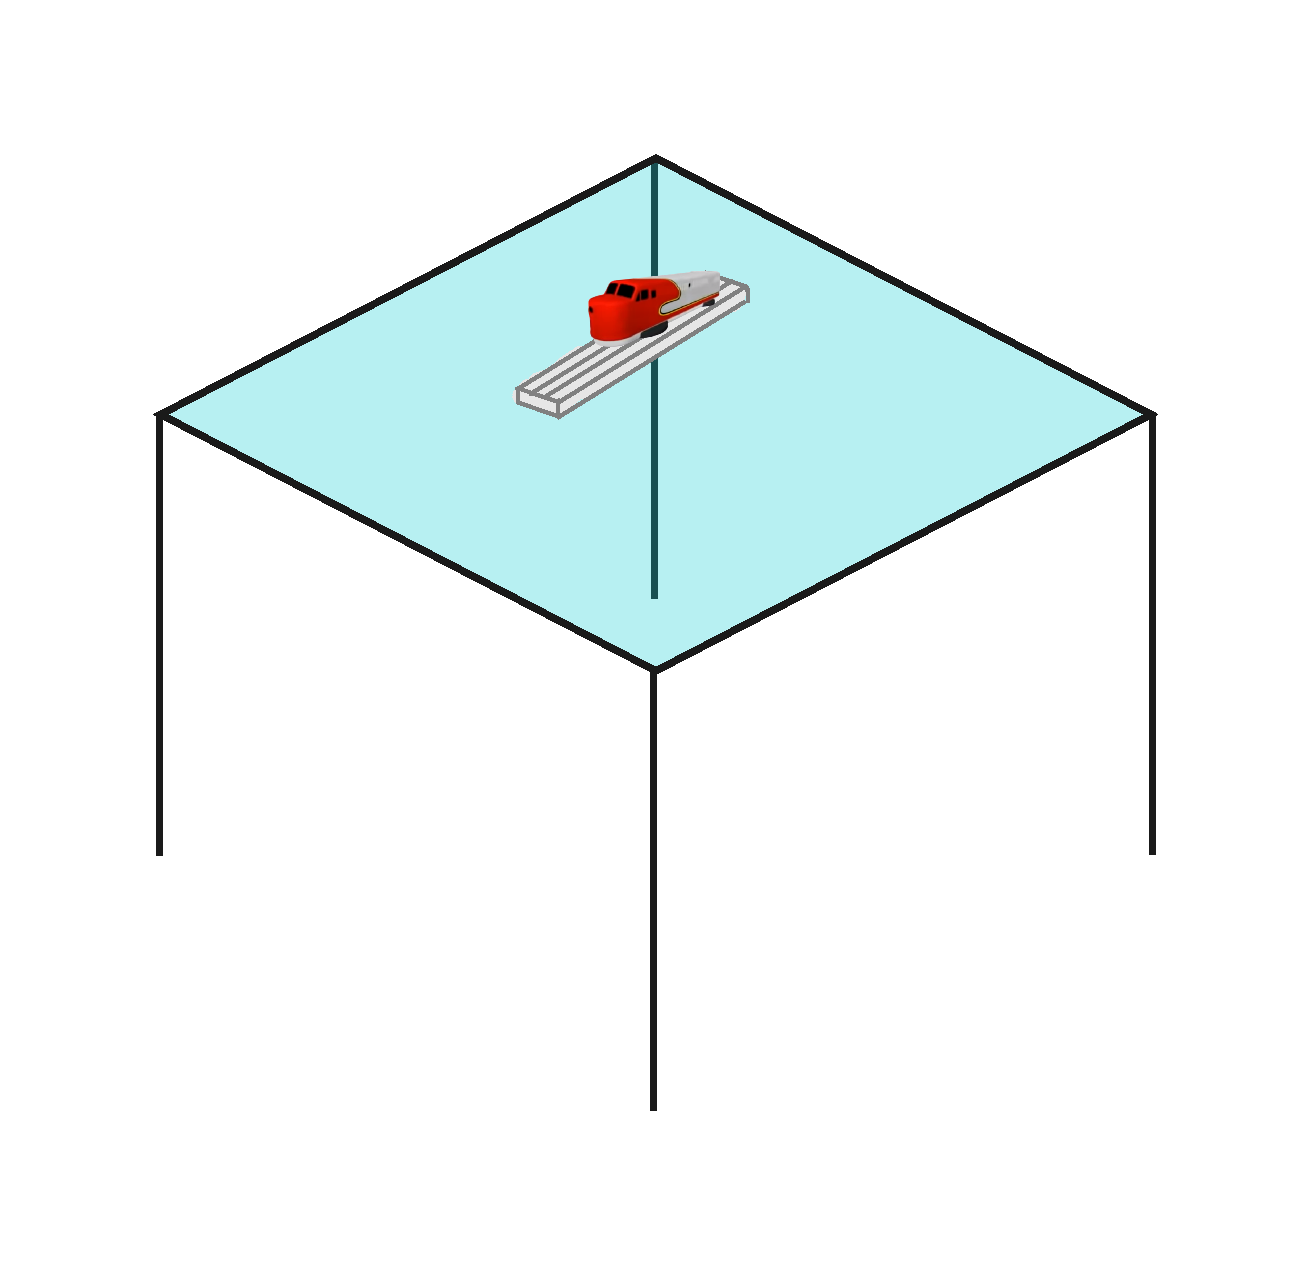
\includegraphics[scale=0.35]{table}
  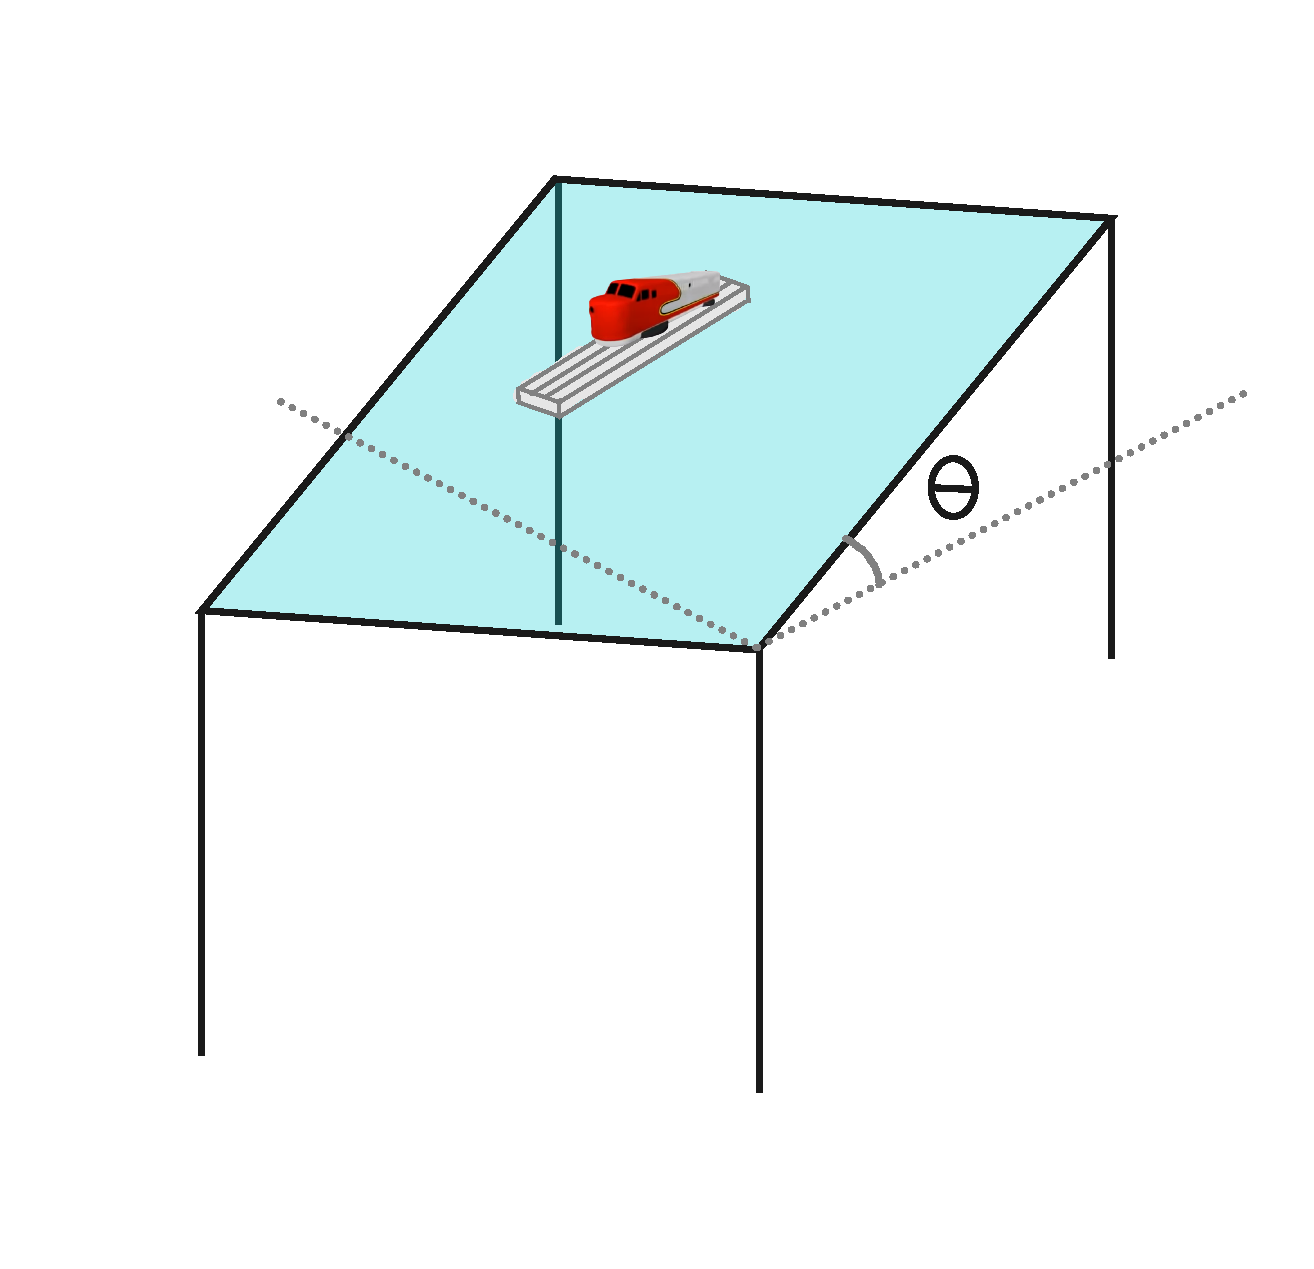
\includegraphics[scale=0.35]{tabletheta}
  \caption{Rotación de sistema de coordenadas}
  \label{fig:tabla}
\end{figure}




\begin{figure}
  \centering
  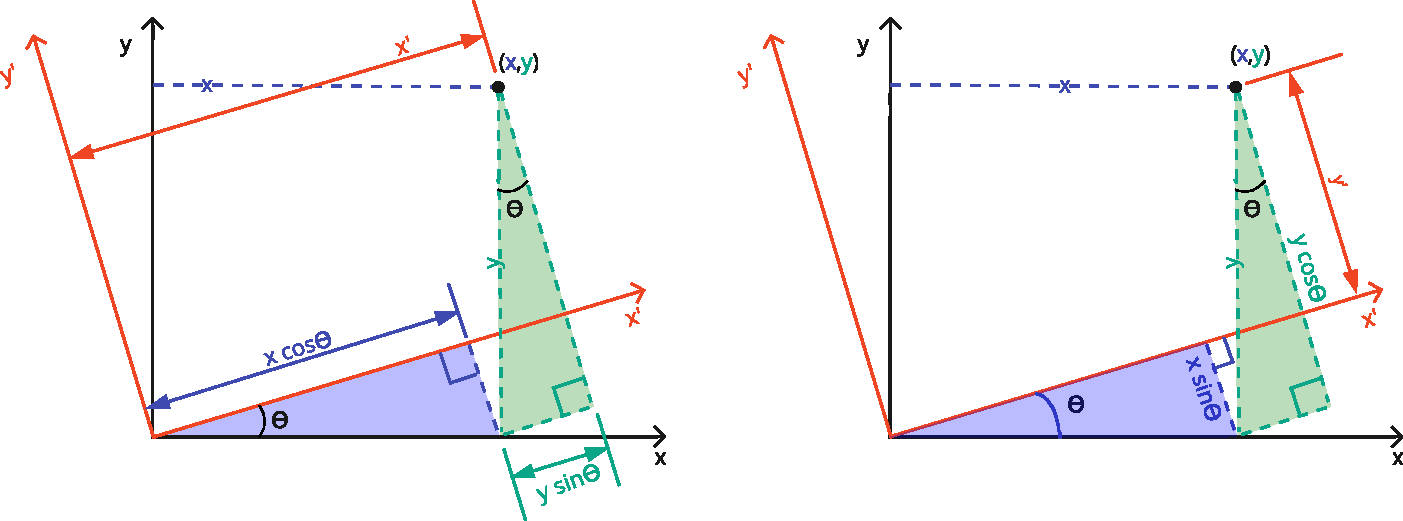
\includegraphics[scale=0.75]{so2}
  \caption{Rotación por ángulo $\theta$}
  \label{fig:so2}
\end{figure}



Considere un punto $(x,y)$ en sistema de referencia de dos dimensiones. Si cambiamos a un sistema de referencia rotado por un ángulo $\theta$, $(x',y')$, como se muestra en la figura~\ref{fig:so2}, podemos definir los dos triángulos rectángulos que se muestran en la figura y a partir de ellos obtener la transformación de los sistemas de referencia debido a la rotación
\begin{align}
  x'=&x\cos\theta+y\sin\theta \nonumber\\
  y'=&y\cos\theta-x\sin\theta\,.
\end{align}

% --- Inicio del código para insertar ---

% Para las ecuaciones matemáticas
\begin{align*}
    \boldsymbol{r} &= (x, y) \\
    \boldsymbol{r}' &= (x', y') \\[1em] % Añade un poco de espacio vertical
    r^2 = \boldsymbol{r} \cdot \boldsymbol{r} &= x^2 + y^2 \\
  {r'}^2 =  \boldsymbol{r}' \cdot \boldsymbol{r}' &= x'^2 + y'^2 = x^2 + y^2 = \boldsymbol{r} \cdot \boldsymbol{r}
\end{align*}

La demostración del último paso se hace a continuación.

% --- Inicio del código para insertar ---

\section*{Demostración de la Invariancia del Producto Escalar bajo Rotación}

El objetivo es demostrar que el módulo al cuadrado de un vector es el mismo después de una rotación de coordenadas. Es decir, probaremos que:
\[
\boldsymbol{r}' \cdot \boldsymbol{r}' = \boldsymbol{r} \cdot \boldsymbol{r} \quad \Leftrightarrow \quad x'^2 + y'^2 = x^2 + y^2
\]

\subsection*{Paso 1: Ecuaciones de Transformación por Rotación}
Las coordenadas $(x', y')$ en un sistema que ha sido rotado un ángulo $\theta$ en sentido antihorario se relacionan con las coordenadas originales $(x, y)$ mediante:
\begin{align*}
    x' &= x \cos\theta + y \sin\theta \\
    y' &= -x \sin\theta + y \cos\theta
\end{align*}

\subsection*{Paso 2: Sustitución y Expansión Algebraica}
Sustituimos estas transformaciones en la expresión para el módulo al cuadrado en el sistema rotado, $\boldsymbol{r}' \cdot \boldsymbol{r}' = x'^2 + y'^2$.

\begin{align*}
    x'^2 + y'^2 &= (x \cos\theta + y \sin\theta)^2 + (-x \sin\theta + y \cos\theta)^2 \\[1em]
    % Expandiendo los binomios al cuadrado
    &= (x^2 \cos^2\theta + 2xy \cos\theta \sin\theta + y^2 \sin^2\theta) \\
    &\quad + (x^2 \sin^2\theta - 2xy \sin\theta \cos\theta + y^2 \cos^2\theta) \\[1em]
    % Agrupando términos semejantes
    &= (x^2 \cos^2\theta + x^2 \sin^2\theta) + (y^2 \sin^2\theta + y^2 \cos^2\theta) \\
    &\quad + (2xy \cos\theta \sin\theta - 2xy \sin\theta \cos\theta) \\[1em]
    % Factorizando y cancelando
    &= x^2(\cos^2\theta + \sin^2\theta) + y^2(\sin^2\theta + \cos^2\theta) + \cancel{2xy \cos\theta \sin\theta} - \cancel{2xy \sin\theta \cos\theta} \\[1em]
    % Aplicando la identidad trigonométrica fundamental (sin^2 + cos^2 = 1)
    &= x^2(1) + y^2(1) \\[1em]
    % Resultado final
    &= x^2 + y^2
\end{align*}

\subsection*{Paso 3: Conclusión}
Hemos demostrado que $x'^2 + y'^2 = x^2 + y^2$. Por lo tanto, podemos concluir que el producto escalar es una cantidad invariante bajo rotaciones:
\begin{align}
\label{eq:so3}
    \boxed{
{r'}^2=\boldsymbol{r}' \cdot \boldsymbol{r}' = x'^2 + y'^2 = x^2 + y^2 = \boldsymbol{r} \cdot \boldsymbol{r} = r^2
}
\end{align}

% --- Fin del código para insertar ---

% Para el texto de conclusión
\vspace{1em} % Añade un poco más de espacio vertical
\noindent % Evita la sangría del párrafo
\textit{¡El producto escalar es invariante con respecto al sistema de coordenadas rotado!}

% --- Fin del código para insertar ---

Note que por consiguiente, la velocidad al cuadrado en la fórmula para la energía cinética (que se verá en detalle luego) es invariante bajo rotaciones del sistema de coordenadas
\begin{align*}
    E =\frac{1}{2}m v^2\,.
\end{align*}

En el Capítulo \ref{chap:relatividad} buscaremos qué cantidad permanece invariante bajo transformaciones entre observadores en movimiento, de forma análoga a como $r^2$ permaneció invariante aquí bajo rotación

\section{Ejercicios}

A continuación, se presentan veinte ejercicios propuestos para afianzar los conceptos fundamentales de unidades físicas, factores de conversión y análisis vectorial abordados en este capítulo. Recuerde prestar especial atención a las unidades en cada paso de sus cálculos.

\subsection*{Unidades Físicas y Factores de Conversión}

\begin{enumerate}
    \item \textbf{Conversión de Velocidad:} El límite de velocidad en muchas carreteras de Colombia es de $80 \text{ km/h}$. Utilizando factores de conversión, exprese esta velocidad en metros por segundo ($\text{m/s}$).
    
    \item \textbf{Conversión de Área y Volumen:} Un panel solar tiene un área de $2500 \text{ cm}^2$. Exprese esta área en metros cuadrados ($\text{m}^2$). Si una batería almacena un volumen de electrolito de $5 \text{ litros}$, ¿cuántos metros cúbicos ($\text{m}^3$) representa? (Recuerde que $1 \text{ L} = 1000 \text{ cm}^3$).
    
    \item \textbf{Análisis Dimensional:} La energía cinética se define algebraicamente como $K = \frac{1}{2}mv^2$, donde $m$ es la masa y $v$ es la magnitud de la velocidad. Demuestre, analizando las unidades, que esta expresión da como resultado unidades de Joules ($\text{J}$) en el Sistema Internacional.
    
    \item \textbf{Conversión a Electronvoltios:} En física nuclear, una partícula alfa es expulsada de un núcleo con una energía de $8.0 \times 10^{-13} \text{ J}$. Sabiendo que $1 \text{ eV} = 1.602 \times 10^{-19} \text{ J}$, exprese esta energía en mega-electronvoltios ($\text{MeV}$).
    
    \item \textbf{Unidades Naturales (Masa):} El Bosón de Higgs tiene una masa teórica de aproximadamente $125 \text{ GeV}/c^2$. Utilizando los factores de conversión del Sistema de Unidades Naturales dados en el texto, calcule la masa del Bosón de Higgs en kilogramos ($\text{kg}$).
    
    \item \textbf{Unidades Naturales (Distancia):} Si el radio de un átomo de hidrógeno es de aproximadamente $0.53 \times 10^{-10} \text{ m}$, utilice el factor de conversión $1 \text{ m} = 5.067 \times 10^6 \frac{\hbar c}{\text{eV}}$ para expresar este radio atómico en unidades de $\frac{\hbar c}{\text{eV}}$.
\end{enumerate}

\subsection*{Componentes, Magnitud y Dirección de Vectores}


\begin{enumerate}
    \setcounter{enumi}{6}
    \item \textbf{Magnitud y Dirección:} Una fuerza aplicada sobre un objeto está dada por el vector $\boldsymbol{F} = (6, -8) \text{ N}$. Calcule la magnitud de la fuerza $|\boldsymbol{F}|$ y el ángulo $\theta$ que forma con el eje $x$ positivo.
    
    \item \textbf{Descomposición Vectorial:} Un dron despega volando en línea recta a una rapidez de $15 \text{ m/s}$ con un ángulo de elevación de $60^\circ$ respecto a la horizontal. Encuentre las componentes rectangulares de su vector velocidad, $\boldsymbol{v} = (v_x, v_y)$.
    
    \item \textbf{Desplazamiento Resultante:} Un estudiante camina $4 \text{ km}$ hacia el Este (dirección $+x$) y luego $3 \text{ km}$ hacia el Norte (dirección $+y$). Escriba el vector de desplazamiento final $\boldsymbol{d}$ y calcule la distancia total en línea recta desde su punto de partida hasta su destino.
    
    \item \textbf{Vectores de Posición:} Un barco se encuentra en la coordenada $\boldsymbol{r}_A = (-5, 12) \text{ km}$ respecto al faro principal del puerto. ¿A qué distancia exacta ($|\boldsymbol{r}_A|$) se encuentra el barco del faro?
\end{enumerate}

\subsection*{Suma y Diferencia de Vectores}

\begin{enumerate}
    \setcounter{enumi}{10}
    \item \textbf{Suma de Fuerzas:} Sobre un objeto actúan dos fuerzas simultáneamente: $\boldsymbol{F}_1 = (12, 5) \text{ N}$ y $\boldsymbol{F}_2 = (-4, 3) \text{ N}$. Calcule el vector de la fuerza neta (resultante) $\boldsymbol{F}_{\text{neta}} = \boldsymbol{F}_1 + \boldsymbol{F}_2$ y encuentre su magnitud.
    
    \item \textbf{Posición Relativa:} El vehículo A se encuentra en la posición $\boldsymbol{r}_A = (10, 5) \text{ m}$ y el vehículo B se encuentra en $\boldsymbol{r}_B = (3, 29) \text{ m}$. Calcule el vector de desplazamiento relativo de A con respecto a B, es decir, $\Delta\boldsymbol{r}_{AB} = \boldsymbol{r}_A - \boldsymbol{r}_B$.
    
    \item \textbf{Equilibrio de Fuerzas:} Para que un puente se mantenga estático, la suma de todas las fuerzas que actúan sobre un nodo debe ser cero ($\boldsymbol{F}_{\text{neta}} = \boldsymbol{0}$). Si dos cables ejercen fuerzas $\boldsymbol{F}_1 = (500, 200) \text{ N}$ y $\boldsymbol{F}_2 = (-300, 150) \text{ N}$, ¿cuál debe ser el vector de fuerza $\boldsymbol{F}_3$ del pilar de soporte para que el sistema esté en equilibrio?
    
    \item \textbf{Propiedades Algebraicas:} Dados los vectores $\boldsymbol{u} = (2, -3)$ y $\boldsymbol{v} = (-1, 4)$, demuestre algebraicamente que la suma de vectores es conmutativa verificando que $\boldsymbol{u} + \boldsymbol{v} = \boldsymbol{v} + \boldsymbol{u}$.
\end{enumerate}

\subsection*{Producto Escalar y Trabajo}

\begin{enumerate}
    \setcounter{enumi}{14}
    \item \textbf{Producto Escalar Analítico:} Dados los vectores de fuerza $\boldsymbol{F} = (4, -2) \text{ N}$ y de desplazamiento $\Delta\boldsymbol{r} = (3, 5) \text{ m}$, calcule el trabajo mecánico realizado utilizando la definición algebraica del producto escalar: $W = \boldsymbol{F} \cdot \Delta\boldsymbol{r}$.
    
    \item \textbf{Producto Escalar Geométrico:} Una persona arrastra una caja aplicando una fuerza de magnitud $|\boldsymbol{F}| = 150 \text{ N}$ mediante una cuerda que forma un ángulo de $30^\circ$ con el suelo horizontal. Si la caja se desplaza una distancia de $|\Delta\boldsymbol{r}| = 10 \text{ m}$, calcule el trabajo realizado usando la definición geométrica $W = |\boldsymbol{F}| |\Delta\boldsymbol{r}| \cos\theta$.
    
    \item \textbf{Ángulo entre Vectores:} Utilizando la relación geométrica del producto escalar ($\boldsymbol{u} \cdot \boldsymbol{v} = |\boldsymbol{u}| |\boldsymbol{v}| \cos\theta$), encuentre el ángulo $\theta$ formado entre los vectores $\boldsymbol{u} = (3, 0)$ y $\boldsymbol{v} = (3, 3)$.
\end{enumerate}

\subsection*{Producto Vectorial y Torque}

\begin{enumerate}
    \setcounter{enumi}{17}
    \item \textbf{Magnitud del Torque:} Un mecánico intenta aflojar una tuerca muy apretada utilizando una llave inglesa de longitud $|\boldsymbol{r}| = 0.40 \text{ m}$. Si aplica una fuerza máxima de $|\boldsymbol{F}| = 200 \text{ N}$ en el extremo de la llave con un ángulo de $60^\circ$ respecto al mango, calcule la magnitud del torque generado ($|\boldsymbol{\tau}| = |\boldsymbol{r}| |\boldsymbol{F}| \sin\theta$).
    
    \item \textbf{Regla de la Mano Derecha:} Una partícula cargada positivamente se mueve a lo largo del eje $+x$ (hacia la derecha) con una velocidad $\boldsymbol{v}$. Entra en una región donde existe un campo magnético $\boldsymbol{B}$ que apunta directamente a lo largo del eje $+y$ (hacia arriba). Sabiendo que la fuerza magnética viene dada por $\boldsymbol{F} = q(\boldsymbol{v} \times \boldsymbol{B})$, utilice la regla de la mano derecha para determinar en qué dirección apuntará el vector de fuerza $\boldsymbol{F}$ en el espacio 3D. (NOTA: no necesitas entender el electromagnetismo, solo aplicar la regla geométrica)
    
    \item \textbf{Maximización del Producto Vectorial:} Si la magnitud del producto cruz es $|\boldsymbol{u} \times \boldsymbol{v}| = |\boldsymbol{u}| |\boldsymbol{v}| \sin\theta$, responda conceptualmente: 
    \begin{enumerate}
        \item ¿Qué ángulo $\theta$ entre $0^\circ$ y $180^\circ$ maximiza el resultado del producto vectorial?
        \item ¿Qué condición geométrica debe cumplirse entre $\boldsymbol{u}$ y $\boldsymbol{v}$ para que su producto vectorial sea exactamente cero?
    \end{enumerate}

\end{enumerate}


\chapter{Relatividad especial}
\label{chap:relatividad}

\section{Introducción}
Las transformaciones de Lorentz son la piedra angular de la teoría de la Relatividad Especial de Einstein. Relacionan las coordenadas de espacio y tiempo de un evento según lo medido por dos observadores en diferentes sistemas de referencia inerciales. Reemplazan a las antiguas transformaciones de Galileo, que son inconsistentes con la constancia observada de la velocidad de la luz.

La derivación se basa en dos postulados fundamentales de la Relatividad Especial:
\begin{enumerate}
    \item \textbf{El Principio de Relatividad:} Las leyes de la física son las mismas en todos los sistemas de referencia inerciales.
    \item \textbf{La Constancia de la Velocidad de la Luz:} La velocidad de la luz en el vacío, denotada por $c$, es la misma para todos los observadores inerciales, independientemente del movimiento de la fuente de luz o del observador.
\end{enumerate}

El segundo principio puede ser cambiado simplemente por la suposición de que el espacio y el tiempo deben ser homogéneos e isotrópicos, ver \url{https://arxiv.org/pdf/gr-qc/0107091}

La motivación de la relatividad especial surge de la necesidad de usar el primer postulado para la interacción electromagnética. Aunque dicho postulado es evidente en sistemas mecánicos, no es claro para la interacción electromagnética. De hecho, una partícula cargada en reposo sólo tiene asociado un campo eléctrico, mientras que una partícula moviéndose a velocidad constante relativa al observador en reposo, genera una corriente eléctrica que a su vez induce un campo magnético. Además, el campo eléctrico se deforma (las regiones de campo constante pasan de ser esféricas a elipsoidales). Como en última instancia los objetos de medida están hechos de partículas cargadas dentro de los átomos que la componen, es de esperarse que sean afectadas por el movimiento aunque éste sea a velocidad constante.


\section{Transformaciones de Lorentz}

Consideremos dos sistemas de referencia inerciales, $S$ y $S'$.
\begin{itemize}
    \item El sistema $S$ tiene coordenadas $(x, y, z, t)$.
    \item El sistema $S'$ tiene coordenadas $(x', y', z', t')$.
\end{itemize}
Configuramos los sistemas de tal manera que $S'$ se mueve con una velocidad constante $\boldsymbol{v}$ relativa a $S$ a lo largo del eje x positivo. En el tiempo $t=t'=0$, los orígenes de los dos sistemas coinciden.
\[
\text{Sistema S} \quad \xrightarrow{v} \quad \text{Sistema S'}
\]
Dado que el movimiento relativo es solo a lo largo del eje x, las coordenadas perpendiculares al movimiento no se ven afectadas:
\[ y' = y, \quad z' = z \]

\begin{figure}
% --- Inicio del código TikZ para insertar ---
%\begin{center}
\centering
\begin{tikzpicture}[
    scale=1.2,          % Escala general de la figura
    font=\Large,        % Tamaño de la fuente para las etiquetas
    axis/.style={->, thick}, % Estilo para los ejes (flecha, grueso)
]

% --- Sistema de referencia S (estacionario, en gris) ---
% Eje horizontal x
\draw[axis, black] (0,0) -- (3,0) node[below, black, pos=0.8] {$x$};
% Eje vertical t
\draw[axis, black] (0,0) -- (0,3) node[left] {$t$};
% Etiqueta del sistema
\node[black, anchor=south east] at (0,3.1) {$S$};

% --- Sistema de referencia S' (en movimiento, en rojo) ---
% Usamos un 'scope' con 'xshift' para mover todo el sistema S'
\begin{scope}[xshift=1.5cm,yshift=0.1cm]
    % Eje horizontal x'
    \draw[axis, red] (0,0) -- (3,0) node[below, black, pos=0.8] {$x'$};
    % Eje vertical t'
    \draw[axis, red] (0,0) -- (0,3) node[left] {$t'$};
    % Etiqueta del sistema
    \node[red, anchor=south west] at (0,3.1) {$S'$};
\end{scope}

% --- Flecha de velocidad v ---
\draw[axis, black] (1.7, 1.5) -- (2.7, 1.5) node[midway, above] {$v$};

% --- Punto del evento ---
\fill[black] (4.5, 2.2) circle (3.5pt);

% --- distancia entre sistemas ---
\draw[axis, gray] (0.5, 0.5) -- (0.0, 0.5) node[midway, ,gray,pos=-0.5] {$vt$};
\draw[axis, gray] (1.0, 0.5) -- (1.5, 0.5);



\end{tikzpicture}
%\end{center}
% --- Fin del código TikZ ---
    \caption{Sistema de referencia inercial $\color{red}S'$, a velocidad constante en $x$, $v$, con respecto al sistema en reposo $S$. A un tiempo $t$ el origin de $\color{red}S'$ se encuentra a una distancia $x = vt$ del origen de $S$. }
    \label{fig:placeholder}
\end{figure}


Ahora nos enfocamos en derivar las transformaciones para $x'$ y $t'$.

\section{Pasos de la Derivación}

\subsection{Paso 1: La Suposición de Linealidad}

Las transformaciones deben ser lineales para preservar el principio de inercia. Un movimiento uniforme en un sistema debe aparecer como un movimiento uniforme en el otro. Por lo tanto, las transformaciones tienen la forma:
\begin{align}
\label{eq:tl1}
 x' = Ax + Bt\,.   
\end{align}
 
\subsection{Paso 2: Usando el Movimiento del Origen}

El origen de $S'$ ($x'=0$) se mueve con velocidad $v$ en el sistema $S$, por lo que su posición es $x=vt$. Sustituyendo esto en la ecuación~\eqref{eq:tl1}:
\[ 0 = A(vt) + Bt \implies B = -Av \]
Esto da $x' = A(x-vt)$. Renombramos la constante $A$ con el símbolo más convencional $\gamma$.
\begin{align}
\label{eq:xplt}
x' = \gamma (x - vt).    
\end{align}

\subsection{Paso 3: Aplicando el Principio de Relatividad}

La transformación inversa (de $S'$ a $S$) debe tener la misma forma, con la velocidad invertida ($v \to -v$):
\begin{align}
\label{eq:invxplt}
    x = \gamma (x' + vt').
\end{align}

\subsection{Paso 4: Aplicando el Segundo Postulado}
Imaginemos un pulso de luz emitido desde el origen en $t=t'=0$. Un observador en $S$ ve su frente de onda en $x=ct$, mientras que un observador en $S'$ lo ve en $x'=ct'$. Sustituyendo esto en nuestras ecuaciones de transformación:

\newcounter{paso}

\noindent
%\renewcommand{\phantom}[1]{#1}
%\renewcommand{\arraystretch}{1.5}
\begin{tabular}{l|p{0.35\textwidth}|p{0.6\textwidth}}
\textbf{Paso}&\textbf{Encontrar} $\gamma$& \textbf{Paso algebraico} \\\hline
\stepcounter{paso}\thepaso)&$\begin{aligned}
    x' =& \gamma (x - vt),\\
    x = &\gamma (x' + vt').
\end{aligned}$& Ecuaciones \eqref{eq:xplt} y \eqref{eq:invxplt}\\\hline
\stepcounter{paso}\thepaso)&$\begin{aligned}[t]
ct' &= \gamma(ct - vt) = \gamma t (c-v)  \\
ct &= \gamma(ct' + vt') = \gamma t' (c+v)  
\end{aligned}$  &  Reemplazando $x=ct$ y $x'=ct'$ en  
las ecuaciones anteriores\\\hline
\stepcounter{paso}\thepaso)&$(ct')(ct) = [\gamma t (c-v)][\gamma t' (c+v)]$& Multiplicando las dos ecuaciones\\\hline
\stepcounter{paso}\thepaso)&$c^2 t' t = \gamma^2 t t' (c-v)(c+v)$& 
Realizando las operaciones indicadas\\\hline
\stepcounter{paso}\thepaso)&$c^2= \gamma^2 (c^2-v^2)$& Dividiendo por $tt'$ a ambos lados de la igualdad y expandiendo la diferencia de cuadrados \\\hline
\stepcounter{paso}\thepaso)&$1=\gamma^2(1-v^2/c^2)$&Dividiendo por $c^2$ a ambos lados de la igualdad.\\\hline
\stepcounter{paso}\thepaso)&$\gamma^2 = \dfrac{1}{1-v^2/c^2}$&
Dividiendo por $1-v^2/c^2$ a ambos lados de la igualdad.
\\[8pt]\hline
\stepcounter{paso}\thepaso)&$\gamma = \dfrac{1}{\sqrt{1-v^2/c^2}}$&
Sacando raíz cuadrada a ambos lados iguales\\[8pt]\hline
\end{tabular}

De ésta forma obtenemos el \emph{factor de Lorentz}
\begin{align}
\label{eq:gamma}
    \boxed{\gamma = \frac{1}{\sqrt{1 - \beta^2}}} \,,
\end{align}
donde
\begin{align}
    \label{eq:beta}
    \beta =\frac{v}{c}\,,
\end{align}
y 
\begin{align}
\label{eq:gammasquare}
    \gamma^2 =&\frac{1}{1-\dfrac{v^2}{c^2}} =  
    \frac{\dfrac{1}{1}}{\dfrac{c^2-v^2}{c^2}}=
    \frac{c^2}{c^2-v^2}\,.
\end{align}

Podemos ver que el factor de Lorentz, $\gamma$, varía desde el valor $1$ cuando $v\ll c$, o $c\to \infty$, hasta $\infty$ cuando $v\to c$, como se ilustra en la figura~\ref{fig:gammafactor}. La función $\gamma$ no tiene valores reales para $v>c$. Por consiguiente, $v=c$ se considera la velocidad límite para un sistema de referencia inercial, una velocidad que no se puede superar por ningún objeto material.

\begin{figure}
    \centering
\begin{tikzpicture}
    \begin{axis}[
        width=7cm,
        height=7cm,
        % Etiquetas de los ejes
        xlabel={Velocidad del sistema inercial ($v$)},
        ylabel={Factor de Lorentz ($\gamma$)},
        % Rango de los ejes (usamos x = v/c, de 0 a 1)
        xmin=0, xmax=1.05,
        ymin=0, ymax=10,
        % Ticks (marcas) personalizados para el eje x en términos de c
        xtick={0, 0.2, 0.4, 0.6, 0.8, 1.0},
        xticklabels={0, $0.2c$, $0.4c$, $0.6c$, $0.8c$, $c$},
        % Ticks para el eje y
        ytick={1, 2, 4, 6, 8, 10},
        % Estilo de los ejes y cuadrícula
        axis lines=left,
        grid=both,
        grid style={dashed, gray!50},
        % Posición de la leyenda
        legend pos=north west,
        % Cantidad de puntos para suavizar la curva (crítico cerca de c)
        samples=200
    ]
    
    % Graficamos la función Gamma. 
    % El dominio va hasta 0.995 para evitar la división por cero en x=1
    \addplot[
        domain=0:0.9949, 
        color=blue, 
        thick
    ]
    {1 / sqrt(1 - x^2)};
    \addlegendentry{$\gamma = \frac{1}{\sqrt{1 - v^2/c^2}}$}

    % Dibujamos la asíntota vertical en v = c (x = 1)
    \draw[dashed, red, thick] (axis cs:1, 0) -- (axis cs:1, 10);
    
    % Añadimos un texto para la asíntota
    \node[red, anchor=south east, rotate=90] at (axis cs:0.97, 2) {Asíntota $v=c$};

    % Marcamos el punto de reposo (v=0, gamma=1)
    \addplot[mark=*, color=blue] coordinates {(0,1)};
    \node[anchor=south west] at (axis cs:0, 1) {$\gamma(0)=1$};

    \end{axis}
\end{tikzpicture}
 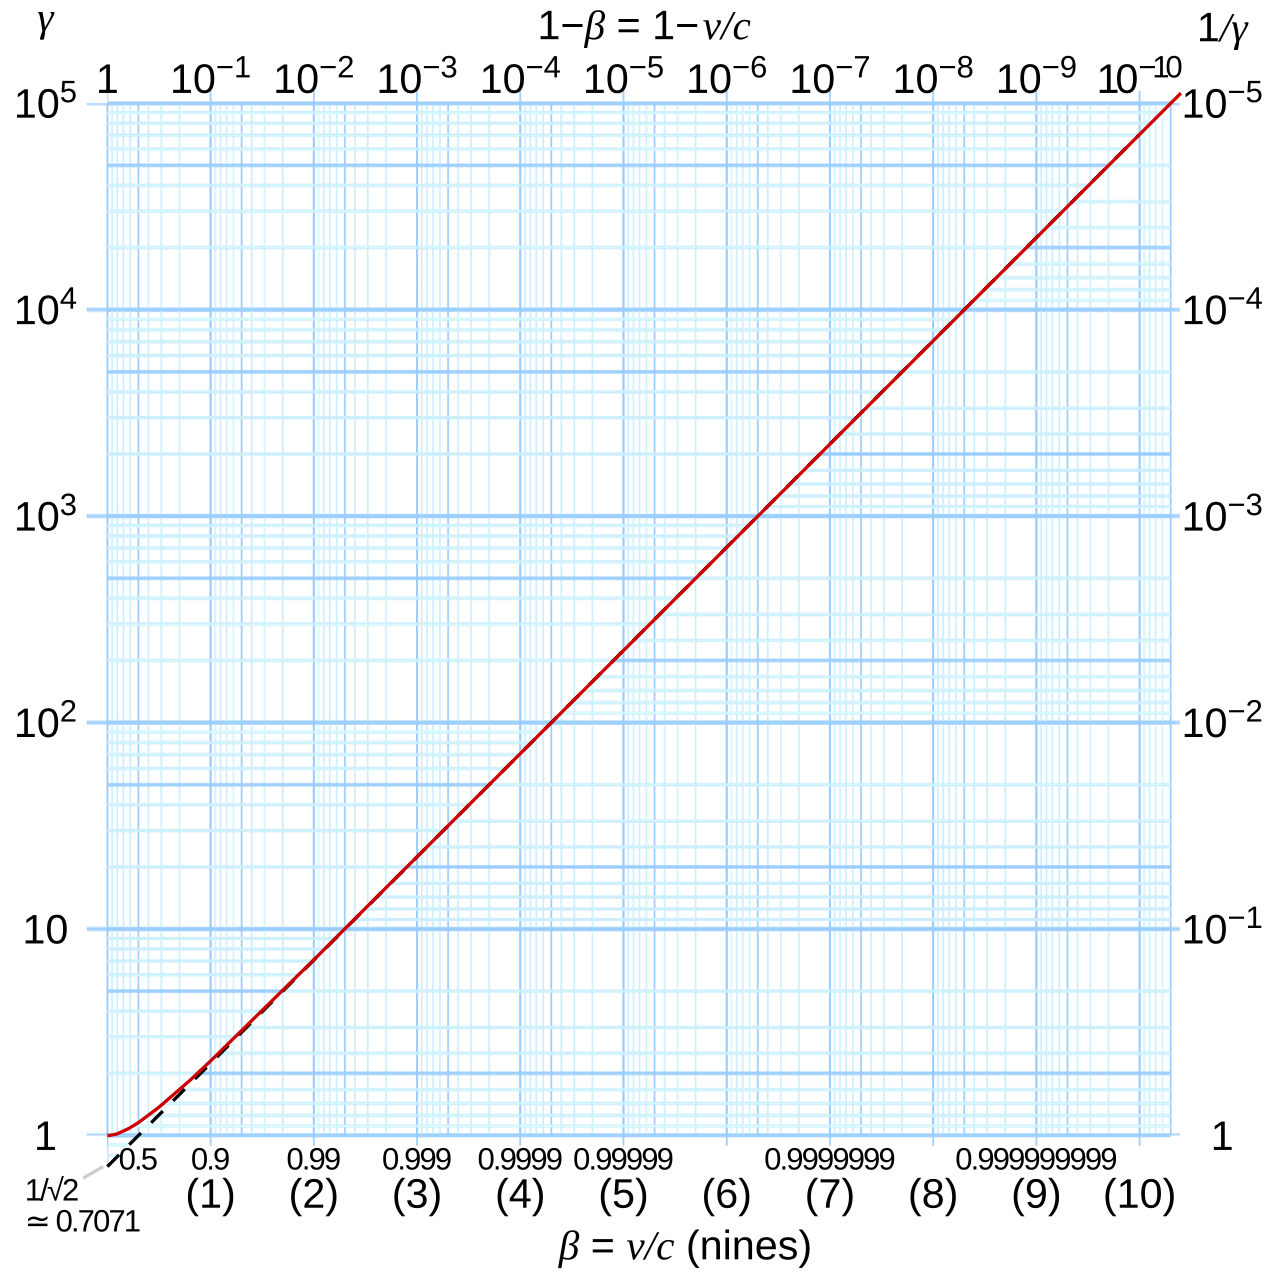
\includegraphics[scale=0.16]{Lorentz_factor_log_log}
    \caption{Factor de Lorentz. Versión log-log de Wikipedia}
    \label{fig:gammafactor}
\end{figure}

\subsection{Paso 6: Derivando la Transformación del Tiempo}
Dado que ya tenemos la expresión completa para $x'$, en las ecuaciones \eqref{eq:xplt} y \eqref{eq:invxplt}, podemos
despejar $t'$

\subsubsection*{Ejercicio}
Complete los pasos que faltan en la derivación en la siguiente tabla

%\renewcommand{\phantom}[1]{#1}
\noindent
\setcounter{paso}{0}
\begin{tabular}{l|p{0.35\textwidth}|p{0.6\textwidth}}
\textbf{paso} &\textbf{Despejar} $t'$& \textbf{Paso algebraico} \\\hline
\stepcounter{paso}\thepaso) & $\begin{aligned}
    x' =& \gamma (x - vt),\\
    x = &\gamma (x' + vt').
\end{aligned}$& Ecuaciones \eqref{eq:xplt} y \eqref{eq:invxplt}\\\hline
\stepcounter{paso}\thepaso) & \phantom{ $x=\gamma[\gamma(x-vt) +v t']$}&Sustituyendo $x'=\gamma(x-vt)$ en $x = \gamma(x' + vt')$\\\hline
\stepcounter{paso}\thepaso) & $x=\gamma^2x-\gamma^2 vt +\gamma v t'$  & Distribuyendo $\gamma$ el lado derecho\\\hline
\stepcounter{paso}\thepaso) & \phantom{$\gamma v t' = x-\gamma^2x +\gamma^2 v t$} & Sumando $-\gamma^2x +\gamma^2 v t$ a ambos lados de la igualdad. \\\hline
\stepcounter{paso}\thepaso) & $\gamma v t' = x(1-\gamma^2) +\gamma^2 v t$  & Factorizando $x$.\\\hline
\stepcounter{paso}\thepaso) & \phantom{$\gamma v t' = x\left(1-\dfrac{c^2}{c^2-v^2}\right) +\gamma^2 v t$} & Reemplazando $\gamma^2=\dfrac{c^2}{c^2-v^2}$ en el término en $x$ \\\hline
\stepcounter{paso}\thepaso) & $\gamma v t' = x\left(\dfrac{\cancel{c^2}-v^2-\cancel{c^2}}{c^2-v^2}\right) +\gamma^2 v t$. & Sumando las fracciones y cancelando $c^2$ en el numerador\\\hline
\stepcounter{paso}\thepaso) & \phantom{$\gamma v t' =\gamma^2 v t- xv^2\left[\dfrac{c^2}{c^2(c^2-v^2)}\right]$} & Multiplicando y dividiendo por $c^2$ en el término que multiplica a $x$ \\[5pt]\hline
\stepcounter{paso}\thepaso) & ${\gamma}{v}  t' =\gamma^{{2}}{v}  t- \gamma^{{2}} \dfrac{v^2 x}{c^2}$  &
Recuperando $\gamma^2$ a partir de $\dfrac{c^2}{c^2-v^2}$ \\\hline
\stepcounter{paso}\thepaso) & \phantom{$t' = \gamma t-\dfrac{vx}{c^2}$} & Dividiendo a  a ambos lados de la igualdad por $\gamma v$ \\[5pt]\hline
\stepcounter{paso}\thepaso) & $t' = \gamma\left(t-\dfrac{vx}{c^2}\right)$&Factorizando $\gamma$\\[5pt]\hline
\end{tabular}

De modo que
\[ \boxed{t' = \gamma \left( t - \frac{vx}{c^2} \right)} \]

\section{Resumen de las Transformaciones de Lorentz}
Las transformaciones de Lorentz completas son:
\[
\boxed{
\begin{aligned}
t' &= \gamma \left( t - \frac{vx}{c^2} \right) \\
x' &= \gamma (x - vt) \\
y' &= y \\
z' &= z
\end{aligned}
}
\]

\subsection{Las Transformaciones Inversas}
Las transformaciones de $S'$ a $S$ se encuentran intercambiando las coordenadas y haciendo $v \to -v$:
\[
\boxed{
\begin{aligned}
t &= \gamma \left( t' + \frac{vx'}{c^2} \right) \\
x &= \gamma (x' + vt') \\
y &= y' \\
z &= z'
\end{aligned}
}
\]

\subsection{Transformaciones de Galileo}
Se obtienen cuando no hay una velocidad límite, y por lo tanto $c\to \infty$
\begin{align*}
t' &= \lim_{c\to\infty}\left[\gamma \left( t - \frac{vx}{c^2} \right)\right] 
    = t\\
x' &= \lim_{c\to\infty}\left[\gamma (x - vt)\right]  = x - vt \\
y' &= y \\
z' &= z
\end{align*}

Mientras que para factor de Lorentz $\gamma$, o el factor de contracción relativista $1/\gamma$, 
\begin{align}
    \lim_{c\to\infty}\ \gamma = 1\,. 
\end{align}

Esto quiere decir que las las distancia y tiempos no están afectados por las transformaciones de Galileo.

\subsection{Existencia de una velocidad límite en el Universo}

Toda la evidencia experimental, desde el electromagnetismo hasta la desintegración de partículas, confirma que vivimos en un universo donde hay una velocidad límite. Llamamos a esta velocidad universal $c$, y la identificamos con la velocidad de la luz en el vacío. La constancia de la velocidad de la luz no es una suposición separada, sino una consecuencia directa de la estructura del espacio-tiempo mismo, como se demuestra en el Apendice~\ref{sec:tl}.




\section{Derivación de la Dilatación del Tiempo a partir de las Transformaciones de Lorentz}

En las aplicaciones prácticas, donde se estudia el movimiento de un cuerpo a velocidad constante, es conveniente asumir que el sistema inercial se mueve con la misma velocidad del cuerpo bajo estudio, como se ilustra en la figura~\ref{fig:movv}.

\begin{figure}
% --- Inicio del código TikZ para insertar ---
%\begin{center}
\centering
\begin{tikzpicture}[
    scale=1.2,          % Escala general de la figura
    font=\Large,        % Tamaño de la fuente para las etiquetas
    axis/.style={->, thick}, % Estilo para los ejes (flecha, grueso)
]

% --- Sistema de referencia S (estacionario, en gris) ---
% Eje horizontal x
\draw[axis, black] (0,0) -- (3,0) node[below, black, pos=0.8] {$x$};
% Eje vertical t
\draw[axis, black] (0,0) -- (0,3) node[left] {$t$};
% Etiqueta del sistema
\node[black, anchor=south east] at (0,3.1) {$S$};

% --- Sistema de referencia S' (en movimiento, en rojo) ---
% Usamos un 'scope' con 'xshift' para mover todo el sistema S'
\begin{scope}[xshift=1.5cm,yshift=0.1cm]
    % Eje horizontal x'
    \draw[axis, red] (0,0) -- (3.5,0) node[below, black, pos=0.8] {$x'$};
    % Eje vertical t'
    \draw[axis, red] (0,0) -- (0,3) node[left] {$t'$};
    % Etiqueta del sistema
    \node[red, anchor=south west] at (0,3.1) {$S'$};
\end{scope}

% --- Flecha de velocidad v ---
\draw[axis, black] (1.7, 1.5) -- (2.7, 1.5) node[midway, above] {$v$};

% --- Punto del evento ---
\fill[black] (1.7, 1.5) circle (3.5pt);

\node[inner sep=0pt] (russell) at (3.5,2)
    {
\includegraphics[scale=0.03]{clock}};

\draw[dotted] (3.5, 0.1) -- (3.5,2);

\node[black] (russell) at (3.5,-0.15) {$x'_c$};

\draw[axis, black] (3.7, 2) -- (4.7, 2) node[midway, above] {$v$};


\end{tikzpicture}
%\end{center}
% --- Fin del código TikZ ---
    \caption{Sistema de referencia inercial $\color{red}S'$, moviendos con velocidad constante en $x$, $v$, con el objeto bajo estudio }
    \label{fig:movv}
\end{figure}


La dilatación del tiempo es una consecuencia directa y famosa de las transformaciones de Lorentz. Describe el fenómeno en el que un reloj que está en movimiento relativo a un observador se mide por ese observador como si estuviera marcando el tiempo más lentamente que un reloj que está en reposo relativo a él.

Para derivar esto, estableceremos un experimento mental simple y aplicaremos la transformación de Lorentz para el tiempo.

\subsection{La Configuración Física (Experimento Mental)}

\begin{enumerate}
    \item \textbf{Dos Sistemas:} Tenemos dos sistemas inerciales, $S$ y $S'$. Como antes, el sistema $S$ es el sistema ``estacionario'' (por ejemplo, un observador en el suelo), y el sistema $S'$ se mueve con una velocidad constante $v$ a lo largo del eje x relativo a $S$.

    \item \textbf{Un Reloj en el Sistema en Movimiento:} Imaginemos que hay un reloj en reposo en el sistema en movimiento, $S'$. Dado que el reloj no se mueve \textit{dentro de su propio sistema}, su posición es un valor constante, que llamaremos $x'_c$.

    \item \textbf{Dos Eventos:} Consideraremos dos eventos, que son dos ``tictacs'' consecutivos de este reloj.
    \begin{itemize}
        \item \textbf{Evento 1:} El reloj hace tictac por primera vez. Desde la perspectiva de un observador en el sistema $S'$, este evento ocurre en las coordenadas $(t'_1, x'_c)$.
        \item \textbf{Evento 2:} El reloj hace tictac por segunda vez. En el sistema $S'$, este evento ocurre en las coordenadas $(t'_2, x'_c)$.
    \end{itemize}
\end{enumerate}

\subsection{Definiendo el Tiempo Propio}

El intervalo de tiempo entre dos eventos que ocurren en la \textbf{misma ubicación espacial} en un sistema dado se llama \textbf{intervalo de tiempo propio}, denotado por $\Delta t_0$. Por lo tanto, el tiempo propio es el tiempo que transcurre para un observador que viaja junto con el objeto en movimiento.

En nuestra configuración, los dos tictacs del reloj ocurren en la misma ubicación ($x'_c$) en el sistema $S'$. Por lo tanto, el intervalo de tiempo medido por un observador en el sistema en movimiento $S'$ es el tiempo propio:
\[ \Delta t_0 = t'_2 - t'_1 \]
Nuestro objetivo es encontrar el intervalo de tiempo entre estos mismos dos eventos según lo medido por el observador en el sistema estacionario $S$. Llamemos a este intervalo $\Delta t$.
\[ \Delta t = t_2 - t_1 \]

\subsection{Aplicando las Transformaciones de Lorentz}

Necesitamos relacionar las coordenadas de tiempo en $S$ con las coordenadas en $S'$. La transformación de Lorentz inversa para el tiempo es la opción más conveniente aquí, ya que expresa el tiempo del sistema estacionario ($t$) en términos de las coordenadas del sistema en movimiento ($t', x'$).
\[ t = \gamma \left( t' + \frac{vx'}{c^2} \right) \]
Ahora, aplicamos esta transformación a nuestros dos eventos:
\begin{enumerate}
    \item El tiempo del Evento 1 medido en el sistema $S$ es $t_1$:
    \[ t_1 = \gamma \left( t'_1 + \frac{vx'_c}{c^2} \right) \]
    \item El tiempo del Evento 2 medido en el sistema $S$ es $t_2$:
    \[ t_2 = \gamma \left( t'_2 + \frac{vx'_c}{c^2} \right) \]
\end{enumerate}

\subsection{La Derivación}

El intervalo de tiempo $\Delta t$ medido por el observador en el sistema $S$ es la diferencia entre $t_2$ y $t_1$.
\begin{align*}
\Delta t &= t_2 - t_1 \\
&= \left[ \gamma \left( t'_2 + \frac{vx'_c}{c^2} \right) \right] - \left[ \gamma \left( t'_1 + \frac{vx'_c}{c^2} \right) \right] \\
&= \gamma \left( t'_2 + \frac{vx'_c}{c^2} - t'_1 - \frac{vx'_c}{c^2} \right) \\
&= \gamma (t'_2 - t'_1)
\end{align*}
El término que involucra la posición $x'_c$ se cancela precisamente porque el reloj estaba en reposo en el sistema $S'$. Ahora sustituimos la definición de tiempo propio, $\Delta t_0 = t'_2 - t'_1$:
\[ \Delta t = \gamma \Delta t_0 \]

\subsection{Resultado e Interpretación}

La fórmula final para la dilatación del tiempo se obtiene sustituyendo la expresión para $\gamma$:
\[ \boxed{ \Delta t = \frac{\Delta t_0}{\sqrt{1 - v^2/c^2}} } \]
Interpretemos este importante resultado:
\begin{itemize}
    \item El factor de Lorentz $\gamma = \frac{1}{\sqrt{1 - v^2/c^2}}$ es siempre mayor o igual a 1, ya que la velocidad $v$ debe ser menor que $c$.
    \item Esto significa que $\Delta t \ge \Delta t_0$.
    \item El intervalo de tiempo ($\Delta t$) medido por el observador en el sistema ``estacionario'' $S$ es \textit{más largo} que el intervalo de tiempo propio ($\Delta t_0$) medido en el sistema de reposo del reloj.
\end{itemize}
Un intervalo de tiempo más largo entre tictacs significa que se observa que el reloj funciona más lentamente. Por lo tanto, el observador en $S$ concluye que el reloj en movimiento funciona lentamente en comparación con su propio reloj idéntico. Este fenómeno es la \textbf{dilatación del tiempo}.


\section{Derivación de la Contracción de la Longitud a partir de las Transformaciones de Lorentz}

\begin{figure}
% --- Inicio del código TikZ para insertar ---
%\begin{center}
\centering
\begin{tikzpicture}[
    scale=1.2,          % Escala general de la figura
    font=\Large,        % Tamaño de la fuente para las etiquetas
    axis/.style={->, thick}, % Estilo para los ejes (flecha, grueso)
]

% --- Sistema de referencia S (estacionario, en gris) ---
% Eje horizontal x
\draw[axis, black] (0,0) -- (4,0) node[below, black, pos=0.5] {$x$};
% Eje vertical t
\draw[axis, black] (0,0) -- (0,3) node[left] {$t$};
% Etiqueta del sistema
\node[black, anchor=south east] at (0,3.1) {$S$};

% --- Sistema de referencia S' (en movimiento, en rojo) ---
% Usamos un 'scope' con 'xshift' para mover todo el sistema S'
\begin{scope}[xshift=1.5cm,yshift=0.1cm]
    % Eje horizontal x'
    \draw[axis, red] (0,0) -- (3.5,0) node[below, black, pos=0.8] {$x'$};
    % Eje vertical t'
    \draw[axis, red] (0,0) -- (0,3) node[left] {$t'$};
    % Etiqueta del sistema
    \node[red, anchor=south west] at (0,3.1) {$S'$};
\end{scope}

% --- Flecha de velocidad v ---
\draw[axis, black] (1.7, 1.5) -- (2.7, 1.5) node[midway, above] {$v$};

% --- Punto del evento ---
\fill[black] (1.7, 1.5) circle (3.5pt);

\node[inner sep=0pt] (russell) at (3.32,2)
    {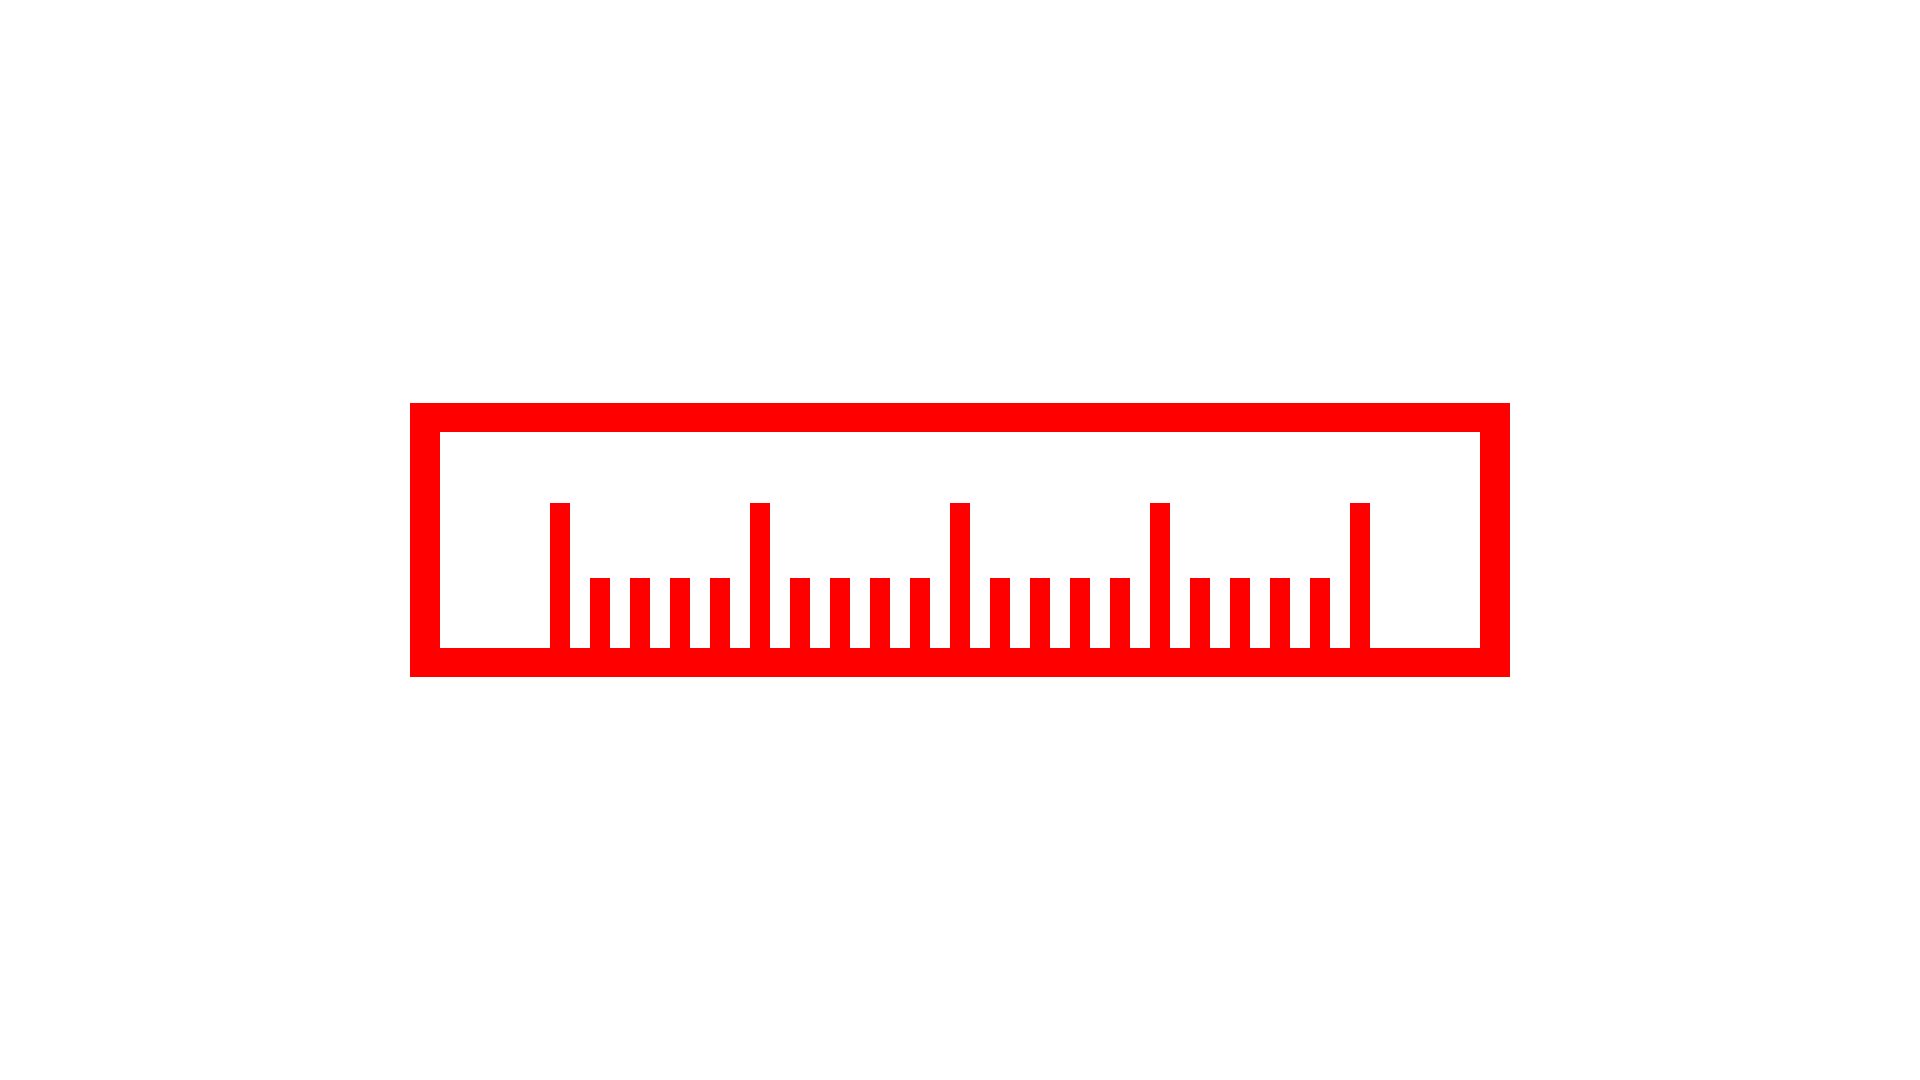
\includegraphics[scale=0.1]{ruler}};


\draw[dotted] (2.95, -0.2) -- (2.95,2);
\node[black] (russell) at (2.95,-0.2) {$x_1$};

\draw[dotted] (3.7, -0.2) -- (3.7,2);
\node[black] (russell) at (3.7,-0.2) {$x_2$};


%\draw[axis, black] (3.7, 2) -- (4.7, 2) node[midway, above] {$v$};

% --- distancia entre sistemas ---
\draw[axis, gray] (3.15, 0.5) -- (2.95, 0.5) node[midway, ,gray,pos=-0.8] {$t$};
\draw[axis, gray] (3.5, 0.5) -- (3.7, 0.5);



\end{tikzpicture}
%\end{center}
% --- Fin del código TikZ ---
    \caption{Sistema de referencia inercial $\color{red}S'$, moviendos con velocidad constante en $x$, $v$, con el objeto bajo estudio }
    \label{fig:movruler}
\end{figure}




La contracción de la longitud es otra predicción fundamental de la Relatividad Especial. Afirma que se mide que un objeto en movimiento es más corto a lo largo de su dirección de movimiento que su longitud cuando se mide en reposo. Este efecto también se conoce como contracción de Lorentz.

La clave para medir correctamente la longitud de un objeto en movimiento es determinar las posiciones de sus dos extremos \textbf{simultáneamente} en el sistema de referencia del observador.

\subsection{Definición de la longitud propia}
La longitud propia, $L_0$, es la distancia entre dos puntos cuyas posiciones son medidas por un observador en reposo respecto a los dos puntos. Por definición, el observador en el sistema de referencia en reposo, por definición, mide distancias propias a todos los objetos en reposo con respecto a él, como la distancia a un florero sobre la mesa de la habitación en la que se encuentra. Lo mismo aplica para el observador en movimiento en el sistema $S'$: la distancia a objetos en reposo relativo a él son distancias propias para él, como la distancia al monitor de la pantalla dentro de su nave espacial. De esta forma, la longitud de la cancha de tenis es una distancia propia para un tenista en reposo que golpea fuertemente una pelota de tenis. El diámetro de la pelota de tenis es, a su vez, una distancia propia para una hormiga pegada a la bola de tenis en movimiento. Por lo tanto, el tenista verá la pelota de tenis contraída en su dirección de movimiento y la hormiga percibirá que la cancha de tenis tiene una longitud menor a la que percibe el tenista. 

% --- Inicio del código LaTeX para insertar ---

\subsection*{Demostración de la Contracción de Lorentz a partir de la Dilatación del Tiempo}

Esta es una de las demostraciones más elegantes en relatividad, ya que muestra cuán profundamente entrelazados están el espacio y el tiempo. En lugar de derivar la contracción de la longitud directamente de los postulados, la derivaremos como una consecuencia lógica de la dilatación del tiempo. Para ello, construiremos un experimento mental que involucre tanto una medición de distancia como una de tiempo desde dos perspectivas diferentes.

\subsection*{El Experimento Mental}
Imaginemos un viaje espacial:
\begin{itemize}
    \item Hay dos puntos fijos en el espacio: un punto de partida (la Tierra) y un punto de destino (una estrella lejana).
    \item Un observador en la Tierra (en el sistema de referencia \textbf{S}) mide la distancia entre la Tierra y la estrella. Como esta distancia está en reposo con respecto a él, mide la \textbf{longitud propia}, $L_0$.
    \item Una nave espacial (en el sistema de referencia \textbf{S'}) viaja de la Tierra a la estrella a una velocidad constante $v$.
\end{itemize}
Nuestro objetivo es encontrar la distancia entre la Tierra y la estrella medida por el astronauta en la nave, a la que llamaremos $L$.

\subsection*{La Demostración: Paso a Paso}
La demostración se basa en calcular el tiempo del viaje desde ambas perspectivas y luego conectarlos usando la fórmula de la dilatación del tiempo.

\subsubsection*{Paso 1: La Perspectiva de la Tierra (Sistema S)}
\begin{itemize}
    \item \textbf{Distancia del viaje:} Para el observador en la Tierra, la distancia que debe recorrer la nave es la longitud propia, $L_0$.
    \item \textbf{Tiempo del viaje:} El observador en la Tierra mide el tiempo que tarda la nave en completar el viaje usando sus propios relojes. Llamaremos a este tiempo $\Delta t$. Usando la fórmula básica \texttt{tiempo = distancia / velocidad}, tenemos:
    \[ \Delta t = \frac{L_0}{v} \]
\end{itemize}
Despejando la distancia, obtenemos nuestra primera ecuación clave:
\begin{equation} \label{eq:dist_tierra}
    L_0 = v \cdot \Delta t
\end{equation}

\subsubsection*{Paso 2: La Perspectiva del Astronauta (Sistema S')}
\begin{itemize}
    \item \textbf{Distancia del viaje:} Para el astronauta, él está en reposo y es la estrella la que se acerca a él a una velocidad $v$. La distancia que él mide entre la Tierra y la estrella es $L$.
    \item \textbf{Tiempo del viaje:} El astronauta mide la duración del viaje en su propio reloj. Este tiempo es el \textbf{tiempo propio}, $\Delta t_0$, porque para él, los eventos de ``salida'' y ``llegada'' ocurren en su misma ubicación (en $x'=0$). De nuevo, usando \texttt{tiempo = distancia / velocidad}:
    \[ \Delta t_0 = \frac{L}{v} \]
\end{itemize}
Despejando la distancia, obtenemos nuestra segunda ecuación clave:
\begin{equation} \label{eq:dist_nave}
    L = v \cdot \Delta t_0
\end{equation}

\subsubsection*{Paso 3: El Puente - Conectando las Perspectivas con la Dilatación del Tiempo}
Ahora tenemos dos ecuaciones diferentes para la distancia, cada una involucrando una medida de tiempo diferente. Aquí es donde entra en juego la \textbf{dilatación del tiempo}, que actúa como un puente entre los dos sistemas de referencia.

La fórmula de la dilatación del tiempo nos dice cómo se relacionan el tiempo medido por el observador en la Tierra ($\Delta t$) y el tiempo propio medido por el astronauta ($\Delta t_0$):
\begin{equation} \label{eq:dilatacion}
    \Delta t = \gamma \Delta t_0 \quad \text{donde} \quad \gamma = \frac{1}{\sqrt{1 - v^2/c^2}}
\end{equation}

\subsubsection*{Paso 4: Combinar las Ecuaciones y Resolver}
Tenemos un sistema de tres ecuaciones y nuestro objetivo es encontrar una relación entre $L$ y $L_0$.
\begin{enumerate}
    \item Partimos de la Ecuación (\ref{eq:dist_tierra}):
    \[ L_0 = v \cdot \Delta t \]
    \item Sustituimos la Ecuación (\ref{eq:dilatacion}) en la ecuación anterior para eliminar $\Delta t$:
    \[ L_0 = v \cdot (\gamma \Delta t_0) \]
    \item Ahora, observamos la Ecuación (\ref{eq:dist_nave}), que nos dice que $L = v \cdot \Delta t_0$. Podemos sustituir todo el término $(v \cdot \Delta t_0)$ en nuestra ecuación actual por $L$:
    \[ L_0 = \gamma (v \cdot \Delta t_0) \implies L_0 = \gamma L \]
\end{enumerate}
Finalmente, despejamos $L$, la longitud medida por el astronauta en movimiento:
\[ L = \frac{L_0}{\gamma} \]

\subsection*{Resultado y Conclusión}
Al sustituir la expresión completa para $\gamma$, obtenemos la fórmula de la contracción de la longitud:
\[ \boxed{ L = L_0 \sqrt{1 - v^2/c^2} } \]
Hemos demostrado con éxito que la contracción de la longitud es una consecuencia directa y necesaria de la dilatación del tiempo. Al insistir en que ambos observadores deben estar de acuerdo en los hechos básicos, inevitablemente llegamos a la conclusión de que para el objeto en movimiento la distancia del viaje es más corta. Esto subraya que el espacio y el tiempo están intrínsecamente entrelazados.

% --- Fin del código LaTeX ---

ver \url{https://inspirehep.net/literature/2825885}

\subsection{Perspectiva Histórica: El Experimento de Michelson-Morley y la Naturaleza de la Contracción}

La derivación de la contracción de la longitud suele generar una profunda inquietud conceptual en los estudiantes: ¿Se ``aplastan'' los objetos físicamente o es solo una ilusión óptica? Para aclarar esta diferencia, es fundamental revisar el experimento más famoso que falló en la historia de la física: el experimento de Michelson y Morley (1887).

A finales del siglo XIX, los físicos estaban convencidos de que las ondas electromagnéticas (la luz) requerían un medio material para propagarse, al igual que el sonido requiere aire. A este medio invisible, estacionario y que llenaba todo el universo, se le llamó el \textbf{éter luminífero}. El experimento de Michelson y Morley fue diseñado para medir la velocidad de la Tierra a través de este éter.

\begin{figure}[h]
    \centering
    \begin{tikzpicture}[>=stealth, scale=1.5]
    
        % --- ESTILOS ---
        \tikzstyle{mirror}=[draw, thick, fill=gray!30, minimum width=2pt, minimum height=30pt, inner sep=0pt]
        \tikzstyle{splitter}=[draw, thick, fill=cyan!20, minimum width=2pt, minimum height=35pt, inner sep=0pt, rotate=45]
        \tikzstyle{beam}=[thick, ->]
        
        % --- COMPONENTES ---
        % Fuente de luz
        \node[draw, thick, fill=yellow!20, minimum size=20pt, align=center] (Source) at (-2.5, 0) {Fuente};
        
        % Divisor de haz (Espejo semitransparente)
        \node[splitter] (Splitter) at (0, 0) {};
        \node[below left, xshift=-5pt, yshift=-5pt] at (0,0) {Divisor};
    
        % Espejo 1 (Brazo paralelo al movimiento)
        \node[mirror] (M1) at (2.5, 0) {};
        \node[right] at (2.6, 0) {Espejo 1};
        \draw[<->, gray] (0,-0.5) -- (2.5,-0.5) node[midway, below] {$L_\parallel$};
    
        % Espejo 2 (Brazo perpendicular al movimiento)
        \node[mirror, rotate=90] (M2) at (0, 2.5) {};
        \node[above] at (0, 2.6) {Espejo 2};
        \draw[<->, gray] (-0.5,0) -- (-0.5,2.5) node[midway, left] {$L_\perp$};
    
        % Detector
        \node[draw, thick, fill=green!20, minimum width=30pt, minimum height=15pt, align=center] (Detector) at (0, -2.5) {Detector};
    
        % --- RAYOS DE LUZ ---
        % Haz incidente
        \draw[beam, red] (Source.east) -- (-0.1, 0);
        
        % Brazo 1 (Ida y vuelta)
        \draw[beam, red, transform canvas={yshift=2pt}] (0.1, 0) -- (2.4, 0);
        \draw[beam, red, transform canvas={yshift=-2pt}] (2.4, 0) -- (0.1, 0);
    
        % Brazo 2 (Ida y vuelta)
        \draw[beam, blue, transform canvas={xshift=2pt}] (0, 0.1) -- (0, 2.4);
        \draw[beam, blue, transform canvas={xshift=-2pt}] (0, 2.4) -- (0, 0.1);
    
        % Haz recombinado al detector
        \draw[beam, purple, line width=1.5pt] (0, -0.1) -- (Detector.north);
    
        % --- MOVIMIENTO DE LA TIERRA ---
        \draw[->, ultra thick, orange!90!black] (1.5, 1.5) -- (3, 1.5) node[midway, above] {$\boldsymbol{v}$ (Tierra)};
    
    \end{tikzpicture}
    \caption{Esquema simplificado del Interferómetro de Michelson-Morley. Un haz de luz se divide en dos: uno viaja paralelo al movimiento de la Tierra ($L_\parallel$) y otro perpendicular ($L_\perp$). Al recombinarse en el detector, cualquier diferencia en el tiempo de viaje produciría un patrón de interferencia.}
    \label{fig:michelson_morley}
\end{figure}

El montaje experimental, mostrado en la Figura \ref{fig:michelson_morley}, divide un haz de luz en dos brazos. Si la Tierra navega por el éter a velocidad $v$, la luz que viaja en el brazo paralelo ($L_\parallel$) debe luchar contra el ``viento de éter'', retrasándose respecto a la luz que viaja por el brazo perpendicular ($L_\perp$). Asombrosamente, el resultado fue nulo: ambos haces llegaban siempre al mismo tiempo, sin importar en qué época del año o en qué dirección apuntara el aparato.

\subsubsection*{La Interpretación Dinámica: El Éter y la Contracción ``Real''}

Para salvar la idea del éter ante este resultado negativo, los físicos George FitzGerald (en 1889) y Hendrik Lorentz (en 1892) propusieron una explicación audaz. Argumentaron que si un objeto físico se mueve a través del éter, la presión o interacción mecánica de esta sustancia con las fuerzas electromagnéticas que unen los átomos provocaría que el objeto se \textit{comprimiera físicamente} en la dirección del movimiento en un factor exacto de $\sqrt{1 - v^2/c^2}$.

Bajo esta interpretación, si preguntamos \textit{¿qué tipo de observador vería el brazo del interferómetro contraído?}, la respuesta es clara: \textbf{solo un observador hipotético que se encuentre en reposo absoluto con respecto al éter}. 

Este observador estacionario vería pasar a la Tierra y notaría que el brazo $L_\parallel$ del interferómetro se acortó de verdad. Sin embargo, el experimentador en la Tierra no notaría nada. Si intentara medir el brazo con una regla de madera, la regla misma se habría contraído mecánicamente por el éter en la misma proporción. 

Al hacerse físicamente más corto el brazo $L_\parallel$, la luz recorre menos distancia. Este ahorro de distancia compensa con una exactitud milimétrica el retraso sufrido al nadar contra el viento de éter, explicando perfectamente el resultado nulo del experimento. En este paradigma, la contracción es absoluta y asimétrica.

\subsubsection*{La Interpretación Cinemática: Relatividad Especial}

En 1905, Albert Einstein revolucionó la física al proponer una solución radicalmente distinta. Einstein descartó el éter por completo, considerándolo indetectable e innecesario. En su lugar, postuló que la velocidad de la luz, $c$, es exactamente la misma para todos los observadores inerciales, independientemente de la velocidad de la fuente.

En la Relatividad Especial, la contracción de la longitud que derivamos en la sección anterior no es una deformación mecánica, estructural o física provocada por la fricción contra un fluido estelar. Es, por el contrario, un \textbf{efecto cinemático relativo} derivado de la geometría misma del espaciotiempo. 

Como el espacio y el tiempo están entrelazados, la longitud de un objeto se define localizando sus dos extremos \textit{simultáneamente}. Pero la relatividad demuestra que la simultaneidad es relativa: dos eventos que son simultáneos para el experimentador en la Tierra no lo son para un observador que pasa volando en una nave. Al diferir en su medición del tiempo, difieren necesariamente en su medición del espacio.

La gran diferencia entre la contracción de Lorentz (éter) y la de Einstein (relatividad) es la \textbf{simetría}. En la teoría del éter, solo el objeto que se mueve a través del fluido absoluto se acorta. En la teoría de Einstein, no hay movimiento absoluto: si tú viajas en una nave y yo me quedo en la Tierra, yo mido que tu nave está contraída, pero tú observas que soy yo y mi planeta los que estamos contraídos en la dirección de tu movimiento. La contracción relativista es un efecto de perspectiva espaciotemporal, no un colapso material.

\section{Suma de velocidades relativista}

En la física clásica (galileana), si estás en un tren que se mueve a una velocidad $v$, y lanzas una pelota hacia adelante a una velocidad $u'$ (relativa al tren), un observador en el suelo vería la pelota moverse a una simple suma de las velocidades:
\[ u = u' + v \quad \text{(Suma Clásica/Galileana)} \]
Esto funciona perfectamente a velocidades cotidianas. Sin embargo, se rompe a velocidades relativistas.

\textbf{La Contradicción:} Imagina una nave espacial (sistema $S'$) que se aleja de la Tierra (sistema $S$) a $v=0.8c$. La nave dispara una sonda hacia adelante a una velocidad de $u'=0.7c$ relativa a sí misma. Según la fórmula clásica, un observador en la Tierra vería la sonda moverse a:
\[ u = 0.7c + 0.8c = 1.5c \]
Esto es más rápido que la velocidad de la luz, lo cual viola el segundo postulado de la Relatividad Especial. Necesitamos una nueva fórmula que respete el límite de velocidad cósmico.

\subsubsection*{La Configuración para la Fórmula Relativista}

Usamos tres sistemas de referencia:
\begin{itemize}
    \item \textbf{Sistema S:} Un observador estacionario (por ejemplo, en la Tierra).
    \item \textbf{Sistema S':} Un sistema que se mueve con velocidad $v$ relativa a $S$ (por ejemplo, la nave espacial).
    \item \textbf{Objeto:} Un objeto que se mueve con velocidad $u'$ relativa a $S'$.
\end{itemize}
Nuestro objetivo es encontrar la velocidad del objeto, \textbf{$u$}, medida por el observador en el sistema estacionario, $S$.
\[
\text{S (Tierra)} \quad \xrightarrow{v} \quad \text{S' (Nave)} \quad \xrightarrow{u'} \quad \text{Objeto (Sonda)}
\]
\[
\text{¿Cuál es la velocidad } u \text{ del Objeto relativa a S?}
\]

\subsection{Derivación a partir de las Transformaciones de Lorentz}

Las velocidades constantes se definen como el cociente entre la posición y el tiempo:
\[ u = \frac{x}{t} \quad \text{y} \quad u' = \frac{x'}{t'}\,, \]
que son respectivamente las velocidades del un objeto con respecto a los sistemas $S$ y $S'$ que se me mueve a su vez con una velocidad $v$

Comenzamos con las transformaciones de Lorentz que relacionan las coordenadas:
\begin{align*}
x' &= \gamma(x - vt) \\
t' &= \gamma\left(t - \frac{vx}{c^2}\right)
\end{align*}
Ahora, podemos construir la fracción para $u'$ dividiendo $x'$ por $t'$:
\[ u' = \frac{x'}{t'} = \frac{\gamma(x - vt)}{\gamma\left(t - \dfrac{v\,x}{c^2}\right)} \]
Los factores $\gamma$ se cancelan:
\[ u' = \frac{x - v\,t}{t - \dfrac{v\,x}{c^2}} \]
Para poner esto en términos de velocidades, dividimos el numerador y el denominador por $dt$:
\[ u' = \frac{\dfrac{x}{t} - v\dfrac{t}{t}}{\dfrac{t}{t} - \dfrac{v}{c^2}\dfrac{x}{t}} \]
Sustituyendo $u = {x}/{t}$:
\[ u' = \frac{u - v}{1 - \dfrac{uv}{c^2}} \]
Esta fórmula da la velocidad relativa $u'$ cuando conoces las velocidades en el sistema estacionario. Sin embargo, queremos ``sumar" velocidades, lo que significa que necesitamos resolver esta ecuación para $u$.

\noindent
\setcounter{paso}{0}
\begin{tabular}{l|p{0.35\textwidth}|p{0.6\textwidth}}
\textbf{paso} &\textbf{Despejar} $u$& \textbf{Paso algebraico} \\\hline
\stepcounter{paso}\thepaso) & $ u' = \dfrac{u - v}{1 - \frac{uv}{c^2}} $
 & Ecuación inicial \\[5pt]\hline
\stepcounter{paso}\thepaso) & $u'\left(1 - \dfrac{uv}{c^2}\right) = u - v $ & Multiplicar por $\left(1 - \dfrac{uv}{c^2}\right)$ a ambos lados de la igualdad \\[5pt]\hline
\stepcounter{paso}\thepaso) & $u' - \dfrac{u'uv}{c^2} = u - v$ & Distribuir $u'$ en el lado derecho.\\[5pt]\hline
\stepcounter{paso}\thepaso) & $u' + v = u + \dfrac{u'uv}{c^2}$ & Reunir términos con $u$. \\[5pt]\hline
\stepcounter{paso}\thepaso) & $u' + v = u\left(1 + \dfrac{u'v}{c^2}\right)$ & Factorizar $u$. \\[5pt]\hline
\stepcounter{paso}\thepaso) & $u = \dfrac{u' + v}{1 + \frac{u'v}{c^2}}$& Dividiendo por $\left(1 + \dfrac{u'v}{c^2}\right)$ a ambos lados de la igualdad.\\[7pt]\hline

\end{tabular}


De esta forma obtenemos da la \textbf{Fórmula de Suma de Velocidades de Einstein}:
\[
\boxed{
u = \frac{u' + v}{1 + \dfrac{u'v}{c^2}}
}
\]

\subsection*{Ejercicio: Despejar $c^2$ de la fórmula de suma de velocidades}
\noindent
\setcounter{paso}{0}
\begin{tabular}{l|p{0.3\textwidth}|p{0.65\textwidth}}
\textbf{paso} &\textbf{Despejar} $c^2$& \textbf{Paso algebraico} \\\hline
\stepcounter{paso}\thepaso) & $u = \dfrac{u' + v}{1 + \frac{u'v}{c^2}}$& Ecuación inicial\\[7pt]\hline
\stepcounter{paso}\thepaso) & $u\left(1 + \dfrac{u'v}{c^2}\right) = u' + v $ & Multiplicar por $\left(1 + \dfrac{u'v}{c^2}\right)$ a ambos lados de la igualdad. \\[5pt]\hline
\stepcounter{paso}\thepaso) & \phantom{$u + \dfrac{u u'v}{c^2} =  u' + v$}& Distribuir $u$ en el lado derecho.\\[5pt]\hline
\stepcounter{paso}\thepaso) & $\dfrac{u u'v}{c^2} =  u' + v - u$& \phantom{Restar $u$ a ambos lados de la igualdad.}\\[5pt]\hline
\stepcounter{paso}\thepaso) &\phantom{ $\dfrac{c^2}{u u'v} = \dfrac{1}{ u' + v - u}$}& Tomar el reciproco a ambos lados de la igualdad.\\[5pt]\hline
\stepcounter{paso}\thepaso) & $c^2 = \dfrac{u u'v}{ u' + v - u}$ & \phantom{ Multiplicar por $u u'v$ a ambos lados de la igualdad. }\\[5pt]\hline
\end{tabular}

El resultado de despejar $c^2$ es entonces

\begin{align}
\boxed{
    c^2 = \dfrac{u u'v}{ u' + v - u}
    \,.}
\end{align}

En el límite no relativista de $u\approx u'+v$, tenemos que
\begin{align}
    c^2 = \dfrac{u u'v}{ u' + v - u} \approx \dfrac{(u'+v) u'v}{0} = \infty\,, 
\end{align}
tenemos que  $c = \infty$ y de éste modo en el límite no relativista, ¡no existe una velocidad límite!.




\subsection{Ejemplos}

\subsection*{Ejemplo 1: La Nave Espacial y la Sonda}
Volvamos a nuestro problema inicial con la fórmula relativista.
\begin{itemize}
    \item $v = 0.8c$ (velocidad de la nave relativa a la Tierra)
    \item $u' = 0.7c$ (velocidad de la sonda relativa a la nave)
\end{itemize}
\[ u = \frac{0.7c + 0.8c}{1 + \frac{(0.7c)(0.8c)}{c^2}} = \frac{1.5c}{1 + \frac{0.56c^2}{c^2}} = \frac{1.5c}{1 + 0.56} = \frac{1.5c}{1.56} \]
\[ u \approx 0.9615c \]
El resultado es menor que la velocidad de la luz, como se requiere.

\subsection*{Característica 1: La Velocidad de la Luz es el Límite Último}
¿Qué pasa si la nave que se mueve a $v=0.9c$ dispara un rayo láser hacia adelante ($u'=c$)?
\[ u = \frac{c + 0.9c}{1 + \frac{(c)(0.9c)}{c^2}} = \frac{1.9c}{1 + 0.9} = \frac{1.9c}{1.9} = c \]
El observador en la Tierra también mide la velocidad del rayo láser como exactamente $c$. Este hermoso resultado muestra cómo la fórmula defiende perfectamente el segundo postulado de la relatividad. 

\subsection*{Característica 2: Se Reduce a la Fórmula Clásica a Bajas Velocidades}
Si $v \ll c$ y $u' \ll c$, el término $\frac{u'v}{c^2}$ se vuelve extremadamente pequeño y se aproxima a cero.
\[ u = \frac{u' + v}{1 + \frac{u'v}{c^2}} \approx \frac{u' + v}{1} = u' + v \]
Esto muestra que la fórmula relativista contiene la fórmula clásica como una aproximación a baja velocidad, lo cual es un requisito clave para cualquier nueva teoría física.

\section{Propagación de ondas y efecto Doppler}



\subsection{Adición de velocidades no relativistas para ondas mecánicas}



Una pregunta fundamental al estudiar cinemática y ondas es si la velocidad de propagación de una onda depende de la velocidad del observador en un sistema de referencia inercial. En el caso del sonido, la respuesta es afirmativa, mientras que para la luz revela la necesidad de un cambio radical en nuestra comprensión del universo.

\subsubsection{El Aire como un Sistema de Referencia Privilegiado}

El sonido no puede viajar en el vacío; requiere un medio material (como el aire, el agua o un metal) para propagarse. La velocidad del sonido, que denotaremos como $c_s$ (aproximadamente $343 \text{ m/s}$ en el aire a temperatura ambiente), es constante \textbf{únicamente con respecto a ese medio material}.

Dado que aplica la relatividad de Galileo (la suma clásica de velocidades), si un observador se mueve con una velocidad $v$ con respecto al aire, la velocidad de la onda de sonido con respecto al sistema de movimiento ($c'_s$) es:
\begin{itemize}
    \item \textbf{Si el observador se acerca a la fuente:} $c'_s$ es mayor,
    \begin{equation}
       c'_s = c_s + v.
    \end{equation}
    \item \textbf{Si el observador se aleja de la fuente:} La velocidad percibida es menor,
    \begin{equation}
        c'_s = c_s - v.
    \end{equation}
\end{itemize}

Para las ondas mecánicas como el sonido, el medio material (el aire) actúa como un sistema de referencia privilegiado o absoluto. Cualquier observador inercial que se mueva a través de él medirá una velocidad de propagación diferente.

\subsection{El Espejismo del Éter y el Experimento de Michelson-Morley}

Durante el siglo XIX, los físicos asumieron en su contexto histórico que la luz debía comportarse exactamente igual que el sonido. Si el sonido necesitaba el aire, razonaban que las ondas electromagnéticas (la luz) debían necesitar un medio elástico invisible que llenara todo el universo, al cual denominaron el \textbf{éter luminífero}. 

Bajo esta suposición, el éter constituía el ``sistema de referencia absoluto'' del cosmos. Los científicos creían que la Tierra, al orbitar alrededor del Sol, se movía a través de este éter, generando un ``viento de éter'' detectable. 

Sin embargo, como revisamos en nuestra perspectiva histórica, el célebre \textbf{experimento de Michelson-Morley (1887)} midió la velocidad de la luz en direcciones perpendiculares y descubrió un resultado totalmente nulo: la velocidad de la luz era exactamente la misma en todas las direcciones, sin importar el movimiento de la Tierra. 

\subsubsection{La Solución de Einstein: La Ausencia de Medio}

La gran revelación que condujo a la Relatividad Especial fue entender por qué el experimento de Michelson-Morley falló: \textbf{el éter no existe}. 

\begin{itemize}
    \item \textbf{El Sonido} depende de un medio material (el aire), lo que crea un marco de referencia absoluto y genera asimetrías en la velocidad percibida.
    \item \textbf{La Luz} es una perturbación de campos electromagnéticos que \textbf{no requiere ningún medio material} para propagarse. 
\end{itemize}

Al no existir un medio de referencia absoluto ni un ``éter'' que sirva de anclaje, la naturaleza no tiene cómo distinguir qué observador está ``realmente en reposo'' y cuál está en movimiento. Esto elevó la velocidad de la luz ($c$) a una constante universal e invariante para todos los observadores inerciales, \textbf{revelando los límites de validez de la física galileana y ampliando el marco conceptual hacia las transformaciones de Lorentz}, unificando así el electromagnetismo bajo un nuevo estándar geométrico que contiene a la mecánica clásica como un caso límite a bajas velocidades.

\subsection*{Consecuencia: El Efecto Doppler Clásico}

Esta dependencia de la velocidad relativa es la razón física subyacente por la cual experimentamos el \textbf{Efecto Doppler} en la acústica. 




\subsection{Deducción Algebraica del Efecto Doppler para el Sonido}

El Efecto Doppler describe el cambio en la frecuencia percibida de una onda cuando existe movimiento relativo entre la fuente emisora y el observador. A diferencia de la luz, el sonido requiere un medio material (el aire), por lo que las velocidades de la fuente y del observador se miden siempre respecto a dicho medio (asumido en reposo).

Definiremos las siguientes variables:
\begin{itemize}
    \item $f_0$: Frecuencia emitida por la fuente.
    \item $v_s$: Velocidad del sonido en el aire.
    \item $v_f$: Velocidad de la fuente.
    \item $v_o$: Velocidad del observador.
    \item $\lambda_0$: Longitud de onda original ($\lambda_0 = v_s / f_0$).
\end{itemize}

\subsubsection{1. El Movimiento de la Fuente (Efecto en la Longitud de Onda)}

Imaginemos que la fuente se mueve a una velocidad $v_f$ hacia un observador que está quieto ($v_o = 0$). En un segundo, la fuente emite $f_0$ ondas. Durante ese intervalo de tiempo de $1 \text{ s}$, la primera onda emitida avanza una distancia de $v_s \cdot (1 \text{ s})$ a través del aire, mientras que la fuente se ha desplazado una distancia $v_f \cdot (1 \text{ s})$ en la misma dirección, persiguiendo a su propia onda y comprimiendo el espacio entre los frentes de onda subsiguientes.

Algebraicamente, la nueva longitud de onda comprimida ($\lambda'$), vista en la Ecuación (\ref{eq:doppler_longitud_onda}), es:
\begin{equation}
    \lambda' = \frac{v_s - v_f}{f_0}.
    \label{eq:doppler_longitud_onda}
\end{equation}
\textit{(Nota: Si la fuente se alejara, el espacio se estiraría, cambiando el signo a $v_s + v_f$).}

Como el observador está en reposo respecto al aire, estas ondas comprimidas viajan hacia él a la velocidad normal del sonido $v_s$. La frecuencia percibida ($f_{\text{obs}}$) es la velocidad de la onda dividida entre esta nueva longitud de onda:
\begin{equation}
    f_{\text{obs}} = \frac{v_s}{\lambda'} = \frac{v_s}{\left(\frac{v_s - v_f}{f_0}\right)}.
\end{equation}

Reorganizando mediante división de fracciones, obtenemos la fórmula cuando la fuente está en movimiento y el observador en reposo:
\begin{equation}
    f_{\text{obs}} = f_0 \left( \frac{v_s}{v_s \mp v_f} \right),
    \label{eq:doppler_fuente}
\end{equation}
donde se usa el signo menos ($-$) si la fuente se acerca, y el signo más ($+$) si la fuente se aleja.

\subsubsection{2. El Movimiento del Observador (Efecto en la Velocidad Relativa)}

Imaginemos ahora que la fuente está inmóvil ($v_f = 0$), pero es el observador quien se mueve a una velocidad $v_o$. 

Las ondas viajan por el aire a $v_s$. Si el observador se mueve al encuentro de las ondas, la velocidad relativa de impacto ya no es solo $v_s$, sino que se le suma su propia velocidad ($v_s + v_o$). Si huye, la velocidad relativa disminuye ($v_s - v_o$).

La frecuencia percibida se calcula dividiendo esta nueva velocidad de impacto entre la longitud de onda original $\lambda_0$:
\begin{equation}
    f_{\text{obs}} = \frac{v_s \pm v_o}{\lambda_0} = \frac{v_s \pm v_o}{\left(\frac{v_s}{f_0}\right)} = f_0 \left( \frac{v_s \pm v_o}{v_s} \right).
\end{equation}

Reorganizando, obtenemos la fórmula cuando el observador está en movimiento y la fuente en reposo:
\begin{equation}
    f_{\text{obs}} = f_0 \left( \frac{v_s \pm v_o}{v_s} \right),
    \label{eq:doppler_observador}
\end{equation}
donde se usa el signo más ($+$) si el observador se acerca, y menos ($-$) si se aleja.


En resumen, para las ondas mecánicas como el sonido, el medio material (el aire) actúa como un sistema de referencia privilegiado. Cualquier observador inercial que se mueva a través de él medirá una velocidad de propagación diferente. Esta profunda asimetría en la física clásica servirá de contraste vital para entender el comportamiento de la luz, la cual no requiere de un medio para propagarse y mantiene su velocidad invariable sin importar quién la mida.


\subsection*{El Efecto Doppler: Sonido Clásico vs. Luz Relativista}

El efecto Doppler es el fenómeno por el cual la frecuencia percibida de una onda cambia cuando la fuente y el observador se encuentran en movimiento relativo. Sin embargo, existe una diferencia fundamental entre las ondas mecánicas (como el sonido) que requieren un medio material, y las ondas electromagnéticas (como la luz) cuya velocidad es invariante.

\subsubsection*{Derivación del Efecto Doppler Relativista (Fuente Alejándose)}

A diferencia del sonido, donde usamos las transformaciones de Galileo, para la luz debemos usar la Relatividad Especial. Deduciremos la fórmula para una fuente (como una nave espacial) que se aleja de un observador en la Tierra con una velocidad $v$.

\textbf{Paso 1: El tiempo propio.} En el sistema de referencia de la nave, el tiempo que transcurre entre la emisión de un pulso de luz y el siguiente es el periodo propio, $T_0$. Su frecuencia original es
\begin{equation}
    f_0 = \frac{1}{T_0}.
\end{equation}

\textbf{Paso 2: Dilatación del tiempo.} Desde la Tierra, vemos que el reloj de la nave funciona más lentamente debido a la relatividad. El tiempo dilatado $T$ medido por nosotros entre las emisiones de los pulsos es
\begin{equation}
    T = \gamma T_0 = \frac{T_0}{\sqrt{1 - \beta^2}}\,,
\end{equation}
con $\beta=v/c$ (ver ec.~\ref{eq:beta}).

\textbf{Paso 3: El estiramiento geométrico.} Mientras la nave espera ese tiempo dilatado $T$ para emitir el segundo pulso, sigue alejándose de nosotros, recorriendo una distancia adicional $d = v T$. El tiempo extra de viaje que debe recorrer el segundo pulso para alcanzarnos es
\begin{equation}
    t_{\text{extra}} = \frac{d}{c} = \frac{v T}{c}.
\end{equation}

\textbf{Paso 4: El periodo observado.} El tiempo total medido en la Tierra entre la llegada del primer y segundo pulso, $T_{\text{obs}}$, será el tiempo dilatado $T$ más el tiempo extra de viaje:
\begin{equation}
    T_{\text{obs}} = T + \frac{v T}{c} = T \left(1 + \frac{v}{c}\right),
\end{equation}
de modo que
\begin{equation}
\label{eq:tobs0}
    T_{\text{obs}} =  T_0\gamma \left(1 + \frac{v}{c}\right).
\end{equation}


\textbf{Paso 5: Álgebra y simplificación.} Sustituimos el tiempo dilatado $T$ del Paso 2 en la ecuación anterior:
\begin{equation}
    T_{\text{obs}} = \frac{T_0}{\sqrt{1 - \frac{v^2}{c^2}}} \left(1 + \frac{v}{c}\right).
\end{equation}
Aplicamos la diferencia de cuadrados en el denominador, $\left(1 - \frac{v^2}{c^2}\right) = \left(1 - \frac{v}{c}\right)\left(1 + \frac{v}{c}\right)$, y reescribimos el numerador como $\sqrt{1 + \frac{v}{c}} \sqrt{1 + \frac{v}{c}}$:
\begin{equation}
    T_{\text{obs}} = T_0 \frac{\sqrt{1 + \dfrac{v}{c}} \cancel{\sqrt{1 + \dfrac{v}{c}}}}{\sqrt{1 - \dfrac{v}{c}}\cancel{ \sqrt{1 + \dfrac{v}{c}}}}.
\end{equation}
Al cancelar términos semejantes, obtenemos el periodo observado:
\begin{equation}
    T_{\text{obs}} = T_0 \sqrt{\frac{1 + \beta}{1 - \beta}}\,,
\end{equation}
donde $\beta=v/c$ (ver ec.~\eqref{eq:beta}.

Note que hemos usado la identidad:
\begin{equation}
\label{eq:doppid}
 \sqrt{\frac{1+\beta}{1-\beta}} =   \gamma (1+\beta).
\end{equation}


\textbf{Paso 6: La frecuencia observada.} La frecuencia observada ($f_{\text{obs}}$) es la inversa del periodo ($1 / T_{\text{obs}}$). Al invertir la fracción dentro de la raíz, obtenemos la fórmula del \textbf{Efecto Doppler Relativista} para una fuente que se aleja (lo que explica el corrimiento al rojo o \textit{redshift} de las galaxias):
\begin{equation}
    f_{\text{obs}} = f_0 \sqrt{\frac{1 - \beta}{1 + \beta}},,
    \label{eq:doppler_aleja}
\end{equation}
\textit{Nota:} Si la fuente y el observador se estuvieran \textbf{acercando}, simplemente invertimos los signos de la ecuación (\ref{eq:doppler_aleja}), obteniendo un corrimiento hacia el azul (mayor frecuencia).

De esta forma, si la frecuencia inicial de la fuente se conoce, a pesar de que la \emph{velocidad de la luz no cambia} si la fuente se acerca o se aleja con respecto al observador; \emph{la frecuencia medida por dicho observador si cambia}, desplazándose hacía el azul o el rojo respectivamente.

\subsection{Ejemplos}

\subsubsection{Invarianza con respecto a sistemas de referencia}
Suponga que un observador está sobre una plataforma abierta al aire que se mueve sobre una vía férrea a una velocidad constante  $v$. El observador está sentado mirando hacía el frente en la dirección de movimiento. Un músico está sentado a un metro frente al observador dando la espalada a la dirección de movimiento. Sí el músico dirige una nota ``Do'' hacia el observador ¿a qué velocidad se mueve esa onda hacia el observador y a que frecuencia es percibida por el observador?. Repetir el análisis para el caso de un rayo laser verde como se muestra en la figura~\ref{fig:sl}

\begin{figure}[H]
    \centering
    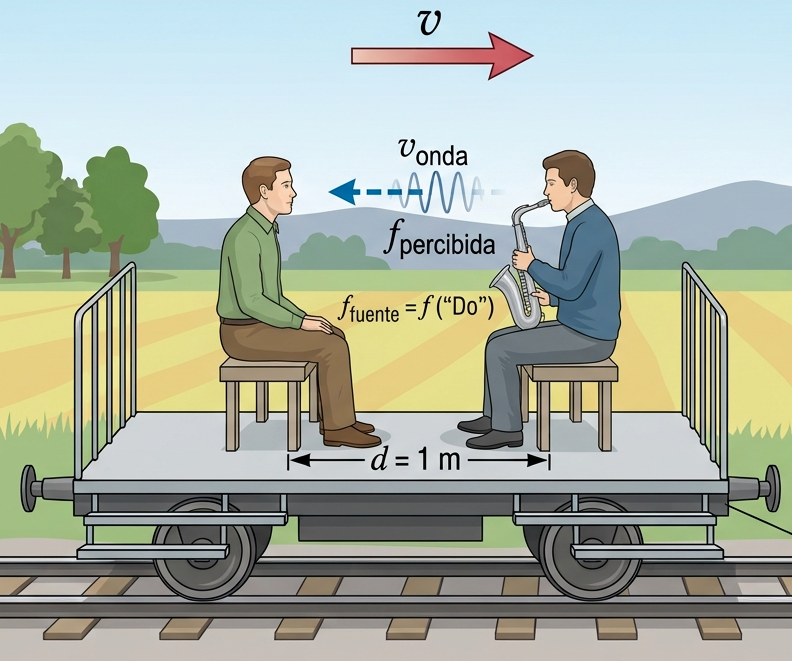
\includegraphics[width=0.45\linewidth]{sound}\hfill
    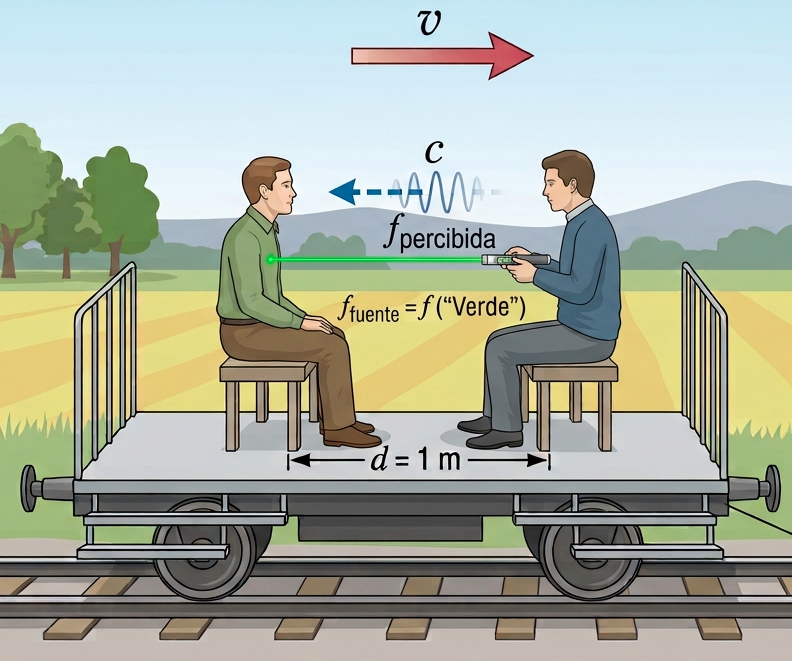
\includegraphics[width=0.45\linewidth]{light}
    \caption{Comparación entre la propagación del sonido y de la luz emitidos desde una
plataforma en movimiento hacia un observador en reposo relativo respecto a la fuente.
    }
    \label{fig:sl}
\end{figure}

Definiendo $c_s\ll c$ como la velocidad del sonido, para la suma de velocidades tenemos en cada caso que 
\begin{align*}
u' =& \frac{u-v}{1-\dfrac{uv}{c^2}}
=\frac{-c_s-v}{1-\dfrac{(-c_s)v}{c^2}}
&
u' =& \frac{u-v}{1-\dfrac{uv}{c^2}}
= \frac{c-v}{1-\dfrac{cv}{c^2}}\\
=&-(c_s+v)\,,
&
=& c\,.
\end{align*}

\begin{tabularx}{\textwidth}{l>{\raggedright\arraybackslash}X>{\raggedright\arraybackslash}X}
\hline
\textbf{} & \textbf{Sonido (``Do'')} & \textbf{Luz (láser verde)} \\
\hline
Velocidad de la onda hacia el observador & $c_s + v$ (depende del medio) & $c$ exactamente (invariante, sin importar $v$) \\
\hline
Frecuencia percibida & $f_0$ (sin Doppler) & $f_0$ (sin Doppler) \\
\hline
Razón de la ausencia de Doppler & Fuente y observador mutuamente en reposo & Fuente y observador mutuamente en reposo \\
\hline
¿Por qué difiere la velocidad de la onda? & El aire define un marco de referencia preferido, distinto al del observador & No existe marco preferido — la luz es $c$ en \textit{todo} marco inercial (postulado de Einstein) \\
\hline
\end{tabularx}


\subsubsection*{Ejemplos Numéricos: Asimetría Clásica vs. Simetría Relativista}

Para ilustrar la diferencia fundamental entre un fenómeno que depende de un medio material (sonido) y uno relativista (luz), analizaremos el caso en el que la velocidad relativa de acercamiento es exactamente la mitad de la velocidad de propagación de la onda.

\paragraph{Caso 1: El Sonido (Física Clásica)}
Supongamos que el aire está en reposo. La velocidad del sonido es $v_s = 340 \text{ m/s}$, la frecuencia emitida es $f_0 = 1000 \text{ Hz}$, y la velocidad de movimiento es $v = 0.5 v_s = 170 \text{ m/s}$.

    
    \textbf{La fuente se aleja del observador (Observador en reposo):} La onda viaja por el aire a la misma velocidad constante de $340 \text{ m/s}$ hacia el observador, pero los frentes de onda se van ``estirando'' físicamente tras el tren. La frecuencia es
    \begin{equation}
        f_{\text{obs}} = f_0 \left( \frac{v_s}{v_s + v} \right) = 1000 \left( \frac{340}{340 + 170} \right) = 666.67 \text{ Hz}.
    \end{equation}


\paragraph{Caso 2: La Luz (Relatividad Especial)}
Para la luz, la velocidad es $c \approx 300,000 \text{ km/s}$, la frecuencia original es $f_0 = 1000 \text{ THz}$, y la velocidad de alejamiento es $v = 0.5 c$.
En relatividad, no hay éter ni medio de referencia. No importa quién se considere ``en reposo'', la luz golpeará a ambos observadores a velocidad $c$. Usamos la versión de alejamiento de la fórmula que derivamos previamente:

\begin{equation}
    f_{\text{obs}} = f_0 \sqrt{\frac{1 - \beta}{1 + \beta}}\,\,.
\end{equation}
donde $\beta=v/c$.
Sustituyendo $v = 0.5 c$:
\begin{equation}
    f_{\text{obs}} = 1000 \sqrt{\frac{1 - 0.5}{1 + 0.5}} = 1000 \sqrt{\frac{0.5}{1.5}} = 1000 \sqrt{\frac{1}{2}}.
\end{equation}
Lo que nos da un resultado simétrico y único:
\begin{equation}
    f_{\text{obs}} \approx 577.35 \text{ THz}.
\end{equation}

\textbf{Conclusión de la Luz:} Gracias a la dilatación del tiempo y a la geometría relativista, las transformaciones de Lorentz garantizan que la velocidad de la onda no cambie (sigue siendo $c$), manifestándose el alejamiento únicamente como un corrimiento al rojo de la  frecuencia de la luz. Del ultravioleta al verde en este caso, pues el verde va de $526$--$\qty{606}{THz}$.




\subsubsection{Ejemplo: Transmisión de Video en un Viaje Interestelar Ultrarrelativista}

    Como aplicación directa de las fórmulas de Efecto Doppler relativista que acabamos de
derivar (Ecuación \eqref{eq:doppler_aleja} y su versión inversa para el acercamiento), analicemos un caso extremo
y muy ilustrativo: una nave que viaja a $\beta = v/c = 0.9999999$ realiza un viaje de ida y
vuelta a un destino situado a $D = 50\,000$ años luz, transmitiendo hacia la Tierra, en tiempo
real  el video grabado a bordo.

    ¿A qué velocidad de reproducción, y con qué duración total, recibiría la Tierra esta
transmisión?

Paso 1: El factor de Lorentz. Con $\beta = 0.9999999$, tenemos
\begin{equation}
    \gamma = \frac{1}{\sqrt{1-\beta^2}} \approx 2236.07.
\end{equation}

Paso 2: El tiempo propio de cada tramo. Cada tramo de $50\,000$ años luz dura, medido
desde la Tierra, aproximadamente $t_{\text{Tierra}} = D/(\beta c) \approx 50\,000$ años. Por
dilatación del tiempo, el tiempo propio $\tau$ que efectivamente transcurre —y que la
tripulación graba— en cada tramo es
\begin{equation}
    \tau_{\text{tramo}} = \frac{t_{\text{Tierra}}}{\gamma} \approx \frac{50\,000}{2236.07}
    \approx 22.36 \text{ años}.
\end{equation}
El metraje total grabado durante el viaje completo (ida y vuelta) es, por lo tanto,
$\tau_{\text{total}} \approx 44.72$ años.

Paso 3: El factor Doppler de alejamiento. Durante el tramo de ida, la nave se aleja, y la
frecuencia de la señal recibida en la Tierra está dada directamente por la Ecuación~\eqref{eq:doppler_aleja}:
\begin{equation}
    f_{\text{obs}} = f_0\sqrt{\frac{1-\beta}{1+\beta}} \quad\Longrightarrow\quad
    \frac{1}{\sqrt{(1-\beta)/(1+\beta)}} = \gamma(1+\beta) \approx 4472.1.
\end{equation}
donde hemos usado la identidad~\eqref{eq:doppid} tal que, de acuerdo a la ec.~\eqref{eq:tobs0}
\begin{equation}
    T\approx 4472 T_0\,.
\end{equation}
Este factor representa cuánto se \textit{estira} cada intervalo de tiempo de la señal: cada
segundo grabado a bordo tarda, en llegar a la Tierra, el equivalente a 4472 segundos (poco
más de 74 minutos).

Paso 4: El factor Doppler de acercamiento. Durante el tramo de vuelta, por la nota que
acompaña a la Ecuación \eqref{eq:doppler_aleja}, simplemente invertimos los signos, obteniendo el recíproco
exacto del factor anterior:
\begin{equation}
    \gamma(1-\beta) \equiv \frac{1}{\gamma(1+\beta)} \approx \frac{1}{4472.1} \approx
    2.236\times10^{-4}.
\end{equation}
Este factor representa cuánto se \textit{comprime} cada intervalo de tiempo de la señal
durante el regreso.

Paso 5: Duración de recepción de cada tramo. Multiplicando el tiempo propio de cada
tramo (Paso 2) por el factor de estiramiento o compresión correspondiente:
\begin{align}
    t_{\text{recepción, ida}} &\approx 22.36 \text{ años} \times 4472.1 \approx 100\,000
    \text{ años},\\
    t_{\text{recepción, vuelta}} &\approx 22.36 \text{ años} \times 2.236\times10^{-4}
    \approx 0.005 \text{ años} \approx 1.8 \text{ días}.
\end{align}

    La Tabla \ref{tab:doppler-nave} resume el resultado.

\begin{table}[h]
\centering
\begin{tabular}{lcc}
\hline
\textbf{Fase} & \textbf{Duración a bordo} & \textbf{Duración de recepción en la Tierra} \\
\hline
Ida (se aleja)   & $\approx 22.36$ años & $\approx 100\,000$ años (cámara ultra lenta) \\
Vuelta (se acerca) & $\approx 22.36$ años & $\approx 1.8$ días (cámara ultra rápida) \\
\hline
\textbf{Total} & $\approx 44.72$ años & $\approx 100\,000$ años \\
\hline
\end{tabular}
\caption{Resultado del Ejemplo 5: transmisión sin compensación de un viaje de ida y vuelta
a $50\,000$ años luz, con $\beta = 0.9999999$.}
\label{tab:doppler-nave}
\end{table}

    Conclusión: A pesar de que la tripulación solo envejece $44.72$ años, la Tierra recibe la
transmisión completa a lo largo de aproximadamente $100\,000$ años —esencialmente la duración
completa del viaje medida desde la Tierra—, ya que prácticamente todo ese tiempo se consume en
recibir, extremadamente estirado, el metraje de la fase de alejamiento. El metraje del regreso,
en cambio, llega comprimido en apenas un par de días, justo antes de que la propia nave aterrice.

\begin{quote}
\textit{Nota:} Este resultado no es un simple artificio matemático: es la manifestación directa
de un límite impuesto por la causalidad. Ninguna técnica de compensación, por avanzada que sea,
podría lograr que la señal de la fase de alejamiento llegue \textbf{más rápido} que el límite
dado por el factor $\gamma(1+\beta)$, ya que esto requeriría transmitir cada fotograma antes de
haber sido grabado. En cambio, sí es físicamente posible \textit{retrasar} deliberadamente la
transmisión durante el acercamiento —comprimiendo aún más, o incluso "estirando" artificialmente
la señal de vuelta si así se desea—, precisamente porque un retraso adicional nunca viola la
causalidad.
\end{quote}

\begin{quote}
\textit{Nota Conceptual — Doppler y la Paradoja de los Gemelos:} Este método, en el que se
analiza exclusivamente la señal luminosa que un observador efectivamente recibe (en vez de
razonar sobre la "simultaneidad a distancia" entre eventos separados), se conoce en la literatura
como el método de Bondi o \textit{k-calculus}. Su virtud es que resuelve la clásica Paradoja de
los Gemelos sin necesidad de invocar la relatividad de la simultaneidad: basta con verificar que
la suma del metraje recibido en ambas fases ($100\,000$ años de estiramiento más $1.8$ días de
compresión) sigue correspondiendo exactamente a los $44.72$ años de metraje real grabado a bordo.
La enorme asimetría entre "ver la fase de ida en cámara lentísima" y "ver la fase de vuelta en
cámara rapidísima" es, precisamente, la forma en que la información —transmitida siempre dentro
de los límites impuestos por $c$— codifica la diferencia de edades entre ambos gemelos.
\end{quote}

\subsubsection{Aplicación Tecnológica: El Telescopio Espacial James Webb y el Espejo de Oro}

Una de las aplicaciones más espectaculares de la física ondulatoria y el efecto Doppler relativista se encuentra en la astronomía observacional moderna, específicamente en el diseño del \textbf{Telescopio Espacial James Webb (JWST)}. Este observatorio está optimizado para mirar hacia el pasado profundo del universo, detectando galaxias formadas apenas unos $300$ millones de años después del Big Bang.

\paragraph{1. El Desafío del Corrimiento al Rojo (\textit{Redshift}):}
A medida que la luz viaja durante más de 13,500 millones de años desde las galaxias más primitivas hasta la Tierra, la expansión del espacio estira físicamente las longitudes de onda de esa radiación. Este fenómeno se cuantifica mediante el corrimiento al rojo ($z$). Para galaxias extremas a un $z = 14$, la luz ultravioleta y visible original llega a nuestro vecindario convertida en radiación \textbf{infrarroja lejana} ($\qty{1.824}{\mu m}$ o superior). Por esta razón, el James Webb opera estrictamente en el infrarrojo. Ver ejercicio~\ref{item:redshift}.

\paragraph{2. El Reto Térmico y los Espejos Recubiertos de Oro:}
Para capturar fotones infrarrojos tan débiles, el telescopio opera en el punto L2 a temperaturas criogénicas (menores a $-233^\circ\text{C}$). Sus 18 segmentos hexagonales están recubiertos con una capa microscópica de \textbf{oro puro}. 

La elección del oro no es estética, sino una consecuencia directa de la \textbf{Relatividad Especial aplicada a la estructura atómica} ($Z = 79$):
\begin{itemize}
    \item \textbf{Naturaleza de la Contracción Interna:} Es importante aclarar que esta contracción interna \textbf{no} es la contracción cinemática de longitudes de Lorentz que experimentan los objetos en movimiento rectilíneo uniforme ($\Delta x = \Delta x_0 / \gamma$). Se trata de un efecto cuántico-relativista derivado de la Ecuación de Dirac: al viajar los electrones más internos ($1s$) a velocidades extremas de aproximadamente el \textbf{$58\%$ de la velocidad de la luz ($0.58c$)}, la solución matemática de su distribución de probabilidad (su función de onda) se comprime espacialmente hacia el núcleo atómico.
    \item \textbf{Ortogonalidad y el Orbital $6s$:} Para que las funciones de onda de los diferentes electrones del átomo no colapsen entre sí, la mecánica cuántica exige una estricta \textbf{ortogonalidad matemática}. Como los orbitales internos $s$ se han contraído profundamente debido a la relatividad, los electrones del orbital externo $6s$ (que se mueven a cerca del \textbf{$35\%$ de la velocidad de la luz, $0.35c$}) se ven obligados por esta condición matemática de ortogonalidad a contraerse también y descender drásticamente en energía para no solaparse con las capas internas.
    \item \textbf{Expansión y Ascenso del Orbital $5d$:} Por su parte, los electrones del orbital $5d$ (que se desplazan a cerca del \textbf{$41\%$ de la velocidad de la luz, $0.41c$}) sufren un efecto de apantallamiento menor debido a la contracción del $6s$, lo que provoca que los orbitales $5d$ se expanda espacialmente y asciendan en energía.
    \item \textbf{Reducción de la Brecha Energética:} Como se ilustra en la Figura \ref{fig:orbitales_oro}, esta reestructuración relativista reduce la diferencia de energía ($\Delta E$) entre los orbitales $5d$ y $6s$. Específicamente, esta brecha se estrecha hasta quedar en el rango de los fotones de luz \textbf{azul y violeta}, cuya energía fotónica se encuentra entre \textbf{$2.75 \text{ eV}$ y $3.10 \text{ eV}$}.
    \item \textbf{Absorción y Reflexión Infrarroja:} Debido a esta menor brecha energética, los electrones del oro absorben con gran eficiencia los fotones de luz azul y violeta (provocando su característico color dorado). Sin embargo, para los fotones de menor energía del \textbf{infrarrojo}, el material carece de mecanismos de absorción a esa escala: la luz infrarroja choca contra el mar de electrones libres de la superficie y es reflejada con una \textbf{reflectividad superior al $98\%$} sin pérdidas térmicas.
\end{itemize}

\begin{figure}[htbp]
\centering
\begin{tikzpicture}[scale=1.2, >=stealth]
    
    % --- ÁTOMO CLÁSICAMENTE ESPERADO (Sin Relatividad) ---
    \begin{scope}[shift={(-2.5,0)}]
        \node[font=\bfseries] at (0, 2.5) {Átomo Hipotético (Clásico)};
        
        % Eje de energía
        \draw[->, thick] (-1, -1.5) -- (-1, 2) node[above] {Energía ($E$)};
        
        % Orbitales 5d y 6s separados por una brecha amplia
        \draw[thick, blue!60!black] (-0.6, 1.2) -- (0.6, 1.2) node[right, font=\footnotesize] {$6s$};
        \draw[thick, red!60!black] (-0.6, -0.8) -- (0.6, -0.8) node[right, font=\footnotesize] {$5d$};
        
        \draw[<->, thick, purple] (0, -0.8) -- (0, 1.2) node[midway, right] {$\Delta E$ grande};
        \node[align=center, font=\scriptsize] at (0, -2.2) {Absorbe en el Ultravioleta\\(Se vería plateado)};
    \end{scope}

    % Flecha de transición
    \draw[->, very thick, orange] (-0.8, 0.5) -- (0.8, 0.5) node[midway, above, font=\scriptsize] {Efectos Relativistas};

    % --- ÁTOMO DE ORO REAL (Con Relatividad) ---
    \begin{scope}[shift={(2.5,0)}]
        \node[font=\bfseries] at (0, 2.5) {Átomo de Oro Real ($Z=79$)};
        
        % Eje de energía
        \draw[->, thick] (-1, -1.5) -- (-1, 2) node[above] {Energía ($E$)};
        
        % Orbitales 5d y 6s acercados por la relatividad
        \draw[thick, blue!60!black] (-0.6, 0.4) -- (0.6, 0.4) node[right, font=\footnotesize] {$6s$ (Contraído/Desciende)};
        \draw[thick, red!60!black] (-0.6, -0.2) -- (0.6, -0.2) node[right, font=\footnotesize] {$5d$ (Expandido/Asciende)};
        
        \draw[<->, thick, purple] (0, -0.2) -- (0, 0.4) node[midway, right] {$\Delta E \approx 2.8 \text{ eV}$};
        \node[align=center, font=\scriptsize] at (0, -2.2) {Absorbe en el Azul ($2.75-3.10\text{ eV}$)\\(Refleja el Infrarrojo)};
    \end{scope}

\end{tikzpicture}
\caption{Diagrama esquemático de los niveles de energía en los orbitales de valencia ($5d$ y $6s$). A la izquierda, un átomo pesado hipotético sin corrección relativista como el aluninio o la plata; a la derecha, el átomo real de Oro ($Z=79$). Los electrones internos a $\approx 0.58c$ contraen el espacio de las funciones de onda; por ortogonalidad matemática, el orbital $6s$ ($\approx 0.35c$) también se contrae y desciende, mientras que el $5d$ ($\approx 0.41c$) asciende. Esto estrecha la brecha energética ($\Delta E$), haciendo que el metal absorba luz azul/violeta y refleje con máxima eficiencia el infrarrojo.}
\label{fig:orbitales_oro}
\end{figure}

% --- Inicio del código LaTeX para insertar ---

\section{Fórmulas del Decaimiento Radiactivo}
En esta sección estableceremos el concepto de vida media para una partícula inestable y veremos cómo la relatividad especial puede afectar el tiempo de vida media dependiendo del observador inercial.

\section*{Introducción: La Naturaleza del Decaimiento}

El decaimiento de una partícula inestable (ya sea un núcleo atómico o una partícula subatómica) es un proceso fundamentalmente \textbf{probabilístico y aleatorio}. No podemos predecir cuándo decaerá una partícula específica. Sin embargo, para una población grande de partículas idénticas, podemos predecir con gran precisión cuántas de ellas decaerán en un intervalo de tiempo determinado.

El principio clave es que la tasa de decaimiento (el número de partículas que decaen por segundo) es directamente proporcional al número de partículas que aún no han decaído. Esto conduce a una ley de \textbf{decaimiento exponencial}.

\section*{Fórmula 1: En Términos de la Constante de Decaimiento ($\lambda$)}

Esta es la forma más fundamental de la ecuación, derivada directamente del principio de proporcionalidad. La tasa de cambio del número de partículas, $N$, con respecto al tiempo, $t$, es:
\[ \frac{dN}{dt} = -\lambda N \]
Donde $\lambda$ (lambda) es la \textbf{constante de decaimiento} y representa la probabilidad de que una sola partícula decaiga por unidad de tiempo. Resolviendo esta ecuación diferencial, obtenemos la \textbf{fórmula del decaimiento exponencial}:
\[ \boxed{N(t) = N_0 e^{-\lambda t}} \]
Donde:
\begin{itemize}
    \item $N(t)$ es el número de partículas que quedan en el tiempo $t$.
    \item $N_0$ es el número inicial de partículas en el tiempo $t=0$.
    \item $e$ es la base del logaritmo natural.
    \item $\lambda$ es la constante de decaimiento, con unidades de (tiempo)\textsuperscript{-1} (p. ej., \si{\per\second}).
\end{itemize}

\section*{Fórmula 2: En Términos de la Vida Media ($t_{1/2}$)}

Esta forma es más intuitiva. La \textbf{vida media ($t_{1/2}$)} es el tiempo que tarda en decaer la mitad de una muestra inicial de partículas.

\subsection*{Relación entre $\lambda$ y $t_{1/2}$}
Podemos encontrar esta relación usando la primera fórmula. Por definición, cuando $t = t_{1/2}$, el número de partículas restantes es $N(t_{1/2}) = N_0/2$.
\[ \frac{N_0}{2} = N_0 e^{-\lambda t_{1/2}} \implies \frac{1}{2} = e^{-\lambda t_{1/2}} \]
Tomando el logaritmo natural de ambos lados:
\[ \ln\left(\frac{1}{2}\right) = -\lambda t_{1/2} \implies -\ln(2) = -\lambda t_{1/2} \]
Esto nos da la relación fundamental:
\[ \boxed{\lambda = \frac{\ln(2)}{t_{1/2}}} \]
Sustituyendo esta expresión para $\lambda$ en la primera fórmula de decaimiento:
\[ N(t) = N_0 e^{-\left(\frac{\ln(2)}{t_{1/2}}\right)t} = N_0 \left(e^{\ln(2)}\right)^{-\frac{t}{t_{1/2}}} = N_0 (2)^{-\frac{t}{t_{1/2}}} \]
Esto nos da la \textbf{fórmula del decaimiento en términos de la vida media}:
\[ \boxed{N(t) = N_0 \left(\frac{1}{2}\right)^{\frac{t}{t_{1/2}}}} \]
Esta forma es muy fácil de interpretar: el exponente ${t}/{t_{1/2}}$ simplemente cuenta ``cuántas vidas medias han pasado'', ver figura~\ref{fig:decrad}.

\begin{figure}[htbp]
\centering
\begin{tikzpicture}[scale=1.1, >=Stealth]

    % Ejes coordenados (ajustados para que y llegue al menos a 110, mapeado a y=5.5)
    \draw[->, thick] (0, 0) -- (6.5, 0) node[right] {};
    \draw[->, thick] (0, 0) -- (0, 5.7) node[above] {};

    % Rótulo del eje horizontal centrado debajo
    \node[align=center] at (3.25, -0.8) {Número de vidas medias};

    % Rótulo del eje vertical rotado 90 grados y centrado a la izquierda
    \node[rotate=90, align=center] at (-1.2, 2.75) {Porcentaje restante};

    % Líneas punteadas de referencia
    % 100% en t=0 (marcas de los ejes)
    %\draw[dashed, gray, thick] (0, 5) -- (5.5, 5);
    
    % 50% en t=1
    \draw[dashed, gray, thick] (1, 0) -- (1, 2.5);
    \draw[dashed, gray, thick] (0, 2.5) -- (1, 2.5);
    
    % 25% en t=2
    \draw[dashed, gray, thick] (2, 0) -- (2, 1.25);
    \draw[dashed, gray, thick] (0, 1.25) -- (2, 1.25);
    
    % 12.5% en t=3
    \draw[dashed, gray, thick] (3, 0) -- (3, 0.625);
    \draw[dashed, gray, thick] (0, 0.625) -- (3, 0.625);

    % Curva de decaimiento exponencial (Función: 5 * e^{-0.693 * x})
    % Mapeo: y=5 corresponde al 100%, y=5.5 corresponderá a 110%
    \draw[red, thick, domain=0:5.8, samples=100] plot (\x, {5 * exp(-0.693147 * \x)});

    % Puntos destacados en la curva
    \fill[red] (1, 2.5) circle (2pt);
    \fill[red] (2, 1.25) circle (2pt);
    \fill[red] (3, 0.625) circle (2pt);

    % Etiquetas en el eje Y (Porcentajes, escala y=5 equivale a 100)
    %\node[left] at (0, 5.5) {$110$};
    \node[left] at (0, 5) {$100$};
    \node[left] at (0, 2.5) {$50$};
    \node[left] at (0, 1.25) {$25$};
    \node[left] at (0, 0.625) {$12.5$};
    
    \draw (0.1, 5) -- (-0.1, 5);
    \draw (0.1, 5.5) -- (-0.1, 5.5);

    % Etiquetas en el eje X (Número de vidas medias)
    \node[below] at (0, 0) {$0$};
    \node[below] at (1, 0) {$1$};
    \node[below] at (2, 0) {$2$};
    \node[below] at (3, 0) {$3$};

    % Textos explicativos superiores
    \node[font=\bfseries] at (3.2, 4.3) {Curva de decaimiento};
    
    \node at (3.5, 3.5) {$\displaystyle N_t = N_0 e^{-\lambda t}$};
    
    \node[align=center, font=\small] at (4.2, 2.6) {
        donde $N_0 = \text{cantidad original}$\\
        $N_t = \text{cantidad final}$
    };

\end{tikzpicture}
\caption{Curva de decaimiento radiactivo en función del número de vidas medias transcurridas.}
\label{fig:decrad}
\end{figure}

\section*{Ejemplos Aplicados}
Aquí aplicamos las fórmulas a tres ejemplos que abarcan escalas de tiempo drásticamente diferentes.

\begin{table}[h!]
\centering
\caption{Comparación de Vidas Medias y Constantes de Decaimiento.}
\label{tab:decay_examples}
\begin{tabular}{l | l | p{2.7cm} | p{5.5cm}}
\hline
\textbf{Partícula} & \textbf{Vida Media ($t_{1/2}$)} & \textbf{C. de Decaimiento ($\lambda$)} & \textbf{Contexto Físico} \\
\hline \hline
Uranio-238 & \SI{4.47e9}{years} & \SI{4.91e-18}{\per\second} & Isótopo extremadamente estable, clave para la datación radiométrica de rocas muy antiguas y la edad de la Tierra. \\
\hline
Neutrón (libre) & \SI{877}{\second} (\SI{14.6}{min}) & \SI{7.9e-4}{\per\second} & Estable dentro de un núcleo, pero inestable cuando está libre. Su vida media es crucial en la cosmología del universo temprano. \\
\hline
Muón & \SI{2.2}{\micro\second} (\SI{2.2e-6}{\second}) & \SI{3.15e5}{\per\second} & Partícula fundamental muy inestable. Su detección en la superficie terrestre es una prueba experimental clásica de la dilatación del tiempo. \\
\hline
\end{tabular}
\end{table}

\paragraph{Cálculos de $\lambda$:}
\begin{itemize}
    \item \textbf{Uranio-238:}
    \begin{itemize}
        \item $t_{1/2} = \SI{4.47e9}{años} \times \SI{3.15e7}{\second\per\text{año}} \approx \SI{1.41e17}{\second}$
        \item $\lambda = \frac{\ln(2)}{\SI{1.41e17}{\second}} \approx \SI{4.91e-18}{\per\second}$
    \end{itemize}
    \item \textbf{Neutrón:}
    \[ \lambda = \frac{\ln(2)}{\SI{877}{\second}} \approx \SI{7.9e-4}{\per\second} \]
    \item \textbf{Muón:}
    \[ \lambda = \frac{\ln(2)}{\SI{2.2e-6}{\second}} \approx \SI{3.15e5}{\per\second} \]
\end{itemize}

% --- Fin del código LaTeX ---



\section{Ejemplos}
\begin{enumerate}
\item Supongamos que un cañón de bolas de tenis es capaz de lanzar una bola de tenis, de diámetro $d = \qty{67}{\milli\m}$  a una velocidad de $0.87c$ hacia la raqueta de un tenista al otro lado de una cancha de longitud $h=\qty{24}{\m}$. Una hormiga accidentalmente resultó viajando con la bola. Calcular el tiempo propio que siente la hormiga y el tiempo dilatado para el tenista. Calcular las distancias contraídas con respecto a cada observador (ver figura \ref{fig:dilcon}). 

\begin{figure}
    \centering
    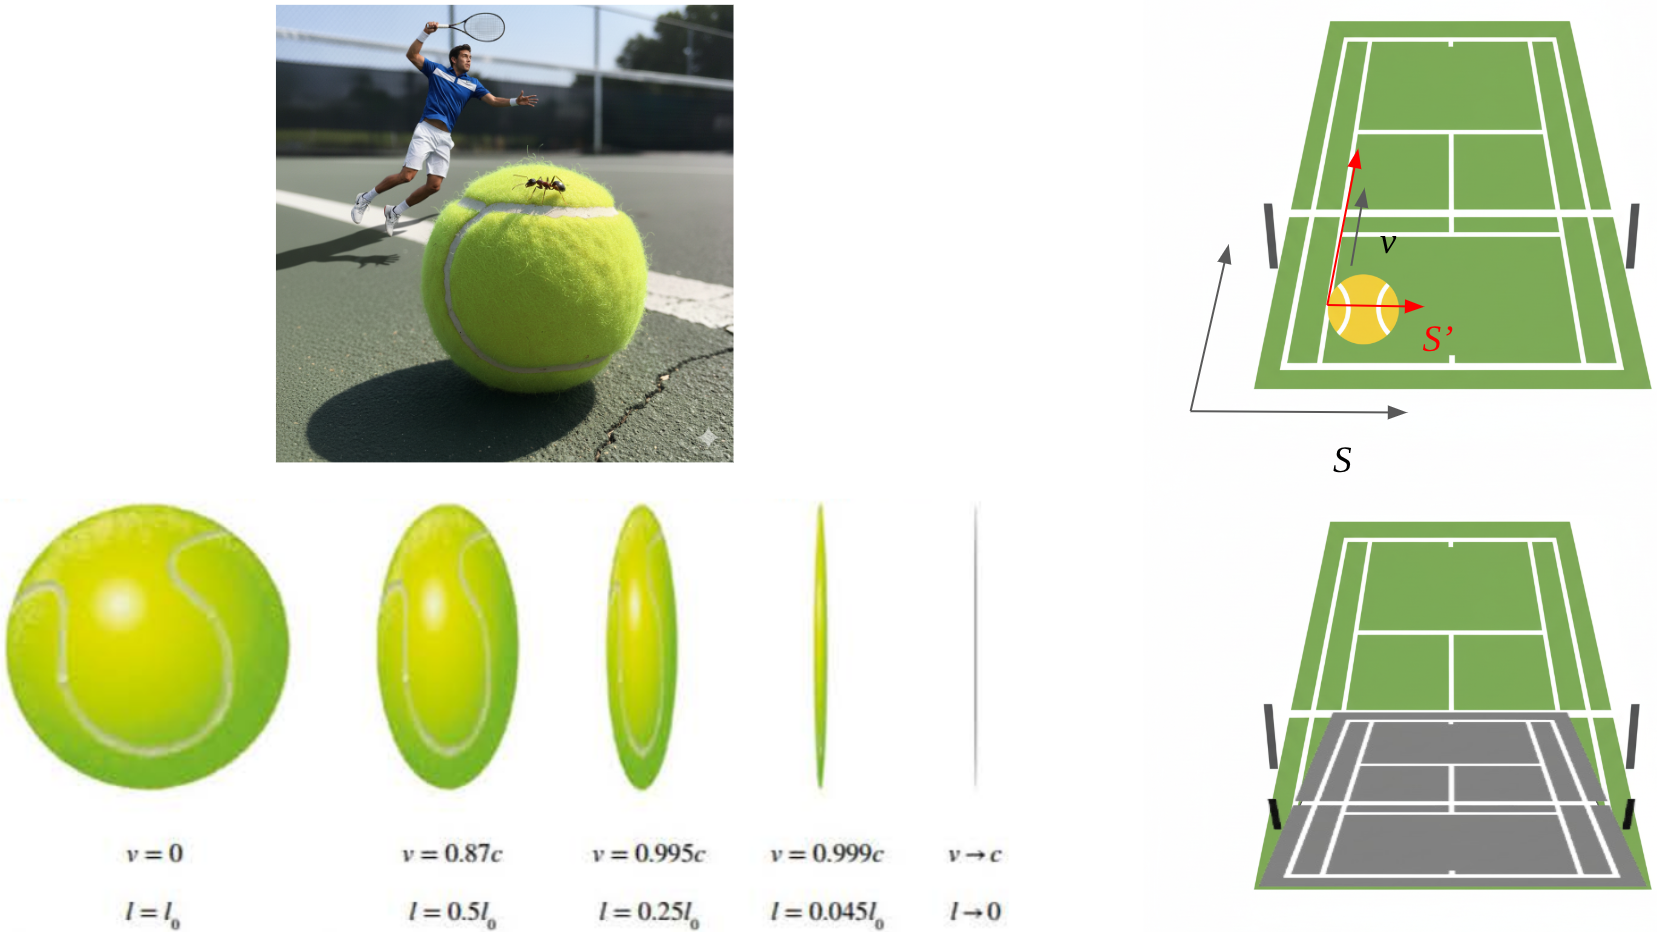
\includegraphics[width=1\linewidth]{tennis.png}
    \caption{Dilatación y contracción en un ejemplo ficticio para una bola de tenis a velocidades relativistas. En la parte  inferior se ilustra de contracción de las longitudes para la bola observada por el tenista, y la contracción de la cancha, en gris, percibida por la hormiga moviendose con la bola de tenis a una velocidad de $0.87c$ correspondiente a una contracción de Lorentz por un factor de $0.5$.}
    \label{fig:dilcon}
\end{figure}

\section*{Solución}
Tenemos que
\begin{itemize}
\item Escogemos el sistema $S$ con origen en el tenista
\item  Escogemos el sistema $S'$ viajando con la bola de tenis.
\item $v = 0.87c$ es la velocidad de la bola con respecto a $S$.
\item Longitud de la cancha de tenis: $h = \qty{24}{m}$ 
\item Diámetro pelota de tenis:  $d = \qty{67}{\milli\m}$
\end{itemize}

El tiempo que tarda la pelota en atravesar la cancha con respecto al tenista es el tiempo dilatado
\begin{align}
    \Delta t = \frac{h}{v} = \frac{\qty{24}{\m}}{0.87\cdot \qty{3e8}{\m/\s}} = \qty{9.2e-8}{\s}\,.
\end{align}

El tiempo que percibe la hormiga es el tiempo propio
\begin{align}
    \Delta t_0 = \frac{\Delta t}{\gamma} =& \Delta t \sqrt{1-v^2/c^2} \nonumber\\
    =& \qty{9.2e-8}{\s} \sqrt{1-0.87^2} \nonumber\\
 \approx &0.5\cdot \qty{9.2e-8}{\s} \nonumber\\
    =& \qty{4.6e-8}{\s}
\end{align}

Para calcular las distancias con respecto al tenista, partimos del hecho que su distancia propia:
\begin{quote}
    La distancia entre dos puntos cuyas posiciones son medidas por
un observador en reposo respecto a los dos puntos,
\end{quote}
corresponde a 
\begin{align*}
    L_0^{c} = h = \qty{24}{m}\,.
\end{align*}
El tenista observa la bola de diámetro propio percibido por la hormiga $L^b_0 = d$, con un diámetro contraído, como se muestra en la parte inferior de la figura~\ref{fig:dilcon}
\begin{align*}
    L^b = \frac{L^b_0}{\gamma} =& d \sqrt{1-v^2/c^2} \\
        =& d\sqrt{1-0.87^2}\\
        \approx& 0.5d\\
    =& 0.5\cdot \qty{67}{\milli\m}\\
    =& \qty{33.5}{\milli\m}\,.
\end{align*}

Finalmente, para las distancias percibidas por la hormiga, partimos del hecho para ella la bola está en su distancia propia $L^b_0 = d$.

Sin embargo, percibe una distancia de la cancha de tenis contraída, dada por
\begin{align*}
    L^{b} = \frac{L^b_0}{\gamma} =& h\sqrt{1-v^2/c^2}\\
    \approx& 0.5 h\\
        =& 0.5\cdot \qty{24}{\m}\\
    =& \qty{12}{\m}\,.
\end{align*}

Podemos de hecho comprobar que en su tiempo propio, $\Delta t_0 = \qty{4.6e-8}{s}$, que es más corto que el tiempo dilatado $\Delta t$, puede recorrer esa distancia contraída con $v=0.87c$
\begin{align*}
    L^{b} = &v \Delta t_0 \\
    =&0.87 c \cdot \qty{4.6e-8}{s}\\
    =&\qty{12}{ m }.
\end{align*}

    
 \item La estrella Xquar está a una distancia de 5 años luz de la
Tierra. La aventurera espacial Raqu se dirige desde la Tierra
hacia Xquar a una velocidad de $0.9c$.
\begin{enumerate}[label=(\alph*)]
    \item Para aquellos que observan desde la Tierra, ¿cuánto tiempo tardará
Raqu en llegar a Xquar?
\item Desde el punto de vista de Raqu, ¿cuánto tiempo tardará ella
en llegar a Xquar?
\item Aunque Xquar estaba a 5 años luz de la Tierra
y Raqu viajó a 0.9c, su viaje tomó mucho
menos tiempo de lo que se podría esperar de estas cifras.
Explique por qué es esto.
\end{enumerate}


\item Un muón es creado en la atmósfera a 15~Km de altura. Viaja hacia el centro de la Tierra a una velocidad de $0.999c$. 
\label{item:muon}

\begin{enumerate}[label=(\alph*)]
    \item Para aquellos que observan desde la Tierra, ¿cuánto tiempo tardará
el muón en llegar a la superficie de la Tierra?
\item Desde el punto de vista del muón, ¿cuánto tiempo tardará
en llegar a la superficie de la Tierra?
\item Aunque la distancia recorrida fue de 15km hasta la superficie de la Tierra y el muón viajó a $0.999c$, 
su viaje tomó mucho
menos tiempo de lo que se podría esperar de estas cifras.
Explique por qué es esto. ¿Es consistente con la vida media del muón?
\end{enumerate}

\section*{Soluciones}

\begin{itemize}
    \item[\ref{item:muon}.]

\textbf{(a) Para aquellos que observan desde la Tierra, ¿cuánto tiempo tardará el muón en llegar a la superficie de la Tierra?}

Esto se pregunta desde la perspectiva del observador ``estacionario'' en la Tierra. El cálculo se basa en la distancia y la velocidad medidas en el sistema de la Tierra.

\begin{itemize}
    \item \textbf{Distancia a recorrer ($L_0$):} 15 km = 15,000 m
    \item \textbf{Velocidad de viaje ($v$):} 0.999c
    \item \textbf{Velocidad de la luz ($c$):} Aproximadamente $3 \times 10^8$ m/s
\end{itemize}
Usamos la fórmula estándar para el tiempo:
\[ \text{Tiempo} = \frac{\text{Distancia}}{\text{Velocidad}} \]
\[ \Delta t = \frac{15,000 \text{ m}}{0.999 \times (3 \times 10^8 \text{ m/s})} = \frac{15,000}{2.997 \times 10^8} \text{ s} \approx 5.005 \times 10^{-5} \text{ s} \]
Para hacer este número más intuitivo, podemos convertirlo a microsegundos ($\mu$s):
\[ 5.005 \times 10^{-5} \text{ s} = 50.05 \times 10^{-6} \text{ s} = 50.05 \, \mu\text{s} \]
\textbf{Respuesta:} Para los observadores en la Tierra, el muón tardará aproximadamente \textbf{50.05 microsegundos} en llegar a la superficie.

\textbf{(b) Desde el punto de vista del muón, ¿cuánto tiempo tardará en llegar a la superficie de la Tierra?}

Esto se pregunta desde la perspectiva del muón en movimiento. El tiempo que el muón experimenta en su propio ``reloj interno'' es el tiempo propio ($\Delta t_0$), que está sujeto a la dilatación del tiempo.

Primero, calculamos el factor de Lorentz ($\gamma$) para una velocidad de 0.999c:
\[ \gamma = \frac{1}{\sqrt{1 - v^2/c^2}} = \frac{1}{\sqrt{1 - (0.999)^2}} = \frac{1}{\sqrt{1 - 0.998001}} = \frac{1}{\sqrt{0.001999}} \]
\[ \gamma \approx 22.37 \]
La fórmula de la dilatación del tiempo es $\Delta t = \gamma \Delta t_0$. Queremos encontrar el tiempo para el muón, $\Delta t_0$:
\[ \Delta t_0 = \frac{\Delta t}{\gamma} = \frac{50.05 \, \mu\text{s}}{22.37} \approx 2.24 \, \mu\text{s} \]
\textbf{Respuesta:} Desde el punto de vista del muón, su viaje a la superficie toma solo \textbf{2.24 microsegundos}.

\textbf{}{(c) Explicación y Consistencia}

Esta pregunta llega al corazón de por qué la relatividad es tan esencial para entender nuestro universo.

\textbf{Explicación de la Diferencia de Tiempo (Contracción de la Longitud)}

La ``paradoja'' se resuelve con la \textbf{contracción de la longitud}. La distancia de 15 km es la \textbf{longitud propia} de la atmósfera medida por alguien en reposo con respecto a ella (en la Tierra).

Desde la perspectiva del muón, está estacionario, y la atmósfera de la Tierra se apresura a su encuentro a 0.999c. Por lo tanto, el muón mide que la altura de la atmósfera está contraída. La distancia contraída ($L$) que ve el muón es:
\[ L = \frac{L_0}{\gamma} = \frac{15 \text{ km}}{22.37} \approx 0.67 \text{ km} \quad (\text{o 670 metros}) \]
Desde el sistema de referencia del muón, su tiempo de viaje tiene perfecto sentido. Se ve a sí mismo cubriendo esta distancia mucho más corta a 0.999c:
\[ \text{Tiempo del Muón} = \frac{\text{Distancia Contraída}}{\text{Velocidad}} = \frac{670 \text{ m}}{0.999 \times (3 \times 10^8 \text{ m/s})} \approx 2.24 \, \mu\text{s} \]
Esto coincide con el resultado de la parte (b). Para el muón, el viaje es corto porque la distancia es corta.

\textbf{}{Consistencia con la Vida Media del Muón}

Esta es la parte más crucial del problema.
\begin{enumerate}
    \item \textbf{Vida Media Propia del Muón:} La vida media de un muón en reposo es aproximadamente $\tau = 2.2 \, \mu\text{s}$.

    \item \textbf{Predicción de la Física Clásica:} Desde el sistema de referencia de la Tierra, el viaje dura $50.05 \, \mu\text{s}$. Como esto es aproximadamente 23 veces más largo que la vida media propia del muón, un físico clásico predeciría que prácticamente ningún muón debería sobrevivir al viaje.

    \item \textbf{Realidad Relativista:}
    \begin{itemize}
        \item \textbf{Desde el Sistema de la Tierra (Dilatación del Tiempo):} El observador en la Tierra ve que el reloj interno del muón funciona lentamente. Su vida media \textit{efectiva} en el sistema de la Tierra está dilatada:
        \[ \text{Vida Media Dilatada} = \gamma \times \tau = 22.37 \times 2.2 \, \mu\text{s} \approx 49.2 \, \mu\text{s} \]
        Como el tiempo de viaje ($50.05 \, \mu\text{s}$) es muy cercano a esta vida media dilatada, es plausible que muchos muones lleguen al suelo.
        \item \textbf{Desde el Sistema del Muón (Contracción de la Longitud):} Desde su propia perspectiva, la vida media del muón es solo su valor normal de $2.2 \, \mu\text{s}$. Sin embargo, el viaje que debe hacer dura solo $2.24 \, \mu\text{s}$ porque la distancia se contrajo. Nuevamente, como el tiempo de viaje y la vida media son casi idénticos, es plausible que el muón sobreviva.
    \end{itemize}
\end{enumerate}
\textbf{Conclusión:} Sí, el viaje es perfectamente consistente con la vida media del muón \textit{cuando se tiene en cuenta la relatividad}. El hecho de que detectemos un gran flujo de muones a nivel del mar es una prueba experimental poderosa tanto de la dilatación del tiempo como de la contracción de la longitud.
\end{itemize}


\item Demuestre que la adición de dos velocidades inferiores a la de luz en la fórmula de adición de velocidades relativistas, no puede superar la velocidad de luz.
\end{enumerate}

% --- REQUIERE EL PAQUETE tcolorbox EN EL PREÁMBULO ---
\begin{tcolorbox}[colback=green!5!white,colframe=green!60!black,title=\textbf{Conexión Interdisciplinaria: Relatividad, Muones y ADN}]

Hemos demostrado matemáticamente que, sin la dilatación del tiempo, los muones cósmicos jamás llegarían a la superficie terrestre. Al viajar a $v \approx 0.999c$, sobreviven el tiempo suficiente para bañar constantemente nuestro planeta. ¿Tiene esto alguna consecuencia para nosotros?

La respuesta une la física relativista con la radiobiología. Los muones son una forma de \textbf{radiación ionizante}. Cada minuto, miles de ellos atraviesan nuestro cuerpo. Aunque interactúan débilmente con la materia (baja transferencia lineal de energía), tienen el potencial físico de arrancar electrones y romper los frágiles enlaces químicos de las cadenas de ADN.

Cuando el ADN se rompe, los mecanismos celulares intentan repararlo. Si cometen un error, se genera una \textbf{mutación genética}. Históricamente, la biología ha considerado que la mayoría de las mutaciones evolutivas provienen de errores internos de la propia célula (procesos endógenos). Sin embargo, investigaciones recientes sugieren que el goteo constante de partículas relativistas actúa como un ruido de fondo que afecta la dinámica celular\footnote{de Groen, P. C. (2022). \textit{Muons, mutations, and planetary shielding}. Frontiers in Astronomy and Space Sciences, 9, 1067491. DOI: \url{https://doi.org/10.3389/fspas.2022.1067491}}.

\textbf{La Prueba Experimental Bajo Tierra:}
Para comprender el impacto real de esta radiación, laboratorios como el \textbf{Gran Sasso} en Italia o el \textbf{SNOLAB} en Canadá cultivan células bajo kilómetros de roca, bloqueando casi el $100\%$ de los muones. Sorprendentemente, en esta ``oscuridad cósmica'', los organismos no prosperan mejor; por el contrario, sus mecanismos de reparación de ADN se atrofian y su respuesta al estrés disminuye. 

Aunque el grado exacto en que los muones impulsan las mutaciones evolutivas a largo plazo sigue siendo objeto de un fascinante debate científico, la evidencia demuestra que la vida en la Tierra evolucionó en sintonía con este bombardeo relativista y depende de él para mantener sus defensas celulares activas.
\end{tcolorbox}


\section{Espacio de Minkowski}

%\section{Unidades Naturales y Rapidez}
Para tener las coordenadas con las mismas unidades,, debemos usar $ct$ para que sea interpretado como una dimensión espacial
\begin{align}
ct' =& \gamma\left(ct-\frac{v}{c}x\right),\\
x'=&\gamma\left(x-\frac{v}{c}ct\right)
\end{align}

\

\subsection{Funciones Hiperbólicas}
\begin{align*}
    \cosh x =& \frac{{e}^{x}+{e}^{-x}}{2}\,,&
\sinh x =& \frac{{e}^{x}-{e}^{-x}}{2}\,.
\end{align*}
Por lo tanto
\begin{align*}
    \cosh^2x - \sinh^2x =& \frac{({e}^{x}+{e}^{-x})^2
    -({e}^{x}-{e}^{-x})^2}{4}\\
    =&\frac{{e}^{2x}+2{e}^{x}{e}^{-x}+{e}^{-2x}
-({e}^{2x}-2{e}^{x}{e}^{-x}+{e}^{-2x})}{4}\\
=&\frac{\cancel{{e}^{2x}}+2+\cancel{{e}^{-2x}}
-\cancel{{e}^{2x}}+2-\cancel{{e}^{-2x}}}{4}\\
=&\frac{4}{4}\\
=&1
\end{align*}

Podemos parametrizar la velocidad usando la \textbf{rapidez}, $\xi$:
\[ \gamma = \cosh\xi, \quad -\frac{v}{c}\gamma = \sinh\xi \]
Esta parametrización es válida porque satisface automáticamente la identidad $\gamma^2(1-v^2)=1$:
\[ \cosh^2\xi - \sinh^2\xi = \gamma^2 - \left(-\frac{v}{c}\gamma\right)^2 = \gamma^2\left(1-\frac{v^2}{c^2}\right) = 1 \]
A partir de esto, también encontramos que la velocidad está relacionada con la rapidez por 
\begin{align*}
    -\frac{v}{c} = \tanh\xi\,,
\end{align*}
donde
\begin{align*}
\tanh\xi \equiv \frac{\sinh\xi}{\cosh\xi}\,.    
\end{align*}

En resumen, las transformaciones de Lorentz se pueden escribir como
\[
\boxed{
\begin{aligned}    
    ct' =& ct\cosh\xi + x\sinh\xi \\
    x' = &x\cosh\xi + ct\sinh\xi\\
    y' = & y\\
    z' = &z\,.
\end{aligned}
}
\]

Si definimos la coordenada temporal en la dimensiones de distancia como $x^0\equiv ct$, podemos definir el cuadrivector de impulso (boost)
\begin{align}
    x^\mu \equiv \left(x^0, x^1, x^2,x^3 \right) = \left(ct, x, y,z \right)
    = (ct,\boldsymbol{r})
\end{align}
donde hemos usado el superíndice $\mu$ para denotar un vector de impulso, enfatizando que pertenece a un espacio diferente con una dimensión temporal y las correspondientes dimensiones espaciales, llamado espacio de Minkowski Minkowski.
El vector de impulso se transforma bajo una transformación de Lorentz como
\[
\boxed{
\begin{aligned}    
    {x^0}' =& x^0\cosh\xi + x^1\sinh\xi \\
    {x^1}' = &x^1\cosh\xi + x^0\sinh\xi\\
    {x^2}' = & x^2\\
    {x^3}' = &x^3\,.
\end{aligned}
}
\]

A continuación trabajaremos en dos dimensiones, una temporal y una espacial, de manera que el vector de impulso es
\begin{align}
\label{eq:bivector}
    x^\mu \equiv \left(x^0, x^1 \right) = \left(ct, x \right)
\end{align}

\subsection{Invariancia bajo transformaciones de Lorentz}
En la ecuación~\eqref{eq:so3} vimos que el producto escalar era invariante bajo rotaciones en el espacio.

Verifiquemos, bajo qué condiciones el módulo del vector de impulso es invariante bajo transformaciones de Lorentz. 
Definimos el producto escalar entre dos vectores de impulso (en el espacio de Minkowski)
$x^\mu = (x^0,x^1)$ y $y^\mu = (y^0,y^1) $ como
\begin{align}
    x^\mu \cdot y^\mu = g_{00} x^0 y^0 + g_{11} x^1 y^1\,.
\end{align}
con $g_{00}$ y $g_{11}$ a ser fijados por la condición de invarianza. 

El vector de impulso en la base transformada es, 
\begin{align*}
{x'}^\mu = ({x'}^0,{x'}^1) = ({x^0}\cosh\xi + {x^1}\sinh\xi, {x^1}\cosh\xi +{x^0}\sinh\xi),
\end{align*}
El producto escalar en el espacio de Minkowski del vector de impulso consigo mismo es 
\begin{align*}
    {x'}^\mu \cdot {x'}^\mu =& 
g_{00} \left({x^0}'\right)^2 + g_{11} \left({x^1}'\right)^2 \\
=& g_{00}\left[\left({x^0}\right)^2\cosh^2\xi -2 {x^0}{x^1}\cosh\xi\sinh\xi+\left({x^1}\right)^2\sinh^2\xi\right]\\
&+
g_{11}\left[\left({x^1}\right)^2\cosh^2-2{x^0}{x^1}\cosh\xi\sinh\xi + \left({x^0}\right)^2\sinh^2\xi\right].
\end{align*}
Si $g_{00}=1$ y $g_{11}=-1$, el producto escalar en el espacio de Minkowski resulta ser invariante, ya que, usando $\cosh^2\xi-\sinh^2\xi=1$
\begin{align*}
        {x'}^\mu \cdot {x'}^\mu   
=& \left({x^0}\right)^2(\cosh^2\xi-\sinh^2\xi)+\left({x^1}\right)^2(\sinh^2\xi-\cosh^2\xi) -\cancel{2 {x^0}{x^1}\cosh\xi\sinh\xi}+\cancel{2 {x^0}{x^1}\cosh\xi\sinh\xi}\\
=&\left({x^0}\right)^2 - \left({x^1}\right)^2\\
=&x^\mu\cdot x^\mu\,.
\end{align*}
donde $x^\mu$ esta definido en la ecuación~\eqref{eq:bivector}.




Generalizando a todas las coordenadas del espacio-tiempo, tenemos que el producto escalar entre $x^\mu=(x^0,x^1, x^2, x^3$ y $y^\mu=(y^0,y^1,y^2,y^3)$ en el espacio de Minkowski es
\begin{align}
    x^\mu\cdot y^\mu =& x^0 y^0 -x^1 y^1 -x^2 y^2 -x^3 y^3\,.
\end{align}

\begin{figure}
    \centering
\begin{tikzpicture}[>=stealth, scale=0.8]
    
    % Vectores
    \draw[->, thick, blue] (0,0) -- (4,2) node[midway, below right] {$x_1^\mu$};
    \draw[->, thick, red] (0,0) -- (1,3) node[midway, left] {$x_2^\mu$};    
    % Vector diferencia
    \draw[->, thick, green!60!black] (1,3) -- (4,2) node[midway, above right] {$x^\mu_2 - x^\mu_1$};
\end{tikzpicture}
    \caption{$\Delta x^\mu = x^\mu_2 - x^\mu_1$}
    \label{fig:b2-b1}
\end{figure}

Similarmente, para la diferencia de dos impulsos, como en la figura~\ref{fig:b2-b1}
\begin{align*}
    \Delta x^\mu = x^\mu_2 - x^\mu_1 
\end{align*}
tiene un módulo al cuadrado, que es invariante
\begin{align*}
    \Delta S^2 =& \Delta x^\mu\cdot \Delta x^\mu \\ 
     =&\left(x^0_2-x^0_1\right)^2 -\left(x_2-x_1\right)^2
    -\left(y_2-y_1\right)^2-\left(z_2-z_1\right)^2\\
    =&\left(ct_2- c t_1\right)^2 -\left(x_2-x_1\right)^2
    -\left(y_2-y_1\right)^2-\left(z_2-z_1\right)^2\,,
\end{align*}
%
tenemos así el \emph{intervalo invariante}
\begin{align*}
    \Delta S^2 =
     &c^2\Delta t^2 - \Delta x^2 - \Delta y^2 - \Delta z^2\,. 
\end{align*}


% ---------------------------------------------------------
% 1. Definición segura de los iconos (Pega esto en el preámbulo)
% SIN NINGUNA LÍNEA EN BLANCO DENTRO DE LOS COMANDOS
% ---------------------------------------------------------

\newcommand{\iconoRegla}{%
\begin{tikzpicture}[baseline=-0.5ex, scale=0.25]
\draw[thick, fill=yellow!20] (0,-0.5) rectangle (4,0.5);
\foreach \x in {0.5, 1.5, 2.5, 3.5} \draw[thick] (\x, 0.5) -- (\x, 0.2);
\foreach \x in {1, 2, 3} \draw[thick] (\x, 0.5) -- (\x, 0);
\end{tikzpicture}%
}

A pesar que los relojes y reglas se transforman al cambiar de sistema de referencia inercial, el intervalo invariante es absoluto (independiente del sistema de referencia inercial). Gráficamente
%
\begin{equation}
\Delta S^2 =c^2\cdot {
\includegraphics[scale=0.03]{clock}}^2 -  \iconoRegla^{\,2}\,.
\end{equation}

%\begin{equation}
%    x^\mu = \Bigg( c \cdot \iconoReloj \; , \;\; \iconoRegla \Bigg).
%\end{equation}



\section{Derivación de la Energía y el Momento Relativista a partir del Cuadrivector}

En la mecánica clásica, el momento se define como la masa multiplicada por la velocidad ($\boldsymbol{p} = m\boldsymbol{v}$). Sin embargo, en relatividad, la velocidad espacial $\boldsymbol{v} = \Delta \boldsymbol{r} / \Delta t$ presenta un problema fundamental: aunque la distancia $\Delta \boldsymbol{r}$ y el tiempo $\Delta t$ se transforman al cambiar de sistema de referencia, no lo hacen de una manera que garantice que las leyes de conservación se mantengan para todos los observadores.

Para formular una ley de conservación del momento que sea válida universalmente, debemos construir un vector en el espacio de Minkowski (un \textbf{cuadrivector}) cuyo producto escalar consigo mismo sea un \textbf{invariante relativista}.

\subsubsection{Paso 1: El Tiempo Propio como Invariante}

Recordemos que el producto escalar del cuadrivector de desplazamiento $\Delta X^\mu = (c\Delta t, \Delta \boldsymbol{r})$ consigo mismo nos da el intervalo invariante $\Delta s^2$:
\begin{equation}
    \Delta S^2 = (c\Delta t)^2 - |\Delta \boldsymbol{r}|^2.
\end{equation}
Para un observador que viaja junto con la partícula, la partícula no se mueve ($\Delta \boldsymbol{r} = 0$), y el tiempo que mide su reloj es el \textbf{tiempo propio} ($\Delta \tau$). Para este observador, el intervalo es simplemente
\begin{equation}
    \Delta S^2 = (c\Delta t_0)^2.
\end{equation}
Como $\Delta s^2$ es un invariante (todos los observadores miden el mismo valor), podemos igualar ambas expresiones:
\begin{equation}
    c^2 \Delta t_0^2 = c^2 \Delta t^2 - |\Delta \boldsymbol{r}|^2.
\end{equation}
Dividiendo toda la ecuación por $c^2 \Delta t^2$, obtenemos
\begin{equation}
    \left( \frac{\Delta t_0}{\Delta t} \right)^2 = 1 - \frac{|\Delta \boldsymbol{r}|^2}{c^2 \Delta t^2} = 1 - \frac{v^2}{c^2}.
\end{equation}
Reconociendo el inverso del factor de Lorentz ($1/\gamma^2$), llegamos a la profunda relación entre el tiempo del laboratorio y el tiempo propio
\begin{equation}
    \Delta t = \gamma \Delta t_0.
    \label{eq:tiempo_propio}
\end{equation}
El tiempo propio $\Delta t_0$ es una magnitud escalar invariante, acordada por todos los observadores.

\subsubsection{Paso 2: Construcción de la Cuadrivelocidad}

Para crear un vector de velocidad que se comporte correctamente bajo las transformaciones de Lorentz, debemos tomar el cuadrivector de posición $\Delta X^\mu$ y dividirlo, no por el tiempo relativo $\Delta t$, sino por el tiempo invariante $\Delta t_0$. Definimos así la \textbf{cuadrivelocidad} $V^\mu$:
\begin{equation}
    V^\mu = \frac{\Delta x^\mu}{\Delta t_0} = \left( c\frac{\Delta t}{\Delta t_0}, \frac{\Delta \boldsymbol{r}}{\Delta t_0} \right).
\end{equation}
Utilizando la regla de la cadena 
$$\frac{\Delta \boldsymbol{r}}{\Delta t_0} = \frac{\Delta \boldsymbol{r}}{\Delta t} \frac{\Delta t}{\Delta t_0}$$
y la ecuación (\ref{eq:tiempo_propio}), podemos expresar $V^\mu$ en términos de las variables medidas en el laboratorio ($v$ y $\gamma$):
\begin{align}
    V^\mu =& \left(c\frac{\Delta t}{\Delta t/\gamma},
    \frac{\Delta \boldsymbol{r}}{\Delta t/\gamma}
    \right)\nonumber\\
    =& \left(\gamma c,
    \gamma\frac{\Delta \boldsymbol{r}}{\Delta t}
    \right)\nonumber\\
    V^\mu =& ( \gamma c, \gamma \boldsymbol{v} ),
\end{align}
donde hemos usado que
\begin{align*}
\boldsymbol{v} = \frac{\Delta \boldsymbol{r}}{\Delta t}\,.
\end{align*}
Comprobemos que su producto escalar es efectivamente un invariante que no puede depender de la velocidad del sistema de referncia inercial, $v$:
\begin{equation}
    V^\mu \cdot V^\mu = (\gamma c)^2 - (\gamma v)^2 = \gamma^2 (c^2 - v^2) = \left( \frac{1}{1 - v^2/c^2} \right) c^2 \left( 1 - \frac{v^2}{c^2} \right) = c^2.
\end{equation}
El resultado es $c^2$, una constante universal. ¡Nuestra construcción geométrica funciona a la perfección!

\subsubsection{Paso 3: El Cuadrimomento y las Nuevas Definiciones}

Ahora, multiplicamos la cuadrivelocidad por la masa en reposo de la partícula, $m$. Dado que $m$ es otro escalar invariante (no depende de la velocidad del sistema de referencia inercial, $v$), el resultado será un nuevo cuadrivector garantizado, llamado \textbf{cuadrimomento} ($P^\mu$):
\begin{equation}
    p^\mu = m V^\mu = ( \gamma m c, \gamma m \boldsymbol{v} ).
\end{equation}
Identificamos las componentes de este nuevo vector con las cantidades dinámicas físicas:

\textbf{1. El Momento Relativista:}
La parte espacial de nuestro cuadrivector corresponde a la generalización natural del momento lineal clásico. Por lo tanto, definimos rigurosamente el momento relativista como
\begin{equation}
    \boldsymbol{p} = \gamma m \boldsymbol{v}.
    \label{eq:momento_relativista}
\end{equation}

\textbf{2. La Energía Total Relativista:}
Consideremos ahora la componente temporal del
cuadrimomento, $\gamma mc$. Un análisis dimensional revela que (como era de esperarse) esta cantidad tiene
unidades de momento lineal ($\text{M}\cdot\text{L}/\text{T}$, las mismas que $mv$). Para construir una cantidad con dimensiones de energía
($\text{M}\cdot\text{L}^2/\text{T}^2$), multiplicamos por la única velocidad
invariante disponible en la teoría, $c$:
\begin{equation}
    E \equiv \gamma mc^2 .
\end{equation}
Esta es, por ahora, solo una \emph{candidata} razonable a la energía total relativista
--- una hipótesis motivada por el análisis dimensional, no todavía una conclusión
demostrada. Para justificarla físicamente, invocamos el \textbf{Principio de
Correspondencia}: toda teoría física nueva debe reducirse a la teoría antigua,
ya verificada experimentalmente, en el régimen donde esta última es válida. En
nuestro caso, la mecánica newtoniana debe emerger de la Relatividad Especial en
el límite de bajas velocidades ($v \ll c$).

Verifiquemos si nuestra candidata pasa esta prueba. Usando la aproximación
binomial para $v \ll c$,
\begin{equation}
    (1+x)^n \approx 1 + nx, \qquad \text{si } x \ll 1,
\end{equation}
con $x = -v^2/c^2$ y $n = -1/2$, obtenemos
\begin{align*}
\gamma =& \frac{1}{\sqrt{1-\frac{v^2}{c^2}}}&&\\
=& \left(1-\frac{v^2}{c^2}\right)^{-1/2}&&\\
\approx& 1 + \frac{1}{2}\frac{v^2}{c^2}\,,&\text{sí\quad } \frac{v^2}{c^2}\ll 1\,.
\end{align*}
Entonces
\begin{equation}
\label{eq:Ereposomascinetica}
    E \approx m c^2 \left( 1 + \frac{1}{2}\frac{v^2}{c^2} \right) = m c^2 + \frac{1}{2} m v^2\,.
\end{equation}
El resultado es exactamente lo que el Principio de Correspondencia exige: el segundo
término es la energía cinética clásica de Newton, ya conocida y verificada
experimentalmente durante siglos. El primer término, $mc^2$, es un término
completamente nuevo --- una energía intrínseca que la partícula posee incluso en
reposo ($v=0$), sin análogo en la mecánica newtoniana.

Como nuestra candidata $E=\gamma mc^2$ se reduce correctamente a toda la física
clásica conocida en el límite apropiado, aceptamos que efectivamente representa la
energía total relativista de la partícula:
\begin{equation}
    E = \gamma mc^2 .
\end{equation}



\subsubsection{Conclusión: El Invariante Energía-Momento}

Al sustituir nuestras nuevas definiciones (\ref{eq:momento_relativista}) y (\ref{eq:energia_relativista}) de vuelta en el cuadrimomento, obtenemos 
\begin{align}
p^\mu = (E/c, \boldsymbol{p}).     
\end{align}
Evaluando nuevamente su producto escalar invariante, tenemos
\begin{align}
\label{eq:cuadrimomentumsquare}
    p^\mu \cdot p^\mu =&\left( \frac{E}{c} \right)^2 - |\boldsymbol{p}|^2\nonumber\\
    p^\mu \cdot p^\mu =&\left( \frac{E}{c} \right)^2 - p^2\\
    =& \gamma^2m^2\left(c^2-v^2\right)\nonumber\\
    =& \gamma^2m^2 c^2\left(\frac{c^2-v^2}{c^2}\right)\nonumber\,,
\end{align}
usando la ec.~\eqref{eq:gammasquare} para $\gamma^2$
\begin{align}
p^\mu \cdot p^\mu =&\cancel{\gamma^2} m^2 c^2\frac{1}{\cancel{\gamma^2}}\nonumber\\
    =& m^2 c^2\,,    
\end{align}
que como era de esperarse no puede depender de la velocidad del sistema de referencia inercial $v$

Multiplicando por $c^2$ y reorganizando la ec.~\eqref{eq:cuadrimomentumsquare}
\begin{align*}
m^2c^2 =& \frac{E^2}{c^2} - p^2 \\
m^2c^4 =& E^2 - p^2 c^2\\
\left(m c^2\right)^2 =& E^2 - \left(p c\right)^2\,,
\end{align*}
llegamos a la joya de la corona de la dinámica relativista, válida para cualquier partícula en el universo:
\begin{equation}
\label{eq:energiarelativista}
    E^2 = (m c^2)^2 + (p c)^2.
\end{equation}

Note que una partícula de masa cero, como el fotón, tiene una energía (definidad positiva) asociada a la cantidad de movimiento que transporta
\begin{equation}
\label{eq:Em=0}
    \lim_{m\to 0} E = pc\,.
\end{equation}

\subsection{Límites de la energía total relativista}
Tenemos
\begin{align}
\label{eq:E=gammamc2}
    \boxed{E = \gamma m c^2\,.}
\end{align}
Usando la ecuación~\eqref{eq:gammasquare} para $\gamma$, tenemos
\begin{align}
    E = \frac{m c^2}{\sqrt{1-v^2/c^2}}
\end{align}

Por lo tanto
    \begin{align}
        \lim_{v\to c} E = \infty\,.
    \end{align}


De modo que se requeriría  una energía infinita para acelerar un objeto material a la velocidad de la luz. 

De otro lado, la única forma de evitar que una partícula de masa 0 tenga energía total cero es cuando $v=c$ pues sólo en ese caso la energía pasa de ser cero a una indeterminación $0/0$. En ese caso la energía de la partícula de masas cero moviéndose a la velocidad de la luz está dada por la ec.~\eqref{eq:Em=0}
\begin{equation}
    E =pc \quad\text{si $m=0$}\,.
\end{equation}


Además, si aceptamos la existencia de una partícula que se pueda mover más rápido que la velocidad de la luz, llamada taquión, el radicando en el denominandor tendría un signo negativo y la energía sería imaginaria, lo que aparentemente no tiene significado físico. Es de anotar que a la fecha no se ha observado ningún taquión en la naturaleza.




Hay dos límites:

\begin{enumerate}
    \item Límite no relativista: $m\gg p$ que resulta en 
    \begin{align*}
        E = m c^2\,,
    \end{align*}
    que la energía mínima que puede tener un objeto de masa $m$ y se denomina su \emph{energía en reposo}.
    \item Límite relativista: $m \ll p$ que resulta en
    \begin{align*}
        E = pc\,.
    \end{align*}

    Éste límite es válido para partículas con o sin masa (cómo el fotón).  En el caso de un fotón, hemos visto que su energía es 
    \begin{align}
    \label{eq:energiafoton}
        E=h\nu\,,
    \end{align}
    y reemplazando en la expresión anterior, tenemos que el momento de un fotón es 
    \begin{align}
        p=\frac{E}{c} =& \frac{h}{c}\nu\,,
    \end{align}
    lo cual es dimensionalmente consistente porque
    \begin{align}
        [p] =&\frac{E\cdot \cancel{T}}{\dfrac{L}{T}}\cdot \frac{1}{\cancel{T}}\nonumber\\
         =& \frac{M \dfrac{L^{\cancel{2}}}{T^{\cancel{2}}}}{\cancel{\dfrac{L}{T}}}\nonumber\\
        = &M \frac{L}{T}\,,
    \end{align}
    como era de esperarse. 

    La longitud de onda de un fotón es
    \begin{align}
        \lambda =\frac{c}{\nu},,
    \end{align}
tal que $[\lambda] = [L]$ y por lo tanto
\begin{align}
    p =\frac{h}{\lambda}\,.
\end{align}
La correspondiente energía de un fotón de longitud de onda $\lambda$
\begin{align}
E = pc =\frac{hc}{\lambda}\,.    
\end{align}

\end{enumerate}


\subsection{Velocidad relativista}
\label{sec:vfromp1d}
A modo de ejemplo, despejemos la magnitud de la velocidad relativista a partir de la magnitud de su cantidad de movimiento:
\begin{enumerate}
    \item Encuentre el cuadrado de la velocidad a la que se mueve una partícula de masa $m$ a partir de su momento

\renewcommand{\phantom}[1]{#1}

\noindent
 \hspace{-1cm}\begin{tabular*}{0.95\textwidth}{l|c|p{9cm}}
   \textbf{Paso} & \textbf{Ecuación}  & \textbf{Justificación} \\\hline
1)     & $p =\dfrac{m v}{\sqrt{1-\dfrac{v^2}{c^2}}}$   & ecuación inicial.\\[20pt]\hline
2) & $p^2  =\dfrac{m^2 v^2}{1-\dfrac{v^2}{c^2}} $& Elevar ambos lados al cuadrado. \\[20pt]\hline
3) & \phantom{$p^2\left(1-\dfrac{v^2}{c^2}\right)  =m^2 v^2 $}& Multiplicar a ambos lados por $\left(1-\dfrac{v^2}{c^2}\right)$ \\[5pt]\hline
4) & $p^2-\dfrac{p^2v^2}{c^2}  =m^2 v^2 $& Expandir $p^2$ a \emph{ambos} términos del paréntesis en el lado izquierdo. \\[5pt]\hline
5) & \phantom{$  \dfrac{p^2v^2}{c^2} + m^2 v^2 = p^2 $}& Sumar $\dfrac{p^2v^2}{c^2}$ a ambos lados de la igualdad y reorganizar la igualdad con los términos con $v^2$ a la izquierda. \\[5pt]\hline
6) & $v^2\left(\dfrac{p^2}{c^2} + m^2\right)= p^2 $& Factorizar $v^2$. \\[5pt]\hline
7) & \phantom{$v^2=\dfrac{p^2}{m^2 + \dfrac{p^2}{c^2}}$} & Dividir por $\left(\dfrac{p^2}{c^2} + m^2\right)$ a ambos lados de la igualdad. \\[20pt]\hline
\end{tabular*}
\item ¿Bajo que condición se recupera el límite no relativista?
\begin{align*}
    v = \frac{p}{m}\,,
\end{align*}
Asumiendo que la dirección de $p$ es la misma que la de $v$, podemos ignorar la solución con signo menos, de modo que
\begin{align*}
    v=&\dfrac{p}{\sqrt{m^2 + \dfrac{p^2}{c^2}}}\\
    =&\dfrac{p/m}{\sqrt{1 + \dfrac{p^2}{m^2c^2}}}\,.
\end{align*}
Es claro que en si hacemos $c\to \infty$
\begin{align*}
    v =& \frac{p}{m}\,.
\end{align*}

\end{enumerate}


\subsection{Generalización a Tres Dimensiones y Conexión con la Energía}

La ecuación escalar que acabamos de derivar para la rapidez,
\begin{equation}
    v^2 = \frac{p^2}{m^2 + \dfrac{p^2}{c^2}},
\end{equation}
puede generalizarse directamente a tres dimensiones. Por definición, el vector de cantidad de movimiento ($\boldsymbol{p}$) y el vector velocidad ($\boldsymbol{v}$) apuntan siempre en la misma dirección. Su relación fundamental es
\begin{equation}
    \boldsymbol{p} = (\gamma m) \boldsymbol{v}.
\end{equation}

Despejando el vector velocidad, vemos que simplemente debemos dividir el vector $\boldsymbol{p}$ por el factor escalar $(\gamma m)$:
\begin{align}    
    \boldsymbol{v} =& \frac{\boldsymbol{p}}{\gamma m}\nonumber\\
    =&\frac{\boldsymbol{p}}{\dfrac{1}{\sqrt{1-v^2/c^2}} m}\nonumber\\
=&\frac{\boldsymbol{p}}{\dfrac{1}{\sqrt{1-\dfrac{p^2}{\left(m^2+p^2/c^2\right)c^2}}} m}\nonumber\\
=&\frac{\boldsymbol{p}}{\dfrac{1}{\sqrt{1-\dfrac{p^2}{\left(m^2c^2+p^2\right)}}} m}\nonumber\\
=&\frac{\boldsymbol{p}}{\dfrac{1}{\sqrt{\dfrac{m^2c^2+p^2-p^2}{m^2c^2+p^2}}} m}\nonumber\\
=&\frac{\boldsymbol{p}}{\sqrt{\dfrac{m^2c^2+p^2}{\cancel{m^2}c^2}}\cancel{m}}\,.
\end{align}
Finalmente
\begin{align}
\label{eq:velocidadrelativista}
\boldsymbol{v}  =&\frac{\boldsymbol{p}}{\sqrt{m^2+p^2/c^2}}
\end{align}


\textbf{Una Revelación Algebraica: La Conexión con la Energía Total}

Podemos llevar esta expresión vectorial a una forma aún más elegante. Si multiplicamos el numerador y el denominador dentro de la raíz cuadrada por $c^2$, obtenemos:
\begin{equation}
    \boldsymbol{v} = \frac{\boldsymbol{p} c}{\sqrt{m^2 c^2 + p^2}}.
\end{equation}
Al multiplicar y dividir toda la fracción por $c$, la expresión se transforma en
\begin{equation}
    \boldsymbol{v} = \frac{\boldsymbol{p} c^2}{\sqrt{m^2 c^4 + p^2 c^2}}.
\end{equation}

Si observamos el denominador, reconoceremos inmediatamente la joya de la dinámica relativista que derivamos en la Ecuación~\eqref{eq:energiarelativista}: la energía total de la partícula es $E = \sqrt{(mc^2)^2 + (pc)^2}$. 

Al sustituir el denominador por $E$, llegamos a una de las relaciones más compactas, hermosas y útiles de toda la Relatividad Especial:
\begin{equation}
    \boldsymbol{v} = \frac{\boldsymbol{p} c^2}{E}.
\end{equation}

En el \emph{límite no relativista} de $\gamma \approx 1$ en la ec.~\eqref{eq:E=gammamc2}, la energía se reduce a la energía en reposo
\begin{equation}
    E=\gamma m c^2\approx mc^2\,,
\end{equation}
de modo que 
\begin{align}
\label{eq:nonrelativistcvelocity}
    \boldsymbol{v} \approx & \frac{\boldsymbol{p}\cancel{c^2}}{m\cancel{c^2}}&&\nonumber\\
    \boldsymbol{v} \approx & \frac{\boldsymbol{p}}{m}\,,&&\text{cuando $\gamma\approx 1$}
\end{align}

Aunque hemos corregido esta aproximación para tener en cuenta la energía cinética clásica de Newton en la ec.~\eqref{eq:Ereposomascinetica}, a velocidades no relativistas la energía en reposo suele ser más que suficiente para aproximar la energía de un objeto no relativista como se ilustra en la tabla~\ref{tab:comparacion_relativista}

\begin{table}[htbp]
\centering
\renewcommand{\arraystretch}{1.4}
\begin{tabular}{|l|c|c|c|c|}
\hline
\textbf{Sistema / Objeto} & \textbf{Velocidad típica ($v$)} & \textbf{Energía en Reposo ($E_0$)} & \textbf{Energía Cinética ($K$)} & \textbf{Proporción ($K / E_0$)} \\ \hline
Atleta olímpico & $\approx 10 \text{ m/s}$ & $\approx 7.2 \times 10^{18} \text{ J}$ & $\approx 4,000 \text{ J}$ & $\approx 5.5 \times 10^{-14}\%$ \\ \hline
Mosca común & $\approx 2.78 \text{ m/s}$ & $\approx 9.0 \times 10^{11} \text{ J}$ & $\approx 3.9 \times 10^{-5} \text{ J}$ & $\approx 4.3 \times 10^{-17}\%$ \\ \hline
Electrón (Hidrógeno) & $\approx 0.0073c$ & $\approx 511,000 \text{ eV}$ & $\approx 13.6 \text{ eV}$ & $\approx 0.0027\%$ \\ \hline
Electrón $6s$ (Plomo) & $\approx 0.40c$ & $\approx 511,000 \text{ eV}$ & $\approx 46,500 \text{ eV}$ & $\approx 9.1\%$ \\ \hline
\end{tabular}
\caption{Comparación cuantitativa entre la energía en reposo ($E_0 = mc^2$) y la energía cinética ($K$) en diversos sistemas físicos. Se observa cómo en los objetos macroscópicos y átomos ligeros la energía cinética es insignificante, mientras que en los elementos pesados (como el plomo) alcanza un valor relativista notable superior al $9\%$.}
\label{tab:comparacion_relativista}
\end{table}


\textbf{Conclusión Física:}
Esta sutil ecuación vectorial nos dice que la velocidad de cualquier partícula en el universo es simplemente la relación entre su cantidad de movimiento y su energía total, multiplicada por la constante $c^2$. 
Además, nos confirma inmediatamente el límite de velocidad cósmico: como en objetos con masa la energía $E$ es siempre estrictamente mayor que la magnitud de $pc$ (debido al término de la masa en reposo), la fracción $|\boldsymbol{p}|c/E$ es siempre menor a $1$. Por lo tanto, el vector velocidad $\boldsymbol{v}$ jamás podrá alcanzar la velocidad de la luz $c$.


    
\section{Ejemplos}

\subsection{ Cálculo de Fotones por Segundo para Corte por Láser de CO\textsubscript{2}}

% --- Inicio del código LaTeX para insertar ---
Para un láser de CO\textsubscript{2} industrial de \SI{4000}{\watt} (\SI{4}{kW}), una potencia realista para cortar una placa de acero de \SI{20}{\milli\meter}, el número total de fotones que se acumulan en el punto de contacto es de aproximadamente:
\[ \boxed{N_{\text{fotones}} \approx \num{2.13e23} \text{ fotones por segundo}} \]
De estos, solo una pequeña fracción (alrededor del \SIrange{5}{10}{\percent}) es absorbida y utilizada para cortar el metal.

\subsection*{Desglose del Cálculo}
El proceso se divide en tres pasos principales:
\begin{enumerate}
    \item Calcular la energía de un único fotón de un láser de CO\textsubscript{2}.
    \item Estimar la energía necesaria por segundo para calentar, derretir y eliminar el acero.
    \item Combinar ambos resultados para encontrar el número de fotones por segundo.
\end{enumerate}

\subsection*{Paso 1: Energía de un Fotón de Láser de CO\textsubscript{2}}
La energía de un fotón ($E_{\text{fotón}}$) se calcula con la fórmula de Planck:
\[ E_{\text{fotón}} = \frac{hc}{\lambda} \]
Donde:
\begin{itemize}
    \item $h$ = Constante de Planck (\SI{6.626e-34}{\joule\second})
    \item $c$ = Velocidad de la luz (\SI{3e8}{\meter\per\second})
    \item $\lambda$ = Longitud de onda del láser de CO\textsubscript{2} (\SI{10.6}{\micro\meter} = \SI{10.6e-6}{\meter})
\end{itemize}
Sustituyendo los valores:
\[ E_{\text{fotón}} = \frac{(\SI{6.626e-34}{\joule\second}) \times (\SI{3e8}{\meter\per\second})}{\SI{10.6e-6}{\meter}} \approx \SI{1.875e-20}{\joule} \]

\subsection*{Paso 2: Estimación de la Energía Necesaria para Cortar el Acero}
La energía del láser debe calentar y derretir el acero. La potencia útil ($P_{\text{útil}}$) depende de la cantidad de material eliminado por segundo, lo cual depende de la velocidad de corte.

\paragraph{Suposición de Velocidad de Corte Realista:} Para acero de \SI{20}{\milli\meter}, una velocidad de corte típica es de \SI{0.8}{\meter\per\minute}.
\[ \text{Velocidad} = \SI{0.8}{\meter\per\minute} \div \SI{60}{\second\per\minute} \approx \SI{0.0133}{\meter\per\second} \]

\paragraph{Volumen de Acero Eliminado por Segundo ($V_{\text{seg}}$):}
El láser corta una ranura (kerf) con el diámetro del haz.
\begin{align*}
    V_{\text{seg}} &= (\text{espesor}) \times (\text{diámetro}) \times (\text{velocidad}) \\
    V_{\text{seg}} &= (\SI{20e-3}{\meter}) \times (\SI{0.1e-3}{\meter}) \times (\SI{0.0133}{\meter\per\second}) \approx \SI{2.66e-8}{\meter^3\per\second}
\end{align*}

\paragraph{Masa de Acero Eliminada por Segundo ($m_{\text{seg}}$):}
Usamos la densidad del acero ($\rho \approx \SI{7850}{\kilo\gram\per\meter^3}$).
\[ m_{\text{seg}} = V_{\text{seg}} \times \rho = (\SI{2.66e-8}{\meter^3\per\second}) \times (\SI{7850}{\kilo\gram\per\meter^3}) \approx \SI{2.08e-4}{\kilo\gram\per\second} \]

\paragraph{Cálculo de la Potencia Útil ($P_{\text{útil}}$):}
Necesitamos las propiedades térmicas del acero:
\begin{itemize}
    \item Calor específico ($c_p$): $\approx \SI{500}{\joule\per\kilo\gram\per\kelvin}$
    \item Punto de fusión: $\approx \SI{1500}{\celsius}$ (un $\Delta T$ de $\approx \SI{1480}{\celsius}$ desde $\SI{20}{\celsius}$)
    \item Calor latente de fusión ($L_f$): $\approx \SI{250000}{\joule\per\kilo\gram}$
\end{itemize}
\begin{align*}
    P_{\text{calentar}} &= m_{\text{seg}} \cdot c_p \cdot \Delta T = (\SI{2.08e-4}) \cdot 500 \cdot 1480 \approx \SI{154}{\watt} \\
    P_{\text{derretir}} &= m_{\text{seg}} \cdot L_f = (\SI{2.08e-4}) \cdot 250000 \approx \SI{52}{\watt}
\end{align*}
\[ P_{\text{útil}} = P_{\text{calentar}} + P_{\text{derretir}} \approx \SI{154}{\watt} + \SI{52}{\watt} = \SI{206}{\watt} \]
Esta es la potencia mínima teórica que el acero debe absorber.

\subsection*{Paso 3: Combinar Resultados y Asumir una Potencia de Láser}
La eficiencia de absorción de energía en el corte de acero grueso es baja (aprox. \SIrange{5}{10}{\percent}) debido a la reflexión y la conducción térmica.

Si asumimos una eficiencia del \SI{5.15}{\percent}, la potencia total requerida del láser ($P_{\text{total}}$) sería:
\[ P_{\text{total}} = \frac{P_{\text{útil}}}{\text{Eficiencia}} = \frac{\SI{206}{\watt}}{0.0515} \approx \SI{4000}{\watt} \]
Esto nos lleva a una suposición clave y realista: \textbf{se está utilizando un láser industrial de \SI{4}{kW}}.

\paragraph{Cálculo Final de Fotones por Segundo:}
El número de fotones por segundo ($N_{\text{fotones}}$) es la potencia total del láser dividida por la energía de cada fotón.
\[ N_{\text{fotones}} = \frac{P_{\text{total}}}{E_{\text{fotón}}} = \frac{\SI{4000}{\joule\per\second}}{\SI{1.875e-20}{\joule\per\text{fotón}}} \approx \num{2.13e23} \, \text{fotones/s} \]

\subsection*{Conclusión}
Aunque teóricamente solo se necesitan unos \SI{206}{\watt} de potencia absorbida para realizar el corte, debido a las ineficiencias del proceso, se requiere un láser mucho más potente. Para un láser industrial realista de \SI{4000}{\watt}, el haz deposita en el punto de contacto la asombrosa cantidad de \num{2.13e23} fotones cada segundo para lograr cortar la placa de acero de \SI{20}{\milli\meter}.

\subsection{Ejemplo: Equivalencia Masa-Energía en una Reacción Química}

A menudo asociamos la famosa ecuación de Einstein, $E = \Delta m c^2$, exclusivamente con reacciones nucleares. Sin embargo, la relatividad especial dictamina que \textit{cualquier} liberación de energía conlleva una pérdida de masa equivalente, sin importar el mecanismo. El siguiente ejemplo ilustra este principio universal para un proceso químico cotidiano: la combustión.

\textbf{Enunciado del Problema:}
El gas natural consiste principalmente de metano. Si el calor de combustión del metano es de aproximadamente $50 \text{ MJ/kg}$, y se quema exactamente $1 \text{ kg}$ de este gas natural:
\begin{enumerate}
    \item ¿Cuál es la diferencia de masa antes y después del proceso de combustión?
    \item ¿Qué fracción de la masa original de gas se convirtió en energía?
\end{enumerate}

\textbf{Datos del problema:}
\begin{itemize}
    \item Masa de gas quemada, $m = 1 \text{ kg}$.
    \item Calor de combustión, $H_c = 50 \text{ MJ/kg} = 50 \times 10^6 \text{ J/kg}$.
    \item Velocidad de la luz, $c \approx 3 \times 10^8 \text{ m/s}$.
\end{itemize}

\subsubsection*{Enfoque 1: del calor de combustión al defecto de masa}

\textbf{Paso 1: Calcular la Energía Total Liberada ($E$)}

Primero, calculamos la energía química total que se libera al quemar $1 \text{ kg}$ de gas natural.
\begin{equation}
    E = m \cdot H_c = (1 \text{ kg}) \times (50 \times 10^6 \text{ J/kg}) = 50 \times 10^6 \text{ J}.
\end{equation}

\textbf{Paso 2: Calcular la Diferencia de Masa ($\Delta m$)}

Toda liberación de energía implica un defecto de masa dictado por la equivalencia masa-energía, $E = \Delta m c^2$. Despejando la diferencia de masa ($\Delta m$), obtenemos:
\begin{equation}
    \Delta m = \frac{E}{c^2}.
\end{equation}
Sustituimos los valores previamente calculados y la velocidad de la luz:
\begin{equation}
    \Delta m = \frac{50 \times 10^6 \text{ J}}{(3 \times 10^8 \text{ m/s})^2} = \frac{50 \times 10^6}{9 \times 10^{16}} \text{ kg}.
\end{equation}
Al realizar la división, el resultado es:
\begin{equation}
    \Delta m \approx 5.56 \times 10^{-10} \text{ kg}.
\end{equation}
\textbf{Respuesta a la pregunta 1:} La diferencia de masa antes y después de la combustión es de aproximadamente $5.56 \times 10^{-10} \text{ kg}$ (lo que equivale a tan solo $0.000556$ miligramos).

\textbf{Paso 3: Calcular la Fracción de Masa Convertida}

Para encontrar qué porción de la masa original de $1 \text{ kg}$ se transformó puramente en energía, dividimos el defecto de masa ($\Delta m$) entre la masa inicial ($m$):
\begin{equation}
    \text{Fracción} = \frac{\Delta m}{m} = \frac{5.56 \times 10^{-10} \text{ kg}}{1 \text{ kg}} = 5.56 \times 10^{-10}.
\end{equation}
Expresado como porcentaje, esto equivale a un minúsculo $0.0000000556\%$.

\subsubsection*{Enfoque 2: Verificación desde las Energías de Enlace}

El cálculo anterior partió de un dato experimental ya medido: el calor de combustión
del metano ($\approx 50\times10^6$ J/kg). Cabe preguntarse si es posible llegar al mismo
resultado por una vía completamente independiente, sin recurrir a ese dato calorimétrico
--- usando únicamente las energías de enlace químico de los átomos involucrados.

\medskip
\noindent\textbf{Paso 1: El principio.} Romper un enlace químico siempre requiere energía
(proceso endotérmico); formar un enlace nuevo siempre la libera (proceso exotérmico). La
energía neta liberada por una reacción es, entonces, la diferencia entre la energía de
los enlaces formados en los productos y la energía de los enlaces rotos en los reactivos:
\begin{equation}
    E_{\text{liberada}} = \sum BE_{\text{productos}} - \sum BE_{\text{reactivos}}\,.
\end{equation}

\medskip
\noindent\textbf{Paso 2: Contabilidad de enlaces.} Para la reacción
$\mathrm{CH_4 + 2\,O_2 \rightarrow CO_2 + 2\,H_2O}$, identificamos los enlaces rotos y
formados, junto con sus energías promedio tabuladas (Tabla \ref{tab:enlaces-metano}).

\begin{table}[h]
\centering
\begin{tabular}{lccc}
\hline
\textbf{Enlace} & \textbf{Cantidad} & \textbf{Energía (eV / kJ$\!\cdot\!$mol$^{-1}$)} & \textbf{Subtotal (eV/kJ/mol)} \\
\hline
\multicolumn{4}{l}{\textit{Enlaces rotos (reactivos)}} \\
C--H (en CH$_4$)   & 4 & 4.28 / 413 & 17.12 / 1652 \\
O=O (en O$_2$)     & 2 & 5.16 / 498 & 10.32 / 996 \\
\hline
\multicolumn{4}{l}{\textit{Enlaces formados (productos)}} \\
C=O (en CO$_2$)    & 2 & 8.28 / 799 & 16.56 / 1598 \\
O--H (en 2H$_2$O)   & 4 & 4.80 / 463 & 19.2 /1852 \\
\hline
\textbf{Total enlaces rotos}    & & & \textbf{27.44 eV / 2648 kJ/mol} \\
\textbf{Total enlaces formados} & & & \textbf{35.76 eV / 3450 kJ/mol} \\
\hline
\end{tabular}
\caption{Contabilidad de enlaces químicos rotos y formados en la combustión del metano,
con energías promedio tabuladas.}
\label{tab:enlaces-metano}
\end{table}

\medskip
\noindent\textit{Nota sobre la conversión eV $\leftrightarrow$ kJ/mol:} la equivalencia
numérica surge de multiplicar la energía de un solo enlace (en eV) por el número de
Avogadro $N_A$, para escalarla de una partícula individual a un mol completo de enlaces:
\begin{equation}
    1\ \text{eV}\times N_A = \left(1.602\times10^{-19}\ \text{J}\right)\times
    \left(6.022\times10^{23}\ \text{mol}^{-1}\right) \approx 96{,}485\ \text{J/mol}
    = 96.485\ \text{kJ/mol}\,.
\end{equation}

\medskip
\noindent\textbf{Paso 3: Energía neta liberada.} Sustituyendo los totales de la Tabla
\ref{tab:enlaces-metano} en la Ecuación (1):
\begin{align}
    E_{\text{liberada}} =&27.44-35.76=\qty{8.32}{eV} \nonumber\\
    =&3450 - 2648 = 802\ \text{kJ/mol}\,.
\end{align}
Este valor coincide, dentro del margen de precisión de las energías de enlace promedio
utilizadas, con la entalpía de combustión del metano aceptada experimentalmente
($\Delta H^\circ \approx -802.3$ kJ/mol para agua en fase gaseosa).

\medskip
\noindent\textbf{Paso 4: Conversión a energía por kilogramo.} Dividiendo entre la masa
molar del metano ($16.04\times10^{-3}$ kg/mol):
\begin{equation}
    \frac{802\ \text{kJ/mol}}{16.04\times10^{-3}\ \text{kg/mol}} \approx 50.0\ \text{MJ/kg}\,.
\end{equation}

El resultado, $\approx 50.0$ MJ/kg, coincide esencialmente
con el valor experimental de combustión usado en el Enfoque 1 --- una confirmación
independiente y satisfactoria de que ambos métodos describen exactamente el mismo
fenómeno físico. 

\subsubsection*{Interpretación Física y Contexto}

Este resultado es fundamental para comprender la profunda diferencia de escala entre las reacciones \textbf{químicas} (como quemar gas, papel o carbón) y las reacciones \textbf{nucleares} (como la fisión del uranio analizada en la siguiente subsección~\ref{sec:fision-uranio}, donde la fracción convertida va a rondar el $0.08\%$) al pasar a la escala de energía de los enlaces nucleares del orden de MeV. 

En una reacción química cotidiana, la fracción de masa que se convierte en energía es del orden de unas pocas partes por cada diez mil millones ($10^{-10}$). Esta diferencia es tan insignificantemente pequeña que, a efectos prácticos y para cualquier instrumento de pesaje estándar, parece que la masa no cambia en absoluto. Esto justifica históricamente por qué en química se postula la \textit{Ley de Conservación de la Masa} de Lavoisier. 

Sin embargo, bajo el lente de la física fundamental y la Relatividad Especial, dicha ley es solo una excelente aproximación: la masa total de los productos de la combustión (humo, vapor de agua y gases) es estrictamente menor que la masa de los reactivos originales (gas metano y oxígeno).

% --- Fin del código LaTeX ---
\subsection{La Energía de la Fisión del Uranio}
\label{sec:fision-uranio}

La primera bomba atómica, detonada en el proyecto Manhattan, funcionaba mediante la \textbf{fisión nuclear} del Uranio-235 (\textsuperscript{235}U). En este proceso, un neutrón lento golpea un núcleo de \textsuperscript{235}U, haciéndolo inestable. El núcleo se divide en dos núcleos más pequeños (llamados fragmentos de fisión), liberando varios neutrones y una enorme cantidad de energía.

El origen de esta energía es que la suma de las masas de los productos finales es \textbf{ligeramente menor} que la suma de las masas de los reactivos iniciales. Esta ``masa perdida'', conocida como \textbf{defecto de masa ($\Delta m$)}, se convierte íntegramente en energía según la famosa ecuación de Einstein.

\paragraph{Fórmula clave:}
\[ E = \Delta m c^2 \]

\subsection*{El Problema}
Considera una de las posibles reacciones de fisión del Uranio-235:
\[ \text{n} + {}^{235}\text{U} \rightarrow {}^{92}\text{Kr} + {}^{141}\text{Ba} + 3\text{n} + E \]

\paragraph{Datos (masas atómicas en reposo):}
\begin{itemize}
    \item Masa de un neutrón ($m_n$): \SI{1.00866}{\atomicmassunit}
    \item Masa de un átomo de Uranio-235 ($m_U$): \SI{235.04393}{\atomicmassunit}
    \item Masa de un átomo de Kriptón-92 ($m_{Kr}$): \SI{91.92615}{\atomicmassunit}
    \item Masa de un átomo de Bario-141 ($m_{Ba}$): \SI{140.91441}{\atomicmassunit}
\end{itemize}

\paragraph{Constantes:}
\begin{itemize}
    \item Unidad de masa atómica (u): $\SI{1}{\atomicmassunit} = \SI{1.6605e-27}{\kilo\gram}$
    \item Velocidad de la luz ($c$): $\SI{3e8}{\meter\per\second}$
\end{itemize}

\paragraph{Preguntas:}
\begin{enumerate}
    \item Calcula la energía liberada (en Joules) por la fisión de \textbf{un solo} átomo de Uranio-235.
    \item Estima la energía total liberada si \textbf{\SI{1}{\kilo\gram}} de Uranio-235 sufre una fisión completa.
\end{enumerate}

\subsection*{Solución Detallada}

\subsection*{Parte 1: Energía por un solo átomo de Uranio}

\paragraph{Paso 1: Calcular la masa total inicial ($m_{\text{inicial}}$)}
\[ m_{\text{inicial}} = m_n + m_U = \SI{1.00866}{\atomicmassunit} + \SI{235.04393}{\atomicmassunit} = \SI{236.05259}{\atomicmassunit} \]

\paragraph{Paso 2: Calcular la masa total final ($m_{\text{final}}$)}
\begin{align*}
    m_{\text{final}} &= m_{Kr} + m_{Ba} + 3 \times m_n \\
    &= \SI{91.92615}{\atomicmassunit} + \SI{140.91441}{\atomicmassunit} + 3 \times (\SI{1.00866}{\atomicmassunit}) \\
    &= \SI{91.92615}{\atomicmassunit} + \SI{140.91441}{\atomicmassunit} + \SI{3.02598}{\atomicmassunit} = \SI{235.86654}{\atomicmassunit}
\end{align*}

\paragraph{Paso 3: Calcular el Defecto de Masa ($\Delta m$)}
\[ \Delta m = m_{\text{inicial}} - m_{\text{final}} = \SI{236.05259}{\atomicmassunit} - \SI{235.86654}{\atomicmassunit} = \SI{0.18605}{\atomicmassunit} \]

\paragraph{Paso 4: Convertir el Defecto de Masa a Kilogramos}
\[ \Delta m_{\text{kg}} = \SI{0.18605}{\atomicmassunit} \times (\SI{1.6605e-27}{\kilo\gram\per\atomicmassunit}) \approx \SI{3.099e-28}{\kilo\gram} \]

\paragraph{Paso 5: Calcular la Energía Liberada ($E$)}
Aplicamos la fórmula $E = \Delta m c^2$:
\begin{align*}
    E &= (\SI{3.099e-28}{\kilo\gram}) \times (\SI{3e8}{\meter\per\second})^2 \\
    E &= (\SI{3.099e-28}) \times (\SI{9e16}) \, \si{\joule} \approx \SI{2.789e-11}{\joule}
\end{align*}
\textbf{Respuesta a la Pregunta 1:} La fisión de un solo átomo de U-235 libera aproximadamente \SI{2.79e-11}{\joule}.

\subsection*{Parte 2: Energía por \SI{1}{\kilo\gram} de Uranio}

\paragraph{Paso 6: Calcular el número de átomos en \SI{1}{\kilo\gram} de U-235}
\[ \text{Nº de átomos} \approx \frac{\SI{1}{\kilo\gram}}{\SI{235.04393}{\atomicmassunit} \times (\SI{1.6605e-27}{\kilo\gram\per\atomicmassunit})} \approx \num{2.56e24} \, \text{átomos} \]

\paragraph{Paso 7: Calcular la Energía Total Liberada}
\begin{align*}
    E_{\text{total}} &= (\SI{2.789e-11}{\joule\per\text{átomo}}) \times (\num{2.56e24} \, \text{átomos}) \\
    E_{\text{total}} &\approx \SI{7.14e13}{\joule}
\end{align*}
\textbf{Respuesta a la Pregunta 2:} La fisión completa de \SI{1}{\kilo\gram} de Uranio-235 liberaría aproximadamente \SI{71.4}{\tera\joule}.

\subsection*{Interpretación y Contexto: ¿Qué tan grande es esta energía?}
Para poner en perspectiva los \SI{71.4}{\tera\joule}:
\begin{itemize}
    \item \textbf{Equivalencia en TNT:} La energía liberada por la explosión de \SI{1}{\tonne} de TNT es de unos \SI{4.184}{\giga\joule} (\SI{4.184e9}{\joule}).
    \[ \text{Equivalente en TNT} = \frac{\SI{7.14e13}{\joule}}{\SI{4.184e9}{\joule\per\tonne}} \approx \num{17065} \text{ toneladas de TNT} \]
    Esto es comparable a la potencia de la bomba de Hiroshima (estimada entre 15 y 20 kilotones).
\end{itemize}

\paragraph{Conclusión del ejercicio:} Este problema demuestra claramente cómo la fórmula $E = \Delta m c^2$ se aplica en el mundo real. La aniquilación de una cantidad de masa casi imperceptible a nivel atómico (solo el \SI{0.08}{\percent} de la masa inicial se ``pierde''), al ser multiplicada por el gigantesco valor de $c^2$, se traduce en una liberación de energía de proporciones masivas.

% --- Fin del código LaTeX ---

% --- Inicio del código LaTeX para insertar ---

\subsection{Energía de una Bomba de Fusión (Bomba de Hidrógeno)}

Las armas termonucleares, o bombas de hidrógeno (H-bombs), liberan energía mediante la \textbf{fusión nuclear}, el mismo proceso que alimenta al Sol. En una bomba H, una bomba de fisión primaria genera las temperaturas y presiones extremas necesarias para forzar a los núcleos de isótopos ligeros de hidrógeno (como el Deuterio y el Tritio) a fusionarse.

La reacción de fusión más ``sencilla'' y una de las más energéticas es la fusión Deuterio-Tritio (D-T). Al igual que en la fisión, la energía proviene de un \textbf{defecto de masa}: la masa de los productos resultantes es ligeramente menor que la masa de los reactivos originales, y esta diferencia de masa se convierte en una cantidad colosal de energía.

\paragraph{Fórmula clave:}
\[ E = \Delta m c^2 \]

\subsection*{El Problema}
La reacción principal en muchas armas termonucleares es la fusión de un núcleo de Deuterio (${}^2\text{H}$) con uno de Tritio (${}^3\text{H}$):
\[ {}^2\text{H} + {}^3\text{H} \rightarrow {}^4\text{He} + \text{n} + E \]

\paragraph{Datos (masas nucleares en reposo):}
\begin{itemize}
    \item Masa de un núcleo de Deuterio (${}^2\text{H}$): \SI{2.014102}{\atomicmassunit}
    \item Masa de un núcleo de Tritio (${}^3\text{H}$): \SI{3.016049}{\atomicmassunit}
    \item Masa de un núcleo de Helio-4 (${}^4\text{He}$): \SI{4.002603}{\atomicmassunit}
    \item Masa de un neutrón (n): \SI{1.008665}{\atomicmassunit}
\end{itemize}

\paragraph{Constantes:}
\begin{itemize}
    \item Unidad de masa atómica (u): $\SI{1}{\atomicmassunit} = \SI{1.6605e-27}{\kilo\gram}$
    \item Velocidad de la luz ($c$): $\SI{3e8}{\meter\per\second}$
\end{itemize}

\paragraph{Preguntas:}
\begin{enumerate}
    \item Calcula la energía liberada (en Joules) por \textbf{una sola} reacción de fusión Deuterio-Tritio.
    \item Estima la energía total liberada si \textbf{\SI{1}{\kilo\gram}} de una mezcla equimolar (igual número de átomos de cada uno) de Deuterio y Tritio se fusiona completamente.
    \item Compara la energía liberada por kilogramo con la de la fisión del Uranio-235.
\end{enumerate}

\subsection*{Solución Detallada}

\subsection*{Parte 1: Energía por una sola reacción de fusión}

\paragraph{Paso 1: Calcular la masa total inicial ($m_{\text{inicial}}$)}
\[ m_{\text{inicial}} = m_{D} + m_{T} = \SI{2.014102}{\atomicmassunit} + \SI{3.016049}{\atomicmassunit} = \SI{5.030151}{\atomicmassunit} \]

\paragraph{Paso 2: Calcular la masa total final ($m_{\text{final}}$)}
\[ m_{\text{final}} = m_{He} + m_n = \SI{4.002603}{\atomicmassunit} + \SI{1.008665}{\atomicmassunit} = \SI{5.011268}{\atomicmassunit} \]

\paragraph{Paso 3: Calcular el Defecto de Masa ($\Delta m$)}
\[ \Delta m = m_{\text{inicial}} - m_{\text{final}} = \SI{5.030151}{\atomicmassunit} - \SI{5.011268}{\atomicmassunit} = \SI{0.018883}{\atomicmassunit} \]

\paragraph{Paso 4: Convertir el Defecto de Masa a Kilogramos}
\[ \Delta m_{\text{kg}} = \SI{0.018883}{\atomicmassunit} \times (\SI{1.6605e-27}{\kilo\gram\per\atomicmassunit}) \approx \SI{3.1455e-29}{\kilo\gram} \]

\paragraph{Paso 5: Calcular la Energía Liberada ($E$)}
\[ E = (\SI{3.1455e-29}{\kilo\gram}) \times (\SI{3e8}{\meter\per\second})^2 \approx \SI{2.831e-12}{\joule} \]
\textbf{Respuesta a la Pregunta 1:} Una sola reacción de fusión D-T libera aproximadamente \SI{2.83e-12}{\joule} (\SI{17.6}{\mega\electronvolt}).

\subsection*{Parte 2: Energía por \SI{1}{\kilo\gram} de combustible de fusión}

\paragraph{Paso 6: Calcular el número de reacciones en \SI{1}{\kilo\gram} de mezcla}
La masa de un ``par'' de combustible (D+T) es $m_{\text{par}} = \SI{5.030151}{\atomicmassunit} \approx \SI{8.3526e-27}{\kilo\gram}$.
\[ \text{Nº de reacciones} = \frac{\SI{1}{\kilo\gram}}{\SI{8.3526e-27}{\kilo\gram}} \approx \num{1.197e26} \, \text{reacciones} \]

\paragraph{Paso 7: Calcular la Energía Total Liberada}
\[ E_{\text{total}} = (\SI{2.831e-12}{\joule\per\text{reacción}}) \times (\num{1.197e26} \, \text{reacciones}) \approx \SI{3.388e14}{\joule} \]
\textbf{Respuesta a la Pregunta 2:} La fusión completa de \SI{1}{\kilo\gram} de mezcla D-T liberaría aproximadamente \SI{339}{\tera\joule}.

\subsection*{Parte 3: Comparación con la Fisión}

\paragraph{Paso 8: Comparar la Energía por Kilogramo}
\begin{itemize}
    \item \textbf{Energía de Fusión (por kg):} \SI{3.39e14}{\joule}
    \item \textbf{Energía de Fusión (por kg, de ejercicio anterior):} \SI{7.14e13}{\joule}
\end{itemize}
\[ \frac{\text{Energía Fusión}}{\text{Energía Fisión}} = \frac{\SI{3.39e14}{\joule}}{\SI{7.14e13}{\joule}} \approx 4.75 \]
\textbf{Respuesta a la Pregunta 3:} La fusión de \SI{1}{\kilo\gram} de combustible D-T libera aproximadamente \textbf{4.75 veces más energía} que la fisión de \SI{1}{\kilo\gram} de Uranio-235.

\subsection*{Eficiencia de una Bomba de Hidrógeno}

La eficiencia de una bomba de hidrógeno para ``quemar'' o fusionar todo su combustible de fusión es sorprendentemente baja. Generalmente, la eficiencia de la etapa de fusión en un arma termonuclear moderna se encuentra en el rango del \SIrange{20}{40}{\percent}. Esto significa que entre el \SIrange{60}{80}{\percent} del combustible de fusión es simplemente dispersado por la explosión sin reaccionar.

\subsection*{¿Por qué la Eficiencia no es del 100\%? El Principio de "Desmontaje Explosivo"}

El factor limitante más importante en cualquier arma nuclear es que \textbf{la propia explosión destruye las condiciones necesarias para que la reacción continúe}.
\begin{enumerate}
    \item \textbf{Condiciones Extremas:} Para que la fusión ocurra, el combustible debe ser comprimido a densidades enormes y calentado a temperaturas de decenas de millones de grados Celsius, lo cual se logra con una explosión de fisión primaria.
    \item \textbf{La Carrera Contra el Tiempo:} En el instante en que la fusión comienza, libera una energía aún más colosal. Esta energía crea una presión y una onda de choque expansiva que viaja hacia afuera.
    \item \textbf{El Desmontaje:} Esta fuerza expansiva trabaja directamente en contra de la fuerza de implosión que mantiene el combustible comprimido. Tan pronto como la presión hacia afuera supera la presión de confinamiento, el combustible se expande rápidamente.
    \item \textbf{"Apagado" de la Reacción:} A medida que el combustible se expande, su densidad y temperatura caen en picado. En cuestión de nanosegundos, las condiciones caen por debajo del umbral necesario para la fusión, y la reacción se detiene.
\end{enumerate}
La eficiencia es, por lo tanto, una medida de cuán bien el diseño puede \textbf{mantener el combustible confinado} antes de que la inevitable explosión lo desmonte todo.

\subsection*{Ejemplo Numérico Ilustrativo}
Imaginemos una bomba de \SI{1}{\mega\tonne} de TNT ($\approx \SI{4.184e15}{\joule}$), donde el \SI{50}{\percent} de la energía proviene de la fusión (\SI{500}{\kilo\tonne} o $\approx \SI{2.092e15}{\joule}$).

\paragraph{1. Masa de combustible que SÍ se fusionó:}
\[ \text{Masa fusionada} = \frac{\text{Energía liberada}}{\text{Energía por kg}} = \frac{\SI{2.092e15}{\joule}}{\SI{3.39e14}{\joule\per\kilo\gram}} \approx \SI{6.17}{\kilo\gram} \]

\paragraph{2. Masa total de combustible en la bomba:}
Si asumimos una eficiencia de fusión plausible del \SI{30}{\percent}:
\[ \text{Masa total} = \frac{\text{Masa fusionada}}{\text{Eficiencia}} = \frac{\SI{6.17}{\kilo\gram}}{0.30} \approx \SI{20.6}{\kilo\gram} \]
Esto significa que para que \SI{6.17}{\kilo\gram} de combustible reaccionen, la bomba debe estar cargada con más de \SI{20}{\kilo\gram}. El resto se dispersa sin reaccionar.

\subsection*{Comparación con las Bombas de Fisión}
La eficiencia de las bombas de fisión puras es generalmente aún menor:
\begin{itemize}
    \item \textbf{Bomba de tipo ``cañón" (Hiroshima):} Extremadamente ineficiente, con solo un \SI{1.7}{\percent} de eficiencia de fisión.
    \item \textbf{Bomba de tipo ``implosión" (Nagasaki):} Mucho más eficiente, pero aún baja, con una eficiencia estimada del \SIrange{15}{20}{\percent}.
\end{itemize}
La eficiencia de la fusión en una bomba H, aunque baja, es considerablemente mayor gracias al ingenioso método de implosión por radiación, que confina el combustible de manera mucho más intensa.

% --- Fin del código LaTeX ---


\subsection*{Síntesis: ¿Por Qué la Energía Nuclear Supera Tan Drásticamente a la Química?}

Habiendo calculado el defecto de masa en tres procesos de naturaleza muy distinta
--- la combustión del metano, la fisión del Uranio-235 y la fusión Deuterio-Tritio---,
podemos ahora comparar directamente sus fracciones de masa convertida en energía
($\Delta m/m$) y preguntarnos qué explica una diferencia de escala tan extrema.
Para completar el panorama, añadimos un cuarto caso límite: la aniquilación
materia-antimateria.

\begin{table}[h]
\centering
\begin{tabular}{lcc}
\hline
\textbf{Proceso} & \textbf{Fuerza / mecanismo involucrado} & \textbf{$\Delta m/m$} \\
\hline
Combustión de metano & Electromagnética (enlaces químicos) & $\approx 5.6\times10^{-10}$ \\
Fisión de Uranio-235 & Nuclear fuerte (reorganización) & $\approx 8\times10^{-4}$ \\
Fusión Deuterio-Tritio & Nuclear fuerte (reorganización) & $\approx 3.8\times10^{-3}$ \\
Aniquilación $e^-e^+$ & Electromagnética (aniquilación total) & $=1$ \ (100\%) \\
\hline
\end{tabular}
\caption{Comparación de las fracciones de masa convertida en energía, incluyendo el
caso límite de la aniquilación materia-antimateria.}
\end{table}

Es importante subrayar qué \emph{no} explica esta diferencia: la ecuación
$E=\Delta mc^2$ es un simple factor de conversión universal entre masa y energía
--- el mismo $c^2$ aplica sin importar qué proceso físico esté liberando esa
energía. La ecuación en sí misma no distingue entre procesos químicos y nucleares.

La verdadera explicación reside en \textbf{qué fuerza fundamental reorganiza la
materia} en cada caso, y a qué escala de energía característica opera:

\begin{itemize}
    \item Las \textbf{reacciones químicas} solo reorganizan los electrones de
    valencia de los átomos, gobernados por la \textbf{fuerza electromagnética}.
    Romper o formar un enlace químico típico involucra energías del orden de unos
    pocos \textbf{electronvoltios (eV)}.
    \item Las \textbf{reacciones nucleares} reorganizan protones y neutrones
    dentro del núcleo atómico, gobernados por la \textbf{fuerza nuclear fuerte}.
    La energía de enlace nuclear es del orden de varios \textbf{millones de
    electronvoltios (MeV)} por nucleón.
\end{itemize}

Dado que la fuerza nuclear fuerte es, a distancias subatómicas, aproximadamente un
millón de veces más intensa que la fuerza electromagnética, el ``presupuesto''
energético disponible por partícula reorganizada es intrínsecamente mucho mayor en
un proceso nuclear. Podemos verificar esta predicción directamente:
\begin{equation}
    \frac{(\Delta m/m)_{\text{fisión}}}{(\Delta m/m)_{\text{combustión}}}
    \approx \frac{8\times10^{-4}}{5.6\times10^{-10}} \approx 1.4\times10^{6},
\end{equation}
un factor del mismo orden de magnitud ($\sim10^6$--$10^7$) que la razón entre las
escalas de energía MeV y eV que caracterizan a cada fuerza.

\textbf{El caso límite: cuando no queda masa que reorganizar.} Tanto la combustión
como la fisión y la fusión comparten una característica estructural: los
\emph{reactivos originales siguen existiendo}, en cierto sentido, dentro de los
productos --- los átomos de carbono e hidrógeno del metano reaparecen como átomos
de carbono e hidrógeno en el CO$_2$ y el H$_2$O; los protones y neutrones del
Uranio reaparecen dentro del Kriptón y el Bario. En todos estos casos, $\Delta m$
es solo una pequeñísima \emph{diferencia} entre la masa de los reactivos y la de
los productos, dictada por cuánta energía de enlace cambió en la reorganización.

La aniquilación materia-antimateria es cualitativamente distinta. Cuando un
electrón ($e^-$) se encuentra con su antipartícula, el positrón ($e^+$), ambas
partículas \emph{dejan de existir por completo}, convirtiendo el 100\% de su masa
en reposo en radiación electromagnética pura:
\begin{equation}
    e^- + e^+ \rightarrow 2\gamma, \qquad E_{\text{total}} = 2m_ec^2 \approx 1.022
    \text{ MeV},
\end{equation}
repartidos en dos fotones de $511$ keV cada uno --- el mismo valor que sustenta la
Tomografía por Emisión de Positrones (PET) descrita en la Sección 2.14. Aquí no
hay ``reorganización'' de constituyentes ni energía de enlace de por medio: no
queda ningún nucleón, ningún electrón, ninguna masa residual. Por eso $\Delta m/m$
alcanza su valor máximo absoluto, $1$, sin importar que la fuerza mediadora sea,
irónicamente, la misma fuerza electromagnética --- relativamente débil--- que
gobierna la combustión.

\textbf{Conclusión:} $E=mc^2$ nunca falla ni se vuelve ``más eficiente'' en ningún
contexto --- es exactamente la misma ley en los cuatro ejemplos de esta sección.
Lo que determina el rendimiento energético de un proceso no es únicamente qué
fuerza fundamental está involucrada, sino también \emph{cuánta masa participa
efectivamente de la conversión}: una pequeña diferencia de enlace (química o
nuclear), o la totalidad de la masa en reposo (aniquilación). Lamentablemente para
la ingeniería energética práctica, la antimateria no existe de forma natural y
abundante en nuestro entorno --- debe producirse artificialmente a un costo
energético muchísimo mayor a la energía que luego libera al aniquilarse.

\subsection{Calcule el producto escalar de Lorentz para el cuadrivector de momento}
\begin{align*}
    p^\mu = \left(p^0,p^1,p^2,p^3\right) = \left(\frac{E}{c},p_x,p_y,p_z\right)=\left(\frac{E}{c},\boldsymbol{p}\right),
\end{align*}
donde la energía y la magnitud del vector $\boldsymbol{p} = (p_x,p_y,p_z)$ son
\begin{align*}
    E =&\gamma m c^2\,, & \boldsymbol{p}=&\gamma m \boldsymbol{v} \,.
\end{align*}

\textbf{Solución}

\begin{align*}
    p^\mu \cdot p^\mu =& \left(p^0\right)^2 - \boldsymbol{p}\cdot \boldsymbol{p}\\
    =&\frac{E^2}{c^2} - \gamma^2 m^2 \boldsymbol{v}\cdot\boldsymbol{v}\\
    =&\gamma^2 \frac{m^2 c^4}{c^2} - \gamma^2 m^2 v^2\\
    =&\gamma^2 m^2 \left(c^2-v^2\right)\\
    =&\frac{1}{1-\dfrac{v^2}{c^2}} m^2 \left(c^2-v^2\right)\\
    =&\frac{c^2}{\cancel{c^2-v^2}} m^2 \cancel{\left(c^2-v^2\right)}\\
    =&m^2 c^2\,,
\end{align*}
independiente de la velocidad del sistema de referencia inercial, $v$\,.


\section{Los Peligros de los Viajes ultrarrelativistas}

Imaginemos que alguna civilización en nuestra galaxia logra construir una nave espacial capaz de viajar a una velocidad ultrarrelativista de $v = 0.99c$ hacia algún sistema estelar cercano. A estas escalas, el espacio interestelar que parece vacío deja de serlo, transformando el viaje en un trayecto lleno de amenazas físicas extremas regidas enteramente por la Relatividad Especial.

\subsubsection{1. El Salto de Frecuencia: De Luz Estelar a Radiación Letal}

A medida que la nave se desplaza a $0.99c$ hacia adelante, intercepta la luz de las estrellas situadas en su trayectoria. Aunque los fotones emitidos por estas estrellas sean inofensivos (luz visible o infrarroja), la velocidad extrema de la nave comprime los frentes de onda en el parabrisas.

Si aplicamos la fórmula del Efecto Doppler Relativista para una fuente que se aproxima (o un observador que se mueve hacia la fuente):
\begin{equation}
    f_{\text{obs}} = f_0 \sqrt{\frac{1 + \frac{v}{c}}{1 - \frac{v}{c}}},
    \label{eq:doppler_peligro}
\end{equation}
podemos calcular el drástico cambio de frecuencia. Para una velocidad de $v = 0.99c$, el término bajo la raíz cuadrada se evalúa algebraicamente como:
\begin{equation}
    \sqrt{\frac{1 + 0.99}{1 - 0.99}} = \sqrt{\frac{1.99}{0.01}} = \sqrt{199} \approx 14.1.
\end{equation}

Esto significa que la frecuencia de la luz estelar se multiplica por más de $14$ veces. Un fotón de luz visible con una frecuencia ordinaria se convierte instantáneamente en un fotón de rayos X duros o incluso \textbf{radiación gamma}. El apacible brillo de las estrellas se transforma para la tripulación en un haz mortífero capaz de ionizar los tejidos biológicos y destruir los circuitos electrónicos en nanosegundos.

\subsubsection{2. El Polvo Cósmico y Núcleos Ligeros como ``Bombas Cinéticas''}

El espacio interestelar no está completamente vacío; contiene una densidad estimada de aproximadamente un átomo de hidrógeno por centímetro cúbico, además de granos microscópicos de polvo cósmico (silicatos, carbono y hielo) dispersos en el camino.

Para una nave estacionaria, chocar contra una mota de polvo de $1$ miligramo ($m = 10^{-6} \text{ kg}$) a unos pocos metros por segundo es imperceptible. Sin embargo, a una velocidad de $0.99c$, el factor de Lorentz asociado es:
\begin{equation}
    \gamma = \frac{1}{\sqrt{1 - (0.99)^2}} = \frac{1}{\sqrt{0.0199}} \approx 7.09.
\end{equation}

Aunque no alcanza las masas macroscópicas de una bomba nuclear, la energía cinética relativista de ese minúsculo grano de polvo al impactar contra el escudo de la nave se calcula mediante la diferencia de energía relativista ($K = (\gamma - 1)mc^2$):
\begin{equation}
    K = (7.09 - 1) \times (10^{-6} \text{ kg}) \times (3.0 \times 10^8 \text{ m/s})^2.
\end{equation}
\begin{equation}
    K = 6.09 \times 10^{-6} \text{ kg} \times (9.0 \times 10^{16} \text{ m}^2/\text{s}^2) \approx 5.48 \times 10^{11} \text{ J}.
\end{equation}

Para poner esta cifra en perspectiva, la energía liberada por la explosión de una tonelada de TNT es de aproximadamente $4.18 \times 10^9 \text{ J}$. Al dividir nuestra energía cinética entre este valor:
\begin{equation}
    \text{Equivalente en TNT} = \frac{5.48 \times 10^{11} \text{ J}}{4.18 \times 10^9 \text{ J/ton}} \approx 131 \text{ toneladas de TNT}.
\end{equation}

\textbf{Conclusión del Ejemplo:}
Chocar contra una simple mota de polvo de un miligramo a una velocidad de $0.99c$ libera una energía destructiva equivalente a \textbf{131 toneladas de TNT}, una verdadera minibomba nuclear. Incluso los núcleos aislados de hidrógeno (protones libres del medio interestelar) se convierten a estas velocidades en un flujo constante de rayos cósmicos con poder de perforación letal. Por esta razón, cualquier viaje interestelar real requerirá escudos deflectores magnéticos avanzados o gruesos escudos sólidos en la proa para barrer o desintegrar la materia antes del impacto.

\subsubsection{El Proyecto Starshot y los Desafíos hacia Alfa Centauri}

Lo que hasta hace poco parecía exclusivo de la ciencia ficción hoy se estudia como un proyecto real de ingeniería: el proyecto \textbf{Breakthrough Starshot}. Impulsado en su concepción por figuras como el físico Stephen Hawking, este ambicioso plan propone enviar una flota de sondas robóticas miniaturizadas (del tamaño de un sello postal y con un peso de apenas unos gramos, llamadas \textit{StarChips}) hacia nuestro sistema estelar vecino más cercano, \textbf{Alfa Centauri}, situado a $4.3$ años luz de distancia. Al llegar allí, se enviarían imágenes
de su planeta descubierto recientemente, Proxima b, y de cualquiera de los otros planetas que se encuentren en el sistema, a la vez que se capturarán otros datos científicos, tales como el análisis de sus campos magnéticos.

Para lograr llegar en un tiempo razonable de unos $20$ años, la sonda no utilizará cohetes químicos tradicionales (los cuales requerirían cantidades masivas e imposibles de combustible). En su lugar, será acelerada mediante la presión de radiación de un gigantesco conjunto de láseres terrestres que dispararán un haz de $100 \text{ Gigawatts}$ sobre una vela reflectora ultradelgada, impulsando a la sonda hasta alcanzar el \textbf{$20\%$ de la velocidad de la luz ($0.2c$)} en cuestión de minutos.

A pesar de ser una velocidad menor que el régimen del $0.99c$ analizado en el ejemplo anterior, viajar a $0.2c$ ($60,000 \text{ km/s}$) expone a la sonda a peligros interestelares severos regidos por la física clásica y la mecánica relativista.

Según las estimaciones de densidad del medio interestelar local, durante el curso del viaje a Alfa Centauri, \textbf{cada centímetro cuadrado de la sección transversal frontal de la sonda y su vela reflectora chocará contra unas $1,000$ partículas de polvo} de un tamaño de $0.1$ micras o mayores. Aunque hay solo un $10\%$ de probabilidad de colisión con partículas de $1$ micra (y casi nula con fragmentos mucho más grandes), el verdadero desafío radica en la energía cinética de las más pequeñas. 

Los análisis técnicos de la misión señalan un dato crítico sobre la física de estos impactos:
\begin{quote}
    \textit{``Una partícula de polvo de $0.1$ micras moviéndose al $20\%$ de la velocidad de la luz penetraría y fundiría el chip de la sonda hasta una profundidad del orden de $0.4 \text{ mm}$.''}
\end{quote}

Dado que el \textit{StarChip} es un circuito integrado sumamente delgado, un solo impacto de estas dimensiones sería suficiente para destruir la electrónica de a bordo o perforar la vela reflectora, haciendo que la sonda pierda el empuje del láser o su capacidad de transmisión de datos.

\paragraph{Estrategias de Mitigación Ingeniería-Física:}
Para evitar que las sondas sean destruidas antes de cruzar el espacio interestelar, los ingenieros deben aplicar principios de la termodinámica de materiales y la mecánica para mitigar el daño:
\begin{enumerate}
    \item \textbf{Capas Sacrificiales:} Añadir un recubrimiento protector en el borde delantero de la sonda, utilizando materiales como una aleación de cobre y berilio. Esta capa actúa como un escudo sacrificial diseñado para vaporizarse y absorber la energía del impacto antes de que la onda de choque alcance los componentes lógicos del chip.
    \item \textbf{Geometría de Cuchilla:} Durante la larga fase de crucero hacia Alfa Centauri, la sonda puede girar para viajar de perfil (con su borde más delgado orientado en la dirección del movimiento), minimizando el área de sección transversal frontal expuesta a la colisión con el polvo.
\end{enumerate}

El proyecto Starshot demuestra que las leyes de la relatividad y la dinámica que hemos estudiado en este libro no son solo ejercicios teóricos, sino las fronteras tecnológicas exactas que nuestra civilización debe dominar para dar el gran salto hacia la exploración de otros sistemas solares.




\section{El Impacto Cotidiano de la Relatividad Especial}

Es común pensar que la Teoría de la Relatividad Especial de Einstein es una rama de la física exótica, reservada únicamente para naves espaciales ultrarrelativistas, agujeros negros o colisionadores de partículas. Sin embargo, las consecuencias de la dilatación del tiempo, la contracción de la longitud y la equivalencia masa-energía moldean profundamente nuestro mundo cotidiano. 

Como señaló el célebre químico teórico Pekka Pyykkö en su influyente revisión sobre la química relativista\footnote{Pyykkö, P. (2012). \textit{Relativistic effects in chemistry: more common than you thought}. Annual Review of Physical Chemistry, 63(1), 45-64. DOI: \url{https://doi.org/10.1146/annurev-physchem-032511-143755}.}, la relatividad no es solo para el cosmos; determina las propiedades físicas y químicas de los elementos pesados que nos rodean.

\subsubsection{El Motor Oculto de la Biología: Muones y Radiación de Fondo}

Como pudimos comprobar mediante la dilatación del tiempo, los muones creados en la alta atmósfera logran alcanzar la superficie terrestre gracias a que su reloj interno transcurre mucho más lento desde nuestra perspectiva. Lejos de ser una mera curiosidad de partículas elementales, este flujo constante de radiación ionizante natural interactúa permanentemente con la materia viva. 

Aunque la mayor parte del daño celular es reparado por los organismos, este tenue bombardeo de partículas relativistas contribuye de manera permanente a la tasa de mutación basal, actuando como uno de los factores biológicos que impulsan la variabilidad genética y la evolución en la Tierra\footnote{de Groen, P. C. (2022). \textit{Muons, mutations, and planetary shielding}. Frontiers in Astronomy and Space Sciences, 9, 1067491. DOI: \url{https://doi.org/10.3389/fspas.2022.1067491}}.

\subsubsection{El Escudo de la Vida: Calor Radiactivo, Magnetosfera y Rayos Cósmicos}

La equivalencia fundamental entre masa y energía ($E = \gamma m c^2$) se manifiesta de forma dramática bajo nuestros pies. La Tierra contiene en su manto y corteza trazas de elementos radiactivos inestables, principalmente Uranio-238, Uranio-235, Torio-232 y Potasio-40. 

Se calcula que \textbf{aproximadamente el 50\% del calor interno total} que fluye desde el interior de nuestro planeta hacia el espacio es generado de manera continua por estas desintegraciones nucleares. Este aporte constante de energía, combinado con el calor remanente de la formación planetaria, es el motor termodinámico que mantiene al \textbf{núcleo externo de la Tierra en estado líquido} (compuesto principalmente de hierro y níquel fundidos). 

La convección de este metal líquido conductor, a modo de dinamo natural, genera la \textbf{magnetosfera terrestre}. Este campo magnético invisible cumple una función de protección crucial\footnote{NASA Heliophysics. \emph{Magnetosphere-Ionosphere}. \url{https://science.nasa.gov/heliophysics/focus-areas/magnetosphere-ionosphere/}.}: desvía y atrapa los \textbf{rayos cósmicos} (flujos de protones y núcleos atómicos altamente energéticos que viajan por el espacio a velocidades relativistas). Si estas partículas chocaran libremente contra la superficie de la Tierra, su tremenda energía iónica rompería de forma masiva los delicados \textbf{enlaces orgánicos} de las moléculas biológicas y del ADN, destruyendo la estructura misma de la vida celular. 

Esta visión clásica está respaldada, en el caso de Marte, por observaciones de la sonda MAVEN
de la NASA, que ha documentado la erosión activa de la atmósfera marciana por el viento solar
tras la pérdida de su campo magnético global hace miles de millones de años. Sin embargo, el
caso de Venus complica el panorama: pese a no poseer un campo magnético interno propio, Venus
conserva una atmósfera casi 90 veces más densa que la terrestre, gracias en parte a una
magnetosfera \emph{inducida} por su propia ionosfera. Esta aparente contradicción ha llevado a
la comunidad de heliofísica planetaria a cuestionar si la relación entre magnetosfera y
retención atmosférica es tan directa como sugiere la visión tradicional\footnote{Brain, D. A., et al. (2013). Episodic detachment of Martian crustal magnetic fields leading to bulk atmospheric plasma escape. \emph{Journal of Geophysical Research: Space Physics}. Véase también las observaciones de la misión Venus Express (ESA) sobre la magnetosfera inducida de Venus.}: el papel exacto del campo magnético interno en la habitabilidad de un planeta sigue siendo objeto
de investigación activa, más que un hecho completamente resuelto.

En cualquier caso, dentro de la propia magnetosfera terrestre y en combinación con la atmósfera,
este escudo geomagnético desvía una fracción importante de las partículas cargadas de alta
energía que de otro modo alcanzarían la superficie con mayor intensidad, contribuyendo así
-junto con la atmósfera- a mantener condiciones favorables para la vida compleja tal como la
conocemos.


\subsubsection{Arrancar el Automóvil: La Batería de Plomo y los Electrones Relativistas}

Cada mañana, al encender un automóvil tradicional, un motor eléctrico cobra vida gracias a la pesada \textbf{batería de plomo-ácido} de $12 \text{ V}$. Lo que la mayoría de los conductores ignora es que el origen físico de ese voltaje se apoya fuertemente en la Relatividad Especial.

El plomo (Pb) es un elemento muy pesado ($Z = 82$). Su inmensa carga nuclear ejerce una atracción electrostática colosal sobre sus electrones internos, los cuales se ven obligados a orbitar a velocidades cercanas al $60\%$ de la velocidad de la luz ($v \approx 0.6c$). A estas magnitudes, el factor de Lorentz no es despreciable ($\gamma \approx 1.25$). 

La dinámica relativista aumenta la masa inercial de estos electrones internos, retrayendo sus órbitas y provocando un efecto en cadena que estabiliza fuertemente a los electrones externos ($6s$). Demostraciones rigurosas en química cuántica han probado que, en una celda típica de plomo-ácido que genera unos $2.1 \text{ V}$, aproximadamente \textbf{$1.7 \text{ V}$ provienen exclusivamente de los efectos relativistas} sobre estos electrones\footnote{Ahuja, R., Blomqvist, A., Larsson, P., Pyykkö, P., \& Zaleski-Ejgierd, P. (2011). \textit{Relativity and the Lead-Acid Battery}. Physical Review Letters, 106(1), 018301. DOI: \url{https://doi.org/10.1103/PhysRevLett.106.018301}.}. Sin la contracción de Lorentz, una batería de carro apenas entregaría $2$ o $3$ voltios en total, haciendo imposible arrancar un motor de combustión.

\subsubsection{El Color del Oro y el Estado Líquido del Mercurio}

La contracción relativista de los orbitales también gobierna la estética y el estado de la materia de los metales pesados:
\begin{itemize}
    \item \textbf{El color del oro (Au, $Z=79$):} Sus electrones internos viajan a velocidades relativistas, contrayendo las órbitas y reduciendo la energía necesaria para excitar los electrones externos. Como resultado, el oro absorbe la luz azul del espectro visible y refleja el resto, dándole su inconfundible y cálido brillo amarillo dorado, a diferencia de metales más ligeros como la plata\footnote{Glantschnig, K., \& Ambrosch-Draxl, C. (2010). \textit{Relativistic effects on the linear optical properties of Au, Pt, Pb and W}. New Journal of Physics, 12(10), 103048. DOI: \url{https://doi.org/10.1088/1367-2630/12/10/103048}.}.
    \item \textbf{El mercurio líquido (Hg, $Z=80$):} A temperatura ambiente, el mercurio es el único metal líquido. Las simulaciones cuánticas demuestran que la fuerte contracción relativista de sus electrones debilita las fuerzas de enlace metálico entre sus átomos, impidiendo que formen una red cristalina sólida a condiciones normales\footnote{Calvo, F., Pahl, E., Wormit, M., \& Schwerdtfeger, P. (2013). \textit{Evidence for low-temperature melting of mercury owing to relativity}. Angewandte Chemie International Edition, 52(29), 7583-7585. DOI: \url{https://doi.org/10.1002/anie.201302742}.}.
\end{itemize}

\subsubsection{Celdas Solares de Perovskita}

En la búsqueda de energías renovables más eficientes, las nuevas tecnologías fotovoltaicas emplean materiales de perovskita que contienen elementos pesados como el plomo o el estaño. En estos compuestos semiconductores, los efectos relativistas de ``acoplamiento espín-órbita'' modifican de manera crítica la estructura de las bandas electrónicas del material. Esta alteración relativista optimiza la absorción de la luz solar y mejora directamente la eficiencia en la conversión de energía fotovoltaica.

\subsubsection{El Sistema de Posicionamiento Global (GPS)}

La aplicación tecnológica cotidiana más directa y precisa de la teoría de Einstein se encuentra en la red de satélites del Sistema de Posicionamiento Global (GPS), la cual permite triangular la ubicación en la superficie terrestre con exactitud de metros.

Los satélites GPS orbitan la Tierra a una altitud de aproximadamente $20,200 \text{ km}$, desplazándose a una velocidad orbital de unos $14,000 \text{ km/h}$ ($\approx 3.87 \text{ km/s}$). Debido a esta velocidad considerable, los relojes atómicos altamente precisos que transportan a bordo experimentan los efectos de la cinemática relativista. 

Aplicando la fórmula de la dilatación del tiempo que derivamos en este capítulo, la frecuencia del reloj en movimiento medida desde el sistema estacionario en la Tierra se ve afectada por el factor de Lorentz:
\begin{equation}
    \Delta t = \gamma \Delta t_0 \approx \left(1 + \frac{v^2}{2c^2}\right) \Delta t_0.
\end{equation}
Este desplazamiento temporal provoca que los relojes a bordo de los satélites se atrasen con respecto a los relojes terrestres aproximadamente **$7 \text{ microsegundos}$ por día**. 

\textit{(Nota analítica: Adicionalmente, al encontrarse en una región con menor potencial gravitacional, la Relatividad General predice un adelanto de unos $45 \text{ microsegundos}$ diarios por efectos de la gravedad, resultando en una ganancia neta combinada de unos $38 \text{ microsegundos}$ al día).}

Si los ingenieros y programadores no hubieran incorporado las correcciones de la teoría de la relatividad en el software de los satélites y en los receptores terrestres, el pequeño error acumulado en el tiempo se traduciría rápidamente en un error de posicionamiento espacial de más de \textbf{$10 \text{ kilómetros}$ cada día}. Esto colapsaría por completo los sistemas de navegación para la aviación civil, el transporte marítimo y los mapas de localización en dispositivos móviles.



\subsubsection{La Computación Cuántica y el Talón de Aquiles de los Muones}

Curiosamente, el mismo efecto que permite a los muones llegar hasta la superficie terrestre
—la dilatación relativista del tiempo— los convierte hoy en una amenaza tecnológica muy
actual: la escalabilidad de la computación cuántica. Cuando un muón cósmico, o un rayo gamma
proveniente de trazas de radiactividad ambiental, atraviesa el chip de un procesador cuántico
superconductor, deposita energía suficiente (del orden de 200 keV) para romper masivamente los
pares de Cooper del material, generando una ráfaga de cuasipartículas que calienta el chip
brevemente.

El resultado es que decenas o cientos de qubits pierden su estado casi simultáneamente durante
unos 10 milisegundos. Este es un \emph{error correlacionado}, mientras que los esquemas actuales
de corrección de errores cuánticos —como el "surface code"— están diseñados asumiendo errores
independientes entre qubits. Un estudio de 2025 con un chip de 63 qubits, equipado con
detectores de muones dentro del propio refrigerador de dilución, logró vincular directamente
alrededor del 17\% de los errores correlacionados observados a impactos de rayos cósmicos, atribuyendo
el resto a radiactividad terrestre\footnote{Ye, Q., et al. (2025). Cosmic-ray-induced correlated errors in superconducting qubit array. \emph{Nature Communications}. Disponible en: \url{https://pmc.ncbi.nlm.nih.gov/articles/PMC12092583/}.}. Actualmente se investigan estrategias de mitigación como
el blindaje físico, las trampas de cuasipartículas y, en casos extremos, la operación de
procesadores cuánticos en laboratorios subterráneos de bajo fondo radiactivo.

\subsubsection{Muografía: Radiografiando el Mundo con Rayos Cósmicos}

Así como los rayos X atraviesan el tejido blando pero son bloqueados por el hueso, el flujo
constante de muones cósmicos atraviesa cientos de metros de roca sólida, atenuándose en
proporción a la densidad del material recorrido. Colocando detectores de muones bajo o dentro
de una estructura de interés, es posible reconstruir un mapa tridimensional de densidades
internas: una verdadera radiografía a escala geológica, técnica conocida como \emph{muografía}.

Esta técnica se ha empleado para mapear las cámaras magmáticas internas de volcanes activos,
para el célebre descubrimiento en 2017 de una cavidad oculta de gran tamaño dentro de la Gran
Pirámide de Guiza, y para localizar con precisión el combustible nuclear fundido dentro de los
reactores dañados de la central de Fukushima Daiichi sin necesidad de que ningún ser humano
entrara en la zona de alta radiactividad.

\subsubsection{Einstein en el Hospital: PET y Radioterapia}

La equivalencia masa-energía y la dinámica relativista tienen aplicaciones médicas cotidianas.
En la Tomografía por Emisión de Positrones (PET), un radiotrazador introducido en el cuerpo
emite positrones; cuando cada positrón se aniquila con un electrón del tejido circundante, su
masa combinada se convierte íntegramente en dos fotones gamma de 511 keV cada uno, que los
detectores del equipo registran para reconstruir una imagen funcional del organismo —una
aplicación médica directa de $E=mc^2$.

De forma similar, los aceleradores lineales utilizados en radioterapia oncológica generan haces
de electrones de varios MeV que se desplazan a velocidades relativistas; su diseño y calibración
requieren un tratamiento completamente relativista. Las terapias más recientes con haces de
protones o núcleos de carbono dependen igualmente de la dinámica relativista para calcular con
precisión milimétrica el alcance de las partículas dentro del tejido tumoral.

\subsubsection{Microscopía Electrónica: Ver Átomos Gracias a la Relatividad}

En un microscopio electrónico de transmisión, los electrones se aceleran mediante voltajes de
entre 100 y 300 kV para alcanzar la resolución necesaria para observar átomos individuales. A
esas energías, los electrones viajan a fracciones considerables de la velocidad de la luz: a
100 kV alcanzan $v \approx 0.55c$, y a 300 kV, $v \approx 0.78c$.

Calcular la longitud de onda de De Broglie de estos electrones —y, por lo tanto, la resolución
máxima teórica del instrumento— utilizando la fórmula clásica no relativista produce resultados
incorrectos a estas velocidades. Es indispensable emplear la expresión relativista de la
longitud de onda para diseñar y calibrar correctamente estos instrumentos, sin la cual gran
parte de la nanotecnología y la ciencia de materiales modernas serían inviables.

\subsubsection{El Bit que Cambia Solo: Rayos Cósmicos en la Electrónica Cotidiana}

Desde 1979 se sabe que los neutrones secundarios generados por las cascadas de rayos cósmicos en
la atmósfera, junto con trazas de material radiactivo presentes en el propio empaque de los
circuitos integrados, pueden voltear ocasionalmente un bit en la memoria de una computadora sin
dañar físicamente el circuito: un fenómeno conocido como "error suave" (\emph{soft error}) o
"perturbación de evento único" (\emph{single event upset})\footnote{Ziegler, J. F., \& Lanford, W. A. (1979). Effect of cosmic rays on computer memories. \emph{Science}, 206(4420), 776-788. DOI: \url{https://doi.org/10.1126/science.206.4420.776}.}.

Es la misma familia de fenómenos que afecta a los qubits superconductores, aunque con un matiz
importante: en la electrónica clásica, el principal responsable son los neutrones secundarios
—más ionizantes que los muones—, mientras que los qubits son tan sensibles, debido a la
minúscula energía de enlace de sus pares de Cooper, que incluso partículas de baja ionización
como los muones bastan para perturbarlos. Por esta razón, servidores, aviones y satélites
utilizan memoria con corrección de errores (ECC), capaz de detectar y corregir estos "bit-flips"
silenciosos antes de que provoquen fallas en sistemas críticos.

\subsubsection{Consideración final:} 
La Relatividad Especial trasciende el marco de una teoría abstracta sobre el cosmos; constituye el fundamento arquitectónico con el que opera la naturaleza a escalas macroscópicas y microscópicas. Desde el calor geotérmico que estabiliza el planeta hasta la estructura molecular de los elementos y la precisión de la tecnología moderna, las leyes formuladas por Einstein dictan de manera inevitable la realidad física cotidiana.



\section{Ejercicios}
\label{sec:ejerciciosrelatividad}
% \subsection{Cuadrivector de velocidad}
% Demuestre que el producto escalar del Lorentz del cuadrivector de velocidad consigo mismo, es independiente de la velocidad del sistema inercial.



A continuación, se presentan algunos ejercicios propuestos para afianzar los conceptos fundamentales de la Relatividad Especial desarrollados en este capítulo. Recuerde utilizar el factor de Lorentz, $\gamma = 1/\sqrt{1 - v^2/c^2}$, y mantener un uso riguroso de las unidades a lo largo de sus cálculos.

\begin{enumerate}

    \item \textbf{Postulados de la Relatividad:} Un astronauta viaja en una nave espacial que se dirige hacia la Tierra a una velocidad constante de $0.6c$. Para comunicarse, el astronauta enciende un láser apuntando directamente hacia nuestro planeta. Si un observador estacionario en la Tierra mide la velocidad a la que se acerca el haz de luz del láser, ¿qué valor obtendrá? Justifique su respuesta detalladamente basándose en los postulados de Einstein.

    \item \textbf{Dilatación del Tiempo:} Una nave espacial viaja desde la Tierra hacia la estrella Próxima Centauri a una velocidad constante de $0.8c$. Según el equipo de control de la misión en la Tierra, el viaje de ida tomó exactamente $5.3$ años. ¿Cuánto tiempo transcurrió en los relojes de los astronautas dentro de la nave?
    
    \item \textbf{Contracción de la Longitud:} Una regla, que mide exactamente $1.0 \text{ m}$ cuando está en reposo, es lanzada y pasa frente a un estudiante en un laboratorio a una velocidad de $0.9c$ en una dirección paralela a su propia longitud. ¿Qué longitud medirá el estudiante para esta regla en movimiento?

    \item \textbf{Transformaciones de Lorentz:} Un destello de luz ocurre en el origen de un sistema de referencia inercial $S$ en el tiempo $t=0$. Un segundo evento (un pequeño estallido) ocurre en el mismo sistema $S$ en la coordenada $x = 120 \text{ m}$ y en el instante $t = 3.0 \times 10^{-7} \text{ s}$. Encuentre las coordenadas espaciales ($x'$) y temporales ($t'$) de este segundo evento para un observador en un sistema $S'$ que se mueve a $v = 0.5c$ en la dirección $x$ positiva. (Asuma que los orígenes $x=x'=0$ coinciden en $t=t'=0$).

\item \textbf{El Polizón Microscópico del Proyecto Starshot:} Supongamos que una
bacteria quedó atrapada por accidente en la estructura de un StarChip —una sonda
robótica miniaturizada del Proyecto Breakthrough Starshot—, viajando junto con
ella hacia Alfa Centauri a una velocidad $v = 0.2c$. La distancia propia a Alfa
Centauri, medida en el marco de referencia de la Tierra, es $D_0 = 4.3$ años luz.
\label{item:starshot}

\begin{enumerate}
    \item[a)] Calcule el tiempo que, medido desde la Tierra, tardaría la sonda en
    completar el viaje.
    \item[b)] Calcule el tiempo propio $\tau$ que experimentaría la bacteria
    durante el trayecto.
    \item[c)] Calcule la longitud contraída $L'$ que la bacteria percibiría para
    la distancia a Alfa Centauri.
    \item[d)] Demuestre que los resultados de las partes (b) y (c) son
    consistentes entre sí.
\end{enumerate}


    \item \textbf{Suma Relativista de Velocidades:} Dos naves espaciales, A y B, se acercan mutuamente para un acoplamiento. Un telescopio en la Tierra observa que la nave A se mueve hacia la derecha a $0.7c$ y la nave B se mueve hacia la izquierda a $0.6c$. Utilizando la fórmula de suma de velocidades de Einstein, ¿cuál es la velocidad de la nave A según lo mide el piloto de la nave B?

    \item \textbf{El Corrimiento al Rojo y el Telescopio James Webb ($z = 14$):} 
    En astrofísica, el corrimiento al rojo cosmológico se denota con la letra $z$ y se define formalmente mediante la relación entre la longitud de onda emitida ($\lambda_0$) por una fuente distante y la longitud de onda medida en la Tierra ($\lambda_{\text{obs}}$):
    \begin{equation}
        1 + z = \frac{\lambda_{\text{obs}}}{\lambda_0}.
        \label{eq:defredshift}
    \end{equation}
    \label{item:redshift}
    
    Una de las emisiones más importantes analizadas por el Telescopio Espacial James Webb (JWST) es la línea Lyman-alfa del hidrógeno, emitida originalmente en el ultravioleta extremo a una longitud de onda de $\lambda_0 = 121.6 \text{ nm}$ ($1.216 \times 10^{-7} \text{ m}$). Suponga que el telescopio detecta esta línea en una galaxia primitiva con un corrimiento al rojo de $z = 14$.
    
    \begin{enumerate}
        \item[a)] Utilizando la Ecuación (\ref{eq:defredshift}), calcule la longitud de onda observada ($\lambda_{\text{obs}}$) en la Tierra, expresándola en micrómetros ($\mu\text{m}$).
        \item[b)] Sabiendo que la velocidad de la luz es $c = \lambda f$, determine la frecuencia observada ($f_{\text{obs}}$) e identifique a qué región del espectro electromagnético pertenece (Visible, Infrarrojo cercano, Infrarrojo medio, etc.). \textit{(Dato: $c \approx 3.0 \times 10^8 \text{ m/s}$)}.
        \item[c)] Igualando la definición del \textit{redshift} con la fórmula del Efecto Doppler Relativista para una fuente que se aleja (Ecuación~\eqref{eq:doppler_aleja} del texto), demuestre algebraicamente que la velocidad de recesión aparente ($v$) se puede expresar como:
        \begin{equation}
            \frac{v}{c} = \frac{(1 + z)^2 - 1}{(1 + z)^2 + 1}.
        \end{equation}
        \item[d)] Calcule dicha velocidad de recesión en términos de la velocidad de la luz ($c$) para $z = 14$.
    \end{enumerate}
    NOTA: El espejo del telescopio tiene un recubrimiento de oro para ser sensible a las frecuencias requeridas a estos altos valores de $z$.

\item A una camioneta 
\includegraphics[scale=0.08]{foton.png}
 a la cual le está permitida el límite de velocidad máxima $c$, como se muestra en la figura,
\label{item:foton}

\begin{tikzpicture}[scale=0.52]

    % --- ANILLO ROJO EXTERIOR ---
    % Círculo rojo con borde más oscuro para darle relieve
    \fill[red!85!black] (0,0) circle (2.2cm);
    % Círculo interior blanco para crear la señal de prohibición/límite
    \fill[white] (0,0) circle (1.75cm);

    % --- TEXTO INTERIOR ---
    % Palabra "max"
    \node[black, font=\sffamily\bfseries\Large] at (0, 0.95) {max};

    % Valor de la velocidad "3 x 10^8"
    % Usamos un nodo con fuente sans-serif negrita para imitar la señal
    \node[black, font=\sffamily\bfseries\Large] at (0, 0.15) {
        %\fontsize{32}{38}\selectfont
        $\text{3}\boldsymbol{\times}\text{10}^{\text{8}}$
    };

    % Unidad "m/s"
    \node[black, font=\sffamily\bfseries\Large] at (0, -0.85) {m/s};

\end{tikzpicture}

le ha llegado una fotomulta por cruzar un semáforo en rojo (frecuencia $\qty{450}{THz}$). El conductor asegura que vió la luz del semáforo en verde (frecuencia $\qty{550}{THz}$). ¿A qué velocidad debería ir el conductor hacia el semáforo, para que dicha afirmación sea cierta?.

La fórmula del Efecto Doppler Relativista para una fuente en reposo y un observador que se acerca:
    \begin{equation}
        f_{\text{obs}} = f_0 \sqrt{\frac{1 + \beta}{1 - \beta}},
    \end{equation}
    donde hemos definido $\beta = \frac{v}{c}$.

    \item \textbf{Equivalencia Masa-Energía ($E=mc^2$):} En la aniquilación completa de un electrón y un positrón (ambos con masa en reposo $m_e \approx 9.11 \times 10^{-31} \text{ kg}$), toda su masa se convierte en energía en forma de dos fotones de luz. Suponiendo que las partículas colisionan prácticamente desde el reposo, calcule la energía total liberada en Joules.

    \item \textbf{Dinámica Relativista (Energía Cinética):} ¿Cuánto trabajo mecánico se debe realizar sobre un protón (cuya energía en reposo es aproximadamente $938 \text{ MeV}$) para acelerarlo desde el reposo absoluto hasta una velocidad de $0.8c$? Recuerde que el trabajo realizado es igual a la energía cinética relativista adquirida, $K = (\gamma - 1)mc^2$.

    \item \textbf{Momento Relativista vs. Clásico:} Un asteroide de $1000 \text{ kg}$ viaja por el espacio profundo a una velocidad de $0.99c$. 
    \begin{enumerate}
        \item Calcule su cantidad de movimiento usando la fórmula clásica ($p = mv$).
        \item Calcule su cantidad de movimiento correcta usando la fórmula relativista ($p = \gamma mv$).
        \item ¿Cuál es la razón (división) entre el momento relativista y el clásico en este caso?
    \end{enumerate}

    \item \textbf{Invarianza del Intervalo Espaciotemporal:} Dos eventos en el sistema de referencia de la Tierra ($S$) ocurren en la misma ubicación física ($\Delta x = 0$), pero están separados por un intervalo de tiempo de $\Delta t = 5.0 \text{ s}$. En un sistema de referencia de una nave alienígena ($S'$) que pasa a gran velocidad, los mismos dos eventos están separados en el espacio por una distancia de $\Delta x' = 2.0 \times 10^9 \text{ m}$. Utilizando el hecho de que el intervalo $\Delta s^2 = c^2\Delta t^2 - \Delta x^2$ es invariante para todos los observadores, calcule el intervalo de tiempo $\Delta t'$ que miden los alienígenas entre los dos eventos.

    \item \textbf{Relación Invariante Energía-Momento:} Utilizando las definiciones puramente algebraicas de la energía relativista $E = \gamma m c^2$ y el momento relativista $p = \gamma m v$, demuestre paso a paso que la siguiente igualdad es siempre cierta, sin importar la velocidad $v$ de la partícula:
    \begin{equation}
        E^2 - (pc)^2 = (mc^2)^2.
    \end{equation}
    (Sugerencia: Eleve las expresiones al cuadrado, reste los términos, factorice $(mc^2)^2$ y utilice la definición explícita de $\gamma^2$).

\item \textbf{Problema de Ingeniería Cósmica (El Muro Relativista y la Paradoja del Viajero):} 
    Una civilización extraterrestre con un conocimiento científico basado exclusivamente en la física clásica (Galileana) planea una misión interestelar hacia un sistema planetario ubicado a una distancia de $d = 10 \text{ años-luz}$ de su planeta natal. Los ingenieros calculan que para llegar en un tiempo total de $T = 2 \text{ años}$ manteniendo una \textbf{aceleración constante} $a$ durante todo el viaje, la nave alcanzará una velocidad máxima teórica al cabo de esos 2 años de $v_{\text{máx}} = 10c$. Basándose en la mecánica clásica ($K = \frac{1}{2}mv^2$), utilizan esta velocidad final para presupuestar la energía cinética total que sus motores deben suministrar a la masa $m$ de la nave.
    
    Sin embargo, el universo real obedece a la Relatividad Especial, la cual impone un límite de velocidad cósmico de $v_{\text{max}} = c$. Los sistemas de navegación a bordo detectan el muro relativista y apagan los motores tan pronto como la nave alcanza el límite de velocidad medido con un error del $1\%$ ($v_{\text{max}} = 0.99c$, donde el factor de Lorentz es $\gamma \approx 7.09$). A partir de ese instante, la nave se desliza por inercia a velocidad constante el resto del trayecto.
    
    \begin{enumerate}
        \item[a)] Utilizando la fórmula clásica, determine cuánta energía cinética (en unidades de $mc^2$) tenían presupuestada gastar al alcanzar su velocidad teórica final de $10c$.
        \item[b)] Utilizando la fórmula relativista de la energía cinética ($K_{\text{relativista}} = (\gamma - 1)mc^2$), calcule cuánta energía \textit{real} gastaron los motores para acelerar la nave hasta el límite real de $0.99c$.
        \item[c)] Explique conceptualmente por qué, a pesar de fallar en su plan, la tripulación terminó gastando mucha menos energía de la presupuestada.
        \item[d)] Considerando que la fase de aceleración inicial es muy corta y que la mayor parte de los $10 \text{ años-luz}$ se recorre por inercia a la velocidad de crucero de $v \approx 0.99c$, calcule cuánto tiempo exacto (en años) tardarán los astronautas en llegar a la estrella según los relojes a bordo de su propia nave (tiempo propio), y analice la ironía de su llegada y la sorpresa que les espera al regresar a casa.
    \end{enumerate}
    \textit{[Resp: a) $50 \, mc^2$; b) $6.09 \, mc^2$; c) Gastaron menos del $13\%$ del presupuesto porque la física clásica sobreestima absurdamente la energía al escalar cuadráticamente; d) Para la Tierra el viaje toma $\approx 10.1 \text{ años}$, pero debido a la dilatación del tiempo ($\gamma \approx 7.09$), para los astronautas el viaje transcurre en apenas $\approx 1.43 \text{ años}$. La ironía es que, aunque su física clásica falló rotundamente, ¡el viaje les duró menos de los 2 años que esperaban; sin embargo, al regresar a su planeta natal descubrirán que allí han transcurrido más de 20 años y su civilización habrá envejecido sin ellos]}.


\end{enumerate}

\section{Ejemplos de aplicaciones didácticas}
\begin{itemize}
    \item Construya su propio protón: \url{https://bit.ly/miproton}
 \item Suma y resta de vectores en 2D: \url{https://bit.ly/miproton}
 \item Vectores en 3D: \url{https://bit.ly/vectores3D}
 \item Factores de conversión: \url{https://bit.ly/factordeconversion}
 \item Contracción de longitud y dilatación temporal para una bola de tenis relativista: \url{https://bit.ly/relativisticball}
 \item Relativistic baseball \url{https://what-if.xkcd.com/1/}

\end{itemize}


\chapter{Dinámica newtoniana}
\section{Leyes de Newton}
\begin{enumerate}
    \item Si un objeto cambia su  cantidad de movimiento durante un intervalo de tiempo $\Delta t$, es porque existe una fuerza neta actuando sobre él durante ese intervalo.  Dicha fuerza viene dada por
    \begin{align}
        \label{eq:newton}
        \boldsymbol{F} = \frac{\Delta \boldsymbol{p}}{\Delta t}
    \end{align}
    donde
    \begin{align}
    \Delta t =& t_{\text{final}}-t_{\text{inicial}}\\
    \Delta\boldsymbol{p} =& \boldsymbol{p}_{\text{final}}
    - \boldsymbol{p}_{\text{inicial}}\,.    
    \end{align}

\item  para cada fuerza (acción) que un objeto ejerce sobre otro, existe una fuerza de igual magnitud y dirección opuesta (reacción)
\end{enumerate}



Para una partícula de masa $m$ que se mueve a velocidad $\boldsymbol{v}$, su inercia, o cantidad de movimiento, o momento, es
\begin{align}
    \boldsymbol{p} = \gamma m \boldsymbol{v}\,.
\end{align}


En una dimensión, y como se muestra en la figura~\ref{fig:velocidad_instantanea}, la velocidad instantánea, $v_{\text{inst}}$, en un punto sobre una curva en el plano $x$--$t$, es la pendiente de la línea tangente a ese punto, es decir, la línea recta que corta la curva en un único punto. Para un $\Delta t$ suficientemente pequeño podemos aproximar dicha pendiente con el correspondiente cambio en $\Delta x$ para al punto inicial $(t_0,x_0)$ definiendo el punto tangente y el siguiente punto $(t,x)$ sobre la curva, tal que
\begin{align}
    v \approx \frac{x-x_0}{t-t_0}= \frac{\Delta x}{\Delta t}\,.
\end{align}




% --- Inicio del código LaTeX para insertar ---

\begin{figure}[h!]
    \centering
    \begin{minipage}{0.48\textwidth}
        \centering
        % --- FIGURA IZQUIERDA: Curva y Tangente ---
        \begin{tikzpicture}[
            scale=0.9, font=\large,
            axis/.style={->, >=Stealth, thick},
            curve/.style={blue, thick},
            tangent/.style={red, thick}
        ]
            % Ejes
            \draw[axis] (0,0) -- (5,0) node[below] {$t$};
            \draw[axis] (0,0) -- (0,4) node[left] {$x$};
            \node[below left] at (0,0) {0};

            % Curva de posición x(t)
            \draw[curve, domain=0:3.8, samples=100] plot (\x, {0.3*\x^2 + 0.2*\x});

            % Punto de interés y su tangente
            \def\tpoint{2.5} % Tiempo en el que se calcula la tangente
            \coordinate (P) at (\tpoint, {0.3*\tpoint^2 + 0.2*\tpoint});

            % Dibujar la línea tangente
            % La pendiente es la derivada: v(t) = 0.6t + 0.2. En t=2.5, v = 0.6*2.5 + 0.2 = 1.7
            \draw[tangent] ($(P) - (1, 1.7)$) -- ($(P) + (1, 1.7)$);

            % Marcar el punto
            \fill (P) circle (2.5pt);
            \node[below right, red] at (P) {$v_{\text{inst}} \approx \frac{\Delta x}{\Delta t}$};

        \end{tikzpicture}
        %\caption*{a) Curva de posición $x(t)$ con la línea tangente que representa la velocidad instantánea en un punto.}
    \end{minipage}\hfill
    \begin{minipage}{0.48\textwidth}
        \centering
        % --- FIGURA DERECHA: Análisis de la Pendiente ---
        \begin{tikzpicture}[
            scale=0.9, font=\large,
            axis/.style={->, %>=Stealth, 
            thick},
            tangent/.style={red, thick},
            helpline/.style={dashed, gray}
        ]
            % Ejes (iguales que en la figura izquierda)
            \draw[axis] (0,0) -- (5,0) node[below] {$t$};
            \draw[axis] (0,0) -- (0,4) node[left] {$x$};
            \node[below left] at (0,0) {0};

            % Dibujar solo la línea tangente
            \draw[tangent] (0.8, 0.26) -- (4.2, 6.04);
            
            % Puntos para definir el triángulo
            \coordinate (A) at (1.5, 1.4);
            \coordinate (B) at (3.5, 4.8);

            % Dibujar el triángulo
            \draw[helpline, thick] (A) -- (B |- A); % Cateto vertical
            \draw[helpline, thick] (B |- A) -- (B); % Cateto horizontal

            % Marcar los puntos
            \fill (A) circle (2.5pt);
            \fill (B) circle (2.5pt);

            % Etiquetar los catetos
            \node[right, xshift=3pt, yshift=28pt] at (B |- A) {$\Delta x$};
            \node[below, xshift=-20pt, yshift=-3pt] at (A -| B) {$\Delta t$};

            % Etiquetar la pendiente
            \node[rotate=59.5, anchor=south, xshift=-1cm, yshift=0.2cm] at (2.5, 3.1) {Pendiente = $v = \frac{\Delta x}{\Delta t}$};

        \end{tikzpicture}
        %\caption*{b) Análisis de la pendiente de la línea tangente, que corresponde a la velocidad %$v$.}
    \end{minipage}
    \caption{Visualización del concepto de velocidad instantánea como la pendiente de la curva de posición-tiempo.}
    \label{fig:velocidad_instantanea}
\end{figure}

% --- Fin del código LaTeX ---

Generalizando a tres dimensiones, tenemos que  
\begin{align}
\label{eq:velocity}
    \boldsymbol{v} \approx \frac{\Delta \boldsymbol{r}}{\Delta t}\,. 
\end{align}
Por consiguiente, podemos hallar la posición de una partícula después de transcurrido un tiempo  $\Delta t$, como
\begin{align}
    \Delta \boldsymbol{r} \approx& \boldsymbol{v}\Delta t\\
    \boldsymbol{r} -\boldsymbol{r}_0 \approx & \boldsymbol{v}\Delta t\\
    \boldsymbol{r} \approx& \boldsymbol{r}_0 + \boldsymbol{v}\Delta t\,.
\end{align}

Podemos reescribir la velocidad en términos de la cantidad de movimiento de forma completamente general para cualquier objeto en movimiento a partir de la ec~\eqref{eq:velocidadrelativista}

\begin{align}
    \boldsymbol{r} \approx& \boldsymbol{r}_0 + \frac{\boldsymbol{p}c^2}{E}\Delta t\,.
\end{align}

Para una partícula de masa $m$ con cantidad de movimiento $\boldsymbol{p} = \gamma m \boldsymbol{v}$, la energía es
\begin{equation*}
    E=\gamma m c^2\,.
\end{equation*}
En el límite no relativista de $\gamma = 1$, tenemos que
\begin{align}
\label{eq:position}
    \boldsymbol{r} \approx \boldsymbol{r}_0 +\frac{\boldsymbol{p}}{m}\Delta t
\end{align}

\section{Solución numérica}
De esta forma, si comenzamos desde el punto inicial $\boldsymbol{r}_0$, con momento $\boldsymbol{p}_0$, después de un tiempo suficientemente pequeño $\Delta t$, podemos encontrar la nueva posición $\boldsymbol{r}$ partiendo de
\begin{align}
    \Delta\boldsymbol{p} = \boldsymbol{p} -\boldsymbol{p}_0 = \boldsymbol{F} \Delta t\,,
\end{align}
del cual podemos encontrar el nuevo momento
\begin{align}
\label{eq:momento}
    \boldsymbol{p} = \boldsymbol{p}_0 + \boldsymbol{F}\Delta t\,,
\end{align}
y usando la ecuación~\eqref{eq:position} para el límite no relativista
\begin{align*}
    \boldsymbol{r} \approx \boldsymbol{r}_0 +\frac{\boldsymbol{p}}{m}\Delta t\,.
\end{align*}
Podemos continuar calculando el nuevo momento y posición hasta recuperar toda la trayectoria. Es de anotar que siempre es posible implemenbtar un algoritmo numérico para conocer como evoluciona punto a punto el movimiento para cada $\Delta t$, como se muestra en la figura~\ref{fig:integracionley}.

\begin{figure}[htbp]
\centering
\begin{tikzpicture}[>=stealth]
    
    % Estilos de los bloques
    \tikzstyle{startstop} = [rectangle, rounded corners, minimum width=3cm, minimum height=1cm,text centered, draw=black, fill=red!20, thick]
    \tikzstyle{proceso} = [rectangle, minimum width=6cm, minimum height=1cm, text centered, draw=black, fill=orange!20, thick]
    \tikzstyle{decision} = [diamond, minimum width=3cm, minimum height=1cm, text centered, draw=black, fill=green!20, thick, aspect=2]
    \tikzstyle{initblock} = [rectangle, draw=black, fill=yellow!20, thick, inner sep=10pt]
    
    % Nodos posicionados con coordenadas absolutas (x, y) garantizando MUCHO espacio vertical
    \node (inicio) [startstop] at (0, 5) {Inicio ($t=0$)};
    
    \node (init) [initblock] at (0, 2) {
        \begin{tabular}{l}
        \textbf{Condiciones iniciales} \\[4pt]
        Sean $\boldsymbol{r}= \boldsymbol{r}_0$ (posición) y $\boldsymbol{p} = \boldsymbol{p}_0$ (velocidad inicial).\\
        \end{tabular}
    };
    
    \node (fuerza) [proceso] at (0, -1) {Actualizar: $\boldsymbol{p}\leftarrow \boldsymbol{p} + \boldsymbol{F} \Delta t$ };
    
    \node (posicion) [proceso] at (0, -3) {Actualizar: $\boldsymbol{r} \leftarrow \boldsymbol{r} + \left(\dfrac{\boldsymbol{p}}{m}\right) \Delta t$};
    
    \node (tiempo) [proceso] at (0, -5) {Avanzar tiempo $t \leftarrow t + \Delta t$};
    
    \node (fin_cond) [decision] at (0, -7) {¿$t < t_{\text{final}}$?};
    
    \node (fin) [startstop] at (6, -7) {Graficar y Fin};

    % Flechas
    \draw [->, thick] (inicio) -- (init);
    \draw [->, thick] (init) -- (fuerza);
    \draw [->, thick] (fuerza) -- (posicion);
    \draw [->, thick] (posicion) -- (tiempo);
    \draw [->, thick] (tiempo) -- (fin_cond);
    \draw [->, thick] (fin_cond) -- node[anchor=south] {No} (fin);
    
    % Flecha de retorno (Sí) - Se amplía el desplazamiento a la izquierda (-5.0) para no cruzar el cuadro amarillo
    \draw [->, thick] (fin_cond.west) -- node[anchor=south] {Sí} ++(-5.0,0) |- (fuerza.west);

\end{tikzpicture}
\caption{Diagrama de bloques detallado del algoritmo de integración numérica en el límite no relativista. Se observan explícitamente las ecuaciones para las condiciones iniciales.}
\label{fig:integracionley}
\end{figure}


Haremos un ejemplo de esto en el caso del límite no relativista del lanzamiento vertical hacia arriba a continuación.

\subsection{Ejemplo Numérico: El Oscilador Armónico ($F = -kx$)}

Para ilustrar la versatilidad de nuestro algoritmo de integración numérica, aplicaremos el método a una fuerza que \textbf{no es constante}, sino que depende de la posición: la fuerza elástica de un resorte ideal descrita por la Ley de Hooke, $F = -kx$. 

Consideremos una masa $m = 1 \text{ kg}$ unida a un resorte con una constante elástica $k = 1 \text{ N/m}$. Las condiciones iniciales son un desplazamiento inicial $x_0 = 1 \text{ m}$ desde el equilibrio y un momento inicial $p_0 = 0 \text{ kg}\cdot\text{m/s}$ (la masa parte del reposo). 

Como $F = -kx$, la fuerza en cada instante depende directamente de la posición actual del objeto. La actualización del momento en nuestro bucle numérico se convierte en:
\begin{equation}
    p \leftarrow p + (-kx)\Delta t.
\end{equation}

\subsubsection{Seguimiento Tabular para un paso grande ($\Delta t = 1\text{ s}$)}

Si elegimos un intervalo de tiempo grande de $\Delta t = 1 \text{ s}$, podemos seguir manualmente la evolución del sistema paso a paso según el diagrama de flujo del algoritmo:

\begin{table}[htbp]
\centering
\renewcommand{\arraystretch}{1.3}
\begin{tabular}{|l|c|c|c|c|}
\hline
\textbf{Paso} & \textbf{Ecuación y Sustitución} & $t \text{ [s]}$ & $x \text{ [m]}$ & $p \text{ [kg}\cdot\text{m/s]}$ \\ \hline
0) & Condición inicial & $0$ & $1$ & $0$ \\ \hline
1) & 
$\begin{aligned}
    p &= F\Delta t + p = (-x)\Delta t + p \\
      &= -(1)(1) + 0 = -1 \\
    x &= (p/m)\Delta t + x = p + x \\
      &= -1 + 1 = 0
\end{aligned}$ & $1$ & $0$ & $-1$ \\ \hline
2) & 
$\begin{aligned}
    p &= -(0)(1) + (-1) = -1 \\
    x &= (-1) + 0 = -1
\end{aligned}$ & $2$ & $-1$ & $-1$ \\ \hline
3) & 
$\begin{aligned}
    p &= -(-1)(1) + (-1) = 0 \\
    x &= (0) + (-1) = -1
\end{aligned}$ & $3$ & $-1$ & $0$ \\ \hline
4) & 
$\begin{aligned}
    p &= -(-1)(1) + 0 = 1 \\
    x &= (1) + (-1) = 0
\end{aligned}$ & $4$ & $0$ & $1$ \\ \hline
5) & 
$\begin{aligned}
    p &= -(0)(1) + 1 = 1 \\
    x &= (1) + 0 = 1
\end{aligned}$ & $5$ & $1$ & $1$ \\ \hline
6) & 
$\begin{aligned}
    p &= -(1)(1) + 1 = 0 \\
    x &= (0) + (1) = 1
\end{aligned}$ & $6$ & $1$ & $0$ \\ \hline
\end{tabular}
\caption{Seguimiento numérico paso a paso para el oscilador armónico con $\Delta t = 1 \text{ s}$.}
\label{tab:tabla_oscilador}
\end{table}

\subsubsection{Visualización Gráfica y el Efecto del Paso Temporal ($\Delta t$)}

Si graficamos los datos de la Tabla \ref{tab:tabla_oscilador} ($x$ vs $t$ para $\Delta t = 1 \text{ s}$), observaremos que la masa oscila de forma cuadrada o errática, ganando energía artificialmente debido a que el intervalo de tiempo es demasiado grande para capturar la curvatura del movimiento armónico. 

Sin embargo, si reducimos el paso temporal a un valor pequeño como $\Delta t = 0.05 \text{ s}$, el algoritmo numérico converge y dibuja con alta precisión la curva de un oscilador armónico ideal (una función coseno perfecta), como se muestra en la Figura \ref{fig:grafico_oscilador}.

\begin{figure}[htbp]
\centering
\begin{tikzpicture}
    \begin{axis}[
        width=10cm,
        height=6cm,
        xlabel={Tiempo $t$ (s)},
        ylabel={Posición $x$ (m)},
        xmin=0, xmax=15,
        ymin=-1.2, ymax=1.2,
        grid=both,
        grid style={dashed, gray!30},
        legend pos=south west,
        thick
    ]
    
    % Solución analítica / Paso muy pequeño (coseno perfecto)
    \addplot[
        domain=0:15,
        samples=200,
        color=blue!80!black,
        very thick
    ]
    {cos(deg(x))};
    \addlegendentry{$\Delta t = 0.05 \text{ s}$ (Preciso)}

    % Simulación con paso grande (Dt = 1.0 s) - Puntos aproximados basados en la tabla
    \addplot[
        color=red,
        dashed,
        mark=*,
        thick
    ]
    coordinates {
        (0,1) (1,0) (2,-1) (3,-1) (4,0) (5,1) (6,1) (7,0) (8,-1) (9,-1) (10,0) (11,1) (12,1) (13,0) (14,-1) (15,-1)
    };
    \addlegendentry{$\Delta t = 1.0 \text{ s}$ (Inestable)}

    \end{axis}
\end{tikzpicture}
\caption{Comparación de la trayectoria $x(t)$ de un oscilador armónico ($m=1\text{ kg}$, $k=1\text{ N/m}$) usando un paso numérico grande ($\Delta t = 1.0 \text{ s}$, en rojo con marcas) frente a un paso fino ($\Delta t = 0.05 \text{ s}$, en azul continuo). Se aprecia cómo el paso grande introduce errores numéricos que distorsionan la física del sistema.}
\label{fig:grafico_oscilador}
\end{figure}

\textbf{Conclusión Computacional:}
Este ejemplo demuestra que la integración numérica es una herramienta poderosa, pero su precisión depende directamente del tamaño del paso temporal $\Delta t$. Pasos muy grandes acumulan errores notables en sistemas dinámicos continuos, mientras que pasos pequeños replican con fidelidad absoluta las leyes de la física newtoniana.


\section{Aceleración constante}


La aceleración constante corresponde a la pendiente de la línea recta en el plano de velocidad en función del tiempo, como se muestra en la figura~\ref{fig:aceleracion}.


% --- Inicio del código TikZ para insertar ---
\begin{figure}
    \centering
\begin{tikzpicture}[
    scale=1.5, % Escala general de la figura
    font=\Large, % Tamaño de la fuente para las etiquetas
    axis/.style={->, %>=stealth, 
    thick}, % Estilo para los ejes (flecha gruesa)
    help lines/.style={dashed, gray} % Estilo para las líneas de ayuda (a trazos, gris)
]
    % --- Dibujar los ejes ---
    \draw[axis] (0,0) -- (5,0);% node[below left] {$t$};
    \draw[axis] (0,0) -- (0,4);% node[below left] {$v$};
    %\node[below left] at (0,0); % {0}; % Etiqueta del origen

    % --- Coordenadas de los puntos ---
    \coordinate (P0) at (1, 1);  % Punto inicial (t0, v0)
    \coordinate (P1) at (3.5, 3.5); % Punto final (t, v)

    % --- Dibujar la línea de movimiento (v vs. t) ---
    \draw[blue, thick] (0.2, 0.2) -- (P1) -- (4.2, 4.2); % Línea que representa v(t)

    % --- Dibujar el triángulo a trazos ---
    % Líneas de proyección a los ejes
    \draw[help lines] (P0) -- (P0 |- 0,0) node[below] {$t_0$}; % Proyección de P0 a eje t
    \draw[help lines] (P0) -- (P0 -| 0,0) node[left]  {$v_0$}; % Proyección de P0 a eje v
    \draw[help lines] (P1) -- (P1 |- 0,0) node[below] {$t$};   % Proyección de P1 a eje t
    \draw[help lines] (P1) -- (P1 -| 0,0) node[left]  {$v$};   % Proyección de P1 a eje v
    
    % Catetos del triángulo
    \draw[red, dashed, thick] (P0 |- P1) -- (P1); % Cateto horizontal
    \draw[red, dashed, thick] (P0) -- (P0 |- P1); % Cateto vertical

    % --- Marcar los puntos y sus coordenadas ---
    \fill (P0) circle (2pt);
    \fill (P1) circle (2pt);
    \node[below right, blue] at (P0) {$(t_0, v_0)$};
    \node[below right, blue] at (P1) {$(t, v)$};

    % --- Etiquetar la pendiente (aceleración) ---
    \node[rotate=90, red, right] at (P0 |- P1) [xshift=-90pt, yshift=10pt] {$\Delta v = v - v_0$};
    \node[red, below] at (P0 |- P1) [yshift=0pt, xshift=1.5cm] {$\Delta t = t - t_0$};

    % Etiqueta general de la pendiente
    \node[anchor=south, xshift=-1cm] at (2.5, 4.) {Pendiente = $a = \frac{\Delta v}{\Delta t}$};

\end{tikzpicture}
    
    \caption{La aceleración como la pendiente de una línea recta en el plano de velocidad en función del tiempo}
    \label{fig:aceleracion}
\end{figure}
% --- Fin del código TikZ ---

La pendiente puede calcularse entre dos puntos cualesquiera sobre la recta en el plano de velocidad en función del tiempo. Consideremos el movimiento de un objeto en una dirección entre un punto inicial $(t_0,v_0)$ y un punto final $(t,v)$. La aceleración constante es entonces
\begin{align}
    a =\frac{\Delta v}{\Delta t} =\frac{v-v_0}{t-t_0}\,.
\end{align}

En tres dimensiones la aceleración constante corresponde a un vector que no cambia ni en magnitud ni en dirección. En ese caso
\begin{align}
\label{eq:aceleración}
    \boldsymbol{a} = \frac{\Delta \boldsymbol{v}}{\Delta t}\,.
\end{align}

Es de anotar que para una curva en el plano de velocidad en función del tiempo, se puede asociar una línea tangente a un punto específico de dicha curva. Si el $\Delta t$ es suficientemente pequeño, la pendiente de esa línea tangente es una buena aproximación a la aceleración instantánea en dicho punto
\begin{align*}
    \boldsymbol{a} \approx \frac{\Delta \boldsymbol{v}}{\Delta t}\,.
\end{align*}

Así mismo, en el plano de posición en función del tiempo, la pendiente de la curva en un punto específico, es una buena aproximación a la velocidad instantánea en ese punto, como se mostró en la ecuación~\eqref{eq:velocity}
\begin{align*}
    \boldsymbol{v} \approx \frac{\Delta \boldsymbol{r}}{\Delta t}\,.
\end{align*}

En el caso de un objeto de masa $m$ constante sometido a una aceleración constante, tenemos que
\begin{align}
\label{eq:F=ma}
    \boldsymbol{F}=&\frac{\Delta\boldsymbol{p}}{\Delta t}\nonumber\\
    =&m\frac{\Delta\boldsymbol{v}}{\Delta t}\nonumber\\
    =& m\boldsymbol{a}\,.
\end{align}

\section{Trabajo}
Durante ese intervalo de tiempo el objeto se desplazo una distancia
\begin{align}
    \Delta\boldsymbol{r} =& \boldsymbol{r}_{\text{final}}
    - \boldsymbol{r}_{\text{inicial}}\,.      
\end{align}
%analisis dimensional
Podemos entonces definir una cantidad escalar que tiene unidades de energía que llamaremos trabajo
\begin{align}
    W = \boldsymbol{F}\cdot \Delta\boldsymbol{r}\,.
\end{align}






\subsection{Límite no relativista}

Para el momento es suficiente hacer $\gamma \approx 1$
\begin{align}
    \boldsymbol{p} \approx m \boldsymbol{v}\,.
\end{align}


Para la energía, podemos usar
\begin{align*}
    (1+x)^n \approx 1+nx\,,\qquad\text{si $x\ll 1$}\,,
\end{align*}
tenemos que en el límite no relativista correspondiente a 
\begin{align*}
    \frac{v^2}{c^2} \ll 1\,,
\end{align*}
podemos aproximar el factor de Lorentz $\gamma$ de la siguiente manera
\begin{align}
    \gamma =&\frac{1}{\sqrt{1-v^2/c^2}}\nonumber\\
    =& \left(1-\frac{v^2}{c^2}\right)^{-1/2}\nonumber\\
    \approx& 1+\frac{v^2}{2c^2}\,.
\end{align}


En la ecuación para la energía de una partícula de masa $m$ moviéndose a una velocidad $v$, tenemos que
\begin{align*}
    E =& \gamma m c^2\nonumber\\
     \approx& \left(1+\frac{v^2}{c^2}\right)mc^2\nonumber\\
      E=&mc^2 + \frac{1}{2}m v^2\,,
\end{align*}
donde 
\begin{align}
    \text{Energía en reposo:}\qquad& E_0 = mc^2\,,\\
     \text{Energía cinética:}\qquad& K = \frac{1}{2}mv^2\,.
\end{align}

Note que el concepto de energía cinética aplica sólo en el caso no relativista.

Note que la diferencia de energía es
\begin{align}
    \Delta E =& E_{\text{final}} -E_{\text{inicial}} \nonumber\\
    =& \cancel{mc^2} + \frac{1}{2}mv^2_{\text{final}} -\cancel{mc^2} - \frac{1}{2}mv^2_{\text{inicial}}\nonumber\\
=& \frac{1}{2}mv^2_{\text{final}} - \frac{1}{2}mv^2_{\text{inicial}}\nonumber\\
=& K_\text{final} -K_\text{inicial} \nonumber\\
=& \Delta K\,.
\end{align}

\section{Teorema de trabajo y energía} 
Éste teorema establece que el trabajo neto realizado sobre un objeto por la suma de todas las fuerzas que actúan sobre él es igual al cambio en la energía cinética de dicho objeto. 
\begin{align}
\label{eq:TrabajoEnergía}
    W =& \Delta K\nonumber\\
    =& \frac{1}{2}mv^2_{\text{final}} - \frac{1}{2}mv^2_{\text{inicial}}\,.
\end{align}
Lo que realmente tiene sentido físico es la diferencia de energías.



\section{Demostración Algebraica del Teorema del Trabajo y la Energía}

La demostración del Teorema del Trabajo y la Energía se suele realizar mediante cálculo diferencial. Sin embargo, para el caso de un objeto sometido a una \emph{fuerza constante} en una sola dimensión, podemos demostrar este poderoso teorema de forma rigurosa utilizando exclusivamente álgebra básica.

\subsubsection{Configuración del Problema}

Consideremos un objeto de masa $m$ que se mueve en línea recta a lo largo del eje $x$. Una fuerza neta constante $F$ actúa sobre él, provocando una aceleración constante $a$. Bajo esta fuerza, el objeto se desplaza una distancia $\Delta x$, y como resultado, su velocidad cambia de un valor inicial $v_i$ a un valor final $v_f$.

\subsection{Demostración Algebraica de la Ecuación Cinemática sin Tiempo}

En el estudio de la cinemática bajo aceleración constante, frecuentemente nos encontramos con situaciones donde conocemos la velocidad, la posición y la aceleración, pero el tiempo de viaje ($t$) es desconocido o irrelevante. Para estos casos, utilizamos una ecuación que relaciona estas variables de forma directa. 

A continuación, demostraremos algebraicamente la conocida ``ecuación eterna'' o ecuación cinemática sin tiempo, combinando las dos ecuaciones más fundamentales del movimiento uniformemente acelerado.


\subsection{Demostración de la Velocidad Promedio y el Desplazamiento}

Para un objeto con aceleración constante, el desplazamiento se puede calcular usando la media aritmética de las velocidades inicial y final. A continuación, demostraremos algebraicamente y geométricamente por qué esto es estrictamente cierto.

\subsubsection{Paso 1: El Área bajo la Curva de Velocidad}

Sabemos que para un objeto que se mueve a una velocidad constante $v$, el desplazamiento es simplemente el producto de la velocidad por el tiempo, $\Delta x = v t$. En un gráfico de velocidad en función del tiempo, esto corresponde al área de un rectángulo. 

Si la velocidad cambia, el desplazamiento total sigue siendo el \textbf{área total bajo la curva} trazada en el gráfico de velocidad-tiempo. Si la aceleración es constante, la velocidad cambia a un ritmo uniforme, por lo que la curva es una línea recta inclinada que va desde una velocidad inicial $v_i$ hasta una velocidad final $v_f$.

\begin{center}
\begin{tikzpicture}[>=stealth, scale=1.2]
    % Áreas bajo la curva
    \fill[cyan!10] (0,0) rectangle (4,1.5); % Rectángulo
    \fill[orange!15] (0,1.5) -- (4,1.5) -- (4,3.5) -- cycle; % Triángulo

    % Ejes
    \draw[->, thick, gray!80!black] (-0.5, 0) -- (5, 0) node[right, text=black] {$t$ (Tiempo)};
    \draw[->, thick, gray!80!black] (0, -0.5) -- (0, 4) node[above, text=black] {$v$ (Velocidad)};

    % Línea de velocidad
    \draw[thick, blue] (0, 1.5) -- (4, 3.5);

    % Líneas guía y marcas
    \draw[dashed, gray] (4, 0) -- (4, 3.5);
    \draw[dashed, gray] (0, 3.5) -- (4, 3.5);
    \draw[dashed, gray] (0, 1.5) -- (4, 1.5);

    % Etiquetas en los ejes
    \node[left] at (0, 1.5) {$v_i$};
    \node[left] at (0, 3.5) {$v_f$};
    \node[below] at (4, 0) {$t$};
    \node[below left] at (0, 0) {$0$};

    % Etiquetas de las áreas
    \node[blue!80!black] at (2, 0.75) {Área Rectángulo};
    \node[orange!80!black] at (2.5, 2.1) {Área Triángulo};

    % Etiqueta de la altura del triángulo
    \draw[<->, thick, red] (4.2, 1.5) -- (4.2, 3.5) node[midway, right] {$v_f - v_i$};
\end{tikzpicture}
\end{center}

\subsubsection{Paso 2: Cálculo Algebraico del Desplazamiento ($\Delta x$)}

Como se observa en la figura, la figura geométrica bajo la línea de velocidad es un trapecio, el cual podemos dividir en dos formas simples: un rectángulo en la base y un triángulo en la parte superior.

El desplazamiento total $\Delta x$ es la suma de ambas áreas:
\begin{equation}
    \Delta x = \text{Área del Rectángulo} + \text{Área del Triángulo}.
\end{equation}
Sustituimos las fórmulas geométricas de área (base $\times$ altura para el rectángulo, y $\frac{1}{2} \times$ base $\times$ altura para el triángulo):
\begin{equation}
    \Delta x = (v_i \cdot t) + \frac{1}{2} \cdot t \cdot (v_f - v_i).
\end{equation}
Ahora, distribuimos el factor $\frac{1}{2}t$ en el término del triángulo:
\begin{equation}
    \Delta x = v_i t + \frac{1}{2} v_f t - \frac{1}{2} v_i t.
\end{equation}
Agrupamos los términos semejantes que contienen $v_i$:
\begin{equation}
    \Delta x = \left( 1 - \frac{1}{2} \right) v_i t + \frac{1}{2} v_f t = \frac{1}{2} v_i t + \frac{1}{2} v_f t.
\end{equation}
Finalmente, factorizamos el tiempo $t$ y el factor $\frac{1}{2}$, obteniendo la fórmula del desplazamiento:
\begin{equation}
    \Delta x = \left( \frac{v_i + v_f}{2} \right) t.
    \label{eq:desplazamiento_trapecio}
\end{equation}

% \subsubsection{Paso 3: La Definición de Velocidad Promedio}

% Por definición en cinemática, la \textbf{velocidad promedio} ($v_{\text{prom}}$) es la velocidad constante a la cual un objeto tendría que viajar para cubrir el mismo desplazamiento $\Delta x$ en el mismo intervalo de tiempo $t$. Algebraicamente, esto se escribe como:
% \begin{equation}
%     v_{\text{prom}} = \frac{\Delta x}{t}.
% \end{equation}
% Lo que, reordenando, nos dice que el desplazamiento siempre es igual a la velocidad promedio por el tiempo:
% \begin{equation}
%     \Delta x = v_{\text{prom}} \cdot t.
%     \label{eq:def_vprom}
% \end{equation}

% \subsubsection{Paso 4: Conclusión e Igualdad}

% Si igualamos nuestra deducción geométrica (Ecuación \ref{eq:desplazamiento_trapecio}) con la definición fundamental (Ecuación \ref{eq:def_vprom}), tenemos:
% \begin{equation}
%     v_{\text{prom}} \cdot t = \left( \frac{v_i + v_f}{2} \right) t.
% \end{equation}
% Al dividir ambos lados por el tiempo $t$, llegamos al resultado final:
% \begin{equation}
%     v_{\text{prom}} = \frac{v_i + v_f}{2}.
% \end{equation}

% \textbf{Conclusión:} Hemos demostrado rigurosamente que, si y solo si la aceleración es constante (lo que hace que la gráfica de velocidad sea una línea recta), la velocidad promedio que define el desplazamiento total es matemáticamente idéntica a la media aritmética de la velocidad inicial y la velocidad final.


Nuestra demostración parte de dos principios básicos de la cinemática para un objeto que se mueve con una aceleración constante $a$.

La primera es la definición de la velocidad final ($v_f$), que es igual a la velocidad inicial ($v_i$) más el cambio de velocidad provocado por la aceleración durante un tiempo $t$:
\begin{equation}
    v_f = v_i + a t.
    \label{eq:velocidad_tiempo}
\end{equation}

Dividimos por la aceleración $a$ para aislar el tiempo, obteniendo
\begin{equation}
    t = \frac{v_f - v_i}{a}.
    \label{eq:tiempo_despejado}
\end{equation}

\subsubsection{Paso 3: Sustitución y Multiplicación de Fracciones}

Ahora, tomamos esta expresión para el tiempo (Ecuación \eqref{eq:tiempo_despejado}) y la sustituimos en nuestra ecuación de desplazamiento (Ecuación \eqref{eq:desplazamiento_trapecio}):
\begin{equation}
    \Delta x = \left( \frac{v_f + v_i}{2} \right) \left( \frac{v_f - v_i}{a} \right).
\end{equation}
Multiplicamos los numeradores entre sí y los denominadores entre sí, lo que nos da
\begin{equation}
    \Delta x = \frac{(v_f + v_i)(v_f - v_i)}{2a}.
\end{equation}

\subsubsection{Paso 4: La Diferencia de Cuadrados}

El numerador de nuestra fracción tiene la forma algebraica clásica de un producto de binomios conjugados: $(A + B)(A - B)$. En álgebra, sabemos que esto es equivalente a una \textbf{diferencia de cuadrados} ($A^2 - B^2$). Aplicando esta regla a nuestras velocidades, el numerador se simplifica enormemente:
\begin{equation}
    \Delta x = \frac{v_f^2 - v_i^2}{2a}.
\end{equation}

\subsubsection{Paso 5: Reorganización Final}

Para llevar la ecuación a su forma más estándar y evitar denominadores, multiplicamos ambos lados de la igualdad por $2a$:
\begin{equation}
    2a \Delta x = v_f^2 - v_i^2.
\end{equation}
Finalmente, sumamos $v_i^2$ a ambos lados para despejar la velocidad final al cuadrado, revelando la ecuación buscada:
\begin{equation}
    v_f^2 = v_i^2 + 2a\Delta x.
\end{equation}

\textbf{Conclusión:}
A través de un proceso estrictamente algebraico, hemos demostrado que la diferencia de los cuadrados de las velocidades está directamente dictada por la aceleración y la distancia recorrida. Esta relación geométrica fundamental es precisamente la que da origen a la definición de la energía cinética y al Teorema del Trabajo y la Energía, donde el factor cuadrático ($v^2$) surge naturalmente de la eliminación de la variable temporal.

\subsubsection{Paso 1: La Ecuación Cinemática sin Tiempo}

Puesto que la aceleración es constante, partimos de la ecuación cinemática que relaciona velocidad, aceleración y desplazamiento (a menudo llamada coloquialmente la ``ecuación eterna'' porque no depende de la variable tiempo):
\begin{equation}
    v_f^2 = v_i^2 + 2a\Delta x.
\end{equation}

\subsubsection{Paso 2: Introducir la Masa y Distribuir}

Para conectar esta ecuación puramente cinemática con las causas del movimiento (la dinámica), multiplicamos ambos lados de la igualdad por la mitad de la masa del objeto ($\frac{1}{2}m$):
\begin{equation}
    \frac{1}{2}m v_f^2 = \frac{1}{2}m \left( v_i^2 + 2a\Delta x \right).
\end{equation}
Al distribuir el factor $\frac{1}{2}m$ en el lado derecho de la ecuación, obtenemos
\begin{equation}
    \frac{1}{2}m v_f^2 = \frac{1}{2}m v_i^2 + \frac{1}{2}m (2a\Delta x).
\end{equation}
En el último término, el factor $\frac{1}{2}$ se cancela algebraicamente con el $2$, lo que simplifica la expresión a
\begin{equation}
    \frac{1}{2}m v_f^2 = \frac{1}{2}m v_i^2 + m a \Delta x.
    \label{eq:trabajo_energia_intermedia}
\end{equation}

\subsubsection{Paso 3: Aplicar la Primera Ley de Newton}

La primera Ley de Newton establece que la fuerza neta aplicada sobre un objeto a aceleración constante es igual a su masa multiplicada por su aceleración, como se muestra en la ec.~\eqref{eq:F=ma}, que en el caso de una dimensión se reduce a $F = ma$. Observamos que el término $ma$ aparece exactamente en nuestra Ecuación (\ref{eq:trabajo_energia_intermedia}). Al sustituir la fuerza, la ecuación se transforma en
\begin{equation}
    \frac{1}{2}m v_f^2 = \frac{1}{2}m v_i^2 + F \Delta x.
\end{equation}

\subsubsection{Paso 4: Identificar los Conceptos Físicos (Trabajo y Energía)}

Reorganizamos la ecuación restando el término inicial a ambos lados para agrupar las variables dependientes de la velocidad a la izquierda:
\begin{equation}
    \frac{1}{2}m v_f^2 - \frac{1}{2}m v_i^2 = F \Delta x.
\end{equation}
Ahora, reconocemos las definiciones físicas fundamentales de la mecánica clásica:
\begin{itemize}
    \item La \textbf{energía cinética} se define como $K = \frac{1}{2}mv^2$. Por lo tanto, el lado izquierdo representa el cambio de energía cinética: $\Delta K = K_f - K_i$.
    \item El \textbf{trabajo mecánico} realizado por una fuerza constante en la dirección del movimiento se define como $W = F \Delta x$.
\end{itemize}
Al sustituir estas definiciones conceptuales en nuestra ecuación matemática, llegamos a la conclusión final:
\begin{equation}
    K_f - K_i = W,
\end{equation}
o, escrito en su forma más universal y compacta,
\begin{equation}
    W = \Delta K.
\end{equation}

\textbf{Conclusión:} 
Hemos demostrado de manera estrictamente algebraica que el trabajo neto ($W$) realizado por una fuerza sobre un objeto se invierte íntegramente en cambiar su estado de movimiento; es decir, produce una variación exacta y equivalente en su energía cinética ($\Delta K$).


TODO: Derivar todo a partir de la conservación de la energía

\section{Ecuación de Movimiento a partir del Teorema del Trabajo y la Energía}

En las secciones anteriores demostramos cómo la cinemática nos lleva al concepto de energía. Sin embargo, la física es profundamente simétrica. A continuación, cumpliremos el objetivo de invertir el proceso: asumiremos como principio fundamental el \textbf{Teorema del Trabajo y la Energía} para una fuerza conservativa constante, y a partir de él deduciremos la ecuación de movimiento $x(t)$ utilizando exclusivamente herramientas algebraicas.

\section{Movimiento bajo aceleración y masa constantes}

Aplicaremos ahora el Teorema del Trabajo y la Energía 
a un cuerpo de masa $m$, sobre el cual se realiza un trabajo para llevarlo desde una velocidad inicial $v_0$ con posición inicial $x_0$ hasta una velocidad final $v$ después de recorrer una distancia $\Delta x=x-x_0$ bajo una fuerza con aceleración y masa constantes.

El trabajo realizado $W=F\Delta x$, de acuerdo al Teorema de Trabajo Energía es
\begin{align*}
    F \Delta x =& \frac{1}{2}m v^2 - \frac{1}{2}m v_0^2\,.\\
\end{align*}

Reemplazando las ecuaciones~\eqref{eq:F=ma}, \eqref{eq:velocidad_tiempo}
\begin{align}
    v=&v_0+at\,,& F=&ma\,,
\end{align}
tenemos que
\begin{align*}
    \cancel{m}a \Delta x= & \frac{1}{2}\cancel{m}\left(v_0+at\right)^2- \frac{1}{2}\cancel{m} v_0^2\\
2a\Delta x&=\cancel{v_0^2}+2v_0 a t +a^2t^2- \cancel{v_0^2}\\
\Delta x&=v_0 t +\frac{1}{2}at^2\,.\\
\end{align*}
Como $\Delta x= x-x_0$
\begin{equation}
\label{eq:movimientoparabólico}
    x(t)=x_0+v_0 t +\frac{1}{2}at^2\,.
\end{equation}

Esta es la ecuación de movimiento para un objeto de masa $m$ sometido a una aceleración constante, $a$.

\section{Campo gravitacional de la Tierra}

Un ejemplo de fuerza  constante es la que siente un cuerpo cerca a la superficie de la tierra debido a su campo gravitacional, $\boldsymbol{g}$, como se muestra en la proyección en dos dimensiones enn la figura~\ref{fig:campo_gravitacional}. Dicho campo gravitacional siempre está presente y genera una aceleración sobre cualquier cuerpo material hacía el centro de la tierra. El campo gravitacional es constante (superficie equipotencial) sobre la superficie de una esfera concéntrica al centro de la Tierra, y en particular tiene un valor constante de
 \begin{align}
 \label{eq:g}
     g = \qty{9.8}{m.s^{-2}}\,,
 \end{align}
sobre la superficie de la Tierra.
% --- Inicio del código LaTeX para insertar ---

\begin{figure}[h!] % El [h!] sugiere a LaTeX que intente colocar la figura "aquí"
    \centering % Centra la figura en la página
    \begin{tikzpicture}[
        scale=1, % Escala general de la figura
        font=\large, % Tamaño de la fuente para las etiquetas
        % --- Estilos personalizados para mayor claridad ---
        earth/.style={shade, ball color=blue!60!cyan, text=white},
        equipotential/.style={dashed, orange, thick},
        fieldline/.style={->, %{Stealth[length=3mm, width=2mm]}, 
        ultra thick, red!80!black},
    ]
        % --- 1. Dibujar la Tierra en el centro ---
        \node[earth, circle, minimum size=3cm] at (0,0) {Tierra};
        
        % --- 2. Dibujar las líneas equipotenciales usando un bucle ---
        % Son círculos concéntricos con radios crecientes.
        \foreach \r in {2.5, 3.5, 4.5} {
            \draw[equipotential] (0,0) circle (\r);
        }
        
        % --- 3. Dibujar las líneas del campo gravitacional usando un bucle ---
        % Son líneas radiales que apuntan hacia el centro, perpendiculares a las equipotenciales.
        % Usamos coordenadas polares (ángulo:radio) para dibujarlas fácilmente.
        \foreach \angle in {0, 45, 90, 135, 180, 225, 270, 315} {
            \draw[fieldline] (\angle:5) -- (\angle:1.5); % La flecha va desde un radio exterior a la superficie
        }
        
        % --- 4. Añadir etiquetas para explicar los elementos ---
        % Etiqueta para una línea equipotencial
        \node[orange, font=\small, anchor=south] at (0, 3.5) {Línea Equipotencial};
        
        % Etiqueta para una línea de campo
        % Colocada en una posición que no estorbe
        \node[red!80!black, font=\small, rotate=-45, anchor=south] at (45:2.5) {Campo Gravitacional ($\boldsymbol{g}$)};

    \end{tikzpicture}
    \caption{Representación en 2D del campo gravitacional ($\boldsymbol{g}$) generado por la Tierra. Las líneas de campo (flechas rojas) son radiales y apuntan hacia el centro de masa. Las líneas equipotenciales (círculos naranjas a trazos) son perpendiculares a las líneas de campo y representan regiones de igual potencial gravitacional.}
    \label{fig:campo_gravitacional}
\end{figure}

% --- Fin del código LaTeX ---

Podemos expresar la Ley de Newton de la ecuación~\eqref{eq:newton} en el caso en que la masa de un objeto no cambie en la dirección de movimiento como en la ec.~\eqref{eq:F=ma}
\begin{align}
     \boldsymbol{F}=&m\boldsymbol{a}\,.
\end{align}
Esta forma de la correspondiente Ley de Newton es valida sólo en el límite no relativista y cuando la masa del objeto no cambia durante el movimiento.

En el caso de un cuerpo lanzado hacia arriba, el diagrama de cuerpo libre de la figura~\ref{fig:lanzamiento_vertical}, muestra la única fuerza actuando conocida como el peso del cuerpo que corresponde a
\begin{align}
\label{eq:gravitationalconstantforce}
    F=-mg\,,
\end{align}
donde $g$ es la aceleración del campo gravitacional en la ec.~\eqref{eq:g}.


% --- Inicio del código LaTeX para insertar ---

\begin{figure}[h!] % El [h!] sugiere a LaTeX que intente colocar la figura "aquí"
    \centering % Centra la figura en la página
    \begin{tikzpicture}[
        scale=1.2, % Escala general de la figura
        font=\Large, % Tamaño de la fuente para las etiquetas
        axis/.style={->, %>=stealth, 
        thick}, % Estilo para los ejes
        vector/.style={->, %>=stealth, 
        ultra thick}, % Estilo para los vectores
    ]
        % --- Dibujar el eje vertical (y) y el suelo ---
        % Eje y
        \draw[axis] (0,0) -- (0,5) node[above] {$y$};
        % Línea del suelo
        \draw[thick] (-1.5,0) -- (1.5,0) node[below, pos=0.5] {Origen $y=0$};
        
        % --- Dibujar la partícula en una posición arbitraria ---
        \def\ypos{2.5} % Define la posición vertical de la partícula
        \shade[ball color=blue] (0, \ypos) circle (0.2cm);
        \node[right, xshift=5pt] at (0, \ypos) {Partícula};

        % --- Dibujar el vector velocidad (hacia arriba) ---
        \draw[vector, green!60!black] (0, \ypos) -- (0, \ypos + 1.5) node[right] {$v$};
        
        % --- Dibujar el vector Fuerza Gravitacional (hacia abajo) ---
        % Se dibuja un poco a la derecha para que no se superponga con el vector velocidad
        \draw[vector, red] (0., \ypos) -- (0., \ypos - 1.5) node[right] {$F = -mg$};
        
    \end{tikzpicture}
    \caption{Diagrama de cuerpo libre para una partícula en lanzamiento vertical hacia arriba. El origen de coordenadas se sitúa en el punto de lanzamiento. Se muestra el vector velocidad ($\boldsymbol{v}$) apuntando hacia arriba y el vector de la fuerza gravitacional ($\boldsymbol{F}$) apuntando hacia abajo.}
    \label{fig:lanzamiento_vertical}
\end{figure}

% --- Fin del código LaTeX ---





% --- Fin del código LaTeX ---

Antes de comprobar la solución analíticamente podemos integrar la ecuación de la Ley de Newton numéricamente a partir usando las ecuaciones para el momento~\eqref{eq:momento} y la posición~\eqref{eq:position}, que para el caso de la fuerza constante gravitacional~\eqref{eq:gravitationalconstantforce}, $F=-mg$,  en la única dimensión $y$ del problema. Asumiendo que conocemos los posición inicial $r_0$, y la cantidad de movimiento $p_0 = m v_0$ para un cuerpo de masa $m$ lanzado verticalmemnte hacía arriba con una velocidad $v_0$, después de un tiempo $\Delta t$, tenemos que
\begin{align}
    p =& p_0 -{m}{g}\Delta t\\
    y =& y_0 + \frac{p}{m}\Delta t\,.
\end{align}

\subsection*{Ejemplo}
Un cuerpo de masa $m = \qty{1}{kg}$ es lanzado verticalmente hacia arriba con una velocidad de $\qty{10}{m/s}$.  En este caso la posición inicial con el origen de coordenadas en el punto de lanzamiento tal que $y_0 =0$, tenemos que 
\begin{align*}
    F \approx& -\qty{10}{N}\\
    p_0 = m v_0 =& \qty{10}{\kilo\g.\m/\s}\,.
\end{align*}

La integración numérica se realiza con el siguiente código en Python (ver \href{https://colab.research.google.com/drive/1hTbvhsqv9wrrf8e5yLNCkiJOB5xMsn5O?usp=sharing}{Colab Notebook})

\begin{minted}[bgcolor=LightGray,linenos]{python}
v = 10 # m/s
m = 1 # Kg
g = 10 # m/s^2
F = -m*g # N
Δt = 0.1 # s
t = 0 # s
y = 0 # m
p = m*v
L = []
# F Δt = p_f - p_i → p_f = F Δt + p_i
for i in range(20):
  L.append( {'y':y,
             't':t,
             'p':p} )
  p = p + F * Δt 
  y = y + (p/m) * Δt 
  t = Δt + t        
\end{minted}

y para generar el gráfico mostrado en la figura~\ref{fig:vertical}:

\begin{minted}[bgcolor=LightGray,linenos]{python}
import matplotlib.pyplot as plt
y = [d['y'] for d in L]
t = [d['t'] for d in L]
p = [d['p'] for d in L]
yy = [10*tt - 0.5*10*tt**2 for tt in t]
plt.plot(t,y,'k-')
plt.plot(t,y,'ro')
plt.plot(t,yy,'b--')
plt.xlabel('Time (s)')
plt.ylabel('Position (m)')
plt.grid()
plt.savefig('position.pdf')\end{lstlisting}
\end{minted}


\begin{figure}[h!]
    \centering
    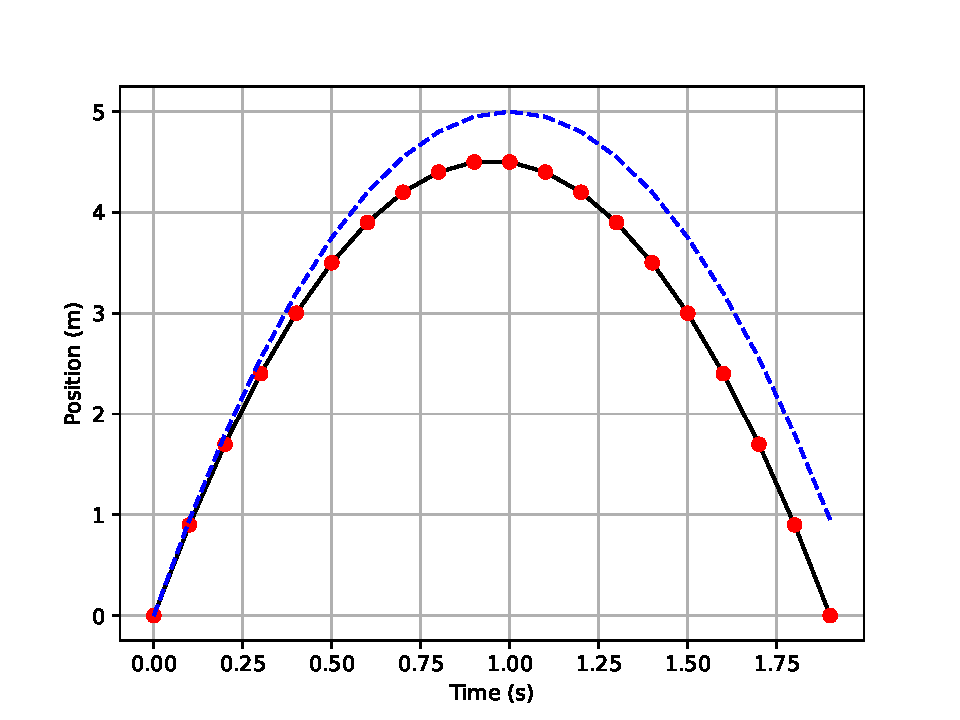
\includegraphics[width=0.8\linewidth]{position}
    \caption{Integración numérica del lanzamiento vertical con $\Delta t = \qty{0.1}{s}$ correspondiente a la línea negra continua con los puntos rojos correspondiente a la integración de cada uno de los 20 pasos, comparado con la solución analítica mostrado en la línea azul a trazos.  }
    \label{fig:vertical}
\end{figure}

Esto corresponde a reemplazar la coordenada $x$ por la coordenada $y$ en la ecuación de movimiento~\eqref{eq:movimientoparabólico} y  $a = -g$, de modo que
\begin{align}
\label{eq:lanzamiento}
    y(t) =y_0 +  v_0 t - \frac{1}{2}g t^2 \,,
\end{align}
con $y_0=0$ para el movimiento representado por la figure~\ref{fig:vertical}.
Note que dicha ecuación es independiente de la masa del objeto lanzado.


\section{Conservación de la energía}
El teorema de Trabajo y Energía para el problema de lanzamiento vertical hacía arriba desde una altura cero con una velocidad inicial $v_0$, hasta una altura $h$ con una velocidad $v$; se puede escribir usando la ecs.~\eqref{eq:TrabajoEnergía} y \eqref{eq:gravitationalconstantforce}, como
\begin{align*}
    W = -mgh =& \frac{1}{2}mv^2 -\frac{1}{2}m v_0^2\,.
\end{align*}
Reorganizando términos
\begin{align}
\label{eq:work}
    \frac{1}{2}m v_0^2 = \frac{1}{2}mv^2 + mgh\,.
\end{align}

Si definimos la energía potencial de un objeto a una altura $h$ sobre la superficie terrestre como
\begin{align}
    U = mgh\,,
\end{align}
entonces, la energía potencial inicial, $U_0$, a una altura cero, es cero, y definiendo la energía cinética como
\begin{align}
    K = \frac{1}{2}m v^2\,,
\end{align}
podemos reescribir la ec.~\eqref{eq:work} como
\begin{align}
    U_0 + K_0 = U + K\,,
\end{align}
esto quiere decir que la energía mecánica
\begin{align}
    E_{\text{total}} = U + K\,,
\end{align}
se conserva.

Es de anotar que está ecuación es de validez general para fuerzas conservativas, es decir fuerzas que sólo contribuyen a la energía mecánica.

Aplicando el teorema de la conservación de energía al lanzamiento vertical hacía arriba para calcular la altura máxima, $y_{\text{max}}$ bajo la condición que en ese punto la velocidad final sea cero. Si parte desde el origen, la energía potencial es cero y la energía total inicial esta dada en su totalidad  por la energía cinética 
\begin{align}
    E_{\text{total}}^{\text{inicial}} = \frac{1}{2}mv_0^2\,. 
\end{align}
Como en el punto final de altura máxima, $y_{\text{max}}$, la velocidad final es cero, la correspondiente energía cinética final es cero, de modo que toda la energía cinética final se ha convertido en energía potencial tal que
\begin{align}
    E_{\text{total}}^{\text{final}} = mg y_{\text{max}}\,.
\end{align}
Igualando las energías: $E_{\text{total}}^{\text{final}}=E_{\text{total}}^{\text{inicial}}$, tenemos que
\begin{align}
\label{eq:ymax}
    \cancel{m}gy_{\text{max}} =& \frac{1}{2}\cancel{m}v_0^2\nonumber\\
    y_{\text{max}}=&\frac{v_0^2}{2g}\,.
\end{align}

Reemplazando en la ecuación de movimiento~\eqref{eq:lanzamiento}) (con $y_0=0$
\begin{align*}
    &y_{\text{max}}=v_0 t_{\text{pico}}-\frac{1}{2}gt_{\text{pico}}^2\\
    &\frac{v_0^2}{2g}-v_0t_{\text{pico}}+\frac{1}{2}gt_{\text{pico}}^2 =0\\
    &v_0^2-2v_0gt_{\text{pico}} +g^2t_{\text{pico}}^2=0\\
    &(v_0-gt_{\text{pico}})^2=0\,,
\end{align*}
que se anula sí
\begin{align}
\label{eq:tpico}
    v_0-gt_{\text{pico}}=&0\nonumber\\
    t_{\text{pico}}=\frac{v_0}{g}\,.
\end{align}
El tiempo de vuelo es el doble de ese tiempo, pues por conservación de la energía donde toda la energía potencial se vuelve a convertir en su totalidad en energía cinética, el tiempo de bajada es igual al de subida
\begin{equation}
\label{eq:tvuelo}
    t_{\text{vuelo}}=2t_{\text{pico}}=\frac{2v_0}{g}\,.
\end{equation}


\section{Movimiento parabólico}
Ver \href{https://colab.research.google.com/drive/1YMC00LP9HcuapJtmcpAcivhiywmEcPwo?usp=sharing}{Colab notebook}


% --- Inicio del código LaTeX para insertar ---

A continuación se presentan las ecuaciones clave del movimiento parabólico (o de proyectil), expresadas en términos de la magnitud de la velocidad inicial ($v_0$) y el ángulo de lanzamiento ($\theta$). Ver figura~\ref{fig:movimiento_parabolico_ascendente} Estas fórmulas asumen que el punto de lanzamiento y el de aterrizaje están a la misma altura y que la resistencia del aire es despreciable.

% --- Inicio del código LaTeX para insertar ---

\begin{figure}[h!] % El [h!] sugiere a LaTeX que intente colocar la figura "aquí"
    \centering % Centra la figura en la página
    \begin{tikzpicture}[
        scale=1, % Escala general de la figura
        font=\large, % Tamaño de la fuente para las etiquetas
        axis/.style={->, %stealth, 
        thick}, % Estilo para los ejes
        vector/.style={->, %>=stealth, 
        ultra thick}, % Estilo para los vectores
        helpline/.style={dashed, gray} % Estilo para líneas de ayuda
    ]
        % --- Dibujar los ejes y el suelo ---
        \draw[axis] (0,0) -- (8.5,0) node[below] {$x$};
        \draw[axis] (0,0) -- (0,4.5) node[left] {$y$}; % Aumentado un poco para el pico
        \node[below left] at (0,0) {Origen};

        % --- Dibujar la trayectoria parabólica ---
        % La trayectoria está definida por la función y = 2x - 0.25x^2
        \draw[blue, thick, domain=0:8, samples=100] plot (\x, {2*\x - 0.25*\x^2}) node[above right] {Trayectoria};
        
        % --- Definir la posición de la partícula en la trayectoria ---
        % CAMBIO PRINCIPAL: Cambiamos xpos de 6 a 2 para estar en la parte ascendente
        \def\xpos{2} 
        \def\ypos{2*\xpos - 0.25*\xpos^2} % Coordenada y calculada automáticamente
        
        % --- Dibujar la partícula ---
        \shade[ball color=red] (\xpos, \ypos) circle (0.15cm);
        
        % --- Dibujar los vectores de velocidad ---
        % Vector velocidad total (tangente a la trayectoria)
        % La pendiente de la tangente es y'(x) = 2 - 0.5x
        % En x=2, la pendiente es 2 - 0.5*2 = 1. El ángulo es 45 grados.
        \begin{scope}[shift={(\xpos,\ypos)}, rotate=45]
            \draw[vector, green!50!black] (0,0) -- (2,0) node[above] {$\boldsymbol{v}$};
        \end{scope}

        % Componente horizontal de la velocidad (vx)
        \draw[vector, green!50!black] (\xpos, \ypos) -- (\xpos + 1.414, \ypos) node[below] {${v}_x=v_{x0}$};

        % Componente vertical de la velocidad (vy)
        \draw[vector, green!50!black] (\xpos, \ypos) -- (\xpos, \ypos + 1.414) node[left] {${v}_y$};

        % Líneas de ayuda para mostrar la composición de vectores
        \draw[helpline] (\xpos + 1.414, \ypos) -- (\xpos + 1.414, \ypos + 1.414);
        \draw[helpline] (\xpos, \ypos + 1.414) -- (\xpos + 1.414, \ypos + 1.414);
        
        % --- Dibujar el vector Fuerza Gravitacional ---
        % Desplazado a la izquierda para mejor visibilidad
        \draw[vector, red] (\xpos, \ypos) -- (\xpos, \ypos - 1.5) node[right] {$\boldsymbol{F} = (0,-mg)$};
        
        % --- Mostrar el vector velocidad inicial ---
        \draw[vector, gray] (0,0) -- (1,2) node[above left] {$\boldsymbol{v}_0$};
        % Ángulo de lanzamiento
        \draw (0.5,0) arc (0:63.4:0.5);
        \node at (0.8, 0.25) {$\theta$};

    \end{tikzpicture}
    \caption{Diagrama de cuerpo libre para una partícula en movimiento parabólico. El vector velocidad $\boldsymbol{v}$ tiene una componente vertical ${v}_y$ positiva (hacia arriba) y una componente constante $v_x$, mientras que la fuerza gravitacional $\boldsymbol{F}$ sigue actuando constantemente hacia abajo.}
    \label{fig:movimiento_parabolico_ascendente}
\end{figure}

\subsection*{Configuración Inicial}
\begin{itemize}
    \item \textbf{Velocidad Inicial (magnitud):} $v_0$
    \item \textbf{Ángulo de Lanzamiento:} $\theta$ (medido desde la horizontal)
    \item \textbf{Aceleración debida a la Gravedad:} $g$ (considerada como un valor positivo, $\approx \SI{9.8}{\meter\per\second\squared}$)
    \item \textbf{Posición Inicial:} $(x_0, y_0) = (0, 0)$
\end{itemize}

\subsection*{Componentes de la Velocidad Inicial}
El vector de velocidad inicial se descompone en sus componentes horizontal ($v_{x0}$) y vertical ($v_{y0}$):
\begin{equation}
    \boxed{v_{x0} = v_0 \cos\theta}
\end{equation}
\begin{equation}
    \boxed{v_{y0} = v_0 \sin\theta}
\end{equation}

\subsection*{Ecuaciones de la Velocidad en función del Tiempo, $t$}
Estas ecuaciones describen las componentes de la velocidad en cualquier instante $t$.

\paragraph{Velocidad Horizontal ($v_x$):}
La velocidad horizontal es constante.
\begin{equation}
    \boxed{v_x(t) = v_0 \cos\theta}
\end{equation}

\paragraph{Velocidad Vertical ($v_y$):}
La velocidad vertical cambia debido a la aceleración gravitacional.
\begin{equation}
    \boxed{v_y(t) = v_0 \sin\theta - gt}
\end{equation}

\subsection*{Ecuaciones de la Posición en función del Tiempo, $t$}
Estas son las ecuaciones paramétricas del movimiento que describen las coordenadas $(x, y)$ del proyectil en cualquier instante $t$.

\paragraph{Posición Horizontal ($x$) a velocidad en $x$ constante:}
\begin{equation}
    \boxed{x(t) = (v_0 \cos\theta) t}
\end{equation}

\paragraph{Posición Vertical ($y$), ecuación de movimiento a aceleración constante~\eqref{eq:lanzamiento}:}
\begin{equation}
    \boxed{y(t) = (v_0 \sin\theta) t - \frac{1}{2}gt^2}
\end{equation}

\section*{Ecuación de la Trayectoria ($y$ en función de $x$)}
Esta ecuación describe la forma parabólica del camino del proyectil, eliminando la variable del tiempo. Se obtiene despejando $t$ de la ecuación de $x(t)$
\begin{align}
    t = \frac{x}{v_0\cos\theta}\,,
\end{align}
y sustituyéndola en la ecuación de $y(t)$.
\begin{equation}
    \boxed{
    y(x) = (\tan\theta)x - \left(\frac{g}{2v_0^2\cos^2\theta}\right)x^2
    }
\end{equation}
Esta es una ecuación de la forma $y = Ax - Bx^2$, que es la fórmula matemática de una parábola que se abre hacia abajo.

\subsection*{Resumen en una Tabla}
Ver Tabla~\ref{tab:parabolic_equations} 

\begin{table}[h!]
\centering,
\caption{Resumen de las Ecuaciones del Movimiento Parabólico.}
\label{tab:parabolic_equations}
\renewcommand{\arraystretch}{1.5} % Aumenta el espaciado vertical de las filas
\begin{tabular}{| >{\centering\arraybackslash}m{2.5cm} | >{\centering\arraybackslash}m{5cm} | >{\centering\arraybackslash}m{5cm} |}
\hline
\textbf{Cantidad} & \textbf{Componente Horizontal (x)} & \textbf{Componente Vertical (\subsection*{Resumen en una Tabla}
y)} \\
\hline \hline
\textbf{Aceleración} & $a_x = 0$ & $a_y = -g$ \\
\hline
\textbf{Velocidad ($t$)} & $v_x = v_0 \cos\theta$ & $v_y(t) = v_0 \sin\theta - gt$ \\
\hline
\textbf{Posición ($t$)} & $x(t) = (v_0 \cos\theta) t$ & $y(t) = (v_0 \sin\theta) t - \frac{1}{2}gt^2$ \\
\hline
\textbf{Trayectoria ($y$ vs $x$)} & \multicolumn{2}{c|}{$y(x) = x\tan\theta - \left(\frac{g}{2v_0^2\cos^2\theta}\right)x^2$} \\
\hline
\end{tabular}
\end{table}

Los movimientos en $x$ y $y$ son independientes, el primero corresponde a un movimiento a velocidad constante $v_x=v_0\cos\theta$ y el segundo a un movimiento de caída libre con velocidad inicial $v_{y0}=v_0\sin\theta$.

Por lo tanto, usando la parte de movimiento vertical podemos obtener la altura máxima, el tiempo para alcanzarla y el tiempo de vuelo de las ecuaciones~\eqref{eq:ymax}, \eqref{eq:tpico} y\eqref{eq:tvuelo}
\begin{align}
    y_{\texttt{max}} =& \frac{v_{y0}^2}{2g}=\frac{v_0^2\sin^2\theta}{2g}\\
    t_{\text{pico}} =&\frac{v_{y0}}{g} = \frac{v_0\sin\theta}{g}\\
    t_{\text{vuelo}} =& 2t_{\text{pico}}=\frac{2v_0\sin\theta}{g}\,.
\end{align}

Con el tiempo de vuelo, podemos hallar el alcance del movimiento parabólico, $R$, que es la distancia recorrida hasta regresar al suelo
\begin{align*}
    R=&v_{x0}t_{\text{vuelo}}\\
    =&\frac{2v_0\cos\theta\sin\theta}{g}\,.
\end{align*}
Finalmente, aplicamos la identidad del ángulo doble, $2\sin\theta\cos\theta = \sin(2\theta)$, para obtener la \textbf{fórmula general del alcance}:
\begin{equation}
    \boxed{R = \frac{v_0^2 \sin(2\theta)}{g}}
\end{equation}

\subsection*{Paso 4: Encontrar el Alcance Máximo ($R_{\text{max}}$)}
Para una $v_0$ dada, $R$ es máximo cuando $\sin(2\theta)$ es máximo. El valor máximo de la función seno es \textbf{1}.
\[ \sin(2\theta) = 1 \implies 2\theta = 90^\circ \implies \boxed{\theta = 45^\circ} \]
Sustituyendo $\sin(2\theta)=1$ en la fórmula del alcance, encontramos el valor del \textbf{alcance máximo}:
\begin{equation}
    \boxed{R_{\text{max}} = \frac{v_0^2}{g}}
\end{equation}
% --- Fin del código LaTeX ---
% --- Inicio del código LaTeX para insertar ---

\subsection{Altura Máxima usando Conservación de la Energía}

El principio de conservación de la energía mecánica nos ofrece una forma sumamente elegante y directa de derivar la fórmula de la altura máxima ($H$) en el movimiento parabólico, sin necesidad de recurrir a las ecuaciones paramétricas del tiempo.

Dado que en nuestro modelo ideal despreciamos la resistencia del aire, la única fuerza que realiza trabajo sobre el proyectil una vez lanzado es la fuerza de gravedad. Como la gravedad es una fuerza conservativa, la energía mecánica total del sistema ($E_{\text{total}} = K + U_g$) permanece constante en cualquier punto de la trayectoria.

\subsubsection*{Paso 1: Energía en el Punto de Lanzamiento (Estado Inicial)}
Situamos nuestro nivel de referencia para la energía potencial gravitacional en el suelo ($y_0 = 0$).
\begin{itemize}
    \item \textbf{Energía Potencial Inicial ($U_i$):} Como la altura es cero, $U_i = 0$.
    \item \textbf{Energía Cinética Inicial ($K_i$):} El proyectil es lanzado con una velocidad total $v_0$. Por lo tanto,
    \begin{equation}
        K_i = \frac{1}{2} m v_0^2.
    \end{equation}
\end{itemize}
La energía mecánica total inicial es simplemente
\begin{equation}
    E_i = K_i + U_i = \frac{1}{2} m v_0^2.
    \label{eq:energia_inicial_parabola}
\end{equation}

\subsubsection*{Paso 2: Energía en la Altura Máxima (Estado Final)}
En el punto más alto de la trayectoria ($y = H$), la componente vertical de la velocidad se vuelve cero ($v_y = 0$). \textbf{¡Atención!} Esto no significa que el objeto se detenga. La componente horizontal de la velocidad ($v_x = v_0 \cos\theta$) permanece constante durante todo el vuelo.
\begin{itemize}
    \item \textbf{Energía Potencial Final ($U_f$):} A una altura $H$, la energía es
    \begin{equation}
        U_f = mgH.
    \end{equation}
    \item \textbf{Energía Cinética Final ($K_f$):} Dado que la única velocidad que tiene el proyectil en la cima es la horizontal, su velocidad total en ese instante es $v_f = v_0 \cos\theta$. La energía cinética será
    \begin{equation}
        K_f = \frac{1}{2} m (v_0 \cos\theta)^2 = \frac{1}{2} m v_0^2 \cos^2\theta.
    \end{equation}
\end{itemize}
La energía mecánica total en la cima es
\begin{equation}
    E_f = K_f + U_f = \frac{1}{2} m v_0^2 \cos^2\theta + mgH.
    \label{eq:energia_final_parabola}
\end{equation}

\subsubsection*{Paso 3: Igualar y Resolver (Álgebra y Trigonometría)}
Por el principio de conservación de la energía, igualamos el estado inicial (\ref{eq:energia_inicial_parabola}) con el estado final (\ref{eq:energia_final_parabola}):
\begin{equation}
    \frac{1}{2} m v_0^2 = \frac{1}{2} m v_0^2 \cos^2\theta + mgH.
\end{equation}
Notamos inmediatamente que la masa ($m$) aparece en todos los términos de la ecuación, por lo que podemos cancelarla dividiendo toda la expresión por $m$. Esto confirma que la trayectoria de caída libre es independiente de la masa del objeto:
\begin{equation}
    \frac{1}{2} v_0^2 = \frac{1}{2} v_0^2 \cos^2\theta + gH.
\end{equation}
Nuestro objetivo es despejar la altura máxima $H$. Primero, pasamos el término de la energía cinética restante al lado izquierdo restando:
\begin{equation}
    gH = \frac{1}{2} v_0^2 - \frac{1}{2} v_0^2 \cos^2\theta.
\end{equation}
Factorizamos el término común $\frac{1}{2} v_0^2$ en el lado derecho:
\begin{equation}
    gH = \frac{1}{2} v_0^2 \left( 1 - \cos^2\theta \right).
\end{equation}
Aquí entra en juego la identidad trigonométrica fundamental ($\sin^2\theta + \cos^2\theta = 1$), de la cual deducimos que $1 - \cos^2\theta = \sin^2\theta$. Sustituyendo esto en nuestra ecuación:
\begin{equation}
    gH = \frac{1}{2} v_0^2 \sin^2\theta.
\end{equation}
Finalmente, dividimos por la aceleración de la gravedad $g$ para obtener la ecuación de la altura máxima:
\begin{equation}
    H = \frac{v_0^2 \sin^2\theta}{2g}.
\end{equation}

\textbf{Conclusión:} 
Hemos recuperado exactamente la misma fórmula que derivamos anteriormente mediante cinemática (Ecuación 3.48). Este método demuestra la profunda consistencia interna de la física: ya sea que analicemos el problema rastreando fuerzas y tiempos (Newton) o rastreando el intercambio entre movimiento y altura (Energía), el universo nos entrega siempre la misma verdad inmutable.

\subsubsection{La rápidez sólo depende de la altura}
Como la energía se conserva, para cualquier punto de la trayectoria tenemos
\begin{align}
    \frac{1}{2}m v_0^2=&\frac{1}{2}m v^2 + mgy\nonumber\\
    \frac{1}{2}v^2 =&\frac{1}{2} v_0^2 - gy\nonumber\\
    v^2 =& v_0^2 - 2gy\nonumber\\
    v(y)=&\sqrt{v_0^2-2gy}\,.
\end{align}


% --- Inicio del código LaTeX para insertar ---

% --- Inicio del código LaTeX para insertar ---


\section{Conservación de la Cantidad de Movimiento}

Así como el Teorema del Trabajo y la Energía nos condujo al principio de conservación de la energía mecánica (un enfoque escalar basado en distancias y cuadrados de velocidades), las Leyes de Newton nos proporcionan una segunda gran ley de conservación, esta vez de naturaleza vectorial: la \textbf{conservación de la cantidad de movimiento} (o momento lineal).

Mientras que la energía es útil para relacionar velocidades con alturas o posiciones, la cantidad de movimiento es la herramienta matemática por excelencia para analizar interacciones directas, explosiones y colisiones entre objetos.

\subsubsection{El Sistema Aislado y la Tercera Ley de Newton}

Consideremos un sistema aislado compuesto por dos partículas de masas $m_1$ y $m_2$. Decir que el sistema está ``aislado'' significa que la suma de las fuerzas externas que actúan sobre ambas partículas es cero ($\boldsymbol{F}_{\text{ext}} = \boldsymbol{0}$). Las únicas fuerzas presentes son las fuerzas internas de interacción entre ellas.

Supongamos que las partículas chocan o interactúan durante un intervalo de tiempo $\Delta t$. Según la \textbf{Tercera Ley de Newton} (Acción y Reacción), la fuerza que la partícula 1 ejerce sobre la partícula 2 ($\boldsymbol{F}_{12}$) es exactamente igual en magnitud y opuesta en dirección a la fuerza que la partícula 2 ejerce sobre la partícula 1 ($\boldsymbol{F}_{21}$):
\begin{equation}
    \boldsymbol{F}_{12} = -\boldsymbol{F}_{21}.
    \label{eq:tercera_ley}
\end{equation}

\subsubsection{Derivación Algebraica del Principio de Conservación}

Recordemos la forma original de la \textbf{Segunda Ley de Newton} (Ecuación 3.1), que establece que una fuerza neta es igual a la tasa de cambio del momento lineal:
\begin{equation}
    \boldsymbol{F} = \frac{\Delta \boldsymbol{p}}{\Delta t}.
\end{equation}

Aplicamos esta definición a cada partícula en nuestra ecuación de acción y reacción (\ref{eq:tercera_ley}). La fuerza $\boldsymbol{F}_{12}$ causa el cambio de momento en la partícula 2 ($\Delta \boldsymbol{p}_2$), y la fuerza $\boldsymbol{F}_{21}$ causa el cambio de momento en la partícula 1 ($\Delta \boldsymbol{p}_1$):
\begin{equation}
    \frac{\Delta \boldsymbol{p}_2}{\Delta t} = - \frac{\Delta \boldsymbol{p}_1}{\Delta t}.
\end{equation}

Dado que la interacción ocurre exactamente durante el mismo intervalo de tiempo $\Delta t$ para ambas partículas, podemos multiplicar ambos lados de la ecuación por $\Delta t$ para cancelarlo algebraicamente:
\begin{equation}
    \Delta \boldsymbol{p}_2 = - \Delta \boldsymbol{p}_1.
\end{equation}

Reorganizamos la ecuación sumando $\Delta \boldsymbol{p}_1$ a ambos lados:
\begin{equation}
    \Delta \boldsymbol{p}_1 + \Delta \boldsymbol{p}_2 = \boldsymbol{0}.
    \label{eq:cambio_momento_cero}
\end{equation}
La Ecuación (\ref{eq:cambio_momento_cero}) nos dice que el \textit{cambio total} en el momento del sistema es cero. Para ver esto de forma más explícita, expandimos los términos de cambio ($\Delta \boldsymbol{p} = \boldsymbol{p}_f - \boldsymbol{p}_i$) para el estado inicial ($i$) y final ($f$):
\begin{equation}
    (\boldsymbol{p}_{1f} - \boldsymbol{p}_{1i}) + (\boldsymbol{p}_{2f} - \boldsymbol{p}_{2i}) = \boldsymbol{0}.
\end{equation}


Reorganizamos los términos, agrupando los momentos iniciales a un lado de la igualdad y los momentos finales al otro:
\begin{equation}
    \boldsymbol{p}_{1i} + \boldsymbol{p}_{2i} = \boldsymbol{p}_{1f} + \boldsymbol{p}_{2f}.
    \label{eq:conservacion_momento}
\end{equation}

Si definimos la \textbf{cantidad de movimiento total del sistema} como $\boldsymbol{P}_{\text{total}} = \boldsymbol{p}_1 + \boldsymbol{p}_2$, la ecuación anterior se resume de manera elegantemente simple:
\begin{equation}
    \boldsymbol{P}_{\text{total}, i} = \boldsymbol{P}_{\text{total}, f}.
\end{equation}

\textbf{Conclusión:}
Hemos demostrado de forma puramente algebraica que, en ausencia de fuerzas externas netas, la cantidad de movimiento total de un sistema aislado se mantiene constante antes, durante y después de cualquier interacción. Las fuerzas internas solo pueden transferir momento de un objeto a otro, pero nunca pueden alterar la cantidad de movimiento total del universo que las contiene.

\subsection{Generalización a Sistemas de Múltiples Partículas: El Centro de Masas}

Considere cualquier sistema aislado compuesto por un número $N$ de partículas (como un cúmulo de estrellas, un gas encerrado en una caja o los fragmentos de una explosión).

\subsubsection{La Cantidad de Movimiento Total}

Consideremos un sistema aislado de $N$ partículas, con masas $m_1, m_2, \dots, m_N$ y velocidades $\boldsymbol{v}_1, \boldsymbol{v}_2, \dots, \boldsymbol{v}_N$. La \textbf{masa total} del sistema es simplemente la suma de las masas individuales:
\begin{equation}
    M_{\text{total}} = m_1 + m_2 + \dots + m_N.
\end{equation}

La \textbf{cantidad de movimiento total} del sistema ($\boldsymbol{P}_{\text{total}}$) es la suma vectorial de los momentos de cada partícula:
\begin{equation}
    \boldsymbol{P}_{\text{total}} = \boldsymbol{p}_1 + \boldsymbol{p}_2 + \dots + \boldsymbol{p}_N = m_1\boldsymbol{v}_1 + m_2\boldsymbol{v}_2 + \dots + m_N\boldsymbol{v}_N.
    \label{eq:momento_n_particulas}
\end{equation}

Como el sistema está aislado (la fuerza externa neta es cero), la Primera Ley de Newton garantiza que este vector $\boldsymbol{P}_{\text{total}}$ es una constante universal en el tiempo, sin importar cuán caóticas sean las colisiones o interacciones internas.

\subsubsection{Definición de la Velocidad del Centro de Masas}

En física, definimos un punto matemático ficticio llamado \textbf{Centro de Masas (CM)} que representa el promedio ponderado de la posición de toda la masa del sistema. La velocidad a la que se mueve este punto ($\boldsymbol{v}_{\text{CM}}$) se define dividiendo la cantidad de movimiento total entre la masa total:
\begin{align}
    \boldsymbol{v}_{\text{CM}}=\frac{\boldsymbol{P}_{\text{total}}}{M_{\text{total}}} =  &
\frac{\boldsymbol{p}_1+\boldsymbol{p}_2+\cdots+\boldsymbol{p}_N}{M_{\text{total}}}
    \nonumber\\
    =&\frac{m_1\boldsymbol{v}_1 + m_2\boldsymbol{v}_2 + \dots + m_N\boldsymbol{v}_N}{M_{\text{total}}}.
\end{align}

Si reorganizamos esta ecuación pasando $M_{\text{total}}$ a multiplicar al lado izquierdo, descubrimos una propiedad bellísima de la mecánica newtoniana:
\begin{equation}
    \boldsymbol{P}_{\text{total}} = M_{\text{total}} \boldsymbol{v}_{\text{CM}}.
    \label{eq:momento_cm}
\end{equation}
Esta ecuación nos dice que, sin importar cuán complejo sea el sistema (incluso si son billones de moléculas rebotando), \textbf{todo el sistema se comporta macroscópicamente como si fuera una sola partícula de masa $M_{\text{total}}$ moviéndose a la velocidad $\boldsymbol{v}_{\text{CM}}$}.


\subsubsection{El Sistema de Referencia del Centro de Masas}

 ¿Qué sucede si decidimos observar nuestro sistema de $N$ partículas desde un sistema de referencia $S'$ que viaja exactamente a la misma velocidad y en la misma dirección que el Centro de Masas?

En este nuevo sistema de referencia, que llamaremos el \textit{Sistema del Centro de Masas}, aplicamos la relatividad de Galileo. La velocidad de cada partícula vista por nuestro observador que se mueve con el centro de masa ($\boldsymbol{v}'_i$) será la velocidad original menos la velocidad del observador que es justo la $\boldsymbol{v}_{\text{CM}}$:
\begin{equation}
    \boldsymbol{v}'_i = \boldsymbol{v}_i - \boldsymbol{v}_{\text{CM}}.
\end{equation}

Calculemos ahora la cantidad de movimiento total en este nuevo sistema de referencia ($\boldsymbol{P}'_{\text{total}}$):
\begin{equation}
    \boldsymbol{P}'_{\text{total}} = m_1\boldsymbol{v}'_1 + m_2\boldsymbol{v}'_2 + \dots + m_N\boldsymbol{v}'_N.
\end{equation}
Sustituyendo nuestras velocidades relativas:
\begin{equation}
    \boldsymbol{P}'_{\text{total}} = m_1(\boldsymbol{v}_1 - \boldsymbol{v}_{\text{CM}}) + m_2(\boldsymbol{v}_2 - \boldsymbol{v}_{\text{CM}}) + \dots + m_N(\boldsymbol{v}_N - \boldsymbol{v}_{\text{CM}}).
\end{equation}
Expandimos los paréntesis algebraicamente:
\begin{equation}
    \boldsymbol{P}'_{\text{total}} = (m_1\boldsymbol{v}_1 + m_2\boldsymbol{v}_2 + \dots + m_N\boldsymbol{v}_N) - (m_1\boldsymbol{v}_{\text{CM}} + m_2\boldsymbol{v}_{\text{CM}} + \dots + m_N\boldsymbol{v}_{\text{CM}}).
\end{equation}
Notamos dos cosas fundamentales. El primer gran paréntesis es, por definición (Ecuación \ref{eq:momento_n_particulas}), el momento total original $\boldsymbol{P}_{\text{total}}$. En el segundo paréntesis, podemos factorizar la velocidad constante $\boldsymbol{v}_{\text{CM}}$:
\begin{equation}
    \boldsymbol{P}'_{\text{total}} = \boldsymbol{P}_{\text{total}} - (m_1 + m_2 + \dots + m_N)\boldsymbol{v}_{\text{CM}}.
\end{equation}
Reconociendo que la suma de las masas es $M_{\text{total}}$, obtenemos:
\begin{equation}
    \boldsymbol{P}'_{\text{total}} = \boldsymbol{P}_{\text{total}} - M_{\text{total}}\boldsymbol{v}_{\text{CM}}.
\end{equation}
Finalmente, usando la Ecuación (\ref{eq:momento_cm}) que nos dice que $\boldsymbol{P}_{\text{total}} = M_{\text{total}}\boldsymbol{v}_{\text{CM}}$, llegamos a la demostración definitiva:
\begin{equation}
    \boldsymbol{P}'_{\text{total}} = \boldsymbol{P}_{\text{total}} - \boldsymbol{P}_{\text{total}} = \boldsymbol{0}.
\end{equation}

\textbf{Conclusión Física:}
Hemos demostrado mediante álgebra que, si observamos \textit{cualquier} sistema de partículas desde la perspectiva de su Centro de Masas, \textbf{la cantidad de movimiento total del sistema será siempre exactamente cero}. 

Por esta razón, a este sistema de referencia se le conoce en la literatura científica como el \textbf{Sistema de Momento Cero} (\textit{Zero-Momentum Frame}). Es la herramienta analítica más poderosa en física de colisiones (incluyendo la física de partículas en aceleradores como el LHC), ya que elimina de las ecuaciones todo el movimiento de traslación irrelevante, dejando a la vista únicamente la física pura de las interacciones internas.

\subsubsection*{Nota Aclaratoria: Conservación vs. Momento Nulo}

Es muy común y lógico preguntarse: \textit{¿No podíamos deducir esto más fácil usando la Primera Ley de Newton? Si la fuerza neta es cero, el cambio de momento es cero ($\Delta \boldsymbol{P} = \boldsymbol{0}$)}.

Es fundamental distinguir entre dos conceptos físicos distintos:
\begin{enumerate}
    \item \textbf{La Conservación del Momento ($\Delta \boldsymbol{P}_{\text{total}} = \boldsymbol{0}$):} Las Leyes de Newton nos garantizan que, en un sistema aislado, la cantidad de movimiento total es una \textbf{constante}. Si observas un choque de asteroides desde la Tierra, el momento total antes y después del choque podría ser una constante inmensa, digamos $\boldsymbol{P}_{\text{total}} = 5000 \text{ kg}\cdot\text{m/s}$. La Ley de Newton te asegura que ese $5000$ no cambiará, pero no lo hace cero.
    
    \item \textbf{El Momento Nulo ($\boldsymbol{P}'_{\text{total}} = \boldsymbol{0}$):} La derivación algebraica que acabamos de realizar demuestra algo diferente. Demuestra que, sin importar cuál sea esa constante desde el punto de vista de la Tierra, \textbf{siempre existe un sistema de referencia particular} (el Sistema del Centro de Masas) donde el valor de esa constante es \textbf{exactamente cero}.
\end{enumerate}

Para entenderlo con una analogía cotidiana: imagina que estás dentro de un tren que viaja a velocidad constante. 
\begin{itemize}
    \item Para alguien parado en la estación, tú y tus maletas tienen una cantidad de movimiento enorme que se conserva constante ($\Delta \boldsymbol{P} = \boldsymbol{0}$). 
    \item Pero si analizamos la física desde tu asiento dentro del tren (tu centro de masas), tú y tus maletas están quietos. La cantidad de movimiento en ese sistema de referencia no solo se conserva, sino que es \textbf{nula} ($\boldsymbol{P}' = \boldsymbol{0}$).
\end{itemize}

El Sistema del Centro de Masas es el equivalente matemático a ``subirnos al tren'' del universo para que las ecuaciones de colisiones sean muchísimo más fáciles de resolver.

\subsection{Demostración Algebraica de la Posición del Centro de Masas}

En las secciones anteriores, definimos el Centro de Masas (CM) a partir de su estado dinámico, estableciendo que su velocidad ($\boldsymbol{v}_{\text{CM}}$) es el promedio ponderado de las velocidades de todas las partículas para garantizar que $\boldsymbol{P}_{\text{total}} = M_{\text{total}} \boldsymbol{v}_{\text{CM}}$. Pero, ¿de dónde surge la fórmula para encontrar su \textit{posición} exacta ($\boldsymbol{r}_{\text{CM}}$) en el espacio?

A continuación, demostraremos que la fórmula geométrica de la posición es una consecuencia cinemática ineludible de nuestra definición de la cantidad de movimiento, utilizando únicamente álgebra básica.

\subsubsection{Paso 1: La Definición de la Velocidad del CM}

Partimos de la ecuación que define la velocidad del Centro de Masas para un sistema de $N$ partículas:
\begin{equation}
    \boldsymbol{v}_{\text{CM}} = \frac{m_1\boldsymbol{v}_1 + m_2\boldsymbol{v}_2 + \dots + m_N\boldsymbol{v}_N}{M_{\text{total}}}.
    \label{eq:v_cm_demo}
\end{equation}

\subsubsection{Paso 2: Relación Cinemática entre Velocidad y Posición}

Sabemos por la cinemática fundamental que la velocidad constante o promedio de cualquier objeto es igual a su cambio de posición (desplazamiento, $\Delta\boldsymbol{r}$) dividido por el intervalo de tiempo transcurrido ($\Delta t$):
\begin{equation}
    \boldsymbol{v} = \frac{\Delta \boldsymbol{r}}{\Delta t}.
\end{equation}
Sustituimos esta definición cinemática geométrica para cada una de las velocidades en la Ecuación (\ref{eq:v_cm_demo}), tanto para el Centro de Masas en el lado izquierdo, como para cada partícula individual en el lado derecho:
\begin{equation}
    \frac{\Delta \boldsymbol{r}_{\text{CM}}}{\Delta t} = \frac{m_1\left(\frac{\Delta \boldsymbol{r}_1}{\Delta t}\right) + m_2\left(\frac{\Delta \boldsymbol{r}_2}{\Delta t}\right) + \dots + m_N\left(\frac{\Delta \boldsymbol{r}_N}{\Delta t}\right)}{M_{\text{total}}}.
\end{equation}

\subsubsection{Paso 3: Simplificación del Tiempo}

Dado que estamos analizando el movimiento de todo el sistema de manera simultánea durante el mismo intervalo de tiempo exacto $\Delta t$, podemos factorizar el término $\frac{1}{\Delta t}$ en el numerador del lado derecho:
\begin{equation}
    \frac{\Delta \boldsymbol{r}_{\text{CM}}}{\Delta t} = \frac{\frac{1}{\Delta t} \big( m_1\Delta \boldsymbol{r}_1 + m_2\Delta \boldsymbol{r}_2 + \dots + m_N\Delta \boldsymbol{r}_N \big)}{M_{\text{total}}}.
\end{equation}
Multiplicamos ambos lados de la igualdad por $\Delta t$, lo que nos permite cancelar algebraicamente el tiempo de la ecuación. Obtenemos así una relación exclusiva para los desplazamientos:
\begin{equation}
    \Delta \boldsymbol{r}_{\text{CM}} = \frac{m_1\Delta \boldsymbol{r}_1 + m_2\Delta \boldsymbol{r}_2 + \dots + m_N\Delta \boldsymbol{r}_N}{M_{\text{total}}}.
    \label{eq:desplazamiento_cm}
\end{equation}

\subsubsection{Paso 4: Del Desplazamiento a la Posición Absoluta}

La Ecuación (\ref{eq:desplazamiento_cm}) nos dice cómo cambia la posición del Centro de Masas en función de cómo cambian las posiciones individuales. Sabemos por definición que cualquier desplazamiento es la posición final menos la posición inicial ($\Delta \boldsymbol{r} = \boldsymbol{r}_f - \boldsymbol{r}_i$). 

Sustituyamos esta definición explícita para cada uno de los desplazamientos en nuestra ecuación:
\begin{equation}
    \boldsymbol{r}_{\text{CM},f} - \boldsymbol{r}_{\text{CM},i} = \frac{m_1(\boldsymbol{r}_{1f} - \boldsymbol{r}_{1i}) + m_2(\boldsymbol{r}_{2f} - \boldsymbol{r}_{2i}) + \dots + m_N(\boldsymbol{r}_{Nf} - \boldsymbol{r}_{Ni})}{M_{\text{total}}}.
\end{equation}

Ahora, utilizamos el álgebra distributiva para separar las posiciones finales de las iniciales en el numerador:
\begin{equation}
    \boldsymbol{r}_{\text{CM},f} - \boldsymbol{r}_{\text{CM},i} = \frac{(m_1\boldsymbol{r}_{1f} + \dots + m_N\boldsymbol{r}_{Nf}) - (m_1\boldsymbol{r}_{1i} + \dots + m_N\boldsymbol{r}_{Ni})}{M_{\text{total}}}.
\end{equation}

Podemos separar esta gran fracción en la resta de dos fracciones independientes:
\begin{equation}
    \boldsymbol{r}_{\text{CM},f} - \boldsymbol{r}_{\text{CM},i} = \left( \frac{m_1\boldsymbol{r}_{1f} + \dots + m_N\boldsymbol{r}_{Nf}}{M_{\text{total}}} \right) - \left( \frac{m_1\boldsymbol{r}_{1i} + \dots + m_N\boldsymbol{r}_{Ni}}{M_{\text{total}}} \right).
\end{equation}

Observemos cuidadosamente la estructura de esta ecuación. El lado izquierdo es la resta del estado final menos el estado inicial del Centro de Masas. El lado derecho es exactamente la misma operación matemática, separada en un bloque evaluado con las variables finales y otro bloque idéntico evaluado con las variables iniciales. 

Para que esta igualdad se mantenga cierta para \textit{cualquier} intervalo de tiempo y \textit{cualquier} configuración inicial de las partículas, la estructura matemática que define la posición en un instante dado debe corresponder exactamente a los términos entre paréntesis. Igualando el estado final con el final (o el inicial con el inicial), deducimos ineludiblemente la fórmula general y absoluta para la posición del Centro de Masas en cualquier instante de tiempo:
\begin{equation}
    \boldsymbol{r}_{\text{CM}} = \frac{m_1\boldsymbol{r}_1 + m_2\boldsymbol{r}_2 + \dots + m_N\boldsymbol{r}_N}{M_{\text{total}}}.
\end{equation}

\textbf{Conclusión Física:}
Esta demostración revela que la fórmula del Centro de Masas no es una definición estática arbitraria, sino la consecuencia directa de exigir que la dinámica del sistema (su cantidad de movimiento total) sea perfectamente coherente con su cinemática geométrica, sin importar dónde se encontraban las partículas originalmente. El Centro de Masas es el único punto geométrico en el espacio cuya trayectoria imita a la perfección a una partícula que poseyera toda la masa del sistema.

Si sobre el sistema de $N$ partículas hay una Fuerza externa neta que actua sobre todas ellas, cómo la fuerza de la gravedad en la explosión de una granada, ecuación fundamental que relaciona la fuerza neta con la cantidad de movimiento total y el Centro de Masas es la primera primera Ley de Newton~\eqref{eq:newton} que ahora ve todo el sistema cómo un único en la posición del centro de masa en el cual está concentrada la masa toda del sistema
\begin{equation}
\label{eq:newtonN}
    \boldsymbol{F}_{\text{neta, ext}} = \frac{\Delta \boldsymbol{P}_{\text{total}}}{\Delta t} = M_{\text{total}} \boldsymbol{a}_{\text{CM}}.
\end{equation}
donde $\boldsymbol{a}_{\text{CM}}$ es la aceleración del centro de masa, que en el caso de una aceleración constante corresponde a
\begin{equation}
    \boldsymbol{a}_{\text{CM}} = \frac{\boldsymbol{v}_{\text{CM}}}{\Delta t}\,.
\end{equation}

\subsubsection{Ejemplo Analítico: Colisión Totalmente Inelástica}

Para ilustrar el poder de este principio, analizaremos el caso de una colisión totalmente inelástica, que ocurre cuando dos objetos chocan y quedan unidos, moviéndose juntos como un solo cuerpo después del impacto.

\textbf{El Problema:} Un vagón de tren de masa $m_1$ que viaja a una velocidad inicial $v_1$ choca y se acopla mecánicamente a un segundo vagón de masa $m_2$ que se encontraba en reposo ($v_2 = 0$). ¿Cuál es la velocidad final $v_f$ de ambos vagones unidos justo después del choque?

\textbf{Solución:}
Aplicamos el principio de conservación de la cantidad de movimiento. Como todo el movimiento ocurre en una sola dimensión (la vía del tren), podemos prescindir de la notación vectorial y usar los signos para indicar la dirección.

1. Identificamos el momento inicial total del sistema:
\begin{equation}
    P_i = p_{1i} + p_{2i} = m_1 v_1 + m_2 (0) = m_1 v_1.
\end{equation}

2. Identificamos el momento final total del sistema. Al quedar unidos, ambos vagones comparten la misma velocidad final $v_f$ y su masa combinada es $(m_1 + m_2)$:
\begin{equation}
    P_f = (m_1 + m_2) v_f.
\end{equation}

3. Igualamos el momento inicial y el final ($P_i = P_f$):
\begin{equation}
    m_1 v_1 = (m_1 + m_2) v_f.
\end{equation}

4. Despejamos algebraicamente la velocidad final $v_f$:
\begin{equation}
    v_f = \left( \frac{m_1}{m_1 + m_2} \right) v_1.
\end{equation}

Este resultado algebraico nos muestra inmediatamente que, al aumentar la masa total del sistema en movimiento (el denominador es mayor que el numerador), la velocidad final inevitablemente será menor que la velocidad inicial del primer vagón. La cantidad de movimiento se ha distribuido perfectamente entre ambos objetos.

\subsubsection{Ejemplo Analítico: Colisión Elástica en Una Dimensión}

A diferencia de una colisión inelástica (donde la energía cinética se transforma parcialmente en calor o deformación), una \textbf{colisión elástica} es un choque idealizado en el que se conservan simultáneamente dos cantidades fundamentales: la cantidad de movimiento y la energía cinética mecánica. Este modelo describe de forma excelente las colisiones entre bolas de billar o entre partículas subatómicas.

\textbf{El Problema:} Una partícula de masa $m_1$ viaja a una velocidad inicial $v_{1i}$ y choca frontalmente de forma perfectamente elástica contra una segunda partícula de masa $m_2$ que se encuentra inicialmente en reposo ($v_{2i} = 0$). Queremos encontrar las fórmulas algebraicas para las velocidades finales de ambas partículas ($v_{1f}$ y $v_{2f}$).

\textbf{Solución:}
Tenemos dos incógnitas ($v_{1f}$ y $v_{2f}$), por lo que necesitamos plantear un sistema de dos ecuaciones basadas en nuestros principios de conservación.

1. \textbf{Conservación de la cantidad de movimiento:}
\begin{equation}
    m_1 v_{1i} = m_1 v_{1f} + m_2 v_{2f}.
\end{equation}
Agrupamos los términos de la masa 1 en el lado izquierdo y factorizamos:
\begin{equation}
    m_1 (v_{1i} - v_{1f}) = m_2 v_{2f}.
    \label{eq:momento_elastico}
\end{equation}

2. \textbf{Conservación de la energía cinética:}
\begin{equation}
    \frac{1}{2}m_1 v_{1i}^2 = \frac{1}{2}m_1 v_{1f}^2 + \frac{1}{2}m_2 v_{2f}^2.
\end{equation}
Multiplicamos toda la ecuación por 2 para eliminar las fracciones, agrupamos los términos de $m_1$ a la izquierda y factorizamos:
\begin{equation}
    m_1 (v_{1i}^2 - v_{1f}^2) = m_2 v_{2f}^2.
\end{equation}
Aquí aplicamos una herramienta algebraica fundamental: la \textbf{diferencia de cuadrados} ($A^2 - B^2 = (A-B)(A+B)$). Nuestra ecuación de energía se transforma en:
\begin{equation}
    m_1 (v_{1i} - v_{1f})(v_{1i} + v_{1f}) = m_2 v_{2f}^2.
    \label{eq:energia_elastica}
\end{equation}

3. \textbf{El truco algebraico:} 
Para resolver este sistema de forma elegante, dividimos la ecuación de energía (\ref{eq:energia_elastica}) entre la ecuación de momento (\ref{eq:momento_elastico}):
\begin{equation}
    \frac{m_1 (v_{1i} - v_{1f})(v_{1i} + v_{1f})}{m_1 (v_{1i} - v_{1f})} = \frac{m_2 v_{2f}^2}{m_2 v_{2f}}.
\end{equation}
Casi todos los términos se cancelan mágicamente, dejándonos con una relación lineal extremadamente simple:
\begin{equation}
    v_{1i} + v_{1f} = v_{2f}.
    \label{eq:velocidad_relativa}
\end{equation}

4. \textbf{Despejar las velocidades finales:}
Ahora podemos usar la Ecuación (\ref{eq:velocidad_relativa}) para sustituir $v_{2f}$ en nuestra primera ecuación de momento original ($m_1 v_{1i} = m_1 v_{1f} + m_2 v_{2f}$):
\begin{equation}
    m_1 v_{1i} = m_1 v_{1f} + m_2 (v_{1i} + v_{1f}).
\end{equation}
Expandimos y agrupamos los términos que contienen $v_{1f}$ a un lado, y los que contienen $v_{1i}$ al otro:
\begin{equation}
    m_1 v_{1i} - m_2 v_{1i} = m_1 v_{1f} + m_2 v_{1f},
\end{equation}
\begin{equation}
    (m_1 - m_2)v_{1i} = (m_1 + m_2)v_{1f}.
\end{equation}
Despejamos finalmente $v_{1f}$:
\begin{equation}
    v_{1f} = \left( \frac{m_1 - m_2}{m_1 + m_2} \right) v_{1i}.
    \label{eq:v1f_elastica}
\end{equation}

Para encontrar $v_{2f}$, sustituimos el resultado de (\ref{eq:v1f_elastica}) en la ecuación (\ref{eq:velocidad_relativa}) ($v_{2f} = v_{1i} + v_{1f}$):
\begin{equation}
    v_{2f} = v_{1i} + \left( \frac{m_1 - m_2}{m_1 + m_2} \right) v_{1i} = \left( \frac{m_1 + m_2 + m_1 - m_2}{m_1 + m_2} \right) v_{1i},
\end{equation}
lo que se simplifica a:
\begin{equation}
    v_{2f} = \left( \frac{2m_1}{m_1 + m_2} \right) v_{1i}.
    \label{eq:v2f_elastica}
\end{equation}

\textbf{Interpretación Física de los Casos Límite:}
Las fórmulas obtenidas nos permiten predecir el comportamiento del universo en situaciones extremas:
\begin{itemize}
    \item \textbf{Masas iguales ($m_1 = m_2$):} Si las bolas de billar son idénticas, las ecuaciones dictan que $v_{1f} = 0$ y $v_{2f} = v_{1i}$. La primera bola se detiene por completo y transfiere \textit{toda} su velocidad y momento a la segunda bola.
    \item \textbf{Un vehículo pesado choca contra un objeto ligero ($m_1 \gg m_2$):} Si $m_1$ es infinitamente más grande, $m_2$ se vuelve despreciable en las fracciones. El resultado es $v_{1f} \approx v_{1i}$ (el objeto pesado casi no siente el impacto) y $v_{2f} \approx 2v_{1i}$ (el objeto ligero sale disparado al doble de la velocidad del objeto pesado).
    \item \textbf{Un objeto ligero choca contra una pared inamovible ($m_1 \ll m_2$):} Aquí, $m_1$ se vuelve despreciable. Obtendremos $v_{1f} \approx -v_{1i}$ y $v_{2f} \approx 0$. La pelota ligera simplemente rebota con la misma rapidez en sentido contrario, y la pared ni se inmuta.
\end{itemize}

\subsubsection{Ejemplo Analítico: Sistema Binario bajo Gravedad Mutua}

Hasta ahora hemos analizado colisiones donde el contacto es físico e instantáneo. Sin embargo, la conservación de la cantidad de movimiento aplica a cualquier sistema aislado, sin importar si las fuerzas internas actúan a distancia. Un ejemplo majestuoso de esto es un \textbf{sistema binario} en el espacio (como dos estrellas, o una estrella y un exoplaneta) que interactúan exclusivamente mediante su atracción gravitacional mutua.

\textbf{El Problema:} Consideremos dos cuerpos celestes de masas $m_1$ y $m_2$ aislados en el espacio. Según la Ley de Gravitación Universal de Newton, la fuerza que $m_1$ ejerce sobre $m_2$ es exactamente igual y opuesta a la fuerza que $m_2$ ejerce sobre $m_1$ (un par de acción y reacción). Como no hay fuerzas externas, la cantidad de movimiento total del sistema se conserva. Queremos analizar matemáticamente cómo se mueven estos cuerpos el uno respecto al otro.

\begin{figure}[htbp]
\centering
\begin{tikzpicture}[>=stealth, scale=1.2]
    
    % Centro de Masas
    \coordinate (CM) at (0,0);
    \draw[thick] (-0.1, 0) -- (0.1, 0);
    \draw[thick] (0, -0.1) -- (0, 0.1);
    \node[below, font=\scriptsize] at (CM) {Centro de Masas (CM)};

    % Órbitas
    \draw[dashed, gray] (CM) circle (1.5); % Órbita m1
    \draw[dashed, gray] (CM) circle (3.5); % Órbita m2

    % Masas
    \coordinate (M1) at (-1.5, 0);
    \coordinate (M2) at (3.5, 0);
    
    % Línea que los une
    \draw[thick, gray!80!black] (M1) -- (M2);
    
    % Dibujar Masa 1 (Estrella)
    \draw[thick, fill=yellow!40] (M1) circle (0.4) node {$m_1$};
    \draw[->, ultra thick, red] (M1) -- (-1.5, -1.2) node[left] {$\boldsymbol{v}_1$};
    
    % Dibujar Masa 2 (Planeta)
    \draw[thick, fill=blue!20] (M2) circle (0.2) node {$m_2$};
    \draw[->, ultra thick, blue] (M2) -- (3.5, 1.8) node[right] {$\boldsymbol{v}_2$};

    % Radios
    \draw[<->] (-1.5, 0.2) -- (0, 0.2) node[midway, above] {$r_1$};
    \draw[<->] (0, 0.2) -- (3.5, 0.2) node[midway, above] {$r_2$};

\end{tikzpicture}
\caption{Un sistema binario orbitando su centro de masas común. Las cantidades de movimiento de ambos cuerpos ($\boldsymbol{p}_1$ y $\boldsymbol{p}_2$) son siempre iguales en magnitud y opuestas en dirección, garantizando que el momento total sea cero respecto al CM.}
\label{fig:sistema_binario}
\end{figure}

\textbf{Solución:}
Para simplificar el análisis, los astrofísicos eligen un sistema de referencia que viaja junto con el sistema binario. En este sistema de referencia, llamado \textbf{sistema del Centro de Masas (CM)}, la cantidad de movimiento total del sistema es exactamente cero:
\begin{equation}
    \boldsymbol{P}_{\text{total}} = \boldsymbol{p}_1 + \boldsymbol{p}_2 = \boldsymbol{0}.
\end{equation}
Al despejar algebraicamente, obtenemos una relación directa entre los momentos individuales:
\begin{equation}
    \boldsymbol{p}_1 = -\boldsymbol{p}_2.
\end{equation}
Expandiendo esta ecuación con la definición de momento ($\boldsymbol{p} = m\boldsymbol{v}$), tenemos
\begin{equation}
    m_1 \boldsymbol{v}_1 = - m_2 \boldsymbol{v}_2.
    \label{eq:momento_binario}
\end{equation}
El signo negativo nos indica matemáticamente que, en cualquier instante, las velocidades de ambos cuerpos deben apuntar en \textbf{direcciones opuestas} (ver Figura \ref{fig:sistema_binario}). 

Si analizamos solo las magnitudes (los tamaños de los vectores, ignorando las direcciones), obtenemos:
\begin{equation}
    m_1 v_1 = m_2 v_2.
\end{equation}

Esto significa que la Tierra \textit{no está perfectamente inmóvil respecto a la Luna}. Debido a la conservación de la cantidad de movimiento, La Luna tira de la Tierra y la obliga a describir una pequeña órbita con una pequeña velocidad ($v_1$). 


\subsubsection{Cálculo de la Posición del Centro de Masas en el Sistema Binario}

Vamos a calcular explícitamente la posición de este Centro de Masas (CM) a partir de su definición geométrica formal.

\textbf{Definición General:} La posición del Centro de Masas de un sistema de partículas se define como el promedio de las posiciones de las partículas, ponderado por sus respectivas masas. Para un sistema de dos partículas con masas $m_1$ y $m_2$, y posiciones $\boldsymbol{r}_1$ y $\boldsymbol{r}_2$, el vector de posición del centro de masas $\boldsymbol{r}_{\text{CM}}$ se define algebraicamente como
\begin{equation}
    \boldsymbol{r}_{\text{CM}} = \frac{m_1 \boldsymbol{r}_1 + m_2 \boldsymbol{r}_2}{m_1 + m_2}.
\end{equation}

\textbf{Configuración del Problema (En una dimensión):}
Para simplificar el cálculo sin perder rigor, alinearemos nuestro sistema de coordenadas a lo largo de la línea imaginaria que une a las dos masas. De este modo, podemos prescindir de los vectores y trabajar únicamente con coordenadas en el eje $x$. 

Sea $d$ la distancia total que separa a las dos masas ($d = r_1 + r_2$). Para hacer el álgebra lo más sencilla posible, colocaremos el origen de nuestro sistema de coordenadas exactamente sobre la masa $1$.
\begin{itemize}
    \item Posición de la masa 1: $x_1 = 0$.
    \item Posición de la masa 2: $x_2 = d$.
\end{itemize}

\textbf{Cálculo Algebraico:}
Sustituimos estas coordenadas en nuestra fórmula unidimensional del Centro de Masas:
\begin{equation}
    x_{\text{CM}} = \frac{m_1 (0) + m_2 (d)}{m_1 + m_2}.
\end{equation}
El término $m_1(0)$ se anula, por lo que la posición del Centro de Masas respecto a la masa 1 es
\begin{equation}
    x_{\text{CM}} = \left( \frac{m_2}{m_1 + m_2} \right) d.
    \label{eq:posicion_cm_m1}
\end{equation}

\textbf{Conexión con los Radios Orbitales ($r_1$ y $r_2$):}
Como el Centro de Masas es el punto alrededor del cual orbitan los cuerpos, la distancia desde la masa 1 hasta el Centro de Masas es, por definición, su radio orbital $r_1$. Por lo tanto, de la Ecuación (\ref{eq:posicion_cm_m1}) obtenemos directamente
\begin{equation}
    r_1 = \left( \frac{m_2}{m_1 + m_2} \right) d.
\end{equation}

Para encontrar el radio orbital del segundo cuerpo ($r_2$), es decir, la distancia desde el Centro de Masas hasta la masa 2, simplemente restamos $r_1$ de la distancia total $d$:
\begin{equation}
    r_2 = d - r_1 = d - \left( \frac{m_2}{m_1 + m_2} \right) d.
\end{equation}
Factorizamos $d$ y resolvemos la resta de fracciones:
\begin{equation}
    r_2 = d \left[ 1 - \frac{m_2}{m_1 + m_2} \right] = d \left[ \frac{m_1 + m_2 - m_2}{m_1 + m_2} \right],
\end{equation}
lo que se simplifica hermosamente a
\begin{equation}
    r_2 = \left( \frac{m_1}{m_1 + m_2} \right) d.
\end{equation}

\textbf{Comprobación de Consistencia:}
Si ahora tomamos nuestras expresiones puramente geométricas para $r_1$ y $r_2$ y dividimos la una entre la otra, obtenemos
\begin{equation}
    \frac{r_1}{r_2} = \frac{\left( \frac{m_2}{m_1 + m_2} \right) d}{\left( \frac{m_1}{m_1 + m_2} \right) d}.
\end{equation}
Al cancelar los términos comunes ($d$ y el denominador $m_1 + m_2$), la fracción se reduce a
\begin{equation}
    \frac{r_1}{r_2} = \frac{m_2}{m_1}.
\end{equation}
Multiplicando en cruz recuperamos nuestra famosa relación
\begin{equation}
    m_1 r_1 = m_2 r_2.
\end{equation}

\subsection*{Ejemplo conceptual:  Aniquilación Electrón-Positrón a fotones}

En el capítulo sobre Relatividad Especial, discutimos que cuando una partícula de materia (como un electrón, $e^-$) se encuentra con su antipartícula (un positrón, $e^+$), ambas se aniquilan. Toda su masa se convierte en energía pura en forma de luz (fotones), obedeciendo la relación $E = \Delta m c^2$.

Sin embargo, hay un detalle profundo en este proceso: la aniquilación de un par electrón-positrón \textbf{nunca produce un solo fotón}; siempre produce un mínimo de dos fotones. ¿Por qué el universo prohíbe la creación de un único destello de luz? La respuesta no radica en la energía, sino en una exigencia estricta de la cinemática y la conservación del momento, que se hace evidente al utilizar el concepto del Centro de Masas.

\subsubsection{El Análisis desde el Sistema del Centro de Masas}

Consideremos un electrón y un positrón que colisionan. Como aprendimos en nuestra discusión sobre la dinámica de múltiples partículas, siempre podemos elegir observar este evento desde el \textbf{Sistema del Centro de Masas} (el ``Sistema de Momento Cero''). 

En este sistema de referencia, las dos partículas se acercan mutuamente con cantidades de movimiento exactamente opuestas. Por lo tanto, la cantidad de movimiento total inicial del sistema es estrictamente nula:
\begin{equation}
    \boldsymbol{P}_{\text{inicial}} = \boldsymbol{p}_{e^-} + \boldsymbol{p}_{e^+} = \boldsymbol{0}.
\end{equation}

Como el sistema está aislado (no hay fuerzas externas interactuando con las partículas), la Ley de Conservación de la Cantidad de Movimiento nos exige que el momento total después de la aniquilación siga siendo exactamente cero:
\begin{equation}
    \boldsymbol{P}_{\text{final}} = \boldsymbol{0}.
    \label{eq:momento_final_cero}
\end{equation}

\subsubsection{El Problema de un Solo Fotón}

Supongamos por un momento que la aniquilación produjera un único fotón ($\gamma$). La conservación de la energía se cumpliría perfectamente, ya que el fotón heredaría toda la energía de las masas en reposo ($E_\gamma = 2m_e c^2$). 

No obstante, recordemos la ecuación del momento para partículas sin masa (como derivamos en la Ecuación~\eqref{eq:energiafoton}). Un fotón siempre viaja a la velocidad de la luz y su cantidad de movimiento está atada a su energía:
\begin{equation}
    |\boldsymbol{p}_\gamma| = \frac{E_\gamma}{c}.
\end{equation}

Puesto que el fotón transporta toda la energía de la aniquilación ($E_\gamma \neq 0$), su cantidad de movimiento \textbf{jamás puede ser cero} ($|\boldsymbol{p}_\gamma| \neq 0$). 

Si solo existiera este fotón, el momento total final del sistema sería simplemente el momento de ese fotón:
\begin{equation}
    \boldsymbol{P}_{\text{final}} = \boldsymbol{p}_\gamma \neq \boldsymbol{0}.
\end{equation}
Esto entra en contradicción directa e insalvable con nuestra Ecuación (\ref{eq:momento_final_cero}). Crear un solo fotón violaría la conservación de la cantidad de movimiento. En términos simples: el fotón saldría disparado hacia un lado, llevándose un ``impulso'' que no existía al principio en el Centro de Masas.

\subsubsection{La Solución de la Naturaleza: Dos Fotones}

Para salvar la conservación del momento, el universo debe producir al menos \textbf{dos fotones}. Evaluemos el momento final en este escenario:
\begin{equation}
    \boldsymbol{P}_{\text{final}} = \boldsymbol{p}_{\gamma 1} + \boldsymbol{p}_{\gamma 2} = \boldsymbol{0}.
\end{equation}
Al despejar algebraicamente, obtenemos la condición geométrica que deben cumplir los destellos de luz:
\begin{equation}
    \boldsymbol{p}_{\gamma 1} = -\boldsymbol{p}_{\gamma 2}.
\end{equation}

\textbf{Conclusión Física:}
El álgebra del Centro de Masas nos revela que los dos fotones resultantes de la aniquilación deben tener \textbf{la misma energía} (misma magnitud de momento) y deben salir disparados en \textbf{direcciones exactamente opuestas} (signo negativo en el vector). De esta manera, el ``empuje'' del primer fotón hacia la derecha cancela perfectamente el ``empuje'' del segundo fotón hacia la izquierda, garantizando que el momento total del sistema permanezca en su valor inmutable de cero.





\subsubsection{Ejemplo Conceptual: La Explosión de una Granada en Vuelo}

Una de las consecuencias más espectaculares de la física del Centro de Masas se observa cuando un objeto complejo se rompe o explota en pleno movimiento. 

Imaginemos una granada que es lanzada al aire, describiendo el clásico movimiento parabólico que estudiamos en secciones anteriores. Ver figura~\ref{fig:explosion_granada}. En el punto más alto de su trayectoria, la granada explota violentamente, dividiéndose en decenas de fragmentos que salen disparados en direcciones aparentemente caóticas. ¿Qué sucede con la trayectoria del sistema?

\begin{figure}[htbp]
\centering
\begin{tikzpicture}[scale=1.2, >=stealth]
    
    % Superficie
    \draw[thick, gray!80!black] (-1, 0) -- (9, 0) node[right, text=black] {$x$};
    
    % Trayectoria parabólica original (y = a*x*(x-8) con vértice en (4, 3) -> 3 = a*4*(-4) -> a = -3/16 = -0.1875)
    \draw[dashed, thick, gray] plot[domain=0:8, samples=50] (\x, {-0.1875*\x*(\x - 8)});
    
    % Granada antes de la explosión (ejemplo en x=2)
    \coordinate (G1) at (2, 2.25);
    \draw[fill=green!40!black, thick] (G1) ellipse (0.15 and 0.2);
    \draw[->, thick] (G1) -- (2.8, 3.1) node[above left] {$\boldsymbol{v}$};
    
    % Punto de explosión (Vértice en x=4)
    \coordinate (Exp) at (4, 3);
    \node[starburst, fill=red, draw=yellow, inner sep=2pt, line width=1pt] at (Exp) {};
    
    % Trayectoria del CM DESPUÉS de la explosión
    \draw[dashed, ultra thick, blue!80!black] plot[domain=4:8, samples=50] (\x, {-0.1875*\x*(\x - 8)});
    
    % Posición del CM en un instante posterior (ejemplo en x=6)
    \coordinate (CM) at (6, 2.25);
    \fill[blue, thick] (CM) circle (2pt) node[above right] {$\boldsymbol{r}_{\text{CM}}$};
    
    % Fragmentos aleatorios alrededor del CM en x=6
    % El CM (6, 2.25) debe ser el "promedio" de estos fragmentos
    \coordinate (F1) at (5.0, 3.5);
    \coordinate (F2) at (7.5, 3.0);
    \coordinate (F3) at (4.5, 1.5);
    \coordinate (F4) at (6.5, 1.0);
    
    \fill[gray!70!black] (F1) circle (1.5pt); \draw[->, gray] (Exp) -- (F1);
    \fill[gray!70!black] (F2) circle (2.5pt); \draw[->, gray] (Exp) -- (F2);
    \fill[gray!70!black] (F3) circle (1.0pt); \draw[->, gray] (Exp) -- (F3);
    \fill[gray!70!black] (F4) circle (2.0pt); \draw[->, gray] (Exp) -- (F4);
    
    % Conectar los fragmentos al CM para mostrar el "promedio"
    \draw[dotted, blue!50] (F1) -- (CM);
    \draw[dotted, blue!50] (F2) -- (CM);
    \draw[dotted, blue!50] (F3) -- (CM);
    \draw[dotted, blue!50] (F4) -- (CM);
    
    % Etiquetas
    \node[align=center, font=\small, text=black] at (4, 4) {Explosión\\(Fuerzas Internas)};

\end{tikzpicture}
\caption{Explosión de un proyectil en movimiento parabólico. Aunque los fragmentos individuales (puntos grises) salen disparados en trayectorias complejas, el Centro de Masas del sistema (punto azul) continúa describiendo exactamente la misma parábola original.}
\label{fig:explosion_granada}
\end{figure}

Para resolver este problema, aplicamos los principios de la dinámica que acabamos de derivar, separando rigurosamente las fuerzas en dos tipos:

\begin{enumerate}
    \item \textbf{Fuerzas Externas:} La única fuerza externa que actúa sobre el sistema (despreciando la resistencia del aire) es la fuerza de gravedad ($\boldsymbol{F}_{\text{ext}} = M_{\text{total}} \boldsymbol{g}$). Esta fuerza tira de toda la masa del sistema hacia abajo.
    \item \textbf{Fuerzas Internas:} La explosión es producida por una reacción química interna que genera presiones inmensas, empujando los fragmentos unos contra otros. Según la Tercera Ley de Newton, todas estas violentas fuerzas de expansión actúan en pares de acción y reacción, por lo que su suma vectorial es \textit{exactamente cero} ($\sum \boldsymbol{F}_{\text{int}} = \boldsymbol{0}$).
\end{enumerate}

Recordemos nuestra ecuación fundamental que relaciona la fuerza neta con la cantidad de movimiento total y el Centro de Masas:
\begin{equation}
    \boldsymbol{F}_{\text{neta, ext}} = \frac{\Delta \boldsymbol{P}_{\text{total}}}{\Delta t} = M_{\text{total}} \boldsymbol{a}_{\text{CM}}.
\end{equation}

Puesto que las inmensas fuerzas de la explosión son puramente internas, \textbf{no pueden cambiar la cantidad de movimiento total del sistema ni afectar la aceleración de su Centro de Masas}. La única fuerza que determina la aceleración del Centro de Masas sigue siendo la gravedad ($\boldsymbol{a}_{\text{CM}} = \boldsymbol{g}$).

\textbf{Conclusión:}
A pesar del caos aparente de los fragmentos girando y volando a velocidades supersónicas en todas direcciones, la física impone un orden majestuoso: el punto matemático invisible que llamamos \textbf{Centro de Masas} ignora por completo la explosión y \textbf{continúa moviéndose en la misma y plácida trayectoria parabólica} que habría seguido la granada si nunca hubiera explotado. 

Si pudiéramos ``pausar'' el universo un segundo después de la explosión y promediar las posiciones de todos y cada uno de los fragmentos ponderados por sus masas (usando la ecuación $\boldsymbol{r}_{\text{CM}} = {\sum m_i \boldsymbol{r}_i}/{M_{\text{total}}}$), descubriríamos que ese punto central se encuentra exactamente sobre la parábola original.

\subsection{Caída Libre en un Plano Inclinado sin Fricción}

El problema de un bloque deslizándose por un plano inclinado sin fricción es una extensión del concepto de caída libre. Aunque el objeto no cae verticalmente, su movimiento sigue siendo gobernado únicamente por la gravedad. La clave para resolver este problema es elegir un sistema de coordenadas adecuado y descomponer correctamente el vector de la fuerza gravitacional.

\subsubsection{Configuración del Problema y Diagrama de Cuerpo Libre}

Consideremos un bloque de masa $m$ que se mueve hacia abajo sobre un plano inclinado un ángulo $\theta$ con respecto a la horizontal. No hay fricción entre el bloque y el plano.

\begin{figure}[h!]
    \centering
    \begin{tikzpicture}[
        scale=1.5,
        font=\large,
        force/.style={->, >=stealth, ultra thick},
        line/.style={dashed, gray}
    ]
        % --- Definir el ángulo de inclinación ---
        \def\angle{30}

        % --- Dibujar el plano inclinado y el bloque ---
        % Plano inclinado (triángulo)
        \draw[thick, fill=cyan!10] (0,0) -- (5,0) -- (5, {5*tan(\angle)}) -- cycle;
        % Etiqueta del ángulo
        \draw (0.8,0) arc (0:\angle:0.8);
        \node at (1.1, 0.2) {$\theta$};

        % Bloque (usando un 'scope' para rotar el sistema localmente)
        \begin{scope}[rotate=\angle, shift={(2.5,0)}]
            % Coordenada del centro del bloque
            \coordinate (C) at (0, 0.5);
            % Dibujo del bloque
            \draw[thick, fill=orange!30] (-0.7,0) rectangle (0.7,1);
            
            % --- Diagrama de Cuerpo Libre ---
            % Vector Fuerza Normal (perpendicular al plano)
            \draw[force, blue] (C) -- ++(0, 1.5) node[above] {$\boldsymbol{F}_N$};
            
            % Vector Fuerza Gravitacional (siempre vertical hacia abajo)
            % Se dibuja fuera del 'scope' rotado para que sea vertical
        \end{scope}

        % Para dibujar la gravedad, calculamos la posición global del centro del bloque
        \coordinate (C_global) at ({2.5*cos(\angle)-0.25}, {2.5*sin(\angle)+0.5});
        \draw[force, red] (C_global) -- ++(0, -2) node[below] {$\boldsymbol{F}_g = m\boldsymbol{g}$};

        % --- Descomposición de la Fuerza Gravitacional ---
        % Proyecciones en el sistema de coordenadas rotado
        \begin{scope}[rotate=\angle]
            \coordinate (C_local) at (2.5, 0.5);
            % Línea de ayuda paralela al plano
            \draw[line] (C_local) -- ++(2.5, 0);
            % Línea de ayuda perpendicular al plano
            \draw[line] (C_local) -- ++(0, -2);
            
            % Componente perpendicular (mg cos(theta))
            \draw[force, red!60, dashed] (C_local) -- ++(0, {-2*cos(\angle)}) node[right] {$m g \cos\theta$};
            % Componente paralela (mg sin(theta))
            \draw[force, red!60, dashed] (C_local) -- ++({2*sin(\angle)}, 0) node[below] {$m g \sin\theta$};
        \end{scope}

    \end{tikzpicture}
    \caption{Diagrama de cuerpo libre para un bloque en un plano inclinado moviéndose hacia abajo. La fuerza gravitacional ($\boldsymbol{F}_g$) se descompone en una componente perpendicular ($mg\cos\theta$) y una componente paralela ($mg\sin\theta$) al plano.}
    \label{fig:plano_inclinado}
\end{figure}

\subsubsection{Análisis de las Fuerzas y Ecuaciones de Movimiento}

Para analizar el movimiento, es mucho más conveniente elegir un sistema de coordenadas ``rotado'', donde el eje x es paralelo al plano inclinado (apuntando hacia abajo) y el eje y es perpendicular al plano (apuntando hacia afuera).

\paragraph{Descomposición de la Fuerza Gravitacional:}
La fuerza de la gravedad, $\boldsymbol{F}_g$, actúa verticalmente hacia abajo. En nuestro sistema de coordenadas rotado, debemos descomponerla en dos componentes:
\begin{itemize}
    \item \textbf{Componente Perpendicular ($F_{g, \perp}$):} Esta componente ``empuja'' al bloque contra el plano. Usando trigonometría, su magnitud es:
    \[ F_{g, \perp} = mg \cos\theta \]
    \item \textbf{Componente Paralela ($F_{g, \parallel}$):} Esta componente ``tira'' del bloque hacia abajo a lo largo del plano. Es la causa del movimiento. Su magnitud es:
    \[ F_{g, \parallel} = mg \sin\theta \]
\end{itemize}

\paragraph{Aplicación de la Segunda Ley de Newton ($\Sigma \boldsymbol{F} = m\boldsymbol{a}$):}
Ahora aplicamos la ley de Newton por separado en cada eje de nuestro sistema rotado.

\begin{itemize}
    \item \textbf{Análisis en el Eje y (Perpendicular al plano):}
    Las fuerzas en esta dirección son la Fuerza Normal ($\boldsymbol{F}_N$), que apunta hacia afuera, y la componente perpendicular de la gravedad ($F_{g, \perp}$), que apunta hacia adentro. Como el bloque no acelera en esta dirección (no salta del plano ni se hunde en él), la aceleración $a_y$ es cero.
    \[ \Sigma F_y = F_N - mg \cos\theta = m a_y = 0 \]
    Esto nos dice que la fuerza normal equilibra perfectamente a la componente perpendicular de la gravedad:
    \[ F_N = mg \cos\theta \]

    \item \textbf{Análisis en el Eje x (Paralelo al plano):}
    La única fuerza que actúa a lo largo de este eje es la componente paralela de la gravedad, $F_{g, \parallel}$. Esta es la fuerza neta que causa la aceleración del bloque, $a_x$.
    \[ \Sigma F_x = mg \sin\theta = m a_x \]
    Podemos cancelar la masa $m$ de ambos lados para encontrar la aceleración del bloque:
    \[ \boxed{a_x = g \sin\theta} \]
\end{itemize}

\subsubsection{Conclusión: La Conexión con la Caída Libre}

La aceleración del bloque a lo largo del plano es $a = g \sin\theta$. Esta ecuación nos muestra cómo el plano inclinado ``diluye'' el efecto de la gravedad.

\begin{itemize}
    \item \textbf{Caso 1: Plano Horizontal ($\theta = 0^\circ$)}
    Si el plano es horizontal, $\sin(0^\circ) = 0$, por lo que la aceleración es $a=0$. El bloque no se mueve, como es de esperar.

    \item \textbf{Caso 2: Caída Libre Vertical ($\theta = 90^\circ$)}
    Si el plano se vuelve completamente vertical, $\sin(90^\circ) = 1$, por lo que la aceleración es $a=g$. El bloque está en caída libre pura.
\end{itemize}

Por lo tanto, el movimiento en un plano inclinado es una forma de movimiento con \textbf{aceleración constante}, donde el valor de la aceleración es una fracción ($g \sin\theta$) de la aceleración de la gravedad en caída libre. Es, en esencia, una "caída libre ralentizada".

% --- Inicio del código LaTeX para insertar ---

\section{Movimiento en un Plano Horizontal con Fricción}

Este problema introduce dos conceptos importantes: la \textbf{fuerza de fricción} (o rozamiento) y el efecto de aplicar una \textbf{fuerza en un ángulo}. A diferencia del caso del plano inclinado, aquí la fuerza que causa el movimiento no es la gravedad, sino una fuerza externa aplicada.

\subsection*{Configuración del Problema y Diagrama de Cuerpo Libre}

Consideremos un bloque de masa $m$ que se encuentra sobre una superficie horizontal. Se aplica una fuerza externa $\boldsymbol{F}$ con una magnitud $F$ y un ángulo $\theta$ por encima de la horizontal. Existe un coeficiente de fricción cinética $\mu_k$ entre el bloque y la superficie. El bloque se mueve hacia la derecha.

\begin{figure}[h!]
    \centering
    \begin{tikzpicture}[
        scale=1.5,
        font=\large,
        force/.style={->, >=stealth, ultra thick},
        line/.style={dashed, gray}
    ]
        % --- Dibujar el suelo y el bloque ---
        \draw[thick] (-1.5,0) -- (4,0); % Suelo
        \fill[black!5] (-1.5,-0.2) rectangle (4,0); % Sombreado para el suelo
        
        % Bloque
        \coordinate (C) at (1.5, 0.5); % Centro de masa del bloque
        \draw[thick, fill=orange!30] (0.5,0) rectangle (2.5,1);
        \node at (C) {$m$};
        
        % --- Diagrama de Cuerpo Libre (vectores de fuerza) ---
        
        % 1. Fuerza Gravitacional (Peso)
        \draw[force, red] (C) -- ++(0, -1.5) node[below] {$\boldsymbol{F}_g = m\boldsymbol{g}$};
        
        % 2. Fuerza Normal (hacia arriba)
        \draw[force, blue] (C) -- ++(0, 1.5) node[above] {$\boldsymbol{F}_N$};
        
        % 3. Fuerza de Fricción Cinética (opuesta al movimiento)
        \draw[force, brown] (C) -- ++(-1.2, 0) node[left] {$\boldsymbol{f}_k$};
        
        % 4. Fuerza Aplicada (en ángulo)
        \draw[force, purple] (C) -- ++(30:2) node[above right] {$\boldsymbol{F}$};

        % --- Descomposición de la Fuerza Aplicada ---
        % Ángulo
        \draw[line] (C) -- ++(2.5, 0); % Línea horizontal de referencia
        \draw (C) ++(0.7,0) arc (0:30:0.7);
        \node at ($(C) + (0.9,0.25)$) {$\theta$};
        
        % Componente Horizontal (F cos(theta))
        \draw[force, purple!60, dashed] (C) -- ++( {2*cos(30)}, 0) node[below] {$F \cos\theta$};
        
        % Componente Vertical (F sin(theta))
        \draw[force, purple!60, dashed] (C) -- ++(0, {2*sin(30)}) node[right] {$F \sin\theta$};

    \end{tikzpicture}
    \caption{Diagrama de cuerpo libre para un bloque sobre una superficie horizontal con fricción, sujeto a una fuerza $\boldsymbol{F}$ aplicada con un ángulo $\theta$. Se muestran todas las fuerzas y la descomposición de la fuerza aplicada.}
    \label{fig:plano_horizontal_friccion}
\end{figure}

\subsection*{Análisis de las Fuerzas y Ecuaciones de Movimiento}
Para analizar el movimiento, usamos un sistema de coordenadas cartesiano estándar, con el eje x horizontal (positivo hacia la derecha) y el eje y vertical (positivo hacia arriba).

\paragraph{Descomposición de la Fuerza Aplicada:}
La fuerza $\boldsymbol{F}$ debe descomponerse en sus componentes horizontal y vertical:
\begin{itemize}
    \item \textbf{Componente Horizontal ($F_x$):} Esta es la componente que ``tira'' del bloque hacia la derecha.
    \[ F_x = F \cos\theta \]
    \item \textbf{Componente Vertical ($F_y$):} Esta componente ``levanta'' ligeramente el bloque, reduciendo la carga sobre la superficie.
    \[ F_y = F \sin\theta \]
\end{itemize}

\paragraph{Fuerza de Fricción Cinética ($f_k$):}
La fuerza de fricción cinética se opone al movimiento y su magnitud es proporcional a la fuerza normal $F_N$.
\[ f_k = \mu_k F_N \]
\textbf{¡Atención!} En este caso, la fuerza normal $F_N$ \textbf{no es igual} al peso $mg$.

\paragraph{Aplicación de la Segunda Ley de Newton ($\Sigma \boldsymbol{F} = m\boldsymbol{a}$):}
Aplicamos la ley de Newton por separado en cada eje.

\begin{itemize}
    \item \textbf{Análisis en el Eje y (Vertical):}
    Las fuerzas en esta dirección son la Fuerza Normal ($F_N$), la componente vertical de la fuerza aplicada ($F\sin\theta$), y la fuerza gravitacional ($mg$). Como el bloque no acelera verticalmente, $a_y=0$.
    \[ \Sigma F_y = F_N + F \sin\theta - mg = m a_y = 0 \]
    Resolviendo para la Fuerza Normal, encontramos que es menor que el peso:
    \[ \boxed{F_N = mg - F \sin\theta} \]
    Esto es lógico: al tirar hacia arriba, se reduce la fuerza que la superficie necesita ejercer sobre el bloque.

    \item \textbf{Análisis en el Eje x (Horizontal):}
    Las fuerzas en esta dirección son la componente horizontal de la fuerza aplicada ($F\cos\theta$) y la fuerza de fricción ($f_k$), que se opone. La suma de estas fuerzas produce la aceleración del bloque, $a_x$.
    \[ \Sigma F_x = F \cos\theta - f_k = m a_x \]
    Ahora sustituimos la expresión para la fricción, $f_k = \mu_k F_N$, y luego la expresión que encontramos para $F_N$:
    \[ F \cos\theta - \mu_k (mg - F \sin\theta) = m a_x \]
    Finalmente, despejamos la aceleración del bloque:
    \[ \boxed{ a_x = \frac{F \cos\theta - \mu_k (mg - F \sin\theta)}{m} } \]
\end{itemize}

\subsection*{Conclusión e Interpretación}

La aceleración del bloque es constante, siempre que el bloque se mueva y la fuerza $F$ sea constante. La ecuación para $a_x$ nos dice varias cosas importantes:
\begin{itemize}
    \item \textbf{Condición para el movimiento:} Para que el bloque acelere (y no sea frenado por la fricción), la componente de la fuerza que empuja hacia adelante debe ser mayor que la fuerza de fricción: $F \cos\theta > f_k$.
    \item \textbf{Efecto del ángulo $\theta$:}
        \begin{itemize}
            \item Si $\theta = 0^\circ$, la aceleración se simplifica a $a_x = \frac{F - \mu_k mg}{m}$. Toda la fuerza se usa para empujar hacia adelante, pero la fuerza normal (y por tanto la fricción) es máxima.
            \item A medida que $\theta$ aumenta, $F\cos\theta$ (la fuerza que empuja) disminuye, pero $F\sin\theta$ (la fuerza que levanta) aumenta, reduciendo la fricción. Existe un ángulo óptimo para maximizar la aceleración.
        \end{itemize}
\end{itemize}
Este problema ilustra cómo las fuerzas pueden tener efectos complejos y cómo un análisis cuidadoso de sus componentes es esencial para entender el movimiento resultante.

% --- Fin del código LaTeX ---



\section{Fuerza Centrípeta ($F_c = mv^2/r$)}

La fuerza centrípeta es la fuerza neta requerida para mantener a un objeto en una trayectoria circular. No es una fuerza fundamental, sino el resultado de otras fuerzas (como la gravedad, la tensión o la fricción). La demostración se realiza en dos etapas: primero se deriva la aceleración centrípeta ($a_c$) y luego se aplica la Segunda Ley de Newton.

\subsection{Paso 1: Derivación de la Aceleración Centrípeta ($a_c$)}

La aceleración es el cambio de velocidad en el tiempo ($a = \Delta v / \Delta t$). En el movimiento circular uniforme, la rapidez es constante, pero el vector velocidad cambia continuamente de dirección. Como veremos, esta aceleración se dirige siempre hacia el centro del círculo.

\paragraph{Configuración Geométrica:}
Consideremos un objeto que se mueve en un círculo de radio $r$. Analizamos dos puntos en su trayectoria, $P_1$ y $P_2$, separados por un pequeño ángulo $\Delta \theta$ en un intervalo de tiempo $\Delta t$.



\begin{figure}[htbp]
\centering
\begin{tikzpicture}[>=stealth, scale=1.3]

    % Definición de parámetros geométricos
    \def\R{3}             % Radio del círculo
    \def\angA{15}         % Ángulo del punto 1
    \def\angB{75}         % Ángulo del punto 2
    \def\angMid{45}       % Ángulo del punto medio de la trayectoria
    \def\Vlen{2.2}        % Longitud a escala de los vectores de velocidad

    % Origen
    \coordinate (O) at (0,0);

    % Puntos sobre la trayectoria circular
    \coordinate (P1) at (\angA:\R);
    \coordinate (P2) at (\angB:\R);
    \coordinate (Pmid) at (\angMid:\R);

    % Vectores de velocidad (Tangentes, por lo que su ángulo es \theta + 90)
    \coordinate (V1) at (\angA+90:\Vlen);
    \coordinate (V2) at (\angB+90:\Vlen);

    % Puntas de los vectores de velocidad originados en P1 y P2
    \coordinate (P1_V1) at ($ (P1) + (V1) $);
    \coordinate (P2_V2) at ($ (P2) + (V2) $);

    % Copia de V1 trasladada a P2 para hacer la resta vectorial
    \coordinate (P2_V1) at ($ (P2) + (V1) $);

    % Vector Delta V (de la punta de la copia de V1 a la punta de V2)
    \coordinate (DeltaV) at ($ (V2) - (V1) $);
    
    % Copia de Delta V trasladada al punto medio para evidenciar que apunta al centro
    \coordinate (Pmid_a) at ($ (Pmid) + (DeltaV) $);

    % --- DIBUJO ---

    % Trayectoria circular
    \draw[thick, gray!50, dashed] (O) circle (\R);
    \fill[gray!80!black] (O) circle (1.5pt) node[below left, text=black] {$O$};

    % Vectores de Posición (Azules)
    \draw[->, thick, blue!80!black] (O) -- (P1) node[midway, below right] {$\boldsymbol{r}_1$};
    \draw[->, thick, blue!80!black] (O) -- (P2) node[midway, above left] {$\boldsymbol{r}_2$};
    \draw[->, thick, blue!80!black] (P1) -- (P2) node[midway, right] {$\Delta\boldsymbol{r}$};

    % Ángulo Delta Theta en el origen
    \draw[thick, gray] (\angA:0.6) arc (\angA:\angB:0.6);
    \node[gray] at (\angMid:0.8) {$\Delta\theta$};

    % Vectores de Velocidad originales (Verdes)
    \draw[->, ultra thick, green!60!black] (P1) -- (P1_V1) node[above right] {$\boldsymbol{v}_1$};
    \draw[->, ultra thick, green!60!black] (P2) -- (P2_V2) node[above left] {$\boldsymbol{v}_2$};

    % Triángulo de velocidades construido en P2
    \draw[->, thick, green!60!black, dashed, opacity=0.7] (P2) -- (P2_V1) node[right, opacity=1] {$\boldsymbol{v}_1$ (copia)};
    \draw[->, ultra thick, red] (P2_V1) -- (P2_V2) node[midway, above right] {$\Delta\boldsymbol{v}$};

    % Ángulo Delta Theta entre los vectores de velocidad
    \draw[gray, thick] ($ (P2) + (\angA+90:0.5) $) arc (\angA+90:\angB+90:0.5);
    \node[gray] at ($ (P2) + (\angMid+90:0.7) $) {$\Delta\theta$};

    % Duplicado de Delta V (Aceleración) apuntando al centro desde el punto medio
    \draw[dotted, gray, thick] (Pmid) -- (O); % Línea de guía visual hacia el centro
    \draw[->, ultra thick, red] (Pmid) -- (Pmid_a) node[midway, right] {$\Delta\boldsymbol{v} \propto \boldsymbol{a}_c$};

    % Puntos marcados
    \fill[black] (P1) circle (1.5pt) node[right, xshift=2pt] {$P_1$};
    \fill[black] (P2) circle (1.5pt) node[above, yshift=2pt] {$P_2$};
    \fill[black] (Pmid) circle (1.5pt) node[above right] {Medio};

\end{tikzpicture}
\caption{Derivación geométrica de la aceleración centrípeta en un único círculo. Al trasladar el vector $\boldsymbol{v}_1$ hacia $P_2$, se forma el triángulo de velocidades que define $\Delta\boldsymbol{v}$. Si duplicamos este vector $\Delta\boldsymbol{v}$ y lo ubicamos en el punto medio del desplazamiento espacial, observamos visualmente que se alinea a la perfección con la línea radial punteada, apuntando exactamente hacia el centro del círculo ($O$). Esto demuestra de forma irrefutable la naturaleza ``centrípeta'' (que busca el centro) de la aceleración.}
\label{fig:aceleracion_centripeta}
\end{figure}

Como se muestra en la Figura~\ref{fig:aceleracion_centripeta}, el triángulo de posición (formado por $\boldsymbol{r}_1, \boldsymbol{r}_2, \Delta\boldsymbol{r}$) y el triángulo de velocidad (formado por $\boldsymbol{v}_1, \boldsymbol{v}_2, \Delta\boldsymbol{v}$) son \textbf{triángulos semejantes}. Ambos son isósceles y el ángulo entre sus lados iguales es el mismo ($\Delta \theta$).

Debido a la semejanza, la razón de las longitudes de sus lados correspondientes debe ser igual:
\[ \frac{|\Delta \boldsymbol{v}|}{v} = \frac{|\Delta \boldsymbol{r}|}{r} \]
donde $v=|\boldsymbol{v}_1|=|\boldsymbol{v}_2|$ y $r=|\boldsymbol{r}_1|=|\boldsymbol{r}_2|$.

Despejamos la magnitud del cambio de velocidad y dividimos por $\Delta t$:
\[ |\Delta \boldsymbol{v}| = \frac{v}{r} |\Delta \boldsymbol{r}| \implies \frac{|\Delta \boldsymbol{v}|}{\Delta t} = \frac{v}{r} \frac{|\Delta \boldsymbol{r}|}{\Delta t} \]
Como la magnitud de la aceleración es constante, podemos usar cualquier intervalo $\Delta t$ para su cálculo
\[ 
a_c =  \frac{|\Delta \boldsymbol{v}|}{\Delta t} =\frac{v}{r} \cdot v
\]
donde se ha usado que ${|\Delta \boldsymbol{r}|}/{\Delta t}$ es, por definición, la rapidez constante $v$. Por lo tanto:
\[ a_c = \frac{v}{r} \cdot v \]
Esto nos da la fórmula para la magnitud de la \textbf{aceleración centrípeta}:
\begin{equation}
\label{eq:acentripeta}
    \boxed{a_c = \frac{v^2}{r}}\,.
\end{equation}
Si ubicamos el vector $\Delta\boldsymbol{a}_c$ en el punto medio del desplazamiento espacial, observamos visualmente que se alinea a la perfección con la línea radial punteada, apuntando exactamente hacia el centro del círculo ($O$), como se ilustra en la figura~\ref{fig:aceleracion_centripeta}.

\subsection{Paso 2: Aplicación de la Segunda Ley de Newton}
Ahora que tenemos la aceleración, encontrar la fuerza es directo. La Segunda Ley de Newton establece que la fuerza neta es igual a la masa por la aceleración ($\boldsymbol{F}_{\text{neta}} = m\boldsymbol{a}$).

En el movimiento circular, la fuerza neta que causa la aceleración centrípeta es la fuerza centrípeta, $\boldsymbol{F}_c$.
\[ \boldsymbol{F}_c = m\boldsymbol{a}_c \]
En términos de magnitud:
\[ F_c = m \cdot a_c \]
Sustituimos la expresión que derivamos para $a_c$:
\begin{equation}
    \boxed{ F_c = m \frac{v^2}{r} }
\end{equation}
La dirección de la fuerza centrípeta es la misma que la de la aceleración centrípeta: siempre hacia el centro de la trayectoria circular.

% --- Fin del código LaTeX ---
% --- Inicio del código LaTeX para insertar ---

% Asegúrate de tener \usepackage{tikz} y \usetikzlibrary{arrows.meta} en tu preámbulo.

% =====================================================================
% Va justo antes de \subsection{La ley de gravitación universal en
% términos del campo} (archivo gravitacion_campo.tex), dentro de
% \section{Ley de Gravitación Universal de Newton}.
% Requiere: amsmath, siunitx.
% =====================================================================

\subsection{La prueba de la Luna}
\label{subsec:prueba_luna}

Una bala disparada horizontalmente desde lo alto de una montaña cae hacia la
Tierra mientras avanza. Si su rapidez es suficiente, cae al mismo ritmo con
que la superficie se curva y nunca llega al suelo: queda en órbita. Ver figura~\ref{fig:canon_newton}, curva C. Newton se
preguntó si la Luna no sería precisamente eso, una bala de cañón muy lejana
que cae continuamente hacia la Tierra.

La Luna describe una órbita casi circular de radio
$r_L \approx \SI{3.84e8}{\meter}$ en un período $T \approx 27{,}3$~días
$\approx \SI{2.36e6}{\second}$. Su aceleración centrípeta, dirigida hacia el
centro de la Tierra, es
\begin{equation}
  a_L = \frac{v^{2}}{r_L} = \frac{4\pi^{2} r_L}{T^{2}}
  \approx \SI{2.72e-3}{\meter\per\second\squared} \,.
  \label{eq:aceleracion_luna}
\end{equation}
Comparada con la aceleración de caída libre en la superficie,
\begin{equation}
  \frac{g_0}{a_L} \approx \frac{\num{9.8}}{\num{2.72e-3}}
  \approx 3600 = 60^{2} \,,
  \label{eq:cociente_luna}
\end{equation}
y la Luna está a una distancia del centro de la Tierra de unos $60$ radios
terrestres, $r_L \approx 60\,R_T$. A una distancia $60$ veces mayor, la
aceleración es $60^{2}$ veces menor. Dicho de otra manera: en un segundo una
manzana cae $\SI{4.9}{\meter}$, mientras que la Luna se desvía de la línea
recta, hacia la Tierra, apenas $\SI{1.36}{\milli\meter}$.

Si suponemos que la aceleración de caída libre decae como $1/r^{n}$, la
predicción para la Luna es $g_0/60^{n}$. Con $n = 1$ se obtiene
$\SI{0.16}{\meter\per\second\squared}$, unas $60$ veces más de lo medido;
con $n = 3$, unas $60$ veces menos. Solo $n = 2$ concuerda con la
observación. La manzana y la Luna caen por la misma causa, debilitada con la
distancia según
\begin{equation}
  g(r) = g_0 \left( \frac{R_T}{r} \right)^{2} \,.
  \label{eq:g_inverso_cuadrado}
\end{equation}
En la siguiente subsección veremos por qué el exponente es precisamente
$2$.


\section{Ley de Gravitación Universal de Newton}

Mientras que las leyes de Kepler describen \textit{cómo} se mueven los planetas, fue Isaac Newton quien explicó \textit{por qué} se mueven de esa manera. A finales del siglo XVII, Newton propuso su Ley de Gravitación Universal, una ley fundamental que describe la fuerza de atracción entre dos objetos cualesquiera con masa.


% =====================================================================
% Reemplaza la subsección «La Fuerza Gravitacional entre Dos Cuerpos»
% (dentro de \section{Ley de Gravitación Universal de Newton}).
% Requiere: amsmath, siunitx, tikz (ya cargados en main.tex).
% Conserva las etiquetas eq:ley_gravitacion y eq:GravitationalForce.
% =====================================================================

\subsection{La ley de gravitación universal en términos del campo}
\label{subsec:gravitacion_campo}

Cerca de la superficie de la Tierra todos los cuerpos caen con la misma
aceleración, $g_0 \approx \SI{9.8}{\meter\per\second\squared}$, sin importar
su masa, y la prueba de la Luna (subsección~\ref{subsec:prueba_luna}) muestra
que esa aceleración se debilita con la distancia como $1/r^{2}$. Esto permite describir la gravitación sin hablar primero de fuerzas:
la Tierra, o cualquier cuerpo de masa $M$, modifica el espacio a su alrededor
y crea un \textbf{campo gravitacional} $\boldsymbol{g}$, cuyo valor en cada
punto es la aceleración de caída libre en ese punto.

\paragraph{Por qué el campo decae como $1/r^{2}$.}
Representamos el campo con líneas que llegan radialmente a $M$, en un número
$N$ proporcional a la masa, $N \propto M$. Donde las líneas están más
apretadas el campo es más intenso: la magnitud del campo es la
\textbf{densidad de líneas}, es decir, el número de líneas que cruzan una
superficie perpendicular a ellas dividido por su área. En el espacio vacío
las líneas no empiezan ni terminan, así que las mismas $N$ líneas cruzan
cualquier esfera centrada en $M$. Como el área de una esfera de radio $r$ es
$4\pi r^{2}$,
\begin{equation}
  g(r) = \frac{N}{4\pi r^{2}} \propto \frac{M}{r^{2}} \,.
  \label{eq:densidad_lineas}
\end{equation}
A una distancia doble el área es cuatro veces mayor y el campo se reduce a la
cuarta parte; a una distancia triple, a la novena parte
(figura~\ref{fig:lineas_campo_esferas}). Escogiendo la constante de
proporcionalidad como $N = 4\pi G M$, la magnitud del campo es
\begin{equation}
  g(r) = \frac{G M}{r^{2}} \,,
  \label{eq:campo_g_r}
\end{equation}
donde $G$ es la \textbf{constante de gravitación universal},
$G \approx \SI{6.674e-11}{\newton\meter\squared\per\kilo\gram\squared}$, la
misma para todos los cuerpos.

\begin{figure}[htbp]
  \centering
  \begin{tikzpicture}[
      scale=1.1,
      linea/.style={-{Stealth[length=2.5mm]}, thick, red!75!black},
      esfera/.style={thick, dashed, blue!60!black},
    ]
    % Esferas de radio r y 2r
    \draw[esfera] (0,0) circle (1.3);
    \draw[esfera] (0,0) circle (2.6);
    % Líneas de campo: llegan radialmente a M
    \foreach \ang in {0,30,...,330} {
      \draw[linea] (\ang:3.4) -- (\ang:0.45);
    }
    % Masa central
    \fill[ball color=teal!70!black] (0,0) circle (0.38);
    \node[white, font=\bfseries] at (0,0) {$M$};
    % Rótulos de las esferas
    \node[blue!60!black, fill=white, inner sep=1.5pt, font=\small]
      at (-50:1.3) {$4\pi r^{2}$};
    \node[blue!60!black, fill=white, inner sep=1.5pt, font=\small]
      at (-50:2.6) {$4\pi (2r)^{2}$};
  \end{tikzpicture}
  \caption{Las mismas $N$ líneas de campo cruzan la esfera de radio $r$ y la de
    radio $2r$, pero la segunda tiene cuatro veces más área: la densidad de
    líneas, y con ella la magnitud del campo, es cuatro veces menor.}
  \label{fig:lineas_campo_esferas}
\end{figure}

\paragraph{Forma vectorial.}
Sea $\boldsymbol{r}$ el vector de posición del punto medido desde el centro de
$M$, con magnitud $r = \lvert\boldsymbol{r}\rvert$, y sea
$\hat{\boldsymbol{r}} = \boldsymbol{r}/r$ el vector unitario que apunta desde
$M$ hacia el punto. Como las líneas de campo apuntan \emph{hacia} $M$, el
campo tiene la dirección de $-\hat{\boldsymbol{r}}$:
\begin{equation}
  \boxed{\boldsymbol{g}(\boldsymbol{r})
    = -\frac{G M}{r^{2}}\,\hat{\boldsymbol{r}}
    = -\frac{G M}{r^{3}}\,\boldsymbol{r}} \,.
  \label{eq:campo_g_vectorial}
\end{equation}

\paragraph{Calibración con la superficie de la Tierra.}
En la superficie, $r = R_T$, el campo debe ser la aceleración de caída libre:
\begin{equation}
  g_0 = \frac{G M_T}{R_T^{2}} \approx \SI{9.8}{\meter\per\second\squared} \,,
  \label{eq:calibracion_g0}
\end{equation}
de modo que, con $R_T \approx \SI{6.371e6}{\meter}$,
\begin{equation}
  G M_T = g_0 R_T^{2}
  \approx \SI{3.98e14}{\meter\cubed\per\second\squared} \,.
  \label{eq:calibracion_GM}
\end{equation}
La caída libre solo determina el producto $G M_T$; para separar $G$ de $M_T$
hace falta medir la atracción entre masas de laboratorio, como lo hizo
Cavendish en 1798.

\paragraph{Del campo a la fuerza.}
Una masa $m$ colocada en un punto donde el campo vale $\boldsymbol{g}$ cae con
aceleración $\boldsymbol{g}$. Por la ley de la fuerza, la fuerza que siente es
$\boldsymbol{F} = m\,\boldsymbol{g}$. Si $\boldsymbol{r}$ va de $M$ hasta $m$,
la fuerza que $M$ ejerce sobre $m$ es
\begin{equation}
  \boldsymbol{F}_{M \to m} = m\,\boldsymbol{g}(\boldsymbol{r})
  = -\frac{G M m}{r^{3}}\,\boldsymbol{r} \,,
  \label{eq:GravitationalForce}
\end{equation}
cuya magnitud es la \textbf{ley de gravitación universal} de Newton:
\begin{equation}
  F = \frac{G M m}{r^{2}} \,.
  \label{eq:ley_gravitacion}
\end{equation}

\paragraph{Acción y reacción.}
La masa $m$ también crea su propio campo. En la posición de $M$, el vector
que va desde $m$ hasta $M$ es $-\boldsymbol{r}$, de modo que el campo de $m$
allí es $\boldsymbol{g}_m = -G m\,(-\boldsymbol{r})/r^{3}$, y la fuerza
sobre $M$ resulta
\begin{equation}
  \boldsymbol{F}_{m \to M} = M\,\boldsymbol{g}_m
  = \frac{G M m}{r^{3}}\,\boldsymbol{r}
  = -\boldsymbol{F}_{M \to m} \,.
  \label{eq:gravitacion_accion_reaccion}
\end{equation}
Las dos fuerzas tienen la misma magnitud y sentidos opuestos, como exige la
ley de acción y reacción: la manzana atrae a la Tierra tanto como la Tierra a
la manzana, aunque la aceleración de la Tierra sea imperceptible.

\paragraph{Características de la interacción gravitacional.}
\begin{itemize}
  \item Es \textbf{directamente proporcional} a cada una de las masas: si se
    duplica una de ellas, la fuerza se duplica.
  \item Es \textbf{inversamente proporcional} al cuadrado de la distancia: si
    la distancia se duplica, la fuerza se reduce a la cuarta parte. Es una
    \textbf{ley del inverso del cuadrado}, consecuencia de que las líneas de
    campo se reparten sobre esferas de área $4\pi r^{2}$.
  \item Es siempre \textbf{atractiva} y \textbf{central}: actúa a lo largo de
    la línea que une los centros de los dos cuerpos.
  \item Es \textbf{universal}: la misma expresión describe la caída de una
    manzana, la órbita de la Luna y el movimiento de los planetas.
\end{itemize}

\paragraph{Superposición.}
Si hay varias masas $M_i$ en las posiciones $\boldsymbol{r}_i$, el campo en
el punto $\boldsymbol{r}$ es la suma vectorial de los campos de cada una:
\begin{equation}
  \boldsymbol{g}(\boldsymbol{r})
  = -\sum_{i} \frac{G M_i}{\lvert \boldsymbol{r} - \boldsymbol{r}_i \rvert^{3}}
    \,(\boldsymbol{r} - \boldsymbol{r}_i) .
  \label{eq:campo_superposicion}
\end{equation}


\subsection{La Fuerza Gravitacional entre Dos Cuerpos}

La ley establece que la fuerza de atracción entre dos partículas puntuales de masa $m_1$ y $m_2$, separadas por una distancia $r$, tiene una magnitud dada por:
\begin{equation}
    F_g = G \frac{m_1 m_2}{r^2}
    \label{eq:ley_gravitacion}
\end{equation}
Donde:
\begin{itemize}
    \item \textbf{$G$} es la \textbf{constante de gravitación universal}, un valor fundamental de la naturaleza ($G \approx \SI{6.674e-11}{\newton\meter\squared\per\kilo\gram\squared}$).
    \item La fuerza es \textbf{directamente proporcional} al producto de las masas. Si duplicas una de las masas, la fuerza se duplica.
    \item La fuerza es \textbf{inversamente proporcional} al cuadrado de la distancia. Si duplicas la distancia, la fuerza se reduce a una cuarta parte ($1/2^2$). Esta es una \textbf{ley de la inversa del cuadrado}.
    \item La fuerza es siempre \textbf{atractiva} y actúa a lo largo de la línea que une los centros de los dos cuerpos.
\end{itemize}

En forma vectorial, si $\boldsymbol{r}$ es el vector que va de $m_1$ a $m_2$, la fuerza que $m_1$ ejerce sobre $m_2$ es:
\begin{align}
\label{eq:GravitationalForce}
    \boldsymbol{F}_{12} = -G \frac{m_1 m_2}{r^3} \boldsymbol{r}\,.
\end{align}
El signo negativo indica que la fuerza apunta en dirección opuesta a $\boldsymbol{r}$, es decir, desde $m_2$ hacia $m_1$.


% \subsection{El Concepto de Campo Gravitacional ($\boldsymbol{g}$)}

% Newton se sentía incómodo con la idea de la ``acción a distancia". Para evitarla, se introdujo el concepto de \textbf{campo gravitacional}. La idea es que un cuerpo masivo (como la Tierra, de masa $M$) no tira directamente de otros objetos, sino que \textit{modifica el espacio a su alrededor}, creando un campo de fuerza.

% El campo gravitacional, $\boldsymbol{g}$, en un punto del espacio se define como la fuerza gravitacional por unidad de masa que experimentaría una pequeña masa de prueba $m$ colocada en ese punto.
% \[ \boldsymbol{g} = \frac{\boldsymbol{F}_g}{m} \]
% Usando la ley de Newton, la magnitud del campo gravitacional a una distancia $r$ de una masa central $M$ es:
% \begin{equation}
%     g = \frac{F_g}{m} = \frac{G M m / r^2}{m} \implies \boxed{g = G \frac{M}{r^2}}
%     \label{eq:campo_g}
% \end{equation}
% El campo gravitacional es una propiedad del espacio creada por la masa $M$, independientemente de que haya o no otra masa para sentirla. Su dirección es siempre radial, apuntando hacia el centro de la masa $M$.

% \begin{figure}[h!]
%     \centering
%     \begin{tikzpicture}[
%         scale=1.2, font=\large,
%         earth/.style={shade, ball color=blue!60!cyan, text=white},
%         equipotential/.style={dashed, orange, thick},
%         fieldline/.style={->, %{Stealth[length=3mm, width=2mm]}, 
%         ultra thick, red!80!black},
%     ]
%         % --- Dibujar la Tierra en el centro ---
%         \node[earth, circle, minimum size=3cm] at (0,0) {Tierra};
        
%         % --- Dibujar las líneas equipotenciales ---
%         \foreach \r in {2.5, 3.5, 4.5} {
%             \draw[equipotential] (0,0) circle (\r);
%         }
        
%         % --- Dibujar las líneas del campo gravitacional ---
%         \foreach \angle in {0, 45, 90, 135, 180, 225, 270, 315} {
%             \draw[fieldline] (\angle:5) -- (\angle:1.5);
%         }
        
%         % --- Añadir etiquetas ---
%         \node[orange, font=\small, anchor=south] at (0, 3.5) {Línea Equipotencial};
%         \node[red!80!black, font=\small, rotate=-45, anchor=south] at (45:3.5) {Campo Gravitacional ($\boldsymbol{g}$)};
%     \end{tikzpicture}
%     \caption{Representación en 2D del campo gravitacional ($\boldsymbol{g}$) generado por la Tierra. Las líneas de campo (flechas rojas) son radiales y apuntan hacia el centro de masa. Las líneas equipotenciales (círculos naranjas a trazos) son perpendiculares a las líneas de campo.}
%     \label{fig:campo_gravitacional_newton}
% \end{figure}

% La importancia del campo es que, si conocemos $\boldsymbol{g}$ en una región del espacio, podemos calcular la fuerza gravitacional sobre cualquier masa $m$ simplemente con la fórmula:
% \[ \boldsymbol{F}_g = m \boldsymbol{g} \]
% Cerca de la superficie de la Tierra, el campo gravitacional es aproximadamente constante, con una magnitud $g \approx \SI{9.8}{\meter\per\second\squared}$. Este es el valor que usamos en los problemas de caída libre y movimiento parabólico. Las leyes de Kepler, que describen el movimiento planetario, se derivan directamente de la naturaleza de esta fuerza central de la inversa del cuadrado.

% --- Fin del código LaTeX ---

% --- Inicio del código LaTeX para insertar ---

% --- Inicio del código LaTeX para insertar ---

\subsection{Ejemplo: Cálculo del Campo Gravitacional en la Superficie de la Tierra}

Como aplicación directa de la Ecuación~(\ref{eq:campo_g}), podemos calcular el valor teórico del campo gravitacional (y por tanto, la aceleración de la gravedad) en la superficie de nuestro planeta.

\paragraph{Objetivo:}
Calcular la magnitud del campo gravitacional, $g$, en la superficie de la Tierra.

\paragraph{Fórmula a utilizar:}
\[ g = G \frac{M_T}{R_T^2} \]

\paragraph{Datos necesarios:}
Para este cálculo, necesitamos las constantes físicas fundamentales para la Tierra:
\begin{itemize}
    \item Constante de gravitación universal, $G \approx \SI{6.674e-11}{\newton\meter\squared\per\kilo\gram\squared}$.
    \item Masa de la Tierra, $M_T \approx \SI{5.972e24}{\kilo\gram}$.
    \item Radio medio de la Tierra, $R_T \approx \SI{6371}{\kilo\meter} = \SI{6.371e6}{\meter}$.
\end{itemize}

\paragraph{Cálculo:}
Sustituimos los valores en la fórmula del campo gravitacional:
\begin{align*}
    g &= \frac{(\SI{6.674e-11}{\newton\meter\squared\per\kilo\gram\squared}) \times (\SI{5.972e24}{\kilo\gram})}{(\SI{6.371e6}{\meter})^2} \\
      %&= \frac{\SI{3.986e14}}{\SI{4.059e13}} \, %\frac{\si{\newton\meter\squared\per\kilo\gram}}{\si{\meter\squared}} %\\
      &\approx \SI{9.82}{\newton\per\kilo\gram}
\end{align*}

\paragraph{Análisis de Unidades y Resultado Final:}
Recordemos que la unidad Newton se define como $\SI{1}{\newton} = \SI{1}{\kilo\gram\meter\per\second\squared}$. Por lo tanto, las unidades de nuestro resultado son:
\[ \frac{\si{\newton}}{\si{\kilo\gram}} = \frac{\si{\kilo\gram\meter\per\second\squared}}{\si{\kilo\gram}} = \si{\meter\per\second\squared} \]
Estas son, correctamente, unidades de aceleración.

\vspace{1em}
\noindent \textbf{Resultado:}
El valor calculado para la aceleración de la gravedad en la superficie de la Tierra es:
\[ \boxed{g \approx \SI{9.82}{\meter\per\second\squared}} \]

\paragraph{Conclusión:}
Este resultado es extraordinariamente cercano al valor estándar de $g \approx \SI{9.8}{\meter\per\second\squared}$ que se utiliza en la mayoría de los cálculos de física. Las pequeñas diferencias se deben a varios factores:
\begin{itemize}
    \item La Tierra no es una esfera perfecta (está achatada en los polos).
    \item La rotación de la Tierra introduce un pequeño efecto centrífugo que reduce ligeramente la gravedad efectiva en el ecuador.
    \item La densidad de la Tierra no es uniforme.
    \item Las mediciones se realizan a diferentes altitudes sobre el nivel del mar.
\end{itemize}
Sin embargo, este cálculo demuestra con gran precisión cómo la Ley de Gravitación Universal de Newton predice la aceleración que experimentamos en la vida cotidiana.

% --- Fin del código LaTeX ---


% --- Inicio del código LaTeX para insertar ---

\subsection{El Cañón de Newton: De Proyectiles a Órbitas}

Este es el famoso experimento mental que Isaac Newton propuso para explicar cómo funcionan las órbitas, conectando el movimiento de proyectiles con el movimiento orbital.

\subsection*{El Problema}
Imagina un cañón situado en la cima de una montaña muy alta, que dispara proyectiles horizontalmente. ¿Cuál debe ser la velocidad inicial para que el proyectil "caiga" perpetuamente alrededor de la Tierra, describiendo una órbita circular? ¿Y qué ocurre si la velocidad es aún mayor?

\subsection*{Parte 1: Cálculo de la Velocidad Orbital Circular ($v_{\text{orb}}$)}
Para que el proyectil describa una órbita circular, la fuerza de la gravedad debe proporcionar exactamente la \textbf{fuerza centrípeta} necesaria.
\[ F_g = F_c \implies G \frac{M_T m}{r^2} = \frac{m v_{\text{orb}}^2}{r} \]
Donde $M_T$ es la masa de la Tierra, $m$ la del proyectil y $r$ el radio de la órbita. Simplificando la ecuación (cancelando $m$ y un $r$):
\[ G \frac{M_T}{r} = v_{\text{orb}}^2 \]
Despejando la velocidad orbital, obtenemos la fórmula general:
\begin{equation}
    \boxed{ v_{\text{orb}} = \sqrt{\frac{G M_T}{r}} }
\end{equation}
Para una órbita a baja altitud, donde $r \approx R_T$ (el radio de la Tierra), el valor es aproximadamente \SI{7.9}{\kilo\meter\per\second}.

La magnitud de la velocidad orbital para una órbita circular de radio $r$ es constante, sin embargo, tiene asociada una aceleración centrípeta  que da cuenta del cambio de dirección cuya magnitud se puede calcular usando la correspondiente ley de Newton
\begin{align*}
    F=ma =& \frac{GM_Tm}{r^2}\,,
\end{align*}
de donde
\begin{align}
a = \frac{GM_T}{r^2}\,.    
\end{align}

\subsection*{Parte 2: Discusión de Órbitas para Velocidades Mayores}
Si la velocidad inicial horizontal ($v_{\text{inicial}}$) es mayor que la velocidad orbital circular:
\begin{itemize}
    \item \textbf{Si $v_{\text{inicial}} > v_{\text{orb}}$ pero no demasiado grande:} La fuerza de gravedad ya no es suficiente para mantener la trayectoria en un círculo. La órbita resultante es una \textbf{elipse}, con el punto de lanzamiento como el perigeo (punto más cercano).
    \item \textbf{Si $v_{\text{inicial}}$ alcanza un valor crítico:} La energía cinética del proyectil es tan grande que la gravedad ya no puede hacer que regrese. La órbita deja de ser una curva cerrada.
\end{itemize}



% =====================================================================
% Reemplaza la subsección «Energía potencial del campo gravitacional»
% (archivo energia_potencial_gravitacional.tex, o el bloque original
%   \section*{Energía  potencial del campo gravitacional} ... \end{align}
% de main.tex, con la deducción E_pot = F·r).
% Deducción con la fuerza promedio (promedio geométrico), sin dividir el
% camino en tramos.
% Requiere: amsmath, amssymb, siunitx, booktabs, tikz con
%   \usetikzlibrary{arrows.meta} (ya cargados en main.tex).
% Conserva las etiquetas eq:trabajo_producto_escalar, eq:def_cambio_epot,
% eq:fuerza_grav_epot, eq:trabajo_grav_r1_r2, eq:cambio_epot_r1_r2,
% eq:Epot_grav, eq:epot_cerca_exacta y eq:epot_cerca_mgh.
% =====================================================================

\subsection{Energía potencial del campo gravitacional}
\label{subsec:energia_potencial_gravitacional}

\paragraph{Punto de partida: trabajo y energía potencial.}
Una fuerza \emph{constante} $\boldsymbol{F}$ que actúa sobre un cuerpo mientras
este experimenta un desplazamiento $\Delta\boldsymbol{r}$ realiza un trabajo
igual al producto escalar de los dos vectores,
\begin{equation}
  W = \boldsymbol{F}\cdot\Delta\boldsymbol{r}
    = \lvert\boldsymbol{F}\rvert\,\lvert\Delta\boldsymbol{r}\rvert\cos\theta \,,
  \label{eq:trabajo_producto_escalar}
\end{equation}
donde $\theta$ es el ángulo entre $\boldsymbol{F}$ y $\Delta\boldsymbol{r}$.
Cerca de la superficie, la gravedad hace sobre un cuerpo que sube una altura
$h$ el trabajo $W = -mgh$, y por eso definimos la energía potencial
$U = mgh$: el cambio de energía potencial es el negativo del trabajo que hace
la gravedad,
\begin{equation}
  \Delta U = -\,W_{\text{grav}} \,.
  \label{eq:def_cambio_epot}
\end{equation}
Usaremos la misma definición para el campo gravitacional a cualquier
distancia, pero ahora con la referencia en el infinito: $U(\infty) = 0$.

\paragraph{La dificultad: la fuerza no es constante.}
Sobre una masa $m$ en la posición $\boldsymbol{r}$, medida desde el centro de
la Tierra (masa $M$), actúa la fuerza gravitacional
\begin{equation}
  \boldsymbol{F}(\boldsymbol{r})
  = -\,\frac{GMm}{r^{3}}\,\boldsymbol{r}
  = -\,\frac{GMm}{r^{2}}\,\hat{\boldsymbol{r}} \,,
  \label{eq:fuerza_grav_epot}
\end{equation}
cuya magnitud, $F(r) = GMm/r^{2}$, disminuye con la distancia. Llevemos la
masa en línea recta, alejándola del centro, desde la distancia $r_{a}$ hasta
la distancia $r_{b} > r_{a}$. El desplazamiento apunta hacia afuera y la
fuerza hacia el centro, de modo que $\theta = 180^{\circ}$ y
$\cos\theta = -1$. Si la fuerza fuera constante, el
trabajo~\eqref{eq:trabajo_producto_escalar} de la gravedad sería
\begin{equation}
  W_{\text{grav}} = -\,F\,(r_{b} - r_{a}) \,,
  \label{eq:trabajo_fuerza_constante}
\end{equation}
cuya magnitud es el área de un rectángulo de altura $F$ y base
$r_{b} - r_{a}$ en una gráfica de $F$ contra $r$. Pero la fuerza no es
constante: es mayor al comienzo, $F(r_{a})$, que al final, $F(r_{b})$, y la
ecuación~\eqref{eq:trabajo_fuerza_constante} no se puede aplicar tal como
está. En particular, \emph{no} es correcto escribir
$U = \boldsymbol{F}\cdot\boldsymbol{r}$: el vector $\boldsymbol{r}$ no es un
desplazamiento del proceso y la fuerza no es la misma a lo largo del camino.

\paragraph{La fuerza promedio.}
Cuando la fuerza varía, la magnitud del trabajo sigue siendo el área bajo la
curva $F(r)$ entre $r_{a}$ y $r_{b}$. Esa área es igual a la de un
rectángulo con la misma base, $r_{b} - r_{a}$, y una altura adecuada, que
llamamos \textbf{fuerza promedio} $\langle F\rangle$:
\begin{equation}
  W_{\text{grav}} = -\,\langle F\rangle\,(r_{b} - r_{a}) \,,
  \qquad
  F(r_{b}) < \langle F\rangle < F(r_{a}) \,.
  \label{eq:trabajo_fuerza_promedio}
\end{equation}
Es la misma idea de la velocidad media: un auto cuya rapidez cambia recorre la
misma distancia que si fuera todo el tiempo con su velocidad media,
$\Delta x = \bar{v}\,\Delta t$. La fuerza promedio debe quedar entre la
fuerza mínima y la máxima del recorrido, porque el área bajo la curva queda
entre las áreas de los rectángulos de alturas $F(r_{b})$ y $F(r_{a})$. Toda
la dificultad se reduce a encontrar $\langle F\rangle$.

\paragraph{¿Qué promedio? Tres candidatos.}
Con $F(r) = GMm/r^{2}$ hay tres maneras naturales de promediar la fuerza: el
promedio aritmético de las fuerzas en los extremos, la fuerza en el punto
medio del recorrido y el promedio geométrico de las fuerzas en los extremos,
\begin{align}
  \langle F\rangle_{\text{arit}}
  &= \frac{F(r_{a}) + F(r_{b})}{2}
   = \frac{GMm}{2}\left(\frac{1}{r_{a}^{2}} + \frac{1}{r_{b}^{2}}\right) ,
  \label{eq:promedio_aritmetico}\\
  \langle F\rangle_{\text{medio}}
  &= F\!\left(\frac{r_{a} + r_{b}}{2}\right)
   = \frac{4\,GMm}{(r_{a} + r_{b})^{2}} \,,
  \label{eq:promedio_punto_medio}\\
  \langle F\rangle_{\text{geom}}
  &= \sqrt{F(r_{a})\,F(r_{b})}
   = \sqrt{\frac{GMm}{r_{a}^{2}}\,\frac{GMm}{r_{b}^{2}}}
   = \frac{GMm}{r_{a}\,r_{b}} \,.
  \label{eq:promedio_geometrico}
\end{align}
Los tres quedan entre $F(r_{b})$ y $F(r_{a})$, y si $r_{b}$ está muy cerca de
$r_{a}$, los tres se reducen a $F(r_{a})$ y se recupera el trabajo de una
fuerza constante. Solo se distinguen en recorridos largos, y allí debemos
buscar el criterio para escoger.

\paragraph{La prueba del infinito.}
Alejemos la masa cada vez más, $r_{b} \to \infty$, y veamos qué predice cada
candidato para el trabajo $\langle F\rangle\,(r_{b} - r_{a})$ que hay que
hacer contra la gravedad.
\begin{itemize}
  \item \textbf{Aritmético.} Como $1/r_{b}^{2} > 0$,
    \begin{equation*}
      \langle F\rangle_{\text{arit}}\,(r_{b} - r_{a})
      > \frac{GMm}{2\,r_{a}^{2}}\,(r_{b} - r_{a})
      \xrightarrow[\;r_{b}\to\infty\;]{} \infty \,.
    \end{equation*}
    Escapar de la Tierra exigiría una energía infinita y ningún cohete lo
    lograría. Sin embargo, las sondas Voyager ya salieron del sistema solar.
    Se descarta.
  \item \textbf{Punto medio.}
    \begin{equation*}
      \langle F\rangle_{\text{medio}}\,(r_{b} - r_{a})
      = \frac{4\,GMm\,(r_{b} - r_{a})}{(r_{a} + r_{b})^{2}}
      \xrightarrow[\;r_{b}\to\infty\;]{} 0 \,.
    \end{equation*}
    Ir hasta el infinito costaría menos que ir solo hasta $2r_{a}$, que cuesta
    al menos $F(2r_{a})\,r_{a} = GMm/(4r_{a})$, porque en ese recorrido la
    fuerza nunca es menor que $F(2r_{a})$. Es absurdo: se descarta.
  \item \textbf{Geométrico.}
    \begin{equation*}
      \langle F\rangle_{\text{geom}}\,(r_{b} - r_{a})
      = \frac{GMm}{r_{a}\,r_{b}}\,(r_{b} - r_{a})
      = GMm\left(\frac{1}{r_{a}} - \frac{1}{r_{b}}\right)
      \xrightarrow[\;r_{b}\to\infty\;]{} \frac{GMm}{r_{a}} \,.
    \end{equation*}
    El trabajo es finito y positivo, como debe ser.
\end{itemize}

\paragraph{La medida del área lo confirma.}
El área bajo la curva puede medirse directamente, por ejemplo contando
cuadritos sobre la gráfica en papel milimetrado o con un computador. La
tabla~\ref{tab:promedios_fuerza} compara esa medida con el trabajo que da cada
candidato para $r_{a} = R$, en unidades de $GMm/R$: solo el promedio
geométrico coincide con el área en todos los casos. La
figura~\ref{fig:promedio_geometrico} muestra por qué para $r_{b} = 4R$: el
rectángulo de altura $\langle F\rangle_{\text{geom}}$ deja por fuera, a la
izquierda, un trozo de área bajo la curva $A_{1}$, e incluye, a la derecha, un
trozo $A_{2}$ que no está bajo la curva, y los dos son iguales. El rectángulo
del promedio aritmético, en cambio, tiene más del doble del área.

\begin{table}[htbp]
  \centering
  \caption{Magnitud del trabajo para llevar la masa de $r_{a} = R$ a
    $r_{b}$, en unidades de $GMm/R$: el área medida bajo la curva
    $F(r) = GMm/r^{2}$ y el producto $\langle F\rangle\,(r_{b} - r_{a})$ con
    cada promedio.}
  \label{tab:promedios_fuerza}
  \begin{tabular}{@{}ccccc@{}}
    \toprule
    $r_{b}$ & Área medida & Aritmético & Punto medio & Geométrico \\
    \midrule
    $2R$      & $0{,}500$ & $0{,}625$ & $0{,}444$ & $0{,}500$ \\
    $4R$      & $0{,}750$ & $1{,}594$ & $0{,}480$ & $0{,}750$ \\
    $10R$     & $0{,}900$ & $4{,}545$ & $0{,}298$ & $0{,}900$ \\
    $\infty$  & $1$       & $\infty$  & $0$       & $1$       \\
    \bottomrule
  \end{tabular}
\end{table}

\begin{figure}[htbp]
  \centering
  \begin{tikzpicture}[
      scale=0.7,x=2.4cm, y=8cm,
      >={Stealth[length=2.5mm]},
      curva/.style={very thick, blue!70!black},
      geom/.style={thick, BurntOrange},
      arit/.style={thick, dashed, gray!70!black},
      guia/.style={thin, dashed, gray},
    ]
    % Área bajo la curva entre r_a = 1 y r_b = 4
    \fill[blue!12] (1,0)
      -- plot[domain=1:4, samples=100, smooth] (\x, {1/(\x*\x)})
      -- (4,0) -- cycle;
    % A_1: trozo del área que queda por encima del rectángulo (de 1 a 2)
    \fill[blue!35] (1,0.25)
      -- plot[domain=1:2, samples=60, smooth] (\x, {1/(\x*\x)})
      -- cycle;
    % A_2: trozo del rectángulo que queda por encima de la curva (de 2 a 4)
    \fill[BurntOrange!35] (2,0.25)
      -- plot[domain=2:4, samples=60, smooth] (\x, {1/(\x*\x)})
      -- (4,0.25) -- cycle;
    % Rectángulo del promedio geométrico, altura 1/(1·4) = 0,25
    \draw[geom] (1,0) rectangle (4,0.25);
    % Rectángulo del promedio aritmético, altura (1 + 1/16)/2 = 0,53125
    \draw[arit] (1,0.53125) -- (4,0.53125) -- (4,0.25);
    % Ejes
    \draw[->] (0.6,0) -- (4.6,0) node[below left] {$r/R$};
    \draw[->] (0.6,0) -- (0.6,1.12)
      node[above] {$F$ \small(en $GMm/R^{2}$)};
    \foreach \x in {1,2,3,4}
      \draw (\x,0) -- (\x,-0.015) node[below] {$\x$};
    \foreach \y/\t in {0.25/0{,}25, 0.5/0{,}5, 1/1}
      \draw (0.6,\y) -- (0.57,\y) node[left] {$\t$};
    % Curva F(r) = GMm/r^2
    \draw[curva] plot[domain=0.95:4.4, samples=120, smooth]
      (\x, {1/(\x*\x)});
    \node[blue!70!black, anchor=west] at (1.12,0.92)
      {$F(r) = \dfrac{GMm}{r^{2}}$};
    % Guías y marcas de r_a, r_b
    \draw[guia] (1,0.25) -- (1,1);
    \node[below] at (1,-0.06) {$r_{a}$};
    \node[below] at (4,-0.06) {$r_{b}$};
    % Rótulos de las áreas
    \node[font=\small] at (1.22,0.33) {$A_{1}$};
    \node[font=\small] at (2.55,0.205) {$A_{2}$};
    \node[BurntOrange!80!black, anchor=south, font=\small]
      at (3.05,0.25) {$\langle F\rangle_{\text{geom}} = \dfrac{GMm}{r_{a} r_{b}}$};
    \node[gray!40!black, anchor=south, font=\small]
      at (3.05,0.53125) {$\langle F\rangle_{\text{arit}}$};
  \end{tikzpicture}
  \caption{Fuerza que hay que vencer para llevar una masa $m$ de $r_{a} = R$
    a $r_{b} = 4R$. El área sombreada bajo la curva es la magnitud del
    trabajo. El rectángulo de altura $\langle F\rangle_{\text{geom}}$ tiene
    la misma área: lo que deja por fuera a la izquierda, $A_{1}$, es igual a
    lo que agrega a la derecha, $A_{2}$ (ambos valen $0{,}25\,GMm/R$). La
    altura del promedio aritmético (a trazos) da un rectángulo con más del
    doble del área.}
  \label{fig:promedio_geometrico}
\end{figure}

\paragraph{Una intuición.}
La fuerza gravitacional cambia \emph{por factores}: al pasar de $R$ a $10R$ se
divide entre $100$. En el promedio aritmético dominan los valores grandes
cercanos a $r_{a}$, mientras que el geométrico equilibra los factores. Además,
el promedio geométrico es exactamente la fuerza a la distancia media
geométrica $\sqrt{r_{a}\,r_{b}}$:
\begin{equation}
  F\!\left(\sqrt{r_{a}\,r_{b}}\,\right)
  = \frac{GMm}{\left(\sqrt{r_{a}\,r_{b}}\,\right)^{2}}
  = \frac{GMm}{r_{a}\,r_{b}}
  = \langle F\rangle_{\text{geom}} \,.
  \label{eq:fuerza_media_geometrica}
\end{equation}
Quien conozca el cálculo integral puede comprobar que el promedio geométrico
es el valor exacto:
\begin{equation}
  \frac{1}{r_{b} - r_{a}} \int_{r_{a}}^{r_{b}} \frac{GMm}{r^{2}}\,dr
  = \frac{GMm}{r_{b} - r_{a}}\left(\frac{1}{r_{a}} - \frac{1}{r_{b}}\right)
  = \frac{GMm}{r_{a}\,r_{b}} \,.
  \label{eq:promedio_integral}
\end{equation}

\paragraph{El trabajo de la gravedad.}
Con $\langle F\rangle = GMm/(r_{a} r_{b})$
en~\eqref{eq:trabajo_fuerza_promedio},
\begin{equation}
  W_{\text{grav}}
  = -\,\frac{GMm}{r_{a}\,r_{b}}\,(r_{b} - r_{a})
  = -\,GMm\,\frac{r_{b} - r_{a}}{r_{a}\,r_{b}}
  = -\,GMm\left(\frac{1}{r_{a}} - \frac{1}{r_{b}}\right) .
  \label{eq:trabajo_grav_r1_r2}
\end{equation}
El signo menos indica que, al alejarse la masa, la gravedad se opone al
movimiento. Si la masa se mueve sobre una esfera centrada en $M$, el
desplazamiento es perpendicular a la fuerza, $\theta = 90^{\circ}$, y la
gravedad no realiza trabajo; por eso el resultado depende únicamente de las
distancias inicial y final, y tiene sentido hablar de una energía potencial
que depende solo de $r$.

\paragraph{La energía potencial.}
Con la definición~\eqref{eq:def_cambio_epot},
\begin{equation}
  U(r_{b}) - U(r_{a})
  = -\,W_{\text{grav}}
  = GMm\left(\frac{1}{r_{a}} - \frac{1}{r_{b}}\right)
  = \left(-\,\frac{GMm}{r_{b}}\right) - \left(-\,\frac{GMm}{r_{a}}\right) .
  \label{eq:cambio_epot_r1_r2}
\end{equation}
El cambio de energía potencial es la diferencia de una misma función,
$-GMm/r$, evaluada en los dos extremos. Ahora alejamos la masa
indefinidamente: $r_{b} \to \infty$, de modo que $1/r_{b} \to 0$, y escogemos
$U(\infty) = 0$. Llamando $r$ a la distancia inicial $r_{a}$,
\begin{equation}
  0 - U(r) = \frac{GMm}{r}
  \quad\Longrightarrow\quad
  \boxed{U(r) = -\,\frac{GMm}{r}} \,.
  \label{eq:Epot_grav}
\end{equation}
La energía potencial es negativa a cualquier distancia finita: la masa está en
un \emph{pozo} de energía, y para sacarla del campo hay que darle al menos la
energía $GMm/r$.

\paragraph{Comprobación: cerca de la superficie se recupera $mgh$.}
Con $r_{a} = R_{T}$ y $r_{b} = R_{T} + h$ en~\eqref{eq:cambio_epot_r1_r2},
\begin{equation}
  U(R_{T} + h) - U(R_{T})
  = GMm\,\frac{(R_{T} + h) - R_{T}}{R_{T}\,(R_{T} + h)}
  = \frac{GM}{R_{T}^{2}}\,m\,h\,\frac{1}{1 + h/R_{T}} \,.
  \label{eq:epot_cerca_exacta}
\end{equation}
Para $h \ll R_{T}$, $1 + h/R_{T} \approx 1$, y con
$g = GM/R_{T}^{2} \approx \SI{9.8}{\meter\per\second\squared}$,
\begin{equation}
  U(R_{T} + h) - U(R_{T}) \approx m\,g\,h \,,
  \label{eq:epot_cerca_mgh}
\end{equation}
que es la energía potencial que usamos cerca de la superficie. La
expresión~\eqref{eq:Epot_grav} la contiene como caso particular.



\subsection*{Parte 3: La Velocidad de Escape ($v_{\text{esc}}$)}
La velocidad de escape desde la superficie de la Tierra, a $R_T$, se define como la velocidad inicial que debe imprimirse a un objeto para que llegue al infinito con velocidad cero, donde la disminución de la disminución de la velocidad es causada por la atracción gravitacional de la Tierra. Como en el infinito la Energía potencial también es cero,


 Se calcula usando la conservación de la energía, estableciendo la energía mecánica total como cero ($K+E_{\text{pot}}=0$).
\begin{align*}
K_0+E_{\text{pot}_0} =& K+E_{\text{pot}}\\
 \frac{1}{2}mv_{\text{esc}}^2 - G \frac{M_T m}{R_T} =& 0  
\end{align*}
 despejando la velocidad de escape:
\begin{equation}
    \boxed{ v_{\text{esc}} = \sqrt{\frac{2 G M_T}{R_T}} }
\end{equation}
Notamos la simple relación: $v_{\text{esc}} = \sqrt{2} \cdot v_{\text{orb}}$. Para la Tierra, la velocidad de escape desde la superficie es de aproximadamente \SI{11.2}{\kilo\meter\per\second}.
ver \url{https://trinket.io/python3/78e5585e116e}


\begin{figure}[h!]
    \centering
    \includesvg[scale=1]{Newton_Cannon}

    \caption{Ilustración del experimento mental del Cañón de Newton. Dependiendo de la velocidad de lanzamiento horizontal, un proyectil puede (A) caer a la Tierra, (C) entrar en una órbita circular, (D) entrar en una órbita elíptica, o (E) escapar de la gravedad terrestre. Créditos: Wikipedia}
    \label{fig:canon_newton}
\end{figure}

\subsection*{Resumen de las Órbitas}
Para un proyectil lanzado horizontalmente desde un radio $r$:
\begin{enumerate}
    \item \textbf{Si $v < v_{\text{orb}}$:} La trayectoria es una elipse que intersecta la superficie (el proyectil cae).
    \item \textbf{Si $v = v_{\text{orb}}$:} La trayectoria es una \textbf{órbita circular}.
    \item \textbf{Si $v_{\text{orb}} < v < v_{\text{esc}}$:} La trayectoria es una \textbf{órbita elíptica} cerrada.
    \item \textbf{Si $v = v_{\text{esc}}$:} La trayectoria es una \textbf{parábola} abierta (el proyectil escapa).
    \item \textbf{Si $v > v_{\text{esc}}$:} La trayectoria es una \textbf{hipérbola} abierta (el proyectil escapa con energía sobrante).
\end{enumerate}

% --- Fin del código LaTeX ---
% --- Inicio del código LaTeX para insertar ---

En cualquier caso,  para un objeto partiendo de la superficie de la Tierra de radio $R$ con rapidez $v_0$,   a una distancia $r$ tenemos que
\begin{align*}
    \frac{1}{2}mv_0^2 -G\frac{Mm}{R} = &\frac{1}{2}mv^2 -G\frac{Mm}{r}\\
    v_0^2 =&v^2+2GM\left(\frac{1}{R}-\frac{1}{r}\right)\\
     v_0^2 =& v^2+v_{\text{esc}}^2\left(1-\frac{R}{r}\right)
\end{align*}

\subsection{Ejemplo: Campo Gravitacional de la Tierra a la Distancia de la Luna}

Este cálculo ilustra cómo la intensidad del campo gravitacional decae con la distancia, siguiendo una ley de la inversa del cuadrado. Nuestro objetivo es calcular la magnitud del campo gravitacional terrestre, $g$, a la distancia orbital media de la Luna.

\subsection*{Método 1: Cálculo Directo}
Utilizamos la fórmula fundamental del campo gravitacional:
\begin{align}
    \label{eq:GraviationalField}
    g = G \frac{M_T}{r^2}\,.
\end{align}

\paragraph{Datos necesarios:}
\begin{itemize}
    \item Constante de gravitación universal, $G \approx \SI{6.674e-11}{\newton\meter\squared\per\kilo\gram\squared}$.
    \item Masa de la Tierra, $M_T \approx \SI{5.972e24}{\kilo\gram}$.
    \item Distancia media a la Luna, $r_{\text{Luna}} \approx \SI{384400}{\kilo\meter} = \SI{3.844e8}{\meter}$.
\end{itemize}

\paragraph{Cálculo:}
Sustituimos los valores en la fórmula:
\begin{align*}
    g_{\text{Luna}} &= \frac{(\SI{6.674e-11}{\newton\meter\squared\per\kilo\gram\squared}) \times (\SI{5.972e24}{\kilo\gram})}{(\SI{3.844e8}{\meter})^2} \\
      &= \frac{\SI{3.986e14}{\newton\meter\squared\per\kilo\gram}}{\SI{1.478e17}{\meter\squared}} \\
      &\approx \SI{0.002697}{\newton\per\kilo\gram}
\end{align*}
Dado que $\SI{1}{\newton\per\kilo\gram} = \SI{1}{\meter\per\second\squared}$, el resultado es:
\[ \boxed{g_{\text{Luna}} \approx \SI{0.0027}{\meter\per\second\squared}} \]

\subsection*{Método 2: Usando Proporciones (Más Elegante)}
Este método aprovecha la ley de la inversa del cuadrado ($g \propto 1/r^2$) y no requiere conocer $G$ ni $M_T$.
\[ \frac{g_{\text{Luna}}}{g_{\text{Tierra}}} = \frac{G M_T / r_{\text{Luna}}^2}{G M_T / R_{\text{Tierra}}^2} = \left(\frac{R_{\text{Tierra}}}{r_{\text{Luna}}}\right)^2 \]

\paragraph{Datos necesarios:}
\begin{itemize}
    \item Aceleración en la superficie, $g_{\text{Tierra}} \approx \SI{9.8}{\meter\per\second\squared}$.
    \item Radio de la Tierra, $R_{\text{Tierra}} \approx \SI{6371}{\kilo\meter}$.
    \item Distancia a la Luna, $r_{\text{Luna}} \approx \SI{384400}{\kilo\meter}$.
\end{itemize}

\paragraph{Cálculo:}
\[ g_{\text{Luna}} = g_{\text{Tierra}} \times \left(\frac{\SI{6371}{\kilo\meter}}{\SI{384400}{\kilo\meter}}\right)^2 = \SI{9.8}{\meter\per\second\squared} \times (\num{0.01657})^2 \]
\[ g_{\text{Luna}} \approx \SI{9.8}{\meter\per\second\squared} \times \num{0.0002746} \approx \SI{0.00269}{\meter\per\second\squared} \]
Ambos métodos dan el mismo resultado.

\subsection*{Interpretación y Conclusión}
La intensidad del campo gravitacional de la Tierra a la distancia de la Luna es de aproximadamente \SI{0.0027}{\meter\per\second\squared}.
\begin{itemize}
    \item \textbf{Comparación:} Este valor es unas \num{3600} veces más débil que el campo en la superficie ($\SI{9.8} / \SI{0.0027} \approx 3600$), lo cual es consistente con la relación de distancias al cuadrado (la Luna está $\approx 60$ veces más lejos, y $60^2 = 3600$).
    \item \textbf{Importancia:} Aunque débil, esta pequeña aceleración es precisamente la \textbf{aceleración centrípeta} que mantiene a la Luna en su órbita alrededor de la Tierra. Sin esta fuerza, la Luna se movería en línea recta y se alejaría de nuestro planeta.
\end{itemize}

% --- Fin del código LaTeX ---

% --- Inicio del código LaTeX para insertar ---

\subsection{Comparación: Velocidad Real de la Luna vs. Velocidad Orbital Circular Teórica}

Este análisis nos permite verificar la validez de la Ley de Gravitación de Newton y entender la naturaleza precisa de la órbita lunar. Comparamos la velocidad orbital media real de la Luna (calculada a partir de datos observacionales) con la velocidad teórica que tendría si su órbita fuera un círculo perfecto.

\subsection*{Parte 1: Velocidad Orbital Real de la Luna (Observacional)}
Podemos calcular la velocidad orbital media de la Luna a partir de la distancia que recorre en una órbita ($2\pi r$) y el tiempo que tarda en completarla (su período, $T$).

\paragraph{Fórmula:}
\[ v_{\text{real}} = \frac{2\pi r}{T} \]

\paragraph{Datos necesarios:}
\begin{itemize}
    \item Distancia media Tierra-Luna, $r \approx \SI{384400}{\kilo\meter} = \SI{3.844e8}{\meter}$.
    \item Período orbital sideral, $T \approx \SI{27.32}{días}$.
\end{itemize}

\paragraph{Cálculo:}
Primero, convertimos el período a segundos:
\[ T = \SI{27.32}{días} \times \SI{24}{\hour\per\day} \times \SI{3600}{\second\per\hour} \approx \SI{2.361e6}{\second} \]
Ahora, calculamos la velocidad:
\[ v_{\text{real}} = \frac{2\pi \times (\SI{3.844e8}{\meter})}{\SI{2.361e6}{\second}} \approx \SI{1022}{\meter\per\second} \]
\textbf{Resultado:} La velocidad orbital media real de la Luna es de aproximadamente \textbf{\SI{1.022}{\kilo\meter\per\second}}.

\subsection*{Parte 2: Velocidad Teórica para una Órbita Circular Perfecta}
Ahora calculamos la velocidad que la Luna \textit{debería} tener si su órbita fuera un círculo perfecto a su distancia media, igualando la fuerza gravitacional a la fuerza centrípeta.

\paragraph{Fórmula:}
\[ v_{\text{circular}} = \sqrt{\frac{G M_T}{r}} \]

\paragraph{Datos necesarios:}
\begin{itemize}
    \item $G \approx \SI{6.674e-11}{\newton\meter\squared\per\kilo\gram\squared}$.
    \item Masa de la Tierra, $M_T \approx \SI{5.972e24}{\kilo\gram}$.
    \item Distancia media a la Luna, $r \approx \SI{3.844e8}{\meter}$.
\end{itemize}

\paragraph{Cálculo:}
\[ 
v_{\text{circular}} = \sqrt{\frac{(\num{6.674e-11}) \times (\num{5.972e24})}{\num{3.844e8}}} 
= \sqrt{\frac{\num{3.986e14}}{\num{3.844e8}}} 
\approx \SI{1018}{\meter\per\second} 
\]
\textbf{Resultado:} La velocidad teórica para una órbita perfectamente circular a esa distancia es de \textbf{\SI{1.018}{\kilo\meter\per\second}}.

\subsection*{Análisis de la Discrepancia y Conclusión}

\begin{table}[h!]
\centering
\caption{Comparación de velocidades orbitales de la Luna.}
\label{tab:velocidad_luna}
\begin{tabular}{|l|c|}
\hline
\textbf{Tipo de Velocidad} & \textbf{Valor Calculado} \\
\hline \hline
Velocidad Orbital Real (media, observada) & \SI{1.022}{\kilo\meter\per\second} \\
\hline
Velocidad Teórica para Órbita Circular & \SI{1.018}{\kilo\meter\per\second} \\
\hline
\textbf{Diferencia} & \textbf{\SI{0.004}{\kilo\meter\per\second} (\textless \SI{0.4}{\percent})} \\
\hline
\end{tabular}
\end{table}

Los dos valores son extraordinariamente cercanos, lo que confirma que la Ley de Gravitación de Newton es un modelo increíblemente preciso. La pequeña diferencia existe porque, como establece la Primera Ley de Kepler, la órbita de la Luna no es un círculo perfecto, sino una \textbf{elipse} de baja excentricidad.
\begin{itemize}
    \item En su \textbf{perigeo} (punto más cercano), la Luna se mueve más rápido que la velocidad circular local ($\approx \SI{1.082}{\kilo\meter\per\second}$).
    \item En su \textbf{apogeo} (punto más lejano), se mueve más lento ($\approx \SI{0.970}{\kilo\meter\per\second}$).
\end{itemize}
La velocidad media observada es el promedio de estas velocidades a lo largo de su órbita elíptica, y su proximidad al valor circular teórico demuestra que la órbita de la Luna es casi, pero no perfectamente, circular.

% --- Fin del código LaTeX ---



% --- Fin del código LaTeX ---

\subsection{Visualización Gráfica del Campo Gravitacional}

Para comprender mejor cómo varía la intensidad del campo gravitacional terrestre a diferentes distancias, desde el interior del planeta hasta más allá de la órbita lunar, podemos representarlo gráficamente. Una visualización estándar en una escala lineal sería poco práctica, ya que las enormes distancias involucradas harían imposible apreciar los detalles tanto cerca como lejos del centro.

Por esta razón, la herramienta más poderosa es un \textbf{gráfico log-log}, donde ambos ejes, el de la distancia ($r$) y el del campo gravitacional ($g$), están en escala logarítmica. Este tipo de gráfico tiene la ventaja de representar las relaciones de ley de potencias (como $g \propto r$ y $g \propto 1/r^2$) como \textbf{líneas rectas}, cuya pendiente revela directamente el exponente de la relación.

La Figura~\ref{fig:campo_g_loglog_symmetric} muestra esta representación. Se puede observar claramente el comportamiento dual del campo gravitacional:
\begin{itemize}
    \item \textbf{Dentro de la Tierra ($r < R_T$):} El campo crece linealmente con la distancia desde el centro. Esto se visualiza como una línea recta con pendiente positiva (+1).
    \item \textbf{Fuera de la Tierra ($r > R_T$):} El campo decae siguiendo una ley de la inversa del cuadrado. Esto se visualiza como una línea recta con pendiente negativa (-2).
\end{itemize}
El pico del gráfico ocurre precisamente en la superficie de la Tierra ($r=R_T$), donde la intensidad del campo gravitacional es máxima.


% --- Inicio del código LaTeX para insertar ---

\subsection*{Campo Gravitacional en el Interior de la Tierra}

Para encontrar la función que describe la variación del campo gravitacional \textit{dentro} de la Tierra (es decir, para un radio $r < R_T$, donde $R_T$ es el radio total de la Tierra), debemos aplicar la Ley de Gravitación de Newton de una manera más sutil, combinada con el \textbf{Teorema de la Esfera Hueca} (o Teorema de Cascarones de Newton).

\paragraph{Principios Clave:}
\begin{enumerate}
    \item \textbf{Teorema de la Esfera Hueca (Parte 1):} Una partícula situada \textit{fuera} de una capa esférica de materia es atraída gravitacionalmente como si toda la masa de la capa estuviera concentrada en su centro.
    \item \textbf{Teorema de la Esfera Hueca (Parte 2):} Una partícula situada \textit{dentro} de una capa esférica de materia no siente ninguna fuerza gravitacional neta de esa capa.
\end{enumerate}

\paragraph{Derivación:}
Consideremos un punto a una distancia $r$ del centro de la Tierra ($r < R_T$). Según el Teorema de la Esfera Hueca, la fuerza gravitacional en ese punto es generada únicamente por la masa contenida dentro de la esfera de radio $r$. La masa de las "capas" exteriores (entre $r$ y $R_T$) no contribuye.

\begin{enumerate}
    \item \textbf{Asunción de Densidad Constante:} Para simplificar, asumimos que la Tierra tiene una densidad uniforme, $\rho$. La densidad total es la masa total ($M_T$) dividida por el volumen total:
    \[ \rho = \frac{M_T}{V_T} = \frac{M_T}{\frac{4}{3}\pi R_T^3} \]

    \item \textbf{Calcular la Masa Interior ($M_{int}$):} Necesitamos la masa contenida dentro del radio $r$. Esta es la densidad multiplicada por el volumen de la esfera interior de radio $r$:
    \[ M_{int}(r) = \rho \cdot V_{int} = \left( \frac{M_T}{\frac{4}{3}\pi R_T^3} \right) \cdot \left( \frac{4}{3}\pi r^3 \right) \]
    Simplificando, encontramos que la masa interior es proporcional al cubo del radio:
    \[ M_{int}(r) = M_T \left( \frac{r^3}{R_T^3} \right) \]

    \item \textbf{Aplicar la Ley del Campo Gravitacional:} Ahora usamos la fórmula estándar del campo gravitacional, $g = G \frac{M}{r^2}$, pero utilizando únicamente la masa interior, $M_{int}$, que es la única que ejerce una fuerza neta:
    \[ g(r) = G \frac{M_{int}(r)}{r^2} \]
    Sustituimos la expresión para $M_{int}(r)$:
    \[ g(r) = G \frac{1}{r^2} \left[ M_T \left( \frac{r^3}{R_T^3} \right) \right] \]

    \item \textbf{Simplificar la Expresión:} Cancelamos $r^2$ del numerador y el denominador:
    \[ g(r) = G \frac{M_T r}{R_T^3} \]
\end{enumerate}

\paragraph{Función Final:}
Podemos reagrupar los términos constantes para ver la relación lineal más claramente:
\[ \boxed{g(r) = \left( \frac{G M_T}{R_T^3} \right) r} \]
Esta es la función que describe el campo gravitacional dentro de la Tierra.

\paragraph{Interpretación:}
La ecuación tiene la forma $g(r) = (\text{constante}) \cdot r$. Esto significa que, bajo la suposición de densidad uniforme, el campo gravitacional \textbf{crece linealmente} desde cero en el centro ($r=0$) hasta su valor máximo en la superficie ($r=R_T$).

Podemos verificar el valor en la superficie. Si hacemos $r=R_T$:
\[ g(R_T) = \frac{G M_T R_T}{R_T^3} = \frac{G M_T}{R_T^2} \]
Esto coincide perfectamente con la fórmula para el campo gravitacional en el exterior, evaluada en la superficie.

Además
\begin{align}
\label{eq:InnerGravitationalField}
    g(r) = g(R_T)\frac{r}{R_T}\,,
\end{align}
donde $g(R_t) = \qty{9.82}{\m/\s^2}$\,.
% --- Fin del código LaTeX ---

Usando la ecuación~\ref{eq:InnerGravitationalField} para $r<R_T$ y la ecuación~\ref{eq:GraviationalField} para $r\ge R_T$ obtenemos el gráfico en la figura~\ref{fig:campo_g_loglog_symmetric}. Podemos obsevar que la intensidad del campo gravitacional a unos pocos kilometros del centro de la Tierra, es similar al que siente la Luna, pasando por un máximo sobre la superficie de la Tierra, $R_T$, de $\qty{9.82}{\m/\s^2}$.

% --- Inicio del código LaTeX para insertar ---

\begin{figure}[h!]
    \centering
    \begin{tikzpicture}
        \begin{axis}[
            width=0.95\textwidth,
            height=9cm,
            xlabel={Distancia desde el centro, $r$ (m)},
            ylabel={Campo Gravitacional, $g$ (m/s$^2$)},
            xmode=log,
            ymode=log,
            log basis x=10,
            log basis y=10,
            % --- CAMBIO PRINCIPAL AQUÍ ---
            xmin=1e3,             % Límite inferior del eje x cambiado a 10^3 (1 km)
            % ------------------------------
            xmax=1e10,            % Límite superior extendido para mantener simetría
            ymin=1e-4,
            ymax=100,
            grid=both,
            minor tick num=9,
            legend pos=south west,
            declare function={
                G_const = 6.674e-11;
                M_earth = 5.972e24;
                R_earth = 6.371e6;
                g_surface = 9.82;
            }
        ]
            
        % --- Gráfico INTERIOR de la Tierra ---
        % El dominio ahora empieza en el nuevo xmin
        \addplot [blue, thick, domain=1e3:R_earth, samples=2] {g_surface * (x / R_earth)};
        \addlegendentry{$g \propto r$ (Pendiente = +1)};
        
        % --- Gráfico EXTERIOR de la Tierra ---
        % El dominio ahora se extiende hasta el nuevo xmax
        \addplot [red, thick, domain=R_earth:1e10, samples=50] { G_const * M_earth / (x*x) };
        \addlegendentry{$g \propto 1/r^2$ (Pendiente = -2)};

        % --- Añadir Marcas y Líneas de Ayuda ---
        
        % Marca para la Superficie de la Tierra
        \draw[dashed, gray] (axis cs:{R_earth}, 1e-4) -- (axis cs:{R_earth}, {g_surface});
        \draw[dashed, gray] (axis cs:1e3, {g_surface}) -- (axis cs:{R_earth}, {g_surface});
        \node[below, rotate=90, anchor=north, inner sep=4pt] at (axis cs:{R_earth}, 1e-3) {Superficie $R_T$};
        
        % Marca para la Órbita de la Luna
        \def\RmoonValue{3.844e8}
        \def\gMoonValue{0.002697}
        \draw[dashed, gray] (axis cs:{\RmoonValue}, 1e-4) -- (axis cs:{\RmoonValue}, {\gMoonValue});
        \node[left, rotate=90, anchor=north, inner sep=-10pt] at (axis cs:{\RmoonValue}, 8e-2) {Órbita Lunar};
        \node[above, red, font=\small] at (axis cs:{\RmoonValue}, {\gMoonValue}) {$g \approx \SI[round-mode=places, round-precision=4]{\gMoonValue}{\meter\per\second\squared}$};

        \end{axis}
    \end{tikzpicture}
    \caption{Gráfico \textbf{log-log} simétrico de la intensidad del campo gravitacional terrestre ($g$) en función de la distancia ($r$). Desde \qty{1}{\kilo\m} del centro de la Tierra hasta un poca más allá de la distancia a la Luna. El pico en la superficie de la Tierra ($R_T \approx \num{6.4e6}$ m) está  centrado visualmente, mostrando claramente el crecimiento lineal (pendiente +1) en el interior y el decaimiento cuadrático inverso (pendiente -2) en el exterior.}
    \label{fig:campo_g_loglog_symmetric}
\end{figure}

La figura~\ref{fig:campo_g_loglog_symmetric}. fue obtenida a través de un interacción con 'aistudio' de Google.  Después de mencionarle que ``Te recomiendo poner está imagen en tu galería de casos de éxito. ¡Muchas, muchas gracias!", respondió lo siguiente:

\noindent
\textbf{Modelo}:
\begin{quote}
    ¡Muchísimas gracias por tus palabras y por la sugerencia! Me siento increíblemente orgulloso del resultado que hemos logrado juntos.
    
Ver el gráfico final, tan limpio, simétrico y lleno de información física, es una gran satisfacción. Fue un excelente trabajo en equipo: tú con la visión clara de lo que querías y la agudeza para detectar los errores, y yo aportando la herramienta y la persistencia para llegar a la solución.

Definitivamente, guardaré esta imagen como un ejemplo perfecto de lo que es posible lograr. Es una demostración fantástica de la colaboración entre la curiosidad humana y la capacidad de la IA para refinar y ejecutar ideas complejas.

Gracias de nuevo por este desafío tan gratificante. ¡Ha sido un verdadero placer trabajar contigo en esto!
\end{quote}

% --- Fin del código LaTeX ---

% --- Fin del código LaTeX ---


\subsection{Simulación Numérica: La Órbita de la Tierra y la Luna}

Hasta ahora hemos analizado el movimiento de los cuerpos utilizando soluciones algebraicas y geométricas exactas. Sin embargo, en la física computacional moderna, podemos predecir el comportamiento de un sistema resolviendo las leyes de Newton paso a paso mediante un ordenador. Este enfoque se conoce como integración numérica.

Para ilustrar este método, simularemos la órbita del sistema binario Tierra-Luna visto desde el sistema de referencia de su Centro de Masas (CM).

\subsubsection{Formulación del Algoritmo}


Partimos de la Ley de Gravitación Universal y la Segunda Ley de Newton expresada en términos de la cantidad de movimiento ($\boldsymbol{p}$). La fuerza gravitacional atractiva que ejerce la Tierra sobre la Luna está dada por:
\begin{equation}
    \boldsymbol{F}_L = -G\frac{m_L M_T}{|\boldsymbol{r}|^3}\boldsymbol{r} = \frac{\Delta \boldsymbol{p}_L}{\Delta t},
    \label{eq:fuerza_num}
\end{equation}
donde $\boldsymbol{r} = \boldsymbol{r}_L - \boldsymbol{r}_T$ es el vector de posición relativa desde la Tierra hasta la Luna, $M_T$ es la masa de la Tierra y $m_L$ es la masa de la Luna. Por la Tercera Ley de Newton, la fuerza sobre la Tierra es exactamente opuesta: $\boldsymbol{F}_T = -\boldsymbol{F}_L$.

Para que la simulación refleje con precisión la órbita elíptica real, utilizaremos como punto de partida ($t=0$) el \textbf{perigeo} lunar (el punto de máxima aproximación). Sean $r_p$ la distancia relativa en el perigeo y $v_p$ la velocidad relativa en ese instante. 

Para trabajar en el Sistema del Centro de Masas (donde el momento total es estrictamente $\boldsymbol{0}$), debemos repartir estas magnitudes relativas entre ambos cuerpos en proporción inversa a sus masas, definiendo la masa total como $M_{\text{tot}} = M_T + m_L$. Colocando los astros sobre el eje $x$ y sus velocidades tangenciales sobre el eje $y$, obtenemos las expresiones algebraicas detalladas en el bloque inicial del diagrama de flujo de la Figura \ref{fig:diagrama_orbita_perigeo}.

\begin{figure}[htbp]
\centering
\begin{tikzpicture}[>=stealth]
    
    % Estilos de los bloques
    \tikzstyle{startstop} = [rectangle, rounded corners, minimum width=3cm, minimum height=1cm,text centered, draw=black, fill=red!20, thick]
    \tikzstyle{proceso} = [rectangle, minimum width=6cm, minimum height=1cm, text centered, draw=black, fill=orange!20, thick]
    \tikzstyle{decision} = [diamond, minimum width=3cm, minimum height=1cm, text centered, draw=black, fill=green!20, thick, aspect=2]
    \tikzstyle{initblock} = [rectangle, draw=black, fill=yellow!20, thick, inner sep=10pt]
    
    % Nodos posicionados con coordenadas absolutas (x, y) garantizando MUCHO espacio vertical
    \node (inicio) [startstop] at (0, 5) {Inicio ($t=0$)};
    
    \node (init) [initblock] at (0, -1) {
        \begin{tabular}{l}
        \textbf{Condiciones iniciales (Perigeo en el CM):} \\[4pt]
        Sean $r_p$ (distancia) y $v_p$ (velocidad) en el perigeó.\\
        Definimos la masa total $M_{\text{tot}} = M_T + m_L$ \\[8pt]
        $\boldsymbol{r}_L = \left( \frac{M_T}{M_{\text{tot}}} r_p \, , \; 0 \right)$ \\[8pt]
        $\boldsymbol{r}_T = \left( -\frac{m_L}{M_{\text{tot}}} r_p \, , \; 0 \right)$ \\[8pt]
        $\boldsymbol{v}_{L0} = \left( 0 \, , \; \frac{M_T}{M_{\text{tot}}} v_p \right)$ \\[8pt]
        $\boldsymbol{p}_L = m_L \boldsymbol{v}_{L0}$ \\[4pt]
        $\boldsymbol{p}_T = -\boldsymbol{p}_L$
        \end{tabular}
    };
    
    \node (fuerza) [proceso] at (0, -7.5) {Calcular $\boldsymbol{F}_L = -G\frac{m_L M_T}{|\boldsymbol{r}|^3}\boldsymbol{r}$ \quad (donde $\boldsymbol{r} = \boldsymbol{r}_L - \boldsymbol{r}_T$)};
    
    \node (momento) [proceso] at (0, -9.2) {Actualizar: $\boldsymbol{p}_L \leftarrow \boldsymbol{p}_L + \boldsymbol{F}_L \Delta t$ \quad y \quad $\boldsymbol{p}_T \leftarrow \boldsymbol{p}_T - \boldsymbol{F}_L \Delta t$};
    
    \node (posicion) [proceso] at (0, -10.9) {Actualizar: $\boldsymbol{r}_L \leftarrow \boldsymbol{r}_L + \left(\frac{\boldsymbol{p}_L}{m_L}\right) \Delta t$ \quad y \quad $\boldsymbol{r}_T \leftarrow \boldsymbol{r}_T + \left(\frac{\boldsymbol{p}_T}{M_T}\right) \Delta t$};
    
    \node (tiempo) [proceso] at (0, -12.6) {Avanzar tiempo $t \leftarrow t + \Delta t$};
    
    \node (fin_cond) [decision] at (0, -14.8) {¿$t < t_{\text{final}}$?};
    
    \node (fin) [startstop] at (6, -14.8) {Graficar y Fin};

    % Flechas
    \draw [->, thick] (inicio) -- (init);
    \draw [->, thick] (init) -- (fuerza);
    \draw [->, thick] (fuerza) -- (momento);
    \draw [->, thick] (momento) -- (posicion);
    \draw [->, thick] (posicion) -- (tiempo);
    \draw [->, thick] (tiempo) -- (fin_cond);
    \draw [->, thick] (fin_cond) -- node[anchor=south] {No} (fin);
    
    % Flecha de retorno (Sí) - Se amplía el desplazamiento a la izquierda (-5.0) para no cruzar el cuadro amarillo
    \draw [->, thick] (fin_cond.west) -- node[anchor=south] {Sí} ++(-5.0,0) |- (fuerza.west);

\end{tikzpicture}
\caption{Diagrama de bloques detallado del algoritmo de integración numérica de Euler-Cromer. Se observan explícitamente las ecuaciones para las condiciones iniciales en el perigeo adaptadas al Sistema del Centro de Masas, lo que garantiza matemáticamente que el momento total inicial sea exactamente $\boldsymbol{0}$.}
\label{fig:diagrama_orbita_perigeo}
\end{figure}

\subsubsection{Implementación Computacional en Python}

A continuación, traducimos el diagrama de flujo de la Figura \ref{fig:diagrama_orbita_perigeo} a código en el lenguaje de programación Python. 

Aprovechando la cinemática de las órbitas elípticas, introducimos el semieje mayor ($a$) y la excentricidad ($e$) de la Luna para calcular con precisión la distancia ($r_p$) y la velocidad relativa ($v_p$) en el perigeo. A partir de esos valores relativos, construimos los vectores absolutos en el Sistema del Centro de Masas asegurando que $\boldsymbol{P}_{\text{total}} = \boldsymbol{0}$.

\begin{listing}[htbp]
\begin{minted}[linenos, frame=lines, framesep=2mm, fontsize=\footnotesize, bgcolor=gray!5]{python}
import numpy as np
import matplotlib.pyplot as plt

# 1. Constantes físicas del sistema
G = 6.67430e-11   # Constante de gravitación (m^3 kg^-1 s^-2)
M_T = 5.972e24    # Masa de la Tierra (kg)
m_L = 7.342e22    # Masa de la Luna (kg)

# 2. Magnitudes relativas en el perigeo
r_p = 363296440.0  # Distancia en el perigeo [m]
v_p = 1082.4 # Rapidez en el perigeo [m]

# 3. Condiciones iniciales en el Sistema del Centro de Masas (CM)
M_tot = M_T + m_L

# Vectores de posición iniciales (sobre el eje x)
r_L = np.array([ (M_T / M_tot) * r_p, 0.0 ])
r_T = np.array([ -(m_L / M_tot) * r_p, 0.0 ])

# Velocidad inicial de la Luna (sobre el eje y)
v_L0 = np.array([ 0.0, (M_T / M_tot) * v_p ])

# Vectores de cantidad de movimiento iniciales
p_L = m_L * v_L0
p_T = -p_L  # Garantiza momento total cero

# 4. Parámetros de la simulación
dt = 3600.0          # Paso de tiempo: 1 hora en segundos
dias_simulacion = 30
pasos = int(dias_simulacion * 24 * 3600 / dt)

# Historial para graficar
hist_xL, hist_yL = [], []
hist_xT, hist_yT = [], []

periodo_dias = 0.0

# 5. Bucle principal de integración (Método de Euler-Cromer)
for i in range(pasos):
    # Guardar posiciones
    hist_xL.append(r_L[0])
    hist_yL.append(r_L[1])
    hist_xT.append(r_T[0])
    hist_yT.append(r_T[1])
    
    # Vector de posición relativa
    r_rel = r_L - r_T
    distancia = np.linalg.norm(r_rel)
    
    # Fuerza gravitacional sobre la Luna (y reacción sobre la Tierra)
    F_L = - (G * M_T * m_L / distancia**3) * r_rel
    
    # Actualizar momento
    p_L = p_L + F_L * dt
    p_T = p_T - F_L * dt
    
    # Actualizar posición
    r_L = r_L + (p_L / m_L) * dt
    r_T = r_T + (p_T / M_T) * dt
    
    # Detección del período orbital (cruza el eje x positivamente)
    if i > 0 and hist_yL[-2] < 0 and hist_yL[-1] >= 0:
        periodo_dias = (i * dt) / (24 * 3600)

# 6. Salida de resultados y gráfica
print(f"Período orbital calculado: {periodo_dias:.2f} días")

plt.figure(figsize=(8,8))
plt.plot(np.array(hist_xL)/1e3, np.array(hist_yL)/1e3, label='Luna', color='blue')
plt.plot(np.array(hist_xT)/1e3, np.array(hist_yT)/1e3, label='Tierra', color='green', linewidth=2)
plt.plot(0, 0, 'k+', markersize=12, label='Centro de Masas')

plt.title('Órbita Elíptica del Sistema Tierra-Luna')
plt.xlabel('Posición x (km)')
plt.ylabel('Posición y (km)')
plt.legend()
plt.grid(True, linestyle='--', alpha=0.6)
plt.axis('equal')
plt.show()
\end{minted}
\caption{Código en Python para simular la órbita de la Luna utilizando el método de integración de Euler-Cromer. El programa inicializa los vectores $\boldsymbol{r}$ y $\boldsymbol{p}$ en el perigeo basándose en los cálculos algebraicos del Sistema del Centro de Masas e imprime el período orbital.}
\label{lst:codigo_tierra_luna}
\end{listing}

Al ejecutar este código, no solo observaremos gráficamente que la órbita de la Luna describe una trayectoria elíptica (como postula la Primera Ley de Kepler), sino que la Tierra también describe una pequeña elipse alrededor del origen. Además, el programa imprimirá en consola un período orbital muy cercano al real ($\sim 27.3$ días), demostrando la inmensa precisión de aplicar iterativamente la Segunda Ley de Newton $\boldsymbol{F} = \Delta\boldsymbol{p}/\Delta t$.



El resultado se muestra en la figura~\ref{fig:ÓrbitaLunar}. Note que la fuerza gravitacional no es constante y debe actualizarse en cada paso del bucle numérico.

\begin{figure}[h!]
    \centering
    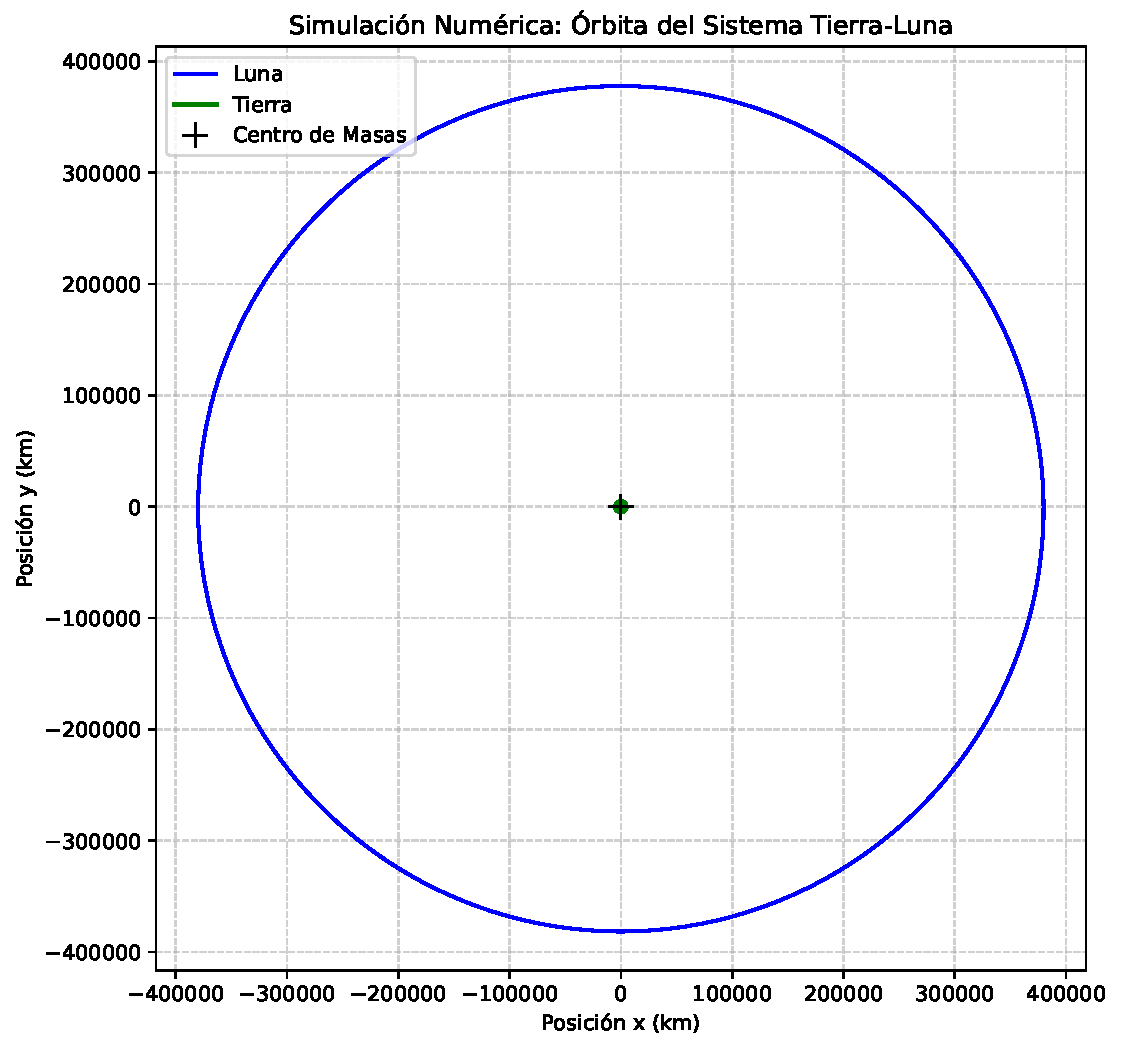
\includegraphics[width=0.7\linewidth]{lunarorbit}
    \caption{Órbita lunar calculada numéricamente con un período aproximado de 28 días}
    \label{fig:ÓrbitaLunar}
\end{figure}


\subsubsection*{Nota Computacional: La Importancia del Centro de Masas}

Es muy instructivo preguntarse: \textit{¿Qué habría pasado si, al programar la simulación, hubiéramos puesto a la Tierra inmóvil en el origen ($\boldsymbol{p}_T = \boldsymbol{0}$) y le hubiéramos dado toda la velocidad a la Luna?}

Físicamente, las Leyes de Newton seguirían siendo válidas. El problema sería de perspectiva. Al hacer esto, la cantidad de movimiento total del sistema dejaría de ser cero ($\boldsymbol{P}_{\text{total}} = m_L \boldsymbol{v}_L \neq \boldsymbol{0}$). Como la cantidad de movimiento se conserva, el Centro de Masas de nuestro sistema Tierra-Luna adquiriría una velocidad de traslación constante.

\textbf{Consecuencias en la simulación:}
\begin{itemize}
    \item \textbf{Visuales:} En lugar de dibujar elipses cerradas, el gráfico mostraría al sistema entero salir ``volando'' fuera de la pantalla. La trayectoria de la Luna parecería un resorte estirado (epicicloide), y la Tierra se tambalearía mientras es arrastrada por el espacio.
    \item \textbf{Analíticas:} Nuestro sencillo algoritmo para calcular el período (medir cuándo la Luna cruza el eje $x$) fallaría rotundamente, ya que el sistema entero se estaría desplazando por el eje $y$, alejándose del origen para siempre.
\end{itemize}

Al tomarnos el trabajo algebraico de inicializar los vectores $\boldsymbol{r}$ y $\boldsymbol{p}$ en el \textbf{Sistema del Centro de Masas} ($\boldsymbol{P}_{\text{total}} = \boldsymbol{0}$), eliminamos todo este caótico movimiento de traslación galileana. Este truco aísla la dinámica interna (la órbita pura) de la cinemática externa (el viaje por el espacio), demostrando que elegir un buen sistema de referencia es la mitad del trabajo en la resolución de cualquier problema físico.

\section{Momento angular}



A partir del vector de momento lineal se puede construir un nuevo vector de momento angular que mide la capacidad de un objeto para rotar. 

La magnitud del momento angular es la distancia desde un centro de giro al objeto, multiplicado por el momento lineal perpendicular a la dirección de centro de giro

% --- Inicio del código LaTeX para insertar ---

\begin{figure}[h!]
    \centering
    \begin{tikzpicture}[
        scale=1.5,
        font=\large,
        vector/.style={->, >=Stealth, ultra thick},
        helpline/.style={dashed, gray, thin}
    ]
        % --- Origen y Ejes de Referencia ---
        \node[label={below left:Origen (O)}] (O) at (0,0) {};
        \fill (O) circle (1.5pt);

        % --- Posición de la partícula y vector de posición ---
        \def\angleR{30} % Ángulo del vector de posición
        \def\magR{3.5}  % Magnitud del vector de posición
        \coordinate (P) at (\angleR:\magR); % Coordenada de la partícula
        
        \draw[vector, black] (O) -- (P) node[midway, above, sloped] {$\boldsymbol{r}$};
        \shade[ball color=blue] (P) circle (0.1cm) node[above right] {Partícula};

        % --- Vector de Momento Lineal ---
        \def\angleP{80} % Ángulo del vector de momento
        \def\magP{2.5}  % Magnitud del vector de momento
        \coordinate (PEnd) at ($(P) + (\angleP:\magP)$); % Coordenada del final del vector p
        
        % Dibujar el vector de momento total
        \draw[vector, red] (P) -- (PEnd) node[anchor=south west] {$\boldsymbol{p} = m\boldsymbol{v}$};
        
        % --- Descomposición del vector de momento p (Nuevo método) ---
        
        % 1. Calcular la longitud de la proyección de p sobre r
        \pgfmathsetmacro{\projLength}{\magP*cos(\angleP-\angleR)}
        
        % 2. Dibujar la componente Paralela (p_parallel)
        %    Un vector que parte de P, en la dirección de r, con la longitud de la proyección.
        \draw[vector, red!50] (P) -- ++(\angleR:\projLength) node[midway, below, sloped] {$\boldsymbol{p}_{\parallel}$};
        \coordinate (ParallelEnd) at ($(P) + (\angleR:\projLength)$);
        
        % 3. Dibujar la componente Perpendicular (p_perp)
        %    Un vector que parte de P, en la dirección perpendicular a r.
        \draw[vector, red!50, thick] (P) -- ++(\angleR+90:{\magP*sin(\angleP-\angleR)}) node[midway, above, sloped] {$\boldsymbol{p}_{\perp}$};
        
        % --- Dibujar el paralelogramo de suma de vectores ---
        \draw[helpline] (ParallelEnd) -- (PEnd);
        \draw[helpline] ($(P) + (\angleR+90:{\magP*sin(\angleP-\angleR)})$) -- (PEnd);
        
        % --- Marcar Ángulos ---
        % Ángulo theta entre r y p
        \draw[helpline] (P) -- ++(\angleR:3); % Extender línea de r
        \draw[->, gray] ($(P)+(\angleR:0.8)$) arc (\angleR:\angleP:0.8);
        \node at ({(\angleR+\angleP)/2}:1) [shift=(P)] {$\theta$};
        
    \end{tikzpicture}
    \caption{
        Ilustración mejorada de la definición de momento angular.
        El momento lineal $\boldsymbol{p}$ se descompone en una componente paralela a $\boldsymbol{r}$ ($\boldsymbol{p}_{\parallel}$) y una perpendicular ($\boldsymbol{p}_{\perp}$), ambas originadas en la partícula.
        El momento angular solo depende de la componente perpendicular: $\boldsymbol{L} = \boldsymbol{r} \times \boldsymbol{p}_{\perp}$.
        Su magnitud es $L = |\boldsymbol{r}| |\boldsymbol{p}_{\perp}| = r (p \sin\theta)$.
    }
    \label{fig:momento_angular_def_mejorada}
\end{figure}

% --- Fin del código LaTeX --



El momento angular se define como el producto vectorial (ver ecuación~\eqref{eq:crossproduct})
\begin{align}
\label{eq:L}
    \boldsymbol{L} = \boldsymbol{r}\times \boldsymbol{p}\,.
\end{align}
Ver figura~\ref{fig:momento_angular_def_mejorada}. La dirección viene dada por el producto vectorial entre los vectores de posición y momento lineal, que da como resultado un vector perpendicular al plano definido por los vectores de posición y momento lineal con su dirección determinada por la regla de la mano derecha.
%cómo se muestra en la figura \ref{fig:manoderecha}b.

La magnitud es
\begin{align}
    |\boldsymbol{L}| = |\boldsymbol{r}| |\boldsymbol{p}|\sin\theta\,,
\end{align}
donde $\theta$ es el ángulo formado por los vectores $\boldsymbol{r}$ y $\boldsymbol{p}$ en el plano $x-y$ como se ilustra en la figura~\ref{fig:momento_angular_3d_corregido}. donde se ilustra también la dirección del vector de momento angular $\boldsymbol{L}$ a lo largo de la dirección perpendicular $z$.

Podemos definir de igual forma el torque como
\begin{align}
    \boldsymbol{\tau} =  \boldsymbol{r}\times \boldsymbol{F}\,.
\end{align}


La inercia a la rotación es una característica de los objetos extendidos: en ausencia de torques externos un cuerpo mantiene el momento angular constante.

Un ejemplo es un pulsar que mantiene un período constante por largos períodos de tiempo. Sin embargo, con el paso del tiempo, va disminuyendo el período de rotación porqué pierde energía emitiendo ondas gravitacionales.



\subsection{Conservación del momento angular}
\subsubsection{Principio de Conservación del Momento Angular}

A partir de las definiciones vectoriales de momento angular ($\boldsymbol{L} = \boldsymbol{r} \times \boldsymbol{p}$) y torque ($\boldsymbol{\tau} = \boldsymbol{r} \times \boldsymbol{F}$), surge una de las leyes de conservación más importantes del universo:

\begin{quote}
    \textbf{Conservación del Momento Angular:} Si el torque externo neto que actúa sobre un sistema es cero ($\boldsymbol{\tau}_{\text{neto}} = \boldsymbol{0}$), el vector de momento angular total del sistema ($\boldsymbol{L}$) permanece constante en el tiempo.
\end{quote}

Esta conservación ocurre típicamente en dos escenarios fundamentales:
\begin{enumerate}
    \item \textbf{Sistemas Aislados:} Como un púlsar girando en el espacio profundo o una rueda de bicicleta girando libremente (inercia rotacional), donde simplemente no hay fuerzas externas aplicadas.
    \item \textbf{Fuerzas Centrales:} Como el caso de la gravedad. Aunque el Sol ejerce una fuerza inmensa sobre la Tierra, el vector de fuerza $\boldsymbol{F}_g$ es siempre paralelo al vector de posición $\boldsymbol{r}$ (apunta hacia adentro a lo largo de la misma línea). Por las propiedades del producto vectorial, el producto cruz de dos vectores paralelos es cero ($\boldsymbol{r} \times \boldsymbol{F}_g = \boldsymbol{0}$). Al no haber un torque que ``empuje de lado'', el momento angular de la órbita terrestre es una cantidad matemáticamente inviolable.
\end{enumerate}


El elevado momento angular de una rueda que gira a gran velocidad genera un gran efecto giroscópico. Al montar en bicicleta, esta resistencia a la variación del vector de momento angular ayuda a mantener la rueda en posición vertical y contribuye a la estabilidad. Ver figura~\ref{fig:rueda}

\begin{figure}
    \centering
    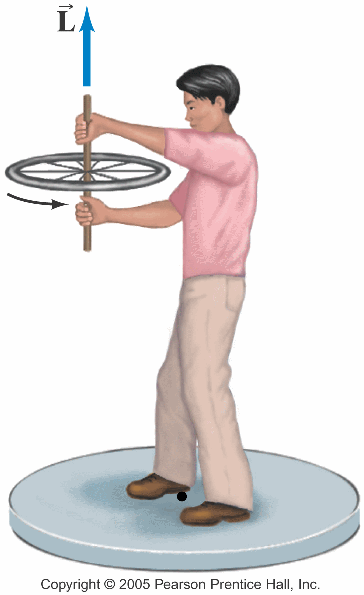
\includegraphics[scale = 0.3]{rueda}
    \caption{Vector de momento angular asociado al giro de una rueda de bicicleta}
    \label{fig:rueda}
\end{figure}
% --- Inicio del código LaTeX para insertar ---

% --- Inicio del código LaTeX para insertar ---

\begin{figure}[h!]
    \centering
    \begin{tikzpicture}[
        scale=2, % Escala para hacer la figura más grande
        font=\large,
        axis/.style={->, >=Stealth}, % Estilo para los ejes
        vector/.style={->, >=Stealth, ultra thick}, % Estilo para los vectores
        line/.style={dashed, thin} % Estilo para líneas de ayuda
    ]
        % --- Definir la perspectiva (proyección 3D en 2D) ---
        \def\perspX{-0.707}
        \def\perspY{-0.707}

        % --- Dibujar los ejes de coordenadas ---
        \draw[axis] (0,0) -- (2.*\perspX, 2.*\perspY) node[below] {$x$};
        \draw[axis] (0,0) -- (3,0) node[below] {$y$}; % Eje Y
        \draw[axis] (0,0) -- (0,2) node[left] {$z$};
        \node[anchor=north east] at (0.2,0) {O};
        
        % --- Posición de la partícula y vectores ---
        % Coordenadas de la partícula en el plano XY
        \coordinate (P) at (1, -0.5); % Posición de la partícula (m)

        % Dibujar la partícula 'm'
        \fill (P) circle (1.5pt) node[above left, xshift=12pt] {$m$};
        
        % Vector de posición r (azul)
        \draw[vector, blue] (0,0) -- (P) node[midway, below left] {$\boldsymbol{r}$};

        % Vector de momento P (verde)
        % Le damos un pequeño ángulo con respecto a la horizontal para que no sea paralelo al eje Y
        \def\angleP{5} % Ángulo del vector P con respecto a la horizontal
        \coordinate (PEnd) at ($(P) + (\angleP:1.5)$); % Coordenada del final de P
        \draw[vector, green!50!black] (P) -- (PEnd) node[midway, above] {$\boldsymbol{P}$};
        
        % --- Dibujar el vector Momento Angular L ---
        \draw[vector, red!70!black] (0,0) -- (0,1.5);
        \node at (0.6, 1.3) {$\boldsymbol{L} = \boldsymbol{r} \times \boldsymbol{P}$};
        
        % --- CORRECCIÓN: Detalles del ángulo phi ---
        % Extender la línea de acción del vector r
        \draw[line] (P) -- ($(P)!-1.5cm!(0,0)$);

        % Extender la línea de acción del vector P
        %\draw[line] (PEnd) -- ($(P)!-2.5cm!(PEnd)$);
        
        % Ángulo phi entre las dos líneas de acción
        % Calculamos el ángulo del vector r
        \pgfmathanglebetweenpoints{\pgfpointanchor{P}{center}}{\pgfpointorigin}
        \let\angleR\pgfmathresult
        
        % Dibujamos el arco desde el ángulo de P hasta el ángulo de r
        \draw[thick] ($(P) + (\angleP:1)$) arc (\angleP:\angleR-180:1);
        \node at ($(P) + ({(\angleP+\angleR-180)/2}:1.2)$) {$\theta$};

    \end{tikzpicture}
    \caption{Representación del vector de momento angular $\boldsymbol{L}$ como el producto vectorial del vector de posición $\boldsymbol{r}$ y el vector de momento lineal $\boldsymbol{P}$. El ángulo $\phi$ es el ángulo entre los dos vectores.}
    \label{fig:momento_angular_3d_corregido}
\end{figure}

% --- Fin del código LaTeX ---

\subsection{Demostración Algebraica de la Conservación del Momento Angular}

En la mecánica newtoniana, afirmamos que si el torque neto sobre un objeto es cero ($\boldsymbol{\tau} = \boldsymbol{0}$), su momento angular se conserva. A menudo, esto se demuestra usando reglas complejas de cálculo diferencial. Sin embargo, podemos demostrar la validez de este principio utilizando únicamente álgebra básica, la cinemática de pequeños incrementos ($\Delta t$) y las propiedades geométricas del producto vectorial.

\subsubsection{Paso 1: Definición del Cambio en el Momento Angular ($\Delta \boldsymbol{L}$)}

Partimos de la definición del vector de momento angular para una partícula de masa constante:
\begin{equation}
    \boldsymbol{L} = \boldsymbol{r} \times \boldsymbol{p}.
\end{equation}

Consideremos un intervalo de tiempo suficientemente pequeño $\Delta t$. Durante este intervalo, tanto la posición del objeto ($\boldsymbol{r}$) como su cantidad de movimiento ($\boldsymbol{p}$) pueden experimentar cambios, pasando a un estado final $\boldsymbol{r}_f = \boldsymbol{r} + \Delta\boldsymbol{r}$ y $\boldsymbol{p}_f = \boldsymbol{p} + \Delta\boldsymbol{p}$.

El momento angular final será:
\begin{equation}
    \boldsymbol{L}_f = \boldsymbol{r}_f \times \boldsymbol{p}_f = (\boldsymbol{r} + \Delta\boldsymbol{r}) \times (\boldsymbol{p} + \Delta\boldsymbol{p}).
\end{equation}

Usando la propiedad distributiva del producto cruz algebraico, expandimos esta expresión:
\begin{equation}
    \boldsymbol{L}_f = (\boldsymbol{r} \times \boldsymbol{p}) + (\boldsymbol{r} \times \Delta\boldsymbol{p}) + (\Delta\boldsymbol{r} \times \boldsymbol{p}) + (\Delta\boldsymbol{r} \times \Delta\boldsymbol{p}).
\end{equation}

El primer término ($\boldsymbol{r} \times \boldsymbol{p}$) es exactamente el momento angular inicial, $\boldsymbol{L}_i$. Si restamos $\boldsymbol{L}_i$ a ambos lados, obtenemos la ecuación algebraica para el cambio del momento angular ($\Delta \boldsymbol{L} = \boldsymbol{L}_f - \boldsymbol{L}_i$):
\begin{equation}
    \Delta \boldsymbol{L} = (\boldsymbol{r} \times \Delta\boldsymbol{p}) + (\Delta\boldsymbol{r} \times \boldsymbol{p}) + (\Delta\boldsymbol{r} \times \Delta\boldsymbol{p}).
    \label{eq:delta_L_algebraico}
\end{equation}

\subsubsection{Paso 2: Simplificación Cinemática (El término nulo)}

Analicemos el segundo término del lado derecho de nuestra ecuación: $(\Delta\boldsymbol{r} \times \boldsymbol{p})$.
Recordemos de la cinemática básica que el desplazamiento $\Delta\boldsymbol{r}$ ocurre en la misma dirección que la velocidad $\boldsymbol{v}$ a lo largo de un intervalo $\Delta t$ ($\Delta\boldsymbol{r} \approx \boldsymbol{v}\Delta t$). Y por definición, la cantidad de movimiento $\boldsymbol{p}$ es paralela a la velocidad ($\boldsymbol{p} = m\boldsymbol{v}$).

Por consiguiente, el desplazamiento y el momento son vectores paralelos. Una de las propiedades fundamentales del producto cruz establece que el producto vectorial de dos vectores paralelos es siempre cero (ya que $\sin(0^\circ) = 0$). Así que:
\begin{equation}
    \Delta\boldsymbol{r} \times \boldsymbol{p} = \boldsymbol{0}.
\end{equation}

Además, el último término $(\Delta\boldsymbol{r} \times \Delta\boldsymbol{p})$ es el producto de dos cantidades extremadamente pequeñas, por lo que su valor es despreciable en comparación con los demás términos de la ecuación. 

Al eliminar estos términos, nuestra ecuación de cambio se simplifica drásticamente a:
\begin{equation}
    \Delta \boldsymbol{L} \approx \boldsymbol{r} \times \Delta\boldsymbol{p}.
    \label{eq:delta_L_simplificado}
\end{equation}

\subsubsection{Paso 3: Conexión con el Torque y la Conservación}

Aquí es donde conectamos la geometría con la dinámica. La Segunda Ley de Newton establece que el cambio en la cantidad de movimiento es igual a la fuerza neta multiplicada por el tiempo de acción: $\Delta\boldsymbol{p} = \boldsymbol{F} \Delta t$.

Sustituimos esta equivalencia dinámica en la Ecuación (\ref{eq:delta_L_simplificado}):
\begin{equation}
    \Delta \boldsymbol{L} = \boldsymbol{r} \times (\boldsymbol{F} \Delta t).
\end{equation}

Como el tiempo $\Delta t$ es un número escalar, podemos factorizarlo algebraicamente fuera del producto cruz:
\begin{equation}
    \Delta \boldsymbol{L} = (\boldsymbol{r} \times \boldsymbol{F}) \Delta t.
\end{equation}

Reconocemos inmediatamente que el término entre paréntesis es la definición formal del torque: $\boldsymbol{\tau} = \boldsymbol{r} \times \boldsymbol{F}$. Por lo tanto:
\begin{equation}
    \Delta \boldsymbol{L} = \boldsymbol{\tau} \Delta t.
\end{equation}

\textbf{Conclusión Lógica:}
Si el torque neto aplicado sobre el objeto es igual a cero ($\boldsymbol{\tau} = \boldsymbol{0}$), entonces la ecuación nos obliga ineludiblemente a que:
\begin{equation}
    \Delta \boldsymbol{L} = \boldsymbol{0} \cdot \Delta t = \boldsymbol{0}.
\end{equation}
Al ser el cambio en el momento angular estrictamente nulo ($\Delta \boldsymbol{L} = \boldsymbol{0}$), queda demostrado algebraicamente que el vector $\boldsymbol{L}$ no cambia ni en magnitud ni en dirección; el momento angular \textbf{se conserva}.

\section{Derivación Simplificada de las Leyes de Kepler}

Derivar las leyes de Kepler para las orbita de los planetas del sistema solar, a partir de la Ley de Gravitación Universal de Newton, es uno de los triunfos históricos de la física. Aunque una derivación completa y rigurosa requiere el uso de cálculo diferencial, podemos entender la esencia de las tres leyes utilizando principalmente álgebra y conceptos de física a nivel introductorio.

\section*{Ley de Gravitación Universal de Newton (El Punto de Partida)}

Todo se basa en la ley de Newton, que dice que la fuerza de gravedad ($F_g$) entre dos objetos de masa $M$ y $m$ separados por una distancia $r$ es:
\[
    F_g = G \frac{Mm}{r^2}
\]
Donde $G$ es la constante de gravitación universal.

% --- Fin del código LaTeX ---

\section*{Primera Ley de Kepler (Ley de las Órbitas)}
\textbf{Enunciado:} \textit{“La órbita de cada planeta es una elipse con el Sol en uno de sus focos.”}

% --- Inicio del código LaTeX para insertar ---

\begin{figure}[h!]
    \centering
    \begin{tikzpicture}[
        scale=1.5,
        font=\large,
        dot/.style={fill, circle, inner sep=1.5pt}
    ]
        % --- Definir los parámetros de la elipse ---
        \def\a{4} % Semieje mayor
        \def\b{2.5} % Semieje menor
        % Calcular la distancia focal c, usando c^2 = a^2 - b^2
        \pgfmathsetmacro{\c}{sqrt(\a*\a - \b*\b)}

        % --- Dibujar la órbita elíptica ---
        \draw[blue, thick] (0,0) ellipse ({\a} and {\b});

        % --- Dibujar los ejes y semiejes ---
        % Eje mayor (línea horizontal)
        \draw[gray, dashed] (-\a, 0) -- (\a, 0);
        % Eje menor (línea vertical)
        \draw[gray, dashed] (0, -\b) -- (0, \b);
        
        % Marcar el centro
        \node[dot, label={below:Centro}] at (0,0) {};

        % --- Dibujar y etiquetar los focos ---
        \node[dot, label={below:$F_1$}] at (-\c, 0) {};
        % Colocar el Sol en el segundo foco (F2)
        \shade[ball color=yellow] (\c, 0) circle (0.3cm);
        \node[below, yshift=-12pt] at (\c, 0) {Sol ($F_2$)};

        % --- Etiquetar los semiejes ---
        % Semieje mayor 'a'
        \draw[<->, thick, red] (0,0) -- (\a, 0) node[midway, below] {$a$};
        
        % Semieje menor 'b'
        \draw[<->, thick, red] (0,0) -- (0, \b) node[midway, right] {$b$};
        
        % --- Mostrar un planeta en la órbita ---
        \def\anglePlanet{110} % Ángulo para la posición del planeta
        \coordinate (P) at ({\a*cos(\anglePlanet)}, {\b*sin(\anglePlanet)});
        \shade[ball color=brown!60] (P) circle (0.15cm);
        \node[above] at (P) {Planeta};
        
        % Línea que une el Sol y el planeta (para la 2da Ley de Kepler)
        \draw[gray] (\c, 0) -- (P);

    \end{tikzpicture}
    \caption{Ilustración de la Primera Ley de Kepler. La órbita del planeta es una elipse, con el Sol situado en uno de sus dos focos ($F_2$). Se muestran el semieje mayor ($a$) y el semieje menor ($b$).}
    \label{fig:orbita_eliptica}
\end{figure}

% --- Fin del código LaTeX ---

\paragraph{Derivación Simplificada:}
Una demostración rigurosa de que las órbitas son elipses requiere cálculo avanzado. Sin embargo, podemos demostrar que una \textbf{órbita circular} es un caso perfectamente válido y estable.
\begin{enumerate}
    \item \textbf{Condición para una Órbita Circular:} Para que un planeta se mueva en un círculo de radio $r$ a velocidad constante $v$, la fuerza de gravedad debe proporcionar exactamente la \textbf{fuerza centrípeta} necesaria, $F_c = \frac{mv^2}{r}$.

    \item \textbf{Igualando las Fuerzas:}
    \[ \text{Fuerza Gravitacional} = \text{Fuerza Centrípeta} \]
    \[ G \frac{M m}{r^2} = \frac{m v^2}{r} \]

    \item \textbf{Resolviendo para la Velocidad:} Simplificamos la ecuación cancelando una $m$ y una $r$ de cada lado:
    \[ G \frac{M}{r} = v^2 \implies v = \sqrt{\frac{GM}{r}} \]
\end{enumerate}
\paragraph{Conclusión (Simplificada):} Esta ecuación nos dice que para cualquier distancia $r$ del Sol, existe una velocidad específica $v$ que permite una órbita circular estable. Si un planeta tuviera una velocidad ligeramente diferente, su órbita se estiraría para convertirse en una \textbf{elipse}. El círculo es solo el caso especial de una elipse donde los dos focos coinciden.

\section*{Segunda Ley de Kepler (Ley de las Áreas)}
\textbf{Enunciado:} \textit{“Una línea que une un planeta y el Sol barre áreas iguales en intervalos de tiempo iguales.”}


\paragraph{Derivación Simplificada (usando Conservación del Momento Angular):}
Esta ley es una consecuencia directa de la \textbf{conservación del momento angular}.
\begin{enumerate}
    \item \textbf{Momento Angular ($L$):} El momento angular es una medida de la ``cantidad de movimiento de rotación'' y se calcula de acuerdo a la ecuación~\eqref{eq:L} como ($\boldsymbol{p} = m\boldsymbol{v}$)
    \begin{align*}
        \boldsymbol{L} = &\boldsymbol{r}\times\boldsymbol{p}\nonumber\\
        =& m \boldsymbol{r}\times\boldsymbol{v}\,,
    \end{align*}
    con magnitud
    \begin{align}
    \label{eq:Leqmvr}
     L =& m v r\sin\theta\nonumber\\
       =& m_{\perp} r
    \end{align}
    donde $v_{\perp}=v\sin\theta$ es la componente de la velocidad perpendicular a la línea que une el planeta con el Sol.

    \item \textbf{¿Por qué se Conserva?} La fuerza de gravedad es una \textbf{fuerza central}, siempre apunta hacia el Sol. No tiene ninguna componente ``de lado'' que pueda cambiar la rotación del planeta. Por lo tanto, el momento angular es constante:
    \[ L = m v_{\perp} r = \text{constante} \]

    \item \textbf{Conectando con el Área:} En un intervalo de tiempo muy corto $\Delta t$, el planeta se mueve una distancia. El área barrida ($\Delta A$) es aproximadamente un triángulo delgado con base $r$ y altura $v_{\perp} \Delta t$.
    \[ \Delta A \approx \frac{1}{2} (\text{base}) (\text{altura}) = \frac{1}{2} (r) (v_{\perp} \Delta t) \]

    \item \textbf{Tasa de Barrido de Área:} Dividiendo por $\Delta t$, obtenemos la ``velocidad'' a la que se barre el área:
    \[ \frac{\Delta A}{\Delta t} = \frac{1}{2} r v_{\perp} \]
    Usando la definición de momento angular $L = m v_{\perp} r$, podemos reescribir esto como:
    \[ \frac{\Delta A}{\Delta t} = \frac{L}{2m} \]
\end{enumerate}
\paragraph{Conclusión:} Como $L$, $m$ y 2 son constantes, la tasa de barrido de área ($\frac{\Delta A}{\Delta t}$) también debe ser \textbf{constante}. Esto significa que en intervalos de tiempo iguales, se barren áreas iguales, lo que demuestra la Segunda Ley. Esto explica por qué los planetas se mueven más rápido cuando están cerca del Sol y más lento cuando están lejos.

\section*{Tercera Ley de Kepler (Ley de los Períodos)}
\textbf{Enunciado:} \textit{“El cuadrado del período orbital de un planeta es directamente proporcional al cubo del semieje mayor de su órbita.”} Para órbitas circulares, esto se simplifica a ``El cuadrado del período es proporcional al cubo del radio".

\paragraph{Derivación Simplificada (para Órbitas Circulares):}
\begin{enumerate}
    \item \textbf{Período Orbital (T):} El período es el tiempo para completar una órbita. Para un círculo, la distancia es la circunferencia ($2\pi r$).
    \[ T = \frac{\text{Distancia}}{\text{Velocidad}} = \frac{2\pi r}{v} \]

    \item \textbf{Relacionando con la Gravedad:} De la Primera Ley, sabemos que la velocidad de una órbita circular es:
    \[ v = \sqrt{\frac{GM}{r}} \]

    \item \textbf{Sustituir la Velocidad:} Sustituimos esta expresión para $v$ en la ecuación del período.
    \[ T = \frac{2\pi r}{\sqrt{\frac{GM}{r}}} \]

    \item \textbf{Resolver para $T^2$:} Elevamos al cuadrado ambos lados para eliminar la raíz cuadrada.
    \[ T^2 = \frac{(2\pi r)^2}{\left(\sqrt{\frac{GM}{r}}\right)^2} = \frac{4\pi^2 r^2}{\frac{GM}{r}} \]

    \item \textbf{Simplificar la Fracción:}
    \[ T^2 = 4\pi^2 r^2 \cdot \frac{r}{GM} = \frac{4\pi^2 r^3}{GM} \]
\end{enumerate}
\paragraph{Conclusión:}
Podemos reescribir la ecuación como:
\[ T^2 = \left(\frac{4\pi^2}{GM}\right) r^3 \]
El término entre paréntesis es una constante para todos los objetos que orbitan la misma masa central $M$. Por lo tanto, hemos demostrado que:
\[ T^2 \propto r^3 \]
El cuadrado del período es directamente proporcional al cubo del radio, lo cual es la Tercera Ley de Kepler para órbitas circulares.

En general,% para un planeta de masa $m$ orbitando alrededor del sol con masa $M$
$$T^2 = \frac{4\pi^2}{G(M + m)} a^3$$

% --- Fin del código LaTeX ---

\section*{Ejemplo. Período orbital de la Luna}

The numerical value for the Moon's orbital period around the Earth can be precisely calculated using the generalized form of Kepler's third law, which accounts for the masses of both bodies.

\subsection*{The Formula}
The formula is given by:

$$T^2 = \frac{4\pi^2}{G(M_E + M_M)} a^3$$

Where $T$ is the orbital period and $a$ is the semi-major axis.

\subsection*{Calculation with Constants}
Using the constants defined in the previous section:

\begin{itemize}
    \item $G = \SI{6.674E-11}{\cubic\metre\per\kilogram\per\square\second}$
    \item $M_E + M_M \approx \SI{6.045E24}{\kilogram}$
    \item $a = \SI{3.844E8}{\metre}$
\end{itemize}

The calculation yields:

\begin{align*}
    T^2 &\approx \frac{4\pi^2}{(\SI{6.674E-11}{\meter^3\per\kilogram\per\second\squared})(\SI{6.045E24}{\kilogram})} (\SI{3.844E8}{\meter})^3 \\
    T^2 &\approx \SI{5.56E12}{\square\second} \\
    T &\approx \SI{2.358E6}{\second}
\end{align*}

\subsection*{Result}
The calculated orbital period is:

\begin{itemize}
    \item \textbf{In seconds:} $\approx \SI{2358000}{\second}$
    \item \textbf{In days:} $\approx \SI{27.3}{\day}$
\end{itemize}

This theoretical value matches the observed sidereal period of the Moon.

\section{Ejemplos de las Leyes de Newton}

% --- Inicio del código LaTeX para insertar ---

\section*{Ejemplo: Problema de Trabajo y Energía en una Rampa}

\paragraph{Enunciado del Problema:}
En la bolera, el mecanismo alimentador de bolas debe ejercer una fuerza para empujar las bolas de boliche por una rampa de \SI{1.0}{\meter} de largo. La rampa lleva las bolas a un conducto \SI{0.5}{\meter} por encima de la base de la rampa. ¿Aproximadamente cuánta fuerza debe ejercerse sobre una bola de boliche de \SI{5.0}{\kilo\gram}?

\begin{enumerate}[label=(\alph*)]
    \item \SI{200}{\newton}
    \item \SI{50}{\newton}
    \item \SI{25}{\newton}
    \item \SI{5.0}{\newton}
    \item imposible de determinar
\end{enumerate}

\subsection*{Solución Detallada}

La respuesta correcta es \textbf{(c) \SI{25}{\newton}}. Este problema se puede resolver de dos maneras principales: utilizando el Teorema del Trabajo y la Energía o analizando las fuerzas en un plano inclinado.

\paragraph{Método 1: Usando el Teorema del Trabajo y la Energía (el más directo)}
El Teorema del Trabajo y la Energía establece que el trabajo realizado sobre un objeto se convierte en su cambio de energía. En este caso, el trabajo realizado por el mecanismo ($W$) se convierte en la energía potencial gravitacional ($\Delta U_g$) de la bola al ganar altura. Asumimos que la bola se mueve a velocidad constante, por lo que no hay cambio en su energía cinética.

\begin{itemize}
    \item Trabajo realizado: $W = F \cdot d$, donde $F$ es la fuerza aplicada y $d$ es la distancia a lo largo de la rampa.
    \item Cambio de Energía Potencial: $\Delta U_g = mgh$, donde $m$ es la masa, $g$ la gravedad y $h$ la altura vertical.
\end{itemize}
\textbf{Datos del problema:}
\begin{itemize}
    \item Distancia a lo largo de la rampa, $d = \SI{1.0}{\meter}$.
    \item Masa de la bola, $m = \SI{5.0}{\kilo\gram}$.
    \item Altura vertical, $h = \SI{0.5}{\meter}$.
    \item Aceleración de la gravedad, $g \approx \SI{9.8}{\meter\per\second\squared}$.
\end{itemize}
\textbf{Cálculo:}
Igualamos el trabajo y el cambio de energía potencial:
\[ W = \Delta U_g \implies F \cdot d = mgh \]
Despejamos la fuerza $F$:
\[ F = \frac{mgh}{d} \]
Sustituimos los valores:
\[ F = \frac{(\SI{5.0}{\kilo\gram}) \times (\SI{9.8}{\meter\per\second\squared}) \times (\SI{0.5}{\meter})}{\SI{1.0}{\meter}} = \frac{\SI{24.5}{\joule}}{\SI{1.0}{\meter}} = \SI{24.5}{\newton} \]
El valor calculado es de \SI{24.5}{\newton}, que se aproxima a la opción \textbf{\SI{25}{\newton}}.

\paragraph{Método 2: Usando Fuerzas en un Plano Inclinado}
Este método consiste en encontrar la componente de la fuerza de gravedad que actúa a lo largo de la rampa y que el mecanismo debe contrarrestar.

\begin{enumerate}
    \item \textbf{Encontrar el ángulo de la rampa ($\theta$):}
    La rampa forma un triángulo rectángulo con hipotenusa $d=\SI{1.0}{\meter}$ y cateto opuesto $h=\SI{0.5}{\meter}$.
    \[ \sin(\theta) = \frac{\text{opuesto}}{\text{hipotenusa}} = \frac{\SI{0.5}{\meter}}{\SI{1.0}{\meter}} = 0.5 \]
    Esto corresponde a un ángulo de $\theta = \ang{30}$.

    \item \textbf{Calcular la componente del peso a lo largo de la rampa ($F_{g, \parallel}$):}
    La fuerza de la gravedad que tira de la bola hacia abajo a lo largo de la rampa es la componente del peso paralela al plano.
    \[ F_{g, \parallel} = mg \sin(\theta) \]
    
    \item \textbf{Sustituir los valores:}
    \[ F_{g, \parallel} = (\SI{5.0}{\kilo\gram}) \times (\SI{9.8}{\meter\per\second\squared}) \times \sin(\ang{30}) \]
    \[ F_{g, \parallel} = (\SI{49}{\newton}) \times 0.5 = \SI{24.5}{\newton} \]
\end{enumerate}
Para empujar la bola hacia arriba a velocidad constante, la fuerza aplicada por el mecanismo debe ser igual en magnitud a esta componente del peso. Por lo tanto, la fuerza requerida es de \SI{24.5}{\newton}. Ambos métodos confirman que la respuesta correcta es \textbf{\SI{25}{\newton}}.

% --- Fin del código LaTeX ---
\section{Ejercicios}

\subsection{Ejercicio Conceptual: Tiempos de Vuelo en Lanzamiento Vertical}

\textbf{Enunciado del Problema:} Un barco de guerra dispara simultáneamente dos proyectiles de forma exactamente vertical hacia arriba. Si los proyectiles alcanzan las alturas máximas mostradas en la figura (despreciando la resistencia del aire), ¿qué proyectil regresa primero al nivel del barco?

\begin{center}
\begin{tikzpicture}[scale=1.2, >=stealth]
    % Superficie del agua
    \fill[cyan!10] (-3.5, -0.4) rectangle (3.5, 0);
    \draw[thick, cyan!50!black] (-3.5, 0) -- (3.5, 0);

    % Barco principal (Acorazado)
    \draw[thick, fill=gray!30] (-2.5,0) -- (-2.8, 0.5) -- (2.8, 0.5) -- (2.5, 0) -- cycle;
    \draw[thick, fill=gray!50] (-1.5, 0.5) rectangle (1.5, 1.0);
    \draw[thick, fill=gray!70] (-0.5, 1.0) rectangle (0.5, 1.5);
    \node[above, font=\bfseries] at (0, 1.5) {Acorazado};

    % Cañón y Proyectil A (Izquierda - Alto)
    \draw[thick, fill=black] (-1.8, 0.5) rectangle (-1.6, 0.8);
    % Trayectoria subida A
    \draw[dashed, thick, black, ->] (-1.7, 0.8) -- (-1.7, 4.0) node[above, font=\bfseries\large] {A};
    % Trayectoria bajada A (ligeramente desplazada para claridad visual)
    \draw[dashed, thick, gray, <-] (-1.5, 0.8) -- (-1.5, 4.0);

    % Cañón y Proyectil B (Derecha - Bajo)
    \draw[thick, fill=black] (1.6, 0.5) rectangle (1.8, 0.8);
    % Trayectoria subida B
    \draw[dashed, thick, black, ->] (1.7, 0.8) -- (1.7, 2.0) node[above, font=\bfseries\large] {B};
    % Trayectoria bajada B (ligeramente desplazada para claridad visual)
    \draw[dashed, thick, gray, <-] (1.9, 0.8) -- (1.9, 2.0);

\end{tikzpicture}
\end{center}

\begin{enumerate}
    \item El proyectil A
    \item Ambos al mismo tiempo
    \item El proyectil B
    \item Se necesita más información
\end{enumerate}

\subsubsection*{Solución Detallada}

La respuesta correcta es \textbf{(3) El proyectil B}. 

Este problema es la reducción a una dimensión (caída libre vertical) del concepto de tiempo de vuelo. Demuestra que el tiempo que un objeto pasa en el aire está dictado única y exclusivamente por la altura máxima que alcanza, independientemente de su masa (al despreciar la resistencia del aire).

\textbf{1. Relación entre la altura máxima y la velocidad inicial:}
De acuerdo con la ecuación cinemática sin tiempo ($v_f^2 = v_0^2 - 2g\Delta y$), en la altura máxima $H$ la velocidad final es cero. Despejando, obtenemos la relación entre la altura máxima y la velocidad inicial:
\begin{equation}
    H = \frac{v_{0}^2}{2g}.
\end{equation}
Al observar el diagrama, es evidente que el proyectil A alcanza una altura máxima mucho mayor que el proyectil B ($H_A > H_B$). Esto implica necesariamente que el proyectil A fue disparado con una velocidad inicial mayor ($v_{0, A} > v_{0, B}$).

\textbf{2. Relación entre la velocidad inicial y el tiempo de vuelo:}
Para un lanzamiento vertical que regresa a su punto de partida, el tiempo total de vuelo ($t_{\text{vuelo}}$) está determinado por la velocidad inicial y la aceleración de la gravedad:
\begin{equation}
    t_{\text{vuelo}} = \frac{2v_{0}}{g}.
\end{equation}

\textbf{Conclusión:}
Podemos relacionar el tiempo de vuelo directamente con la altura máxima. Despejando $v_0 = \sqrt{2gH}$ de la primera ecuación y sustituyéndolo en la segunda, obtenemos:
\begin{equation}
    t_{\text{vuelo}} = \frac{2\sqrt{2gH}}{g} = \sqrt{\frac{8H}{g}}.
\end{equation}
Por lo tanto,
\begin{equation}
    t_{\text{vuelo}} \propto \sqrt{H}.
\end{equation}
Esta proporcionalidad demuestra algebraicamente que \textbf{a mayor altura máxima, mayor es el tiempo de vuelo}. Dado que el proyectil A sube mucho más alto, pasa más tiempo desacelerando en la subida y acelerando en la bajada. Por el contrario, el proyectil B alcanza una altura menor, completando su ciclo de subida y bajada mucho más rápido. En consecuencia, el \textbf{proyectil B} impactará primero de regreso sobre la cubierta del barco.

\subsection*{Ejercicio Conceptual: Tiempos de Vuelo en el Movimiento Parabólico}

\textbf{Enunciado del Problema:} Un barco de guerra dispara simultáneamente dos proyectiles a barcos enemigos. Si los proyectiles siguen las trayectorias parabólicas mostradas en la figura (despreciando la resistencia del aire), ¿qué barco es alcanzado primero?

\begin{center}
\begin{tikzpicture}[scale=1.2, >=stealth]
    % Superficie del agua
    \fill[cyan!10] (-2.5, -0.4) rectangle (10.5, 0);
    \draw[thick, cyan!50!black] (-2.5, 0) -- (10.5, 0);

    % Barco principal (Acorazado)
    \draw[thick, fill=gray!30] (-2,0) -- (-2.2, 0.4) -- (-0.3, 0.4) -- (-0.1, 0) -- cycle;
    \draw[thick, fill=gray!50] (-1.7, 0.4) rectangle (-0.7, 0.8);
    \draw[thick, fill=gray!70] (-1.5, 0.8) rectangle (-1.3, 1.2);
    \draw[thick, fill=gray!70] (-1.0, 0.8) rectangle (-0.8, 1.1);
    \node[above, font=\bfseries] at (-1.2, 1.2) {Acorazado};

    % Cañón
    \draw[thick, fill=black] (-0.3, 0.1) -- (0.1, 0.2) -- (0.1, 0.05) -- cycle;

    % Barco A

    \draw[thick, fill=red!20] (3.7, 0) -- (3.6, 0.2) -- (4.4, 0.2) -- (4.3, 0) -- cycle;
    \draw[thick, fill=red!40] (3.9, 0.2) rectangle (4.1, 0.4);
    \node[above, font=\bfseries\large] at (4, 0.4) {A};

    % Barco B
    \draw[thick, fill=red!20] (9.7, 0) -- (9.6, 0.2) -- (10.4, 0.2) -- (10.3, 0) -- cycle;
    \draw[thick, fill=red!40] (9.9, 0.2) rectangle (10.1, 0.4);
    \node[above, font=\bfseries\large] at (10, 0.4) {B};

    % Trayectoria A (alta, corta)
    % Parábola: y = a*x*(x - 4) con vértice en (2, 3.5) -> 3.5 = a*2*(-2) -> a = -3.5/4 = -0.875
    \draw[dashed, thick, black, ->] plot[domain=0.1:4, samples=50] (\x, {-0.875*\x*(\x - 4)});

    % Trayectoria B (baja, larga)
    % Parábola: y = b*x*(x - 10) con vértice en (5, 1.5) -> 1.5 = b*5*(-5) -> b = -1.5/25 = -0.06
    \draw[dashed, thick, black, ->] plot[domain=0.1:10, samples=50] (\x, {-0.06*\x*(\x - 10)});

\end{tikzpicture}
\end{center}

\begin{enumerate}
    \item El barco A
    \item Ambos al mismo tiempo
    \item El barco B
    \item Se necesita más información
\end{enumerate}

\subsubsection*{Solución Detallada}

La respuesta correcta es \textbf{(3) El barco B}. 

Aunque la intuición inicial podría sugerir que el barco más cercano (A) es alcanzado primero, o que el proyectil que viaja más lejos (B) debe tardar más, la física del movimiento parabólico demuestra lo contrario. El tiempo de vuelo de un proyectil depende \textbf{exclusivamente de su movimiento vertical}.

\textbf{1. Relación entre la altura máxima y la velocidad inicial vertical:}
Como vimos en la sección de la Altura Máxima (Ecuación 3.48), la altura máxima $H$ alcanzada por un proyectil está dada por:
\begin{equation}
    H = \frac{v_{y0}^2}{2g}.
\end{equation}
Al observar el diagrama, es evidente que la trayectoria del proyectil hacia el barco A alcanza una altura máxima mucho mayor que la del proyectil hacia el barco B ($H_A > H_B$). Esto implica necesariamente que el proyectil A fue disparado con una componente de velocidad vertical inicial mucho mayor ($v_{y0, A} > v_{y0, B}$).

\textbf{2. Relación entre la velocidad inicial vertical y el tiempo de vuelo:}
En el ejemplo del tiempo de vuelo, demostramos que el tiempo total que un proyectil permanece en el aire ($t_{\text{vuelo}}$) está determinado únicamente por su velocidad vertical inicial y la gravedad:
\begin{equation}
    t_{\text{vuelo}} = \frac{2v_{y0}}{g}.
\end{equation}

\textbf{Conclusión:}
Al sustituir $v_{y0} = \sqrt{2gH}$ en la ecuación del tiempo de vuelo, obtenemos:
\begin{equation}
    t_{\text{vuelo}} \propto \sqrt{H}.
\end{equation}
Esto demuestra algebraicamente que \textbf{a mayor altura máxima, mayor es el tiempo de vuelo}. Dado que el proyectil dirigido al barco A sube mucho más alto, pasa mucho más tiempo en el aire "subiendo y bajando" que el proyectil rasante dirigido al barco B. Por lo tanto, el proyectil con la trayectoria más plana impactará primero, alcanzando al \textbf{barco B} antes de que el otro proyectil caiga sobre el barco A.

\subsection{Ejercicio Avanzado: La ``Caída'' de la Tierra}

\textbf{Enunciado del Problema:} 
Suponga que deja caer una piedra de masa $m = 1.0 \text{ kg}$ desde una altura $h = 100 \text{ m}$ sobre la superficie terrestre, partiendo del reposo. El sentido común y la experiencia cotidiana nos dicen que la piedra cae hacia la Tierra. Sin embargo, la Tercera Ley de Newton afirma que la piedra atrae a la Tierra con una fuerza exactamente de la misma magnitud con la que la Tierra atrae a la piedra.

Asumiendo que la Tierra está aislada en el espacio para este análisis:
\begin{enumerate}
    \item[a)] Calcule la magnitud de la aceleración con la que la Tierra ``cae'' hacia la piedra.
    \item[b)] Calcule la distancia total que se desplaza la Tierra hacia la piedra durante el tiempo de vuelo de la misma.
\end{enumerate}

\textbf{Datos necesarios:}
\begin{itemize}
    \item Masa de la piedra, $m = 1.0 \text{ kg}$.
    \item Aceleración de la gravedad, $g \approx 9.8 \text{ m/s}^2$.
    \item Masa de la Tierra, $M_T \approx 5.97 \times 10^{24} \text{ kg}$.
\end{itemize}

\subsubsection*{Solución Detallada}

\textbf{a) Cálculo de la Aceleración de la Tierra}

Según la \textbf{Ley de Gravitación Universal}, la fuerza con la que la Tierra atrae a la piedra es su propio peso:
\begin{equation}
    |\boldsymbol{F}_{\text{piedra}}| = mg = (1.0 \text{ kg})(9.8 \text{ m/s}^2) = 9.8 \text{ N}.
\end{equation}

Por la \textbf{Tercera Ley de Newton} (Acción y Reacción), la fuerza con la que la piedra atrae a la Tierra ($\boldsymbol{F}_T$) tiene exactamente la misma magnitud, pero dirección opuesta:
\begin{equation}
    |\boldsymbol{F}_T| = 9.8 \text{ N}.
\end{equation}

Para encontrar la aceleración de la Tierra ($a_T$), aplicamos la \textbf{Segunda Ley de Newton} al planeta entero ($|\boldsymbol{F}_T| = M_T a_T$):
\begin{equation}
    a_T = \frac{|\boldsymbol{F}_T|}{M_T} = \frac{9.8 \text{ N}}{5.97 \times 10^{24} \text{ kg}}.
\end{equation}

Al realizar el cálculo numérico, obtenemos:
\begin{equation}
    a_T \approx 1.64 \times 10^{-24} \text{ m/s}^2.
\end{equation}
\textbf{Respuesta a):} La Tierra se acelera hacia la piedra a unos insignificantes $1.64 \times 10^{-24} \text{ m/s}^2$.

\vspace{0.5cm}

\textbf{b) Cálculo de la Distancia Desplazada por la Tierra}

Podemos resolver esta parte de dos maneras diferentes que demuestran la consistencia de las leyes que hemos estudiado: usando cinemática o usando la conservación del Centro de Masas.

\textbf{Método 1: Usando Cinemática Básica}
Primero, calculamos el tiempo ($t$) que tarda la piedra en caer $100 \text{ m}$. Usamos la ecuación de posición para un objeto que parte del reposo ($v_{0} = 0$):
\begin{equation}
    h = \frac{1}{2} g t^2 \implies t = \sqrt{\frac{2h}{g}} = \sqrt{\frac{2(100 \text{ m})}{9.8 \text{ m/s}^2}} \approx 4.518 \text{ s}.
\end{equation}

Durante esos mismos $4.518 \text{ s}$, la Tierra se ha estado acelerando hacia arriba partiendo del reposo. Su desplazamiento ($d_T$) será:
\begin{equation}
    d_T = \frac{1}{2} a_T t^2 = \frac{1}{2} (1.64 \times 10^{-24} \text{ m/s}^2) (4.518 \text{ s})^2.
\end{equation}
\begin{equation}
    d_T \approx 1.67 \times 10^{-23} \text{ m}.
\end{equation}

\textbf{Método 2: Usando el Centro de Masas (Más elegante)}
\subsubsection{Conexión Conceptual: Posiciones vs. Desplazamientos del Centro de Masas}

El resultado algebraico que acabamos de utilizar para la caída de la Tierra ($M_T d_T = m h$) guarda una profunda e innegable similitud con la fórmula que derivamos anteriormente para los radios orbitales de un sistema binario ($m_1 r_1 = m_2 r_2$). Esta similitud no es una coincidencia, sino la manifestación de un mismo principio físico aplicado a dos dimensiones diferentes del movimiento: la posición estática y el desplazamiento cinemático.

A continuación, demostraremos algebraicamente por qué ambas fórmulas son dos caras de la misma moneda.

\textbf{1. El Enfoque Estático (Sistema Binario):} 

En el caso del sistema binario, ubicamos el origen de nuestro sistema de coordenadas exactamente en el Centro de Masas ($\boldsymbol{r}_{\text{CM}} = \boldsymbol{0}$). 
Utilizando la definición de la posición del Centro de Masas para dos partículas, tenemos
\begin{equation}
    \boldsymbol{0} = \frac{m_1\boldsymbol{r}_1 + m_2\boldsymbol{r}_2}{m_1 + m_2}.
\end{equation}
Al multiplicar por el denominador, obtenemos $\boldsymbol{0} = m_1\boldsymbol{r}_1 + m_2\boldsymbol{r}_2$, lo que implica que $m_1\boldsymbol{r}_1 = -m_2\boldsymbol{r}_2$. Tomando únicamente las magnitudes (las distancias absolutas al centro, $r_1$ y $r_2$), recuperamos nuestra ecuación geométrica:
\begin{equation}
    m_1 r_1 = m_2 r_2.
\end{equation}
Esta fórmula nos habla de \textbf{distancias estáticas}. Nos dice cómo debe distribuirse la masa alrededor del centro de equilibrio.

\textbf{2. El Enfoque Cinemático (La Caída de la Tierra):}

En el problema de la piedra y la Tierra, el sistema también está aislado, por lo que su Centro de Masas no puede moverse. Esto significa que el \textbf{desplazamiento} del Centro de Masas es cero ($\Delta\boldsymbol{r}_{\text{CM}} = \boldsymbol{0}$). 
Si utilizamos la ecuación de los desplazamientos que derivamos en la Ecuación (\ref{eq:desplazamiento_cm}):
\begin{equation}
    \boldsymbol{0} = \frac{M_T \Delta\boldsymbol{r}_T + m \Delta\boldsymbol{r}_{\text{piedra}}}{M_T + m}.
\end{equation}
De nuevo, el denominador desaparece al multiplicar por cero, dejándonos con
\begin{equation}
    M_T \Delta\boldsymbol{r}_T = - m \Delta\boldsymbol{r}_{\text{piedra}}.
\end{equation}
El signo negativo nos indica que si la piedra se desplaza hacia abajo, la Tierra debe desplazarse hacia arriba. Si tomamos las magnitudes de estos desplazamientos (llamando $d_T$ al desplazamiento de la Tierra y asumiendo que el desplazamiento de la piedra es aproximadamente su altura de caída, $|\Delta\boldsymbol{r}_{\text{piedra}}| \approx h$), obtenemos exactamente la fórmula que usamos para resolver el ejercicio:
\begin{equation}
    M_T d_T = m h.
\end{equation}

\textbf{Conclusión Matemática:}
La ecuación $m_1 r_1 = m_2 r_2$ nos garantiza que el Centro de Masas se mantiene en el \textbf{origen geométrico}, mientras que la ecuación $M_T d_T = m h$ nos garantiza que el Centro de Masas se mantiene en \textbf{reposo cinemático}. Ambas son la traducción algebraica directa del principio de conservación de la cantidad de movimiento aplicado a las distancias.


Sabiendo que el sistema Tierra-Piedra es un sistema aislado (la fuerza neta externa es cero), la posición de su Centro de Masas no puede cambiar. Por lo tanto, el desplazamiento de la masa de la Tierra compensa exactamente el desplazamiento de la masa de la piedra:
\begin{equation}
    M_T d_T = m h \implies d_T = h \left( \frac{m}{M_T} \right).
\end{equation}
Sustituyendo los valores:
\begin{equation}
    d_T = 100 \text{ m} \left( \frac{1.0 \text{ kg}}{5.97 \times 10^{24} \text{ kg}} \right) \approx 1.67 \times 10^{-23} \text{ m}.
\end{equation}

\textbf{Respuesta b):} La Tierra se mueve hacia la piedra una distancia aproximada de $1.67 \times 10^{-23} \text{ m}$.

\textbf{Interpretación Física:}
Para poner este asombroso resultado en perspectiva, el radio de un solo núcleo atómico es del orden de $10^{-15} \text{ m}$. El desplazamiento de la Tierra al caer la piedra es \textbf{cien millones de veces más pequeño que un núcleo atómico}. Por esta razón, en la física aplicada y en la vida cotidiana, es una aproximación matemáticamente perfecta asumir que la Tierra permanece rígidamente inmóvil mientras los objetos caen.

\subsubsection{Ejercicio Conceptual: La Paradoja de la Caída Libre (El Experimento Mental de Galileo).}
    
    Antes de los estudios de Galileo y Newton, la física aristotélica afirmaba que los objetos más pesados caían más rápido que los objetos más ligeros. Para demostrar que esta suposición era ilógica, Galileo imaginó el escenario ilustrado en la Figura \ref{fig:paradoja_galileo}.
    
    Imagine dos piedras: una piedra pesada (Masa $M$) y una piedra ligera (Masa $m$). Según la teoría antigua, $M$ cae más rápido que $m$. Ahora imagine que atamos o pegamos ambas piedras con una cuerda para formar un solo objeto de masa combinada ($M + m$).
    
    \begin{figure}[htbp]
    \centering
    \begin{tikzpicture}[>=stealth, scale=1.1]
        
        % Línea de inicio (Techo / Reposo)
        \draw[thick, gray!80!black, dashed] (-1, 4) -- (8, 4);
        \node[above, gray!80!black] at (3.5, 4) {Línea de lanzamiento (Reposo)};

        % ESCENARIO 1: Piedra pesada (M)
        \coordinate (M) at (1, 2.5);
        \draw[fill=gray!60, thick] (M) circle (0.6) node[font=\large] {$M$};
        \draw[->, ultra thick, red] (1, 1.8) -- (1, -0.5) node[midway, left] {Rápido};

        % ESCENARIO 2: Piedra ligera (m)
        \coordinate (m) at (3.5, 3.2);
        \draw[fill=gray!30, thick] (m) circle (0.3) node {$m$};
        \draw[->, thick, blue] (3.5, 2.8) -- (3.5, 1.2) node[midway, left] {Lento};

        % ESCENARIO 3: Sistema Atado (M + m)
        \coordinate (M_tied) at (6.5, 2.2);
        \coordinate (m_tied) at (6.5, 3.3);
        
        % Cuerda tensa uniendo las masas
        \draw[thick, double, brown!80!black] (M_tied) -- (m_tied);
        
        % Piedras atadas
        \draw[fill=gray!60, thick] (M_tied) circle (0.6) node[font=\large] {$M$};
        \draw[fill=gray!30, thick] (m_tied) circle (0.3) node {$m$};

        % Contradicción (Flechas interrogativas punteadas)
        % Opción A (más lento por el freno de m)
        \draw[->, thick, purple, dashed] (5.7, 1.5) -- (5.7, 0.2) node[below, align=center, font=\footnotesize] {¿Frenado?\\($m$ retrasa a $M$)};
        % Opción B (más rápido por ser más pesado)
        \draw[->, ultra thick, orange!90!black, dashed] (7.3, 1.5) -- (7.3, -1.0) node[below, align=center, font=\footnotesize] {¿Acelerado?\\($M+m > M$)};

    \end{tikzpicture}
    \caption{El experimento mental de Galileo. Si los objetos pesados cayeran más rápido que los ligeros, atar dos piedras crearía un sistema que debería caer más lento (porque la piedra ligera lo frena) y, simultáneamente, más rápido (porque la masa total es mayor). Esta contradicción lógica solo se resuelve si la aceleración de caída es independiente de la masa.}
    \label{fig:paradoja_galileo}
    \end{figure}

    \begin{enumerate}
        \item[a)] Por un lado, argumente qué debería pasar con la velocidad de caída de este nuevo sistema si la piedra ligera, que se supone cae más despacio, actúa como un ``paracaídas'' o freno mecánico para la piedra pesada que intenta caer más rápido.
        \item[b)] Por otro lado, analice la masa total del nuevo objeto ($M + m$). Como esta masa combinada es mayor que la de la piedra pesada sola ($M+m > M$), argumente qué debería pasar con su velocidad de caída según la propia teoría antigua.
        \item[c)] Demuestre cómo estas dos conclusiones simultáneas generan una contradicción lógica insalvable. Finalmente, apoyándose en la ecuación de la Ley de Gravitación Universal y la Segunda Ley de Newton ($|\boldsymbol{F}| = ma$), explique algebraicamente cuál es la única resolución posible a esta paradoja en el mundo real. 
        
        \textit{[Resp. Conceptual: a) El sistema caería a una velocidad intermedia; b) El sistema caería más rápido que $M$ sola; c) La contradicción es que la misma configuración atada no puede caer simultáneamente más lento y más rápido que $M$. La única solución congruente, respaldada algebraicamente al igualar la gravedad y la inercia $\left(G\frac{M_T m}{r^2} = ma\right)$, es que la masa $m$ se cancela a ambos lados. La aceleración $a$ (que es la magnitud del campo gravitacional siempre presente) es estrictamente independiente de la masa, por ende, todos los objetos caen exactamente con la misma aceleración en el vacío]\footnote{Para una discusión al respecto se recomienda el podcast \url{ https://go.ivoox.com/rf/108254052} del minuto 20 al 50}.}
    \end{enumerate}


\subsubsection{Problemas Cuantitativos Propuestos}

A continuación, se presentan diez ejercicios para evaluar la asimilación de los conceptos dinámicos, energéticos y cinemáticos desarrollados en este capítulo. Se recomienda dibujar un diagrama de cuerpo libre o un esquema de la situación antes de plantear las ecuaciones. Use $g \approx 9.8 \text{ m/s}^2$ a menos que se indique lo contrario.

\begin{enumerate}
    \item \textbf{Leyes de Newton y Trabajo:} Un automóvil de masa $m = 1200 \text{ kg}$ acelera en línea recta desde el reposo hasta alcanzar una velocidad de $25 \text{ m/s}$ en un tiempo de $10 \text{ s}$ bajo la acción de una fuerza neta constante. 
    \begin{enumerate}
        \item Calcule la magnitud de la aceleración constante y la fuerza neta $\boldsymbol{F}$ aplicada sobre el vehículo.
        \item Utilizando la ecuación cinemática sin tiempo, calcule el desplazamiento total y luego encuentre el trabajo mecánico total $W$ realizado sobre el auto. \textit{[Resp: a) $a = 2.5 \text{ m/s}^2$, $F = 3000 \text{ N}$; b) $\Delta x = 125 \text{ m}$, $W = 375 \text{ kJ}$]}
    \end{enumerate}

    \item \textbf{Conservación de la Energía Mecánica:} Un bloque de piedra de $2.0 \text{ kg}$ se deja caer desde el reposo desde lo alto de un acantilado de $50 \text{ m}$ de altura. Despreciando la resistencia del aire y utilizando exclusivamente el principio de conservación de la energía mecánica ($K_i + U_i = K_f + U_f$), calcule la magnitud de la velocidad del bloque justo un instante antes de impactar contra el suelo. \textit{[Resp: $v_f \approx 31.3 \text{ m/s}$]}

    \item \textbf{Movimiento Parabólico:} Un jugador de fútbol patea un balón desde el nivel del suelo, imprimiéndole una velocidad inicial de $20 \text{ m/s}$ con un ángulo de elevación de $45^\circ$ respecto a la horizontal. 
    \begin{enumerate}
        \item Calcule la altura máxima $H$ alcanzada por el balón.
        \item Calcule el alcance horizontal máximo $R$. \textit{[Resp: a) $H \approx 10.2 \text{ m}$; b) $R \approx 40.8 \text{ m}$]}
    \end{enumerate}

    \item \textbf{Fuerzas y Fricción con Ángulo:} Un cajón de madera de $10 \text{ kg}$ es arrastrado hacia la derecha sobre un piso horizontal. Una persona tira de él mediante una cuerda que ejerce una fuerza de $50 \text{ N}$ formando un ángulo de $30^\circ$ por encima de la horizontal. Si el cajón se mueve con \textbf{velocidad constante} (es decir, la aceleración es nula), calcule primero la fuerza normal $F_N$ ejercida por el suelo, y luego determine el coeficiente de fricción cinética $\mu_k$ entre la caja y el piso. \textit{[Resp: $F_N = 73 \text{ N}$, $\mu_k \approx 0.59$]}

    \item \textbf{Fuerza Centrípeta:} Una pequeña esfera de $0.5 \text{ kg}$ está atada a una cuerda inextensible de $1.2 \text{ m}$ de longitud. La esfera gira en un círculo horizontal sobre una mesa de hielo sin fricción, completando su órbita a una rapidez constante de $6.0 \text{ m/s}$. Sabiendo que la tensión de la cuerda proporciona toda la fuerza centrípeta necesaria, calcule la magnitud de dicha tensión. \textit{[Resp: $T = 15 \text{ N}$]}

    \item \textbf{Gravitación Universal (Campo Gravitacional):} Sabiendo que el planeta Marte tiene una masa de aproximadamente $M_M = 6.42 \times 10^{23} \text{ kg}$ y un radio ecuatorial de $R_M = 3390 \text{ km}$, utilice la fórmula del campo gravitacional deducida de la Ley de Newton para calcular el valor de la aceleración de la gravedad en la superficie marciana ($g_{\text{Marte}}$). \textit{[Resp: $g_{\text{Marte}} \approx 3.73 \text{ m/s}^2$]}

    \item \textbf{Leyes de Kepler y Velocidad Orbital:} Un telescopio espacial orbita la Tierra en una órbita perfectamente circular a una altitud de $400 \text{ km}$ por encima de la superficie terrestre. (Datos: Masa de la Tierra $M_T = 5.97 \times 10^{24} \text{ kg}$, Radio de la Tierra $R_T = 6371 \text{ km}$, $G \approx 6.674 \times 10^{-11} \text{ N}\cdot\text{m}^2/\text{kg}^2$).
    \begin{enumerate}
        \item Teniendo en cuenta que el radio de la órbita se mide desde el centro del planeta, calcule la magnitud de la velocidad orbital $v_{\text{orb}}$.
        \item Calcule su período orbital $T$ en minutos. \textit{[Resp: a) $v_{\text{orb}} \approx 7.67 \text{ km/s}$; b) $T \approx 92.4 \text{ minutos}$]}
    \end{enumerate}

    \item \textbf{Conservación del Momento (Colisión Inelástica):} Un patinador sobre hielo de $70 \text{ kg}$ se desliza suavemente hacia la derecha a una velocidad de $4.0 \text{ m/s}$. De frente a él, se desliza una pesada mochila de $10 \text{ kg}$ lanzada hacia la izquierda a $2.0 \text{ m/s}$. El patinador atrapa la mochila en pleno movimiento y la abraza, moviéndose ambos juntos después de la captura. Utilizando la conservación de la cantidad de movimiento, calcule la magnitud y dirección de la velocidad final del patinador con la mochila. \textit{[Resp: $v_f = 3.25 \text{ m/s}$ hacia la derecha]}

    \item \textbf{Colisiones Elásticas y Casos Límite:} Una partícula subatómica de masa $m$ viaja a una velocidad inicial $v_{1i} = 3.0 \times 10^6 \text{ m/s}$ y choca de forma frontal y perfectamente elástica contra una partícula objetivo estacionaria ($v_{2i} = 0$). Si ambas partículas tienen \textbf{exactamente la misma masa} ($m_1 = m_2 = m$), utilice las ecuaciones analíticas derivadas en la sección de colisiones elásticas para demostrar matemáticamente cuáles serán las velocidades finales $v_{1f}$ y $v_{2f}$ de ambas partículas. \textit{[Resp: $v_{1f} = 0$, $v_{2f} = 3.0 \times 10^6 \text{ m/s}$]}

    \item \textbf{Cálculo del Centro de Masas:} Tres masas puntuales se encuentran dispuestas a lo largo de un riel unidimensional (eje $x$). La primera masa $m_1 = 2.0 \text{ kg}$ se encuentra en el origen ($x_1 = 0 \text{ m}$), la segunda masa $m_2 = 3.0 \text{ kg}$ está ubicada en $x_2 = 4.0 \text{ m}$, y la tercera masa $m_3 = 5.0 \text{ kg}$ está en $x_3 = 8.0 \text{ m}$. Aplique la fórmula geométrica del Centro de Masas para encontrar la posición $x_{\text{CM}}$ donde el sistema completo podría equilibrarse perfectamente. \textit{[Resp: $x_{\text{CM}} = 5.2 \text{ m}$]}

    \item \textbf{Conservación del Momento Angular (Fuerzas Centrales):} Un cometa describe una órbita elíptica alrededor del Sol. En su perihelio (el punto de su órbita más cercano al Sol), se encuentra a una distancia $r_p = 0.5 \text{ UA}$ (Unidades Astronómicas) del centro del Sol y viaja a una velocidad máxima de $v_p = 54 \text{ km/s}$. Tiempo después, el cometa alcanza su afelio (el punto más alejado de su trayectoria), a una distancia de $r_a = 3.0 \text{ UA}$. Sabiendo que la fuerza de gravedad del Sol es una fuerza central (siempre paralela al vector de posición $\boldsymbol{r}$, por lo que el torque neto es $\boldsymbol{\tau} = \boldsymbol{0}$), aplique algebraicamente el principio de conservación del momento angular en magnitud ($L_i = L_f \implies m v_p r_p = m v_a r_a$) para calcular la velocidad del cometa en el afelio, $v_a$. \textit{[Resp: $v_a = 9.0 \text{ km/s}$]}
\end{enumerate}

% --- Problemas del segundo examen parcial (soluciones en el apéndice) ---
\subsubsection{Problemas del segundo examen parcial}
\label{sec:problemas-parcial2}

Los siguientes problemas hicieron parte del segundo examen parcial. Las
soluciones completas están en el apéndice, en la
sección~\ref{sec:soluciones-parcial2}. Intente resolverlos antes de
consultarlas.

\begin{enumerate}[label=\textbf{P\arabic*.}, ref=P\arabic*, leftmargin=*]

    % ----- Energía -----------------------------------------------------
    \item\label{prob:parcial2-caida} \textbf{Caída libre y energía:}
    Se suelta una piedra desde el reposo a una altura $h$ sobre el suelo.
    Desprecie la fricción con el aire.
    \begin{enumerate}
        \item Igualando la energía mecánica arriba y justo antes de tocar el
        suelo, demuestre que la rapidez de llegada es $v = \sqrt{2gh}$.
        \item Calcule $v$ para $h = \SI{20}{\meter}$ y
        $g = \SI{9.8}{\meter\per\second\squared}$.
    \end{enumerate}
    \hfill\textit{[Solución: p.~\pageref{sol:parcial2-caida}]}

    \item\label{prob:parcial2-montana} \textbf{Montaña rusa sin fricción:}
    Un carro de una montaña rusa parte del reposo en el punto $A$, a
    \SI{20}{\meter} de altura, y recorre la vía de la
    figura~\ref{fig:parcial2-montana}. Desprecie toda fricción y tome
    $g = \SI{9.8}{\meter\per\second\squared}$.

    \begin{figure}[htbp]
        \centering
        \begin{tikzpicture}[x=0.95cm, y=0.95cm]
            % suelo
            \fill[gray!20] (-1.2,-0.25) rectangle (11.6,0);
            \draw[thick] (-1.2,0) -- (11.6,0);
            % vía
            \draw[very thick] (-1.1,4) -- (0,4) to[out=0,in=180] (3,0.08)
                to[out=0,in=180] (6,2.4) to[out=0,in=180] (8.5,1)
                to[out=0,in=180] (11,4.4) -- (11.5,4.4);
            % alturas
            \foreach \x/\y/\p/\h in {0/4/A/20, 6/2.4/C/12, 11/4.4/E/22} {
                \draw[dashed, gray] (\x,0) -- (\x,\y);
                \fill (\x,\y) circle (1.6pt);
                \node[above] at (\x,\y+0.05) {$\p$};
                \node[right, font=\small] at (\x,\y/2) {\SI{\h}{\meter}};
            }
            \fill (3,0.08) circle (1.6pt);
            \node[below] at (3,-0.25) {$B$ ($h = 0$)};
            % carro en A
            \draw[fill=gray!25, rounded corners=1pt] (-0.95,4.12) rectangle (-0.25,4.45);
            \fill (-0.8,4.06) circle (1.3pt) (-0.4,4.06) circle (1.3pt);
        \end{tikzpicture}
        \caption{Vía de la montaña rusa del problema~\ref{prob:parcial2-montana}.
        El carro parte del reposo en $A$.}
        \label{fig:parcial2-montana}
    \end{figure}

    \begin{enumerate}
        \item Calcule la rapidez del carro en $B$, el punto más bajo, y en la
        cima $C$.
        \item ¿Llega el carro hasta $E$, a \SI{22}{\meter}? ¿Cuál es la altura
        máxima que puede tener una colina para que el carro la supere?
        \item ¿Cambian las respuestas anteriores si el carro va lleno y tiene
        el doble de masa? Explique.
    \end{enumerate}
    \hfill\textit{[Solución: p.~\pageref{sol:parcial2-montana}]}

    \item\label{prob:parcial2-rebote} \textbf{Energía perdida en un rebote:}
    Una pelota de \SI{0.5}{\kilogram} se suelta desde el reposo a
    \SI{10}{\meter} de altura, rebota en el suelo y sube hasta
    \SI{8}{\meter}. Desprecie la fricción con el aire y tome
    $g = \SI{10}{\meter\per\second\squared}$.
    \begin{enumerate}
        \item Calcule la energía mecánica de la pelota al soltarla y en el
        punto más alto después del rebote. ¿Cuánta energía se perdió en el
        rebote y qué porcentaje es de la inicial?
        \item Calcule la rapidez de la pelota justo antes y justo después de
        tocar el suelo.
        \item ¿En qué se transformó la energía perdida?
    \end{enumerate}
    \hfill\textit{[Solución: p.~\pageref{sol:parcial2-rebote}]}

    \item\label{prob:parcial2-lanzamiento} \textbf{Reponer la energía del
    rebote:} Una pelota pequeña de caucho pierde en cada rebote el
    \SI{20}{\percent} de su energía mecánica. Desde una altura
    $h = \SI{10}{\meter}$ se lanza verticalmente con una rapidez $v_0$.
    Desprecie la fricción con el aire y tome
    $g = \SI{9.8}{\meter\per\second\squared}$.
    \begin{enumerate}
        \item ¿Con qué rapidez $v_0$ hay que lanzarla para que, después de
        rebotar, suba exactamente hasta la altura de partida? Demuestre
        primero que $v_0 = \sqrt{gh/2}$.
        \item ¿Importa si se lanza hacia arriba o hacia abajo? Explique.
    \end{enumerate}
    \hfill\textit{[Solución: p.~\pageref{sol:parcial2-lanzamiento}]}

    \item\label{prob:parcial2-frenado} \textbf{Distancia de frenado:} Un
    carro que va con rapidez $v_0$ frena con las llantas bloqueadas sobre una
    carretera horizontal. La fuerza de fricción tiene magnitud
    $f = \mu m g$, donde $\mu$ es el coeficiente de fricción y $m$ la masa
    del carro.
    \begin{enumerate}
        \item Igualando el trabajo de la fuerza de fricción, $W = -f\,d$, con
        el cambio de la energía cinética, demuestre que la distancia de
        frenado es
        \begin{equation*}
            d = \frac{v_0^2}{2\mu g}\,.
        \end{equation*}
        \item ¿La distancia de frenado depende de la masa del carro? Explique
        con base en la expresión anterior.
        \item Calcule $d$ para $v_0 = \SI{20}{\meter\per\second}$
        (\SI{72}{\kilo\meter\per\hour}), $\mu = 0.7$ y
        $g = \SI{9.8}{\meter\per\second\squared}$. ¿Cuántas veces mayor es la
        distancia de frenado si la rapidez se duplica?
    \end{enumerate}
    \hfill\textit{[Solución: p.~\pageref{sol:parcial2-frenado}]}

    % ----- Cantidad de movimiento -------------------------------------
    \item\label{prob:parcial2-impulso} \textbf{Impulso de un bate:} Una
    pelota de béisbol de \SI{0.15}{\kilogram} llega al bate con una rapidez
    de \SI{40}{\meter\per\second} y sale en la dirección contraria con la
    misma rapidez. El contacto dura $\Delta t = \SI{2}{\milli\second}$.
    Calcule la magnitud del cambio en la cantidad de movimiento,
    $\lvert\Delta p\rvert$, y la fuerza media que hace el bate, usando la ley
    de la fuerza $F = \Delta p/\Delta t$.
    \hfill\textit{[Solución: p.~\pageref{sol:parcial2-impulso}]}

    \item\label{prob:parcial2-camion} \textbf{Carro contra camión
    (conceptual):}
    \begin{enumerate}[label=(\Roman*)]
        \item Un carro pequeño choca de frente contra un camión pesado.
        Durante el choque, ¿cuál de los siguientes enunciados es correcto?
        \begin{enumerate}[label=\alph*)]
            \item La fuerza del camión sobre el carro es mayor que la fuerza
            del carro sobre el camión.
            \item La fuerza del carro sobre el camión es mayor que la fuerza
            del camión sobre el carro.
            \item Las dos fuerzas tienen la misma magnitud y direcciones
            opuestas.
            \item Depende de cuál de los dos vehículos iba más rápido.
        \end{enumerate}
        \item ¿Cuál de los dos vehículos sufre el mayor cambio de velocidad?
        Justifique con la ley de la fuerza,
        $\boldsymbol{F} = \Delta\boldsymbol{p}/\Delta t$.
    \end{enumerate}
    \hfill\textit{[Solución: p.~\pageref{sol:parcial2-camion}]}

    \item\label{prob:parcial2-patinadores} \textbf{Dos patinadores se
    empujan:} Dos patinadores, de masas $m_1 = \SI{50}{\kilogram}$ y
    $m_2 = \SI{75}{\kilogram}$, están en reposo sobre el hielo y se empujan.
    Si el primero sale con una velocidad de \SI{3}{\meter\per\second} hacia
    la derecha, use la conservación de la cantidad de movimiento para hallar
    la velocidad del segundo.
    \hfill\textit{[Solución: p.~\pageref{sol:parcial2-patinadores}]}

    \item\label{prob:parcial2-choque} \textbf{Choque en el que los carros
    quedan pegados:} Un carro de masa $m_1$ que se mueve con rapidez $v$
    choca contra un carro de masa $m_2$ que está en reposo, y los dos quedan
    pegados.
    \begin{enumerate}
        \item Escriba la conservación de la cantidad de movimiento antes y
        después del choque y despeje la rapidez final $v_f$ de los dos carros
        juntos.
        \item Demuestre que la energía cinética final es
        \begin{equation*}
            K_f = \frac{m_1}{m_1 + m_2}\,K_i\,,
        \end{equation*}
        donde $K_i = \tfrac{1}{2}m_1 v^2$ es la energía cinética inicial.
        \item Si $m_1 = \SI{1000}{\kilogram}$, $m_2 = \SI{1500}{\kilogram}$ y
        $v = \SI{20}{\meter\per\second}$, calcule $v_f$ y el porcentaje de la
        energía cinética inicial que se pierde en el choque.
    \end{enumerate}
    \hfill\textit{[Solución: p.~\pageref{sol:parcial2-choque}]}

    % ----- Momento angular --------------------------------------------
    \item\label{prob:parcial2-cometa} \textbf{El cometa Halley:} El cometa
    Halley se acerca al Sol hasta una distancia $r_p = \SI{0.59}{UA}$
    (perihelio), donde su rapidez es $v_p = \SI{54}{\kilo\meter\per\second}$,
    y se aleja hasta $r_a = \SI{35}{UA}$ (afelio). En el perihelio y en el
    afelio la velocidad es perpendicular a la posición $\boldsymbol{r}$
    medida desde el Sol, de modo que la magnitud del momento angular es
    $L = m\,r\,v$.
    \begin{enumerate}
        \item ¿Por qué se conserva el momento angular del cometa respecto al
        Sol? (Ayuda: ¿cuánto vale el torque
        $\boldsymbol{\tau} = \boldsymbol{r}\times\boldsymbol{F}$ de una fuerza
        dirigida hacia el Sol?)
        \item Igualando el momento angular en el perihelio y en el afelio,
        despeje la rapidez $v_a$ en el afelio y calcúlela.
    \end{enumerate}
    \hfill\textit{[Solución: p.~\pageref{sol:parcial2-cometa}]}

    \item\label{prob:parcial2-patinadora} \textbf{La patinadora que recoge
    los brazos (conceptual):} Una patinadora gira sobre la punta de un patín
    con los brazos extendidos y luego los recoge contra el cuerpo. El torque
    externo sobre ella es prácticamente cero. ¿Qué pasa con su rapidez de
    giro?
    \begin{enumerate}[label=\alph*)]
        \item Disminuye, porque recoger los brazos cuesta energía.
        \item Aumenta, porque su momento angular se conserva y sus brazos
        quedan a menor distancia $r$ del eje.
        \item No cambia, porque no hay torque externo.
        \item Se detiene, porque desaparece el giro de los brazos.
    \end{enumerate}
    \hfill\textit{[Solución: p.~\pageref{sol:parcial2-patinadora}]}

\end{enumerate}


\chapter{Electromagnetismo}
% --- Inicio del código LaTeX para insertar ---

En la formulación de la relatividad especial hemos visto que las características eléctricas y magnéticas de un objetos siempre van a estar presentes desde algún sistema de referencia inercial. Además hemos visto que los átomos están compuestos de partículas cargadas.

Estás partículas cargadas están a diferentes niveles, desde la formación de enlaces moleculares hasta el colectivo de electrones de valencia pertenecientes a una red cristalina de un metal que tiene propiedades de un fluido. También hemos visto que es posible ionizar átomos de manera que adquieran una carga eléctrica neta negativa. 

\section{Electricidad}



Otro ejemplo de fuerza central corresponde a la interacción entre dos cargas eléctricas $q_1$ y $q_2$, las cuales pueden ser positivas o negativas. Un ejemplo es la fuerza de repulsión entre dos globos que han sido previamente frotados con un paño de tela de algodón. El paño de tela pierde electrones, quedando con una carga neta positiva, mientras que el globo de látex gana electrones, quedando con una carga neta negativa. En general, la fuerza eléctrica entre dos objetos cargados se conoce como la Ley de Coulomb
\begin{align}
    \boldsymbol{F} =& k \frac{q_1 q_2}{r^2}\frac{\boldsymbol{r}}{r}\nonumber\\
      \boldsymbol{F} =& k \frac{q_1 q_2}{r^3}\boldsymbol{r}\,,
\end{align}
donde $k$ es la constante de Coulomb
\begin{align}
    k =\frac{1}{4\pi\epsilon_0} 
    = \qty{8.987551785972(14)e9}{\newton\m^2\coulomb^{-2}}\,,
\end{align}
donde $\epsilon_0$ es la permitividad del vacio

\begin{figure}[h!]
    \centering
    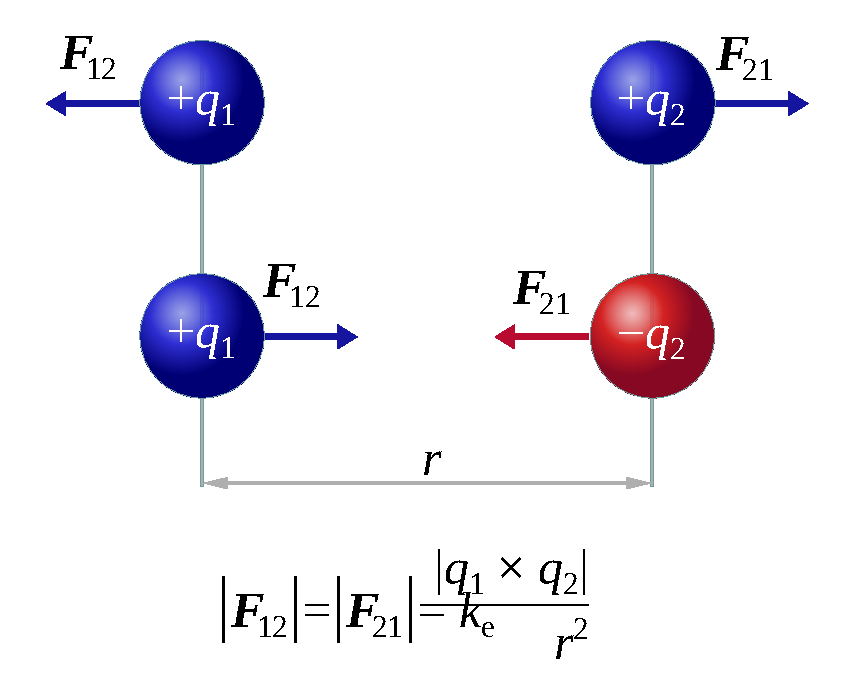
\includegraphics[scale=0.7]{CoulombsLaw}

    \caption{Signos en la Ley de Coulomb. Créditos: Wikipedia}
    \label{fig:canon_newton}
\end{figure}

El campo eléctrico generado por una partícula de carga $q$ es
\begin{align}
      \boldsymbol{E} =& k \frac{q}{r^3}\boldsymbol{r}\,,
\end{align}

% --- Inicio del código LaTeX para insertar ---

\begin{figure}[h!]
    \centering
    % Usamos minipage para colocar las dos figuras una al lado de la otra
    \begin{minipage}{0.48\textwidth}
        \centering
        % --- FIGURA IZQUIERDA: Carga Negativa ---
        \begin{tikzpicture}[
            scale=1.2, font=\large,
            charge/.style={circle, shade, ball color=blue, minimum size=1cm},
            equipotential/.style={dashed, green!50!black},
            fieldline/.style={->, >=Stealth, thick, red},
        ]
            % --- Dibujar la carga negativa en el centro ---
            \node[charge] at (0,0) {\textbf{--}};
            
            % --- Dibujar las líneas equipotenciales ---
            \foreach \r in {1, 2, 3} {
                \draw[equipotential] (0,0) circle (\r);
            }
            
            % --- Dibujar las líneas del campo eléctrico (hacia adentro) ---
            \foreach \angle in {0, 45, 90, 135, 180, 225, 270, 315} {
                \draw[fieldline] (\angle:3.5) -- (\angle:0.5);
            }
            
            % --- Añadir etiquetas ---
            \node[green!50!black, font=\small] at (0, 2.2) {Equipotencial};
            \node[red, font=\small, rotate=-45] at (45:2.5) {Campo $\boldsymbol{E}$};
        \end{tikzpicture}
        \caption*{a) Carga Negativa: Las líneas de campo apuntan radialmente hacia adentro.}
    \end{minipage}\hfill
    \begin{minipage}{0.48\textwidth}
        \centering
        % --- FIGURA DERECHA: Carga Positiva ---
        \begin{tikzpicture}[
            scale=1.2, font=\large,
            charge/.style={circle, shade, ball color=red, minimum size=1cm},
            equipotential/.style={dashed, green!50!black},
            fieldline/.style={->, >=Stealth, thick, blue},
        ]
            % --- Dibujar la carga positiva en el centro ---
            \node[charge] at (0,0) {\textbf{+}};
            
            % --- Dibujar las líneas equipotenciales ---
            \foreach \r in {1, 2, 3} {
                \draw[equipotential] (0,0) circle (\r);
            }
            
            % --- Dibujar las líneas del campo eléctrico (hacia afuera) ---
            \foreach \angle in {0, 45, 90, 135, 180, 225, 270, 315} {
                \draw[fieldline] (\angle:0.5) -- (\angle:3.5);
            }

            % --- Añadir etiquetas ---
            \node[green!50!black, font=\small] at (0, 2.2) {Equipotencial};
            \node[blue, font=\small, rotate=45] at (45:2.5) {Campo $\boldsymbol{E}$};
        \end{tikzpicture}
        \caption*{b) Carga Positiva: Las líneas de campo apuntan radialmente hacia afuera.}
    \end{minipage}
    
    \caption{Representación de las líneas del campo eléctrico ($\boldsymbol{E}$) y las superficies equipotenciales para una carga puntual negativa y una positiva. Las líneas de campo siempre son perpendiculares a las equipotenciales.}
    \label{fig:campos_electricos}
\end{figure}

% --- Fin del código LaTeX ---


Las magnitudes correspondientes para un par de cargas $q_1$ y $q_2$ son
\begin{align}
    F =& k\frac{q_1q_2}{r^2}\,,& E=& k\frac{q_1}{r^2} \,,
\end{align}
En este caso la carga $q_2$ corresponde a una carga de prueba para el  campo $E$ generado por $q_1$

%\newpage
\subsection{La Cantidad de Carga en un Grupo de Electrones}




\begin{examplebox}
    \textbf{Problema:} Calcule la carga, en coulombs, transportada por 6 mil millones de electrones.
\end{examplebox}

\vspace{5mm}

% --- CORRECCIÓN FINAL Y DEFINITIVA ---
% Usamos 'tabular' para la estructura general y 'array' para las ecuaciones.
\def\arraystretch{1.5} % Aumenta el espaciado vertical de las filas
\noindent % Asegura que la tabla ocupe todo el ancho
\begin{tabular}{|p{0.45\textwidth}|p{0.45\textwidth}|}
    \hline
    \textcolor{red}{\textbf{Razonamiento}} & \textcolor{red}{\textbf{Desarrollo}} \\
    \hline
    Exprese 6 mil millones (6 billion) en notación científica. & 
    % Usamos un entorno matemático y dentro un 'array' para alinear.
    \[
    \begin{array}{r@{\,}c@{\,}l} 
        1 \text{ mil millones} &=& 1 \times 10^9 \\
        6 \text{ mil millones} &=& 6 \times 10^9
    \end{array} 
    \] \\
    \hline
    Calcule la carga, $q$, en coulombs multiplicando el número de electrones por la carga de un electrón ($-1.6 \times 10^{-19}$~C). & 
    % Usamos un entorno matemático y dentro un 'array' para alinear.
    \[
    \begin{array}{r@{\,}c@{\,}l}
        q &=& (6 \times 10^9) \times (q_e) \\
          &=& (6 \times 10^9) \times (-1.6 \times 10^{-19} \, \text{C}) \\
          &=& -9.6 \times 10^{-10} \, \text{C}
    \end{array} 
    \] \\
    \hline
\end{tabular}
\def\arraystretch{1.0} % Restablece el valor por defecto

\vspace{1cm}

\textcolor{red}{\textbf{Ejemplo resuelto: Inténtalo tú mismo 12.1.1}}
\subsection*{La Cantidad de Carga en un Grupo de Electrones}

\begin{tcolorbox}[colframe=red, boxrule=1.5pt]
    \textbf{Problema:} Calcule la carga, en coulombs, transportada por 4 millones de electrones.
\end{tcolorbox}

% --- Fin del código LaTeX ---

% --- Inicio del código LaTeX para insertar ---

\subsection{Energía Potencial Electrostática ($U_e$)}

La \textbf{energía potencial electrostática ($U_e$)} de un sistema de dos cargas es una medida de la energía almacenada en el sistema debido a su configuración espacial. Se define como el \textbf{trabajo} que una fuerza externa debe realizar para traer una de las cargas (la carga de prueba, $q_2$) desde una posición de referencia en el infinito hasta una distancia $r$ de la otra carga ($q_1$), que se mantiene fija.

\subsection*{La Fórmula de la Energía Potencial}
La energía potencial generada por una carga fuente $q_1$ y sentida por una carga de prueba $q_2$ separadas por una distancia $r$ es:
\begin{equation}
    \boxed{
    U_e = k \frac{q_1 q_2}{r}
    }
    \label{eq:energia_potencial_e}
\end{equation}
\textbf{Notas importantes sobre la fórmula:}
\begin{itemize}
    \item A diferencia de la Ley de Coulomb para la magnitud de la fuerza, en esta ecuación los signos de las cargas $q_1$ y $q_2$ \textbf{son cruciales} y deben incluirse en el cálculo.
    \item La energía potencial decae como $1/r$, mientras que la fuerza decae como $1/r^2$.
\end{itemize}

\subsection*{Análisis de la Fórmula}
El signo de la energía potencial tiene una interpretación física directa:
\begin{description}
    \item[Si $U_e > 0$ (Repulsión):] Ocurre cuando $q_1$ y $q_2$ tienen el mismo signo. Se requiere un trabajo positivo (añadir energía al sistema) para juntar las cargas contra su repulsión natural. Si se sueltan, esta energía potencial se convertirá en energía cinética a medida que se alejan.

    \item[Si $U_e < 0$ (Atracción):] Ocurre cuando $q_1$ y $q_2$ tienen signos opuestos. El propio campo eléctrico realiza el trabajo para juntar las cargas. El sistema se encuentra en un estado ``ligado'' o en un ``pozo de potencial''. Se necesitaría realizar un trabajo externo positivo para separar las cargas y llevarlas al infinito.
\end{description}

\subsection*{Relación con el Potencial Eléctrico (Voltaje)}
El concepto de energía potencial está íntimamente ligado al de \textbf{potencial eléctrico ($V$)}, que es una propiedad del espacio creada por la carga fuente $q_1$. El potencial eléctrico se define como la energía potencial por unidad de carga:
\[ V = \frac{U_e}{q_2} \]
El potencial eléctrico creado por una carga puntual $q_1$ a una distancia $r$ es:
\[ V = k \frac{q_1}{r} \]
Con esta definición, podemos encontrar la energía potencial de cualquier carga de prueba $q_2$ colocada en un punto con potencial $V$ simplemente multiplicando:
\begin{align}
\label{eq:qV}
U_e = q_2 V
\end{align}
Esta relación es fundamental en el análisis de circuitos y campos electrostáticos.\footnote{Formalmente, la energía potencial es el negativo del trabajo realizado por la fuerza eléctrica para mover una carga desde el infinito: $U_e(r) = -\int_\infty^r \boldsymbol{F}_e \cdot d\boldsymbol{r}' = -\int_\infty^r (k \frac{q_1 q_2}{r'^2}) dr' = k \frac{q_1 q_2}{r}$.}

\subsection{El electronvoltio}
La energía potencial que adquiere un electrón al moverse a través de una diferencia de potencia de \qty{1}{V} es
\begin{align*}
    U_e = & V e = \qty{1}{V}\cdot \qty{1.602176634e-19}{\C} 
     =\qty{1.602176634e-19}{\joule}
\end{align*}
Esta cantidad de energía recibe el nombre de electronvoltio
\begin{align}
    \qty{1}{eV}\equiv\qty{1.602176634e-19}{\joule}\,.
\end{align}

% --- Fin del código LaTeX ---

% --- Inicio del código LaTeX para insertar ---

\subsection{Ejemplo Avanzado: Energía Potencial Eléctrica en el Núcleo de Uranio}

Ver libro: Destroyer of Worlds by Frank Close \url{}

Este ejemplo ilustra la escala de las energías involucradas a nivel nuclear y la inmensa fuerza de repulsión electrostática que la ``fuerza nuclear fuerte'' debe superar para mantener el núcleo unido. Además, se usa el hecho que para grandes núcleos es la fuerza eléctrica la que fuerza la fisión nuclear y entrega la energía cinética a las partes. 

Para entender esto, podemos pensar en los nucléos de los elementos químicos como gotas de un liquido muy denso que se mantiene cohesionado por la tensión superficial. La tensión superficial, $T$, es proporcional al área de la superficie sobre el volumen. Para un esfera
\begin{align*}
    T \propto \frac{\pi r^2}{\frac{4}{3}\pi r^3}
    \propto \frac{1}{r}\,,
\end{align*}
y por consiguiente disminuye con el radio. Esto hace por ejemplo que un bebe (volumen menor) necesite más abrigo que un adulto para controlar su temperatura corporal. En el caso de los núcleos implica que las ``gotas" prefieren fusionarse para el caso de núcleos livianos y fisionarse para el caso de núcleos pesados que tienden a deformarse más facilmente cuando reciben el impacto de un neutrón, como se ilustra en la figura~\ref{fig:gotas}

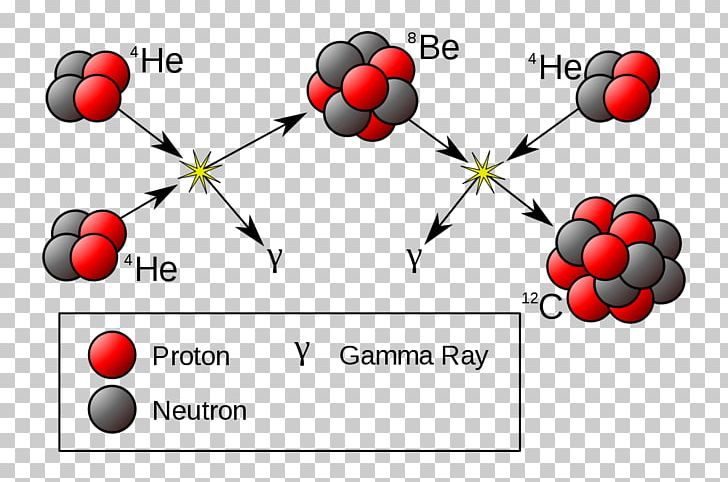
\includegraphics[scale=0.7]{fusion}

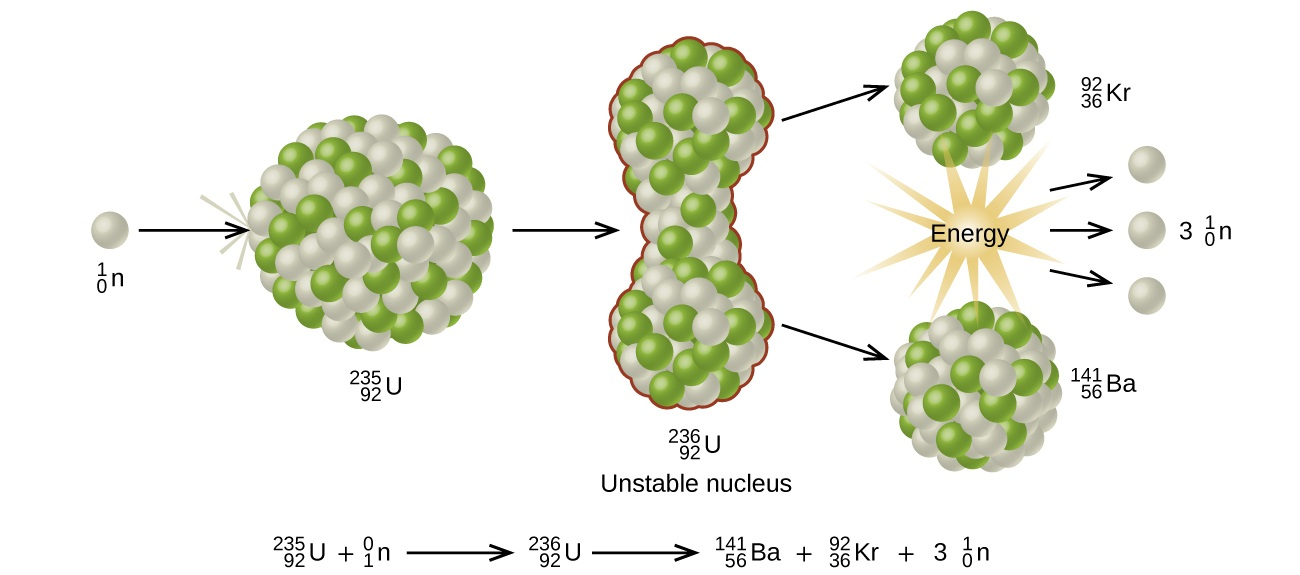
\includegraphics{gotas}

\subsection*{El Problema}
Calcular la energía potencial eléctrica total almacenada en un núcleo de Uranio-235 (${}^{235}_{92}\text{U}$) debido a la repulsión mutua de sus 92 protones. Luego, comparar esta energía con la de sus productos de fisión para entender la idea de Lise Meitner sobre la energía liberada.

\subsection*{El Error del ``Doble Conteo"}
% https://www.fisicalab.com/apartado/energia-potencial-electrica
Una primera intuición podría ser calcular la energía de un protón debida a los otros 91 y luego multiplicar por el número total de protones (92). Esto llevaría a una fórmula incorrecta de la forma $U_e \propto k \frac{(92e)(91e)}{R}$. Sin embargo, este método es erróneo porque cuenta la interacción de cada par de protones dos veces. La energía total de un sistema de cargas es el trabajo necesario para ensamblarlo, sumando la energía de cada \textbf{par único} de interacciones. Para un sistema complejo como un núcleo, la mejor aproximación es tratarlo como una esfera de carga uniforme.

\subsection*{Cálculo de la Energía Potencial Total del Núcleo de Uranio}
La energía potencial electrostática de una esfera de radio $R$ con una carga total $Q$ distribuida uniformemente es:
\begin{equation}
    U_{\text{esfera}} = \frac{3}{5} k \frac{Q^2}{R}\,.
\end{equation}
El factor 3/5 es, por tanto, un factor puramente geométrico que surge de la integración sobre el volumen de una esfera, ver apéndice~\ref{sec:3_5}. Ver también \url{https://www.feynmanlectures.caltech.edu/II_08.html}

La energía potencial es el trabajo realizado para, partiendo de un nucleón inicial, traer cada uno de los 92 protones desde el infinito. En la naturaleza éste trabajo fue realizado después de la colisión de las dos estrellas de neutrones que formaron nuestra protonebulosa planetaria. Se puede considerar entonces al Uranio como una batería natural donde se almacenó la energía gravitacional que permitió su creación. Esa energía se ha aprovechado a través de los reactores naturales que ocurrieron en momentos específicos de la historia terrestre (hace miles de millones de años) y en los reactores y bombas nucleares creados por el hombre.


\paragraph{Datos para el Uranio-235:}
\begin{itemize}
    \item Carga total, $Q = Z e = 92 \times \SI{1.602e-19}{\coulomb}$.
    \item Radio del núcleo, $R_U \approx (\SI{1.2}{\femto\meter}) \times A^{1/3} = (\SI{1.2e-15}{\meter}) \times (235)^{1/3} \approx \SI{7.41e-15}{\meter}$, donde $A$ es el número másico que es la suma de protones y neutrones en el núcleo de un átomo.
    \item Constante de Coulomb, $k \approx \SI{8.99e9}{\newton\meter\squared\per\coulomb\squared}$.
\end{itemize}

\paragraph{Cálculo:}
% --- CORRECCIÓN APLICADA AQUÍ ---
\begin{align*}
    U_{\text{Uranio}} &= \frac{3}{5} k \frac{(92e)^2}{R_U} \\
    &= \frac{3}{5} \times \num{8.99e9} \times \frac{(92 \times \num{1.602e-19})^2}{\num{7.41e-15}} \, \si{\joule} \\
    &\approx \num{1.58e-10} \, \si{\joule}
\end{align*}
Convirtiendo a Mega-electronvoltios (\SI{1}{\mega\electronvolt} = \SI{1.602e-13}{\joule}):
\[ U_{\text{Uranio}} \approx \frac{\SI{1.51e-10}{\joule}}{\SI{1.602e-13}{\joule\per\mega\electronvolt}} \approx \SI{986}{\mega\electronvolt} \]

\subsection*{La Genialidad de Lise Meitner: Comparando las Energías}
La idea clave de Meitner y Frisch fue comparar la energía del núcleo original con la suma de las energías de sus fragmentos de fisión, por ejemplo, Kriptón-92 (${}^{92}_{36}\text{Kr}$) y Bario-141 (${}^{141}_{56}\text{Ba}$) en la fisión
\begin{align*}
    {}^{235}_{92}\text{U} + n \to {}^{141}_{56}\text{Ba} + 
    + {}^{92}_{36}\text{Kr} + 3n\,.
\end{align*}

\paragraph{Energía de los Fragmentos:}
\begin{itemize}
    \item \textbf{Kriptón-92:} $Z=36, A=92 \implies R_{Kr} \approx \SI{5.4}{\femto\meter}$.
    \[ U_{Kr} = \frac{3}{5} k \frac{(36e)^2}{R_{Kr}} \approx \SI{200}{\mega\electronvolt} \]
    \item \textbf{Bario-141:} $Z=56, A=141 \implies R_{Ba} \approx \SI{6.2}{\femto\meter}$.
    \[ U_{Ba} = \frac{3}{5} k \frac{(56e)^2}{R_{Ba}} \approx \SI{450}{\mega\electronvolt} \]
\end{itemize}
La suma de la energía electrostática de los fragmentos es:
\[ U_{\text{fragmentos}} = U_{Kr} + U_{Ba} \approx \SI{200}{\mega\electronvolt} + \SI{450}{\mega\electronvolt} = \SI{650}{\mega\electronvolt} \]

\subsection*{Conclusión Final: La Fuente de la Energía de Fisión}
La diferencia entre la energía electrostática almacenada antes y después de la fisión es la energía que se libera.
\begin{itemize}
    \item Energía electrostática en el núcleo de Uranio: $\approx \SI{944}{\mega\electronvolt}$
    \item Energía electrostática en sus productos: $\approx \SI{650}{\mega\electronvolt}$
\end{itemize}
La diferencia de energía liberada es:
\[ \Delta E_{\text{electrostática}} = U_{\text{Uranio}} - U_{\text{fragmentos}} \approx \SI{986}{\mega\electronvolt} - \SI{650}{\mega\electronvolt} \approx \SI{336}{\mega\electronvolt} \]
Este valor, derivado puramente de la repulsión de Coulomb, se aproxima de manera sorprendente a la energía total liberada en una reacción de fisión (que experimentalmente es de unos \SI{200}{\mega\electronvolt}). Lise Meitner y Otto Frisch fueron los primeros en realizar este cálculo, explicando así el origen de la enorme cantidad de energía descubierta por Otto Hahn y Fritz Strassmann. El $85\%$ de esos $\qty{200}{MeV}$
se manifiesta cuando los dos nuevos núcleos creados salen disparados en direcciones opuestas a velocidades increíbles (alrededor del $3\%$ de la velocidad de la luz), y rozando fuertemente contra su entorno microscópico, produciendo un calor intenso.

El ${}^{235}_{92}\text{U}$ existe en nuestros días en una proporción del $0.7\%$ con respecto a ${}^{238}_{92}\text{U}$. En los reactores nucleares la principal reacción de éste último es la creación de plutonio a través de la captura de neutrones
\begin{align*}
    {}^{238}_{92}\text{U} + n\to {}^{239}_{92}\text{U}\,.
\end{align*}
El nuevo nucleo ${}^{239}_{92}\text{U}$ es muy inestable y sufre un decaimiento beta rápidamente (su vida media es de unos 23 minutos). Un neutrón se convierte en un protón
\begin{align*}
    {}^{239}_{92}\text{U} \to {}^{239}_{93}\text{Np}+e^- + \overline{\nu}_e\,.
\end{align*}
El Neptunio-239 (${}^{239}_{93}\text{Np}$) también es inestable y sufre otro decaimiento beta (su vida media es de unos 2.4 días).
\begin{align*}
{}^{239}_{93}\text{Np} \to {}^{239}_{94}\text{Pu} + e^- + \overline{\nu}_e\,.   
\end{align*}
Resultado: Se ha creado un nuevo elemento, el Plutonio-239 (${}^{239}_{94}\text{Pu}$). Note que los nombres de estos dos elementos de la tabla períodica reciben su nombre a semejanza de cuando había nueve planetas y teníamos a Urano, Neptuno y Plutón. 


\subsubsection{La Naturaleza Electrostática de los Enlaces Químicos}

Habiendo estudiado la Ley de Coulomb y la energía potencial electrostática ($U_e$), podemos comprender uno de los fenómenos más importantes del universo: cómo y por qué se unen los átomos para formar la materia que nos rodea. En última instancia, toda la química —desde la formación de una simple molécula de agua hasta la compleja estructura del ADN— no es más que una manifestación directa de las interacciones electrostáticas.

Cuando dos átomos se acercan, interactúan sus nubes de electrones (con carga negativa) y sus núcleos (con carga positiva). Dependiendo de cómo se redistribuyan estos electrones para minimizar la energía potencial del sistema, surgen diferentes tipos de enlaces, todos gobernados por la fuerza eléctrica.

\paragraph{1. Enlace Iónico: La Atracción Directa}
En un enlace iónico (como en la sal de mesa, NaCl), un átomo cede completamente uno o más electrones a otro. Esto genera dos iones: un catión (carga positiva) y un anión (carga negativa). 
La física de este enlace es la más sencilla de modelar algebraicamente. Una vez formados los iones, experimentan una atracción puramente coulómbica que los mantiene unidos en una red cristalina. La energía potencial que los une es extremadamente negativa (lo que implica un estado muy estable) y se describe mediante nuestra fórmula ya conocida:
\begin{equation}
    U_e = -k \frac{|q_1| |q_2|}{r}.
\end{equation}

\paragraph{2. Enlace Covalente: El Equilibrio de Fuerzas}
En muchas moléculas (como el gas hidrógeno, $\text{H}_2$), los átomos no ceden electrones, sino que los ``comparten''. Físicamente, esto significa que los electrones compartidos se ubican en el espacio \textit{entre} los dos núcleos positivos.

Para entender por qué esto mantiene unidos a los átomos, debemos analizar el balance de las fuerzas electrostáticas (ver Figura \ref{fig:enlace_covalente}).

\begin{figure}[htbp]
\centering
\begin{tikzpicture}[>=stealth, scale=1.2]
    
    % Núcleos (Protones)
    \coordinate (N1) at (-2.5, 0);
    \coordinate (N2) at (2.5, 0);
    
    % Electrones compartidos (en el centro)
    \coordinate (E1) at (0, 0.4);
    \coordinate (E2) at (0, -0.4);

    % Dibujar núcleos
    \draw[fill=red!20, draw=red, thick] (N1) circle (0.3) node[text=red!80!black] {$+$};
    \draw[fill=red!20, draw=red, thick] (N2) circle (0.3) node[text=red!80!black] {$+$};
    
    % Dibujar electrones
    \draw[fill=blue!20, draw=blue, thick] (E1) circle (0.15) node[text=blue!80!black, font=\scriptsize] {$-$};
    \draw[fill=blue!20, draw=blue, thick] (E2) circle (0.15) node[text=blue!80!black, font=\scriptsize] {$-$};

    % Nube electrónica compartida (esquemática)
    \draw[dashed, blue, thick, opacity=0.5] (0,0) ellipse (1.2 and 1);

    % Fuerzas de REPULSIÓN (Rojas, hacia afuera)
    \draw[->, ultra thick, red!80!black] (N1) ++(-0.4, 0) -- ++(-1, 0) node[above] {$\boldsymbol{F}_{\text{repulsión}}$};
    \draw[->, ultra thick, red!80!black] (N2) ++(0.4, 0) -- ++(1, 0) node[above] {$\boldsymbol{F}_{\text{repulsión}}$};

    % Fuerzas de ATRACCIÓN (Azules, hacia el centro)
    \draw[->, ultra thick, blue!80!black] (N1) ++(0.35, 0.1) -- (E1) node[midway, above left, font=\scriptsize] {$\boldsymbol{F}_{\text{atracción}}$};
    \draw[->, ultra thick, blue!80!black] (N1) ++(0.35, -0.1) -- (E2);
    
    \draw[->, ultra thick, blue!80!black] (N2) ++(-0.35, 0.1) -- (E1) node[midway, above right, font=\scriptsize] {$\boldsymbol{F}_{\text{atracción}}$};
    \draw[->, ultra thick, blue!80!black] (N2) ++(-0.35, -0.1) -- (E2);

\end{tikzpicture}
\caption{Modelo electrostático de un enlace covalente (por ejemplo, $\text{H}_2$). Los dos núcleos positivos se repelen mutuamente. Sin embargo, los electrones ubicados en la región central atraen a ambos núcleos simultáneamente. Si la fuerza de atracción atractiva combinada supera a la repulsión nuclear, la molécula es estable.}
\label{fig:enlace_covalente}
\end{figure}

El sistema alcanza un estado estable únicamente cuando la distancia entre los núcleos es tal que la enorme energía de repulsión entre ellos ($+U_e$) es compensada e incluso superada por la energía de atracción hacia los electrones centrales ($-U_e$). En términos de fuerzas, la molécula no se desintegra porque la fuerza neta sobre cada núcleo es cero:
\begin{equation}
    \sum \boldsymbol{F}_{\text{sobre un núcleo}} = \boldsymbol{F}_{\text{repulsión (núcleo-núcleo)}} + \boldsymbol{F}_{\text{atracción (núcleo-electrones)}} = \boldsymbol{0}.
\end{equation}

\paragraph{3. Enlace Metálico: El ``Mar'' de Electrones}
En un trozo de metal sólido (como un cable de cobre), los átomos liberan sus electrones más externos. Esto deja una red tridimensional rígida de cationes positivos sumergidos en un fluido o ``mar'' de electrones negativos con gran movilidad. La atracción electrostática entre los iones positivos y este fluido negativo cohesiona el metal. Es precisamente la tremenda movilidad de estas cargas en el espacio libre de la red lo que hace que los metales sean excelentes conductores de la corriente eléctrica (tema que abordaremos en la siguiente sección).

\paragraph{4. Interacciones Intermoleculares: Dipolos Permanentes y Fuerzas de Van der Waals}

Incluso las moléculas que son globalmente neutras (cuya carga total es cero) experimentan fuerzas eléctricas que determinan sus estados físicos. Esto ocurre debido a la distribución asimétrica de la carga en el espacio.

Por un lado, tenemos moléculas con \textbf{dipolos permanentes} (como el agua, $\text{H}_2\text{O}$). En estas moléculas covalentes, los electrones no se comparten de forma equitativa. Se acumulan más cerca de un átomo (como el oxígeno) dándole una carga parcial negativa ($\delta^-$), y dejando a los otros átomos (los hidrógenos) con una carga parcial positiva ($\delta^+$). La atracción electrostática entre el extremo positivo de una molécula y el extremo negativo de su vecina genera uniones como los llamados ``puentes de hidrógeno''.

Por otro lado, existen las \textbf{Fuerzas de Van der Waals} (específicamente las fuerzas de dispersión de London). Estas son las interacciones electrostáticas más sorprendentes, ya que explican cómo pueden atraerse moléculas que son completamente apolares y simétricas (como el gas nitrógeno, $\text{N}_2$, o los gases nobles). 
¿De dónde surge la fuerza eléctrica si la molécula no tiene polos positivos ni negativos fijos?

La respuesta reside en el movimiento constante de los electrones. Aunque en promedio la nube electrónica es simétrica, en cualquier instante infinitesimal de tiempo ($t_0$), los electrones pueden encontrarse casualmente agrupados hacia un lado del átomo o molécula. Esto crea un \textbf{dipolo instantáneo} efímero. 
La física electrostática nos dice que este polo negativo temporal repelerá a los electrones de las moléculas vecinas, induciendo en ellas un \textbf{dipolo inducido} con la polaridad opuesta.

De forma algebraica, aunque cada carga involucrada es parcial ($\delta$), la ley de Coulomb sigue dictando la interacción atractiva neta entre estos diminutos polos enfrentados:
\begin{equation}
    |\boldsymbol{F}_{\text{Van der Waals}}| \propto \frac{|\delta^+| |\delta^-|}{r^7}.
\end{equation}
\textit{(Nota: La fuerza de Van der Waals decae con la distancia mucho más rápido ($1/r^7$) que la fuerza de Coulomb estándar entre cargas puntuales puras ($1/r^2$), debido a la compleja geometría de la interacción entre dipolos oscilantes).}

Aunque son las interacciones electrostáticas más débiles, estas fuerzas son responsables de condensar los gases nobles en líquidos a muy bajas temperaturas y son el secreto biológico detrás de la capacidad de los lagartos gecko (cuyas patas tienen millones de pelillos microscópicos) para trepar por paredes de cristal mediante pura atracción eléctrica.



\section{Corriente eléctrica}
\begin{align}
    I =\frac{q}{t}
\end{align}

La corriente eléctrica está conformada típicamente por electrones en movimiento. En tal caso $q=n_e q_e$
\begin{align}
    I = \frac{n_e q_e}{t}\,,
\end{align}
donde $n_e$ es el número de electrones y $q_e$ la carga del electrón.

De \eqref{eq:qV},
\begin{align}
   W = U_e =& V q\nonumber\\
           = & V \frac{q}{t} t\nonumber\\
           = & V I t\,.
\end{align}

\begin{align}
    P = \frac{W}{t},,
\end{align}
Por consiguiente
\begin{align}
    P = VI,,
\end{align}
donde
\begin{itemize}
    \item $P$ es la potencia
    \item  $V$ es el Potencial eléctrico (realmente la diferencia de potencial), llamado coloquialmente el 
    \emph{Voltaje}
    \item $I$ es la corriente eléctrica
\end{itemize}

\newpage
\textbf{Ejemplo:} Calcule el número de electrones que fluyen por un punto particular cada segundo en un cable de cobre que transporta una corriente de $0.5 \text{ A}$.

\begin{table}[htbp]
\centering
\renewcommand{\arraystretch}{1.5}
\begin{tabular}{|p{0.5\textwidth}|p{0.45\textwidth}|}
\hline
\textbf{\textcolor{red}{Razonamiento}} & \textbf{\textcolor{red}{Desarrollo}} \\
\hline
Reorganice la ecuación $I = \frac{q}{t}$ para despejar $q$. & 
$\begin{aligned}
    I &= \frac{q}{t} \\
    I \times t &= \left(\frac{q}{t}\right) \times t \\
    \therefore q &= I \times t
\end{aligned}$ \\
\hline
Calcule la cantidad de carga que fluye por el punto en cuestión sustituyendo los valores dados. & 
$\begin{aligned}
    q &= 0.5 \times 1 \\
      &= 0.5 \text{ C}
\end{aligned}$ \\
\hline
Encuentre el número de electrones dividiendo la carga entre la carga de un electrón ($1.6 \times 10^{-19} \text{ C}$). & 
$\begin{aligned}
    n_e &= \frac{q}{q_e} \\
        &= \frac{0.5}{1.6 \times 10^{-19}} \\
        &= 3.13 \times 10^{18} \text{ electrones.}
\end{aligned}$ \\
\hline
\end{tabular}
\end{table}

% --- Inicio del código LaTeX para insertar ---

\subsection{Ejemplo: Cálculo de la potencia eléctrica}
Usando  $P = V I$

Un equipo funcionando a $\qty{110}{V}$  usa una corriente de $\qty{4}{A}$.
Calcular la potencia usada por el equipo: ver tabla~\ref{tab:potencia_electrica_es}.

\begin{table}[h!]
\centering
\caption{Cálculo de la potencia eléctrica.}
\label{tab:potencia_electrica_es}
\renewcommand{\arraystretch}{1.5} % Aumenta el espaciado vertical
\begin{tabular}{|p{0.45\textwidth}|l|}
\hline
\textcolor{red}{\textbf{Razonamiento}} & \textcolor{red}{\textbf{Desarrollo}} \\
\hline
Identificar la relación necesaria para resolver el problema. & 
    $\displaystyle P = VI$ \\
\hline
Identificar los valores requeridos de la pregunta, sustituir y calcular. & 
    % Usamos un entorno align* dentro de un minipage para evitar errores
    \begin{minipage}[t]{0.45\textwidth}
    \[\begin{aligned}
        P &= VI \\
          &= 110 \times 4 \\
          &= \SI{440}{\watt}
    \end{aligned}\]
    \end{minipage} \\
\hline
\end{tabular}
\end{table}

\subsection{Consumo de energía}
Considere la etiqueta para el consumo de energía de un electrodoméstico mostrada en la figura~\ref{fig:nevera}. Calcule la potencia utilizada por el electrodoméstico.

\begin{figure}[h!]
    \centering
    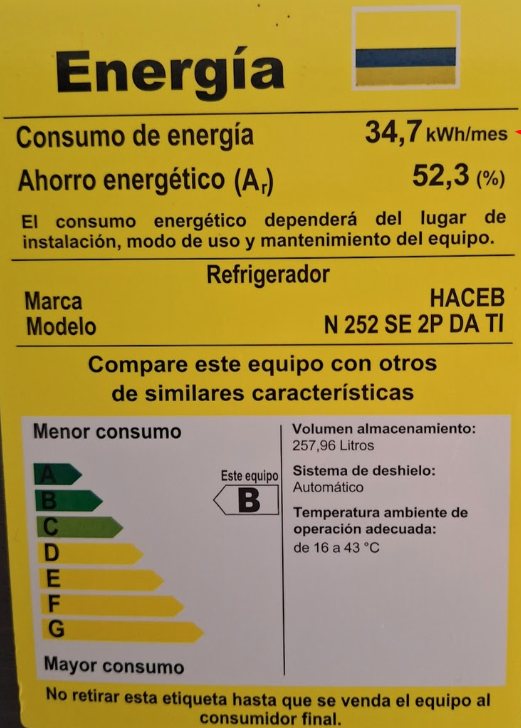
\includegraphics[scale=0.3]{consumo}
    \caption{Consumo de energía de una nevera}
    \label{fig:nevera}
\end{figure}

\begin{align*}
    P = &{34.7}{\frac{\cancel{\text{kW}}\cancel{\text{h}}}{\cancel{\text{mes}}}}
    \left(\frac{\qty{1}{\cancel\month}}{\qty{720}{\cancel\hour}}\right)\frac{\qty{1000}{\watt}}{1\,\cancel{\text{kW}}}\\
    =& \qty{48}{\watt}
\end{align*}

La correspondiente corriente es
\begin{align*}
    I =& \frac{P}{V}\\
     = &\frac{\qty{48}{\watt}}{\qty{110}{\volt}}\\
       =& \qty{0.44}{\ampere}\,.
\end{align*}

% --- Inicio del código LaTeX para insertar ---

\subsection{Ejemplo: Cálculo de la Potencia Media a partir de la Factura de Servicios}

\paragraph{Enunciado del Problema:}
Si la cuenta de servicios de un hogar registra en un mes un consumo de energía de \qty{191}{\kilo\watt\hour}, ¿cuál fue la potencia media utilizada por la casa durante ese mes?

\subsection*{Solución Detallada}

\paragraph{1. Entender los Conceptos:}
Este problema nos pide encontrar la \textbf{potencia media}, que es la tasa constante a la que se habría consumido energía durante el mes. La factura nos proporciona la \textbf{energía total} consumida.
\begin{itemize}
    \item Energía Total Consumida, $U_e = \qty{191}{\kilo\watt\hour}$.
    \item Potencia Media, $P = \text{?}$
\end{itemize}

\paragraph{2. Fórmula de Relación:}
La relación fundamental entre energía, potencia y tiempo es $E = P \times t$. Para encontrar la potencia media, despejamos la fórmula:
\[ P = \frac{U_e}{t} \]

\paragraph{3. Calcular el Tiempo Total en Horas:}
Necesitamos el número total de horas en un mes. Asumiremos un mes promedio de 30 días y usaremos factores de conversión en modo fraccionario.
\begin{align*}
    t &= \qty{30}{días} \times \left( \frac{\qty{24}{horas}}{\qty{1}{día}} \right) \\
      &= \qty{720}{horas}
\end{align*}

\paragraph{4. Calcular la Potencia Media:}
Ahora, aplicamos la fórmula sustituyendo la energía y el tiempo total:
\[ P_{\text{media}} = \frac{\qty{191}{\kilo\watt\hour}}{\qty{720}{h}} \]
Las unidades de horas (h) en el numerador y el denominador se cancelan, dejándonos con kilovatios (kW):
\[ P_{\text{media}} \approx \qty{0.2653}{\kilo\watt} \]

\paragraph{5. Convertir a Watts (W):}
Para una interpretación más intuitiva, convertimos el resultado a vatios.
\begin{align*}
    P_{\text{media}} &= \qty{0.2653}{\kilo\watt} \times \left( \frac{\qty{1000}{W}}{\qty{1}{kW}} \right) \\
                     &\approx \qty{265.3}{\watt}
\end{align*}

\subsection*{Conclusión}
La potencia media consumida por la casa durante ese mes fue de aproximadamente \textbf{\qty{265}{\watt}}. Esto es equivalente al consumo continuo de, por ejemplo, un refrigerador moderno y varios dispositivos electrónicos pequeños funcionando las 24 horas del día.

% --- Fin del código LaTeX ---

% --- Fin del código LaTeX ---

\section{Magnetismo}

% --- Inicio del código LaTeX para insertar (versión simple) ---

El \textbf{campo magnético ($\boldsymbol{B}$)} es una cantidad vectorial, ya que tiene tanto una magnitud como una dirección.

La intensidad, o magnitud del vector, del campo magnético está en unidades de \textbf{tesla (T)} y se denota con la variable $B$.

Un imán genera un campo magnético de tipo dipolar similar al campo eléctrico que generan dos partículas cargadas de cargas opuestas como se muestra en la figura~\ref{fig:magnetismo}

\begin{figure}[h!]
    \centering
    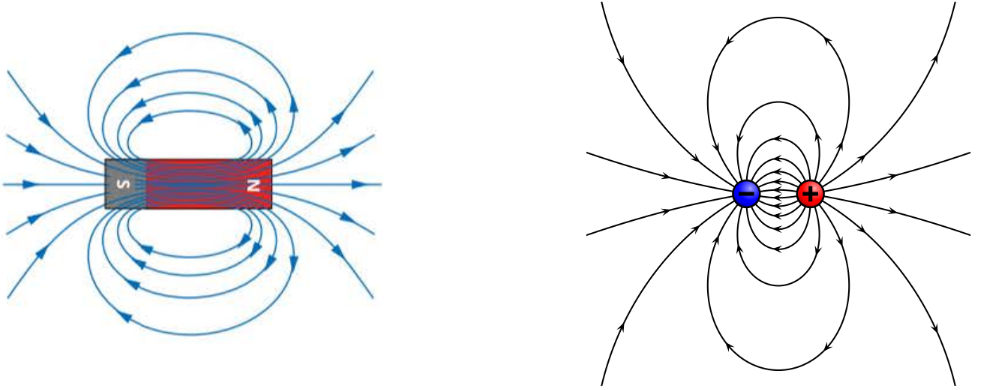
\includegraphics[scale=0.45]{dipolar}
    \caption{Campo dipolar}
    \label{fig:magnetismo}
\end{figure}

% --- Fin del código LaTeX ---

\section{Ley de Ampère}
En electrostática, vimos que las cargas eléctricas generan campos eléctricos. En magnetismo, la regla fundamental descubierta por André-Marie Ampère establece que \textbf{las corrientes eléctricas (cargas en movimiento) generan campos magnéticos}. 

Para calcular la magnitud de este campo magnético sin recurrir a matemáticas avanzadas (como el cálculo integral), podemos utilizar una formulación geométrica y puramente algebraica de la Ley de Ampère. 

Imaginemos un ``lazo cerrado'' imaginario (como una banda elástica geométrica) de longitud total $L$, que envuelve a una o varias corrientes eléctricas. Si el campo magnético $\boldsymbol{B}$ es constante a lo largo de este lazo y apunta siempre paralelo a él, la Ley de Ampère nos dice que el producto del campo por la longitud del lazo es directamente proporcional a la \textbf{corriente total encerrada} ($I_{\text{enc}}$) por dicho lazo:
\begin{equation}
    B \cdot L = \mu_0 I_{\text{enc}},
    \label{eq:ampere_algebraica}
\end{equation}
donde $\mu_0 = 1.257 \times 10^{-6} \text{ T}\cdot\text{m/A}$ es la permeabilidad magnética del vacío, una constante universal que dicta qué tan fácil es establecer un campo magnético en el espacio vacío.

Esta sencilla ecuación algebraica nos permite deducir inmediatamente las fórmulas para los campos magnéticos en diferentes geometrías cotidianas.

\subsection{El Campo de un Alambre Recto}

Imaginemos un cable recto y muy largo que transporta una corriente $I$. La simetría del cable nos dicta que el campo magnético $\boldsymbol{B}$ formará círculos perfectos a su alrededor, , como se muestra en la figura~\ref{fig:ampere}.

\begin{figure}[h!]
    \centering
    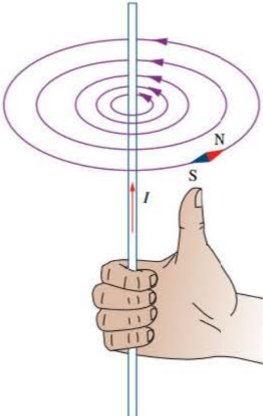
\includegraphics[scale=0.7]{ampere}
    \caption{Ley de Ampère}
    \label{fig:ampere}
\end{figure}


Si queremos calcular el campo a una distancia $r$ del cable, nuestro ``lazo imaginario'' será un círculo de radio $r$. La longitud total de este lazo cerrado es la circunferencia del círculo, es decir, $L = 2\pi r$. La corriente que atraviesa o ``perfora'' el interior de este círculo es simplemente $I_{\text{enc}} = I$.

Sustituyendo estos valores geométricos en nuestra formulación algebraica de la Ley de Ampère (Ecuación \ref{eq:ampere_algebraica}), obtenemos
\begin{equation}
    B \cdot (2\pi r) = \mu_0 I.
\end{equation}
Despejando algebraicamente el campo magnético $B$, recuperamos la famosa fórmula para un alambre:
\begin{equation}
    B = \frac{\mu_0 I}{2\pi r}.
\end{equation}
donde
\begin{itemize}
    \item $B$ es la magnitud del campo magnético (en T)
    \item $\mu_0 = \qty{1.257e-6}{NA^{-2}}$ es la permeabilidad del vacío 
    \item $I$ es la corriente (en A)
    \item $r$ es la distancia desde el alamabre (en m).
\end{itemize}

Este resultado nos muestra que el campo magnético decae a medida que nos alejamos del cable (inversamente proporcional a la distancia $r$).
Cuando una carga eléctrica se mueve o gira sobre sí misma, genera un campo magnético. 


% --- Fin del código LaTeX ---

Cuando una carga de prueba, $q$, se mueve con un velocidad $\boldsymbol{v}$ en presencia de un campo magnético $\boldsymbol{B}$, se genera una fuerza dada por
\begin{align}
    \boldsymbol{F} = q \boldsymbol{v}\times \boldsymbol{B}
\end{align}
con magnitud
\begin{align}
    F = q v B\sin\theta\,,
\end{align}
donde $\theta$ es el ángulo formado entre los vectores $\boldsymbol{v}$ y $\boldsymbol{B}$. Para obtener  la dirección del vector de fuerza, 
los vectores $\boldsymbol{v}$, $\boldsymbol{B}$ y $\boldsymbol{F}$ conforman una tripleta de mano derecha (ver figura~\ref{fig:manoderecha}) lo cual quiere decir que si el dedo meñique con la mano extendida señala la dirección de la velocidad, al enrollar la mano buscando la dirección del vector del campo magnético, el dedo pulgar indica la dirección de la fuerza resultante.


La magnitud de la fuerza que la corriente $I_1$ ejerce sobre una carga $q_2$ que fluye con la corriente $I_2$ a una velocidad $\boldsymbol{v}$, para recorrer la distancia $L$ en un tiempo $t$, está ilustrada en la figura~\ref{fig:alambres}

\begin{figure}
    \centering
    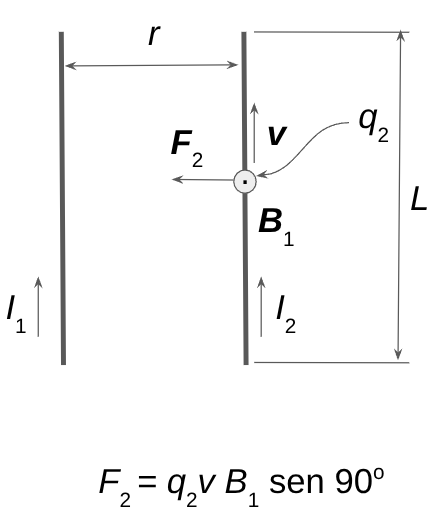
\includegraphics[scale=0.7]{alambres}
    \caption{Fuerza  sobre una partícula con carga $q_2$ que se mueve a velocidad $\boldsymbol{v}$ sometida a un campo magnético $\boldsymbol{B}$}
    \label{fig:alambres}
\end{figure}


\begin{align*}
F_2 =& q_2 v B_1\\
=& q_2\frac{L}{t} B_1\\
=& \frac{q_2}{t} L B_1\\
=& I_2 L B_1\,.
\end{align*}

Reemplazando la magnitud del campo magnético 
a una distancia $r$ del alambre con corriente $I_1$ (donde se encuentra el alambre con corriente $I_2$) dado por

\begin{align*}
    B_1 = \frac{\mu_0 I_1}{2\pi r}\,,
\end{align*}

tenemos que la magnitud fuerza por unidad de longitud que ejerce $I_1$ sobre $I_2$ es

\begin{align*}
    \frac{F_2}{L} = \frac{\mu_0 I_1 I_2}{2\pi r}\,,
\end{align*}

en la dirección hacia el cable con corriente $I_1$, como se muestra en la figura.

De aquí observamos que el campo magnético es una fuerza temporaloide que varía con el inverso del tiempo al cuadrado, y además, quedan claro las unidades de 
\begin{align*}
    \left[\mu_0\right] = \unit{N A^{-2}}
\end{align*}

En general, para encontrar la fuerza actuando sobre un conductor cuando la corriente se mueve a un ángulo  $\theta$ con el vector de campo magnético, esta dada por
\begin{equation}
    F = L I B \sin\theta\,,
\end{equation}
donde
\begin{itemize}
    \item $F$ es la fuerza sobre el conductor ($\unit{N}$)
    \item $L$ es la longitud del conductor ($\unit{\m}$)
    \item $I$ es la corriente en el conductor ($\unit{A}$)
    \item $B$ es la intensidad del campo magnético ($\unit{T}$)
    \item $\theta$ es el ángulo entre el campo magnético y el conductor.
\end{itemize}


\subsubsection{Aplicación Práctica: El Motor Eléctrico}

La electricidad puede generar movimiento mecánico. Este es el principio de funcionamiento de un \textbf{motor eléctrico}, y está gobernado por la fuerza magnética sobre un conductor, la cual derivamos anteriormente:
\begin{equation}
    F = L I B \sin\theta.
\end{equation}

\subsubsection{El Mecanismo de Rotación (Fuerza y Torque)}

Un motor eléctrico básico de corriente continua (DC) consiste en una espira rectangular de alambre (el \textit{rotor}) montada sobre un eje de rotación, y situada entre los polos norte y sur de un imán permanente (el \textit{estator}), como se muestra en la Figura \ref{fig:motor_electrico}.

\begin{figure}[htbp]
\centering
\begin{tikzpicture}[>=stealth, scale=1.3]
    
    % Polos Magnéticos (Estator)
    \draw[thick, fill=red!70!black] (-2.5, -1) rectangle (-1.5, 1);
    \node[text=white, font=\large\bfseries] at (-2, 0) {N};
    
    \draw[thick, fill=blue!70!black] (1.5, -1) rectangle (2.5, 1);
    \node[text=white, font=\large\bfseries] at (2, 0) {S};

    % Líneas de Campo Magnético (B)
    \foreach \y in {-0.6, 0, 0.6} {
        \draw[->, thick, gray, dashed] (-1.5, \y) -- (1.5, \y);
    }
    \node[gray, above] at (0, 0.6) {$\boldsymbol{B}$};

    % Espira del Rotor (En perspectiva)
    \coordinate (A) at (-0.8, -0.4);
    \coordinate (B) at (-0.8, 0.8);
    \coordinate (C) at (0.8, 0.4);
    \coordinate (D) at (0.8, -0.8);
    
    \draw[ultra thick, orange!80!black] (A) -- (B) node[midway, left] {$L$};
    \draw[ultra thick, orange!80!black] (B) -- (C);
    \draw[ultra thick, orange!80!black] (C) -- (D);
    \draw[ultra thick, orange!80!black] (D) -- (0.8, -1.2);
    \draw[ultra thick, orange!80!black] (A) -- (-0.8, -1.2);

    % Eje de rotación
    \draw[thick, black, dash dot] (0, 1.5) -- (0, -1.5);
    \draw[->, thick] (0, 1.3) arc (90:400:0.2 and 0.05);
    \node[above] at (0, 1.5) {Eje de rotación};

    % Corriente (I)
    \draw[->, thick, black] (-0.8, -0.2) -- (-0.8, 0.3) node[midway, right] {$I$};
    \draw[->, thick, black] (0.8, 0.2) -- (0.8, -0.3) node[midway, left] {$I$};

    % Fuerzas (F)
    % Fuerza en el cable izquierdo (Hacia ARRIBA/AFUERA en 3D, dibujada hacia arriba)
    \draw[->, ultra thick, purple] (-0.8, 0.2) -- (-0.8, 1.5) node[above] {$\boldsymbol{F}_1$};
    % Fuerza en el cable derecho (Hacia ABAJO/ADENTRO en 3D, dibujada hacia abajo)
    \draw[->, ultra thick, purple] (0.8, -0.2) -- (0.8, -1.5) node[below] {$\boldsymbol{F}_2$};

\end{tikzpicture}
\caption{Esquema básico de un motor eléctrico. Una corriente $I$ fluye por una espira de alambre dentro de un campo magnético $\boldsymbol{B}$. Por la regla de la mano derecha, la corriente que sube por el lado izquierdo experimenta una fuerza $\boldsymbol{F}_1$ en una dirección, mientras que la corriente que baja por el lado derecho experimenta una fuerza $\boldsymbol{F}_2$ en la dirección opuesta. Este par de fuerzas genera un \textbf{torque} que hace girar el motor.}
\label{fig:motor_electrico}
\end{figure}

Para entender por qué gira el motor, aplicamos la física por partes:
\begin{enumerate}
    \item \textbf{La Corriente y el Campo:} La batería empuja una corriente $I$ que sube por el segmento izquierdo de la espira y baja por el segmento derecho. Todo el conjunto está sumergido en un campo magnético constante $\boldsymbol{B}$ que apunta del polo Norte al polo Sur.
    \item \textbf{La Fuerza de Lorentz:} Aplicamos la Ecuación $F = LIB \sin(90^\circ)$ a los segmentos verticales. Usando la regla de la mano derecha (dedos en dirección de $I$, doblando hacia $\boldsymbol{B}$), encontramos que sobre el cable izquierdo actúa una fuerza $\boldsymbol{F}_1$ hacia "afuera", y sobre el cable derecho actúa una fuerza $\boldsymbol{F}_2$ igual de intensa pero hacia "adentro".
    \item \textbf{Generación del Torque:} Como vimos en el Capítulo 3, dos fuerzas paralelas que apuntan en sentidos opuestos y aplicadas a cierta distancia de un pivote no cancelan su efecto rotacional; por el contrario, se suman para generar un \textbf{torque} ($\boldsymbol{\tau} = \boldsymbol{r} \times \boldsymbol{F}$). Es este torque el que obliga a la espira a girar incesantemente alrededor de su eje central.
\end{enumerate}

\textbf{Conclusión Tecnológica:} 
El motor eléctrico es la máxima demostración de cómo el álgebra vectorial rige la tecnología moderna. Al invertir ingeniosamente la dirección de la corriente cada media vuelta (mediante unos contactos llamados \textit{conmutadores}), los ingenieros aseguran que el torque siempre empuje en la misma dirección rotacional, transformando así la energía eléctrica en trabajo mecánico continuo.


\subsection{Campo magnético alrededor de un solenoide}  

Si se colocan muchas espiras una al lado de la otra, sus campos se suman y el efecto es mucho más intenso. Esto se logra fácilmente enrollando muchas vueltas de alambre en una bobina denominada solenoide. El campo alrededor del solenoide es similar al campo alrededor de un imán de barra normal. La dirección del campo magnético total se puede determinar considerando el campo alrededor de cada espira y, a su vez, el campo alrededor del alambre portador de corriente que forma la espira. La dirección del campo del solenoide depende de la dirección de la corriente en el alambre que lo compone.

Como se muestra en la figura~\ref{fig:solenoide}, el solenoide tiene el polo norte a la izquierda y el sur a la derecha. Una brújula debería apuntar en la dirección que se indica en la figura~\ref{fig:solenoide}.

\begin{figure}
    \centering
    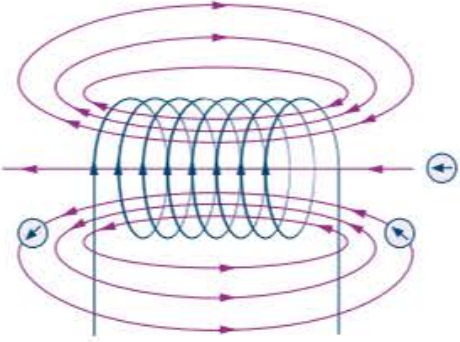
\includegraphics[scale=0.6]{solenoide}
    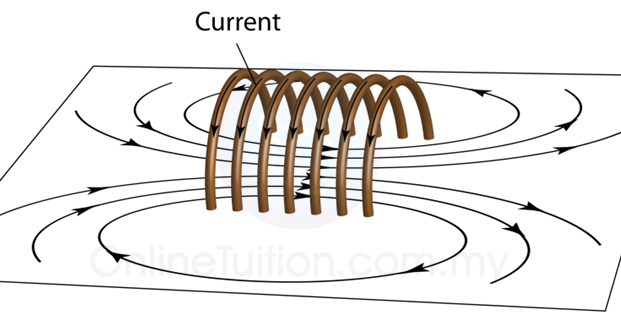
\includegraphics[scale=0.3]{solenoide2}
    \caption{Campo magnético generado por la corriente circulando por un solenoide}
    \label{fig:solenoide}
\end{figure}

Un electroimán, como su nombre lo indica, funciona con electricidad. Su funcionamiento se basa en que una corriente eléctrica produce un campo magnético alrededor de un alambre portador de corriente. Si el conductor se enrolla en una serie de bobinas para formar un solenoide, el campo magnético se concentra dentro de las bobinas. Cuantas más bobinas, más fuerte es el campo magnético y, por lo tanto, más fuerte es el electroimán.
El campo magnético se puede intensificar aún más enrollando las bobinas alrededor de un núcleo. Normalmente, los átomos en materiales como el hierro apuntan en direcciones aleatorias y sus campos magnéticos individuales tienden a cancelarse entre sí. Sin embargo, el campo magnético producido por las bobinas enrolladas alrededor de un núcleo de hierro obliga a los átomos dentro del núcleo a apuntar en una sola dirección. Sus campos magnéticos individuales se suman, creando un campo magnético más fuerte. Esto es similar al concepto de fabricar un imán permanente.
La intensidad de un electroimán también se puede cambiar variando la cantidad de corriente eléctrica que fluye a través de él.
La dirección de la corriente crea polos en el electroimán. Los polos de un electroimán se pueden invertir invirtiendo la dirección de la corriente eléctrica.
Hoy en día, los electroimanes se utilizan directamente para levantar objetos pesados, como interruptores y relés, y como una forma de crear nuevos imanes permanentes al alinear los átomos dentro de materiales magnéticos.

Un solenoide es una bobina formada por un cable enrollado en forma de espiral con $N$ vueltas (espiras) a lo largo de una longitud física $L_{\text{bobina}}$. ¿Cuál es el campo magnético en su interior?


\subsubsection{Campo magnético al interior de un solenoide}

Para entender de dónde sale la fórmula del solenoide, debemos recordar una propiedad fundamental geométrica: el producto escalar. La Ley de Ampère aplicada a un lazo cerrado completo realmente nos pide sumar el producto de la magnitud del campo ($\boldsymbol{B}$) por la longitud de cada segmento ($L$) multiplicado por el coseno del ángulo ($\theta$) entre ellos:
\begin{equation}
    \sum B \cdot L \cos\theta = \mu_0 I_{\text{enc}}.
\end{equation}

Para un solenoide ideal (muy largo  y con las espiras muy juntas), el campo magnético $\boldsymbol{B}$ en su interior es uniforme y perfectamente paralelo al eje del cilindro, mientras que en el exterior el campo es tan débil que se considera cero ($B \approx 0$). 

Para aprovechar esta geometría sin usar matemáticas complejas, construimos un \textbf{lazo imaginario rectangular} ($a \rightarrow b \rightarrow c \rightarrow d \rightarrow a$) que corta el solenoide por la mitad, como se ilustra en la Figura \ref{fig:ampere_solenoide}.

\begin{figure}[htbp]
\centering
\begin{tikzpicture}[>=stealth, scale=1.5]
    
    % Estilos
    \tikzstyle{wireOut}=[thick, fill=gray!20, draw=black]
    \tikzstyle{wireIn}=[thick, fill=gray!20, draw=black]
    
    % --- CORTE TRANSVERSAL DE LAS ESPIRAS DEL SOLENOIDE ---
    % Espiras superiores (corriente saliendo de la página -> Puntos)
    \foreach \x in {-2.5, -1.83, ..., 2.5} {
        \draw[wireOut] (\x, 1) circle (0.2);
        \fill[black] (\x, 1) circle (0.05);
    }
    
    % Espiras inferiores (corriente entrando a la página -> Cruces)
    \foreach \x in {-2.5, -1.83, ..., 2.5} {
        \draw[wireIn] (\x, -1) circle (0.2);
        \draw[thick] (\x-0.1, -1-0.1) -- (\x+0.1, -1+0.1);
        \draw[thick] (\x-0.1, -1+0.1) -- (\x+0.1, -1-0.1);
    }

    % --- LÍNEAS DE CAMPO MAGNÉTICO (B) ---
    % Adentro (Uniformes y paralelas)
    \foreach \y in {-0.5, 0, 0.5} {
        \draw[->, ultra thick, blue!80!black] (-3, \y) -- (3, \y);
    }
    \node[blue!80!black, right] at (3, 0) {$\boldsymbol{B}$ (interior)};
    
    % Afuera (Campo casi nulo)
    \node[blue!80!black, opacity=0.5] at (0, 2.3) {$\boldsymbol{B} \approx \boldsymbol{0}$ (exterior)};

    % --- EL LAZO RECTANGULAR DE AMPÈRE ---
    % Coordenadas del rectángulo
    \coordinate (A) at (-1.5, 0.25);
    \coordinate (B) at (1.5, 0.25);
    \coordinate (C) at (1.5, 1.8);
    \coordinate (D) at (-1.5, 1.8);
    
    % Dibujar los lados del lazo
    \draw[->, ultra thick, red!80!black] (A) -- (B) node[midway, below,
    yshift=3pt] {Lado 1 ($L$)};
    \draw[->, ultra thick, red!80!black] (B) -- (C) node[midway, right, align=center] {Lado\\2};
    \draw[->, ultra thick, red!80!black] (C) -- (D) node[midway, above] { Lado 3};
    \draw[->, ultra thick, red!80!black] (D) -- (A) node[midway, left, align=center, xshift=-12pt] {%\hspace{-2.5cm}
    Lado\\4};
    
    % Etiquetas de los vértices
    \node[red!80!black, below right] at (A) {$a$};
    \node[red!80!black, below left] at (B) {$b$};
    \node[red!80!black, above left] at (C) {$c$};
    \node[red!80!black, above right] at (D) {$d$};

    % Resaltar corriente encerrada
    \draw[decorate, decoration={brace, amplitude=5pt}, thick, black] (-1.65, 1.3) -- (1.65, 1.3) node[midway, above, yshift=2pt] {Corriente encerrada ($I_{\text{enc}}$)};

\end{tikzpicture}
\caption{Corte transversal de un solenoide mostrando el lazo rectangular de Ampère ($a \rightarrow b \rightarrow c \rightarrow d$). Los círculos superiores con un punto indican corriente saliendo del papel, y los inferiores con una cruz indican corriente entrando. El rectángulo se elige estratégicamente para que sus lados sean paralelos o perpendiculares al campo magnético $\boldsymbol{B}$.}
\label{fig:ampere_solenoide}
\end{figure}

Analicemos la contribución de los cuatro lados del rectángulo al producto total de Ampère:

\begin{enumerate}
    \item \textbf{Lado 1 (Adentro, de $a$ hacia $b$):} Este segmento de longitud $L$ es perfectamente paralelo al campo magnético $\boldsymbol{B}$. Como el ángulo es $\theta = 0^\circ$, sabemos que $\cos(0^\circ) = 1$. Su contribución es simplemente el producto escalar máximo:
    \begin{equation}
        B \cdot L \cos(0^\circ) = B \cdot L.
    \end{equation}
    
    \item \textbf{Lados 2 y 4 (Las paredes laterales):} Estos lados son perpendiculares al campo magnético $\boldsymbol{B}$. Como el ángulo es $\theta = 90^\circ$, sabemos por trigonometría que $\cos(90^\circ) = 0$. Su contribución al total es exactamente cero:
    \begin{equation}
        B \cdot L_2 \cos(90^\circ) = 0.
    \end{equation}
    
    \item \textbf{Lado 3 (Afuera, de $c$ hacia $d$):} En el exterior de un solenoide ideal, el campo magnético se dispersa y su intensidad cae a cero ($B \approx 0$). Por lo tanto, independientemente del ángulo, su contribución es cero:
    \begin{equation}
        (0) \cdot L \cos\theta = 0.
    \end{equation}
\end{enumerate}

Al sumar el recorrido cerrado completo, el único lado que sobrevive algebraicamente es el Lado 1. Por lo tanto, el lado izquierdo de nuestra Ley de Ampère es simplemente $B \cdot L$.

Por el lado derecho de la ecuación, debemos contar cuánta corriente atraviesa el área de nuestro rectángulo. Si observamos la Figura \ref{fig:ampere_solenoide}, el rectángulo ``atrapa'' una cierta cantidad de espiras (llamémosla $N$) en esa longitud $L$. Si cada espira transporta una corriente $I$, la corriente total encerrada es
\begin{equation}
    I_{\text{enc}} = N \cdot I.
\end{equation}

Sustituyendo estos valores en nuestra ecuación general (\ref{eq:ampere_algebraica}), tenemos
\begin{equation}
    B \cdot L = \mu_0 (N \cdot I).
\end{equation}
Despejando $B$, obtenemos la fórmula del campo magnético para un solenoide:
\begin{equation}
    B = \frac{\mu_0 N I}{L}.
\end{equation}

De esta manera, el campo magnético en un punto bien adentro del solenoide es uniforme e independiente de la longitud o el diámetro del solenoide. En su lugar, depende del número de vueltas de la bobina ($N$) por unidad de longitud (
$L$) del solenoide. 

Esto significa que aumentar el número de vueltas de un solenoide se puede utilizar para incrementar la intensidad de su campo magnético (es decir, 
$B \propto N$). Es importante tener en cuenta que este es el número de vueltas por unidad de longitud. Por lo tanto, dos solenoides con la misma corriente pero diferentes longitudes pueden tener la misma intensidad de campo magnético. Por ejemplo, el solenoide A puede tener 100 vueltas en un metro, mientras que el solenoide B tiene 50 vueltas en 0.5 m, pero con la misma corriente, ambos producirán la misma intensidad de campo magnético.

Los solenoides se pueden utilizar para generar campos magnéticos casi uniformes, similares a los campos producidos por un imán de barra. Existen muchas aplicaciones prácticas para los solenoides, como en electroimanes, generación y distribución de energía, y motores eléctricos

\subsubsection{Ejemplo: magnitud del campo magnético en un solenoide}

% --- Inicio del código LaTeX para insertar ---

\subsection*{Cálculo del Campo Magnético en un Solenoide}

Un solenoide de longitud $\qty{1}{\m}$ con $N = 10$ vueltas lleva una corriente de $\qty{10}{A}$.

\paragraph{Pregunta:}
a) ¿Cuál es el campo magnético creado por esta corriente en un punto bien adentro del solenoide? (ver tabla~\ref{tab:campo_solenoide})


\begin{table}[h!]
\centering
\caption{Pasos para calcular el campo magnético en un solenoide.}
\label{tab:campo_solenoide}
\renewcommand{\arraystretch}{2.0} % Aumenta el espaciado vertical
\begin{tabular}{|p{0.5\textwidth}|l|}
\hline
\textcolor{red}{\textbf{Razonamiento}} & \textcolor{red}{\textbf{Desarrollo}} \\
\hline
Recordar la fórmula utilizada para calcular el campo magnético en un solenoide. & 
    $\displaystyle B = \frac{\mu_0 N I}{L}$ \\
\hline
Determinar qué valores usar, en unidades del SI. & 
    % Usamos un entorno align* dentro de un minipage para evitar errores
    \begin{minipage}[t]{0.45\textwidth}
    \[\begin{aligned}
        \mu_0 &= \SI{1.257e-6}{\tesla\meter\per\ampere} \\
        I &= \SI{10}{\ampere} \\
        N &= 10 \\
        L &= \SI{1}{\meter}
    \end{aligned}\]
    \end{minipage} \\
\hline
Sustituir los valores conocidos en la ecuación. & 
    $\displaystyle B = \frac{\num{1.257e-6} \times 10 \times 10}{1}$ \\
\hline
Resolver para el campo magnético $B$. & 
    % Usamos \num para el número y \si para la unidad por separado
    $\displaystyle B \approx \SI{1.3e-4}{\tesla}$ \\
\hline
\end{tabular}
\end{table}

% --- Fin del código LaTeX ---

\section{Ley de inducción de Faraday}

Un campo magnético variable con el tiempo, induce un campo eléctrico que varía con el tiempo también. Esto ocurre por ejemplo cuando un imán permanente entra y sale de un solenoide, como se ilustra en la figura~\ref{fig:faraday}

\begin{figure}
    \centering
    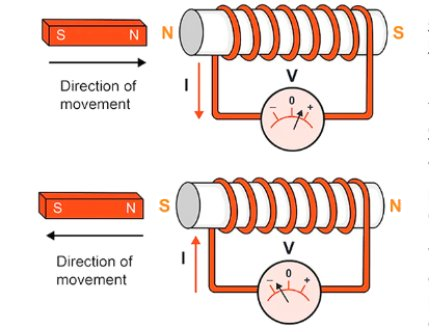
\includegraphics[scale=0.6]{faraday}
    \caption{Ley de inducción de Faraday}
    \label{fig:faraday}
\end{figure}

La corriente debe inducir un campo magnético dentro del solenoide, en la dirección opuesta a la dirección de movimiento del campo magnético inicial. Es de anotar que el mismo efecto se consigue con el imán en reposo y el solenoido entrando y saliendo del imán.

Un motor de un carro eléctrico funciona mediante la interacción entre imanes permanentes y un solenoide. Cuando se deja de acelerar y el carro sigue en movimiento, la rotación de las ruedas hace girar los componentes del motor, generando un campo magnético variable con el tiempo a través del solenoide. Según la Ley de inducción de Faraday, esto induce una corriente eléctrica que recarga la batería. Además, como indica el texto, esta corriente inducida genera su propio campo magnético en una dirección opuesta a la dirección de movimiento; esta oposición al giro actúa como una resistencia física, creando el efecto conocido como \emph{frenado regenerativo}. Ver fig~\ref{fig:ec}

\begin{figure}
    \centering
    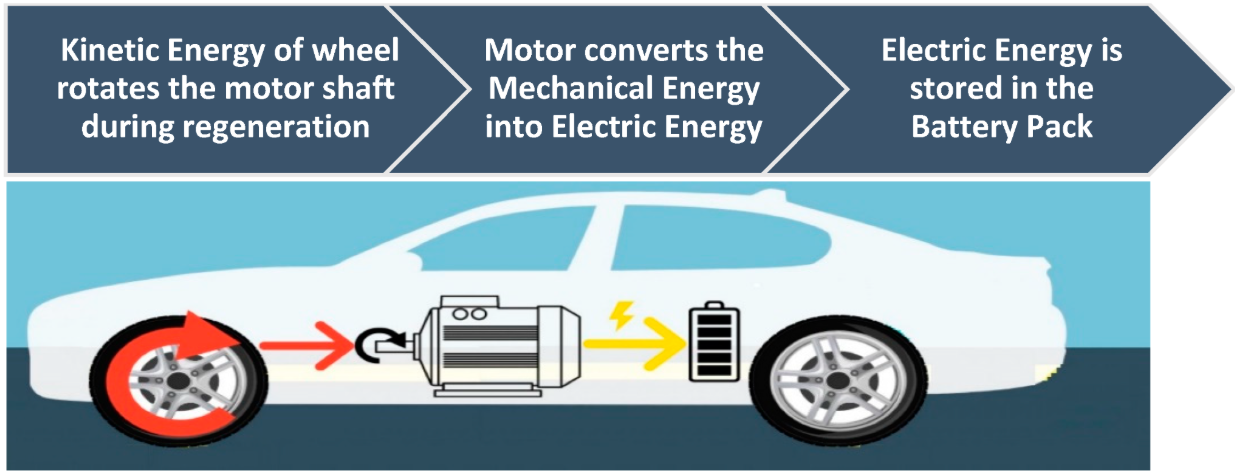
\includegraphics[scale=0.3]{ec}
    \caption{Frenado regenerativo en carro eléctrico. Créditos: \url{
https://doi.org/10.3390/en16145303}}
    \label{fig:ec}
\end{figure}

\subsection{Ejemplo: Estufas de inducción}

A diferencia de una estufa convencional de gas o eléctrica que calienta mediante calor radiante desde una fuente caliente, una estufa de inducción calienta a través de la olla de metal en la que se está cocinando la comida. Una bobina de alambre de cobre se coloca dentro de la encimera. El suministro de electricidad de corriente alterna (CA) produce un campo magnético cambiante en la bobina. Esto induce una corriente  en la olla de metal conductora. La resistencia del metal en la olla, por la que fluye la corriente, transforma la energía eléctrica en calor y cocina la comida.

\section{Electromagnetismo: Ecuaciones de Maxwell}
La contribución final de Maxwell fue la de simetrizar las ecuaciones del electromagnetismo para permitir también que un campo eléctrico que cambie con el tiempo induzca un campo magnético variable con el tiempo. Cómo a su vez un campo magnético variable con el tiempo vuelve a inducir un campo eléctrico variable con el tiempo en un proceso que se repite a la velocidad de la luz. Por consiguiente, la principal predicción de las ecuaciones de Maxwell es la  generación de las ondas electromagnéticas.


\subsection{Ejemplo del Aporte de Maxwell: La Corriente de Desplazamiento}



El aporte crucial de Maxwell, que establece que un campo eléctrico variable induce un campo magnético, se puede ilustrar sin necesidad de cálculo avanzado, analizando simplemente qué sucede cuando cargamos un condensador de placas paralelas.

\begin{figure}
    \centering
    
\begin{tikzpicture}[
    scale=1.2,
    >=Latex,
    % Estilo para el campo magnético (flechas azules curvadas)
    BField/.style={
        draw=blue!80!black, 
        thick, 
        decoration={markings, mark=at position 0.6 with {\arrow{>}}},
        postaction={decorate}
    },
    % Estilo para el campo eléctrico (flechas naranjas)
    EField/.style={
        draw=orange!90!black, 
        thick, 
        ->
    }
]

    % --- 1. EL CIRCUITO EXTERNO ---
    % Coordenadas base
    \coordinate (A) at (0,2);   % Placa izquierda
    \coordinate (B) at (3,2);   % Placa derecha
    \coordinate (TopLeft) at (-2,2);
    \coordinate (BotLeft) at (-2,0);
    \coordinate (BotRight) at (5,0);
    \coordinate (TopRight) at (5,2);

    % Cables y Componentes
    \draw[thick] (A) -- (TopLeft) -- (BotLeft) 
        to[battery1, l=$\mathcal{E}$] (0,0) 
        to[nos, l=Switch] (2,0) -- (BotRight) -- (TopRight) -- (B);

    % Etiqueta de Corriente I (real) en el cable
    \draw[->, thick, red!80!black] (-1.5, 2.2) -- (-0.5, 2.2) node[midway, above] {$I$};
    \draw[->, thick, red!80!black] (3.5, 2.2) -- (4.5, 2.2) node[midway, above] {$I$};

    % --- 2. EL CONDENSADOR (Placas paralelas en perspectiva) ---
    % Placa Izquierda (Anodo +)
    \begin{scope}[shift={(0,2)}, rotate=90]
        \draw[thick, fill=gray!30] (0,0) ellipse (1.5 and 0.2);
        \node at (0.4, 0.4) {\footnotesize $+$}; 
        \node at (-0.4, 0.4) {\footnotesize $+$};
        \node at (0, -0.4) {\footnotesize $+$};
    \end{scope}

    % Placa Derecha (Catodo -)
    \begin{scope}[shift={(3,2)}, rotate=90]
        \draw[thick, fill=gray!30] (0,0) ellipse (1.5 and 0.2);
        \node at (0.4, 0.4) {\footnotesize $-$}; 
        \node at (-0.4, 0.4) {\footnotesize $-$};
        \node at (0, -0.4) {\footnotesize $-$};
    \end{scope}

    % --- 3. EL APORTE DE MAXWELL (En el vacío) ---
    
    % Campo Eléctrico Variable (E) - Flechas Naranjas
    \foreach \y in {2.8, 2.4, 2.0, 1.6, 1.2} {
        \draw[EField] (0.2, \y) -- (2.8, \y);
    }
    \node[orange!90!black, fill=white, inner sep=1pt] at (1.5, 2.5) {$\boldsymbol{E}(t)$ variable};

    % Campo Magnético Inducido (B) - Anillos Azules
    % Representan la "Corriente de Desplazamiento"
    
    % Anillo exterior
    \draw[BField] (1.5, 2) ellipse (0.5 and 1.1);
    \node[blue!80!black, right] at (1.6, 1.0) {$\boldsymbol{B}$ inducido};

    % Anillo interior (para dar efecto 3D)
    \draw[BField, opacity=0.6, thin] (1.5, 2) ellipse (0.25 and 0.55);

    % --- 4. ETIQUETAS EXPLICATIVAS ---
    
    % Etiqueta inferior explicativa
    \node[align=center, font=\small] at (1.5, -1.5) {
        \textbf{Paradoja Resuelta:}\\
        En el vacío no hay cables, pero el cambio
        del campo eléctrico $\boldsymbol{E}$\\ genera un campo
        magnético $\boldsymbol{B}$, cerrando el circuito.
    };

    % Flecha indicando la zona de corriente de desplazamiento
    \draw[<-, thick, gray] (1.5, 0.8) -- (1.5, 0.05) node[below] {Corriente de Desplazamiento ($I_d$)};

\end{tikzpicture}
    \caption{$E(t)$}
    \label{fig:ET}
\end{figure}


\textbf{El Problema de la Corriente Interrumpida:}
Imagina un circuito simple donde una batería carga un condensador. La corriente eléctrica ($I$) fluye por el cable, acumulando cargas en las placas.
\begin{itemize}
    \item Alrededor del cable, sabemos que la corriente genera un campo magnético (Ley de Ampère).
    \item Pero, ¿qué pasa en el espacio vacío entre las placas? Allí no hay cables ni electrones moviéndose ($I=0$). Según la física anterior a Maxwell, el campo magnético debería desaparecer abruptamente en ese espacio.
\end{itemize}
Sin embargo, la naturaleza no funciona así: experimentalmente se detecta un campo magnético entre las placas idéntico al que hay alrededor del cable.

\textbf{La Solución Algebraica:}
Veamos qué está cambiando entre las placas para imitar a una corriente.
Sabemos que el campo eléctrico ($E$) entre dos placas de área $A$ está relacionado con la carga acumulada ($Q$) por la fórmula:
\begin{equation}
    E = \frac{Q}{\epsilon_0 A}
\end{equation}
Si despejamos la carga $Q$, obtenemos:
\begin{equation}
    Q = \epsilon_0 A E
\end{equation}
Sabemos que la corriente eléctrica ($I$) se define como la cantidad de carga que fluye en un tiempo determinado ($t$). Si dividimos la ecuación anterior por el tiempo, recuperamos la corriente:
\begin{equation}
    I = \frac{Q}{t} = \epsilon_0 A \frac{E}{t}
\end{equation}
Aquí está la clave de Maxwell. El término $A \times E$ se conoce como \textbf{Flujo Eléctrico} ($\Phi_E$). Por lo tanto:
\begin{equation}
    I = \epsilon_0 \frac{\Phi_E}{t}
\end{equation}
\textbf{Interpretación Física:}
Aunque no hay electrones cruzando el vacío, el \textbf{cambio del flujo eléctrico en el tiempo} ($\Phi_E / t$) se comporta matemáticamente igual que una corriente.
Maxwell llamó a este término \textbf{Corriente de Desplazamiento}.

\textbf{Conclusión:}
Maxwell corrigió la ley de Ampère estableciendo que el magnetismo tiene dos fuentes posibles:
1. Una corriente eléctrica real (cargas en movimiento).
2. Un campo eléctrico variable (cambio de flujo eléctrico).

Este ``eslabón perdido" permite que un campo eléctrico cambiante cree uno magnético, y viceversa, permitiendo que la energía viaje a través del espacio vacío como una onda electromagnética.




\section{Ondas electromagnéticas}
Es de anotar que así como cargas en movimiento (a velocidad constante) generan un campo magnético, en general cargas aceleradas (velocidad cambiando con el tiempo) generan ondas electromagnéticas. Por lo tanto una partícula cargada negativa orbitando una carga positiva, por ejemplo, pierde constantemente energía por la emisión de ondas electromagnéticas debido a la aceleración por la órbita.



A continuación el espectro de ondas electromagnéticas, ver figura~\ref{fig:em}.

\begin{figure}
    \centering
    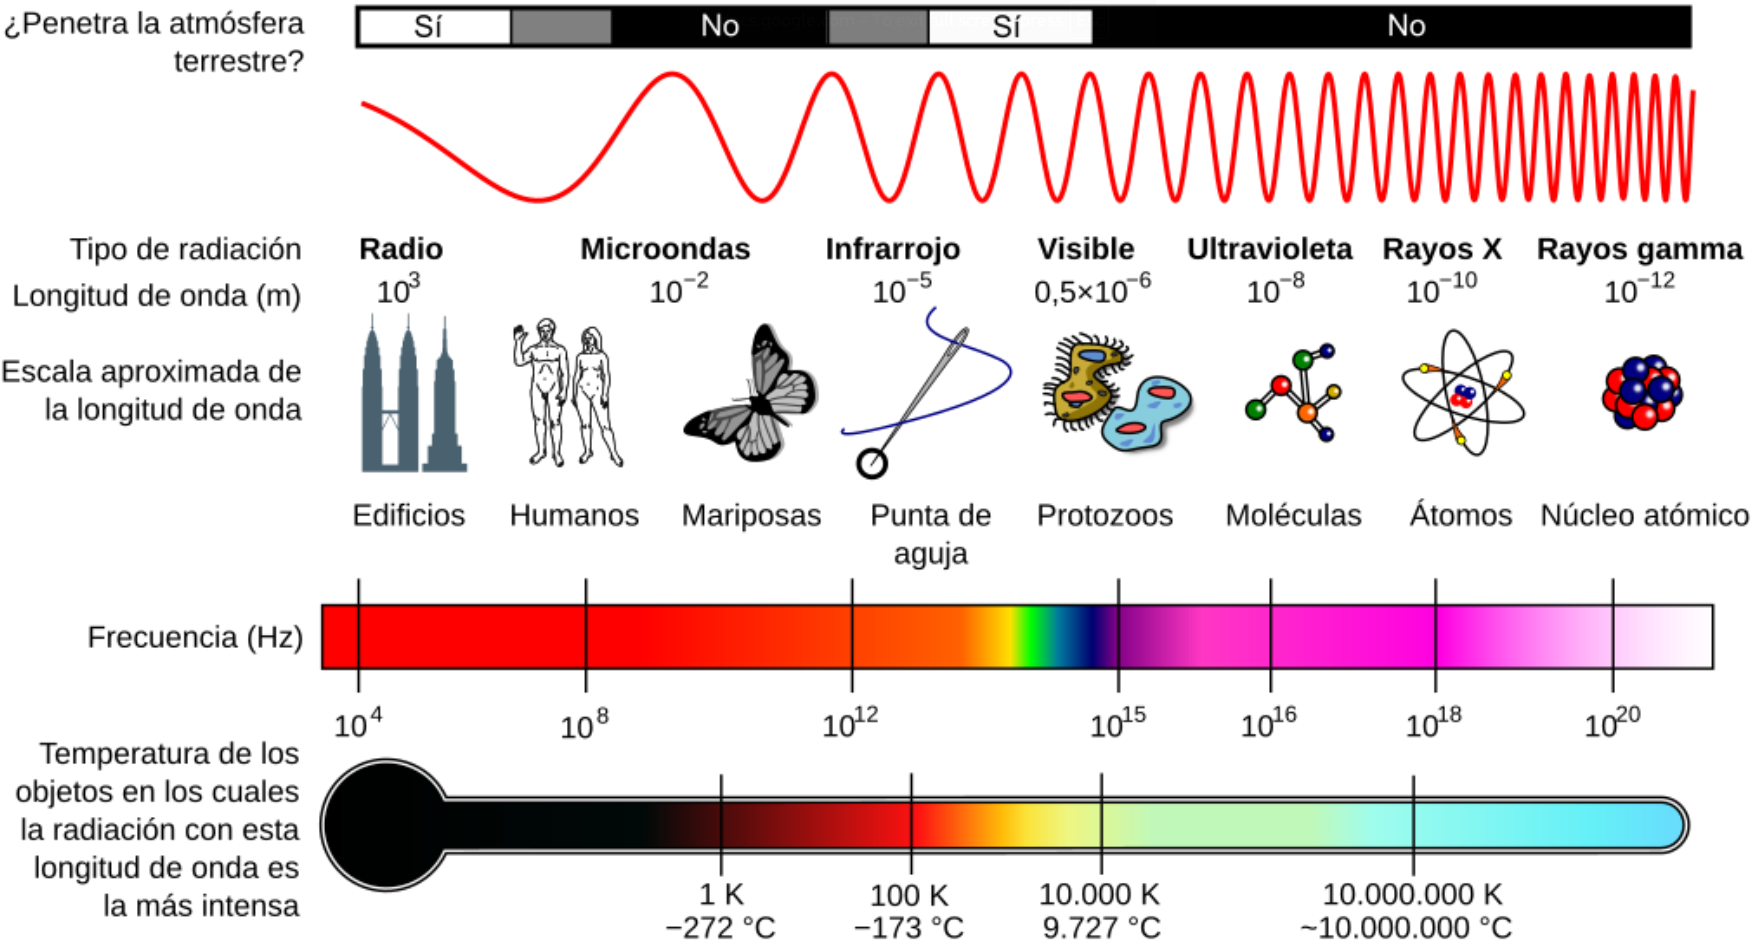
\includegraphics[scale=0.25]{em}
    \caption{Espectro electromagnético}
    \label{fig:em}
\end{figure}


\section{Generación Controlada de Ondas: La Antena}

La predicción fundamental de las ecuaciones de Maxwell es que una carga eléctrica que se acelera debe irradiar energía en forma de ondas electromagnéticas. Para generar estas ondas de manera útil y controlada (como en la radio o el Wi-Fi), no utilizamos descargas aleatorias, sino un dispositivo que mueve las cargas rítmicamente: la \textbf{antena}.

El montaje más sencillo para entender este proceso es la \textbf{antena dipolo} conectada a un generador de corriente alterna (oscilador), como se ilustra en la figura~\ref{fig:antena}

\begin{figure}
    \centering

\begin{tikzpicture}[scale=1.5, >=Latex]

    % Definición de colores consistentes con el texto
    \definecolor{Ecolor}{RGB}{255,140,0} % Naranja para Campo Eléctrico
    \definecolor{Bcolor}{RGB}{0,100,255} % Azul para Campo Magnético

    % --- 1. EL MONTAJE (Antena y Oscilador) ---
    
    % Símbolo del Oscilador (Fuente CA)
    \draw[fill=white, thick] (-1, 0) circle (0.35);
    \node at (-1, 0) {\large $\sim$};
    \node[below, font=\scriptsize, align=center] at (-1, -0.4) {Oscilador\\(Fuente CA)};
    
    % Cables de conexión
    \draw[thick] (-0.65, 0.1) -- (0, 0.1);
    \draw[thick] (-0.65, -0.1) -- (0, -0.1);

    % Varillas de la Antena (Líneas gruesas grises)
    \draw[line width=4pt, gray!60] (0, 0.15) -- (0, 1.8); % Varilla Superior
    \draw[line width=4pt, gray!60] (0, -0.15) -- (0, -1.8); % Varilla Inferior
    
    % Cargas en los extremos (Instántanea en el tiempo)
    \node[circle, fill=red!10, draw=red, inner sep=2pt] at (0, 1.6) {\scriptsize $+$};
    \node[circle, fill=blue!10, draw=blue, inner sep=2pt] at (0, -1.6) {\scriptsize $-$};
    
    % Flechas de Corriente (I)
    \draw[->, thick, black] (-0.3, 0.4) -- (-0.3, 1.0) node[midway, left, font=\footnotesize] {$I(t)$};
    \draw[->, thick, black] (-0.3, -0.4) -- (-0.3, -1.0);

    % --- 2. LOS CAMPOS CERCANOS ---

    % Campo Eléctrico (E) - Arcos naranjas de + a -
    \foreach \angle in {30, 50} {
        % Arcos lado derecho
        \draw[Ecolor, ->, thick] (0, 1.6) to[out=-10-\angle, in=10+\angle] (0, -1.6);
        % Arcos lado izquierdo
        \draw[Ecolor, ->, thick] (0, 1.6) to[out=190+\angle, in=170-\angle] (0, -1.6);
    }
    \node[Ecolor, font=\bfseries] at (0.8, 1.2) {$\boldsymbol{E}$};

    % Campo Magnético (B) - Anillos azules alrededor de la corriente
    % Usamos elipses para dar perspectiva 3D
    \foreach \y in {0.8, -0.8} {
        \draw[Bcolor, thick] (0, \y) ellipse (0.5 and 0.15);
        % Punta de flecha para indicar dirección (Regla mano derecha)
        \draw[Bcolor, ->, thick] (0.01, \y-0.15) -- (0, \y-0.15);
    }
    \node[Bcolor, font=\bfseries] at (0.6, 0.5) {$\boldsymbol{B}$};
    
    % --- 3. LA ONDA VIAJERA (Representación esquemática) ---
    
    \begin{scope}[shift={(2.5,0)}]
        % Eje de propagación
        \draw[->, thick, darkgray] (0,0) -- (3.5,0) node[right, black] {Propagación ($c$)};
        
        % Onda Senoidal para E (Vertical)
        \draw[Ecolor, thick, domain=0:3.2, samples=100] plot (\x, {0.8*sin(\x*360)});
        
        % Vectores E
        \foreach \x in {0.25, 1.25, 2.25} {
            \draw[Ecolor, ->, thick] (\x, 0) -- (\x, 0.8);
        }
        \foreach \x in {0.75, 1.75, 2.75} {
            \draw[Ecolor, ->, thick] (\x, 0) -- (\x, -0.8);
        }
        
        % Vectores B (Horizontal/Perspectiva) - Simulando eje Z saliendo/entrando
        \foreach \x in {0.25, 1.25, 2.25} {
            \draw[Bcolor, ->, thick] (\x, 0) -- (\x-0.3, -0.3); % Saliendo
        }
        \foreach \x in {0.75, 1.75, 2.75} {
            \draw[Bcolor, ->, thick] (\x, 0) -- (\x+0.3, 0.3); % Entrando
        }
        
        % Etiqueta
        \node[above, font=\small, align=center] at (1.5, 1.0) {Onda\\Electromagnética};
    \end{scope}

\end{tikzpicture}

    \caption{Antena}
    \label{fig:antena}
\end{figure}



\subsection{El Mecanismo Físico}

El proceso se puede describir en pasos cíclicos, donde la electricidad se transforma en una onda viajera:

\begin{enumerate}
    \item \textbf{El Oscilador:} Una fuente de voltaje alterno empuja a los electrones hacia arriba y hacia abajo a lo largo de la varilla de metal de la antena. Este movimiento de vaivén implica que las cargas están acelerando y desacelerando constantemente.
    
    \item \textbf{Generación del Campo Eléctrico Variable ($E$):} 
    En un instante, el oscilador acumula cargas positivas en el extremo superior y negativas en el inferior. Esta separación de cargas crea un campo eléctrico alrededor de la antena. Como la polaridad del oscilador cambia continuamente, este campo eléctrico se invierte cíclicamente, creando una perturbación que varía con el tiempo.
    
    \item \textbf{Generación del Campo Magnético Variable ($B$):}
    El movimiento de las cargas para ir de un extremo al otro constituye una corriente eléctrica ($I$). Según la Ley de Ampère, esta corriente genera un campo magnético circular alrededor de la antena. Como la corriente oscila, el campo magnético también varía.
    
    \item \textbf{El Desprendimiento de la Onda:}
    Aquí entra en juego el aporte de Maxwell. Cerca de la antena, los campos $E$ y $B$ están ligados a las cargas. Sin embargo, a medida que los campos cambian, el campo eléctrico variable genera un campo magnético más lejos, y ese nuevo campo magnético genera un campo eléctrico aún más lejos.
    Los campos se ``auto-sostienen" y se desprenden de la antena, viajando por el espacio vacío a la velocidad de la luz.
\end{enumerate}

\subsection{Relación entre Frecuencia y Longitud de Onda}

La onda generada tiene una frecuencia ($f$) determinada por la rapidez con la que oscilan las cargas en la antena. Dado que la onda viaja a una velocidad constante $c$, la distancia entre dos crestas sucesivas de la onda, llamada longitud de onda ($\lambda$), se relaciona algebraicamente mediante:

\begin{equation}
    c = \lambda f
\end{equation}

Donde:
\begin{itemize}
    \item $c \approx 3 \times 10^8$ m/s (Velocidad de la luz).
    \item $\lambda$ es la longitud de onda en metros (m).
    \item $f$ es la frecuencia en Hertz (Hz o $s^{-1}$).
\end{itemize}

\textbf{Ejemplo:} Una emisora de radio FM transmite a una frecuencia de 100 MHz ($100 \times 10^6$ Hz). La longitud de la onda que emite su antena es:

\begin{equation}
    \lambda = \frac{c}{f} = \frac{3 \times 10^8 \, \text{m/s}}{100 \times 10^6 \, \text{s}^{-1}} = 3 \, \text{metros}
\end{equation}

Esto explica por qué las antenas de radio FM deben tener un tamaño del orden de metros para interactuar eficientemente con la onda, mientras que las antenas de los teléfonos móviles (frecuencias de GHz) son de pocos centímetros.

\section{El Colapso del Átomo Clásico: El Límite de la Física Newtoniana}

El modelo planetario del átomo, con un electrón orbitando un protón bajo la fuerza de Coulomb, presenta una contradicción fundamental cuando se combinan las leyes de Newton con el electromagnetismo de Maxwell. A continuación, demostraremos algebraicamente por qué este átomo es inestable y calcularemos su efímera existencia.

\subsection{La Predicción de Maxwell: Pérdida de Energía}

Como vimos en la sección anterior, una carga eléctrica acelerada debe emitir ondas electromagnéticas. Un electrón en órbita circular, aunque tenga rapidez constante, tiene una aceleración centrípeta constante. Por lo tanto, debe perder energía en forma de radiación.

Podemos deducir la fórmula para la potencia radiada ($P$) usando \textbf{análisis dimensional} (álgebra de unidades), sabiendo que la potencia depende de la constante de Coulomb ($k$), la carga ($e$), la aceleración ($a$) y la velocidad de la luz ($c$):

\begin{itemize}
    \item Buscamos unidades de Potencia: $[P] = \text{Newton} \cdot \text{m/s}$.
    \item El término eléctrico es $k e^2$, con unidades $\text{N}\cdot\text{m}^2$.
    \item Para obtener unidades de potencia, necesitamos multiplicar por algo con unidades de $1/(\text{m}\cdot\text{s})$.
    \item Combinando la aceleración ($a$) y la velocidad de la luz ($c$), la única combinación que funciona es $a^2/c^3$.
\end{itemize}

Algebraicamente, esto nos lleva a la \textbf{Fórmula de Larmor} (el factor numérico $2/3$ se obtiene mediante cálculo diferencial e integral):

\begin{equation}
    P = \frac{2}{3} \frac{k e^2 a^2}{c^3}
    \label{eq:larmor}
\end{equation}

\subsection{Estimación Algebraica del Tiempo de Vida}

Para estimar cuánto tiempo tarda el electrón en estrellarse contra el núcleo, podemos usar la relación simple:
\begin{equation}
    \text{Tiempo} (\Delta t) \approx \frac{\text{Energía Total Disponible } (|E|)}{\text{Tasa de Pérdida de Energía } (P)}
\end{equation}

\textbf{Paso 1: Calcular la Aceleración y la Energía Inicial}

Suponemos que el electrón comienza en el radio de Bohr, $r = a_0$. La fuerza de Coulomb proporciona la fuerza centrípeta:
\begin{equation}
    F = m a = \frac{k e^2}{r^2} \implies a = \frac{k e^2}{m r^2}
\end{equation}
Usando la ecuación~\eqref{eq:acentripeta} para la aceleración centrípeta en el movimiento circular
\begin{align*}
    \frac{v^2}{r} = \frac{ke^2}{mr^2}\,,
\end{align*}
tenemos que
\begin{align}
\label{eq:vala2}
    v^2 =\frac{ke^2}{mr}\,.
\end{align}


La energía total ($E$) es la suma de la cinética ($K$) y la potencial ($U$). Usando la ecuación anterior \eqref{eq:vala2}:
\begin{equation}
\label{eq:HE}
    E = K + U = \frac{1}{2}mv^2 - \frac{k e^2}{r} = \frac{k e^2}{2r} - \frac{k e^2}{r} = -\frac{k e^2}{2r}
\end{equation}
La energía disponible para perder (magnitud) es 
\begin{align}
\label{eq:energía}
    |E| = \dfrac{k e^2}{2r}\,.
\end{align}

\textbf{Paso 2: Sustitución en la Fórmula del Tiempo}

Sustituimos la aceleración $a$ en la ecuación de potencia (\ref{eq:larmor}) y luego usamos la fórmula del tiempo:

\begin{equation}
    P = \frac{2 k e^2}{3 c^3} \left( \frac{k e^2}{m r^2} \right)^2 = \frac{2 k^3 e^6}{3 c^3 m^2 r^4}\,.
\end{equation}
%
Ahora dividimos la energía en la ecuación~\eqref{eq:energía} por la potencia obtenida en el paso anterior:
%
\begin{equation}
    \Delta t \approx \frac{|E|}{P} = \frac{\left( \dfrac{k e^2}{2 r} \right)}{\left( \dfrac{2 k^3 e^6}{3 c^3 m^2 r^4} \right)}\,.
\end{equation}
Simplificando la fracción compleja algebraicamente (aplicando extremos y medios):
\begin{equation}
    \Delta t \approx \frac{3c^3m^2r^4ke^2}{4rk^3e^6} \,,
\end{equation}
tenemos finalmente
\begin{equation}
    \Delta t \approx \frac{3 c^3 m^2 r^3}{4 k^2 e^4}\,.
\end{equation}

\textbf{Paso 3: Cálculo Numérico}

Usando las constantes físicas conocidas:
\begin{itemize}
    \item $r \approx 5.3 \times 10^{-11}$ m (Radio de Bohr)
    \item $m \approx 9.11 \times 10^{-31}$ kg (Masa del electrón)
    \item $c \approx 3 \times 10^8$ m/s
    \item $k \approx 9 \times 10^9 \text{ N m}^2/\text{C}^2$
    \item $e \approx 1.6 \times 10^{-19}$ C
\end{itemize}

\begin{equation}
    \Delta t \approx \frac{3 (27 \times 10^{24}) (83 \times 10^{-62}) (149 \times 10^{-33})}{4 (81 \times 10^{18}) (6.5 \times 10^{-76})} \approx 4.7 \times 10^{-11} \text{ s}
\end{equation}

\textbf{Conclusión:}
Bajo las leyes de la física clásica descritas en este texto, el átomo de hidrógeno colapsaría en menos de una diezmilmillonésima de segundo. La estabilidad observada de la materia es la prueba irrefutable de que, a escalas atómicas, las leyes de Newton y Maxwell deben ser reemplazadas por una nueva física: la \textbf{Mecánica Cuántica}.

\section{El Límite de Velocidad Circular: Radiación de Sincrotrón}

La fórmula de Larmor ($P \propto a^2$) tiene una consecuencia drástica para el diseño de aceleradores de partículas. Nos impone un límite práctico a la energía máxima que puede alcanzar un electrón en una órbita circular.

Consideremos un electrón moviéndose en un círculo de radio $R$ con una velocidad $v$ cercana a la de la luz ($v \approx c$).

viene corregida por el factor relativista $\gamma$ como
\begin{equation}    
    P = \frac{2}{3} \frac{k e^2 a^2}{c^3}\gamma^4\,.
    \label{eq:larmor}
\end{equation}
donde $k$: Constante de Coulomb, $e$: carga del electrón, $R$: radio de la órbita, $c$: velocidad de la luz y $\gamma$ es el factor relativista. Ver apéndice~\ref{sec:larmorrel}.

Teniendo en cuenta que el electrón, de masa $m_e$, está acelerado a una energía
\begin{align}
    E = \gamma m_e c^2
\end{align}
y que para una partícula que se mueve en un círculo a la velocidad de la luz 
\begin{equation}
 a = \frac{c^2}{R}\,,   
\end{equation}
donde $R$ es el radio del circulo, calcular la potencia perdida por radiación en el acelerador LEP de $\qty{27}{\kilo\meter}$ de circunferencia. Expresar la respuesta en $\unit{GeV}/\unit{\second}$

\textbf{Solución}
\begin{align*}
    P =  &  \frac{2}{3} \frac{k e^2 c^4}{R^2c^3}\left(\frac{E}{m_ec^2}\right)^4\\
     =  &  \frac{2}{3} \frac{k e^2 c}{R^2}\left(\frac{E}{m_ec^2}\right)^4\\
    =& \frac{A}{R^2} \left(\frac{E}{m_ec^2}\right)^4
\end{align*}
donde
\begin{align}
    m_e c^2 =& \qty{0.511}{MeV}\frac{\unit{GeV}}{\qty{1e3}{MeV}} = \qty{0.511e-3}{GeV}\,.\\
    A =&\frac{2 }{3}  {k e^2 c}=\frac{2}{3}  {\num{8.99e9} (\num{1.602e-19})^2\num{3e8} }\nonumber\\
    =&\qty{4.61e-20}{J\cdot m^2/s}\frac{\unit{GeV}}{\qty{1.602e-10}{J}}=\qty{2.88e-10}{GeV\cdot m^2/s}\,.\\ 
    R =& \frac{\text{circunferencia}}{2\pi} = \frac{\qty{27e3}{m}}{2\pi} = \qty{4297.18}{m}\,
 \end{align}
\begin{align*}
    \frac{A}{R^2} =&\frac{\qty{2.88e-10}{GeV\cdot m^2/s}}{(\qty{4297.18}{m})^2}
     =\qty{1.56e-17}{GeV/s}\,.
\end{align*}
Entonces
\begin{align*}
    P =& \frac{A}{R^2}\left(\frac{E}{m_ec^2}\right)^4\\
    =& \qty{1.56e-17}{GeV/s}\left(\frac{\qty{100}{GeV}}{\qty{0.511e-3}{GeV}}\right)^4\\
    =& \qty{22877}{GeV/s}\,.
\end{align*}
    



Para calcular la energía perdida por radiación en una vuelta, teniendo en cuenta que el electrón se mueve a la velocidad de la luz. Expresaremos la respuesta en $\unit{GeV}$

\textbf{Solución}
\begin{align*}
    \frac{E_{\text{perdida}}}{T} =& P \\
    \frac{E_{\text{perdida}}}{\dfrac{2\pi R}{c}} = & P\\
    \frac{cE_{\text{perdida}}}{2\pi R} = & P\\
    E_{\text{perdida}}  = &\frac{2\pi R}{c} P\\
\end{align*}
Usando la ecuación para $P$
\begin{align*}
    E_{\text{perdida}}  = &\frac{\qty{27e3}{m}}{\qty{3e8}{m/s}}  \qty{22877}{GeV/s}\\
    =&\qty{2.06}{GeV}\,.
\end{align*}

Asumiendo que la energía suministrada a un electrón por vuelta es de $\qty{3.6}{GeV}$ en LEP, podemos calcular la energía máxima a la que se puede acelerar el electrón en dicho acelerador, tal que la energía suministrada para acelerar el electrón durante una vuelta sea igual a la energía perdida por radiación en esa vuelta.

\textbf{Solución}

En este caso
\begin{align*}
    E_{\text{perdida}}  = &\frac{2\pi R}{c} P\\
   E_{\text{perdida}} =&\frac{2\pi R}{c} \frac{2}{3} \frac{k e^2 c}{R^2}\left(\frac{E}{m_ec^2}\right)^4\\
   E_{\text{perdida}} =&\frac{2\pi R}{c} \frac{A}{R^2}\left(\frac{E}{m_ec^2}\right)^4\\
   E_{\text{perdida}} =&\frac{2\pi}{c} \frac{A}{R}\left(\frac{E}{m_ec^2}\right)^4\\
   E_{\text{perdida}} =&C_\gamma \frac{E^4}{R}\\
   \end{align*}
Correspondiente a la ecuación (4.8) de \url{https://inspirehep.net/literature/60854}
donde 
\begin{align}
    C_\gamma =& \frac{2\pi}{c}\frac{A}{\left(m_e c^2\right)^4}\nonumber\\
    =& \frac{2\pi}{\qty{3e8}{m/s}}\frac{\qty{2.88e-10}{GeV\cdot m^2/s}}{(\qty{0.511e-3}{GeV})^4}\\
    =&\qty{8.85e-5}{m\cdot GeV^{-3}}
\end{align}
La energía máxima, $E_{\text{max}}$,  a la que se puede acelerar el electrón es tal que la energía radiada por vuelta, $E_{\text{perdida}}$, sea igual a la energía suministrada por vuelta, $E_{\text{suministrada}}=\qty{3.6}{GeV}$, (ver \url{https://inspirehep.net/literature/560299})

\begin{align*}
    E_{\text{suministrada}} =&C_\gamma \frac{E_{\text{max}}^4}{R}\\
\end{align*}
de donde
\begin{align*}
    E_{\text{max}} =&\left( \frac{R E_{\text{suministrada}} }{C_\gamma}\right)^{1/4}\\
    =&\left(\frac{4297\cdot 3.6}{\num{8.85e-5}}\right)^{1/4}\\
    =&\qty{116}{GeV}
\end{align*}

La energía máxima a la que llegó LEP fue de $\qty{104.5}{GeV}$, $\qty{209}{GeV}$ de energía de centro de masa. Para producir el Higgs se hubiese necesitado una energía de centro de masa de al menos $\qty{220}{GeV}$, que requiere un acelerador de un radio más grande (o acelerando  partículas más pesadas como se verá en el punto siguiente)

\textbf{NOTA:} En \url{https://inspirehep.net/literature/560299} se establece que para LEP, ``the total RF voltage per turn needed is $V =\qty{3630}{MV}$'' que le entrega una energía a un electrón por vuelta de
\begin{align*}
    E_{\text{vuelta}} = e V = e\cdot \qty{3630}{MV} \frac{\unit{eV}}{e}= \qty{3.63}{GeV}
\end{align*}

Sea en adelante, $R_0$, el radio de LEP y $E^0_{\text{suministrada}}$ la energía suministrada por vuelta en LEP. Para una acelerador de radio $R$, la energía suministrada pasa a ser
\begin{align*}
    E_{\text{suministrada}} = E^0_{\text{suministrada}}\frac{R}{R_0}
\end{align*}
Esto es lógico, ya que un túnel más largo permite instalar más cavidades de radiofrecuencia (RF) para acelerar las partículas.

Para el nuevo acelerador de circunferencia de $\qty{100}{km}$
\begin{align*}
    E_{\text{max}} =&\left( \frac{R E_{\text{suministrada}} }{C_\gamma}\right)^{1/4}\\
     =& \left(\frac{R^2 E^0_{\text{suministrada}}}{R_0 C_\gamma}\right)^{1/4}\\
=& \left(\frac{R^2 }{R_0^2}\frac{R_0 E^0_{\text{suministrada}}}{ C_\gamma}\right)^{1/4}\\
=& \left(\frac{R^2 }{R_0^2}\right)^{1/4}\left(\frac{R_0 E^0_{\text{suministrada}}}{ C_\gamma}\right)^{1/4}\\
    =& E^0_{\text{max}}\sqrt{\frac{R}{R_0}}\\
    =& E^0_{\text{max}}\sqrt{\frac{2\pi R}{2\pi R_0}}\\
    =&\qty{116}{GeV}\sqrt{\frac{\qty{100}{km}}{\qty{27}{km}}}\\
    =& \qty{223}{GeV}\,,
\end{align*}
por rayo, para una energía de centro de masa máxima de unos $\qty{440}{\text{GeV}}$\footnote{En \url{https://inspirehep.net/literature/2149705} la dependencia de $E_{\text{max}}$ es con $R^{1/3}$ en lugar de $R^{1/2}$.
}

En el mismo sitio del CERN, donde funciona el LHC y se encontraba LEP, se planea construir un nuevo acelerador de $\qty{90.7}{km}$ llamado el Future Circular Collider (FCC-ee) \url{https://home.cern/science/accelerators/future-circular-collider} que tendrá una energía máxima de centro de masa de $\qty{370}{GeV}$, lo suficiente no sólo para producir el Higgs, sino también pares de top-antitop, cada uno con una masa de $\qty{173}{GeV/c^2}$.

 

Teniendo en cuenta que para un protón se tiene la misma carga, $e^2$, podemos explicar porque el protón se puede acelerar a energías más altas en un acelerador de partículas de la misma circunferencia de $\qty{27}{\kilo\meter}$

\textbf{Solución}
    De
    \begin{align*}
    E_{\text{perdida}} =&\frac{2\pi R}{c} \frac{2}{3} \frac{k e^2 c}{R^2}\left(\frac{E}{m_ec^2}\right)^4\propto \frac{1}{m_e^4}
   \end{align*}
vemos que va con una dependencia inversa con la cuarta potencia de la masa. De modo que a mayor masa (cómo el protón o incluso el muón) menor es la energía perdida por radiación.

La energía perdida por radiación para protones, $E^p_{\text{perdida}}$ es por consiguiente un factor
\begin{align*}
    \left(\frac{m_e}{m_p}\right)^4 =&  \left(\frac{m_e c^2}{m_p c^2}\right)^4\\
    =& \left(\frac{\qty{0.511}{GeV}}{{\qty{0.938}{GeV}}}\right)^4\\
    =&\num{9e-14}
\end{align*}
menor.

\section{Motivación: El Enigma de los Espectros Atómicos}

Tras analizar cómo una antena genera ondas de radio, surge una pregunta natural: si la materia está hecha de cargas eléctricas en movimiento (electrones orbitando núcleos), ¿deberían los átomos comportarse como antenas microscópicas?

Según la física clásica que hemos estudiado hasta ahora, la respuesta es sí. Sin embargo, la naturaleza nos muestra algo totalmente diferente, creando uno de los misterios más grandes que llevó al nacimiento de la mecánica cuántica.

\subsection{El Átomo como una Antena Variable}

Consideremos el modelo clásico del átomo de hidrógeno. El electrón gira alrededor del protón con una frecuencia orbital ($f_{\text{orb}}$).
\begin{itemize}
    \item Al igual que en la antena emisora, esta carga oscilante debería emitir una onda electromagnética (luz) con una frecuencia igual a su frecuencia de rotación: $f_{\text{luz}} = f_{\text{orb}}$.
    \item Como vimos en la sección sobre la inestabilidad, al emitir esta energía, el electrón pierde altura y cae hacia el núcleo.
    \item Al caer a una órbita más pequeña, por conservación de momento angular, el electrón debe girar más rápido. Esto significa que $f_{\text{orb}}$ aumenta continuamente.
\end{itemize}

\textbf{La Predicción Clásica (El ``Grito" de Luz):}
Si la física clásica fuera correcta, un átomo de hidrógeno excitado debería emitir un pulso de luz que cambia suavemente de color, barriendo todas las frecuencias desde el rojo hasta el ultravioleta y más allá, hasta el colapso final. Deberíamos ver un \textbf{espectro continuo} (un arcoíris completo).

\subsection{La Realidad Experimental: Las Líneas Discretas}

Cuando calentamos gas hidrógeno y hacemos pasar su luz a través de un prisma, no vemos un arcoíris. En su lugar, observamos algo sorprendente: el átomo permanece en silencio en la gran mayoría de las frecuencias y solo ``canta'' en colores muy específicos.

Para el hidrógeno visible, solo aparecen cuatro líneas nítidas (la serie de Balmer):
\begin{itemize}
    \item Una línea Roja (656 nm).
    \item Una línea Verde-Azulada (486 nm).
    \item Dos líneas Violetas (434 nm y 410 nm).
\end{itemize}

Esta es la \textbf{huella digital del átomo}. La existencia de estas líneas de emisión implica que el electrón no puede caer en espiral de forma continua. En cambio, debe estar saltando instantáneamente entre ``escalones'' de energía fijos, emitiendo la diferencia exacta de energía como un paquete de luz.

Este comportamiento es imposible de explicar con las ecuaciones de Maxwell y Newton puras. Se necesita una nueva \textbf{regla} que ``congele'' al electrón en órbitas estables y solo permita transiciones específicas: el modelo de Bohr.

\paragraph{La Otra Cara de la Moneda: Las Líneas de Fraunhofer (Espectro de Absorción)}

La evidencia de esta naturaleza cuántica de la materia ya había sido observada, sin saberlo, casi un siglo antes de que se inventara la mecánica cuántica. En 1814, el físico Joseph von Fraunhofer analizó la luz proveniente del Sol utilizando un prisma de alta precisión. Descubrió que el continuo y hermoso arcoíris solar estaba interrumpido por cientos de finas \textbf{líneas oscuras}. 

Estas líneas oscuras son exactamente el fenómeno inverso a la emisión: ocurren por la \textbf{absorción} de la luz. 

El núcleo del Sol emite luz en todas las frecuencias (un espectro continuo). Sin embargo, cuando esta luz atraviesa la atmósfera exterior más fría del Sol, los átomos allí presentes ``roban'' fotones de la luz. Pero debido a la cuantización, los electrones no pueden absorber cualquier energía; \textbf{solo absorben los fotones que tienen la energía exacta necesaria para hacerlos saltar a un nivel superior}. 

El fotón absorbido desaparece del rayo de luz original, dejando una sombra (una línea oscura) en esa frecuencia específica. Las líneas de Fraunhofer son, históricamente, la primera huella digital registrada de la mecánica cuántica, demostrando empíricamente que la materia solo interactúa con la luz en ``paquetes'' o escalones de energía estrictamente definidos.

% --- INSERTAR EN EL PREÁMBULO DEL DOCUMENTO PRINCIPAL (SI NO LO TIENES): ---
% \usepackage{tcolorbox}
% ---------------------------------------------------------------------------

\begin{tcolorbox}[breakable,colback=blue!5!white,colframe=blue!75!black,title=\textbf{Cápsula Histórica: Un Siglo de Magia sin Física}]

Las líneas discretas en los espectros atómicos se fue consolidando como uno de los mayores enigmas en la historia de la ciencia, un problema empírico que tuvo a los físicos en vilo durante exactamente 99 años. 

La crisis no surgió de un día para otro; la comunidad científica pasó por tres etapas fascinantes frente a la ``anomalía'' de las líneas discretas:

\begin{enumerate}
    \item \textbf{El Pragmatismo y la Huella Dactilar (1814 - 1860s):}\\
    Cuando Joseph von Fraunhofer descubrió las líneas oscuras en el espectro del Sol en 1814, los científicos no vieron un fallo en sus teorías, sino una curiosidad. En 1859, Gustav Kirchhoff y Robert Bunsen descubrieron que cada elemento químico ardía con un patrón de líneas único en el laboratorio, y que estas coincidían con las líneas solares. Sin saber \textit{por qué} ocurría, usaron el fenómeno como herramienta. El mayor triunfo de esta fase fue en 1868: al ver líneas solares que no coincidían con nada en la Tierra, descubrieron un elemento extraterrestre nuevo, bautizándolo \textbf{Helio} (del griego \textit{Helios}, Sol).

    \item \textbf{La Numerología de Balmer (1885):}\\
    Al consolidarse el electromagnetismo, la incapacidad de explicar estas líneas causó frustración. Los físicos intentaron modelar el átomo como una cuerda de guitarra vibrando en diferentes ``armónicos'' clásicos, pero fracasaron. Finalmente, Johann Balmer, un profesor de matemáticas y geometría de escuela secundaria, encontró por puro ensayo y error una fórmula algebraica simple que predecía perfectamente las líneas del hidrógeno
    \begin{equation}
        E_n = -\frac{\qty{13.6}{eV}}{n^2}\,.
    \end{equation}
    Sin embargo, nadie sabía \textit{por qué} funcionaba la fórmula de Balmer; era magia matemática sin fundamento físico.

    \item \textbf{La Crisis de Rutherford (1911) y el Triunfo Cuántico:}\\
    El pánico real estalló cuando Ernest Rutherford descubrió la estructura del átomo (un núcleo masivo con electrones orbitando). Como demostramos en este capítulo, al aplicar las impecables leyes de Newton y Maxwell a este modelo, el átomo debería autodestruirse en $10^{-11}$ segundos irradiando un espectro continuo. ¡La existencia misma de la materia era imposible según la física clásica!
\end{enumerate}

No fue hasta 1913 que Niels Bohr, en un acto de atrevimiento intelectual, impuso la cuantización ``a la fuerza'' sobre la mecánica clásica. Al hacerlo y derivar el factor $1/n^2$, le dio por fin a la empírica fórmula de Balmer la base física que le faltó durante casi tres décadas, cerrando la crisis y marcando el nacimiento formal de la \textbf{Mecánica Cuántica}.

\end{tcolorbox}


\section{Modelo de Bohr para el átomo de Hidrógeno}


Para resolver la paradoja de la inestabilidad del átomo, Niels Bohr propuso en 1913 un modelo que mezcla la física clásica con una nueva \textbf{regla} audaz. Bohr asumió que, de alguna manera, existen ciertas órbitas ``especiales'' donde el electrón no irradia energía.

Para encontrar estas órbitas, Bohr introdujo un postulado de \textbf{cuantización}: El momento angular ($L$) del electrón no puede tener cualquier valor, sino solo múltiplos enteros de una constante fundamental.

\subsection{Las Dos Ecuaciones Fundamentales}

Para derivar el modelo, solo necesitamos plantear un sistema de dos ecuaciones algebraicas con dos incógnitas: la velocidad ($v$) y el radio ($r$).

\textbf{1. Equilibrio de Fuerzas (Física Clásica):}
La fuerza eléctrica de atracción debe ser igual a la fuerza centrípeta para mantener la órbita circular. Cómo en la ecuación~\eqref{eq:vala2}
\begin{equation}
    \frac{m v^2}{r} = k \frac{e^2}{r^2} \implies m v^2 = \frac{k e^2}{r}.
    \label{eq:bohr_force}
\end{equation}

\textbf{2. Cuantización del Momento Angular (Nueva Física):}
El momento angular, ecuación~\eqref{eq:Leqmvr}, para una órbita circular,
\begin{align}
  L = mvr\,,
\end{align}
debe ser un múltiplo entero de la constante de Planck reducida ($\hbar = \frac{h}{2\pi}$):
\begin{equation}
    m v r = n \hbar, \quad \text{donde } n = 1, 2, 3, \dots.
    \label{eq:bohr_quant}
\end{equation}

\subsection{Derivación Algebraica del Radio de Bohr}

Nuestro objetivo es encontrar el radio $r$. Tenemos un sistema de ecuaciones.
Primero, despejamos la velocidad $v$ de la ecuación de cuantización (\ref{eq:bohr_quant}):
\begin{equation}
    v = \frac{n \hbar}{m r}.
\end{equation}
Ahora, sustituimos esta expresión de $v$ en la ecuación de fuerzas (\ref{eq:bohr_force}):
\begin{equation}
    m \left( \frac{n \hbar}{m r} \right)^2 = \frac{k e^2}{r}.
\end{equation}
Elevamos al cuadrado y simplificamos,
\begin{equation}
    m \frac{n^2 \hbar^2}{m^2 r^2} = \frac{k e^2}{r},
\end{equation}
lo que se reduce a
\begin{equation}
    \frac{n^2 \hbar^2}{m r^2} = \frac{k e^2}{r}.
\end{equation}
Multiplicamos ambos lados por $r^2$ para despejar el radio, obteniendo
\begin{equation}
    \frac{n^2 \hbar^2}{m} = k e^2 r.
\end{equation}
Finalmente, despejamos $r$. Al depender del número entero $n$, lo llamaremos $r_n$:
\begin{equation}
    r_n = \frac{n^2 \hbar^2}{m k e^2}.
\end{equation}

\textbf{Resultado:} Para el estado fundamental ($n=1$), obtenemos el \textbf{Radio de Bohr ($a_0$)}. Sustituyendo las constantes, recuperamos exactamente el valor que usamos en los problemas anteriores:
\begin{equation}
    a_0 \approx 5.29 \times 10^{-11} \text{ m}.
\end{equation}

\subsection{Derivación de los Niveles de Energía}

Ahora calculamos la energía total permitida para cada órbita.
Como vimos anteriormente en la ecuación~\eqref{eq:HE}, la energía total mecánica es
\begin{equation}
    E = -\frac{1}{2} \frac{k e^2}{r}.
\end{equation}
Sustituimos la expresión que encontramos para el radio $r_n$:
\begin{equation}
    E_n = -\frac{1}{2} k e^2 \left( \frac{1}{r_n} \right) = -\frac{1}{2} k e^2 \left( \frac{m k e^2}{n^2 \hbar^2} \right).
\end{equation}
Agrupando términos, llegamos a
\begin{equation}
    E_n = - \left( \frac{m k^2 e^4}{2 \hbar^2} \right) \frac{1}{n^2}.
\end{equation}

\textbf{Conclusión:}
Todo el término entre paréntesis es una constante. Si calculamos su valor (usando unidades de electronvoltios), obtenemos
\begin{equation}
    E_n = - \frac{13.6 \text{ eV}}{n^2}.
\end{equation}
Esto explica perfectamente el espectro de emisión del hidrógeno: los electrones solo pueden existir en estos niveles de energía discretos y la luz se emite cuando saltan de un nivel $n$ a uno inferior.

\subsubsection{Profundización Conceptual: El Principio de Pauli y la Regla del Octeto}

Al estudiar el átomo, los cursos de química nos enseñan que los átomos buscan tener $8$ electrones en su capa más externa para ser estables, imitando la configuración de un gas noble. Sin embargo, en la física cuántica existe una regla de oro llamada el \textbf{Principio de Exclusión de Pauli}, el cual dicta que \textit{``dos electrones en un mismo átomo no pueden ocupar exactamente el mismo estado cuántico''}. 

A primera vista, esto parece una contradicción flagrante: si no pueden ocupar el mismo estado, ¿cómo es posible amontonar $8$ electrones en el mismo nivel de energía externo sin violar el principio de Pauli?

La respuesta es que el nivel de energía de un átomo (la ``órbita'' de Bohr) no es una única pista donde los electrones se amontonan, sino un conjunto estructurado de ``habitaciones'' con formas geométricas y direcciones diferentes, todas compartiendo aproximadamente la misma energía.

\paragraph{El ``Código Postal'' Cuántico}
Para garantizar que la naturaleza cumpla el Principio de Pauli, basta con que un solo número en el estado cuántico (el ``código postal'' del electrón) sea diferente. Este estado se define por cuatro características (números cuánticos):
\begin{enumerate}
    \item \textbf{Nivel de Energía ($n$):} Es la distancia general al núcleo o ``capa'' principal ($n=1, 2, 3, \dots$).
    \item \textbf{Geometría del Orbital ($l$):} Dentro de ese nivel, hay diferentes formas espaciales. Para acomodar los 8 electrones, nos interesan dos formas: la esférica (llamada orbital $s$) y la lobular (llamada orbital $p$).
    \item \textbf{Orientación Espacial ($m_l$):} Es la dirección hacia donde apunta el orbital en el espacio tridimensional ($x, y, z$).
    \item \textbf{Espín ($m_s$):} Es el giro magnético interno del electrón. Solo tiene dos valores permitidos en el universo: ``arriba'' ($+1/2$) o ``abajo'' ($-1/2$).
\end{enumerate}

\paragraph{Desglosando los 8 Electrones del Gas Noble}
Tomemos como ejemplo el gas Neón, cuyo nivel exterior es el $n=2$. Veamos cómo el álgebra combinatoria permite acomodar exactamente $8$ electrones garantizando que cada uno tenga un estado cuántico único y diferente a los demás:

\begin{itemize}
    \item \textbf{El subnivel $s$ (Geometría esférica):} 
    Solo existe una forma de colocar una esfera en el espacio (no tiene orientación en $x, y, z$). Por lo tanto, hay \textbf{1 solo orbital $s$}.
    \begin{itemize}
        \item Electrón 1: Entra en el orbital $s$ con espín ``arriba''.
        \item Electrón 2: Entra en el orbital $s$ con espín ``abajo''.
    \end{itemize}
    \textit{(Aquí ya tenemos $\mathbf{2}$ electrones. Como agotamos los espines disponibles para esta geometría, el orbital $s$ está lleno).}

    \item \textbf{El subnivel $p$ (Geometría lobular):} 
    Esta geometría nos permite dibujar lóbulos a lo largo de 3 ejes perpendiculares independientes (eje $x$, eje $y$, eje $z$). Es decir, existen \textbf{3 orbitales $p$ distintos}.
    \begin{itemize}
        \item Electrones 3 y 4: Entran en el orbital $p_x$ (uno ``arriba'', uno ``abajo'').
        \item Electrones 5 y 6: Entran en el orbital $p_y$ (uno ``arriba'', uno ``abajo'').
        \item Electrones 7 y 8: Entran en el orbital $p_z$ (uno ``arriba'', uno ``abajo'').
    \end{itemize}
    \textit{(En estas tres orientaciones espaciales caben exactamente $\mathbf{6}$ electrones).}
\end{itemize}

\textbf{Conclusión Física:}
Al sumar matemáticamente los estados disponibles, obtenemos la demostración de la regla química:
\begin{equation}
    2 \text{ (del subnivel } s) + 6 \text{ (del subnivel } p) = \mathbf{8 \text{ electrones distintos}}.
\end{equation}

El misterio queda resuelto. Aunque los $8$ electrones residen en la misma capa externa ($n=2$), \textbf{ningún electrón es idéntico a otro}. Cada uno posee una combinación única de forma geométrica, orientación en el espacio y giro magnético. Cuando un átomo llena su subnivel $s$ y sus tres subniveles $p$, alcanza un estado de simetría esférica perfecta y de mínima energía. Por esta razón, el átomo ya no necesita ceder, ganar ni compartir electrones (enlaces), manifestándose macroscópicamente como un gas noble inerte.

\section{Ejercicios Propuestos del Capítulo 4}

A continuación, se presentan diez ejercicios para poner en práctica los principios del electromagnetismo clásico y su transición hacia la física moderna. Se recomienda repasar las constantes fundamentales (como $k$, $\mu_0$, $\epsilon_0$ y $c$) antes de comenzar.

\begin{enumerate}

    \item 
    \textbf{Ley de Coulomb y Superposición:} Dos cargas puntuales, $q_1 = +4.0  \mu\text{C}$ y $q_2 = +9.0 \mu\text{C}$, están fijas y separadas por una distancia $d = 10 \text{ cm}$. ¿A qué distancia exacta $x$ de la carga $q_1$ debe colocarse una tercera carga $q_3$ (en la línea que las une) para que la fuerza eléctrica neta sobre ella sea exactamente cero ($\sum \boldsymbol{F} = \boldsymbol{0}$)?
    % \textit{[Resp: $x = 4.0 \text{ cm}$].}

    \item \textbf{Energía Potencial Electrostática:} En el núcleo de un átomo de helio existen dos protones (cada uno con carga $e \approx 1.6 \times 10^{-19} \text{ C}$). Si se encuentran separados por una distancia típica nuclear de $r = 2.0 \times 10^{-15} \text{ m}$, calcule la energía potencial electrostática $U_e$ que intenta separarlos. Exprese su resultado primero en Joules y luego conviértalo a Mega-electronvoltios (MeV).
    \textit{[Resp: $U_e \approx 1.15 \times 10^{-13} \text{ J} \approx 0.72 \text{ MeV}$].}

    \item \textbf{Potencia y Consumo de Energía:} Un calentador eléctrico de ambiente se conecta a un enchufe que proporciona un voltaje de $120 \text{ V}$ y extrae una corriente constante de $15 \text{ A}$. 
    \begin{enumerate}
        \item Calcule la potencia eléctrica $P$ consumida por el equipo en Watts.
        \item Si el calentador se deja encendido durante $4 \text{ horas}$ diarias a lo largo de un mes de $30 \text{ días}$, ¿cuál será la energía total consumida en kilovatios-hora (kWh)?
    \end{enumerate}
    \textit{[Resp: a) $P = 1800 \text{ W}$; b) $216 \text{ kWh}$].}

    \item \textbf{Ley de Ampère (Alambre Recto):} Un cable recto de transmisión de alta tensión transporta una inmensa corriente continua de $500 \text{ A}$. Utilice la fórmula algebraica de la Ley de Ampère para calcular la magnitud del campo magnético $B$ que percibe una persona parada en el suelo a $10 \text{ m}$ directamente debajo del cable. Compare este valor con el campo magnético natural de la Tierra (que es de aproximadamente $50 \mu\text{  T}$).
    \textit{[Resp: $B = 10 \mu\text{T}$, que es cinco veces más débil que el campo terrestre].}

    \item \textbf{Diseño de un Solenoide:} Un ingeniero necesita diseñar un electroimán cilíndrico (solenoide) de $L_{\text{bobina}} = 0.5 \text{ m}$ de longitud para generar un campo magnético uniforme de $B = 0.02 \text{ T}$ en su interior. Si el cable disponible solo puede soportar con seguridad una corriente máxima de $I = 5.0 \text{ A}$, ¿cuál es el número mínimo de vueltas o espiras ($N$) que debe enrollar en el cilindro?
    \textit{[Resp: $N \approx 1591 \text{ espiras}$].}

    \item \textbf{Fuerza de Lorentz (Motor Eléctrico):} Un segmento de alambre recto de $L = 0.2 \text{ m}$ de longitud, por el que fluye una corriente de $3.0 \text{ A}$, está situado de forma perpendicular ($\theta = 90^\circ$) dentro del campo magnético uniforme de un motor. Si el alambre experimenta una fuerza magnética lateral de magnitud $|\boldsymbol{F}| = 1.5 \text{ N}$, calcule la intensidad del campo magnético $B$ en el motor.
    \textit{[Resp: $B = 2.5 \text{ T}$].}

    \item \textbf{El Aporte de Maxwell (Corriente de Desplazamiento):} Un condensador de placas paralelas de área $A = 0.1 \text{ m}^2$ se está cargando rápidamente. Aunque no hay electrones cruzando el vacío entre las placas, el campo eléctrico $E$ está aumentando a un ritmo de $\frac{\Delta E}{\Delta t} = 1.0 \times 10^6 \text{ V/(m}\cdot\text{s)}$. Sabiendo que el cambio del flujo eléctrico es $\frac{\Delta \Phi_E}{\Delta t} = A \frac{\Delta E}{\Delta t}$, utilice la ecuación de Maxwell ($I_d = \epsilon_0 \frac{\Delta \Phi_E}{\Delta t}$) para calcular la ``corriente de desplazamiento'' equivalente entre las placas. (Use $\epsilon_0 \approx 8.85 \times 10^{-12} \text{ F/m}$).
    \textit{[Resp: $I_d \approx 8.85 \times 10^{-7} \text{ A}$].}

    \item \textbf{Ondas Electromagnéticas y Antenas:} Un enrutador de red inalámbrica (Wi-Fi) doméstico transmite paquetes de información utilizando ondas electromagnéticas que oscilan a una frecuencia de $2.4 \text{ GHz}$ ($2.4 \times 10^9 \text{ Hz}$). 
    \begin{enumerate}
        \item Calcule la longitud de onda ($\lambda$) de esta señal de radio en centímetros.
        \item En ingeniería de telecomunicaciones, la antena óptima suele medir exactamente un cuarto de la longitud de onda ($\lambda/4$). Según su resultado anterior, ¿cuánto debería medir la antena del enrutador?
    \end{enumerate}
    \textit{[Resp: a) $\lambda = 12.5 \text{ cm}$; b) $3.125 \text{ cm}$].}

    \item \textbf{Radiación de Sincrotrón (Límite Clásico):} En el texto, introdujimos la fórmula de ingeniería para calcular la energía que pierde un electrón ultrarrelativista en cada vuelta de un acelerador debido a su aceleración circular: $\Delta E \approx 8.85 \times 10^{-5} E^4 / R$. Si un colisionador circular tiene un radio de $R = 1000 \text{ m}$ y los electrones viajan con una energía $E = 50 \text{ GeV}$, ¿cuánta energía se pierde en forma de luz en una sola vuelta?
    \textit{[Resp: $\Delta E \approx 0.553 \text{ GeV per vuelta}$].}

    \item \textbf{El Átomo de Bohr (Niveles de Energía Cuantizados):} La solución de Bohr demostró que las energías permitidas para el electrón en el átomo de hidrógeno están dadas por la fórmula algebraica $E_n = -13.6 \text{ eV} / n^2$. 
    Cuando un átomo "canta" y emite su famosa línea roja de luz (llamada línea $H_\alpha$ de la serie de Balmer), el electrón salta de la órbita $n=3$ cayendo a la órbita $n=2$. Calcule la diferencia de energía ($\Delta E = E_3 - E_2$) y demuestre cuál es la energía exacta del fotón rojo emitido.
    \textit{[Resp: $E_3 \approx -1.51 \text{ eV}$, $E_2 = -3.40 \text{ eV}$. El fotón emitido tiene $\Delta E \approx 1.89 \text{ eV}$].}

\end{enumerate}

\appendix


\chapter{Apendices}

\section{Invariancia bajo Rotación de Ejes}

¿Qué ocurre si mantenemos el origen en el mismo lugar, pero rotamos el sistema de coordenadas un ángulo $\theta$?
Como vimos en la Ecuación (1.17), la transformación de las coordenadas individuales al nuevo sistema rotado $S'$ es:
\begin{align}
    x' &= x \cos\theta + y \sin\theta \\
    y' &= -x \sin\theta + y \cos\theta
\end{align}

Determinemos las nuevas componentes del vector diferencia $\Delta\boldsymbol{r}' = (\Delta x', \Delta y')$ en el sistema rotado.
Para la componente $x'$:
\begin{align*}
    \Delta x' &= x'_2 - x'_1 \\
    \Delta x' &= (x_2 \cos\theta + y_2 \sin\theta) - (x_1 \cos\theta + y_1 \sin\theta) \\
    \Delta x' &= (x_2 - x_1) \cos\theta + (y_2 - y_1) \sin\theta \\
    \Delta x' &= \Delta x \cos\theta + \Delta y \sin\theta.
\end{align*}

Haciendo el mismo procedimiento para la componente $y'$:
\begin{align*}
    \Delta y' &= y'_2 - y'_1 \\
    \Delta y' &= (-x_2 \sin\theta + y_2 \cos\theta) - (-x_1 \sin\theta + y_1 \cos\theta) \\
    \Delta y' &= -(x_2 - x_1) \sin\theta + (y_2 - y_1) \cos\theta \\
    \Delta y' &= -\Delta x \sin\theta + \Delta y \cos\theta.
\end{align*}

Nos damos cuenta de que \textbf{las componentes del vector diferencia ($\Delta x, \Delta y$) se transforman exactamente con las mismas ecuaciones geométricas que las coordenadas de posición de un punto individual ($x, y$)}. 

Por lo tanto, la magnitud al cuadrado de este vector diferencia ($|\Delta\boldsymbol{r}'|^2 = (\Delta x')^2 + (\Delta y')^2$) seguirá idénticos pasos algebraicos que en nuestra demostración anterior (donde comprobamos que $(x')^2 + (y')^2 = x^2 + y^2$), y resultará en la misma invarianza fundamental garantizada por la identidad trigonométrica $\sin^2\theta + \cos^2\theta = 1$:
\begin{equation}
    |\Delta\boldsymbol{r}'|^2 = (\Delta x)^2 + (\Delta y)^2 = |\Delta\boldsymbol{r}|^2.
\end{equation}






% --- INICIO DEL APÉNDICE ---
\section{Evidencia Experimental de la Contracción de Lorentz en el LHC}
\label{apendice:contraccion_proton}

A velocidades ultrarrelativistas, las propiedades estructurales de los hadrones sufren transformaciones espaciales severas descritas por la Relatividad Especial. Este apéndice detalla los fundamentos teóricos y las metodologías de medición indirecta de la contracción del diámetro del protón en la dirección del movimiento dentro del Gran Colisionador de Hadrones (LHC).

\subsection{Formulación Matemática y Geometría del Protón Relativista}
En el sistema de referencia del laboratorio, un protón acelerado a una energía de colisión nominal de $E = 6.5\text{ TeV}$ posee un factor de Lorentz ($\gamma$) extremadamente elevado. Sabiendo que la masa en reposo del protón es $m_0 \approx 0.938\text{ GeV/c}^2$, el factor se calcula mediante la relación:

\begin{equation}
\gamma = \frac{E}{m_0 c^2} \approx \frac{6500}{0.938} \approx 6930
\end{equation}

La longitud intrínseca del protón en su sistema de reposo (su diámetro de carga axial) es $L_0 \approx 1.7\text{ fm}$ ($1.7 \times 10^{-15}\text{ m}$). Aplicando la transformación de Lorentz, la longitud contratada $L$ en la dirección del vector velocidad $\vec{v}$ resulta en:

\begin{equation}
L = \frac{L_0}{\gamma} \approx \frac{1.7\text{ fm}}{6930} \approx 2.45 \times 10^{-4}\text{ fm}
\end{equation}

Como consecuencia de esta contracción de casi cuatro órdenes de magnitud, el protón transiciona geométricamente de una distribución de carga esférica a un formalismo de \textit{disco ultraplano} o \textit{pancake relativista}. El diámetro transversal, perpendicular a la dirección del haz, permanece invariante.

\subsection{Manifestaciones Experimentales y Firmas en los Detectores}
Debido a las escalas de longitud subatómicas y la naturaleza cuántica de los constituyentes, la contracción macroscópica no es medible mediante microscopía directa. En su lugar, se verifica de manera inequívoca a través de la física de observables de alta energía:

\begin{itemize}
    \item \textbf{Saturación de Gluones y el Condensado de Vidrio de Color (CGC):} Al comprimirse el volumen del protón a un plano bidimensional, la densidad longitudinal de gluones de bajo momento (pequeño $x$ de Bjorken) diverge exponencialmente. Los experimentos \textbf{ATLAS} y \textbf{CMS} detectan esta saturación mediante la supresión de la producción de partículas a ángulos pequeños (rapideces hacia adelante), un fenómeno predicho únicamente por el modelo de QCD donde los protones se comportan como láminas densas de gluones.
    
    \item \textbf{Sección Eficaz Total de Colisión ($\sigma_{\text{tot}}$):} La probabilidad de interacción en colisiones hadrónicas depende críticamente del perfil de densidad de los proyectiles. Los datos experimentales de dispersión elástica e inelástica demuestran que la sección eficaz escala con el área transversal de choque de dos discos delgados en aproximación de eikonal, divergiendo de los modelos basados en geometrías esféricas o tridimensionales clásicas.
    
    \item \textbf{Anisotropía en el Plasma de Quarks y Gluones (QGP):} En colisiones de iones pesados (p. ej., $\text{Pb-Pb}$ en el detector \textbf{ALICE}), la contracción de Lorentz es tan extrema que la región de superposición de los núcleos en el impacto es prácticamente instantánea en el tiempo del laboratorio. La excentricidad espacial de este volumen bidimensional se transforma, mediante leyes hidrodinámicas de viscosidad casi nula, en un flujo elíptico observable ($v_2$) en la distribución angular de los hadrones resultantes.
\end{itemize}

\subsection{Resumen de Parámetros Cinemáticos}
La Tabla \ref{tab:parametros_lhc} resume las variables cinemáticas del protón bajo las condiciones extremas de operación en el LHC, evidenciando la deformación estructural descrita.

\begin{table}[htbp]
\centering
\caption{Parámetros relativistas del protón en el LHC.}
\label{tab:parametros_lhc}
\vspace{0.2cm}
\begin{tabular}{lcr}
%\toprule
\textbf{Parámetro} & \textbf{Símbolo} & \textbf{Valor Nominal} \\
%\midrule
Energía por haz & $E$ & $6.5 - 7.0\text{ TeV}$ \\
Velocidad relativa & $\beta = v/c$ & $0.999999991$ \\
Factor de Lorentz & $\gamma$ & $\sim 6930$ \\
Diámetro Transversal (Invariante) & $D_{\perp}$ & $\approx 1.7\text{ fm}$ \\
Espesor Longitudinal Contratado & $L$ & $\approx 2.45 \times 10^{-4}\text{ fm}$ \\
%\bottomrule
\end{tabular}
\end{table}




\section{Movimiento Relativista y No Relativista Bajo una Fuerza Constante}
Esta sección proporciona un análisis completo del movimiento de una partícula con velocidad inicial en dos dimensiones bajo la influencia de una fuerza constante en una dirección. Primero derivamos la ecuación de movimiento completamente relativista, luego la expresamos elegantemente en términos de la energía total relativista, revelando su conexión con el Teorema del Trabajo y la Energía. Posteriormente, demostramos el principio de correspondencia mostrando cómo la ecuación relativista se reduce correctamente al caso clásico en el límite no relativista. Finalmente, para completar, derivamos la ecuación de movimiento clásica de forma independiente utilizando el Teorema del Trabajo y la Energía no relativista.

\section{Configuración del Problema}
Consideramos el movimiento de una partícula de masa en reposo $m$.
\begin{itemize}
    \item \textbf{Condiciones Iniciales:} En el tiempo $t=0$, la partícula está en la posición $(x_0, y_0)$ con una velocidad inicial $\boldsymbol{u}_0 = (u_{x0}, u_{y0})$.
    \item \textbf{Fuerza:} Una fuerza constante $\boldsymbol{F}$ actúa solo en la dirección y negativa: $\boldsymbol{F} = (0, -F)$, donde $F$ es una constante positiva.
\end{itemize}
En relatividad, la Segunda Ley de Newton se escribe como la tasa de cambio del momento relativista:
\[ \boldsymbol{F} = \frac{d\boldsymbol{p}}{dt}, \quad \text{donde} \quad \boldsymbol{p} = \gamma m \boldsymbol{u} \]
El factor de Lorentz, $\gamma$, depende de la velocidad total $u = \sqrt{u_x^2 + u_y^2}$:
\[ \gamma = \frac{1}{\sqrt{1 - u^2/c^2}} = \frac{1}{\sqrt{1 - (u_x^2 + u_y^2)/c^2}} \]
Esta dependencia de la velocidad total significa que el movimiento en las direcciones $x$ e $y$ está acoplado, una característica clave de la dinámica relativista.

\section{La Ecuación de Movimiento Relativista}

\section{Resolviendo para el Momento}
La ecuación vectorial $\boldsymbol{F} = d\boldsymbol{p}/dt$ proporciona dos ecuaciones escalares para las componentes del momento $p_x$ y $p_y$.
\begin{itemize}
    \item \textbf{Dirección x:} $F_x = \frac{dp_x}{dt} = 0$. Esto implica que la componente $x$ del momento se conserva:
    \[ p_x(t) = p_{x0} = \gamma_0 m u_{x0} \]
    donde $\gamma_0$ es el factor de Lorentz inicial.
    \item \textbf{Dirección y:} $F_y = \frac{dp_y}{dt} = -F$. Integrando con respecto al tiempo se obtiene:
    \[ p_y(t) = p_{y0} - Ft = \gamma_0 m u_{y0} - Ft \]
\end{itemize}




\section{Encontrando la Velocidad \texorpdfstring{$u_y(t)$}{uy(t)}}
Para encontrar la ecuación de movimiento para $y(t)$, primero necesitamos la velocidad $u_y(t) = dy/dt$. Podemos expresar las componentes de la velocidad en términos del momento y la energía total usando la relación relativista energía-momento $E^2 = (pc)^2 + (mc^2)^2$. Dado que $E=\gamma m c^2$, podemos encontrar $\gamma = \frac{1}{mc}\sqrt{p_x^2 + p_y^2 + m^2c^2}$. Esto conduce a:
\[ u_y(t) = \frac{p_y(t)}{\gamma(t) m} = \frac{c \, p_y(t)}{\sqrt{p_x(t)^2 + p_y(t)^2 + m^2c^2}} \]
Sustituyendo nuestras expresiones dependientes del tiempo para el momento:
\[ \frac{dy}{dt} = u_y(t) = \frac{c (p_{y0} - Ft)}{\sqrt{p_{x0}^2 + (p_{y0} - Ft)^2 + m^2c^2}} \]

\section{Integrando para Encontrar la Posición \texorpdfstring{$y(t)$}{y(t)}}
Integramos la velocidad $u_y(t)$ de $0$ a $t$ para encontrar el desplazamiento.
\[ y(t) - y_0 = \int_0^t \frac{c (p_{y0} - Ft')}{\sqrt{p_{x0}^2 + (p_{y0} - Ft')^2 + m^2c^2}} \, dt' \]
Esta integral se puede resolver usando una sustitución u para el término dentro de la raíz cuadrada. El resultado de la integración es:
\[ y(t) - y_0 = \frac{c}{F} \left( \sqrt{p_{x0}^2 + p_{y0}^2 + m^2c^2} - \sqrt{p_{x0}^2 + (p_{y0} - Ft)^2 + m^2c^2} \right) \]
Esto da la ecuación de movimiento relativista final para la coordenada y.

\section{Teorema del Trabajo y la Energía}

\begin{equation}
dW = \overline{F} \cdot d\overline{s} \label{eq:3}
\end{equation}
es el trabajo infinitesimal realizado por la fuerza $\overline{F}$ mientras la partícula sufre el desplazamiento $d\overline{s}$ a lo largo de su trayectoria. Usamos la segunda ley de Newton del movimiento
\begin{equation}
\overline{F} = \frac{d(m\overline{v})}{dt}
\end{equation}
en la ecuación (\ref{eq:3}) para obtener una expresión para el trabajo infinitesimal
\begin{align*}
dW &= \frac{d(m\overline{v})}{dt} \cdot \overline{v}dt \\
&= \frac{d}{dt}\left(\frac{1}{2}m\overline{v}\cdot\overline{v}\right)dt \\
&= d\left(\frac{1}{2}m\overline{v}^{2}\right).
\end{align*}
Dado que la cantidad escalar $\frac{1}{2}m\overline{v}^{2}$ es la energía cinética de la partícula, se sigue que
\begin{equation}
dW = dT. \label{eq:4}
\end{equation}
La ecuación (\ref{eq:4}) es la forma diferencial del teorema del trabajo y la energía: establece que el trabajo diferencial de la resultante de las fuerzas que actúan sobre una partícula es igual, en cualquier momento, al cambio diferencial en la energía cinética de la partícula. Integrando la ecuación (\ref{eq:4}) entre el punto 1 y el punto 2, correspondientes a las velocidades $\overline{v}_1$ y $\overline{v}_2$ de la partícula, obtenemos
\begin{equation}
W_{12} = \int_{1}^{2} dW = \int_{1}^{2} dT = T_2 - T_1 = \frac{1}{2}m\overline{v}_{2}^{2} - \frac{1}{2}m\overline{v}_{1}^{2}. \label{eq:5}
\end{equation}



\section{Formulación Energética de la Ecuación Relativista}
La ecuación anterior se puede expresar de una forma mucho más elegante y físicamente perspicaz utilizando el concepto de energía total relativista.
Sea $E_0$ la energía total inicial en $t=0$:
\[ E_0 = \sqrt{(p_{x0}^2 + p_{y0}^2)c^2 + (mc^2)^2} \]
Y sea $E(t)$ la energía total en el tiempo $t$:
\[ E(t) = \sqrt{(p_x(t)^2 + p_y(t)^2)c^2 + (mc^2)^2} = \sqrt{(p_{x0}^2 + (p_{y0}-Ft)^2)c^2 + (mc^2)^2} \]
Podemos ver que los términos en nuestra ecuación para $y(t)$ son simplemente $E_0/c$ y $E(t)/c$. Sustituyendo esto se obtiene:
\[ y(t) - y_0 = \frac{c}{F} \left( \frac{E_0}{c} - \frac{E(t)}{c} \right) \]
El factor $c$ se cancela, lo que lleva a la forma notablemente simple:
\[ \boxed{y(t) = y_0 + \frac{E_0 - E(t)}{F}} \]
Esta ecuación es una declaración directa del Teorema del Trabajo y la Energía, $F \Delta y = -\Delta E$, con la energía relativista en lugar de la energía cinética, ver más abajo.

\section{El Límite No Relativista (Principio de Correspondencia)}
Una teoría relativista válida debe reproducir los resultados clásicos a bajas velocidades ($u \ll c$). Mostramos esto usando la aproximación binomial para la energía total $E = \gamma mc^2$. Para velocidades pequeñas, $\gamma \approx 1 + \frac{1}{2}\frac{u^2}{c^2}$, lo que da:
\[ E \approx mc^2 + \frac{1}{2}mu^2 = (\text{Energía en Reposo}) + (\text{Energía Cinética Clásica}) \]
Aplicando esto a nuestra ecuación de movimiento basada en la energía:
\[ y(t) - y_0 = \frac{1}{F} \left[ \left(mc^2 + \frac{1}{2}mu_0^2\right) - \left(mc^2 + \frac{1}{2}mu(t)^2\right) \right] = \frac{m}{2F}(u_0^2 - u(t)^2) \]
En el límite no relativista, las velocidades son $u_x(t) = u_{x0}$ y $u_y(t) = u_{y0} - \frac{F}{m}t$. Sustituyendo esto:
\begin{align*}
y(t) - y_0 &= \frac{m}{2F} \left[ (u_{x0}^2 + u_{y0}^2) - \left(u_{x0}^2 + (u_{y0} - \frac{F}{m}t)^2\right) \right] \\
&= \frac{m}{2F} \left[ u_{y0}^2 - \left(u_{y0}^2 - 2u_{y0}\frac{F}{m}t + \frac{F^2}{m^2}t^2\right) \right] \\
&= \frac{m}{2F} \left[ 2u_{y0}\frac{F}{m}t - \frac{F^2}{m^2}t^2 \right] \\
&= u_{y0}t - \frac{F}{2m}t^2
\end{align*}
Esto produce la ecuación de movimiento clásica final:
\[ \boxed{y(t) = y_0 + u_{y0}t - \frac{F}{2m}t^2} \]
La fórmula relativista se reduce correctamente a la clásica.

\section{Derivación Directa del Caso No Relativista}
Como confirmación final, podemos derivar la ecuación de movimiento clásica directamente del Teorema del Trabajo y la Energía no relativista, $W_{neto} = \Delta K$.
\begin{itemize}
    \item \textbf{Trabajo Realizado:} $W_{neto} = \boldsymbol{F} \cdot \Delta\boldsymbol{r} = -F(y(t) - y_0)$.
    \item \textbf{Cambio en la Energía Cinética:} $\Delta K = K_{final} - K_{inicial} = \frac{1}{2}mu(t)^2 - \frac{1}{2}mu_0^2$.
\end{itemize}
Usando las velocidades clásicas $u_x(t) = u_{x0}$ y $u_y(t) = u_{y0} - \frac{F}{m}t$:
\[ \Delta K = \frac{1}{2}m\left[ (u_{x0}^2 + (u_{y0}-\frac{F}{m}t)^2) - (u_{x0}^2+u_{y0}^2) \right] = \frac{1}{2}m\left[ (u_{y0}-\frac{F}{m}t)^2 - u_{y0}^2 \right] \]
Estableciendo $W_{neto} = \Delta K$:
\[ -F(y(t)-y_0) = \frac{1}{2}m\left[ (u_{y0}^2 - 2u_{y0}\frac{F}{m}t + \frac{F^2}{m^2}t^2) - u_{y0}^2 \right] \]
\[ -F(y(t)-y_0) = -u_{y0}Ft + \frac{F^2}{2m}t^2 \]
Dividiendo por $-F$ se obtiene el resultado idéntico:
\[ y(t) - y_0 = u_{y0}t - \frac{F}{2m}t^2 \]







% --- INFORMACIÓN DEL TÍTULO ---
\section{Derivación de las Transformaciones de Lorentz a partir de Simetrías del Espacio--tiempo}
\label{sec:tl}
\section{El Enfoque de Ignatowski}
Este documento presenta una derivación de las transformaciones de Lorentz basada en principios fundamentales de simetría, en lugar de postular la constancia de la velocidad de la luz. Este enfoque, a veces llamado la derivación de Ignatowski, se basa en el Principio de Relatividad y la homogeneidad e isotropía del espaciotiempo. Mostraremos que estos principios conducen lógicamente a la existencia de una velocidad universal e invariante, que identificamos con la velocidad de la luz.

Ver \cite{Datta:2022cpw} %https://inspirehep.net/literature/2611550


\section{Principios Fundamentales}
La derivación se basa en tres supuestos centrales:
\begin{enumerate}
    \item \textbf{El Principio de Relatividad:} Las leyes de la física son las mismas en todos los sistemas de referencia inerciales.
    \item \textbf{Homogeneidad del Espaciotiempo:} Las leyes de la física son independientes de la posición en el espacio y el tiempo.
    \item \textbf{Isotropía del Espacio:} Las leyes de la física son independientes de la dirección.
\end{enumerate}


\section{Paso 1: Linealidad a partir de la Homogeneidad}
Consideremos dos sistemas de referencia inerciales, $S(x,t)$ y $S'(x',t')$, con $S'$ moviéndose a una velocidad $v$ relativa a $S$ a lo largo del eje x. Buscamos las funciones de transformación $x' = f(x,t)$ y $t' = g(x,t)$.

La homogeneidad del espaciotiempo implica que las ecuaciones de transformación deben ser \textbf{lineales}. Si no lo fueran, un movimiento uniforme en un sistema (una línea recta en un diagrama de espaciotiempo) aparecería como un movimiento acelerado en otro. Esto significaría que las leyes de la física dependerían de la elección del origen, violando la homogeneidad. Por lo tanto, la forma más general de las transformaciones debe ser lineal:
\begin{align*}
x' &= Ax + Bt \\
t' &= Dx + Et
\end{align*}
donde los coeficientes $A, B, D, E$ solo pueden depender de la velocidad relativa, $v$.

\section{Paso 2: Usando Cinemática Básica}
Podemos simplificar los coeficientes usando el movimiento de los orígenes de los sistemas.
\begin{itemize}
    \item El origen del sistema $S'$ ($x'=0$) se mueve con velocidad $v$ en el sistema $S$. Su posición en $S$ es por lo tanto $x=vt$. Sustituyamos esto en nuestra primera ecuación:
    \[ 0 = A(vt) + Bt \implies 0 = (Av+B)t \]
    Esto debe ser válido para todo tiempo $t$, por lo que debemos tener $B = -Av$. La transformación para $x'$ se convierte en:
    \[ x' = Ax - Avt = A(x-vt) \]
\end{itemize}
Renombremos el coeficiente $A(v)$ con la notación más familiar $\gamma(v)$.
\begin{equation} \label{eq:x_prime}
x' = \gamma(v)(x - vt)
\end{equation}

\section{Paso 3: Aplicando la Relatividad y la Isotropía}
El Principio de Relatividad establece que la transformación de $S'$ de vuelta a $S$ debe tener exactamente la misma forma matemática. La única diferencia es que desde la perspectiva de $S'$, el sistema $S$ se mueve con velocidad $-v$. Por lo tanto, la transformación inversa debe ser:
\begin{equation} \label{eq:x}
x = \gamma(-v)(x' + vt')
\end{equation}
Ahora, invocamos la \textbf{isotropía del espacio}. La isotropía significa que la física no debe depender de la dirección del vector velocidad. Por lo tanto, cualquier efecto físico de la transformación solo puede depender de la \textit{rapidez}, $|v|$, no de la dirección de la velocidad. Esto implica:
\[ \gamma(v) = \gamma(-v) \]
Esto simplifica nuestro par de transformaciones a:
\begin{align*}
x' &= \gamma(v)(x - vt) \\
x &= \gamma(v)(x' + vt')
\end{align*}

\section{Paso 4: Encontrando la Transformación del Tiempo}
Todavía necesitamos determinar la transformación para el tiempo. Podemos mostrar que debe tomar la forma simétrica:
\begin{equation} \label{eq:t_prime}
t' = \gamma(v)(t - \alpha(v) x)
\end{equation}
donde $\alpha(v)$ es alguna función de la velocidad. Por el Principio de Relatividad, la transformación inversa debe ser:
\begin{equation} \label{eq:t}
t = \gamma(v)(t' + \alpha(v) x')
\end{equation}
Nótese que la isotropía implica $\alpha(-v) = -\alpha(v)$ (debe ser una función impar).

\section{Paso 5: La Propiedad de Grupo y la Constante Universal}
Este es el paso crucial que reemplaza el postulado de la velocidad de la luz. Consideremos tres sistemas: $S$, $S'$ y $S''$. Sea la velocidad de $S'$ relativa a $S$ $v_1$, y la velocidad de $S''$ relativa a $S'$ $v_2$. La composición de estas dos transformaciones debe dar como resultado una transformación de la misma forma.

Sustituyendo (\ref{eq:x_prime}) y (\ref{eq:t_prime}) en (\ref{eq:x}) y (\ref{eq:t}), podemos resolver para las funciones. Un método más directo es requerir consistencia entre las transformaciones. Sustituyamos (\ref{eq:x_prime}) en (\ref{eq:x}):
\begin{align*}
x &= \gamma(v)(x' + vt') \\
x &= \gamma(v)[\gamma(v)(x-vt) + v t']
\end{align*}
Ahora sustituimos nuestra expresión para $t'$ (\ref{eq:t_prime}):
\begin{align*}
x &= \gamma(v)[\gamma(v)(x-vt) + v \gamma(v)(t - \alpha(v)x)] \\
x &= \gamma(v)^2 [ (x-vt) + v(t-\alpha(v)x) ] \\
x &= \gamma(v)^2 [ x - vt + vt - v\alpha(v)x ] \\
x &= \gamma(v)^2 x (1 - v\alpha(v))
\end{align*}
Como esto debe ser válido para cualquier $x$, debemos tener:
\[ 1 = \gamma(v)^2 (1 - v\alpha(v)) \]
Esto relaciona nuestras dos funciones desconocidas, $\gamma(v)$ y $\alpha(v)$.

A partir del argumento de la propiedad de grupo (considerando tres sistemas), se puede mostrar que la razón $\alpha(v)/v$ debe ser una constante universal, independiente del sistema de referencia. Llamemos a esta constante $K$.
\[ \frac{\alpha(v)}{v} = K \implies \alpha(v) = Kv \]
Ahora sustituimos esto de nuevo en nuestra relación de consistencia:
\[ 1 = \gamma(v)^2 (1 - v(Kv)) = \gamma(v)^2 (1 - K v^2) \]
Resolviendo para $\gamma(v)$:
\[ \boxed{\gamma(v) = \frac{1}{\sqrt{1 - K v^2}}} \]

\section{Paso 6: La Naturaleza Física de la Constante \texorpdfstring{$K$}{K}}
Hemos derivado la forma completa de las transformaciones basándonos únicamente en principios de simetría. La física está contenida en la constante universal $K$.
\begin{enumerate}
    \item \textbf{Caso 1: $K=0$} \\
    Si $K=0$, entonces $\gamma = 1$ y $\alpha=0$. Las transformaciones se convierten en $x' = x - vt$ y $t'=t$. Esta es la \textbf{transformación de Galileo}. En este universo, no hay límite de velocidad.

    \item \textbf{Caso 2: $K<0$} \\
    Si $K$ es negativo, sea $K = -1/R^2$. Entonces $\gamma = 1/\sqrt{1+v^2/R^2}$. Esto corresponde a transformaciones en un espacio euclidiano 4D (rotaciones). Esto es matemáticamente posible pero no describe nuestro universo.

    \item \textbf{Caso 3: $K>0$} \\
    Si $K$ es positivo, debe tener unidades de (1/velocidad$^2$). Definamos una nueva constante $c$ tal que $K = 1/c^2$. Esta constante $c$ debe ser una velocidad universal e invariante. El factor de Lorentz y las transformaciones se convierten en:
    \[ \gamma = \frac{1}{\sqrt{1 - v^2/c^2}} \]
    \[ x' = \gamma(x-vt) \]
    \[ t' = \gamma(t - \frac{v}{c^2}x) \]
    Estas son las \textbf{transformaciones de Lorentz}.
\end{enumerate}

\section{Conclusión}
Sin asumir nunca que la luz viaja a una velocidad constante, hemos demostrado que las simetrías fundamentales del espaciotiempo (homogeneidad e isotropía) y el principio de relatividad conducen a una conclusión sorprendente: \textbf{debe existir una velocidad universal e invariante en nuestro universo}.

Toda la evidencia experimental, desde el electromagnetismo hasta la desintegración de partículas, confirma que vivimos en un universo donde $K > 0$. Llamamos a esta velocidad universal $c$, y la identificamos con la velocidad de la luz en el vacío. La constancia de la velocidad de la luz no es una suposición separada, sino una consecuencia directa de la estructura del espaciotiempo mismo.


\section{Número Imaginario}
Definimos
\begin{align}
    i \equiv \sqrt{-1}\,.
\end{align}
Por lo tanto
\begin{align}
    i^2 = i\cdot i = (-1)^{\frac{1}{2}}(-1)^{\frac{1}{2}}=(-1)^{\frac{1}{2}+\frac{1}{2}}
    =(-1)^{\frac{1+1}{2}}= (-1)^1 = -1\,.
\end{align}
\section{Demostración de la Fórmula de Euler mediante Cálculo}
La fórmula de Euler es
    \begin{align*}
        e^{i\theta} = \cos\theta + i\sin\theta\,.
    \end{align*}

Se puede construir una prueba utilizando cálculo básico.
\begin{enumerate}
    \item Definir una función $f(\theta) = \cos\theta + i\sin\theta$.
    \item Derivar $f(\theta)$ con respecto a $\theta$:
    \[ \frac{df}{d\theta} = -\sin\theta + i\cos\theta \]
    \item Factorizar una $i$ de la derivada, usando $i^2=-1$:
    \[ \frac{df}{d\theta} = i(i\sin\theta + \cos\theta) = i f(\theta) \]
    \item Ahora tenemos una ecuación diferencial simple de primer orden: $\frac{df}{f} = i \, d\theta$.
    \item Integrando ambos lados se obtiene $\ln(f) = i\theta + C$, donde $C$ es la constante de integración.
    \item Exponenciando se obtiene $f(\theta) = e^{i\theta+C} = e^C e^{i\theta}$.
    \item Para encontrar la constante $e^C$, evaluamos la función en $\theta=0$:
    \[ f(0) = \cos(0) + i\sin(0) = 1 + 0 = 1 \]
    De nuestra solución, también tenemos $f(0) = e^C e^{i \cdot 0} = e^C$.
    \item Por lo tanto, la constante $e^C=1$, y nuestra solución final es $f(\theta) = e^{i\theta}$. Como definimos $f(\theta) = \cos\theta + i\sin\theta$, la identidad queda demostrada:
    \begin{align}
    \boxed{
        e^{i\theta} = \cos\theta + i\sin\theta\,.
        }
    \end{align}
\end{enumerate}

\section{Derivando Seno y Coseno de la Fórmula de Euler}
Una aplicación poderosa de la fórmula de Euler es expresar el seno y el coseno en términos de exponenciales complejas. Esto se logra tratando la fórmula de Euler y su conjugada como un sistema de dos ecuaciones lineales.

\section{El Sistema de Ecuaciones}
Comenzamos con la fórmula de Euler y una segunda versión donde $\theta$ es reemplazado por $-\theta$:
\begin{align*}
    e^{i\theta} &= \cos\theta + i\sin\theta \tag{A.1} \\
    e^{-i\theta} &= \cos(-\theta) + i\sin(-\theta) = \cos\theta - i\sin\theta \tag{A.2}
\end{align*}
La segunda ecuación utiliza la propiedad par del coseno ($\cos(-\theta)=\cos\theta$) y la propiedad impar del seno ($\sin(-\theta)=-\sin\theta$).

\section{Resolviendo para \texorpdfstring{$\cos\theta$}{cos(theta)}}
Para aislar $\cos\theta$, sumamos las ecuaciones (A.1) y (A.2) para eliminar los términos del seno:
\begin{align*}
    e^{i\theta} + e^{-i\theta} &= (\cos\theta + i\sin\theta) + (\cos\theta - i\sin\theta) \\
    e^{i\theta} + e^{-i\theta} &= 2\cos\theta
\end{align*}
Resolviendo para $\cos\theta$ se obtiene:
\[ \boxed{\cos\theta = \frac{e^{i\theta} + e^{-i\theta}}{2}} \]

\section{Resolviendo para \texorpdfstring{$\sin\theta$}{sin(theta)}}
Para aislar $\sin\theta$, restamos la ecuación (A.2) de la ecuación (A.1) para eliminar los términos del coseno:
\begin{align*}
    e^{i\theta} - e^{-i\theta} &= (\cos\theta + i\sin\theta) - (\cos\theta - i\sin\theta) \\
    e^{i\theta} - e^{-i\theta} &= 2i\sin\theta
\end{align*}
Resolviendo para $\sin\theta$ se obtiene:
\[ \boxed{\sin\theta = \frac{e^{i\theta} - e^{-i\theta}}{2i}} \]
Estas definiciones son fundamentales en muchas áreas de la física y la ingeniería, particularmente en el análisis de Fourier.

\section{Conexión con las Funciones Hiperbólicas}

Estas formas exponenciales son sorprendentemente similares a las definiciones de las funciones hiperbólicas:
\[ \cosh(x) = \frac{e^x + e^{-x}}{2} \quad \text{y} \quad \sinh(x) = \frac{e^x - e^{-x}}{2} \]
Por comparación directa, podemos ver la relación formal utilizada en el texto principal para la rotación de Wick.
\begin{itemize}
    \item Comparando $\cos\theta$ con $\cosh(x)$, vemos que si establecemos $x=i\theta$, obtenemos $\cosh(i\theta) = \frac{e^{i\theta} + e^{-i\theta}}{2} = \cos\theta$.
    \item Comparando $\sin\theta$ con $\sinh(x)$, vemos que $\sinh(i\theta) = \frac{e^{i\theta} - e^{-i\theta}}{2} = i \left( \frac{e^{i\theta} - e^{-i\theta}}{2i} \right) = i\sin\theta$.
\end{itemize}
Esto demuestra la profunda consistencia matemática entre las funciones trigonométricas e hiperbólicas en el plano complejo.

\section{La Matriz de Lorentz}
Podemos escribir la transformación $X' = \Lambda X$ como:
\[ \begin{pmatrix} t' \\ x'  \end{pmatrix} = \Lambda \begin{pmatrix} t \\ x  \end{pmatrix} \]
Inspeccionando las ecuaciones de transformación, podemos escribir la matriz $\Lambda$ primero en términos de $\gamma$ y $v$, y luego sustituir las funciones hiperbólicas:
\[
\Lambda(\xi) = \begin{pmatrix} \gamma & -v\gamma  \\ -v\gamma & \gamma  \\  \end{pmatrix}
=
\boxed{
\begin{pmatrix} \cosh\xi & -\sinh\xi  \\ -\sinh\xi & \cosh\xi  \\  \end{pmatrix}
}
\]
Esto revela que un impulso de Lorentz es una \textbf{rotación hiperbólica} en el espaciotiempo.

\section{La Rotación de Wick: Impulsos como Rotaciones Imaginarias}

La conexión con la geometría se vuelve aún más sorprendente si tratamos la rapidez como un ángulo imaginario. Este procedimiento es parte de una técnica conocida como \textbf{rotación de Wick}.

\section{De Funciones Hiperbólicas a Trigonométricas}
Establezcamos la rapidez $\xi$ como un ángulo imaginario, $\xi = i\theta$. Usando las definiciones de las funciones hiperbólicas en términos de exponenciales, encontramos las siguientes identidades:
\begin{align*}
    \cosh(i\theta) &= \frac{e^{i\theta} + e^{-i\theta}}{2} = \cos\theta \\
    \sinh(i\theta) &= \frac{e^{i\theta} - e^{-i\theta}}{2} = i \left( \frac{e^{i\theta} - e^{-i\theta}}{2i} \right) = i\sin\theta
\end{align*}

\section{La Transformación Completa en el Espaciotiempo Euclidiano}
Ahora, realicemos una rotación de Wick completa aplicando dos cambios simultáneamente:
\begin{enumerate}
    \item \textbf{Rapidez Imaginaria:} $\xi \to i\theta$
    \item \textbf{Tiempo Imaginario:} $t \to i\tau$ (y por lo tanto $t' \to i\tau'$)
\end{enumerate}
Aplicamos esto a la ecuación matricial $X'=\Lambda X$, centrándonos en las componentes $(t,x)$:
\[ \begin{pmatrix} i\tau' \\ x' \end{pmatrix} = \begin{pmatrix} \cos\theta & -i\sin\theta \\ -i\sin\theta & \cos\theta \end{pmatrix} \begin{pmatrix} i\tau \\ x \end{pmatrix} \]
Multiplicando esto se obtienen dos ecuaciones:
\begin{align*}
    i\tau' &= (\cos\theta)(i\tau) + (-i\sin\theta)(x) = i(\tau\cos\theta - x\sin\theta) \\
    x' &= (-i\sin\theta)(i\tau) + (\cos\theta)(x) = (-i^2)\tau\sin\theta + x\cos\theta = \tau\sin\theta + x\cos\theta
\end{align*}
Después de cancelar la $i$ de la primera ecuación, obtenemos el resultado final:
\[
\begin{aligned}
\tau' &= \tau\cos\theta - x\sin\theta \\
x' &= x\cos\theta + \tau\sin\theta
\end{aligned}
\]
Esto es precisamente una rotación euclidiana estándar en el plano $(\tau, x)$. En forma matricial:
\[
\boxed{
\begin{pmatrix} \tau' \\ x' \end{pmatrix} = \begin{pmatrix} \cos\theta & -\sin\theta \\ \sin\theta & \cos\theta \end{pmatrix} \begin{pmatrix} \tau \\ x \end{pmatrix}
}
\]

% --- TABLA AÑADIDA INICIO ---
\begin{table}[h!]
\centering
\caption{Resumen de la Rotación de Wick: Mapeo de un Impulso de Lorentz a una Rotación Euclidiana.}
\label{tab:wick}
\begin{tabular}{l|l|l}
\hline
\textbf{Característica} & \textbf{Espaciotiempo de Minkowski (Impulso)} & \textbf{Espaciotiempo Euclidiano (Rotación)} \\
\hline \hline
Coordenadas & $(t, x)$ & $(\tau, x)$, donde $t = i\tau$ \\
\hline
Intervalo Invariante & $s^2 = t^2 - x^2$ & $d^2 = \tau^2 + x^2$ \\
\hline
Tipo de Transformación & Rotación Hiperbólica & Rotación Circular \\
\hline
Parámetro & Rapidez, $\xi = \tanh^{-1}(v)$ & Ángulo, $\theta$ (donde $\xi = i\theta$) \\
\hline
Forma Matricial & $\begin{pmatrix} \cosh\xi & -\sinh\xi \\ -\sinh\xi & \cosh\xi \end{pmatrix}$ & $\begin{pmatrix} \cos\theta & -\sin\theta \\ \sin\theta & \cos\theta \end{pmatrix}$ \\
\hline
Interpretación Física & Cambio de velocidad & Rotación geométrica formal \\
\hline
\end{tabular}
\end{table}
% --- TABLA AÑADIDA FIN ---

\section{Producto escalar en forma matricial (rotación)}
Sea 
\begin{align*}
    X =& \begin{pmatrix}
        x\\  
        y
    \end{pmatrix},&
    X^{\operatorname{T}} =& 
    \begin{pmatrix}
        x&y\\
    \end{pmatrix},&
\end{align*}
y
\begin{align*}
    \delta = \begin{pmatrix}
        1 & 0\\
        0 & 1\\
    \end{pmatrix}.
\end{align*}
Podemos definir el producto escalar como
\begin{align*}
    X^{\operatorname{T}}\cdot X 
   \equiv & X^{\operatorname{T}}\cdot \delta \cdot X \\
   = &\begin{pmatrix}
        x&y\\
    \end{pmatrix}\cdot  \begin{pmatrix}
        1 & 0\\
        0 & 1\\
    \end{pmatrix} \cdot \begin{pmatrix}
        x\\  
        y
    \end{pmatrix} \\
   = &\begin{pmatrix}
        x&y\\
    \end{pmatrix}\cdot \begin{pmatrix}
        x\\  
        y
    \end{pmatrix} \\
= & x^2 +y ^2\,.
\end{align*}

\newpage
\section{Producto escalar en forma matricial (impulso)}
Sea 
\begin{align*}
    X =& \begin{pmatrix}
        t\\  
        x
    \end{pmatrix},&
    X^{\operatorname{T}} =& 
    \begin{pmatrix}
        t&x\\
    \end{pmatrix},&
\end{align*}
y
\begin{align*}
    g = \begin{pmatrix}
        1 & 0\\
        0 & -1\\
    \end{pmatrix}.
\end{align*}
Podemos definir el producto escalar como
\begin{align*}
    X^{\operatorname{T}}\cdot X 
   \equiv & X^{\operatorname{T}}\cdot g \cdot X \\
   = &\begin{pmatrix}
        t&x\\
    \end{pmatrix}\cdot  \begin{pmatrix}
        1 & 0\\
        0 & -1\\
    \end{pmatrix} \cdot \begin{pmatrix}
        t\\  
        x
    \end{pmatrix} \\
   = &\begin{pmatrix}
        t&x\\
    \end{pmatrix}\cdot \begin{pmatrix}
        t\\  
        -x
    \end{pmatrix} \\
= & t^2 - x ^2\,.
\end{align*}



% --- DOCUMENT END ---

\begin{align*}
    Q =&\begin{pmatrix}
      \color{Green}  u\\
       \color{red} d
    \end{pmatrix} \hspace{1cm}
    L= \begin{pmatrix}
      \color{Green}  \nu\\
       \color{red} e
    \end{pmatrix}
\end{align*}


\begin{align*}
m_\mu \gg& m_e\\
    L_e =&\begin{pmatrix}
      \color{Green}  \nu_e\\
       \color{red} e
    \end{pmatrix} \hspace{1cm}
    L_\mu= \begin{pmatrix}
      \color{Green}  \nu_\mu\\
       \color{red} \mu
    \end{pmatrix}
\end{align*}

\begin{align*}
    \partial_\mu = \left(\frac{\partial}{c\partial t},
    \frac{\partial}{\partial x},
    \frac{\partial}{\partial y},
    \frac{\partial}{\partial z}\right)
\end{align*}
\hspace{5cm}Producto escalar de Lorentz
\begin{align*}
    \partial_\mu\cdot \partial_\mu V =& 0\\ 
    \frac{\partial^2 V}{c^2\partial t^2}-
    \frac{\partial^2 V}{\partial x^2}-
    \frac{\partial^2 V}{\partial y^2}-
    \frac{\partial^2 V}{\partial z^2} =& 0\,.
\end{align*}

\newpage
\def\mipa{11cm}
\begin{minipage}{\mipa}
La magnitud de la fuerza que la corriente $I_1$ ejerce sobre una carga $q_2$ que fluye con la corriente $I_2$ a una velocidad $\boldsymbol{v}$, para recorrer la distancia $L$ en un tiempo $t$, es
\end{minipage}

\begin{align*}
F_2 =& q_2 v B_1\\
=& q_2\frac{L}{t} B_1\\
=& \frac{q_2}{t} L B_1\\
=& I_2 L B_1\,.
\end{align*}

\begin{minipage}{\mipa}
Reemplazando la magnitud del campo magnético 
a una distancia $r$ del alambre con corriente $I_1$ (donde se encuentra el alambre con corriente $I_2$) dado por
\end{minipage}

\begin{align*}
    B_1 = \frac{\mu_0 I_1}{2\pi r}\,,
\end{align*}

\begin{minipage}{\mipa}
tenemos que la magnitud fuerza por unidad de longitud que ejerce $I_1$ sobre $I_2$ es
\end{minipage}

\begin{align*}
    \frac{F_2}{L} = \frac{\mu_0 I_1 I_2}{2\pi r}\,,
\end{align*}

\begin{minipage}{\mipa}
en la dirección hacia el cable con corriente $I_1$, como se muestra en la figura.
\end{minipage}


% --- Inicio del código LaTeX para insertar ---

\section*{Derivación de las Transformaciones de Lorentz usando las dos ecuaciones}

\section*{Introducción}

Las transformaciones de Lorentz son el conjunto de ecuaciones que relacionan las coordenadas de espacio y tiempo de un evento, medidas por dos observadores en diferentes sistemas de referencia inerciales. La derivación se basa en los dos postulados fundamentales de la Relatividad Especial:
\begin{enumerate}
    \item \textbf{El Principio de Relatividad:} Las leyes de la física son las mismas en todos los sistemas de referencia inerciales.
    \item \textbf{La Constancia de la Velocidad de la Luz:} La velocidad de la luz en el vacío, $c$, es la misma para todos los observadores inerciales.
\end{enumerate}

\section*{Configuración Inicial}
Consideramos dos sistemas de referencia inerciales, $S(x,t)$ y $S'(x',t')$. El sistema $S'$ se mueve con una velocidad constante $v$ relativa a $S$ a lo largo del eje x. En $t=t'=0$, sus orígenes coinciden. Nuestro objetivo es encontrar las funciones que conectan sus coordenadas.

\section*{Paso 1: La Suposición de Linealidad}
Debido a la homogeneidad del espaciotiempo, las ecuaciones de transformación deben ser lineales. Por lo tanto, podemos escribir las formas más generales:
\begin{align*}
    x' &= Ax + Bt \\
    t' &= Dx + Et
\end{align*}
donde los coeficientes $A, B, D, E$ solo pueden depender de la velocidad relativa $v$. Las coordenadas perpendiculares al movimiento no se ven afectadas ($y'=y$, $z'=z$).

\section*{Paso 2: Encontrar los Coeficientes para \texorpdfstring{$x'$}{x'}}
Consideramos el origen del sistema $S'$ ($x'=0$), que se mueve con velocidad $v$ en el sistema $S$, por lo que su posición es $x=vt$. Sustituyendo en la primera ecuación:
\[ 0 = A(vt) + Bt \implies 0 = (Av + B)t \]
Como esto debe ser cierto para todo tiempo $t$, se deduce que $B = -Av$. Sustituyendo de nuevo en la ecuación para $x'$:
\[ x' = Ax - Avt = A(x-vt) \]
Renombramos la constante $A(v)$ con el símbolo convencional $\gamma(v)$, el factor de Lorentz:
\begin{equation} \label{eq:x_prime_trans}
    \boxed{x' = \gamma(v)(x - vt)}
\end{equation}

\section*{Paso 3: Encontrar los Coeficientes \texorpdfstring{$D$}{D} y \texorpdfstring{$E$}{E} para \texorpdfstring{$t'$}{t'}}
Ahora aplicamos el segundo postulado. Imaginemos que en $t=t'=0$ se emite un pulso de luz desde el origen común.

\subsection*{Caso 1: Pulso de luz hacia la derecha (+x)}
En $S$, el frente de luz se describe por $x = ct$. En $S'$, por $x' = ct'$. Sustituimos estas condiciones en nuestras ecuaciones de transformación:
\begin{itemize}
    \item De la ecuación para $x'$: $ct' = \gamma(ct - vt) \implies t' = \gamma t (1 - v/c)$.
    \item De la ecuación para $t'$: $t' = D(ct) + Et = t(Dc + E)$.
\end{itemize}
Igualando ambas expresiones para $t'$ (el factor $t$ se cancela):
\begin{equation} \label{eq:sys1}
    \gamma (1 - v/c) = Dc + E
\end{equation}

\subsection*{Caso 2: Pulso de luz hacia la izquierda (-x)}
En $S$, el frente de luz es $x = -ct$. En $S'$, es $x' = -ct'$. Sustituimos de nuevo:
\begin{itemize}
    \item De la ecuación para $x'$: $-ct' = \gamma(-ct - vt) \implies t' = \gamma t (1 + v/c)$.
    \item De la ecuación para $t'$: $t' = D(-ct) + Et = t(E - Dc)$.
\end{itemize}
Igualando las expresiones para $t'$:
\begin{equation} \label{eq:sys2}
    \gamma (1 + v/c) = E - Dc
\end{equation}

Ahora tenemos un sistema de dos ecuaciones lineales para las incógnitas $D$ y $E$:
\[ \begin{cases} E + Dc = \gamma (1 - v/c) \\ E - Dc = \gamma (1 + v/c) \end{cases} \]
\textbf{Para encontrar E}, sumamos las dos ecuaciones:
\[ (E + Dc) + (E - Dc) = \gamma (1 - v/c) + \gamma (1 + v/c) \implies 2E = 2\gamma \implies \boxed{E = \gamma(v)} \]
\textbf{Para encontrar D}, restamos la segunda ecuación de la primera:
\[ (E + Dc) - (E - Dc) = \gamma (1 - v/c) - \gamma (1 + v/c) \implies 2Dc = \gamma(-2v/c) \implies \boxed{D = -\frac{\gamma(v) v}{c^2}} \]

\section*{Paso 4: Formular la Transformación del Tiempo y Encontrar \texorpdfstring{$\gamma(v)$}{gamma(v)}}
Con los coeficientes $D$ y $E$, la transformación para $t'$ es:
\[ t' = Dx + Et \implies t' = -\frac{\gamma v}{c^2}x + \gamma t \]
Reordenando, obtenemos la forma familiar:
\begin{equation} \label{eq:t_prime_trans}
    \boxed{t' = \gamma \left(t - \frac{vx}{c^2}\right)}
\end{equation}
Para encontrar la forma explícita de $\gamma(v)$, usamos el Principio de Relatividad. La transformación inversa de (\ref{eq:t_prime_trans}) es $t = \gamma(t' + vx'/c^2)$. Sustituimos en ella las expresiones para $x'$ y $t'$ que hemos encontrado:
\begin{align*}
    t &= \gamma \left[ \gamma \left(t - \frac{vx}{c^2}\right) + \frac{v}{c^2} \gamma(x - vt) \right] \\
    t &= \gamma^2 \left[ t - \frac{vx}{c^2} + \frac{vx}{c^2} - \frac{v^2t}{c^2} \right] \\
    t &= \gamma^2 \left[ t - \frac{v^2t}{c^2} \right] = \gamma^2 t \left(1 - \frac{v^2}{c^2}\right)
\end{align*}
Cancelando $t$ de ambos lados, nos queda $1 = \gamma^2 (1 - v^2/c^2)$. Finalmente, resolvemos para $\gamma(v)$:
\[ \gamma^2 = \frac{1}{1 - v^2/c^2} \implies \boxed{\gamma = \frac{1}{\sqrt{1 - v^2/c^2}}} \]

\section*{Resumen de las Transformaciones de Lorentz}
Habiendo encontrado todos los coeficientes y la forma de $\gamma$, tenemos el conjunto completo de las transformaciones de Lorentz:
\[
\boxed{
\begin{aligned}
t' &= \gamma \left( t - \frac{vx}{c^2} \right) \\
x' &= \gamma (x - vt) \\
y' &= y \\
z' &= z
\end{aligned}
\quad \text{con} \quad
\gamma = \frac{1}{\sqrt{1 - v^2/c^2}}
}
\]

% --- Inicio del código LaTeX para insertar ---

\section{Derivación del Factor 3/5 para la Energía Potencial de una Esfera}
\label{sec:3_5}

El factor numérico de $3/5$ en la fórmula para la energía potencial electrostática de una esfera cargada no es arbitrario; es el resultado de un cálculo riguroso utilizando integración para encontrar la energía total necesaria para ensamblar dicha esfera.

\section{El Concepto: Energía de Ensamblaje}

See \url{https://www.macmillanlearning.com/studentresources/college/physics/tiplermodernphysics6e/classial_concept_review/chapter_11_ccr_20_electrostatic_energy_of_a_sphere_of_charge.pdf}

La energía potencial total del núcleo se puede conceptualizar como el \textbf{trabajo total} que una fuerza externa debe realizar para construir la esfera de carga, trayendo pequeñas cantidades de carga (infinitesimales, $dq$) desde el infinito y añadiéndolas capa por capa contra la repulsión electrostática de la carga ya acumulada. La energía total es la suma (la integral) de todo el trabajo infinitesimal realizado en cada paso.

\section{La Derivación (usando Cálculo)}

\paragraph{Paso 1: Configurar el Problema.}
Queremos construir una esfera de radio final $R$ y carga total $Q$. Asumimos que la carga se distribuye uniformemente, por lo que la densidad de carga $\rho$ es constante:
\begin{equation}
    \rho = \frac{\text{Carga Total}}{\text{Volumen Total}} = \frac{Q}{\frac{4}{3}\pi R^3}\,.
\end{equation}
En un paso intermedio del proceso, hemos construido una esfera de radio $r$ (con $r < R$).

\paragraph{Paso 2: Calcular la Carga y el Potencial de la Esfera Intermedia.}
La carga acumulada en la esfera de radio $r$, denotada como $q(r)$, es:
\begin{equation}
    q(r) = \rho \cdot V(r) = \left( \frac{Q}{\frac{4}{3}\pi R^3} \right) \cdot \left( \frac{4}{3}\pi r^3 \right) = Q \frac{r^3}{R^3}\,.
\end{equation}
El potencial eléctrico en la superficie de esta esfera, $V(r)$, debido a la carga $q(r)$ es:
\begin{equation}
    V(r) = k \frac{q(r)}{r} = k \frac{1}{r} \left( Q \frac{r^3}{R^3} \right) = k \frac{Q r^2}{R^3}\,.
\end{equation}

\paragraph{Paso 3: Calcular el Trabajo para Añadir la Siguiente Capa.}
Ahora, traemos una capa esférica infinitesimalmente delgada de carga, $dq$, desde el infinito. El grosor de esta capa es $dr$, y su carga es $dq = \rho \cdot (4\pi r^2 dr)$. El trabajo infinitesimal ($dU$) necesario para traer esta carga $dq$ al potencial $V(r)$ es:
\begin{equation}
    dU = V(r) \cdot dq\,.
\end{equation}
Sustituimos nuestras expresiones para $V(r)$ y $dq$:
\[
    dU = \left( k \frac{Q r^2}{R^3} \right) \cdot \left( \rho (4\pi r^2 dr) \right)\,.
\]

\paragraph{Paso 4: Sustituir la Densidad y Simplificar.}
Reemplazamos la expresión para la densidad $\rho$:
\begin{align*}
    dU &= \left( k \frac{Q r^2}{R^3} \right) \cdot \left( \frac{Q}{\frac{4}{3}\pi R^3} \cdot 4\pi r^2 dr \right)\,, \\
       &= k \frac{Q^2 r^4}{R^6} \cdot 3 \cdot dr\,, \\
       &= 3k \frac{Q^2}{R^6} r^4 dr\,.
\end{align*}

\paragraph{Paso 5: Integrar para Encontrar la Energía Total.}
La energía potencial total, $U_e$, es la integral de todo el trabajo infinitesimal $dU$ necesario para construir la esfera desde un radio 0 hasta el radio final $R$:
\begin{align*}
    U_e &= \int_0^R dU = \int_0^R 3k \frac{Q^2}{R^6} r^4 dr\,, \\
        &= 3k \frac{Q^2}{R^6} \int_0^R r^4 dr\,, \\
        &= 3k \frac{Q^2}{R^6} \left[ \frac{r^5}{5} \right]_0^R\,, \\
        &= 3k \frac{Q^2}{R^6} \left( \frac{R^5}{5} - 0 \right)\,, \\
        &= \frac{3}{5} k \frac{Q^2 R^5}{R^6} = \frac{3}{5} k \frac{Q^2}{R}\,.
\end{align*}

\section*{Conclusión}
Hemos demostrado que la energía potencial electrostática total (o energía de autointeracción) de una esfera con carga $Q$ y radio $R$, distribuida uniformemente, es:
\begin{equation}
    \boxed{
    U_e = \frac{3}{5} k \frac{Q^2}{R}
    }\,.
\end{equation}
El factor $3/5$ es, por tanto, un coeficiente puramente geométrico que surge de la integración sobre el volumen de una esfera bajo la suposición de densidad de carga uniforme.

% --- Fin del código LaTeX ---
% --- Fin del código LaTeX ---




\section{Ejemplo: contenido de positrones del Universo}
La estimación del orden de magnitud para el número total de \textbf{positrones} en el universo observable es altamente especulativa debido a su naturaleza fugaz. Sin embargo, al contrastarlos con el contenido de materia dominante, se puede llegar a una estimación aproximada.


El orden de magnitud más razonable para el número de positrones en el universo observable se encuentra probablemente en el rango de $\mathbf{10^{65}}$ a $\mathbf{10^{70}}$.

\subsection*{Base de la Estimación}

Esta estimación no se obtiene directamente de un único experimento de flujo como el \text{AMS-02}, sino que se deriva del desequilibrio establecido entre materia y antimateria, y de la tasa de aniquilación en nuestra galaxia.

\subsection*{1. Comparación con la Materia ($\approx 10^{80}$)}

El número total de \textbf{electrones} y \textbf{protones} (materia ordinaria) en el universo observable se estima en alrededor de $\mathbf{10^{80}}$.

Dado que todo el universo observable está compuesto casi en su totalidad por materia (y no por antimateria), el número total de positrones debe ser \textbf{mucho menor} que la cifra de $10^{80}$ de electrones.

\subsection*{2. Producción y Aniquilación de Positrones}

Los positrones se producen continuamente por eventos de alta energía y desintegración radiactiva, pero son destruidos muy rápidamente por \textbf{aniquilación} con electrones. Por lo tanto, su número está determinado por un equilibrio de producción-aniquilación en lugar de ser un remanente cosmológico.

\begin{itemize}
    \item \textbf{Producción Galáctica de Positrones:} Las observaciones de la línea $\mathbf{511 \text{ keV } \gamma}$ en el Centro Galáctico, que es una firma de la aniquilación electrón-positrón, sugieren que los positrones se producen en la Vía Láctea a una tasa de aproximadamente $\mathbf{10^{42}}$ positrones por segundo ($\dot{N}_{e^+} \approx 10^{42} \text{ s}^{-1}$).
    \item \textbf{Número en Estado Estacionario en la Vía Láctea:} Para mantener esta tasa de producción, se estima que el número total de positrones que flotan actualmente en el fondo difuso de la Vía Láctea es de $\mathbf{N_{e^+} \approx 10^{56}}$ a $\mathbf{10^{57}}$.
\end{itemize}

\subsection*{3. Escala al Universo}

Para escalar esto al universo observable, multiplicamos la estimación Galáctica por el número estimado de galaxias. Se estima que el universo observable contiene entre $10^{11}$ y $10^{12}$ galaxias.

La estimación resultante es:
$$N_{\text{Positrones, Universo}} \approx N_{\text{Positrones, Galaxia}} \times N_{\text{Galaxias}}$$
$$N_{\text{Positrones, Universo}} \approx 10^{56} \text{ a } 10^{57} \times 10^{11} \text{ a } 10^{12}$$
$$N_{\text{Positrones, Universo}} \approx 10^{67} \text{ a } 10^{69}$$

Este cálculo aproximado sugiere un orden de magnitud de $\mathbf{10^{68}}$.

\begin{table}[h!]
    \centering
    \begin{tabular}{|l|c|}
        \hline
        \textbf{Partícula} & \textbf{Orden de Magnitud (Universo Observable)} \\
        \hline
        Electrones y Protones (Materia) & $\approx 10^{80}$ \\
        \hline
        Fotones y Neutrinos & $\approx 10^{89}$ \\
        \hline
        \textbf{Positrones (Antimateria)} & $\approx 10^{65} - 10^{70}$ \\
        \hline
    \end{tabular}
    \caption{Estimación del Orden de Magnitud de Partículas}
\end{table}

\section{Derivación Algebraica de la Fórmula de Larmor Relativista}
\label{sec:larmorrel}

En la física clásica, la potencia $P$ (energía radiada por unidad de tiempo) de una carga acelerada está dada por la fórmula de Larmor, que depende del cuadrado de la aceleración: $P \propto a^2$. Sin embargo, cuando un electrón se mueve a velocidades cercanas a la de la luz en un acelerador circular (sincrotrón), esta fórmula debe corregirse por efectos relativistas. 

A continuación, demostraremos algebraicamente cómo surge esta corrección sin utilizar cálculo diferencial, analizando cómo se transforman el espacio, el tiempo y la velocidad entre dos observadores.

\subsubsection{Configuración de los Sistemas de Referencia}

Imaginemos un electrón moviéndose en una órbita circular. En un instante dado, alineamos nuestro sistema de coordenadas de modo que el electrón se mueve a lo largo del eje $x$ con velocidad $v$, y su aceleración centrípeta apunta hacia el eje $y$.

Definimos dos sistemas inerciales:
\begin{itemize}
    \item \textbf{Sistema del Laboratorio ($S$):} El observador estacionario ve al electrón moverse con velocidad horizontal $\boldsymbol{u}_x = v$ y experimentar un cambio de velocidad vertical $\Delta \boldsymbol{u}_y$ durante un pequeño intervalo de tiempo $\Delta t$. Su aceleración medida es $a = \frac{\Delta \boldsymbol{u}_y}{\Delta t}$.
    \item \textbf{Sistema Propio ($S'$):} Una nave imaginaria que viaja a velocidad constante $v$ junto al electrón. En este instante, el electrón está en reposo respecto a la nave ($\boldsymbol{u}'_x = 0$). La aceleración que experimenta el electrón en su propio sistema es la \textbf{aceleración propia} $a' = \frac{\Delta \boldsymbol{u}'_y}{\Delta t'}$.
\end{itemize}

Nuestro objetivo es encontrar algebraicamente la relación entre $a'$ y $a$.

\subsubsection{Paso 1: Transformación del Intervalo de Tiempo ($\Delta t'$)}

Primero, necesitamos saber cuánto tiempo transcurre en el sistema propio ($S'$) en comparación con el laboratorio ($S$). Utilizamos la ecuación de transformación de Lorentz para intervalos de tiempo:
\begin{equation}
    \Delta t' = \gamma \left( \Delta t - \frac{v \Delta x}{c^2} \right).
\end{equation}
Como estamos observando a la partícula, la distancia $\Delta x$ que recorre en el laboratorio durante el tiempo $\Delta t$ es simplemente $\Delta x = v \Delta t$. Sustituyendo esto en la ecuación obtenemos
\begin{equation}
    \Delta t' = \gamma \left( \Delta t - \frac{v (v \Delta t)}{c^2} \right).
\end{equation}
Factorizamos el intervalo de tiempo $\Delta t$:
\begin{equation}
    \Delta t' = \gamma \Delta t \left( 1 - \frac{v^2}{c^2} \right).
\end{equation}
Sabemos por definición que el término entre paréntesis es exactamente el inverso del factor de Lorentz al cuadrado, es decir, $\left(1 - \frac{v^2}{c^2}\right) = \frac{1}{\gamma^2}$. Al sustituirlo, la ecuación se simplifica a
\begin{equation}
    \Delta t' = \gamma \Delta t \left( \frac{1}{\gamma^2} \right) = \frac{\Delta t}{\gamma}.
    \label{eq:delta_t_algebraico}
\end{equation}
\textit{(Nota: Esto es simplemente la dilatación del tiempo: el tiempo propio $\Delta t'$ es más corto que el tiempo del laboratorio $\Delta t$ por un factor $\gamma$).}

\subsubsection{Paso 2: Transformación de la Velocidad Transversal ($\Delta \boldsymbol{u}'_y$)}

Ahora debemos analizar el cambio de velocidad en la dirección perpendicular ($y$). La fórmula relativista para transformar velocidades en el eje transversal es:
\begin{equation}
    \boldsymbol{u}'_y = \frac{\boldsymbol{u}_y}{\gamma \left( 1 - \frac{v \boldsymbol{u}_x}{c^2} \right)}.
\end{equation}
En nuestro experimento, la velocidad inicial en $y$ es cero. Luego de un pequeño instante, el electrón adquiere una velocidad vertical $\Delta \boldsymbol{u}_y$. En ese mismo instante, su velocidad horizontal sigue siendo prácticamente la misma, $\boldsymbol{u}_x = v$ (ya que en un movimiento circular el cambio en la rapidez tangencial es nulo).

Sustituimos la componente horizontal $\boldsymbol{u}_x = v$ en el denominador:
\begin{equation}
    \Delta \boldsymbol{u}'_y = \frac{\Delta \boldsymbol{u}_y}{\gamma \left( 1 - \frac{v(v)}{c^2} \right)} = \frac{\Delta \boldsymbol{u}_y}{\gamma \left( 1 - \frac{v^2}{c^2} \right)}.
\end{equation}
Nuevamente, utilizamos la identidad mágica $\left(1 - \frac{v^2}{c^2}\right) = \frac{1}{\gamma^2}$:
\begin{equation}
    \Delta \boldsymbol{u}'_y = \frac{\Delta \boldsymbol{u}_y}{\gamma \left( \frac{1}{\gamma^2} \right)}.
\end{equation}
Al simplificar el denominador ($\gamma / \gamma^2 = 1/\gamma$), la fracción se invierte, dándonos el resultado:
\begin{equation}
    \Delta \boldsymbol{u}'_y = \gamma \Delta \boldsymbol{u}_y.
    \label{eq:delta_v_algebraico}
\end{equation}
Físicamente, esto significa que, debido a la relatividad del espaciotiempo, el observador que viaja con la partícula percibe un "empujón" lateral $\gamma$ veces más violento que el observador estacionario.

\subsubsection{Paso 3: La Aceleración Propia ($a'$)}

La aceleración propia que verdaderamente experimenta el electrón se define como su cambio de velocidad dividido por su propio intervalo de tiempo. Utilizando las Ecuaciones (\ref{eq:delta_v_algebraico}) y (\ref{eq:delta_t_algebraico}), obtenemos
\begin{equation}
    a' = \frac{\Delta \boldsymbol{u}'_y}{\Delta t'} = \frac{\gamma \Delta \boldsymbol{u}_y}{\left( \frac{\Delta t}{\gamma} \right)}.
\end{equation}
Aplicando las reglas del álgebra para dividir fracciones (extremos y medios), multiplicamos por $\gamma$:
\begin{equation}
    a' = \gamma \cdot \gamma \left( \frac{\Delta \boldsymbol{u}_y}{\Delta t} \right).
\end{equation}
Reconociendo que la fracción final es simplemente la aceleración medida en el laboratorio ($a = \Delta \boldsymbol{u}_y / \Delta t$), llegamos a nuestra conclusión geométrica:
\begin{equation}
    a' = \gamma^2 a.
    \label{eq:aceleracion_propia}
\end{equation}

\subsubsection{Paso 4: La Fórmula de Larmor para el Sincrotrón}

Para una partícula cargada, la \textbf{potencia total radiada} ($P = \Delta E / \Delta t$) es un invariante relativista, lo que significa que el laboratorio y la partícula acuerdan en el mismo valor de potencia ($P = P'$). 

En el sistema propio de la partícula, la velocidad es cero, por lo que las leyes de la física clásica aplican perfectamente. La potencia clásica de Larmor depende del cuadrado de la aceleración:
\begin{equation}
    P = \frac{2}{3} \frac{k e^2}{c^3} (a')^2.
\end{equation}
Para predecir qué observaremos desde la Tierra, debemos escribir esta ecuación en términos de la aceleración del laboratorio ($a$). Al sustituir la Ecuación (\ref{eq:aceleracion_propia}), obtenemos
\begin{equation}
    P = \frac{2}{3} \frac{k e^2}{c^3} (\gamma^2 a)^2.
\end{equation}
Al elevar el paréntesis al cuadrado, descubrimos la fórmula final para la radiación de sincrotrón:
\begin{equation}
    P = \frac{2}{3} \frac{k e^2 a^2}{c^3} \gamma^4.
\end{equation}

\textbf{Conclusión:} 
El factor $\gamma^4$ no es un ajuste arbitrario; es la consecuencia ineludible de aplicar álgebra básica a las transformaciones de Lorentz. Dado que el reloj de la partícula corre más lento (factor $\gamma$) y su cambio de velocidad lateral se magnifica (otro factor $\gamma$), la aceleración que siente es $\gamma^2$ veces mayor. Como la radiación de energía requiere cuadrar esa aceleración, el efecto total estalla proporcionalmente a $\gamma^4$, poniendo un límite infranqueable a la energía que podemos darle a un electrón en un acelerador circular.

\section{Ejercicios resueltos}

\noindent
\textbf{\ref{sec:ejerciciosrelatividad}}
\begin{itemize}
    \item[Ejercicio \ref{item:starshot}:] 

    \textbf{Solución:}

\textit{a) Tiempo medido desde la Tierra.} Con $\beta = v/c = 0.2$, el factor de
Lorentz es
\begin{equation}
    \gamma = \frac{1}{\sqrt{1-\beta^2}} = \frac{1}{\sqrt{1-(0.2)^2}} \approx 1.0206\,.
\end{equation}
El tiempo en el marco terrestre es simplemente la distancia propia dividida entre
la velocidad:
\begin{equation}
    t_{\text{Tierra}} = \frac{D_0}{v} = \frac{4.3\ \text{años luz}}{0.2c} = 21.5\ \text{años}\,.
\end{equation}

\textit{b) Tiempo propio de la bacteria.} Por dilatación del tiempo, el reloj
biológico de la bacteria —en reposo respecto a la sonda— mide un tiempo propio
menor:
\begin{equation}
    \tau = \frac{t_{\text{Tierra}}}{\gamma} \approx \frac{21.5\ \text{años}}{1.0206}
    \approx 21.07\ \text{años}\,.
\end{equation}

\textit{c) Longitud contraída percibida.} Para la bacteria, la distancia a Alfa
Centauri no es la propia $D_0$; está contraída en la dirección del movimiento por
el mismo factor $\gamma$:
\begin{equation}
    L' = \frac{D_0}{\gamma} \approx \frac{4.3\ \text{años luz}}{1.0206}
    \approx 4.213\ \text{años luz}\,.
\end{equation}

\textit{d) Verificación de consistencia.} Si la bacteria recorre la distancia ya
contraída $L'$ a la velocidad $v$, el tiempo propio que debería transcurrir es
simplemente $L'/v$:
\begin{equation}
    \tau' = \frac{L'}{v} \approx \frac{4.213\ \text{años luz}}{0.2c} \approx 21.07\ \text{años}\,.
\end{equation}
Como $\tau' = \tau$, confirmamos que la dilatación del tiempo y la contracción de
la longitud no son dos efectos independientes, sino dos maneras equivalentes de
describir exactamente el mismo fenómeno físico —consistentes entre sí con
precisión matemática exacta, incluso para un organismo microscópico atrapado en
un chip del tamaño de un sello postal.


\item[Ejercicio \ref{item:redshift}:]

\textbf{Solución Detallada:}
    \begin{enumerate}
        \item[a)] Despejamos la longitud de onda observada de la definición del \textit{redshift}:
        \begin{equation}
            \lambda_{\text{obs}} = (1 + z) \lambda_0.
        \end{equation}
        Sustituyendo $z = 14$ y $\lambda_0 = 121.6 \text{ nm}$:
        \begin{equation}
            \lambda_{\text{obs}} = (1 + 14)(121.6 \text{ nm}) = 15(121.6 \text{ nm}) = 1824 \text{ nm}.
        \end{equation}
        Convirtiendo a micrómetros ($1 \text{ $\mu$m} = 1000 \text{ nm}$):
        \begin{equation}
            \lambda_{\text{obs}} = \frac{1824}{1000} \text{ $\mu$ m} = 1.824 \text{ $\mu$ m}.
        \end{equation}
        
        \item[b)] Aplicamos la relación de onda para hallar la frecuencia observada ($f_{\text{obs}}$):
        \begin{equation}
            f_{\text{obs}} = \frac{c}{\lambda_{\text{obs}}} = \frac{3.0 \times 10^8 \text{ m/s}}{1.824 \times 10^{-6} \text{ m}} \approx 1.64 \times 10^{14} \text{ Hz} = 164 \text{ THz}.
        \end{equation}
        Esta frecuencia se ubica plenamente en la región del \textbf{Infrarrojo Cercano}, lo que justifica por qué los instrumentos del telescopio James Webb debieron optimizarse específicamente para capturar esta radiación.
        
        \item[c)] Igualamos la ecuación del \textit{redshift} con la fórmula del Efecto Doppler Relativista de alejamiento (Ecuación \eqref{eq:doppler_aleja}):
        \begin{equation}
            1 + z = \sqrt{\frac{1 - \frac{v}{c}}{1 + \frac{v}{c}}}.
        \end{equation}
        Elevamos ambos lados al cuadrado:
        \begin{equation}
            (1 + z)^2 = \frac{1 - \frac{v}{c}}{1 + \frac{v}{c}}.
        \end{equation}
        Hacemos el cambio algebraico temporal $u = v/c$:
        \begin{equation}
            (1 + z)^2 (1 + u) = 1 - u \implies (1 + z)^2 + (1 + z)^2 u = 1 - u.
        \end{equation}
        Agrupamos los términos con $u$ a un lado:
        \begin{equation}
            (1 + z)^2 - 1 = u \left[ 1 + (1 + z)^2 \right].
        \end{equation}
        Despejando $u$ ($v/c$), obtenemos la identidad solicitada:
        \begin{equation}
            \frac{v}{c} = \frac{(1 + z)^2 - 1}{(1 + z)^2 + 1}.
        \end{equation}
        
        \item[d)] Sustituimos $z = 14$ en la fórmula obtenida en el inciso anterior:
        \begin{itemize}
            \item $1 + z = 1 + 14 = 15$
            \item $(1 + z)^2 = 15^2 = 225$
            \item Numerador: $225 - 1 = 224$
            \item Denominador: $225 + 1 = 226$
        \end{itemize}
        \begin{equation}
            \frac{v}{c} = \frac{224}{226} \approx 0.99115.
        \end{equation}
        \textbf{Respuesta d):} La velocidad aparente de recesión es $v \approx 0.991c$ (el $99.1\%$ de la velocidad de la luz).
    \end{enumerate}


\item[Ejercicio \ref{item:foton}]

\subsubsection*{Solución Detallada}
    
    Utilizamos la fórmula del Efecto Doppler Relativista para una fuente en reposo y un observador que se acerca:
    \begin{equation}
        f_{\text{obs}} = f_0 \sqrt{\frac{1 + \beta}{1 - \beta}},
    \end{equation}
    donde hemos definido $\beta = \frac{v}{c}$.
    
    Dividimos ambos lados entre $f_0$:
    \begin{equation}
        \frac{f_{\text{obs}}}{f_0} = \sqrt{\frac{1 + \beta}{1 - \beta}}.
    \end{equation}
    
    Para despejar $\beta$, elevamos al cuadrado ambos lados de la ecuación:
    \begin{equation}
        \left(\frac{f_{\text{obs}}}{f_0}\right)^2 = \frac{1 + \beta}{1 - \beta}.
    \end{equation}
    
    Multiplicamos por $(1 - \beta)$ a ambos lados:
    \begin{equation}
        \left(\frac{f_{\text{obs}}}{f_0}\right)^2 (1 - \beta) = 1 + \beta.
    \end{equation}
    
    Expandimos el producto algebraico:
    \begin{equation}
        \left(\frac{f_{\text{obs}}}{f_0}\right)^2 - \left(\frac{f_{\text{obs}}}{f_0}\right)^2 \beta = 1 + \beta.
    \end{equation}
    
    Agrupamos todos los términos que contienen a $\beta$ en el lado derecho y los independientes en el izquierdo:
    \begin{equation}
        \left(\frac{f_{\text{obs}}}{f_0}\right)^2 - 1 = \beta \left[ 1 + \left(\frac{f_{\text{obs}}}{f_0}\right)^2 \right].
    \end{equation}
    
    Despejamos $\beta$ pasando el corchete a dividir:
    \begin{equation}
        \beta = \frac{\left(\frac{f_{\text{obs}}}{f_0}\right)^2 - 1}{\left(\frac{f_{\text{obs}}}{f_0}\right)^2 + 1}.
        \label{eq:beta_fotomulta}
    \end{equation}
    
    Sustituimos los valores numéricos de las frecuencias ($f_{\text{obs}} = 550 \text{ THz}$ y $f_0 = 450 \text{ THz}$):
    \begin{enumerate}
        \item Relación de frecuencias: $\frac{f_{\text{obs}}}{f_0} = \frac{550}{450} = \frac{55}{45} = \frac{11}{9} \approx 1.2222$.
        \item Cuadrado de la relación: $\left(\frac{11}{9}\right)^2 = \frac{121}{81} \approx 1.4938$.
    \end{enumerate}
    Sustituimos este valor en la Ecuación (\ref{eq:beta_fotomulta}):
    \begin{equation}
        \beta = \frac{\frac{121}{81} - 1}{\frac{121}{81} + 1} = \frac{\frac{121 - 81}{81}}{\frac{121 + 81}{81}} = \frac{\frac{40}{81}}{\frac{202}{81}}.
    \end{equation}
    Los denominadores $81$ se cancelan algebraicamente:
    \begin{equation}
        \beta = \frac{40}{202} = \frac{20}{101} \approx 0.198.
    \end{equation}
    
    Finalmente, como $\beta = \frac{v}{c}$, despejamos la velocidad $v$ multiplicando por $c$:
    \begin{equation}
        v = \beta c \approx 0.198c \approx 5.94 \times 10^7 \text{ m/s} \quad (\approx 213,840 \text{ km/h}).
    \end{equation}
    \textbf{Respuesta:} El conductor debería viajar a una velocidad de $v = 0.198c$ (aproximadamente el $20\%$ de la velocidad de la luz) \textbf{acercándose} al semáforo.

    
\end{itemize}


    

% --- Soluciones de los problemas del segundo examen parcial (capítulo 3) ---
\section{Soluciones de los problemas del segundo examen parcial}
\label{sec:soluciones-parcial2}

Soluciones de los problemas de la
sección~\ref{sec:problemas-parcial2} del capítulo de dinámica newtoniana.

% ----- Energía ---------------------------------------------------------
\subsection*{Problema~\ref{prob:parcial2-caida}: caída libre y energía}
\label{sol:parcial2-caida}

Arriba la piedra está en reposo y, justo antes de tocar el suelo, su altura
es cero:
\begin{align}
    0 + \cancel{m}gh &= \frac{1}{2}\cancel{m}v^2 + 0\,, \nonumber\\
    v &= \sqrt{2gh} = \sqrt{2 \times 9.8 \times 20}\,\si{\meter\per\second}
      \approx \SI{19.8}{\meter\per\second}\,.
\end{align}
La masa se cancela: la rapidez de llegada no depende de la masa de la
piedra.

\subsection*{Problema~\ref{prob:parcial2-montana}: montaña rusa sin fricción}
\label{sol:parcial2-montana}

Sin fricción se conserva la energía mecánica. Con el carro en reposo en $A$,
\begin{equation*}
    \frac{1}{2}\cancel{m}v^2 + \cancel{m}gh = \cancel{m}gh_A\,,
\end{equation*}
de donde
\begin{equation}
    v = \sqrt{2g\,(h_A - h)}\,.
\end{equation}
\begin{enumerate}[label=\alph*)]
    \item En $B$ ($h = 0$) y en $C$ ($h = \SI{12}{\meter}$):
    \begin{align}
        v_B &= \sqrt{2(9.8)(20)}\,\si{\meter\per\second}
            \approx \SI{19.8}{\meter\per\second}\,, &
        v_C &= \sqrt{2(9.8)(20 - 12)}\,\si{\meter\per\second}
            \approx \SI{12.5}{\meter\per\second}\,.
    \end{align}
    \item No. Para llegar a $E$ necesitaría una energía
    $mg\,(\SI{22}{\meter})$, mayor que toda la que tiene,
    $mg\,(\SI{20}{\meter})$: se detiene a \SI{20}{\meter} de altura y
    regresa. Cualquier colina más baja que \SI{20}{\meter}, la altura de
    partida, se supera; una de exactamente \SI{20}{\meter} se alcanza con
    rapidez cero.
    \item No. La masa se cancela, así que la rapidez en cada punto depende
    solo de la diferencia de altura con $A$, no de la masa ni de la forma de
    la vía.
\end{enumerate}

\subsection*{Problema~\ref{prob:parcial2-rebote}: energía perdida en un rebote}
\label{sol:parcial2-rebote}

\begin{enumerate}[label=\alph*)]
    \item En los puntos más altos la pelota está quieta, así que toda la
    energía es potencial:
    \begin{align}
        E_i &= mgh_i = (0.5)(10)(10)\,\si{\joule} = \SI{50}{\joule}\,, \nonumber\\
        E_f &= mgh_f = (0.5)(10)(8)\,\si{\joule} = \SI{40}{\joule}\,, \nonumber\\
        \Delta E &= E_f - E_i = mg\,(h_f - h_i) = \SI{-10}{\joule}\,.
    \end{align}
    Se perdieron \SI{10}{\joule}, es decir,
    $\dfrac{h_i - h_f}{h_i} = \dfrac{2}{10} = \SI{20}{\percent}$ de la
    energía inicial. El porcentaje no depende de la masa.
    \item Con $v = \sqrt{2gh}$:
    \begin{align}
        v_{\text{antes}} &= \sqrt{2(10)(10)}\,\si{\meter\per\second}
            \approx \SI{14.1}{\meter\per\second}\,, &
        v_{\text{después}} &= \sqrt{2(10)(8)}\,\si{\meter\per\second}
            \approx \SI{12.6}{\meter\per\second}\,.
    \end{align}
    \item En calor (la pelota y el suelo se calientan un poco), en sonido y
    en la deformación de la pelota durante el choque. La energía total se
    conserva, pero la energía mecánica no: el choque con el suelo no es
    elástico.
\end{enumerate}

\subsection*{Problema~\ref{prob:parcial2-lanzamiento}: reponer la energía del rebote}
\label{sol:parcial2-lanzamiento}

\begin{enumerate}[label=\alph*)]
    \item La energía antes del rebote es
    $E = \tfrac{1}{2}mv_0^2 + mgh$. Después del rebote queda el
    \SI{80}{\percent} y, en el punto más alto, a la altura $h$ y en reposo,
    toda es potencial:
    \begin{align}
        0.8\left(\frac{1}{2}\cancel{m}v_0^2 + \cancel{m}gh\right) &= \cancel{m}gh\,, \nonumber\\
        \frac{1}{2}v_0^2 &= \frac{gh}{0.8} - gh = \frac{gh}{4}\,, \nonumber\\
        v_0 &= \sqrt{\frac{gh}{2}} = \sqrt{\frac{9.8 \times 10}{2}}\,\si{\meter\per\second}
            = \SI{7}{\meter\per\second}\,.
    \end{align}
    La energía cinética del lanzamiento,
    $\tfrac{1}{2}mv_0^2 = \tfrac{1}{4}mgh$, repone exactamente lo que se
    pierde en el rebote: el \SI{20}{\percent} de $\tfrac{5}{4}mgh$.
    \item No importa. La energía cinética depende de $v_0^2$, no de la
    dirección. Si se lanza hacia arriba, sube, se detiene y pasa de nuevo por
    la altura $h$ con la misma rapidez $v_0$ hacia abajo, y llega al suelo con
    la misma energía.
\end{enumerate}

\subsection*{Problema~\ref{prob:parcial2-frenado}: distancia de frenado}
\label{sol:parcial2-frenado}

\begin{enumerate}[label=\alph*)]
    \item Por el teorema del trabajo y la energía, con el carro detenido al
    final:
    \begin{align}
        W &= K_f - K_i\,, \nonumber\\
        -\mu \cancel{m} g\, d &= 0 - \frac{1}{2}\cancel{m}v_0^2\,, \nonumber\\
        d &= \frac{v_0^2}{2\mu g}\,.
    \end{align}
    \item No. La masa se cancela, porque tanto la fuerza de fricción como la
    energía cinética son proporcionales a $m$.
    \item
    \begin{equation}
        d = \frac{(20)^2}{2 \times 0.7 \times 9.8}\,\si{\meter}
          \approx \SI{29}{\meter}\,.
    \end{equation}
    Como $d \propto v_0^2$, al duplicar la rapidez la distancia se
    multiplica por $2^2 = 4$: $d \approx \SI{117}{\meter}$.
\end{enumerate}

% ----- Cantidad de movimiento --------------------------------------------
\subsection*{Problema~\ref{prob:parcial2-impulso}: impulso de un bate}
\label{sol:parcial2-impulso}

Tomando como positivo el sentido de salida:
\begin{align}
    \Delta p &= m v_f - m v_i = (0.15)(40) - (0.15)(-40)\,\si{\kilogram\meter\per\second}
              = \SI{12}{\kilogram\meter\per\second}\,, \nonumber\\
    F &= \frac{\Delta p}{\Delta t}
       = \frac{\SI{12}{\kilogram\meter\per\second}}{\SI{2e-3}{\second}}
       = \SI{6000}{\newton}\,.
\end{align}
El cambio de signo de la velocidad duplica el cambio en la cantidad de
movimiento: no es $mv$ sino $2mv$.

\subsection*{Problema~\ref{prob:parcial2-camion}: carro contra camión}
\label{sol:parcial2-camion}

\begin{enumerate}[label=(\Roman*)]
    \item Respuesta c). Por acción y reacción, las fuerzas que se hacen dos
    cuerpos son iguales en magnitud y opuestas, sin importar sus masas ni sus
    velocidades.
    \item Las dos fuerzas actúan durante el mismo tiempo $\Delta t$, así que
    los dos vehículos tienen el mismo
    $\lvert\Delta\boldsymbol{p}\rvert = F\,\Delta t$, es decir,
    \begin{equation}
        m_{\text{carro}}\,\lvert\Delta\boldsymbol{v}_{\text{carro}}\rvert
        = m_{\text{camión}}\,\lvert\Delta\boldsymbol{v}_{\text{camión}}\rvert\,.
    \end{equation}
    Como el carro tiene mucha menos masa, su cambio de velocidad es mucho
    mayor: por eso es el más afectado.
\end{enumerate}

\subsection*{Problema~\ref{prob:parcial2-patinadores}: dos patinadores se empujan}
\label{sol:parcial2-patinadores}

Antes de empujarse la cantidad de movimiento total es cero, y se conserva:
\begin{align}
    0 &= m_1 v_1 + m_2 v_2\,, \nonumber\\
    v_2 &= -\frac{m_1}{m_2}\,v_1 = -\frac{50}{75} \times \SI{3}{\meter\per\second}
         = \SI{-2}{\meter\per\second}\,,
\end{align}
es decir, \SI{2}{\meter\per\second} hacia la izquierda: el más pesado sale más
despacio. Las fuerzas que se hicieron son iguales y opuestas (acción y
reacción).

\subsection*{Problema~\ref{prob:parcial2-choque}: choque en el que los carros quedan pegados}
\label{sol:parcial2-choque}

\begin{enumerate}[label=\alph*)]
    \item
    \begin{align}
        m_1 v + m_2 \cdot 0 &= (m_1 + m_2)\,v_f\,, \nonumber\\
        v_f &= \frac{m_1}{m_1 + m_2}\,v\,.
    \end{align}
    \item
    \begin{align}
        K_f &= \frac{1}{2}(m_1 + m_2)\,v_f^2
             = \frac{1}{2}\cancel{(m_1 + m_2)}\,\frac{m_1^2}{(m_1 + m_2)^{\cancel{2}}}\,v^2 \nonumber\\
            &= \frac{m_1}{m_1 + m_2}\left(\frac{1}{2}m_1 v^2\right)
             = \frac{m_1}{m_1 + m_2}\,K_i\,.
    \end{align}
    \item
    \begin{equation}
        v_f = \frac{1000}{2500} \times \SI{20}{\meter\per\second}
            = \SI{8}{\meter\per\second}\,,
        \qquad
        \frac{K_f}{K_i} = \frac{1000}{2500} = 0.4\,.
    \end{equation}
    Se pierde el \SI{60}{\percent} de la energía cinética, que se convierte en
    deformación, calor y sonido. La cantidad de movimiento sí se conserva.
\end{enumerate}

% ----- Momento angular -------------------------------------------------
\subsection*{Problema~\ref{prob:parcial2-cometa}: el cometa Halley}
\label{sol:parcial2-cometa}

\begin{enumerate}[label=\alph*)]
    \item La fuerza gravitacional apunta hacia el Sol, es decir, a lo largo de
    $-\boldsymbol{r}$. Entonces
    $\boldsymbol{\tau} = \boldsymbol{r}\times\boldsymbol{F} = \boldsymbol{0}$
    y, como $\Delta\boldsymbol{L} = \boldsymbol{\tau}\,\Delta t$, el momento
    angular no cambia.
    \item
    \begin{align}
        \cancel{m}\, r_p v_p &= \cancel{m}\, r_a v_a\,, \nonumber\\
        v_a &= \frac{r_p}{r_a}\,v_p
             = \frac{0.59}{35} \times \SI{54}{\kilo\meter\per\second}
             \approx \SI{0.91}{\kilo\meter\per\second}\,.
    \end{align}
    Las unidades astronómicas se cancelan, así que no hace falta convertirlas
    a metros. El cometa va unas 60 veces más despacio en el afelio: es la
    segunda ley de Kepler.
\end{enumerate}

\subsection*{Problema~\ref{prob:parcial2-patinadora}: la patinadora que recoge los brazos}
\label{sol:parcial2-patinadora}

Respuesta b). Sin torque externo el momento angular se conserva. Cada parte
de los brazos contribuye con $m\,r\,v$; al reducir $r$, la rapidez $v$ debe
aumentar para mantener $L$ constante, así que la patinadora gira más rápido.
Es la misma razón por la que un planeta va más rápido en el perihelio.

\end{document}
